% Options for packages loaded elsewhere
\PassOptionsToPackage{unicode}{hyperref}
\PassOptionsToPackage{hyphens}{url}
\PassOptionsToPackage{dvipsnames,svgnames*,x11names*}{xcolor}
%
\documentclass[
]{book}
\usepackage{lmodern}
\usepackage{amssymb,amsmath}
\usepackage{ifxetex,ifluatex}
\ifnum 0\ifxetex 1\fi\ifluatex 1\fi=0 % if pdftex
  \usepackage[T1]{fontenc}
  \usepackage[utf8]{inputenc}
  \usepackage{textcomp} % provide euro and other symbols
\else % if luatex or xetex
  \usepackage{unicode-math}
  \defaultfontfeatures{Scale=MatchLowercase}
  \defaultfontfeatures[\rmfamily]{Ligatures=TeX,Scale=1}
\fi
% Use upquote if available, for straight quotes in verbatim environments
\IfFileExists{upquote.sty}{\usepackage{upquote}}{}
\IfFileExists{microtype.sty}{% use microtype if available
  \usepackage[]{microtype}
  \UseMicrotypeSet[protrusion]{basicmath} % disable protrusion for tt fonts
}{}
\makeatletter
\@ifundefined{KOMAClassName}{% if non-KOMA class
  \IfFileExists{parskip.sty}{%
    \usepackage{parskip}
  }{% else
    \setlength{\parindent}{0pt}
    \setlength{\parskip}{6pt plus 2pt minus 1pt}}
}{% if KOMA class
  \KOMAoptions{parskip=half}}
\makeatother
\usepackage{xcolor}
\IfFileExists{xurl.sty}{\usepackage{xurl}}{} % add URL line breaks if available
\IfFileExists{bookmark.sty}{\usepackage{bookmark}}{\usepackage{hyperref}}
\hypersetup{
  pdftitle={Data Structures, Estimation and Optimization with R},
  pdfauthor={Fan Wang},
  colorlinks=true,
  linkcolor=Maroon,
  filecolor=Maroon,
  citecolor=Blue,
  urlcolor=blue,
  pdfcreator={LaTeX via pandoc}}
\urlstyle{same} % disable monospaced font for URLs
\usepackage{color}
\usepackage{fancyvrb}
\newcommand{\VerbBar}{|}
\newcommand{\VERB}{\Verb[commandchars=\\\{\}]}
\DefineVerbatimEnvironment{Highlighting}{Verbatim}{commandchars=\\\{\}}
% Add ',fontsize=\small' for more characters per line
\usepackage{framed}
\definecolor{shadecolor}{RGB}{248,248,248}
\newenvironment{Shaded}{\begin{snugshade}}{\end{snugshade}}
\newcommand{\AlertTok}[1]{\textcolor[rgb]{0.94,0.16,0.16}{#1}}
\newcommand{\AnnotationTok}[1]{\textcolor[rgb]{0.56,0.35,0.01}{\textbf{\textit{#1}}}}
\newcommand{\AttributeTok}[1]{\textcolor[rgb]{0.77,0.63,0.00}{#1}}
\newcommand{\BaseNTok}[1]{\textcolor[rgb]{0.00,0.00,0.81}{#1}}
\newcommand{\BuiltInTok}[1]{#1}
\newcommand{\CharTok}[1]{\textcolor[rgb]{0.31,0.60,0.02}{#1}}
\newcommand{\CommentTok}[1]{\textcolor[rgb]{0.56,0.35,0.01}{\textit{#1}}}
\newcommand{\CommentVarTok}[1]{\textcolor[rgb]{0.56,0.35,0.01}{\textbf{\textit{#1}}}}
\newcommand{\ConstantTok}[1]{\textcolor[rgb]{0.00,0.00,0.00}{#1}}
\newcommand{\ControlFlowTok}[1]{\textcolor[rgb]{0.13,0.29,0.53}{\textbf{#1}}}
\newcommand{\DataTypeTok}[1]{\textcolor[rgb]{0.13,0.29,0.53}{#1}}
\newcommand{\DecValTok}[1]{\textcolor[rgb]{0.00,0.00,0.81}{#1}}
\newcommand{\DocumentationTok}[1]{\textcolor[rgb]{0.56,0.35,0.01}{\textbf{\textit{#1}}}}
\newcommand{\ErrorTok}[1]{\textcolor[rgb]{0.64,0.00,0.00}{\textbf{#1}}}
\newcommand{\ExtensionTok}[1]{#1}
\newcommand{\FloatTok}[1]{\textcolor[rgb]{0.00,0.00,0.81}{#1}}
\newcommand{\FunctionTok}[1]{\textcolor[rgb]{0.00,0.00,0.00}{#1}}
\newcommand{\ImportTok}[1]{#1}
\newcommand{\InformationTok}[1]{\textcolor[rgb]{0.56,0.35,0.01}{\textbf{\textit{#1}}}}
\newcommand{\KeywordTok}[1]{\textcolor[rgb]{0.13,0.29,0.53}{\textbf{#1}}}
\newcommand{\NormalTok}[1]{#1}
\newcommand{\OperatorTok}[1]{\textcolor[rgb]{0.81,0.36,0.00}{\textbf{#1}}}
\newcommand{\OtherTok}[1]{\textcolor[rgb]{0.56,0.35,0.01}{#1}}
\newcommand{\PreprocessorTok}[1]{\textcolor[rgb]{0.56,0.35,0.01}{\textit{#1}}}
\newcommand{\RegionMarkerTok}[1]{#1}
\newcommand{\SpecialCharTok}[1]{\textcolor[rgb]{0.00,0.00,0.00}{#1}}
\newcommand{\SpecialStringTok}[1]{\textcolor[rgb]{0.31,0.60,0.02}{#1}}
\newcommand{\StringTok}[1]{\textcolor[rgb]{0.31,0.60,0.02}{#1}}
\newcommand{\VariableTok}[1]{\textcolor[rgb]{0.00,0.00,0.00}{#1}}
\newcommand{\VerbatimStringTok}[1]{\textcolor[rgb]{0.31,0.60,0.02}{#1}}
\newcommand{\WarningTok}[1]{\textcolor[rgb]{0.56,0.35,0.01}{\textbf{\textit{#1}}}}
\usepackage{longtable,booktabs}
% Correct order of tables after \paragraph or \subparagraph
\usepackage{etoolbox}
\makeatletter
\patchcmd\longtable{\par}{\if@noskipsec\mbox{}\fi\par}{}{}
\makeatother
% Allow footnotes in longtable head/foot
\IfFileExists{footnotehyper.sty}{\usepackage{footnotehyper}}{\usepackage{footnote}}
\makesavenoteenv{longtable}
\usepackage{graphicx}
\makeatletter
\def\maxwidth{\ifdim\Gin@nat@width>\linewidth\linewidth\else\Gin@nat@width\fi}
\def\maxheight{\ifdim\Gin@nat@height>\textheight\textheight\else\Gin@nat@height\fi}
\makeatother
% Scale images if necessary, so that they will not overflow the page
% margins by default, and it is still possible to overwrite the defaults
% using explicit options in \includegraphics[width, height, ...]{}
\setkeys{Gin}{width=\maxwidth,height=\maxheight,keepaspectratio}
% Set default figure placement to htbp
\makeatletter
\def\fps@figure{htbp}
\makeatother
\setlength{\emergencystretch}{3em} % prevent overfull lines
\providecommand{\tightlist}{%
  \setlength{\itemsep}{0pt}\setlength{\parskip}{0pt}}
\setcounter{secnumdepth}{5}
\usepackage{bbm}
\usepackage{booktabs}
\usepackage{longtable}
\usepackage{array}
\usepackage{multirow}
\usepackage{wrapfig}
\usepackage{float}
% \floatplacement{figure}{H}
\usepackage[labelformat = empty]{caption}
\usepackage{colortbl}
\usepackage{pdflscape}
\usepackage{tabu}
\usepackage{threeparttable}
\usepackage{threeparttablex}
\usepackage[normalem]{ulem}
\usepackage{makecell}
\usepackage{xcolor}
\usepackage{geometry}
\geometry{
	a4paper,
	left=1.0in,
	right=1.0in,
	top=1.0in,
	bottom=1.0in,
}
\setcounter{secnumdepth}{5}
\setcounter{tocdepth}{5}
\ifluatex
  \usepackage{selnolig}  % disable illegal ligatures
\fi
\usepackage[]{natbib}
\bibliographystyle{apalike}

\title{Data Structures, Estimation and Optimization with R}
\author{Fan Wang}
\date{2021-02-02}

\begin{document}
\maketitle

{
\hypersetup{linkcolor=}
\setcounter{tocdepth}{1}
\tableofcontents
}
\hypertarget{preface}{%
\chapter*{Preface}\label{preface}}
\addcontentsline{toc}{chapter}{Preface}

This is a work-in-progress \href{https://fanwangecon.github.io/R4Econ/}{website} consisting of R panel data and optimization examples for Statistics/Econometrics/Economic Analysis. Materials gathered from various \href{https://fanwangecon.github.io/research}{projects} in which R code is used. Files are from the \href{https://github.com/FanWangEcon/R4Econ}{R4Econ} repository. This is not a R package, but a list of examples in PDF/HTML/Rmd formats. \href{https://fanwangecon.github.io/REconTools/}{REconTools} is a package that can be installed with tools used in \href{https://fanwangecon.github.io/research}{projects} involving R.

Bullet points show which \href{https://www.rdocumentation.org/packages/base/versions/3.5.2}{base R}, \href{https://www.tidyverse.org/}{tidyverse} or other functions/commands are used to achieve various objectives. An effort is made to use only \href{https://www.rdocumentation.org/packages/base/versions/3.5.2}{base R} \citep{R-base} and \href{https://www.tidyverse.org/}{tidyverse} \citep{R-tidyverse} packages whenever possible to reduce dependencies. The goal of this repository is to make it easier to find/re-use codes produced for various projects. Some functions also rely on or correspond to functions from \href{https://fanwangecon.github.io/REconTools/}{REconTools} \citep{R-REconTools}.

From other repositories: For dynamic borrowing and savings problems, see \href{https://fanwangecon.github.io/MEconTools/}{MEconTools} and \href{https://fanwangecon.github.io/CodeDynaAsset/}{Dynamic Asset Repository}; For code examples, see also \href{https://fanwangecon.github.io/M4Econ/}{Matlab Example Code}, \href{https://fanwangecon.github.io/Stata4Econ/}{Stata Example Code}, \href{https://fanwangecon.github.io/pyfan/}{Python Example Code}; For intro econ with Matlab, see \href{https://fanwangecon.github.io/Math4Econ/}{Intro Mathematics for Economists}, and for intro stat with R, see \href{https://fanwangecon.github.io/Stat4Econ/}{Intro Statistics for Undergraduates}. See \href{https://github.com/FanWangEcon}{here} for all of \href{https://fanwangecon.github.io/}{Fan}'s public repositories.

The site is built using \href{https://bookdown.org/}{Bookdown} \citep{R-bookdown}.

Please contact \href{https://fanwangecon.github.io/}{FanWangEcon} for issues or problems.

\hypertarget{array-matrix-dataframe}{%
\chapter{Array, Matrix, Dataframe}\label{array-matrix-dataframe}}

\hypertarget{list}{%
\section{List}\label{list}}

\hypertarget{lists}{%
\subsection{Lists}\label{lists}}

\begin{quote}
Go back to \href{http://fanwangecon.github.io/}{fan}'s \href{https://fanwangecon.github.io/REconTools/}{REconTools} Package, \href{https://fanwangecon.github.io/R4Econ/}{R Code Examples} Repository (\href{https://fanwangecon.github.io/R4Econ/bookdown}{bookdown site}), or \href{https://fanwangecon.github.io/Stat4Econ/}{Intro Stats with R} Repository (\href{https://fanwangecon.github.io/Stat4Econ/bookdown}{bookdown site}).
\end{quote}

\begin{itemize}
\tightlist
\item
  r list tutorial
\item
  r vector vs list
\item
  r initialize empty multiple element list
\item
  r name rows and columns of 2 dimensional list
\item
  r row and colum names of list
\item
  list dimnames
\item
  r named list to string
\end{itemize}

\hypertarget{iteratively-build-up-a-list-of-strings}{%
\subsubsection{Iteratively Build Up a List of Strings}\label{iteratively-build-up-a-list-of-strings}}

Build up a list of strings, where the strings share common components. Iteratre over lists to generate variations in elements of the string list.

\begin{Shaded}
\begin{Highlighting}[]
\CommentTok{\# common string components}
\NormalTok{st\_base\_name }\OtherTok{\textless{}{-}} \StringTok{\textquotesingle{}snwx\_v\_planner\_docdense\textquotesingle{}}
\NormalTok{st\_base\_middle }\OtherTok{\textless{}{-}} \StringTok{\textquotesingle{}b1\_xi0\_manna\_88\textquotesingle{}}
\CommentTok{\# numeric values to loop over}
\NormalTok{ar\_st\_beta\_val }\OtherTok{\textless{}{-}} \FunctionTok{c}\NormalTok{(}\StringTok{\textquotesingle{}bt60\textquotesingle{}}\NormalTok{, }\StringTok{\textquotesingle{}bt70\textquotesingle{}}\NormalTok{, }\StringTok{\textquotesingle{}bt80\textquotesingle{}}\NormalTok{, }\StringTok{\textquotesingle{}bt90\textquotesingle{}}\NormalTok{)}
\NormalTok{ar\_st\_edu\_type }\OtherTok{\textless{}{-}} \FunctionTok{c}\NormalTok{(}\StringTok{\textquotesingle{}e1lm2\textquotesingle{}}\NormalTok{, }\StringTok{\textquotesingle{}e2hm2\textquotesingle{}}\NormalTok{)}

\CommentTok{\# initialize string list}
\NormalTok{ls\_snm }\OtherTok{\textless{}{-}} \FunctionTok{vector}\NormalTok{(}\AttributeTok{mode =} \StringTok{"list"}\NormalTok{, }\AttributeTok{length =} \FunctionTok{length}\NormalTok{(ar\_st\_beta\_val)}\SpecialCharTok{*}\FunctionTok{length}\NormalTok{(ar\_st\_edu\_type))}

\CommentTok{\# generate list }
\NormalTok{it\_ctr }\OtherTok{=} \DecValTok{0}
\ControlFlowTok{for}\NormalTok{ (st\_beta\_val }\ControlFlowTok{in}\NormalTok{ ar\_st\_beta\_val) \{}
  \ControlFlowTok{for}\NormalTok{ (st\_edu\_type }\ControlFlowTok{in}\NormalTok{ ar\_st\_edu\_type) \{}
\NormalTok{    it\_ctr }\OtherTok{=}\NormalTok{ it\_ctr }\SpecialCharTok{+} \DecValTok{1}
    \CommentTok{\# snm\_file\_name \textless{}{-} \textquotesingle{}snwx\_v\_planner\_docdense\_e2hm2\_b1\_xi0\_manna\_88\_bt90\textquotesingle{}}
\NormalTok{    snm\_file\_name }\OtherTok{\textless{}{-}} \FunctionTok{paste}\NormalTok{(st\_base\_name, st\_edu\_type, st\_base\_middle, st\_beta\_val, }\AttributeTok{sep =}\StringTok{\textquotesingle{}\_\textquotesingle{}}\NormalTok{)}
\NormalTok{    ls\_snm[it\_ctr] }\OtherTok{\textless{}{-}}\NormalTok{ snm\_file\_name}
\NormalTok{  \}}
\NormalTok{\}}

\CommentTok{\# print}
\ControlFlowTok{for}\NormalTok{ (snm }\ControlFlowTok{in}\NormalTok{ ls\_snm) \{}
  \FunctionTok{print}\NormalTok{(snm)}
\NormalTok{\}}
\end{Highlighting}
\end{Shaded}

\begin{verbatim}
## [1] "snwx_v_planner_docdense_e1lm2_b1_xi0_manna_88_bt60"
## [1] "snwx_v_planner_docdense_e2hm2_b1_xi0_manna_88_bt60"
## [1] "snwx_v_planner_docdense_e1lm2_b1_xi0_manna_88_bt70"
## [1] "snwx_v_planner_docdense_e2hm2_b1_xi0_manna_88_bt70"
## [1] "snwx_v_planner_docdense_e1lm2_b1_xi0_manna_88_bt80"
## [1] "snwx_v_planner_docdense_e2hm2_b1_xi0_manna_88_bt80"
## [1] "snwx_v_planner_docdense_e1lm2_b1_xi0_manna_88_bt90"
## [1] "snwx_v_planner_docdense_e2hm2_b1_xi0_manna_88_bt90"
\end{verbatim}

\begin{Shaded}
\begin{Highlighting}[]
\CommentTok{\# if string in string}
\FunctionTok{grepl}\NormalTok{(}\StringTok{\textquotesingle{}snwx\_v\_planner\textquotesingle{}}\NormalTok{, snm)}
\end{Highlighting}
\end{Shaded}

\begin{verbatim}
## [1] TRUE
\end{verbatim}

\hypertarget{named-list-of-matrixes}{%
\subsubsection{Named List of Matrixes}\label{named-list-of-matrixes}}

Save a list of matrixes. Retrieve Element of that list via loop.

\begin{Shaded}
\begin{Highlighting}[]
\CommentTok{\# Define an array to loop over}
\NormalTok{ar\_fl\_mean }\OtherTok{\textless{}{-}} \FunctionTok{c}\NormalTok{(}\DecValTok{10}\NormalTok{, }\DecValTok{20}\NormalTok{, }\DecValTok{30}\NormalTok{)}

\CommentTok{\# store restuls in named list}
\NormalTok{ls\_mt\_res }\OtherTok{=} \FunctionTok{vector}\NormalTok{(}\AttributeTok{mode =} \StringTok{"list"}\NormalTok{, }\AttributeTok{length =} \FunctionTok{length}\NormalTok{(ar\_fl\_mean))}
\NormalTok{ar\_st\_names }\OtherTok{\textless{}{-}} \FunctionTok{paste0}\NormalTok{(}\StringTok{\textquotesingle{}mean\textquotesingle{}}\NormalTok{, ar\_fl\_mean)}
\FunctionTok{names}\NormalTok{(ls\_mt\_res) }\OtherTok{\textless{}{-}}\NormalTok{ ar\_st\_names}

\CommentTok{\# Loop and generat a list of dataframes}
\ControlFlowTok{for}\NormalTok{ (it\_fl\_mean }\ControlFlowTok{in} \FunctionTok{seq}\NormalTok{(}\DecValTok{1}\NormalTok{, }\FunctionTok{length}\NormalTok{(ar\_fl\_mean))) \{}
\NormalTok{  fl\_mean }\OtherTok{=}\NormalTok{ ar\_fl\_mean[it\_fl\_mean]}

  \CommentTok{\# dataframe}
  \FunctionTok{set.seed}\NormalTok{(it\_fl\_mean)}
\NormalTok{  tb\_combine }\OtherTok{\textless{}{-}} \FunctionTok{as\_tibble}\NormalTok{(}
    \FunctionTok{matrix}\NormalTok{(}\FunctionTok{rnorm}\NormalTok{(}\DecValTok{4}\NormalTok{,}\AttributeTok{mean=}\NormalTok{fl\_mean,}\AttributeTok{sd=}\DecValTok{1}\NormalTok{), }\AttributeTok{nrow=}\DecValTok{2}\NormalTok{, }\AttributeTok{ncol=}\DecValTok{3}\NormalTok{)}
\NormalTok{    ) }\SpecialCharTok{\%\textgreater{}\%}
    \FunctionTok{rowid\_to\_column}\NormalTok{(}\AttributeTok{var =} \StringTok{"id"}\NormalTok{) }\SpecialCharTok{\%\textgreater{}\%}
    \FunctionTok{rename\_all}\NormalTok{(}\SpecialCharTok{\textasciitilde{}}\FunctionTok{c}\NormalTok{(}\FunctionTok{c}\NormalTok{(}\StringTok{\textquotesingle{}id\textquotesingle{}}\NormalTok{,}\StringTok{\textquotesingle{}var1\textquotesingle{}}\NormalTok{,}\StringTok{\textquotesingle{}varb\textquotesingle{}}\NormalTok{,}\StringTok{\textquotesingle{}vartheta\textquotesingle{}}\NormalTok{)))}

\NormalTok{  ls\_mt\_res[[it\_fl\_mean]] }\OtherTok{=}\NormalTok{ tb\_combine}
\NormalTok{\}}

\CommentTok{\# Retrieve elements}
\FunctionTok{print}\NormalTok{(ls\_mt\_res[[}\DecValTok{1}\NormalTok{]])}
\FunctionTok{print}\NormalTok{(ls\_mt\_res}\SpecialCharTok{$}\NormalTok{mean10)}
\FunctionTok{print}\NormalTok{(ls\_mt\_res[[}\StringTok{\textquotesingle{}mean10\textquotesingle{}}\NormalTok{]])}

\CommentTok{\# Print via Loop }
\ControlFlowTok{for}\NormalTok{ (it\_fl\_mean }\ControlFlowTok{in} \FunctionTok{seq}\NormalTok{(}\DecValTok{1}\NormalTok{, }\FunctionTok{length}\NormalTok{(ar\_fl\_mean))) \{}
\NormalTok{  tb\_combine }\OtherTok{=}\NormalTok{ ls\_mt\_res[[it\_fl\_mean]]}
  \FunctionTok{print}\NormalTok{(tb\_combine)}
\NormalTok{\}}
\end{Highlighting}
\end{Shaded}

\hypertarget{one-dimensional-named-list}{%
\subsubsection{One Dimensional Named List}\label{one-dimensional-named-list}}

\begin{enumerate}
\def\labelenumi{\arabic{enumi}.}
\tightlist
\item
  define list
\item
  slice list
\item
  print r named list as a single line string
\end{enumerate}

\begin{itemize}
\tightlist
\item
  \href{https://stackoverflow.com/a/55622024/8280804}{R Unlist named list into one string with preserving list names}
\end{itemize}

\begin{Shaded}
\begin{Highlighting}[]
\CommentTok{\# Define Lists}
\NormalTok{ls\_num }\OtherTok{\textless{}{-}} \FunctionTok{list}\NormalTok{(}\DecValTok{1}\NormalTok{,}\DecValTok{2}\NormalTok{,}\DecValTok{3}\NormalTok{)}
\NormalTok{ls\_str }\OtherTok{\textless{}{-}} \FunctionTok{list}\NormalTok{(}\StringTok{\textquotesingle{}1\textquotesingle{}}\NormalTok{,}\StringTok{\textquotesingle{}2\textquotesingle{}}\NormalTok{,}\StringTok{\textquotesingle{}3\textquotesingle{}}\NormalTok{)}
\NormalTok{ls\_num\_str }\OtherTok{\textless{}{-}} \FunctionTok{list}\NormalTok{(}\DecValTok{1}\NormalTok{,}\DecValTok{2}\NormalTok{,}\StringTok{\textquotesingle{}3\textquotesingle{}}\NormalTok{)}

\CommentTok{\# Named Lists}
\NormalTok{ar\_st\_names }\OtherTok{\textless{}{-}} \FunctionTok{c}\NormalTok{(}\StringTok{\textquotesingle{}e1\textquotesingle{}}\NormalTok{,}\StringTok{\textquotesingle{}e2\textquotesingle{}}\NormalTok{,}\StringTok{\textquotesingle{}e3\textquotesingle{}}\NormalTok{)}
\NormalTok{ls\_num\_str\_named }\OtherTok{\textless{}{-}}\NormalTok{ ls\_num\_str}
\FunctionTok{names}\NormalTok{(ls\_num\_str\_named) }\OtherTok{\textless{}{-}}\NormalTok{ ar\_st\_names}

\CommentTok{\# Add Element to Named List}
\NormalTok{ls\_num\_str\_named}\SpecialCharTok{$}\NormalTok{e4 }\OtherTok{\textless{}{-}} \StringTok{\textquotesingle{}this is added\textquotesingle{}}
\end{Highlighting}
\end{Shaded}

Initiate an empty list and add to it

\begin{Shaded}
\begin{Highlighting}[]
\CommentTok{\# Initiate List}
\NormalTok{ls\_abc }\OtherTok{\textless{}{-}} \FunctionTok{vector}\NormalTok{(}\AttributeTok{mode =} \StringTok{"list"}\NormalTok{, }\AttributeTok{length =} \DecValTok{0}\NormalTok{)}
\CommentTok{\# Add Named Elements to List Sequentially}
\NormalTok{ls\_abc}\SpecialCharTok{$}\NormalTok{a }\OtherTok{=} \DecValTok{1}
\NormalTok{ls\_abc}\SpecialCharTok{$}\NormalTok{b }\OtherTok{=} \DecValTok{2}
\NormalTok{ls\_abc}\SpecialCharTok{$}\NormalTok{c }\OtherTok{=} \StringTok{\textquotesingle{}abc}\SpecialCharTok{\textbackslash{}\textquotesingle{}}\StringTok{s third element\textquotesingle{}}
\CommentTok{\# Get all Names Added to List}
\NormalTok{ar\_st\_list\_names }\OtherTok{\textless{}{-}} \FunctionTok{names}\NormalTok{(ls\_abc)}
\CommentTok{\# Print list in a loop}
\FunctionTok{print}\NormalTok{(ls\_abc)}
\end{Highlighting}
\end{Shaded}

\begin{verbatim}
## $a
## [1] 1
## 
## $b
## [1] 2
## 
## $c
## [1] "abc's third element"
\end{verbatim}

\begin{Shaded}
\begin{Highlighting}[]
\ControlFlowTok{for}\NormalTok{ (it\_list\_ele\_ctr }\ControlFlowTok{in} \FunctionTok{seq}\NormalTok{(}\DecValTok{1}\NormalTok{,}\FunctionTok{length}\NormalTok{(ar\_st\_list\_names))) \{}
\NormalTok{  st\_list\_ele\_name }\OtherTok{\textless{}{-}}\NormalTok{ ar\_st\_list\_names[it\_list\_ele\_ctr]}
\NormalTok{  st\_list\_ele\_val }\OtherTok{\textless{}{-}}\NormalTok{ ls\_abc[it\_list\_ele\_ctr]}
  \FunctionTok{print}\NormalTok{(}\FunctionTok{paste0}\NormalTok{(st\_list\_ele\_name,}\StringTok{\textquotesingle{}=\textquotesingle{}}\NormalTok{,st\_list\_ele\_val))}
\NormalTok{\}}
\end{Highlighting}
\end{Shaded}

\begin{verbatim}
## [1] "a=1"
## [1] "b=2"
## [1] "c=abc's third element"
\end{verbatim}

\hypertarget{named-list-print-function}{%
\subsubsection{Named List Print Function}\label{named-list-print-function}}

\begin{itemize}
\tightlist
\item
  r print input as string
\item
  r print parameter code as string
\item
  \href{https://stackoverflow.com/a/14577878/8280804}{How to convert variable (object) name into String}
\end{itemize}

The function below ffi\_lst2str is also a function in \href{https://fanwangecon.github.io/REconTools/index.html}{REconTools}: \href{https://fanwangecon.github.io/REconTools/reference/ff_sup_lst2str.html}{ff\_sup\_lst2str}.

\begin{Shaded}
\begin{Highlighting}[]
\CommentTok{\# list to String printing function}
\NormalTok{ffi\_lst2str }\OtherTok{\textless{}{-}} \ControlFlowTok{function}\NormalTok{(ls\_list, st\_desc, }\AttributeTok{bl\_print=}\ConstantTok{TRUE}\NormalTok{) \{}

  \CommentTok{\# string desc}
  \ControlFlowTok{if}\NormalTok{(}\FunctionTok{missing}\NormalTok{(st\_desc))\{}
\NormalTok{    st\_desc }\OtherTok{\textless{}{-}} \FunctionTok{deparse}\NormalTok{(}\FunctionTok{substitute}\NormalTok{(ls\_list))}
\NormalTok{  \}}

  \CommentTok{\# create string}
\NormalTok{  st\_string\_from\_list }\OtherTok{=} \FunctionTok{paste0}\NormalTok{(}\FunctionTok{paste0}\NormalTok{(st\_desc, }\StringTok{\textquotesingle{}:\textquotesingle{}}\NormalTok{),}
                               \FunctionTok{paste}\NormalTok{(}\FunctionTok{names}\NormalTok{(ls\_list), ls\_list, }\AttributeTok{sep=}\StringTok{"="}\NormalTok{, }\AttributeTok{collapse=}\StringTok{";"}\NormalTok{ ))}

  \ControlFlowTok{if}\NormalTok{ (bl\_print)\{}
    \FunctionTok{print}\NormalTok{(st\_string\_from\_list)}
\NormalTok{  \}}
\NormalTok{\}}

\CommentTok{\# print full}
\FunctionTok{ffi\_lst2str}\NormalTok{(ls\_num)}
\end{Highlighting}
\end{Shaded}

\begin{verbatim}
## [1] "ls_num:=1;=2;=3"
\end{verbatim}

\begin{Shaded}
\begin{Highlighting}[]
\FunctionTok{ffi\_lst2str}\NormalTok{(ls\_str)}
\end{Highlighting}
\end{Shaded}

\begin{verbatim}
## [1] "ls_str:=1;=2;=3"
\end{verbatim}

\begin{Shaded}
\begin{Highlighting}[]
\FunctionTok{ffi\_lst2str}\NormalTok{(ls\_num\_str)}
\end{Highlighting}
\end{Shaded}

\begin{verbatim}
## [1] "ls_num_str:=1;=2;=3"
\end{verbatim}

\begin{Shaded}
\begin{Highlighting}[]
\FunctionTok{ffi\_lst2str}\NormalTok{(ls\_num\_str\_named)}
\end{Highlighting}
\end{Shaded}

\begin{verbatim}
## [1] "ls_num_str_named:e1=1;e2=2;e3=3;e4=this is added"
\end{verbatim}

\begin{Shaded}
\begin{Highlighting}[]
\CommentTok{\# print subset}
\FunctionTok{ffi\_lst2str}\NormalTok{(ls\_num[}\DecValTok{2}\SpecialCharTok{:}\DecValTok{3}\NormalTok{])}
\end{Highlighting}
\end{Shaded}

\begin{verbatim}
## [1] "ls_num[2:3]:=2;=3"
\end{verbatim}

\begin{Shaded}
\begin{Highlighting}[]
\FunctionTok{ffi\_lst2str}\NormalTok{(ls\_str[}\DecValTok{2}\SpecialCharTok{:}\DecValTok{3}\NormalTok{])}
\end{Highlighting}
\end{Shaded}

\begin{verbatim}
## [1] "ls_str[2:3]:=2;=3"
\end{verbatim}

\begin{Shaded}
\begin{Highlighting}[]
\FunctionTok{ffi\_lst2str}\NormalTok{(ls\_num\_str[}\DecValTok{2}\SpecialCharTok{:}\DecValTok{4}\NormalTok{])}
\end{Highlighting}
\end{Shaded}

\begin{verbatim}
## [1] "ls_num_str[2:4]:=2;=3;=NULL"
\end{verbatim}

\begin{Shaded}
\begin{Highlighting}[]
\FunctionTok{ffi\_lst2str}\NormalTok{(ls\_num\_str\_named[}\FunctionTok{c}\NormalTok{(}\StringTok{\textquotesingle{}e2\textquotesingle{}}\NormalTok{,}\StringTok{\textquotesingle{}e3\textquotesingle{}}\NormalTok{,}\StringTok{\textquotesingle{}e4\textquotesingle{}}\NormalTok{)])}
\end{Highlighting}
\end{Shaded}

\begin{verbatim}
## [1] "ls_num_str_named[c(\"e2\", \"e3\", \"e4\")]:e2=2;e3=3;e4=this is added"
\end{verbatim}

\hypertarget{two-dimensional-unnamed-list}{%
\subsubsection{Two Dimensional Unnamed List}\label{two-dimensional-unnamed-list}}

Generate a multiple dimensional list:

\begin{enumerate}
\def\labelenumi{\arabic{enumi}.}
\tightlist
\item
  Initiate with an N element empty list
\item
  Reshape list to M by Q
\item
  Fill list elements
\item
  Get list element by row and column number
\end{enumerate}

List allows for different data types to be stored together.

Note that element specific names in named list are not preserved when the list is reshaped to be two dimensional. Two dimensional list, however, could have row and column names.

\begin{Shaded}
\begin{Highlighting}[]
\CommentTok{\# Dimensions}
\NormalTok{it\_M }\OtherTok{\textless{}{-}} \DecValTok{2}
\NormalTok{it\_Q }\OtherTok{\textless{}{-}} \DecValTok{3}
\NormalTok{it\_N }\OtherTok{\textless{}{-}}\NormalTok{ it\_M}\SpecialCharTok{*}\NormalTok{it\_Q}

\CommentTok{\# Initiate an Empty MxQ=N element list}
\NormalTok{ls\_2d\_flat }\OtherTok{\textless{}{-}} \FunctionTok{vector}\NormalTok{(}\AttributeTok{mode =} \StringTok{"list"}\NormalTok{, }\AttributeTok{length =}\NormalTok{ it\_N)}
\NormalTok{ls\_2d }\OtherTok{\textless{}{-}}\NormalTok{ ls\_2d\_flat}

\CommentTok{\# Named flat}
\NormalTok{ls\_2d\_flat\_named }\OtherTok{\textless{}{-}}\NormalTok{ ls\_2d\_flat}
\FunctionTok{names}\NormalTok{(ls\_2d\_flat\_named) }\OtherTok{\textless{}{-}} \FunctionTok{paste0}\NormalTok{(}\StringTok{\textquotesingle{}e\textquotesingle{}}\NormalTok{,}\FunctionTok{seq}\NormalTok{(}\DecValTok{1}\NormalTok{,it\_N))}
\NormalTok{ls\_2d\_named }\OtherTok{\textless{}{-}}\NormalTok{ ls\_2d\_flat\_named}

\CommentTok{\# Reshape}
\FunctionTok{dim}\NormalTok{(ls\_2d) }\OtherTok{\textless{}{-}} \FunctionTok{c}\NormalTok{(it\_M, it\_Q)}
\CommentTok{\# named 2d list can not carry 1d name after reshape}
\FunctionTok{dim}\NormalTok{(ls\_2d\_named) }\OtherTok{\textless{}{-}} \FunctionTok{c}\NormalTok{(it\_M, it\_Q)}
\end{Highlighting}
\end{Shaded}

Print Various objects generated above, print list flattened.

\begin{Shaded}
\begin{Highlighting}[]
\CommentTok{\# display}
\FunctionTok{ffi\_lst2str}\NormalTok{(ls\_2d\_flat\_named)}
\end{Highlighting}
\end{Shaded}

\begin{verbatim}
## [1] "ls_2d_flat_named:e1=NULL;e2=NULL;e3=NULL;e4=NULL;e5=NULL;e6=NULL"
\end{verbatim}

\begin{Shaded}
\begin{Highlighting}[]
\CommentTok{\# print(ls\_2d\_flat\_named)}
\FunctionTok{ffi\_lst2str}\NormalTok{(ls\_2d\_named)}
\end{Highlighting}
\end{Shaded}

\begin{verbatim}
## [1] "ls_2d_named:=NULL;=NULL;=NULL;=NULL;=NULL;=NULL"
\end{verbatim}

\begin{Shaded}
\begin{Highlighting}[]
\FunctionTok{print}\NormalTok{(ls\_2d\_named)}
\end{Highlighting}
\end{Shaded}

\begin{verbatim}
##      [,1] [,2] [,3]
## [1,] NULL NULL NULL
## [2,] NULL NULL NULL
\end{verbatim}

Select element from list:

\begin{Shaded}
\begin{Highlighting}[]
\CommentTok{\# Select Values, double bracket to select from 2dim list}
\FunctionTok{print}\NormalTok{(}\StringTok{\textquotesingle{}ls\_2d[[1,2]]\textquotesingle{}}\NormalTok{)}
\end{Highlighting}
\end{Shaded}

\begin{verbatim}
## [1] "ls_2d[[1,2]]"
\end{verbatim}

\begin{Shaded}
\begin{Highlighting}[]
\FunctionTok{print}\NormalTok{(ls\_2d[[}\DecValTok{1}\NormalTok{,}\DecValTok{2}\NormalTok{]])}
\end{Highlighting}
\end{Shaded}

\begin{verbatim}
## NULL
\end{verbatim}

\hypertarget{define-two-dimensional-named-list}{%
\subsubsection{Define Two Dimensional Named LIst}\label{define-two-dimensional-named-list}}

For naming two dimensional lists, \emph{rowname} and \emph{colname} does not work. Rather, we need to use \emph{dimnames}. Note that in addition to dimnames, we can continue to have element specific names. Both can co-exist. But note that the element specific names are not preserved after dimension transform, so need to be redefined afterwards.

How to select an element of a two dimensional list:

\begin{enumerate}
\def\labelenumi{\arabic{enumi}.}
\tightlist
\item
  row and column names: \emph{dimnames}, \emph{ls\_2d\_flat\_named{[}{[}`row2',`col2'{]}{]}}
\item
  named elements: \emph{names}, \emph{ls\_2d\_flat\_named{[}{[}`e5'{]}{]}}
\item
  select by index: \emph{index}, \emph{ls\_2d\_flat\_named{[}{[}5{]}{]}}
\item
  converted two dimensional named list to tibble/matrix
\end{enumerate}

Neither \emph{dimnames} nor \emph{names} are required, but both can be used to select elements.

\begin{Shaded}
\begin{Highlighting}[]
\CommentTok{\# Dimensions}
\NormalTok{it\_M }\OtherTok{\textless{}{-}} \DecValTok{3}
\NormalTok{it\_Q }\OtherTok{\textless{}{-}} \DecValTok{4}
\NormalTok{it\_N }\OtherTok{\textless{}{-}}\NormalTok{ it\_M}\SpecialCharTok{*}\NormalTok{it\_Q}

\CommentTok{\# Initiate an Empty MxQ=N element list}
\NormalTok{ls\_2d\_flat\_named }\OtherTok{\textless{}{-}} \FunctionTok{vector}\NormalTok{(}\AttributeTok{mode =} \StringTok{"list"}\NormalTok{, }\AttributeTok{length =}\NormalTok{ it\_N)}
\FunctionTok{dim}\NormalTok{(ls\_2d\_flat\_named) }\OtherTok{\textless{}{-}} \FunctionTok{c}\NormalTok{(it\_M, it\_Q)}

\CommentTok{\# Fill with values}
\ControlFlowTok{for}\NormalTok{ (it\_Q\_ctr }\ControlFlowTok{in} \FunctionTok{seq}\NormalTok{(}\DecValTok{1}\NormalTok{,it\_Q)) \{}
  \ControlFlowTok{for}\NormalTok{ (it\_M\_ctr }\ControlFlowTok{in} \FunctionTok{seq}\NormalTok{(}\DecValTok{1}\NormalTok{,it\_M)) \{}
    \CommentTok{\# linear index}
\NormalTok{    ls\_2d\_flat\_named[[it\_M\_ctr, it\_Q\_ctr]] }\OtherTok{\textless{}{-}}\NormalTok{ (it\_Q\_ctr}\DecValTok{{-}1}\NormalTok{)}\SpecialCharTok{*}\NormalTok{it\_M}\SpecialCharTok{+}\NormalTok{it\_M\_ctr}
\NormalTok{  \}}
\NormalTok{\}}

\CommentTok{\# Replace row names, note rownames does not work}
\FunctionTok{dimnames}\NormalTok{(ls\_2d\_flat\_named)[[}\DecValTok{1}\NormalTok{]] }\OtherTok{\textless{}{-}} \FunctionTok{paste0}\NormalTok{(}\StringTok{\textquotesingle{}row\textquotesingle{}}\NormalTok{,}\FunctionTok{seq}\NormalTok{(}\DecValTok{1}\NormalTok{,it\_M))}
\FunctionTok{dimnames}\NormalTok{(ls\_2d\_flat\_named)[[}\DecValTok{2}\NormalTok{]] }\OtherTok{\textless{}{-}} \FunctionTok{paste0}\NormalTok{(}\StringTok{\textquotesingle{}col\textquotesingle{}}\NormalTok{,}\FunctionTok{seq}\NormalTok{(}\DecValTok{1}\NormalTok{,it\_Q))}

\CommentTok{\# Element Specific Names}
\FunctionTok{names}\NormalTok{(ls\_2d\_flat\_named) }\OtherTok{\textless{}{-}} \FunctionTok{paste0}\NormalTok{(}\StringTok{\textquotesingle{}e\textquotesingle{}}\NormalTok{,}\FunctionTok{seq}\NormalTok{(}\DecValTok{1}\NormalTok{,it\_N))}

\CommentTok{\# Convert to Matrix}
\NormalTok{tb\_2d\_flat\_named }\OtherTok{\textless{}{-}} \FunctionTok{as\_tibble}\NormalTok{(ls\_2d\_flat\_named) }\SpecialCharTok{\%\textgreater{}\%} \FunctionTok{unnest}\NormalTok{()}
\NormalTok{mt\_2d\_flat\_named }\OtherTok{\textless{}{-}} \FunctionTok{as.matrix}\NormalTok{(tb\_2d\_flat\_named)}
\end{Highlighting}
\end{Shaded}

Print various objects generated above:

\begin{Shaded}
\begin{Highlighting}[]
\CommentTok{\# These are not element names, can still name each element}
\CommentTok{\# display}
\FunctionTok{print}\NormalTok{(}\StringTok{\textquotesingle{}ls\_2d\_flat\_named\textquotesingle{}}\NormalTok{)}
\end{Highlighting}
\end{Shaded}

\begin{verbatim}
## [1] "ls_2d_flat_named"
\end{verbatim}

\begin{Shaded}
\begin{Highlighting}[]
\FunctionTok{print}\NormalTok{(ls\_2d\_flat\_named)}
\end{Highlighting}
\end{Shaded}

\begin{verbatim}
##      col1 col2 col3 col4
## row1 1    4    7    10  
## row2 2    5    8    11  
## row3 3    6    9    12  
## attr(,"names")
##  [1] "e1"  "e2"  "e3"  "e4"  "e5"  "e6"  "e7"  "e8"  "e9"  "e10" "e11" "e12"
\end{verbatim}

\begin{Shaded}
\begin{Highlighting}[]
\FunctionTok{print}\NormalTok{(}\StringTok{\textquotesingle{}tb\_2d\_flat\_named\textquotesingle{}}\NormalTok{)}
\end{Highlighting}
\end{Shaded}

\begin{verbatim}
## [1] "tb_2d_flat_named"
\end{verbatim}

\begin{Shaded}
\begin{Highlighting}[]
\FunctionTok{print}\NormalTok{(tb\_2d\_flat\_named)}
\FunctionTok{print}\NormalTok{(}\StringTok{\textquotesingle{}mt\_2d\_flat\_named\textquotesingle{}}\NormalTok{)}
\end{Highlighting}
\end{Shaded}

\begin{verbatim}
## [1] "mt_2d_flat_named"
\end{verbatim}

\begin{Shaded}
\begin{Highlighting}[]
\FunctionTok{print}\NormalTok{(mt\_2d\_flat\_named)}
\end{Highlighting}
\end{Shaded}

\begin{verbatim}
##      col1 col2 col3 col4
## [1,]    1    4    7   10
## [2,]    2    5    8   11
## [3,]    3    6    9   12
\end{verbatim}

Select elements from list:

\begin{Shaded}
\begin{Highlighting}[]
\CommentTok{\# Select elements with with dimnames}
\FunctionTok{ffi\_lst2str}\NormalTok{(ls\_2d\_flat\_named[[}\StringTok{\textquotesingle{}row2\textquotesingle{}}\NormalTok{,}\StringTok{\textquotesingle{}col2\textquotesingle{}}\NormalTok{]])}
\end{Highlighting}
\end{Shaded}

\begin{verbatim}
## [1] "ls_2d_flat_named[[\"row2\", \"col2\"]]:=5"
\end{verbatim}

\begin{Shaded}
\begin{Highlighting}[]
\CommentTok{\# Select elements with element names}
\FunctionTok{ffi\_lst2str}\NormalTok{(ls\_2d\_flat\_named[[}\StringTok{\textquotesingle{}e5\textquotesingle{}}\NormalTok{]])}
\end{Highlighting}
\end{Shaded}

\begin{verbatim}
## [1] "ls_2d_flat_named[[\"e5\"]]:=5"
\end{verbatim}

\begin{Shaded}
\begin{Highlighting}[]
\CommentTok{\# Select elements with index}
\FunctionTok{ffi\_lst2str}\NormalTok{(ls\_2d\_flat\_named[[}\DecValTok{5}\NormalTok{]])}
\end{Highlighting}
\end{Shaded}

\begin{verbatim}
## [1] "ls_2d_flat_named[[5]]:=5"
\end{verbatim}

\hypertarget{array}{%
\section{Array}\label{array}}

\hypertarget{array-basics}{%
\subsection{Array Basics}\label{array-basics}}

\begin{quote}
Go back to \href{http://fanwangecon.github.io/}{fan}'s \href{https://fanwangecon.github.io/REconTools/}{REconTools} Package, \href{https://fanwangecon.github.io/R4Econ/}{R Code Examples} Repository (\href{https://fanwangecon.github.io/R4Econ/bookdown}{bookdown site}), or \href{https://fanwangecon.github.io/Stat4Econ/}{Intro Stats with R} Repository (\href{https://fanwangecon.github.io/Stat4Econ/bookdown}{bookdown site}).
\end{quote}

\hypertarget{multidimesional-arrays}{%
\subsubsection{Multidimesional Arrays}\label{multidimesional-arrays}}

\hypertarget{repeat-one-number-by-the-size-of-an-array}{%
\paragraph{Repeat one Number by the Size of an Array}\label{repeat-one-number-by-the-size-of-an-array}}

\begin{Shaded}
\begin{Highlighting}[]
\NormalTok{ar\_a }\OtherTok{\textless{}{-}} \FunctionTok{c}\NormalTok{(}\DecValTok{1}\NormalTok{,}\DecValTok{2}\NormalTok{,}\DecValTok{3}\NormalTok{)}
\NormalTok{ar\_b }\OtherTok{\textless{}{-}} \FunctionTok{c}\NormalTok{(}\DecValTok{1}\NormalTok{,}\DecValTok{2}\NormalTok{,}\DecValTok{3}\SpecialCharTok{/}\DecValTok{1}\NormalTok{,}\DecValTok{2}\NormalTok{,}\DecValTok{3}\NormalTok{)}
\FunctionTok{rep}\NormalTok{(}\DecValTok{0}\NormalTok{, }\FunctionTok{length}\NormalTok{(ar\_a))}
\end{Highlighting}
\end{Shaded}

\begin{verbatim}
## [1] 0 0 0
\end{verbatim}

\hypertarget{generate-2-dimensional-array}{%
\paragraph{Generate 2 Dimensional Array}\label{generate-2-dimensional-array}}

\begin{Shaded}
\begin{Highlighting}[]
\CommentTok{\# Multidimensional Array}
\CommentTok{\# 1 is r1c1t1, 1.5 in r2c1t1, 0 in r1c2t1, etc.}
\CommentTok{\# Three dimensions, row first, column second, and tensor third}
\NormalTok{x }\OtherTok{\textless{}{-}} \FunctionTok{array}\NormalTok{(}\FunctionTok{c}\NormalTok{(}\DecValTok{1}\NormalTok{, }\FloatTok{1.5}\NormalTok{, }\DecValTok{0}\NormalTok{, }\DecValTok{2}\NormalTok{, }\DecValTok{0}\NormalTok{, }\DecValTok{4}\NormalTok{, }\DecValTok{0}\NormalTok{, }\DecValTok{3}\NormalTok{), }\AttributeTok{dim=}\FunctionTok{c}\NormalTok{(}\DecValTok{2}\NormalTok{, }\DecValTok{2}\NormalTok{, }\DecValTok{2}\NormalTok{))}
\FunctionTok{dim}\NormalTok{(x)}
\end{Highlighting}
\end{Shaded}

\begin{verbatim}
## [1] 2 2 2
\end{verbatim}

\begin{Shaded}
\begin{Highlighting}[]
\FunctionTok{print}\NormalTok{(x)}
\end{Highlighting}
\end{Shaded}

\begin{verbatim}
## , , 1
## 
##      [,1] [,2]
## [1,]  1.0    0
## [2,]  1.5    2
## 
## , , 2
## 
##      [,1] [,2]
## [1,]    0    0
## [2,]    4    3
\end{verbatim}

\hypertarget{array-slicing}{%
\subsubsection{Array Slicing}\label{array-slicing}}

\hypertarget{get-a-subset-of-array-elements-n-cuts-from-m-points}{%
\paragraph{Get a Subset of Array Elements, N Cuts from M Points}\label{get-a-subset-of-array-elements-n-cuts-from-m-points}}

There is an array with M elements, get N elements from the M elements.

First cut including the starting and ending points.

\begin{Shaded}
\begin{Highlighting}[]
\NormalTok{it\_M }\OtherTok{\textless{}{-}} \DecValTok{5}
\NormalTok{it\_N }\OtherTok{\textless{}{-}} \DecValTok{4}
\NormalTok{ar\_all\_elements }\OtherTok{=} \FunctionTok{seq}\NormalTok{(}\DecValTok{1}\NormalTok{,}\DecValTok{10}\NormalTok{,}\DecValTok{10}\NormalTok{)}
\end{Highlighting}
\end{Shaded}

\hypertarget{remove-elements-of-array}{%
\paragraph{Remove Elements of Array}\label{remove-elements-of-array}}

Select elements with direct indexing, or with head and tail functions. Get the first two elements of three elements array.

\begin{Shaded}
\begin{Highlighting}[]
\CommentTok{\# Remove last element of array}
\NormalTok{vars.group.bydf }\OtherTok{\textless{}{-}} \FunctionTok{c}\NormalTok{(}\StringTok{\textquotesingle{}23\textquotesingle{}}\NormalTok{,}\StringTok{\textquotesingle{}dfa\textquotesingle{}}\NormalTok{, }\StringTok{\textquotesingle{}wer\textquotesingle{}}\NormalTok{)}
\NormalTok{vars.group.bydf[}\SpecialCharTok{{-}}\FunctionTok{length}\NormalTok{(vars.group.bydf)]}
\end{Highlighting}
\end{Shaded}

\begin{verbatim}
## [1] "23"  "dfa"
\end{verbatim}

\begin{Shaded}
\begin{Highlighting}[]
\CommentTok{\# Use the head function to remove last element}
\FunctionTok{head}\NormalTok{(vars.group.bydf, }\SpecialCharTok{{-}}\DecValTok{1}\NormalTok{)}
\end{Highlighting}
\end{Shaded}

\begin{verbatim}
## [1] "23"  "dfa"
\end{verbatim}

\begin{Shaded}
\begin{Highlighting}[]
\FunctionTok{head}\NormalTok{(vars.group.bydf, }\DecValTok{2}\NormalTok{)}
\end{Highlighting}
\end{Shaded}

\begin{verbatim}
## [1] "23"  "dfa"
\end{verbatim}

Get last two elements of array.

\begin{Shaded}
\begin{Highlighting}[]
\CommentTok{\# Remove first element of array}
\NormalTok{vars.group.bydf }\OtherTok{\textless{}{-}} \FunctionTok{c}\NormalTok{(}\StringTok{\textquotesingle{}23\textquotesingle{}}\NormalTok{,}\StringTok{\textquotesingle{}dfa\textquotesingle{}}\NormalTok{, }\StringTok{\textquotesingle{}wer\textquotesingle{}}\NormalTok{)}
\NormalTok{vars.group.bydf[}\DecValTok{2}\SpecialCharTok{:}\FunctionTok{length}\NormalTok{(vars.group.bydf)]}
\end{Highlighting}
\end{Shaded}

\begin{verbatim}
## [1] "dfa" "wer"
\end{verbatim}

\begin{Shaded}
\begin{Highlighting}[]
\CommentTok{\# Use Tail function}
\FunctionTok{tail}\NormalTok{(vars.group.bydf, }\SpecialCharTok{{-}}\DecValTok{1}\NormalTok{)}
\end{Highlighting}
\end{Shaded}

\begin{verbatim}
## [1] "dfa" "wer"
\end{verbatim}

\begin{Shaded}
\begin{Highlighting}[]
\FunctionTok{tail}\NormalTok{(vars.group.bydf, }\DecValTok{2}\NormalTok{)}
\end{Highlighting}
\end{Shaded}

\begin{verbatim}
## [1] "dfa" "wer"
\end{verbatim}

Select all except for the first and the last element of an array.

\begin{Shaded}
\begin{Highlighting}[]
\CommentTok{\# define array}
\NormalTok{ar\_amin }\OtherTok{\textless{}{-}} \FunctionTok{c}\NormalTok{(}\DecValTok{0}\NormalTok{, }\FloatTok{0.25}\NormalTok{, }\FloatTok{0.50}\NormalTok{, }\FloatTok{0.75}\NormalTok{, }\DecValTok{1}\NormalTok{)}
\CommentTok{\# select without head and tail}
\FunctionTok{tail}\NormalTok{(}\FunctionTok{head}\NormalTok{(ar\_amin, }\SpecialCharTok{{-}}\DecValTok{1}\NormalTok{), }\SpecialCharTok{{-}}\DecValTok{1}\NormalTok{)}
\end{Highlighting}
\end{Shaded}

\begin{verbatim}
## [1] 0.25 0.50 0.75
\end{verbatim}

Select the first and the last element of an array. The extreme values.

\begin{Shaded}
\begin{Highlighting}[]
\CommentTok{\# define array}
\NormalTok{ar\_amin }\OtherTok{\textless{}{-}} \FunctionTok{c}\NormalTok{(}\DecValTok{0}\NormalTok{, }\FloatTok{0.25}\NormalTok{, }\FloatTok{0.50}\NormalTok{, }\FloatTok{0.75}\NormalTok{, }\DecValTok{1}\NormalTok{)}
\CommentTok{\# select head and tail}
\FunctionTok{c}\NormalTok{(}\FunctionTok{head}\NormalTok{(ar\_amin, }\DecValTok{1}\NormalTok{), }\FunctionTok{tail}\NormalTok{(ar\_amin, }\DecValTok{1}\NormalTok{))}
\end{Highlighting}
\end{Shaded}

\begin{verbatim}
## [1] 0 1
\end{verbatim}

\hypertarget{na-in-array}{%
\subsubsection{NA in Array}\label{na-in-array}}

\hypertarget{check-if-na-is-in-array}{%
\paragraph{Check if NA is in Array}\label{check-if-na-is-in-array}}

\begin{Shaded}
\begin{Highlighting}[]
\CommentTok{\# Convert Inf and {-}Inf to NA}
\NormalTok{x }\OtherTok{\textless{}{-}} \FunctionTok{c}\NormalTok{(}\DecValTok{1}\NormalTok{, }\SpecialCharTok{{-}}\DecValTok{1}\NormalTok{, }\ConstantTok{Inf}\NormalTok{, }\DecValTok{10}\NormalTok{, }\SpecialCharTok{{-}}\ConstantTok{Inf}\NormalTok{)}
\FunctionTok{na\_if}\NormalTok{(}\FunctionTok{na\_if}\NormalTok{(x, }\SpecialCharTok{{-}}\ConstantTok{Inf}\NormalTok{), }\ConstantTok{Inf}\NormalTok{)}
\end{Highlighting}
\end{Shaded}

\begin{verbatim}
## [1]  1 -1 NA 10 NA
\end{verbatim}

\hypertarget{complex-number}{%
\subsubsection{Complex Number}\label{complex-number}}

Handling numbers with real and imaginary components. Two separate issues, given an array of numbers that includes real as well as imaginary numbers, keep subset that only has real components. Additionally, for the same array, generate an equal length version of the array that includes the real components of all numbers.

Define complex numbers.

\begin{Shaded}
\begin{Highlighting}[]
\CommentTok{\# Define a complex number}
\NormalTok{cx\_number\_a }\OtherTok{\textless{}{-}} \DecValTok{0}\FloatTok{+0.0460246857561777}\NormalTok{i}
\CommentTok{\# Define another complex number}
\NormalTok{cx\_number\_b }\OtherTok{\textless{}{-}} \FunctionTok{complex}\NormalTok{(}\AttributeTok{real =} \FloatTok{0.02560982}\NormalTok{, }\AttributeTok{imaginary =} \FloatTok{0.0460246857561777}\NormalTok{)}
\CommentTok{\# An array of numbers some of which are complex}
\NormalTok{ar\_cx\_number }\OtherTok{\textless{}{-}} \FunctionTok{c}\NormalTok{(}\FloatTok{0.02560982+0.000000000}\NormalTok{i, }\FloatTok{0.00000000+0.044895305}\NormalTok{i, }
                  \FloatTok{0.00000000+0.009153429}\NormalTok{i, }\FloatTok{0.05462045+0.000000000}\NormalTok{i, }
                  \FloatTok{0.00000000+0.001198538}\NormalTok{i, }\FloatTok{0.00000000+0.019267050}\NormalTok{i)}
\end{Highlighting}
\end{Shaded}

Extract real components from a complex array.

\begin{Shaded}
\begin{Highlighting}[]
\CommentTok{\# equi{-}length real component}
\NormalTok{ar\_fl\_number\_re }\OtherTok{\textless{}{-}} \FunctionTok{Re}\NormalTok{(ar\_cx\_number)}
\FunctionTok{print}\NormalTok{(ar\_fl\_number\_re)}
\end{Highlighting}
\end{Shaded}

\begin{verbatim}
## [1] 0.02560982 0.00000000 0.00000000 0.05462045 0.00000000 0.00000000
\end{verbatim}

\begin{Shaded}
\begin{Highlighting}[]
\CommentTok{\# equi{-}length img component}
\NormalTok{ar\_fl\_number\_im }\OtherTok{\textless{}{-}} \FunctionTok{Im}\NormalTok{(ar\_cx\_number)}
\FunctionTok{print}\NormalTok{(ar\_fl\_number\_im)}
\end{Highlighting}
\end{Shaded}

\begin{verbatim}
## [1] 0.000000000 0.044895305 0.009153429 0.000000000 0.001198538 0.019267050
\end{verbatim}

Keep only real elements of array.

\begin{Shaded}
\begin{Highlighting}[]
\CommentTok{\# subset of array that is real}
\NormalTok{ar\_fl\_number\_re\_subset }\OtherTok{\textless{}{-}} \FunctionTok{Re}\NormalTok{(ar\_cx\_number[}\FunctionTok{Re}\NormalTok{(ar\_cx\_number)}\SpecialCharTok{!=}\DecValTok{0}\NormalTok{])}
\FunctionTok{print}\NormalTok{(ar\_fl\_number\_re\_subset)}
\end{Highlighting}
\end{Shaded}

\begin{verbatim}
## [1] 0.02560982 0.05462045
\end{verbatim}

\hypertarget{number-formatting}{%
\subsubsection{Number Formatting}\label{number-formatting}}

\hypertarget{e-notation}{%
\paragraph{e notation}\label{e-notation}}

\begin{enumerate}
\def\labelenumi{\arabic{enumi}.}
\tightlist
\item
  Case one: \emph{1.149946e+00}

  \begin{itemize}
  \tightlist
  \item
    this is approximately: 1.14995
  \end{itemize}
\item
  Case two: \emph{9.048038e-01}

  \begin{itemize}
  \tightlist
  \item
    this is approximately: 0.90480
  \end{itemize}
\item
  Case three: \emph{9.048038e-01}

  \begin{itemize}
  \tightlist
  \item
    this is approximately: 0.90480
  \end{itemize}
\end{enumerate}

\hypertarget{generate-arrays}{%
\subsection{Generate Arrays}\label{generate-arrays}}

\begin{quote}
Go back to \href{http://fanwangecon.github.io/}{fan}'s \href{https://fanwangecon.github.io/REconTools/}{REconTools} Package, \href{https://fanwangecon.github.io/R4Econ/}{R Code Examples} Repository (\href{https://fanwangecon.github.io/R4Econ/bookdown}{bookdown site}), or \href{https://fanwangecon.github.io/Stat4Econ/}{Intro Stats with R} Repository (\href{https://fanwangecon.github.io/Stat4Econ/bookdown}{bookdown site}).
\end{quote}

\hypertarget{generate-special-arrays}{%
\subsubsection{Generate Special Arrays}\label{generate-special-arrays}}

\hypertarget{log-space-arrays}{%
\paragraph{Log Space Arrays}\label{log-space-arrays}}

Often need to generate arrays on log rather than linear scale, below is log 10 scaled grid.

\begin{Shaded}
\begin{Highlighting}[]
\CommentTok{\# Parameters}
\NormalTok{it.lower.bd.inc.cnt }\OtherTok{\textless{}{-}} \DecValTok{3}
\NormalTok{fl.log.lower }\OtherTok{\textless{}{-}} \SpecialCharTok{{-}}\DecValTok{10}
\NormalTok{fl.log.higher }\OtherTok{\textless{}{-}} \SpecialCharTok{{-}}\DecValTok{9}
\NormalTok{fl.min.rescale }\OtherTok{\textless{}{-}} \FloatTok{0.01}
\NormalTok{it.log.count }\OtherTok{\textless{}{-}} \DecValTok{4}
\CommentTok{\# Generate}
\NormalTok{ar.fl.log.rescaled }\OtherTok{\textless{}{-}} \FunctionTok{exp}\NormalTok{(}\FunctionTok{log}\NormalTok{(}\DecValTok{10}\NormalTok{)}\SpecialCharTok{*}\FunctionTok{seq}\NormalTok{(}\FunctionTok{log10}\NormalTok{(fl.min.rescale),}
                                      \FunctionTok{log10}\NormalTok{(fl.min.rescale }\SpecialCharTok{+}
\NormalTok{                                              (fl.log.higher}\SpecialCharTok{{-}}\NormalTok{fl.log.lower)),}
                                      \AttributeTok{length.out=}\NormalTok{it.log.count))}
\NormalTok{ar.fl.log }\OtherTok{\textless{}{-}}\NormalTok{ ar.fl.log.rescaled }\SpecialCharTok{+}\NormalTok{ fl.log.lower }\SpecialCharTok{{-}}\NormalTok{ fl.min.rescale}
\CommentTok{\# Print}
\NormalTok{ar.fl.log}
\end{Highlighting}
\end{Shaded}

\begin{verbatim}
## [1] -10.000000  -9.963430  -9.793123  -9.000000
\end{verbatim}

\hypertarget{string-arrays}{%
\subsection{String Arrays}\label{string-arrays}}

\begin{quote}
Go back to \href{http://fanwangecon.github.io/}{fan}'s \href{https://fanwangecon.github.io/REconTools/}{REconTools} Package, \href{https://fanwangecon.github.io/R4Econ/}{R Code Examples} Repository (\href{https://fanwangecon.github.io/R4Econ/bookdown}{bookdown site}), or \href{https://fanwangecon.github.io/Stat4Econ/}{Intro Stats with R} Repository (\href{https://fanwangecon.github.io/Stat4Econ/bookdown}{bookdown site}).
\end{quote}

\hypertarget{string-replace}{%
\subsubsection{String Replace}\label{string-replace}}

\begin{itemize}
\tightlist
\item
  r string wildcard replace between regex
\item
  \href{https://stackoverflow.com/a/27246520/8280804}{R - replace part of a string using wildcards}
\end{itemize}

\begin{Shaded}
\begin{Highlighting}[]
\CommentTok{\# String replacement}
\FunctionTok{gsub}\NormalTok{(}\AttributeTok{x =} \FunctionTok{paste0}\NormalTok{(}\FunctionTok{unique}\NormalTok{(df.slds.stats.perc}\SpecialCharTok{$}\NormalTok{it.inner.counter), }\StringTok{\textquotesingle{}:\textquotesingle{}}\NormalTok{,}
                \FunctionTok{unique}\NormalTok{(df.slds.stats.perc}\SpecialCharTok{$}\NormalTok{z\_n\_a\_n), }\AttributeTok{collapse =} \StringTok{\textquotesingle{};\textquotesingle{}}\NormalTok{),}
     \AttributeTok{pattern =} \StringTok{"}\SpecialCharTok{\textbackslash{}n}\StringTok{"}\NormalTok{,}
     \AttributeTok{replacement =} \StringTok{""}\NormalTok{)}
\FunctionTok{gsub}\NormalTok{(}\AttributeTok{x =}\NormalTok{ var,  }\AttributeTok{pattern =} \StringTok{"}\SpecialCharTok{\textbackslash{}n}\StringTok{"}\NormalTok{, }\AttributeTok{replacement =} \StringTok{""}\NormalTok{)}
\FunctionTok{gsub}\NormalTok{(}\AttributeTok{x =}\NormalTok{ var.input,  }\AttributeTok{pattern =} \StringTok{"}\SpecialCharTok{\textbackslash{}\textbackslash{}}\StringTok{."}\NormalTok{, }\AttributeTok{replacement =} \StringTok{"\_"}\NormalTok{)}
\end{Highlighting}
\end{Shaded}

String replaces a segment, search by wildcard. Given the string below, delete all text between carriage return and pound sign:

\begin{Shaded}
\begin{Highlighting}[]
\NormalTok{st\_tex\_text }\OtherTok{\textless{}{-}} \StringTok{"}\SpecialCharTok{\textbackslash{}n}\StringTok{\% Lat2ex Comments}\SpecialCharTok{\textbackslash{}n\textbackslash{}\textbackslash{}}\StringTok{newcommand\{}\SpecialCharTok{\textbackslash{}\textbackslash{}}\StringTok{exa\}\{}\SpecialCharTok{\textbackslash{}\textbackslash{}}\StringTok{text\{from external file: \} }\SpecialCharTok{\textbackslash{}\textbackslash{}}\StringTok{alpha + }\SpecialCharTok{\textbackslash{}\textbackslash{}}\StringTok{beta\}}\SpecialCharTok{\textbackslash{}n}\StringTok{\% More LaLatex Comments}\SpecialCharTok{\textbackslash{}n}\StringTok{"}
\NormalTok{st\_clean\_a1 }\OtherTok{\textless{}{-}} \FunctionTok{gsub}\NormalTok{(}\StringTok{"}\SpecialCharTok{\textbackslash{}\textbackslash{}}\StringTok{\%.*?}\SpecialCharTok{\textbackslash{}\textbackslash{}\textbackslash{}n}\StringTok{"}\NormalTok{, }\StringTok{""}\NormalTok{, st\_tex\_text)}
\NormalTok{st\_clean\_a2 }\OtherTok{\textless{}{-}} \FunctionTok{gsub}\NormalTok{(}\StringTok{"L.*?x"}\NormalTok{, }\StringTok{"[LATEX]"}\NormalTok{, st\_tex\_text)}
\FunctionTok{print}\NormalTok{(}\FunctionTok{paste0}\NormalTok{(}\StringTok{\textquotesingle{}st\_tex\_text:\textquotesingle{}}\NormalTok{, st\_tex\_text))}
\end{Highlighting}
\end{Shaded}

\begin{verbatim}
## [1] "st_tex_text:\n% Lat2ex Comments\n\\newcommand{\\exa}{\\text{from external file: } \\alpha + \\beta}\n% More LaLatex Comments\n"
\end{verbatim}

\begin{Shaded}
\begin{Highlighting}[]
\FunctionTok{print}\NormalTok{(}\FunctionTok{paste0}\NormalTok{(}\StringTok{\textquotesingle{}st\_clean\_a1:\textquotesingle{}}\NormalTok{, st\_clean\_a1))}
\end{Highlighting}
\end{Shaded}

\begin{verbatim}
## [1] "st_clean_a1:\n\\newcommand{\\exa}{\\text{from external file: } \\alpha + \\beta}\n"
\end{verbatim}

\begin{Shaded}
\begin{Highlighting}[]
\FunctionTok{print}\NormalTok{(}\FunctionTok{paste0}\NormalTok{(}\StringTok{\textquotesingle{}st\_clean\_a2:\textquotesingle{}}\NormalTok{, st\_clean\_a2))}
\end{Highlighting}
\end{Shaded}

\begin{verbatim}
## [1] "st_clean_a2:\n% [LATEX] Comments\n\\newcommand{\\exa}{\\text{from external file: } \\alpha + \\beta}\n% More [LATEX] Comments\n"
\end{verbatim}

String delete after a particular string:

\begin{Shaded}
\begin{Highlighting}[]
\NormalTok{st\_tex\_text }\OtherTok{\textless{}{-}} \StringTok{"}\SpecialCharTok{\textbackslash{}\textbackslash{}}\StringTok{end\{equation\}}\SpecialCharTok{\textbackslash{}n}\StringTok{\}}\SpecialCharTok{\textbackslash{}n}\StringTok{\% Even more comments from Latex preamble"}
\NormalTok{st\_clean\_a1 }\OtherTok{\textless{}{-}} \FunctionTok{gsub}\NormalTok{(}\StringTok{"}\SpecialCharTok{\textbackslash{}\textbackslash{}\textbackslash{}n}\StringTok{\%.*"}\NormalTok{,}\StringTok{""}\NormalTok{, st\_tex\_text)}
\FunctionTok{print}\NormalTok{(}\FunctionTok{paste0}\NormalTok{(}\StringTok{\textquotesingle{}st\_tex\_text:\textquotesingle{}}\NormalTok{, st\_tex\_text))}
\end{Highlighting}
\end{Shaded}

\begin{verbatim}
## [1] "st_tex_text:\\end{equation}\n}\n% Even more comments from Latex preamble"
\end{verbatim}

\begin{Shaded}
\begin{Highlighting}[]
\FunctionTok{print}\NormalTok{(}\FunctionTok{paste0}\NormalTok{(}\StringTok{\textquotesingle{}st\_clean\_a1:\textquotesingle{}}\NormalTok{, st\_clean\_a1))}
\end{Highlighting}
\end{Shaded}

\begin{verbatim}
## [1] "st_clean_a1:\\end{equation}\n}"
\end{verbatim}

\hypertarget{search-if-and-which-string-contains}{%
\paragraph{Search If and Which String Contains}\label{search-if-and-which-string-contains}}

\begin{itemize}
\tightlist
\item
  r if string contains
\item
  r if string contains either or grepl
\item
  \href{https://stackoverflow.com/a/26319765/8280804}{Use grepl to search either of multiple substrings in a text}
\end{itemize}

Search for a single substring in a single string:

\begin{Shaded}
\begin{Highlighting}[]
\NormalTok{st\_example\_a }\OtherTok{\textless{}{-}} \StringTok{\textquotesingle{}C:/Users/fan/R4Econ/amto/tibble/fs\_tib\_basics.Rmd\textquotesingle{}}
\NormalTok{st\_example\_b }\OtherTok{\textless{}{-}} \StringTok{\textquotesingle{}C:/Users/fan/R4Econ/amto/tibble/\_main.html\textquotesingle{}}
\FunctionTok{grepl}\NormalTok{(}\StringTok{\textquotesingle{}\_main\textquotesingle{}}\NormalTok{, st\_example\_a)}
\end{Highlighting}
\end{Shaded}

\begin{verbatim}
## [1] FALSE
\end{verbatim}

\begin{Shaded}
\begin{Highlighting}[]
\FunctionTok{grepl}\NormalTok{(}\StringTok{\textquotesingle{}\_main\textquotesingle{}}\NormalTok{, st\_example\_b)}
\end{Highlighting}
\end{Shaded}

\begin{verbatim}
## [1] TRUE
\end{verbatim}

Search for if one of a set of substring exists in a set of strings. In particular which one of the elements of \emph{ls\_spn} contains at least one of the elements of \emph{ls\_str\_if\_contains}. In the example below, only the first path does not contain either the word \emph{aggregate} or \emph{index} in the path. This can be used after all paths have been found recursively in some folder to select only desired paths from the full set of possibilities:

\begin{Shaded}
\begin{Highlighting}[]
\NormalTok{ls\_spn }\OtherTok{\textless{}{-}} \FunctionTok{c}\NormalTok{(}\StringTok{"C:/Users/fan/R4Econ//panel/basic/fs\_genpanel.Rmd"}\NormalTok{,}
            \StringTok{"C:/Users/fan/R4Econ//summarize/aggregate/main.Rmd"}\NormalTok{,}
            \StringTok{"C:/Users/fan/R4Econ//summarize/index/fs\_index\_populate.Rmd"}\NormalTok{)}
\NormalTok{ls\_str\_if\_contains }\OtherTok{\textless{}{-}} \FunctionTok{c}\NormalTok{(}\StringTok{"aggregate"}\NormalTok{, }\StringTok{"index"}\NormalTok{)}
\NormalTok{str\_if\_contains }\OtherTok{\textless{}{-}} \FunctionTok{paste}\NormalTok{(ls\_str\_if\_contains, }\AttributeTok{collapse =} \StringTok{"|"}\NormalTok{)}
\FunctionTok{grepl}\NormalTok{(str\_if\_contains, ls\_spn)}
\end{Highlighting}
\end{Shaded}

\begin{verbatim}
## [1] FALSE  TRUE  TRUE
\end{verbatim}

\hypertarget{string-split}{%
\subsubsection{String Split}\label{string-split}}

Given some string, generated for example by cut, get the lower cut starting points, and also the higher end point

\begin{Shaded}
\begin{Highlighting}[]
\CommentTok{\# Extract 0.216 and 0.500 as lower and upper bounds}
\NormalTok{st\_cut\_cate }\OtherTok{\textless{}{-}} \StringTok{\textquotesingle{}(0.216,0.500]\textquotesingle{}}
\CommentTok{\# Extract Lower Part}
\FunctionTok{substring}\NormalTok{(}\FunctionTok{strsplit}\NormalTok{(st\_cut\_cate, }\StringTok{","}\NormalTok{)[[}\DecValTok{1}\NormalTok{]][}\DecValTok{1}\NormalTok{], }\DecValTok{2}\NormalTok{)}
\end{Highlighting}
\end{Shaded}

\begin{verbatim}
## [1] "0.216"
\end{verbatim}

\begin{Shaded}
\begin{Highlighting}[]
\CommentTok{\# Extract second part except final bracket Option 1}
\FunctionTok{intToUtf8}\NormalTok{(}\FunctionTok{rev}\NormalTok{(}\FunctionTok{utf8ToInt}\NormalTok{(}\FunctionTok{substring}\NormalTok{(}\FunctionTok{intToUtf8}\NormalTok{(}\FunctionTok{rev}\NormalTok{(}\FunctionTok{utf8ToInt}\NormalTok{(}\FunctionTok{strsplit}\NormalTok{(st\_cut\_cate, }\StringTok{","}\NormalTok{)[[}\DecValTok{1}\NormalTok{]][}\DecValTok{2}\NormalTok{]))), }\DecValTok{2}\NormalTok{))))}
\end{Highlighting}
\end{Shaded}

\begin{verbatim}
## [1] "0.500"
\end{verbatim}

\begin{Shaded}
\begin{Highlighting}[]
\CommentTok{\# Extract second part except final bracket Option 2}
\FunctionTok{gsub}\NormalTok{(}\FunctionTok{strsplit}\NormalTok{(st\_cut\_cate, }\StringTok{","}\NormalTok{)[[}\DecValTok{1}\NormalTok{]][}\DecValTok{2}\NormalTok{],  }\AttributeTok{pattern =} \StringTok{"]"}\NormalTok{, }\AttributeTok{replacement =} \StringTok{""}\NormalTok{)}
\end{Highlighting}
\end{Shaded}

\begin{verbatim}
## [1] "0.500"
\end{verbatim}

\hypertarget{string-concatenate}{%
\subsubsection{String Concatenate}\label{string-concatenate}}

\begin{Shaded}
\begin{Highlighting}[]
\CommentTok{\# Simple Collapse}
\NormalTok{vars.group.by }\OtherTok{\textless{}{-}} \FunctionTok{c}\NormalTok{(}\StringTok{\textquotesingle{}abc\textquotesingle{}}\NormalTok{, }\StringTok{\textquotesingle{}efg\textquotesingle{}}\NormalTok{)}
\FunctionTok{paste0}\NormalTok{(vars.group.by, }\AttributeTok{collapse=}\StringTok{\textquotesingle{}|\textquotesingle{}}\NormalTok{)}
\end{Highlighting}
\end{Shaded}

\begin{verbatim}
## [1] "abc|efg"
\end{verbatim}

\hypertarget{string-add-leading-zero}{%
\subsubsection{String Add Leading Zero}\label{string-add-leading-zero}}

\begin{Shaded}
\begin{Highlighting}[]
\CommentTok{\# Add Leading zero for integer values to allow for sorting when}
\CommentTok{\# integers are combined into strings}
\NormalTok{it\_z\_n }\OtherTok{\textless{}{-}} \DecValTok{1}
\NormalTok{it\_a\_n }\OtherTok{\textless{}{-}} \DecValTok{192}
\FunctionTok{print}\NormalTok{(}\FunctionTok{sprintf}\NormalTok{(}\StringTok{"\%02d"}\NormalTok{, it\_z\_n))}
\end{Highlighting}
\end{Shaded}

\begin{verbatim}
## [1] "01"
\end{verbatim}

\begin{Shaded}
\begin{Highlighting}[]
\FunctionTok{print}\NormalTok{(}\FunctionTok{sprintf}\NormalTok{(}\StringTok{"\%04d"}\NormalTok{, it\_a\_n))}
\end{Highlighting}
\end{Shaded}

\begin{verbatim}
## [1] "0192"
\end{verbatim}

\hypertarget{substring-components}{%
\subsubsection{Substring Components}\label{substring-components}}

Given a string, with certain structure, get components.

\begin{itemize}
\tightlist
\item
  r time string get month and year and day
\end{itemize}

\begin{Shaded}
\begin{Highlighting}[]
\NormalTok{snm\_full }\OtherTok{\textless{}{-}} \StringTok{"20100701"}
\NormalTok{snm\_year }\OtherTok{\textless{}{-}}\FunctionTok{substr}\NormalTok{(snm\_full,}\DecValTok{0}\NormalTok{,}\DecValTok{4}\NormalTok{)}
\NormalTok{snm\_month }\OtherTok{\textless{}{-}}\FunctionTok{substr}\NormalTok{(snm\_full,}\DecValTok{5}\NormalTok{,}\DecValTok{6}\NormalTok{)}
\NormalTok{snm\_day }\OtherTok{\textless{}{-}}\FunctionTok{substr}\NormalTok{(snm\_full,}\DecValTok{7}\NormalTok{,}\DecValTok{8}\NormalTok{)}
\FunctionTok{print}\NormalTok{(}\FunctionTok{paste0}\NormalTok{(}\StringTok{\textquotesingle{}full:\textquotesingle{}}\NormalTok{, snm\_full,}
             \StringTok{\textquotesingle{}, year:\textquotesingle{}}\NormalTok{, snm\_year,}
             \StringTok{\textquotesingle{}, month:\textquotesingle{}}\NormalTok{, snm\_month,}
             \StringTok{\textquotesingle{}, day:\textquotesingle{}}\NormalTok{, snm\_day))}
\end{Highlighting}
\end{Shaded}

\begin{verbatim}
## [1] "full:20100701, year:2010, month:07, day:01"
\end{verbatim}

\hypertarget{mesh-matrices-arrays-and-scalars}{%
\subsection{Mesh Matrices, Arrays and Scalars}\label{mesh-matrices-arrays-and-scalars}}

\begin{quote}
Go back to \href{http://fanwangecon.github.io/}{fan}'s \href{https://fanwangecon.github.io/REconTools/}{REconTools} Package, \href{https://fanwangecon.github.io/R4Econ/}{R Code Examples} Repository (\href{https://fanwangecon.github.io/R4Econ/bookdown}{bookdown site}), or \href{https://fanwangecon.github.io/Stat4Econ/}{Intro Stats with R} Repository (\href{https://fanwangecon.github.io/Stat4Econ/bookdown}{bookdown site}).
\end{quote}

\begin{itemize}
\tightlist
\item
  r expand.grid meshed array to matrix
\item
  r meshgrid
\item
  r array to matrix
\item
  r reshape array to matrix
\item
  dplyr permuations rows of matrix and element of array
\item
  tidyr expand\_grid mesh matrix and vector
\end{itemize}

\hypertarget{mesh-two-or-more-vectors-with-expand_grid}{%
\subsubsection{Mesh Two or More Vectors with expand\_grid}\label{mesh-two-or-more-vectors-with-expand_grid}}

In the example below, we have a matrix that is 2 by 2 (endogenous states), a vector that is 3 by 1 (choices), and another matrix that is 4 by 3 (exogenous states shocks).

We want to generate a tibble dataset that meshes the matrix and the vector, so that all combinations show up. Additionally, we want to add some additional values that are common across all rows to the meshed dataframe.

Note \emph{expand\_grid} is a from tidyr 1.0.0.

\begin{Shaded}
\begin{Highlighting}[]
\CommentTok{\# A. Generate the 5 by 2 Matrix (ENDO STATES)}
\CommentTok{\# it\_child\_count = N, the number of children}
\NormalTok{it\_N\_child\_cnt }\OtherTok{=} \DecValTok{2}
\CommentTok{\# P fixed parameters, nN is N dimensional, nP is P dimensional}
\NormalTok{ar\_nN\_A }\OtherTok{=} \FunctionTok{seq}\NormalTok{(}\SpecialCharTok{{-}}\DecValTok{2}\NormalTok{, }\DecValTok{2}\NormalTok{, }\AttributeTok{length.out =}\NormalTok{ it\_N\_child\_cnt)}
\NormalTok{ar\_nN\_alpha }\OtherTok{=} \FunctionTok{seq}\NormalTok{(}\FloatTok{0.1}\NormalTok{, }\FloatTok{0.9}\NormalTok{, }\AttributeTok{length.out =}\NormalTok{ it\_N\_child\_cnt)}
\NormalTok{fl\_rho }\OtherTok{=} \FloatTok{0.1}
\NormalTok{fl\_lambda }\OtherTok{=} \FloatTok{1.1}
\NormalTok{mt\_nP\_A\_alpha }\OtherTok{=} \FunctionTok{cbind}\NormalTok{(ar\_nN\_A, ar\_nN\_alpha, fl\_rho, fl\_lambda)}
\NormalTok{ar\_st\_varnames }\OtherTok{\textless{}{-}} \FunctionTok{c}\NormalTok{(}\StringTok{\textquotesingle{}s\_A\textquotesingle{}}\NormalTok{, }\StringTok{\textquotesingle{}s\_alpha\textquotesingle{}}\NormalTok{, }\StringTok{\textquotesingle{}p\_rho\textquotesingle{}}\NormalTok{, }\StringTok{\textquotesingle{}p\_lambda\textquotesingle{}}\NormalTok{)}
\NormalTok{tb\_states\_endo }\OtherTok{\textless{}{-}} \FunctionTok{as\_tibble}\NormalTok{(mt\_nP\_A\_alpha) }\SpecialCharTok{\%\textgreater{}\%}
  \FunctionTok{rename\_all}\NormalTok{(}\SpecialCharTok{\textasciitilde{}}\FunctionTok{c}\NormalTok{(ar\_st\_varnames)) }\SpecialCharTok{\%\textgreater{}\%}
  \FunctionTok{rowid\_to\_column}\NormalTok{(}\AttributeTok{var =} \StringTok{"state\_id"}\NormalTok{)}

\CommentTok{\# B. Choice Grid}
\NormalTok{it\_N\_choice\_cnt }\OtherTok{=} \DecValTok{3}
\NormalTok{fl\_max }\OtherTok{=} \DecValTok{10}
\NormalTok{fl\_min }\OtherTok{=} \DecValTok{0}
\NormalTok{ar\_nN\_d }\OtherTok{=} \FunctionTok{seq}\NormalTok{(fl\_min, fl\_max, }\AttributeTok{length.out =}\NormalTok{ it\_N\_choice\_cnt)}
\NormalTok{ar\_st\_varnames }\OtherTok{\textless{}{-}} \FunctionTok{c}\NormalTok{(}\StringTok{\textquotesingle{}c\_food\textquotesingle{}}\NormalTok{)}
\NormalTok{tb\_choices }\OtherTok{\textless{}{-}} \FunctionTok{as\_tibble}\NormalTok{(ar\_nN\_d) }\SpecialCharTok{\%\textgreater{}\%}
  \FunctionTok{rename\_all}\NormalTok{(}\SpecialCharTok{\textasciitilde{}}\FunctionTok{c}\NormalTok{(ar\_st\_varnames)) }\SpecialCharTok{\%\textgreater{}\%}
  \FunctionTok{rowid\_to\_column}\NormalTok{(}\AttributeTok{var =} \StringTok{"choice\_id"}\NormalTok{)}

\CommentTok{\# C. Shock Grid}
\FunctionTok{set.seed}\NormalTok{(}\DecValTok{123}\NormalTok{)}
\NormalTok{it\_N\_shock\_cnt }\OtherTok{=} \DecValTok{4}
\NormalTok{ar\_nQ\_shocks }\OtherTok{=} \FunctionTok{exp}\NormalTok{(}\FunctionTok{rnorm}\NormalTok{(it\_N\_shock\_cnt, }\AttributeTok{mean=}\DecValTok{0}\NormalTok{, }\AttributeTok{sd=}\DecValTok{1}\NormalTok{))}
\NormalTok{ar\_st\_varnames }\OtherTok{\textless{}{-}} \FunctionTok{c}\NormalTok{(}\StringTok{\textquotesingle{}s\_eps\textquotesingle{}}\NormalTok{)}
\NormalTok{tb\_states\_exo }\OtherTok{\textless{}{-}} \FunctionTok{as\_tibble}\NormalTok{(ar\_nQ\_shocks) }\SpecialCharTok{\%\textgreater{}\%}
  \FunctionTok{rename\_all}\NormalTok{(}\SpecialCharTok{\textasciitilde{}}\FunctionTok{c}\NormalTok{(ar\_st\_varnames)) }\SpecialCharTok{\%\textgreater{}\%}
  \FunctionTok{rowid\_to\_column}\NormalTok{(}\AttributeTok{var =} \StringTok{"shock\_id"}\NormalTok{)}

\CommentTok{\# dataframe expand with other non expanded variables}
\NormalTok{ar\_st\_varnames }\OtherTok{\textless{}{-}}
\NormalTok{tb\_states\_shk\_choices }\OtherTok{\textless{}{-}}\NormalTok{ tb\_states\_endo }\SpecialCharTok{\%\textgreater{}\%}
  \FunctionTok{expand\_grid}\NormalTok{(tb\_choices) }\SpecialCharTok{\%\textgreater{}\%}
  \FunctionTok{expand\_grid}\NormalTok{(tb\_states\_exo) }\SpecialCharTok{\%\textgreater{}\%}
  \FunctionTok{select}\NormalTok{(state\_id, choice\_id, shock\_id,}
\NormalTok{         s\_A, s\_alpha, s\_eps, c\_food,}
\NormalTok{         p\_rho, p\_lambda)}

\CommentTok{\# display}
\FunctionTok{kable}\NormalTok{(tb\_states\_shk\_choices) }\SpecialCharTok{\%\textgreater{}\%} \FunctionTok{kable\_styling\_fc}\NormalTok{()}
\end{Highlighting}
\end{Shaded}

\begin{table}[!h]
\centering
\begin{tabular}{r|r|r|r|r|r|r|r|r}
\hline
state\_id & choice\_id & shock\_id & s\_A & s\_alpha & s\_eps & c\_food & p\_rho & p\_lambda\\
\hline
\cellcolor{gray!6}{1} & \cellcolor{gray!6}{1} & \cellcolor{gray!6}{1} & \cellcolor{gray!6}{-2} & \cellcolor{gray!6}{0.1} & \cellcolor{gray!6}{0.5709374} & \cellcolor{gray!6}{0} & \cellcolor{gray!6}{0.1} & \cellcolor{gray!6}{1.1}\\
\hline
1 & 1 & 2 & -2 & 0.1 & 0.7943926 & 0 & 0.1 & 1.1\\
\hline
\cellcolor{gray!6}{1} & \cellcolor{gray!6}{1} & \cellcolor{gray!6}{3} & \cellcolor{gray!6}{-2} & \cellcolor{gray!6}{0.1} & \cellcolor{gray!6}{4.7526783} & \cellcolor{gray!6}{0} & \cellcolor{gray!6}{0.1} & \cellcolor{gray!6}{1.1}\\
\hline
1 & 1 & 4 & -2 & 0.1 & 1.0730536 & 0 & 0.1 & 1.1\\
\hline
\cellcolor{gray!6}{1} & \cellcolor{gray!6}{2} & \cellcolor{gray!6}{1} & \cellcolor{gray!6}{-2} & \cellcolor{gray!6}{0.1} & \cellcolor{gray!6}{0.5709374} & \cellcolor{gray!6}{5} & \cellcolor{gray!6}{0.1} & \cellcolor{gray!6}{1.1}\\
\hline
1 & 2 & 2 & -2 & 0.1 & 0.7943926 & 5 & 0.1 & 1.1\\
\hline
\cellcolor{gray!6}{1} & \cellcolor{gray!6}{2} & \cellcolor{gray!6}{3} & \cellcolor{gray!6}{-2} & \cellcolor{gray!6}{0.1} & \cellcolor{gray!6}{4.7526783} & \cellcolor{gray!6}{5} & \cellcolor{gray!6}{0.1} & \cellcolor{gray!6}{1.1}\\
\hline
1 & 2 & 4 & -2 & 0.1 & 1.0730536 & 5 & 0.1 & 1.1\\
\hline
\cellcolor{gray!6}{1} & \cellcolor{gray!6}{3} & \cellcolor{gray!6}{1} & \cellcolor{gray!6}{-2} & \cellcolor{gray!6}{0.1} & \cellcolor{gray!6}{0.5709374} & \cellcolor{gray!6}{10} & \cellcolor{gray!6}{0.1} & \cellcolor{gray!6}{1.1}\\
\hline
1 & 3 & 2 & -2 & 0.1 & 0.7943926 & 10 & 0.1 & 1.1\\
\hline
\cellcolor{gray!6}{1} & \cellcolor{gray!6}{3} & \cellcolor{gray!6}{3} & \cellcolor{gray!6}{-2} & \cellcolor{gray!6}{0.1} & \cellcolor{gray!6}{4.7526783} & \cellcolor{gray!6}{10} & \cellcolor{gray!6}{0.1} & \cellcolor{gray!6}{1.1}\\
\hline
1 & 3 & 4 & -2 & 0.1 & 1.0730536 & 10 & 0.1 & 1.1\\
\hline
\cellcolor{gray!6}{2} & \cellcolor{gray!6}{1} & \cellcolor{gray!6}{1} & \cellcolor{gray!6}{2} & \cellcolor{gray!6}{0.9} & \cellcolor{gray!6}{0.5709374} & \cellcolor{gray!6}{0} & \cellcolor{gray!6}{0.1} & \cellcolor{gray!6}{1.1}\\
\hline
2 & 1 & 2 & 2 & 0.9 & 0.7943926 & 0 & 0.1 & 1.1\\
\hline
\cellcolor{gray!6}{2} & \cellcolor{gray!6}{1} & \cellcolor{gray!6}{3} & \cellcolor{gray!6}{2} & \cellcolor{gray!6}{0.9} & \cellcolor{gray!6}{4.7526783} & \cellcolor{gray!6}{0} & \cellcolor{gray!6}{0.1} & \cellcolor{gray!6}{1.1}\\
\hline
2 & 1 & 4 & 2 & 0.9 & 1.0730536 & 0 & 0.1 & 1.1\\
\hline
\cellcolor{gray!6}{2} & \cellcolor{gray!6}{2} & \cellcolor{gray!6}{1} & \cellcolor{gray!6}{2} & \cellcolor{gray!6}{0.9} & \cellcolor{gray!6}{0.5709374} & \cellcolor{gray!6}{5} & \cellcolor{gray!6}{0.1} & \cellcolor{gray!6}{1.1}\\
\hline
2 & 2 & 2 & 2 & 0.9 & 0.7943926 & 5 & 0.1 & 1.1\\
\hline
\cellcolor{gray!6}{2} & \cellcolor{gray!6}{2} & \cellcolor{gray!6}{3} & \cellcolor{gray!6}{2} & \cellcolor{gray!6}{0.9} & \cellcolor{gray!6}{4.7526783} & \cellcolor{gray!6}{5} & \cellcolor{gray!6}{0.1} & \cellcolor{gray!6}{1.1}\\
\hline
2 & 2 & 4 & 2 & 0.9 & 1.0730536 & 5 & 0.1 & 1.1\\
\hline
\cellcolor{gray!6}{2} & \cellcolor{gray!6}{3} & \cellcolor{gray!6}{1} & \cellcolor{gray!6}{2} & \cellcolor{gray!6}{0.9} & \cellcolor{gray!6}{0.5709374} & \cellcolor{gray!6}{10} & \cellcolor{gray!6}{0.1} & \cellcolor{gray!6}{1.1}\\
\hline
2 & 3 & 2 & 2 & 0.9 & 0.7943926 & 10 & 0.1 & 1.1\\
\hline
\cellcolor{gray!6}{2} & \cellcolor{gray!6}{3} & \cellcolor{gray!6}{3} & \cellcolor{gray!6}{2} & \cellcolor{gray!6}{0.9} & \cellcolor{gray!6}{4.7526783} & \cellcolor{gray!6}{10} & \cellcolor{gray!6}{0.1} & \cellcolor{gray!6}{1.1}\\
\hline
2 & 3 & 4 & 2 & 0.9 & 1.0730536 & 10 & 0.1 & 1.1\\
\hline
\end{tabular}
\end{table}

Using expand\_grid directly over arrays

\begin{Shaded}
\begin{Highlighting}[]
\CommentTok{\# expand grid with dplyr}
\FunctionTok{expand\_grid}\NormalTok{(}\AttributeTok{x =} \DecValTok{1}\SpecialCharTok{:}\DecValTok{3}\NormalTok{, }\AttributeTok{y =} \DecValTok{1}\SpecialCharTok{:}\DecValTok{2}\NormalTok{, }\AttributeTok{z =} \SpecialCharTok{{-}}\DecValTok{3}\SpecialCharTok{:{-}}\DecValTok{1}\NormalTok{)}
\end{Highlighting}
\end{Shaded}

\hypertarget{mesh-arrays-with-expand.grid}{%
\subsubsection{Mesh Arrays with expand.grid}\label{mesh-arrays-with-expand.grid}}

Given two arrays, mesh the two arrays together.

\begin{Shaded}
\begin{Highlighting}[]
\CommentTok{\# use expand.grid to generate all combinations of two arrays}

\NormalTok{it\_ar\_A }\OtherTok{=} \DecValTok{5}
\NormalTok{it\_ar\_alpha }\OtherTok{=} \DecValTok{10}

\NormalTok{ar\_A }\OtherTok{=} \FunctionTok{seq}\NormalTok{(}\SpecialCharTok{{-}}\DecValTok{2}\NormalTok{, }\DecValTok{2}\NormalTok{, }\AttributeTok{length.out=}\NormalTok{it\_ar\_A)}
\NormalTok{ar\_alpha }\OtherTok{=} \FunctionTok{seq}\NormalTok{(}\FloatTok{0.1}\NormalTok{, }\FloatTok{0.9}\NormalTok{, }\AttributeTok{length.out=}\NormalTok{it\_ar\_alpha)}

\NormalTok{mt\_A\_alpha }\OtherTok{=} \FunctionTok{expand.grid}\NormalTok{(}\AttributeTok{A =}\NormalTok{ ar\_A, }\AttributeTok{alpha =}\NormalTok{ ar\_alpha)}

\NormalTok{mt\_A\_meshed }\OtherTok{=}\NormalTok{ mt\_A\_alpha[,}\DecValTok{1}\NormalTok{]}
\FunctionTok{dim}\NormalTok{(mt\_A\_meshed) }\OtherTok{=} \FunctionTok{c}\NormalTok{(it\_ar\_A, it\_ar\_alpha)}

\NormalTok{mt\_alpha\_meshed }\OtherTok{=}\NormalTok{ mt\_A\_alpha[,}\DecValTok{2}\NormalTok{]}
\FunctionTok{dim}\NormalTok{(mt\_alpha\_meshed) }\OtherTok{=} \FunctionTok{c}\NormalTok{(it\_ar\_A, it\_ar\_alpha)}

\CommentTok{\# display}
\FunctionTok{kable}\NormalTok{(mt\_A\_meshed) }\SpecialCharTok{\%\textgreater{}\%}
  \FunctionTok{kable\_styling\_fc}\NormalTok{()}
\end{Highlighting}
\end{Shaded}

\begin{table}[!h]
\centering
\begin{tabular}{r|r|r|r|r|r|r|r|r|r}
\hline
-2 & -2 & -2 & -2 & -2 & -2 & -2 & -2 & -2 & -2\\
\hline
\cellcolor{gray!6}{-1} & \cellcolor{gray!6}{-1} & \cellcolor{gray!6}{-1} & \cellcolor{gray!6}{-1} & \cellcolor{gray!6}{-1} & \cellcolor{gray!6}{-1} & \cellcolor{gray!6}{-1} & \cellcolor{gray!6}{-1} & \cellcolor{gray!6}{-1} & \cellcolor{gray!6}{-1}\\
\hline
0 & 0 & 0 & 0 & 0 & 0 & 0 & 0 & 0 & 0\\
\hline
\cellcolor{gray!6}{1} & \cellcolor{gray!6}{1} & \cellcolor{gray!6}{1} & \cellcolor{gray!6}{1} & \cellcolor{gray!6}{1} & \cellcolor{gray!6}{1} & \cellcolor{gray!6}{1} & \cellcolor{gray!6}{1} & \cellcolor{gray!6}{1} & \cellcolor{gray!6}{1}\\
\hline
2 & 2 & 2 & 2 & 2 & 2 & 2 & 2 & 2 & 2\\
\hline
\end{tabular}
\end{table}

\begin{Shaded}
\begin{Highlighting}[]
\FunctionTok{kable}\NormalTok{(mt\_alpha\_meshed) }\SpecialCharTok{\%\textgreater{}\%}
  \FunctionTok{kable\_styling\_fc\_wide}\NormalTok{()}
\end{Highlighting}
\end{Shaded}

\begin{table}[!h]
\centering
\resizebox{\linewidth}{!}{
\begin{tabular}{r|r|r|r|r|r|r|r|r|r}
\hline
0.1 & 0.1888889 & 0.2777778 & 0.3666667 & 0.4555556 & 0.5444444 & 0.6333333 & 0.7222222 & 0.8111111 & \vphantom{4} 0.9\\
\hline
\cellcolor{gray!6}{0.1} & \cellcolor{gray!6}{0.1888889} & \cellcolor{gray!6}{0.2777778} & \cellcolor{gray!6}{0.3666667} & \cellcolor{gray!6}{0.4555556} & \cellcolor{gray!6}{0.5444444} & \cellcolor{gray!6}{0.6333333} & \cellcolor{gray!6}{0.7222222} & \cellcolor{gray!6}{0.8111111} & \cellcolor{gray!6}{\vphantom{3} 0.9}\\
\hline
0.1 & 0.1888889 & 0.2777778 & 0.3666667 & 0.4555556 & 0.5444444 & 0.6333333 & 0.7222222 & 0.8111111 & \vphantom{2} 0.9\\
\hline
\cellcolor{gray!6}{0.1} & \cellcolor{gray!6}{0.1888889} & \cellcolor{gray!6}{0.2777778} & \cellcolor{gray!6}{0.3666667} & \cellcolor{gray!6}{0.4555556} & \cellcolor{gray!6}{0.5444444} & \cellcolor{gray!6}{0.6333333} & \cellcolor{gray!6}{0.7222222} & \cellcolor{gray!6}{0.8111111} & \cellcolor{gray!6}{\vphantom{1} 0.9}\\
\hline
0.1 & 0.1888889 & 0.2777778 & 0.3666667 & 0.4555556 & 0.5444444 & 0.6333333 & 0.7222222 & 0.8111111 & 0.9\\
\hline
\end{tabular}}
\end{table}

Two Identical Arrays, individual attributes, each column is an individual for a matrix, and each row is also an individual.

\begin{Shaded}
\begin{Highlighting}[]
\CommentTok{\# use expand.grid to generate all combinations of two arrays}

\NormalTok{it\_ar\_A }\OtherTok{=} \DecValTok{5}

\NormalTok{ar\_A }\OtherTok{=} \FunctionTok{seq}\NormalTok{(}\SpecialCharTok{{-}}\DecValTok{2}\NormalTok{, }\DecValTok{2}\NormalTok{, }\AttributeTok{length.out=}\NormalTok{it\_ar\_A)}
\NormalTok{mt\_A\_A }\OtherTok{=} \FunctionTok{expand.grid}\NormalTok{(}\AttributeTok{Arow =}\NormalTok{ ar\_A, }\AttributeTok{Arow =}\NormalTok{ ar\_A)}
\NormalTok{mt\_Arow }\OtherTok{=}\NormalTok{ mt\_A\_A[,}\DecValTok{1}\NormalTok{]}
\FunctionTok{dim}\NormalTok{(mt\_Arow) }\OtherTok{=} \FunctionTok{c}\NormalTok{(it\_ar\_A, it\_ar\_A)}
\NormalTok{mt\_Acol }\OtherTok{=}\NormalTok{ mt\_A\_A[,}\DecValTok{2}\NormalTok{]}
\FunctionTok{dim}\NormalTok{(mt\_Acol) }\OtherTok{=} \FunctionTok{c}\NormalTok{(it\_ar\_A, it\_ar\_A)}

\CommentTok{\# display}
\FunctionTok{kable}\NormalTok{(mt\_Arow) }\SpecialCharTok{\%\textgreater{}\%}
  \FunctionTok{kable\_styling\_fc}\NormalTok{()}
\end{Highlighting}
\end{Shaded}

\begin{table}[!h]
\centering
\begin{tabular}{r|r|r|r|r}
\hline
-2 & -2 & -2 & -2 & -2\\
\hline
\cellcolor{gray!6}{-1} & \cellcolor{gray!6}{-1} & \cellcolor{gray!6}{-1} & \cellcolor{gray!6}{-1} & \cellcolor{gray!6}{-1}\\
\hline
0 & 0 & 0 & 0 & 0\\
\hline
\cellcolor{gray!6}{1} & \cellcolor{gray!6}{1} & \cellcolor{gray!6}{1} & \cellcolor{gray!6}{1} & \cellcolor{gray!6}{1}\\
\hline
2 & 2 & 2 & 2 & 2\\
\hline
\end{tabular}
\end{table}

\begin{Shaded}
\begin{Highlighting}[]
\FunctionTok{kable}\NormalTok{(mt\_Acol) }\SpecialCharTok{\%\textgreater{}\%}
  \FunctionTok{kable\_styling\_fc}\NormalTok{()}
\end{Highlighting}
\end{Shaded}

\begin{table}[!h]
\centering
\begin{tabular}{r|r|r|r|r}
\hline
-2 & -1 & 0 & 1 & \vphantom{4} 2\\
\hline
\cellcolor{gray!6}{-2} & \cellcolor{gray!6}{-1} & \cellcolor{gray!6}{0} & \cellcolor{gray!6}{1} & \cellcolor{gray!6}{\vphantom{3} 2}\\
\hline
-2 & -1 & 0 & 1 & \vphantom{2} 2\\
\hline
\cellcolor{gray!6}{-2} & \cellcolor{gray!6}{-1} & \cellcolor{gray!6}{0} & \cellcolor{gray!6}{1} & \cellcolor{gray!6}{\vphantom{1} 2}\\
\hline
-2 & -1 & 0 & 1 & 2\\
\hline
\end{tabular}
\end{table}

\hypertarget{matrix}{%
\section{Matrix}\label{matrix}}

\hypertarget{generate-matrixes}{%
\subsection{Generate Matrixes}\label{generate-matrixes}}

\begin{quote}
Go back to \href{http://fanwangecon.github.io/}{fan}'s \href{https://fanwangecon.github.io/REconTools/}{REconTools} Package, \href{https://fanwangecon.github.io/R4Econ/}{R Code Examples} Repository (\href{https://fanwangecon.github.io/R4Econ/bookdown}{bookdown site}), or \href{https://fanwangecon.github.io/Stat4Econ/}{Intro Stats with R} Repository (\href{https://fanwangecon.github.io/Stat4Econ/bookdown}{bookdown site}).
\end{quote}

\hypertarget{create-a-n-by-2-matrix-from-3-arrays}{%
\subsubsection{Create a N by 2 Matrix from 3 arrays}\label{create-a-n-by-2-matrix-from-3-arrays}}

Names of each array become row names automatically.

\begin{Shaded}
\begin{Highlighting}[]
\NormalTok{ar\_row\_one }\OtherTok{\textless{}{-}} \FunctionTok{c}\NormalTok{(}\SpecialCharTok{{-}}\DecValTok{1}\NormalTok{,}\SpecialCharTok{+}\DecValTok{1}\NormalTok{)}
\NormalTok{ar\_row\_two }\OtherTok{\textless{}{-}} \FunctionTok{c}\NormalTok{(}\SpecialCharTok{{-}}\DecValTok{3}\NormalTok{,}\SpecialCharTok{{-}}\DecValTok{2}\NormalTok{)}
\NormalTok{ar\_row\_three }\OtherTok{\textless{}{-}} \FunctionTok{c}\NormalTok{(}\FloatTok{0.35}\NormalTok{,}\FloatTok{0.75}\NormalTok{)}

\NormalTok{mt\_n\_by\_2 }\OtherTok{\textless{}{-}} \FunctionTok{rbind}\NormalTok{(ar\_row\_one, ar\_row\_two, ar\_row\_three)}
\FunctionTok{kable}\NormalTok{(mt\_n\_by\_2) }\SpecialCharTok{\%\textgreater{}\%}
  \FunctionTok{kable\_styling\_fc}\NormalTok{()}
\end{Highlighting}
\end{Shaded}

\begin{table}[!h]
\centering
\begin{tabular}{l|r|r}
\hline
ar\_row\_one & -1.00 & 1.00\\
\hline
\cellcolor{gray!6}{ar\_row\_two} & \cellcolor{gray!6}{-3.00} & \cellcolor{gray!6}{-2.00}\\
\hline
ar\_row\_three & 0.35 & 0.75\\
\hline
\end{tabular}
\end{table}

\hypertarget{name-matrix-columns-and-rows}{%
\subsubsection{Name Matrix Columns and Rows}\label{name-matrix-columns-and-rows}}

\begin{Shaded}
\begin{Highlighting}[]
\CommentTok{\# An empty matrix with Logical NA}
\NormalTok{mt\_named }\OtherTok{\textless{}{-}} \FunctionTok{matrix}\NormalTok{(}\AttributeTok{data=}\ConstantTok{NA}\NormalTok{, }\AttributeTok{nrow=}\DecValTok{2}\NormalTok{, }\AttributeTok{ncol=}\DecValTok{2}\NormalTok{)}
\FunctionTok{colnames}\NormalTok{(mt\_named) }\OtherTok{\textless{}{-}} \FunctionTok{paste0}\NormalTok{(}\StringTok{\textquotesingle{}c\textquotesingle{}}\NormalTok{, }\FunctionTok{seq}\NormalTok{(}\DecValTok{1}\NormalTok{,}\DecValTok{2}\NormalTok{))}
\FunctionTok{rownames}\NormalTok{(mt\_named) }\OtherTok{\textless{}{-}} \FunctionTok{paste0}\NormalTok{(}\StringTok{\textquotesingle{}r\textquotesingle{}}\NormalTok{, }\FunctionTok{seq}\NormalTok{(}\DecValTok{1}\NormalTok{,}\DecValTok{2}\NormalTok{))}
\NormalTok{mt\_named}
\end{Highlighting}
\end{Shaded}

\begin{verbatim}
##    c1 c2
## r1 NA NA
## r2 NA NA
\end{verbatim}

\hypertarget{generate-na-matrix}{%
\subsubsection{Generate NA Matrix}\label{generate-na-matrix}}

\begin{itemize}
\tightlist
\item
  \href{https://stackoverflow.com/a/26724451/8280804}{Best way to allocate matrix in R, NULL vs NA?}
\end{itemize}

Allocate with NA or NA\_real\_ or NA\_int\_. Clarity in type definition is preferred.

\begin{Shaded}
\begin{Highlighting}[]
\CommentTok{\# An empty matrix with Logical NA}
\NormalTok{mt\_na }\OtherTok{\textless{}{-}} \FunctionTok{matrix}\NormalTok{(}\AttributeTok{data=}\ConstantTok{NA}\NormalTok{, }\AttributeTok{nrow=}\DecValTok{2}\NormalTok{, }\AttributeTok{ncol=}\DecValTok{2}\NormalTok{)}
\FunctionTok{str}\NormalTok{(mt\_na)}
\end{Highlighting}
\end{Shaded}

\begin{verbatim}
##  logi [1:2, 1:2] NA NA NA NA
\end{verbatim}

\begin{Shaded}
\begin{Highlighting}[]
\CommentTok{\# An empty matrix with numerica NA}
\NormalTok{mt\_fl\_na }\OtherTok{\textless{}{-}} \FunctionTok{matrix}\NormalTok{(}\AttributeTok{data=}\ConstantTok{NA\_real\_}\NormalTok{, }\AttributeTok{nrow=}\DecValTok{2}\NormalTok{, }\AttributeTok{ncol=}\DecValTok{2}\NormalTok{)}
\NormalTok{mt\_it\_na }\OtherTok{\textless{}{-}} \FunctionTok{matrix}\NormalTok{(}\AttributeTok{data=}\ConstantTok{NA\_integer\_}\NormalTok{, }\AttributeTok{nrow=}\DecValTok{2}\NormalTok{, }\AttributeTok{ncol=}\DecValTok{2}\NormalTok{)}

\FunctionTok{str}\NormalTok{(mt\_fl\_na)}
\end{Highlighting}
\end{Shaded}

\begin{verbatim}
##  num [1:2, 1:2] NA NA NA NA
\end{verbatim}

\begin{Shaded}
\begin{Highlighting}[]
\FunctionTok{str}\NormalTok{(mt\_fl\_na)}
\end{Highlighting}
\end{Shaded}

\begin{verbatim}
##  num [1:2, 1:2] NA NA NA NA
\end{verbatim}

\hypertarget{generate-random-matrixes}{%
\subsubsection{Generate Random Matrixes}\label{generate-random-matrixes}}

Random draw from the normal distribution, random draw from the uniform distribution, and combine resulting matrixes.

\begin{Shaded}
\begin{Highlighting}[]
\CommentTok{\# Generate 15 random normal, put in 5 rows, and 3 columns}
\NormalTok{mt\_rnorm }\OtherTok{\textless{}{-}} \FunctionTok{matrix}\NormalTok{(}\FunctionTok{rnorm}\NormalTok{(}\DecValTok{15}\NormalTok{,}\AttributeTok{mean=}\DecValTok{0}\NormalTok{,}\AttributeTok{sd=}\DecValTok{1}\NormalTok{), }\AttributeTok{nrow=}\DecValTok{5}\NormalTok{, }\AttributeTok{ncol=}\DecValTok{3}\NormalTok{)}

\CommentTok{\# Generate 15 random normal, put in 5 rows, and 3 columns}
\NormalTok{mt\_runif }\OtherTok{\textless{}{-}} \FunctionTok{matrix}\NormalTok{(}\FunctionTok{runif}\NormalTok{(}\DecValTok{15}\NormalTok{,}\AttributeTok{min=}\DecValTok{0}\NormalTok{,}\AttributeTok{max=}\DecValTok{1}\NormalTok{), }\AttributeTok{nrow=}\DecValTok{5}\NormalTok{, }\AttributeTok{ncol=}\DecValTok{5}\NormalTok{)}

\CommentTok{\# Combine}
\NormalTok{mt\_rnorm\_runif }\OtherTok{\textless{}{-}} \FunctionTok{cbind}\NormalTok{(mt\_rnorm, mt\_runif)}

\CommentTok{\# Display}
\FunctionTok{kable}\NormalTok{(mt\_rnorm\_runif) }\SpecialCharTok{\%\textgreater{}\%} \FunctionTok{kable\_styling\_fc\_wide}\NormalTok{()}
\end{Highlighting}
\end{Shaded}

\begin{table}[!h]
\centering
\resizebox{\linewidth}{!}{
\begin{tabular}{r|r|r|r|r|r|r|r}
\hline
0.1292877 & -0.4456620 & -0.5558411 & 0.3181810 & 0.3688455 & 0.2659726 & 0.3181810 & 0.3688455\\
\hline
\cellcolor{gray!6}{1.7150650} & \cellcolor{gray!6}{1.2240818} & \cellcolor{gray!6}{1.7869131} & \cellcolor{gray!6}{0.2316258} & \cellcolor{gray!6}{0.1524447} & \cellcolor{gray!6}{0.8578277} & \cellcolor{gray!6}{0.2316258} & \cellcolor{gray!6}{0.1524447}\\
\hline
0.4609162 & 0.3598138 & 0.4978505 & 0.1428000 & 0.1388061 & 0.0458312 & 0.1428000 & 0.1388061\\
\hline
\cellcolor{gray!6}{-1.2650612} & \cellcolor{gray!6}{0.4007715} & \cellcolor{gray!6}{-1.9666172} & \cellcolor{gray!6}{0.4145463} & \cellcolor{gray!6}{0.2330341} & \cellcolor{gray!6}{0.4422001} & \cellcolor{gray!6}{0.4145463} & \cellcolor{gray!6}{0.2330341}\\
\hline
-0.6868529 & 0.1106827 & 0.7013559 & 0.4137243 & 0.4659625 & 0.7989248 & 0.4137243 & 0.4659625\\
\hline
\end{tabular}}
\end{table}

\hypertarget{add-column-to-matrix-with-common-scalar-value}{%
\subsubsection{Add Column to Matrix with Common Scalar Value}\label{add-column-to-matrix-with-common-scalar-value}}

Given some matrix of information, add a column, where all rows of the column have the same numerical value. Use the matrix created prior.
- R add column to matrix
- r append column to matrix constant value

\begin{Shaded}
\begin{Highlighting}[]
\NormalTok{fl\_new\_first\_col\_val }\OtherTok{\textless{}{-}} \DecValTok{111}
\NormalTok{fl\_new\_last\_col\_val }\OtherTok{\textless{}{-}} \DecValTok{999}
\NormalTok{mt\_with\_more\_columns }\OtherTok{\textless{}{-}} \FunctionTok{cbind}\NormalTok{(}\FunctionTok{rep}\NormalTok{(fl\_new\_first\_col\_val, }\FunctionTok{dim}\NormalTok{(mt\_rnorm\_runif)[}\DecValTok{1}\NormalTok{]), }
\NormalTok{                              mt\_rnorm\_runif,}
                              \FunctionTok{rep}\NormalTok{(fl\_new\_last\_col\_val, }\FunctionTok{dim}\NormalTok{(mt\_rnorm\_runif)[}\DecValTok{1}\NormalTok{]))}
\CommentTok{\# Display}
\FunctionTok{kable}\NormalTok{(mt\_with\_more\_columns) }\SpecialCharTok{\%\textgreater{}\%} \FunctionTok{kable\_styling\_fc\_wide}\NormalTok{()}
\end{Highlighting}
\end{Shaded}

\begin{table}[!h]
\centering
\resizebox{\linewidth}{!}{
\begin{tabular}{r|r|r|r|r|r|r|r|r|r}
\hline
111 & 0.1292877 & -0.4456620 & -0.5558411 & 0.3181810 & 0.3688455 & 0.2659726 & 0.3181810 & 0.3688455 & 999\\
\hline
\cellcolor{gray!6}{111} & \cellcolor{gray!6}{1.7150650} & \cellcolor{gray!6}{1.2240818} & \cellcolor{gray!6}{1.7869131} & \cellcolor{gray!6}{0.2316258} & \cellcolor{gray!6}{0.1524447} & \cellcolor{gray!6}{0.8578277} & \cellcolor{gray!6}{0.2316258} & \cellcolor{gray!6}{0.1524447} & \cellcolor{gray!6}{999}\\
\hline
111 & 0.4609162 & 0.3598138 & 0.4978505 & 0.1428000 & 0.1388061 & 0.0458312 & 0.1428000 & 0.1388061 & 999\\
\hline
\cellcolor{gray!6}{111} & \cellcolor{gray!6}{-1.2650612} & \cellcolor{gray!6}{0.4007715} & \cellcolor{gray!6}{-1.9666172} & \cellcolor{gray!6}{0.4145463} & \cellcolor{gray!6}{0.2330341} & \cellcolor{gray!6}{0.4422001} & \cellcolor{gray!6}{0.4145463} & \cellcolor{gray!6}{0.2330341} & \cellcolor{gray!6}{999}\\
\hline
111 & -0.6868529 & 0.1106827 & 0.7013559 & 0.4137243 & 0.4659625 & 0.7989248 & 0.4137243 & 0.4659625 & 999\\
\hline
\end{tabular}}
\end{table}

\hypertarget{linear-algebra}{%
\subsection{Linear Algebra}\label{linear-algebra}}

\begin{quote}
Go back to \href{http://fanwangecon.github.io/}{fan}'s \href{https://fanwangecon.github.io/REconTools/}{REconTools} Package, \href{https://fanwangecon.github.io/R4Econ/}{R Code Examples} Repository (\href{https://fanwangecon.github.io/R4Econ/bookdown}{bookdown site}), or \href{https://fanwangecon.github.io/Stat4Econ/}{Intro Stats with R} Repository (\href{https://fanwangecon.github.io/Stat4Econ/bookdown}{bookdown site}).
\end{quote}

\hypertarget{matrix-multiplication}{%
\subsubsection{Matrix Multiplication}\label{matrix-multiplication}}

Multiply Together a 3 by 2 matrix and a 2 by 1 vector

\begin{Shaded}
\begin{Highlighting}[]
\NormalTok{ar\_row\_one }\OtherTok{\textless{}{-}} \FunctionTok{c}\NormalTok{(}\SpecialCharTok{{-}}\DecValTok{1}\NormalTok{,}\SpecialCharTok{+}\DecValTok{1}\NormalTok{)}
\NormalTok{ar\_row\_two }\OtherTok{\textless{}{-}} \FunctionTok{c}\NormalTok{(}\SpecialCharTok{{-}}\DecValTok{3}\NormalTok{,}\SpecialCharTok{{-}}\DecValTok{2}\NormalTok{)}
\NormalTok{ar\_row\_three }\OtherTok{\textless{}{-}} \FunctionTok{c}\NormalTok{(}\FloatTok{0.35}\NormalTok{,}\FloatTok{0.75}\NormalTok{)}
\NormalTok{mt\_n\_by\_2 }\OtherTok{\textless{}{-}} \FunctionTok{rbind}\NormalTok{(ar\_row\_one, ar\_row\_two, ar\_row\_three)}

\NormalTok{ar\_row\_four }\OtherTok{\textless{}{-}} \FunctionTok{c}\NormalTok{(}\DecValTok{3}\NormalTok{,}\DecValTok{4}\NormalTok{)}

\CommentTok{\# Matrix Multiplication}
\NormalTok{mt\_out }\OtherTok{\textless{}{-}}\NormalTok{ mt\_n\_by\_2 }\SpecialCharTok{\%*\%}\NormalTok{ ar\_row\_four}
\FunctionTok{print}\NormalTok{(mt\_n\_by\_2)}
\end{Highlighting}
\end{Shaded}

\begin{verbatim}
##               [,1]  [,2]
## ar_row_one   -1.00  1.00
## ar_row_two   -3.00 -2.00
## ar_row_three  0.35  0.75
\end{verbatim}

\begin{Shaded}
\begin{Highlighting}[]
\FunctionTok{print}\NormalTok{(ar\_row\_four)}
\end{Highlighting}
\end{Shaded}

\begin{verbatim}
## [1] 3 4
\end{verbatim}

\begin{Shaded}
\begin{Highlighting}[]
\FunctionTok{print}\NormalTok{(mt\_out)}
\end{Highlighting}
\end{Shaded}

\begin{verbatim}
##                [,1]
## ar_row_one     1.00
## ar_row_two   -17.00
## ar_row_three   4.05
\end{verbatim}

\hypertarget{variables-in-dataframes}{%
\section{Variables in Dataframes}\label{variables-in-dataframes}}

\hypertarget{generate-dataframe}{%
\subsection{Generate Dataframe}\label{generate-dataframe}}

\begin{quote}
Go back to \href{http://fanwangecon.github.io/}{fan}'s \href{https://fanwangecon.github.io/REconTools/}{REconTools} Package, \href{https://fanwangecon.github.io/R4Econ/}{R Code Examples} Repository (\href{https://fanwangecon.github.io/R4Econ/bookdown}{bookdown site}), or \href{https://fanwangecon.github.io/Stat4Econ/}{Intro Stats with R} Repository (\href{https://fanwangecon.github.io/Stat4Econ/bookdown}{bookdown site}).
\end{quote}

\hypertarget{simple-meshed-dataframe-name-columns}{%
\subsubsection{Simple Meshed Dataframe Name Columns}\label{simple-meshed-dataframe-name-columns}}

\begin{Shaded}
\begin{Highlighting}[]
\CommentTok{\# 5 by 3 matrix}
\NormalTok{mt\_rnorm\_a }\OtherTok{\textless{}{-}} \FunctionTok{matrix}\NormalTok{(}\FunctionTok{rnorm}\NormalTok{(}\DecValTok{4}\NormalTok{,}\AttributeTok{mean=}\DecValTok{0}\NormalTok{,}\AttributeTok{sd=}\DecValTok{1}\NormalTok{), }\AttributeTok{nrow=}\DecValTok{5}\NormalTok{, }\AttributeTok{ncol=}\DecValTok{3}\NormalTok{)}

\CommentTok{\# Column Names}
\NormalTok{ar\_st\_varnames }\OtherTok{\textless{}{-}} \FunctionTok{c}\NormalTok{(}\StringTok{\textquotesingle{}id\textquotesingle{}}\NormalTok{,}\StringTok{\textquotesingle{}var1\textquotesingle{}}\NormalTok{,}\StringTok{\textquotesingle{}varb\textquotesingle{}}\NormalTok{,}\StringTok{\textquotesingle{}vartheta\textquotesingle{}}\NormalTok{)}

\CommentTok{\# Combine to tibble, add name col1, col2, etc.}
\NormalTok{tb\_combine }\OtherTok{\textless{}{-}} \FunctionTok{as\_tibble}\NormalTok{(mt\_rnorm\_a) }\SpecialCharTok{\%\textgreater{}\%}
  \FunctionTok{rowid\_to\_column}\NormalTok{(}\AttributeTok{var =} \StringTok{"id"}\NormalTok{) }\SpecialCharTok{\%\textgreater{}\%}
  \FunctionTok{rename\_all}\NormalTok{(}\SpecialCharTok{\textasciitilde{}}\FunctionTok{c}\NormalTok{(ar\_st\_varnames))}

\CommentTok{\# Display}
\FunctionTok{kable}\NormalTok{(tb\_combine) }\SpecialCharTok{\%\textgreater{}\%} \FunctionTok{kable\_styling\_fc}\NormalTok{()}
\end{Highlighting}
\end{Shaded}

\begin{table}[!h]
\centering
\begin{tabular}{r|r|r|r}
\hline
id & var1 & varb & vartheta\\
\hline
\cellcolor{gray!6}{1} & \cellcolor{gray!6}{-1.1655448} & \cellcolor{gray!6}{-0.8185157} & \cellcolor{gray!6}{0.6849361}\\
\hline
2 & -0.8185157 & 0.6849361 & -0.3200564\\
\hline
\cellcolor{gray!6}{3} & \cellcolor{gray!6}{0.6849361} & \cellcolor{gray!6}{-0.3200564} & \cellcolor{gray!6}{-1.1655448}\\
\hline
4 & -0.3200564 & -1.1655448 & -0.8185157\\
\hline
\cellcolor{gray!6}{5} & \cellcolor{gray!6}{-1.1655448} & \cellcolor{gray!6}{-0.8185157} & \cellcolor{gray!6}{0.6849361}\\
\hline
\end{tabular}
\end{table}

\hypertarget{generate-tibble-given-matrixes-and-arrays}{%
\subsubsection{Generate Tibble given Matrixes and Arrays}\label{generate-tibble-given-matrixes-and-arrays}}

Given Arrays and Matrixes, Generate Tibble and Name Variables/Columns

\begin{itemize}
\tightlist
\item
  naming tibble columns
\item
  tibble variable names
\item
  dplyr rename tibble
\item
  dplyr rename tibble all variables
\item
  dplyr rename all columns by index
\item
  dplyr tibble add index column
\item
  see also: \href{https://stackoverflow.com/questions/45535157/difference-between-dplyrrename-and-dplyrrename-all}{SO-51205520}
\end{itemize}

\begin{Shaded}
\begin{Highlighting}[]
\CommentTok{\# Base Inputs}
\NormalTok{ar\_col }\OtherTok{\textless{}{-}} \FunctionTok{c}\NormalTok{(}\SpecialCharTok{{-}}\DecValTok{1}\NormalTok{,}\SpecialCharTok{+}\DecValTok{1}\NormalTok{)}
\NormalTok{mt\_rnorm\_a }\OtherTok{\textless{}{-}} \FunctionTok{matrix}\NormalTok{(}\FunctionTok{rnorm}\NormalTok{(}\DecValTok{4}\NormalTok{,}\AttributeTok{mean=}\DecValTok{0}\NormalTok{,}\AttributeTok{sd=}\DecValTok{1}\NormalTok{), }\AttributeTok{nrow=}\DecValTok{2}\NormalTok{, }\AttributeTok{ncol=}\DecValTok{2}\NormalTok{)}
\NormalTok{mt\_rnorm\_b }\OtherTok{\textless{}{-}} \FunctionTok{matrix}\NormalTok{(}\FunctionTok{rnorm}\NormalTok{(}\DecValTok{4}\NormalTok{,}\AttributeTok{mean=}\DecValTok{0}\NormalTok{,}\AttributeTok{sd=}\DecValTok{1}\NormalTok{), }\AttributeTok{nrow=}\DecValTok{2}\NormalTok{, }\AttributeTok{ncol=}\DecValTok{4}\NormalTok{)}

\CommentTok{\# Combine Matrix}
\NormalTok{mt\_combine }\OtherTok{\textless{}{-}} \FunctionTok{cbind}\NormalTok{(ar\_col, mt\_rnorm\_a, mt\_rnorm\_b)}
\FunctionTok{colnames}\NormalTok{(mt\_combine) }\OtherTok{\textless{}{-}} \FunctionTok{c}\NormalTok{(}\StringTok{\textquotesingle{}ar\_col\textquotesingle{}}\NormalTok{,}
                          \FunctionTok{paste0}\NormalTok{(}\StringTok{\textquotesingle{}matcolvar\_grpa\_\textquotesingle{}}\NormalTok{, }\FunctionTok{seq}\NormalTok{(}\DecValTok{1}\NormalTok{,}\FunctionTok{dim}\NormalTok{(mt\_rnorm\_a)[}\DecValTok{2}\NormalTok{])),}
                          \FunctionTok{paste0}\NormalTok{(}\StringTok{\textquotesingle{}matcolvar\_grpb\_\textquotesingle{}}\NormalTok{, }\FunctionTok{seq}\NormalTok{(}\DecValTok{1}\NormalTok{,}\FunctionTok{dim}\NormalTok{(mt\_rnorm\_b)[}\DecValTok{2}\NormalTok{])))}

\CommentTok{\# Variable Names}
\NormalTok{ar\_st\_varnames }\OtherTok{\textless{}{-}} \FunctionTok{c}\NormalTok{(}\StringTok{\textquotesingle{}var\_one\textquotesingle{}}\NormalTok{,}
                    \FunctionTok{paste0}\NormalTok{(}\StringTok{\textquotesingle{}tibcolvar\_ga\_\textquotesingle{}}\NormalTok{, }\FunctionTok{c}\NormalTok{(}\DecValTok{1}\NormalTok{,}\DecValTok{2}\NormalTok{)),}
                    \FunctionTok{paste0}\NormalTok{(}\StringTok{\textquotesingle{}tibcolvar\_gb\_\textquotesingle{}}\NormalTok{, }\FunctionTok{c}\NormalTok{(}\DecValTok{1}\NormalTok{,}\DecValTok{2}\NormalTok{,}\DecValTok{3}\NormalTok{,}\DecValTok{4}\NormalTok{)))}

\CommentTok{\# Combine to tibble, add name col1, col2, etc.}
\NormalTok{tb\_combine }\OtherTok{\textless{}{-}} \FunctionTok{as\_tibble}\NormalTok{(mt\_combine) }\SpecialCharTok{\%\textgreater{}\%} \FunctionTok{rename\_all}\NormalTok{(}\SpecialCharTok{\textasciitilde{}}\FunctionTok{c}\NormalTok{(ar\_st\_varnames))}

\CommentTok{\# Add an index column to the dataframe, ID column}
\NormalTok{tb\_combine }\OtherTok{\textless{}{-}}\NormalTok{ tb\_combine }\SpecialCharTok{\%\textgreater{}\%} \FunctionTok{rowid\_to\_column}\NormalTok{(}\AttributeTok{var =} \StringTok{"ID"}\NormalTok{)}

\CommentTok{\# Change all gb variable names}
\NormalTok{tb\_combine }\OtherTok{\textless{}{-}}\NormalTok{ tb\_combine }\SpecialCharTok{\%\textgreater{}\%}
                  \FunctionTok{rename\_at}\NormalTok{(}\FunctionTok{vars}\NormalTok{(}\FunctionTok{starts\_with}\NormalTok{(}\StringTok{"tibcolvar\_gb\_"}\NormalTok{)),}
                            \FunctionTok{funs}\NormalTok{(}\FunctionTok{str\_replace}\NormalTok{(., }\StringTok{"\_gb\_"}\NormalTok{, }\StringTok{"\_gbrenamed\_"}\NormalTok{)))}

\CommentTok{\# Tibble back to matrix}
\NormalTok{mt\_tb\_combine\_back }\OtherTok{\textless{}{-}} \FunctionTok{data.matrix}\NormalTok{(tb\_combine)}

\CommentTok{\# Display}
\FunctionTok{kable}\NormalTok{(mt\_combine) }\SpecialCharTok{\%\textgreater{}\%} \FunctionTok{kable\_styling\_fc\_wide}\NormalTok{()}
\end{Highlighting}
\end{Shaded}

\begin{table}[!h]
\centering
\resizebox{\linewidth}{!}{
\begin{tabular}{r|r|r|r|r|r|r}
\hline
ar\_col & matcolvar\_grpa\_1 & matcolvar\_grpa\_2 & matcolvar\_grpb\_1 & matcolvar\_grpb\_2 & matcolvar\_grpb\_3 & matcolvar\_grpb\_4\\
\hline
\cellcolor{gray!6}{-1} & \cellcolor{gray!6}{-1.3115224} & \cellcolor{gray!6}{-0.1294107} & \cellcolor{gray!6}{-0.1513960} & \cellcolor{gray!6}{-3.2273228} & \cellcolor{gray!6}{-0.1513960} & \cellcolor{gray!6}{-3.2273228}\\
\hline
1 & -0.5996083 & 0.8867361 & 0.3297912 & -0.7717918 & 0.3297912 & -0.7717918\\
\hline
\end{tabular}}
\end{table}

\begin{Shaded}
\begin{Highlighting}[]
\FunctionTok{kable}\NormalTok{(tb\_combine) }\SpecialCharTok{\%\textgreater{}\%} \FunctionTok{kable\_styling\_fc\_wide}\NormalTok{()}
\end{Highlighting}
\end{Shaded}

\begin{table}[!h]
\centering
\resizebox{\linewidth}{!}{
\begin{tabular}{r|r|r|r|r|r|r|r}
\hline
ID & var\_one & tibcolvar\_ga\_1 & tibcolvar\_ga\_2 & tibcolvar\_gbrenamed\_1 & tibcolvar\_gbrenamed\_2 & tibcolvar\_gbrenamed\_3 & tibcolvar\_gbrenamed\_4\\
\hline
\cellcolor{gray!6}{1} & \cellcolor{gray!6}{-1} & \cellcolor{gray!6}{-1.3115224} & \cellcolor{gray!6}{-0.1294107} & \cellcolor{gray!6}{-0.1513960} & \cellcolor{gray!6}{-3.2273228} & \cellcolor{gray!6}{-0.1513960} & \cellcolor{gray!6}{-3.2273228}\\
\hline
2 & 1 & -0.5996083 & 0.8867361 & 0.3297912 & -0.7717918 & 0.3297912 & -0.7717918\\
\hline
\end{tabular}}
\end{table}

\begin{Shaded}
\begin{Highlighting}[]
\FunctionTok{kable}\NormalTok{(mt\_tb\_combine\_back) }\SpecialCharTok{\%\textgreater{}\%} \FunctionTok{kable\_styling\_fc\_wide}\NormalTok{()}
\end{Highlighting}
\end{Shaded}

\begin{table}[!h]
\centering
\resizebox{\linewidth}{!}{
\begin{tabular}{r|r|r|r|r|r|r|r}
\hline
ID & var\_one & tibcolvar\_ga\_1 & tibcolvar\_ga\_2 & tibcolvar\_gbrenamed\_1 & tibcolvar\_gbrenamed\_2 & tibcolvar\_gbrenamed\_3 & tibcolvar\_gbrenamed\_4\\
\hline
\cellcolor{gray!6}{1} & \cellcolor{gray!6}{-1} & \cellcolor{gray!6}{-1.3115224} & \cellcolor{gray!6}{-0.1294107} & \cellcolor{gray!6}{-0.1513960} & \cellcolor{gray!6}{-3.2273228} & \cellcolor{gray!6}{-0.1513960} & \cellcolor{gray!6}{-3.2273228}\\
\hline
2 & 1 & -0.5996083 & 0.8867361 & 0.3297912 & -0.7717918 & 0.3297912 & -0.7717918\\
\hline
\end{tabular}}
\end{table}

\hypertarget{rename-tibble-with-numeric-column-names}{%
\subsubsection{Rename Tibble with Numeric Column Names}\label{rename-tibble-with-numeric-column-names}}

After reshaping, often could end up with variable names that are all numeric, intgers for example, how to rename these variables to add a common prefix for example.

\begin{Shaded}
\begin{Highlighting}[]
\CommentTok{\# Base Inputs}
\NormalTok{ar\_col }\OtherTok{\textless{}{-}} \FunctionTok{c}\NormalTok{(}\SpecialCharTok{{-}}\DecValTok{1}\NormalTok{,}\SpecialCharTok{+}\DecValTok{1}\NormalTok{)}
\NormalTok{mt\_rnorm\_c }\OtherTok{\textless{}{-}} \FunctionTok{matrix}\NormalTok{(}\FunctionTok{rnorm}\NormalTok{(}\DecValTok{4}\NormalTok{,}\AttributeTok{mean=}\DecValTok{0}\NormalTok{,}\AttributeTok{sd=}\DecValTok{1}\NormalTok{), }\AttributeTok{nrow=}\DecValTok{5}\NormalTok{, }\AttributeTok{ncol=}\DecValTok{10}\NormalTok{)}
\NormalTok{mt\_combine }\OtherTok{\textless{}{-}} \FunctionTok{cbind}\NormalTok{(ar\_col, mt\_rnorm\_c)}

\CommentTok{\# Variable Names}
\NormalTok{ar\_it\_cols\_ctr }\OtherTok{\textless{}{-}} \FunctionTok{seq}\NormalTok{(}\DecValTok{1}\NormalTok{, }\FunctionTok{dim}\NormalTok{(mt\_rnorm\_c)[}\DecValTok{2}\NormalTok{])}
\NormalTok{ar\_st\_varnames }\OtherTok{\textless{}{-}} \FunctionTok{c}\NormalTok{(}\StringTok{\textquotesingle{}var\_one\textquotesingle{}}\NormalTok{, ar\_it\_cols\_ctr)}

\CommentTok{\# Combine to tibble, add name col1, col2, etc.}
\NormalTok{tb\_combine }\OtherTok{\textless{}{-}} \FunctionTok{as\_tibble}\NormalTok{(mt\_combine) }\SpecialCharTok{\%\textgreater{}\%} \FunctionTok{rename\_all}\NormalTok{(}\SpecialCharTok{\textasciitilde{}}\FunctionTok{c}\NormalTok{(ar\_st\_varnames))}

\CommentTok{\# Add an index column to the dataframe, ID column}
\NormalTok{tb\_combine\_ori }\OtherTok{\textless{}{-}}\NormalTok{ tb\_combine }\SpecialCharTok{\%\textgreater{}\%} \FunctionTok{rowid\_to\_column}\NormalTok{(}\AttributeTok{var =} \StringTok{"ID"}\NormalTok{)}

\CommentTok{\# Change all gb variable names}
\NormalTok{tb\_combine }\OtherTok{\textless{}{-}}\NormalTok{ tb\_combine\_ori }\SpecialCharTok{\%\textgreater{}\%}
                  \FunctionTok{rename\_at}\NormalTok{(}
                    \FunctionTok{vars}\NormalTok{(}\FunctionTok{num\_range}\NormalTok{(}\StringTok{\textquotesingle{}\textquotesingle{}}\NormalTok{,ar\_it\_cols\_ctr)),}
                    \FunctionTok{funs}\NormalTok{(}\FunctionTok{paste0}\NormalTok{(}\StringTok{"rho"}\NormalTok{, . , }\StringTok{\textquotesingle{}var\textquotesingle{}}\NormalTok{))}
\NormalTok{                    )}

\CommentTok{\# Display}
\FunctionTok{kable}\NormalTok{(tb\_combine\_ori) }\SpecialCharTok{\%\textgreater{}\%} \FunctionTok{kable\_styling\_fc\_wide}\NormalTok{()}
\end{Highlighting}
\end{Shaded}

\begin{table}[!h]
\centering
\resizebox{\linewidth}{!}{
\begin{tabular}{r|r|r|r|r|r|r|r|r|r|r|r}
\hline
ID & var\_one & 1 & 2 & 3 & 4 & 5 & 6 & 7 & 8 & 9 & 10\\
\hline
\cellcolor{gray!6}{1} & \cellcolor{gray!6}{-1} & \cellcolor{gray!6}{0.2865486} & \cellcolor{gray!6}{-1.2205120} & \cellcolor{gray!6}{0.4345504} & \cellcolor{gray!6}{0.8001769} & \cellcolor{gray!6}{0.2865486} & \cellcolor{gray!6}{-1.2205120} & \cellcolor{gray!6}{0.4345504} & \cellcolor{gray!6}{0.8001769} & \cellcolor{gray!6}{0.2865486} & \cellcolor{gray!6}{-1.2205120}\\
\hline
2 & 1 & -1.2205120 & 0.4345504 & 0.8001769 & 0.2865486 & -1.2205120 & 0.4345504 & 0.8001769 & 0.2865486 & -1.2205120 & 0.4345504\\
\hline
\cellcolor{gray!6}{3} & \cellcolor{gray!6}{-1} & \cellcolor{gray!6}{0.4345504} & \cellcolor{gray!6}{0.8001769} & \cellcolor{gray!6}{0.2865486} & \cellcolor{gray!6}{-1.2205120} & \cellcolor{gray!6}{0.4345504} & \cellcolor{gray!6}{0.8001769} & \cellcolor{gray!6}{0.2865486} & \cellcolor{gray!6}{-1.2205120} & \cellcolor{gray!6}{0.4345504} & \cellcolor{gray!6}{0.8001769}\\
\hline
4 & 1 & 0.8001769 & 0.2865486 & -1.2205120 & 0.4345504 & 0.8001769 & 0.2865486 & -1.2205120 & 0.4345504 & 0.8001769 & 0.2865486\\
\hline
\cellcolor{gray!6}{5} & \cellcolor{gray!6}{-1} & \cellcolor{gray!6}{0.2865486} & \cellcolor{gray!6}{-1.2205120} & \cellcolor{gray!6}{0.4345504} & \cellcolor{gray!6}{0.8001769} & \cellcolor{gray!6}{0.2865486} & \cellcolor{gray!6}{-1.2205120} & \cellcolor{gray!6}{0.4345504} & \cellcolor{gray!6}{0.8001769} & \cellcolor{gray!6}{0.2865486} & \cellcolor{gray!6}{-1.2205120}\\
\hline
\end{tabular}}
\end{table}

\begin{Shaded}
\begin{Highlighting}[]
\FunctionTok{kable}\NormalTok{(tb\_combine) }\SpecialCharTok{\%\textgreater{}\%} \FunctionTok{kable\_styling\_fc\_wide}\NormalTok{()}
\end{Highlighting}
\end{Shaded}

\begin{table}[!h]
\centering
\resizebox{\linewidth}{!}{
\begin{tabular}{r|r|r|r|r|r|r|r|r|r|r|r}
\hline
ID & var\_one & rho1var & rho2var & rho3var & rho4var & rho5var & rho6var & rho7var & rho8var & rho9var & rho10var\\
\hline
\cellcolor{gray!6}{1} & \cellcolor{gray!6}{-1} & \cellcolor{gray!6}{0.2865486} & \cellcolor{gray!6}{-1.2205120} & \cellcolor{gray!6}{0.4345504} & \cellcolor{gray!6}{0.8001769} & \cellcolor{gray!6}{0.2865486} & \cellcolor{gray!6}{-1.2205120} & \cellcolor{gray!6}{0.4345504} & \cellcolor{gray!6}{0.8001769} & \cellcolor{gray!6}{0.2865486} & \cellcolor{gray!6}{-1.2205120}\\
\hline
2 & 1 & -1.2205120 & 0.4345504 & 0.8001769 & 0.2865486 & -1.2205120 & 0.4345504 & 0.8001769 & 0.2865486 & -1.2205120 & 0.4345504\\
\hline
\cellcolor{gray!6}{3} & \cellcolor{gray!6}{-1} & \cellcolor{gray!6}{0.4345504} & \cellcolor{gray!6}{0.8001769} & \cellcolor{gray!6}{0.2865486} & \cellcolor{gray!6}{-1.2205120} & \cellcolor{gray!6}{0.4345504} & \cellcolor{gray!6}{0.8001769} & \cellcolor{gray!6}{0.2865486} & \cellcolor{gray!6}{-1.2205120} & \cellcolor{gray!6}{0.4345504} & \cellcolor{gray!6}{0.8001769}\\
\hline
4 & 1 & 0.8001769 & 0.2865486 & -1.2205120 & 0.4345504 & 0.8001769 & 0.2865486 & -1.2205120 & 0.4345504 & 0.8001769 & 0.2865486\\
\hline
\cellcolor{gray!6}{5} & \cellcolor{gray!6}{-1} & \cellcolor{gray!6}{0.2865486} & \cellcolor{gray!6}{-1.2205120} & \cellcolor{gray!6}{0.4345504} & \cellcolor{gray!6}{0.8001769} & \cellcolor{gray!6}{0.2865486} & \cellcolor{gray!6}{-1.2205120} & \cellcolor{gray!6}{0.4345504} & \cellcolor{gray!6}{0.8001769} & \cellcolor{gray!6}{0.2865486} & \cellcolor{gray!6}{-1.2205120}\\
\hline
\end{tabular}}
\end{table}

\hypertarget{tibble-row-and-column-and-summarize}{%
\subsubsection{Tibble Row and Column and Summarize}\label{tibble-row-and-column-and-summarize}}

Show what is in the table: 1, column and row names; 2, contents inside table.

\begin{Shaded}
\begin{Highlighting}[]
\NormalTok{tb\_iris }\OtherTok{\textless{}{-}} \FunctionTok{as\_tibble}\NormalTok{(iris)}
\FunctionTok{print}\NormalTok{(}\FunctionTok{rownames}\NormalTok{(tb\_iris))}
\end{Highlighting}
\end{Shaded}

\begin{verbatim}
##   [1] "1"   "2"   "3"   "4"   "5"   "6"   "7"   "8"   "9"   "10"  "11"  "12"  "13"  "14"  "15"  "16"  "17"  "18"  "19"  "20" 
##  [21] "21"  "22"  "23"  "24"  "25"  "26"  "27"  "28"  "29"  "30"  "31"  "32"  "33"  "34"  "35"  "36"  "37"  "38"  "39"  "40" 
##  [41] "41"  "42"  "43"  "44"  "45"  "46"  "47"  "48"  "49"  "50"  "51"  "52"  "53"  "54"  "55"  "56"  "57"  "58"  "59"  "60" 
##  [61] "61"  "62"  "63"  "64"  "65"  "66"  "67"  "68"  "69"  "70"  "71"  "72"  "73"  "74"  "75"  "76"  "77"  "78"  "79"  "80" 
##  [81] "81"  "82"  "83"  "84"  "85"  "86"  "87"  "88"  "89"  "90"  "91"  "92"  "93"  "94"  "95"  "96"  "97"  "98"  "99"  "100"
## [101] "101" "102" "103" "104" "105" "106" "107" "108" "109" "110" "111" "112" "113" "114" "115" "116" "117" "118" "119" "120"
## [121] "121" "122" "123" "124" "125" "126" "127" "128" "129" "130" "131" "132" "133" "134" "135" "136" "137" "138" "139" "140"
## [141] "141" "142" "143" "144" "145" "146" "147" "148" "149" "150"
\end{verbatim}

\begin{Shaded}
\begin{Highlighting}[]
\FunctionTok{colnames}\NormalTok{(tb\_iris)}
\end{Highlighting}
\end{Shaded}

\begin{verbatim}
## [1] "Sepal.Length" "Sepal.Width"  "Petal.Length" "Petal.Width"  "Species"
\end{verbatim}

\begin{Shaded}
\begin{Highlighting}[]
\FunctionTok{colnames}\NormalTok{(tb\_iris)}
\end{Highlighting}
\end{Shaded}

\begin{verbatim}
## [1] "Sepal.Length" "Sepal.Width"  "Petal.Length" "Petal.Width"  "Species"
\end{verbatim}

\begin{Shaded}
\begin{Highlighting}[]
\FunctionTok{summary}\NormalTok{(tb\_iris)}
\end{Highlighting}
\end{Shaded}

\begin{verbatim}
##   Sepal.Length    Sepal.Width     Petal.Length    Petal.Width          Species  
##  Min.   :4.300   Min.   :2.000   Min.   :1.000   Min.   :0.100   setosa    :50  
##  1st Qu.:5.100   1st Qu.:2.800   1st Qu.:1.600   1st Qu.:0.300   versicolor:50  
##  Median :5.800   Median :3.000   Median :4.350   Median :1.300   virginica :50  
##  Mean   :5.843   Mean   :3.057   Mean   :3.758   Mean   :1.199                  
##  3rd Qu.:6.400   3rd Qu.:3.300   3rd Qu.:5.100   3rd Qu.:1.800                  
##  Max.   :7.900   Max.   :4.400   Max.   :6.900   Max.   :2.500
\end{verbatim}

\hypertarget{tibble-sorting}{%
\subsubsection{Tibble Sorting}\label{tibble-sorting}}

\begin{itemize}
\tightlist
\item
  dplyr arrange desc reverse
\item
  dplyr sort
\end{itemize}

\begin{Shaded}
\begin{Highlighting}[]
\CommentTok{\# Sort in Ascending Order}
\NormalTok{tb\_iris }\SpecialCharTok{\%\textgreater{}\%} \FunctionTok{select}\NormalTok{(Species, Sepal.Length, }\FunctionTok{everything}\NormalTok{()) }\SpecialCharTok{\%\textgreater{}\%}
  \FunctionTok{arrange}\NormalTok{(Species, Sepal.Length) }\SpecialCharTok{\%\textgreater{}\%} \FunctionTok{head}\NormalTok{(}\DecValTok{10}\NormalTok{) }\SpecialCharTok{\%\textgreater{}\%}
  \FunctionTok{kable}\NormalTok{() }\SpecialCharTok{\%\textgreater{}\%} \FunctionTok{kable\_styling\_fc}\NormalTok{()}
\end{Highlighting}
\end{Shaded}

\begin{table}[!h]
\centering
\begin{tabular}{l|r|r|r|r}
\hline
Species & Sepal.Length & Sepal.Width & Petal.Length & Petal.Width\\
\hline
\cellcolor{gray!6}{setosa} & \cellcolor{gray!6}{4.3} & \cellcolor{gray!6}{3.0} & \cellcolor{gray!6}{1.1} & \cellcolor{gray!6}{0.1}\\
\hline
setosa & 4.4 & 2.9 & 1.4 & 0.2\\
\hline
\cellcolor{gray!6}{setosa} & \cellcolor{gray!6}{4.4} & \cellcolor{gray!6}{3.0} & \cellcolor{gray!6}{1.3} & \cellcolor{gray!6}{0.2}\\
\hline
setosa & 4.4 & 3.2 & 1.3 & 0.2\\
\hline
\cellcolor{gray!6}{setosa} & \cellcolor{gray!6}{4.5} & \cellcolor{gray!6}{2.3} & \cellcolor{gray!6}{1.3} & \cellcolor{gray!6}{0.3}\\
\hline
setosa & 4.6 & 3.1 & 1.5 & 0.2\\
\hline
\cellcolor{gray!6}{setosa} & \cellcolor{gray!6}{4.6} & \cellcolor{gray!6}{3.4} & \cellcolor{gray!6}{1.4} & \cellcolor{gray!6}{0.3}\\
\hline
setosa & 4.6 & 3.6 & 1.0 & 0.2\\
\hline
\cellcolor{gray!6}{setosa} & \cellcolor{gray!6}{4.6} & \cellcolor{gray!6}{3.2} & \cellcolor{gray!6}{1.4} & \cellcolor{gray!6}{0.2}\\
\hline
setosa & 4.7 & 3.2 & 1.3 & 0.2\\
\hline
\end{tabular}
\end{table}

\begin{Shaded}
\begin{Highlighting}[]
\CommentTok{\# Sort in Descending Order}
\NormalTok{tb\_iris }\SpecialCharTok{\%\textgreater{}\%} \FunctionTok{select}\NormalTok{(Species, Sepal.Length, }\FunctionTok{everything}\NormalTok{()) }\SpecialCharTok{\%\textgreater{}\%}
  \FunctionTok{arrange}\NormalTok{(}\FunctionTok{desc}\NormalTok{(Species), }\FunctionTok{desc}\NormalTok{(Sepal.Length)) }\SpecialCharTok{\%\textgreater{}\%} \FunctionTok{head}\NormalTok{(}\DecValTok{10}\NormalTok{) }\SpecialCharTok{\%\textgreater{}\%}
  \FunctionTok{kable}\NormalTok{() }\SpecialCharTok{\%\textgreater{}\%} \FunctionTok{kable\_styling\_fc}\NormalTok{()}
\end{Highlighting}
\end{Shaded}

\begin{table}[!h]
\centering
\begin{tabular}{l|r|r|r|r}
\hline
Species & Sepal.Length & Sepal.Width & Petal.Length & Petal.Width\\
\hline
\cellcolor{gray!6}{virginica} & \cellcolor{gray!6}{7.9} & \cellcolor{gray!6}{3.8} & \cellcolor{gray!6}{6.4} & \cellcolor{gray!6}{2.0}\\
\hline
virginica & 7.7 & 3.8 & 6.7 & 2.2\\
\hline
\cellcolor{gray!6}{virginica} & \cellcolor{gray!6}{7.7} & \cellcolor{gray!6}{2.6} & \cellcolor{gray!6}{6.9} & \cellcolor{gray!6}{2.3}\\
\hline
virginica & 7.7 & 2.8 & 6.7 & 2.0\\
\hline
\cellcolor{gray!6}{virginica} & \cellcolor{gray!6}{7.7} & \cellcolor{gray!6}{3.0} & \cellcolor{gray!6}{6.1} & \cellcolor{gray!6}{2.3}\\
\hline
virginica & 7.6 & 3.0 & 6.6 & 2.1\\
\hline
\cellcolor{gray!6}{virginica} & \cellcolor{gray!6}{7.4} & \cellcolor{gray!6}{2.8} & \cellcolor{gray!6}{6.1} & \cellcolor{gray!6}{1.9}\\
\hline
virginica & 7.3 & 2.9 & 6.3 & 1.8\\
\hline
\cellcolor{gray!6}{virginica} & \cellcolor{gray!6}{7.2} & \cellcolor{gray!6}{3.6} & \cellcolor{gray!6}{6.1} & \cellcolor{gray!6}{2.5}\\
\hline
virginica & 7.2 & 3.2 & 6.0 & 1.8\\
\hline
\end{tabular}
\end{table}

\hypertarget{recontools-summarize-over-tible}{%
\subsubsection{REconTools Summarize over Tible}\label{recontools-summarize-over-tible}}

Use R4Econ's summary tool.

\begin{Shaded}
\begin{Highlighting}[]
\NormalTok{df\_summ\_stats }\OtherTok{\textless{}{-}} \FunctionTok{ff\_summ\_percentiles}\NormalTok{(tb\_iris)}
\FunctionTok{kable}\NormalTok{(}\FunctionTok{t}\NormalTok{(df\_summ\_stats)) }\SpecialCharTok{\%\textgreater{}\%} \FunctionTok{kable\_styling\_fc\_wide}\NormalTok{()}
\end{Highlighting}
\end{Shaded}

\begin{table}[!h]
\centering
\resizebox{\linewidth}{!}{
\begin{tabular}{l|l|l|l|l|l|l|l|l|l|l|l|l|l|l|l|l|l|l}
\hline
stats & n & unique & NAobs & ZEROobs & mean & sd & cv & min & p01 & p05 & p10 & p25 & p50 & p75 & p90 & p95 & p99 & max\\
\hline
\cellcolor{gray!6}{Petal.Length} & \cellcolor{gray!6}{150} & \cellcolor{gray!6}{43} & \cellcolor{gray!6}{0} & \cellcolor{gray!6}{0} & \cellcolor{gray!6}{3.758000} & \cellcolor{gray!6}{1.7652982} & \cellcolor{gray!6}{0.4697441} & \cellcolor{gray!6}{1.0} & \cellcolor{gray!6}{1.149} & \cellcolor{gray!6}{1.300} & \cellcolor{gray!6}{1.4} & \cellcolor{gray!6}{1.6} & \cellcolor{gray!6}{4.35} & \cellcolor{gray!6}{5.1} & \cellcolor{gray!6}{5.80} & \cellcolor{gray!6}{6.100} & \cellcolor{gray!6}{6.700} & \cellcolor{gray!6}{6.9}\\
\hline
Petal.Width & 150 & 22 & 0 & 0 & 1.199333 & 0.7622377 & 0.6355511 & 0.1 & 0.100 & 0.200 & 0.2 & 0.3 & 1.30 & 1.8 & 2.20 & 2.300 & 2.500 & 2.5\\
\hline
\cellcolor{gray!6}{Sepal.Length} & \cellcolor{gray!6}{150} & \cellcolor{gray!6}{35} & \cellcolor{gray!6}{0} & \cellcolor{gray!6}{0} & \cellcolor{gray!6}{5.843333} & \cellcolor{gray!6}{0.8280661} & \cellcolor{gray!6}{0.1417113} & \cellcolor{gray!6}{4.3} & \cellcolor{gray!6}{4.400} & \cellcolor{gray!6}{4.600} & \cellcolor{gray!6}{4.8} & \cellcolor{gray!6}{5.1} & \cellcolor{gray!6}{5.80} & \cellcolor{gray!6}{6.4} & \cellcolor{gray!6}{6.90} & \cellcolor{gray!6}{7.255} & \cellcolor{gray!6}{7.700} & \cellcolor{gray!6}{7.9}\\
\hline
Sepal.Width & 150 & 23 & 0 & 0 & 3.057333 & 0.4358663 & 0.1425642 & 2.0 & 2.200 & 2.345 & 2.5 & 2.8 & 3.00 & 3.3 & 3.61 & 3.800 & 4.151 & 4.4\\
\hline
\end{tabular}}
\end{table}

\hypertarget{factor-label-and-combine}{%
\subsection{Factor Label and Combine}\label{factor-label-and-combine}}

\begin{quote}
Go back to \href{http://fanwangecon.github.io/}{fan}'s \href{https://fanwangecon.github.io/REconTools/}{REconTools} Package, \href{https://fanwangecon.github.io/R4Econ/}{R Code Examples} Repository (\href{https://fanwangecon.github.io/R4Econ/bookdown}{bookdown site}), or \href{https://fanwangecon.github.io/Stat4Econ/}{Intro Stats with R} Repository (\href{https://fanwangecon.github.io/Stat4Econ/bookdown}{bookdown site}).
\end{quote}

\hypertarget{factor-label-cross-and-graph}{%
\subsubsection{Factor, Label, Cross and Graph}\label{factor-label-cross-and-graph}}

Generate a Scatter plot with different colors representing different categories. There are multiple underlying factor/categorical variables, for example two binary variables. Generate scatter plot with colors for the combinations of these two binary variables.

We combine here the \emph{vs} and \emph{am} variables from the \emph{mtcars} dataset. \emph{vs} is engine shape, \emph{am} is auto or manual shift. We will generate a scatter plot of \emph{mpg} and \emph{qsec} over four categories with different colors.

\begin{itemize}
\tightlist
\item
  \emph{am}: Transmission (0 = automatic, 1 = manual)
\item
  \emph{vs}: Engine (0 = V-shaped, 1 = straight)
\item
  \emph{mpg}: miles per galon
\item
  \emph{qsec}: 1/4 mile time
\end{itemize}

\begin{Shaded}
\begin{Highlighting}[]
\CommentTok{\# First make sure these are factors}
\NormalTok{tb\_mtcars }\OtherTok{\textless{}{-}} \FunctionTok{as\_tibble}\NormalTok{(mtcars) }\SpecialCharTok{\%\textgreater{}\%} 
  \FunctionTok{mutate}\NormalTok{(}\AttributeTok{vs =} \FunctionTok{as\_factor}\NormalTok{(vs), }\AttributeTok{am =} \FunctionTok{as\_factor}\NormalTok{(am))}

\CommentTok{\# Second Label the Factors}
\NormalTok{am\_levels }\OtherTok{\textless{}{-}} \FunctionTok{c}\NormalTok{(}\AttributeTok{auto\_shift =} \StringTok{"0"}\NormalTok{, }\AttributeTok{manual\_shift =} \StringTok{"1"}\NormalTok{)}
\NormalTok{vs\_levels }\OtherTok{\textless{}{-}} \FunctionTok{c}\NormalTok{(}\AttributeTok{vshaped\_engine =} \StringTok{"0"}\NormalTok{, }\AttributeTok{straight\_engine =} \StringTok{"1"}\NormalTok{)}
\NormalTok{tb\_mtcars }\OtherTok{\textless{}{-}}\NormalTok{ tb\_mtcars }\SpecialCharTok{\%\textgreater{}\%} 
  \FunctionTok{mutate}\NormalTok{(}\AttributeTok{vs =} \FunctionTok{fct\_recode}\NormalTok{(vs, }\SpecialCharTok{!!!}\NormalTok{vs\_levels),}
         \AttributeTok{am =} \FunctionTok{fct\_recode}\NormalTok{(am, }\SpecialCharTok{!!!}\NormalTok{am\_levels))}

\CommentTok{\# Third Combine Factors}
\NormalTok{tb\_mtcars\_selected }\OtherTok{\textless{}{-}}\NormalTok{ tb\_mtcars }\SpecialCharTok{\%\textgreater{}\%}
  \FunctionTok{mutate}\NormalTok{(}\AttributeTok{vs\_am =} \FunctionTok{fct\_cross}\NormalTok{(vs, am, }\AttributeTok{sep=}\StringTok{\textquotesingle{}\_\textquotesingle{}}\NormalTok{, }\AttributeTok{keep\_empty =} \ConstantTok{FALSE}\NormalTok{)) }\SpecialCharTok{\%\textgreater{}\%}
  \FunctionTok{select}\NormalTok{(mpg, qsec, vs\_am)}
\FunctionTok{print}\NormalTok{(tb\_mtcars\_selected)}
\end{Highlighting}
\end{Shaded}

Now we generate scatter plot based on the combined factors

\begin{Shaded}
\begin{Highlighting}[]
\CommentTok{\# Labeling}
\NormalTok{st\_title }\OtherTok{\textless{}{-}} \FunctionTok{paste0}\NormalTok{(}\StringTok{\textquotesingle{}Distribution of MPG and QSEC from mtcars\textquotesingle{}}\NormalTok{)}
\NormalTok{st\_subtitle }\OtherTok{\textless{}{-}} \FunctionTok{paste0}\NormalTok{(}\StringTok{\textquotesingle{}https://fanwangecon.github.io/\textquotesingle{}}\NormalTok{,}
                      \StringTok{\textquotesingle{}R4Econ/amto/tibble/htmlpdfr/fs\_tib\_factors.html\textquotesingle{}}\NormalTok{)}
\NormalTok{st\_caption }\OtherTok{\textless{}{-}} \FunctionTok{paste0}\NormalTok{(}\StringTok{\textquotesingle{}mtcars dataset, \textquotesingle{}}\NormalTok{,}
                     \StringTok{\textquotesingle{}https://fanwangecon.github.io/R4Econ/\textquotesingle{}}\NormalTok{)}
\NormalTok{st\_x\_label }\OtherTok{\textless{}{-}} \StringTok{\textquotesingle{}MPG = Miles per Gallon\textquotesingle{}}
\NormalTok{st\_y\_label }\OtherTok{\textless{}{-}} \StringTok{\textquotesingle{}QSEC = time for 1/4 Miles\textquotesingle{}}

\CommentTok{\# Graphing}
\NormalTok{plt\_mtcars\_scatter }\OtherTok{\textless{}{-}} 
  \FunctionTok{ggplot}\NormalTok{(tb\_mtcars\_selected, }
         \FunctionTok{aes}\NormalTok{(}\AttributeTok{x=}\NormalTok{mpg, }\AttributeTok{y=}\NormalTok{qsec, }\AttributeTok{colour=}\NormalTok{vs\_am, }\AttributeTok{shape=}\NormalTok{vs\_am)) }\SpecialCharTok{+}
  \FunctionTok{geom\_jitter}\NormalTok{(}\AttributeTok{size=}\DecValTok{3}\NormalTok{, }\AttributeTok{width =} \FloatTok{0.15}\NormalTok{) }\SpecialCharTok{+}
  \FunctionTok{labs}\NormalTok{(}\AttributeTok{title =}\NormalTok{ st\_title, }\AttributeTok{subtitle =}\NormalTok{ st\_subtitle,}
       \AttributeTok{x =}\NormalTok{ st\_x\_label, }\AttributeTok{y =}\NormalTok{ st\_y\_label, }\AttributeTok{caption =}\NormalTok{ st\_caption) }\SpecialCharTok{+}
  \FunctionTok{theme\_bw}\NormalTok{()}

\CommentTok{\# show}
\FunctionTok{print}\NormalTok{(plt\_mtcars\_scatter)}
\end{Highlighting}
\end{Shaded}

\begin{center}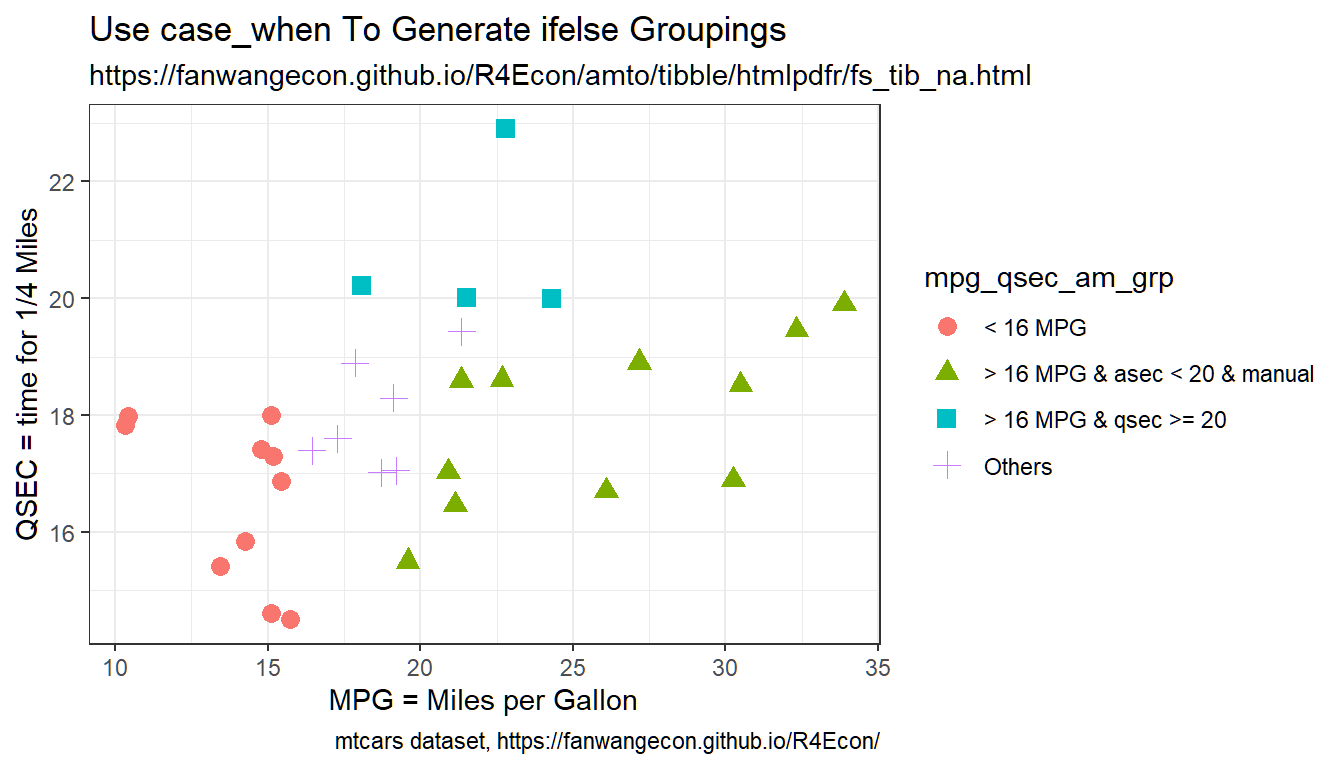
\includegraphics{Panel-Data-and-Optimization-with-R_files/figure-latex/unnamed-chunk-48-1} \end{center}

\hypertarget{drawly-random-rows}{%
\subsection{Drawly Random Rows}\label{drawly-random-rows}}

\begin{quote}
Go back to \href{http://fanwangecon.github.io/}{fan}'s \href{https://fanwangecon.github.io/REconTools/}{REconTools} Package, \href{https://fanwangecon.github.io/R4Econ/}{R Code Examples} Repository (\href{https://fanwangecon.github.io/R4Econ/bookdown}{bookdown site}), or \href{https://fanwangecon.github.io/Stat4Econ/}{Intro Stats with R} Repository (\href{https://fanwangecon.github.io/Stat4Econ/bookdown}{bookdown site}).
\end{quote}

\hypertarget{draw-random-subset-of-sample}{%
\subsubsection{Draw Random Subset of Sample}\label{draw-random-subset-of-sample}}

\begin{itemize}
\tightlist
\item
  r random discrete
\end{itemize}

We have a sample of N individuals in some dataframe. Draw without replacement a subset \(M<N\) of rows.

\begin{Shaded}
\begin{Highlighting}[]
\CommentTok{\# parameters, it\_M \textless{} it\_N}
\NormalTok{it\_N }\OtherTok{\textless{}{-}} \DecValTok{10}
\NormalTok{it\_M }\OtherTok{\textless{}{-}} \DecValTok{5}

\CommentTok{\# Draw it\_m from indexed list of it\_N}
\FunctionTok{set.seed}\NormalTok{(}\DecValTok{123}\NormalTok{)}
\NormalTok{ar\_it\_rand\_idx }\OtherTok{\textless{}{-}} \FunctionTok{sample}\NormalTok{(it\_N, it\_M, }\AttributeTok{replace=}\ConstantTok{FALSE}\NormalTok{)}

\CommentTok{\# dataframe}
\NormalTok{df\_full }\OtherTok{\textless{}{-}} \FunctionTok{as\_tibble}\NormalTok{(}\FunctionTok{matrix}\NormalTok{(}\FunctionTok{rnorm}\NormalTok{(}\DecValTok{4}\NormalTok{,}\AttributeTok{mean=}\DecValTok{0}\NormalTok{,}\AttributeTok{sd=}\DecValTok{1}\NormalTok{), }\AttributeTok{nrow=}\NormalTok{it\_N, }\AttributeTok{ncol=}\DecValTok{4}\NormalTok{)) }\SpecialCharTok{\%\textgreater{}\%} \FunctionTok{rowid\_to\_column}\NormalTok{(}\AttributeTok{var =} \StringTok{"ID"}\NormalTok{)}

\CommentTok{\# random Subset}
\NormalTok{df\_rand\_sub\_a }\OtherTok{\textless{}{-}}\NormalTok{ df\_full[ar\_it\_rand\_idx,]}

\CommentTok{\# Random subset also}
\NormalTok{df\_rand\_sub\_b }\OtherTok{\textless{}{-}}\NormalTok{ df\_full[}\FunctionTok{sample}\NormalTok{(}\FunctionTok{dim}\NormalTok{(df\_full)[}\DecValTok{1}\NormalTok{], it\_M, }\AttributeTok{replace=}\ConstantTok{FALSE}\NormalTok{),]}

\CommentTok{\# Print}
\CommentTok{\# Display}
\FunctionTok{kable}\NormalTok{(df\_full) }\SpecialCharTok{\%\textgreater{}\%} \FunctionTok{kable\_styling\_fc}\NormalTok{()}
\end{Highlighting}
\end{Shaded}

\begin{table}[!h]
\centering
\begin{tabular}{r|r|r|r|r}
\hline
ID & V1 & V2 & V3 & V4\\
\hline
\cellcolor{gray!6}{1} & \cellcolor{gray!6}{0.1292877} & \cellcolor{gray!6}{0.4609162} & \cellcolor{gray!6}{0.1292877} & \cellcolor{gray!6}{0.4609162}\\
\hline
2 & 1.7150650 & -1.2650612 & 1.7150650 & -1.2650612\\
\hline
\cellcolor{gray!6}{3} & \cellcolor{gray!6}{0.4609162} & \cellcolor{gray!6}{0.1292877} & \cellcolor{gray!6}{0.4609162} & \cellcolor{gray!6}{0.1292877}\\
\hline
4 & -1.2650612 & 1.7150650 & -1.2650612 & 1.7150650\\
\hline
\cellcolor{gray!6}{5} & \cellcolor{gray!6}{0.1292877} & \cellcolor{gray!6}{0.4609162} & \cellcolor{gray!6}{0.1292877} & \cellcolor{gray!6}{0.4609162}\\
\hline
6 & 1.7150650 & -1.2650612 & 1.7150650 & -1.2650612\\
\hline
\cellcolor{gray!6}{7} & \cellcolor{gray!6}{0.4609162} & \cellcolor{gray!6}{0.1292877} & \cellcolor{gray!6}{0.4609162} & \cellcolor{gray!6}{0.1292877}\\
\hline
8 & -1.2650612 & 1.7150650 & -1.2650612 & 1.7150650\\
\hline
\cellcolor{gray!6}{9} & \cellcolor{gray!6}{0.1292877} & \cellcolor{gray!6}{0.4609162} & \cellcolor{gray!6}{0.1292877} & \cellcolor{gray!6}{0.4609162}\\
\hline
10 & 1.7150650 & -1.2650612 & 1.7150650 & -1.2650612\\
\hline
\end{tabular}
\end{table}

\begin{Shaded}
\begin{Highlighting}[]
\FunctionTok{kable}\NormalTok{(df\_rand\_sub\_a) }\SpecialCharTok{\%\textgreater{}\%} \FunctionTok{kable\_styling\_fc}\NormalTok{()}
\end{Highlighting}
\end{Shaded}

\begin{table}[!h]
\centering
\begin{tabular}{r|r|r|r|r}
\hline
ID & V1 & V2 & V3 & V4\\
\hline
\cellcolor{gray!6}{3} & \cellcolor{gray!6}{0.4609162} & \cellcolor{gray!6}{0.1292877} & \cellcolor{gray!6}{0.4609162} & \cellcolor{gray!6}{0.1292877}\\
\hline
10 & 1.7150650 & -1.2650612 & 1.7150650 & -1.2650612\\
\hline
\cellcolor{gray!6}{2} & \cellcolor{gray!6}{1.7150650} & \cellcolor{gray!6}{-1.2650612} & \cellcolor{gray!6}{1.7150650} & \cellcolor{gray!6}{-1.2650612}\\
\hline
8 & -1.2650612 & 1.7150650 & -1.2650612 & 1.7150650\\
\hline
\cellcolor{gray!6}{6} & \cellcolor{gray!6}{1.7150650} & \cellcolor{gray!6}{-1.2650612} & \cellcolor{gray!6}{1.7150650} & \cellcolor{gray!6}{-1.2650612}\\
\hline
\end{tabular}
\end{table}

\begin{Shaded}
\begin{Highlighting}[]
\FunctionTok{kable}\NormalTok{(df\_rand\_sub\_b) }\SpecialCharTok{\%\textgreater{}\%} \FunctionTok{kable\_styling\_fc}\NormalTok{()}
\end{Highlighting}
\end{Shaded}

\begin{table}[!h]
\centering
\begin{tabular}{r|r|r|r|r}
\hline
ID & V1 & V2 & V3 & V4\\
\hline
\cellcolor{gray!6}{5} & \cellcolor{gray!6}{0.1292877} & \cellcolor{gray!6}{0.4609162} & \cellcolor{gray!6}{0.1292877} & \cellcolor{gray!6}{0.4609162}\\
\hline
3 & 0.4609162 & 0.1292877 & 0.4609162 & 0.1292877\\
\hline
\cellcolor{gray!6}{9} & \cellcolor{gray!6}{0.1292877} & \cellcolor{gray!6}{0.4609162} & \cellcolor{gray!6}{0.1292877} & \cellcolor{gray!6}{0.4609162}\\
\hline
1 & 0.1292877 & 0.4609162 & 0.1292877 & 0.4609162\\
\hline
\cellcolor{gray!6}{4} & \cellcolor{gray!6}{-1.2650612} & \cellcolor{gray!6}{1.7150650} & \cellcolor{gray!6}{-1.2650612} & \cellcolor{gray!6}{1.7150650}\\
\hline
\end{tabular}
\end{table}

\hypertarget{random-subset-of-panel}{%
\subsubsection{Random Subset of Panel}\label{random-subset-of-panel}}

There are \(N\) individuals, each could be observed \(M\) times, but then select a subset of rows only, so each person is randomly observed only a subset of times. Specifically, there there are 3 unique students with student ids, and the second variable shows the random dates in which the student showed up in class, out of the 10 classes available.

\begin{Shaded}
\begin{Highlighting}[]
\CommentTok{\# Define}
\NormalTok{it\_N }\OtherTok{\textless{}{-}} \DecValTok{3}
\NormalTok{it\_M }\OtherTok{\textless{}{-}} \DecValTok{10}
\NormalTok{svr\_id }\OtherTok{\textless{}{-}} \StringTok{\textquotesingle{}student\_id\textquotesingle{}}

\CommentTok{\# dataframe}
\FunctionTok{set.seed}\NormalTok{(}\DecValTok{123}\NormalTok{)}
\NormalTok{df\_panel\_rand }\OtherTok{\textless{}{-}} \FunctionTok{as\_tibble}\NormalTok{(}\FunctionTok{matrix}\NormalTok{(it\_M, }\AttributeTok{nrow=}\NormalTok{it\_N, }\AttributeTok{ncol=}\DecValTok{1}\NormalTok{)) }\SpecialCharTok{\%\textgreater{}\%}
  \FunctionTok{rowid\_to\_column}\NormalTok{(}\AttributeTok{var =}\NormalTok{ svr\_id) }\SpecialCharTok{\%\textgreater{}\%}
  \FunctionTok{uncount}\NormalTok{(V1) }\SpecialCharTok{\%\textgreater{}\%}
  \FunctionTok{group\_by}\NormalTok{(}\SpecialCharTok{!!}\FunctionTok{sym}\NormalTok{(svr\_id)) }\SpecialCharTok{\%\textgreater{}\%} \FunctionTok{mutate}\NormalTok{(}\AttributeTok{date =} \FunctionTok{row\_number}\NormalTok{()) }\SpecialCharTok{\%\textgreater{}\%}
  \FunctionTok{ungroup}\NormalTok{() }\SpecialCharTok{\%\textgreater{}\%} \FunctionTok{mutate}\NormalTok{(}\AttributeTok{in\_class =} \FunctionTok{case\_when}\NormalTok{(}\FunctionTok{rnorm}\NormalTok{(}\FunctionTok{n}\NormalTok{(),}\AttributeTok{mean=}\DecValTok{0}\NormalTok{,}\AttributeTok{sd=}\DecValTok{1}\NormalTok{) }\SpecialCharTok{\textless{}} \DecValTok{0} \SpecialCharTok{\textasciitilde{}} \DecValTok{1}\NormalTok{, }\ConstantTok{TRUE} \SpecialCharTok{\textasciitilde{}} \DecValTok{0}\NormalTok{)) }\SpecialCharTok{\%\textgreater{}\%}
  \FunctionTok{filter}\NormalTok{(in\_class }\SpecialCharTok{==} \DecValTok{1}\NormalTok{) }\SpecialCharTok{\%\textgreater{}\%} \FunctionTok{select}\NormalTok{(}\SpecialCharTok{!!}\FunctionTok{sym}\NormalTok{(svr\_id), date) }\SpecialCharTok{\%\textgreater{}\%}
  \FunctionTok{rename}\NormalTok{(}\AttributeTok{date\_in\_class =}\NormalTok{ date)}

\CommentTok{\# Print}
\FunctionTok{kable}\NormalTok{(df\_panel\_rand) }\SpecialCharTok{\%\textgreater{}\%} \FunctionTok{kable\_styling\_fc}\NormalTok{()}
\end{Highlighting}
\end{Shaded}

\begin{table}[!h]
\centering
\begin{tabular}{r|r}
\hline
student\_id & date\_in\_class\\
\hline
\cellcolor{gray!6}{1} & \cellcolor{gray!6}{1}\\
\hline
1 & 2\\
\hline
\cellcolor{gray!6}{1} & \cellcolor{gray!6}{8}\\
\hline
1 & 9\\
\hline
\cellcolor{gray!6}{1} & \cellcolor{gray!6}{10}\\
\hline
2 & 5\\
\hline
\cellcolor{gray!6}{2} & \cellcolor{gray!6}{8}\\
\hline
2 & 10\\
\hline
\cellcolor{gray!6}{3} & \cellcolor{gray!6}{1}\\
\hline
3 & 2\\
\hline
\cellcolor{gray!6}{3} & \cellcolor{gray!6}{3}\\
\hline
3 & 4\\
\hline
\cellcolor{gray!6}{3} & \cellcolor{gray!6}{5}\\
\hline
3 & 6\\
\hline
\cellcolor{gray!6}{3} & \cellcolor{gray!6}{9}\\
\hline
\end{tabular}
\end{table}

\hypertarget{generate-variables-conditional-on-others}{%
\subsection{Generate Variables Conditional On Others}\label{generate-variables-conditional-on-others}}

\begin{quote}
Go back to \href{http://fanwangecon.github.io/}{fan}'s \href{https://fanwangecon.github.io/REconTools/}{REconTools} Package, \href{https://fanwangecon.github.io/R4Econ/}{R Code Examples} Repository (\href{https://fanwangecon.github.io/R4Econ/bookdown}{bookdown site}), or \href{https://fanwangecon.github.io/Stat4Econ/}{Intro Stats with R} Repository (\href{https://fanwangecon.github.io/Stat4Econ/bookdown}{bookdown site}).
\end{quote}

\hypertarget{case_when-basic-example}{%
\subsubsection{case\_when Basic Example}\label{case_when-basic-example}}

Given several other variables, and generate a new variable when these varaibles satisfy conditions. Note that case\_when are ifelse type statements. So below

\begin{enumerate}
\def\labelenumi{\arabic{enumi}.}
\tightlist
\item
  group one is below 16 MPG
\item
  when do \emph{qsec \textgreater= 20} second line that is elseif, only those that are \emph{\textgreater=16} are considered here
\item
  then think about two dimensional mpg and qsec grid, the lower-right area, give another category to manual cars in that group
\end{enumerate}

\begin{Shaded}
\begin{Highlighting}[]
\CommentTok{\# Get mtcars}
\NormalTok{df\_mtcars }\OtherTok{\textless{}{-}}\NormalTok{ mtcars}

\CommentTok{\# case\_when with mtcars}
\NormalTok{df\_mtcars }\OtherTok{\textless{}{-}}\NormalTok{ df\_mtcars }\SpecialCharTok{\%\textgreater{}\%}
  \FunctionTok{mutate}\NormalTok{(}\AttributeTok{mpg\_qsec\_am\_grp =} 
           \FunctionTok{case\_when}\NormalTok{(mpg }\SpecialCharTok{\textless{}} \DecValTok{16} \SpecialCharTok{\textasciitilde{}} \StringTok{"\textless{} 16 MPG"}\NormalTok{,}
\NormalTok{                     qsec }\SpecialCharTok{\textgreater{}=} \DecValTok{20} \SpecialCharTok{\textasciitilde{}} \StringTok{"\textgreater{} 16 MPG \& qsec \textgreater{}= 20"}\NormalTok{,}
\NormalTok{                     am }\SpecialCharTok{==} \DecValTok{1} \SpecialCharTok{\textasciitilde{}} \StringTok{"\textgreater{} 16 MPG \& asec \textless{} 20 \& manual"}\NormalTok{,}
                     \ConstantTok{TRUE} \SpecialCharTok{\textasciitilde{}} \StringTok{"Others"}\NormalTok{))}

\CommentTok{\# \# For dataframe}
\CommentTok{\# df.reg \textless{}{-}df.reg \%\textgreater{}\% na\_if({-}Inf) \%\textgreater{}\% na\_if(Inf)}
\CommentTok{\# \# For a specific variable in dataframe}
\CommentTok{\# df.reg.use \%\textgreater{}\% mutate(!!(var.input) := na\_if(!!sym(var.input), 0))}
\CommentTok{\# }
\CommentTok{\# \# Setting to NA}
\CommentTok{\# df.reg.use \textless{}{-} df.reg.guat \%\textgreater{}\% filter(!!sym(var.mth) != 0)}
\CommentTok{\# df.reg.use.log \textless{}{-} df.reg.use}
\CommentTok{\# df.reg.use.log[which(is.nan(df.reg.use$prot.imputed.log)),] = NA}
\CommentTok{\# df.reg.use.log[which(df.reg.use$prot.imputed.log==Inf),] = NA}
\CommentTok{\# df.reg.use.log[which(df.reg.use$prot.imputed.log=={-}Inf),] = NA}
\CommentTok{\# df.reg.use.log \textless{}{-} df.reg.use.log \%\textgreater{}\% drop\_na(prot.imputed.log)}
\CommentTok{\# \# df.reg.use.log$prot.imputed.log}
\end{Highlighting}
\end{Shaded}

Now we generate scatter plot based on the combined factors

\begin{Shaded}
\begin{Highlighting}[]
\CommentTok{\# Labeling}
\NormalTok{st\_title }\OtherTok{\textless{}{-}} \FunctionTok{paste0}\NormalTok{(}\StringTok{\textquotesingle{}Use case\_when To Generate ifelse Groupings\textquotesingle{}}\NormalTok{)}
\NormalTok{st\_subtitle }\OtherTok{\textless{}{-}} \FunctionTok{paste0}\NormalTok{(}\StringTok{\textquotesingle{}https://fanwangecon.github.io/\textquotesingle{}}\NormalTok{,}
                      \StringTok{\textquotesingle{}R4Econ/amto/tibble/htmlpdfr/fs\_tib\_na.html\textquotesingle{}}\NormalTok{)}
\NormalTok{st\_caption }\OtherTok{\textless{}{-}} \FunctionTok{paste0}\NormalTok{(}\StringTok{\textquotesingle{}mtcars dataset, \textquotesingle{}}\NormalTok{,}
                     \StringTok{\textquotesingle{}https://fanwangecon.github.io/R4Econ/\textquotesingle{}}\NormalTok{)}
\NormalTok{st\_x\_label }\OtherTok{\textless{}{-}} \StringTok{\textquotesingle{}MPG = Miles per Gallon\textquotesingle{}}
\NormalTok{st\_y\_label }\OtherTok{\textless{}{-}} \StringTok{\textquotesingle{}QSEC = time for 1/4 Miles\textquotesingle{}}

\CommentTok{\# Graphing}
\NormalTok{plt\_mtcars\_casewhen\_scatter }\OtherTok{\textless{}{-}} 
  \FunctionTok{ggplot}\NormalTok{(df\_mtcars, }
         \FunctionTok{aes}\NormalTok{(}\AttributeTok{x=}\NormalTok{mpg, }\AttributeTok{y=}\NormalTok{qsec, }
             \AttributeTok{colour=}\NormalTok{mpg\_qsec\_am\_grp, }
             \AttributeTok{shape=}\NormalTok{mpg\_qsec\_am\_grp)) }\SpecialCharTok{+}
  \FunctionTok{geom\_jitter}\NormalTok{(}\AttributeTok{size=}\DecValTok{3}\NormalTok{, }\AttributeTok{width =} \FloatTok{0.15}\NormalTok{) }\SpecialCharTok{+}
  \FunctionTok{labs}\NormalTok{(}\AttributeTok{title =}\NormalTok{ st\_title, }\AttributeTok{subtitle =}\NormalTok{ st\_subtitle,}
       \AttributeTok{x =}\NormalTok{ st\_x\_label, }\AttributeTok{y =}\NormalTok{ st\_y\_label, }\AttributeTok{caption =}\NormalTok{ st\_caption) }\SpecialCharTok{+}
  \FunctionTok{theme\_bw}\NormalTok{()}

\CommentTok{\# show}
\FunctionTok{print}\NormalTok{(plt\_mtcars\_casewhen\_scatter)}
\end{Highlighting}
\end{Shaded}

\begin{center}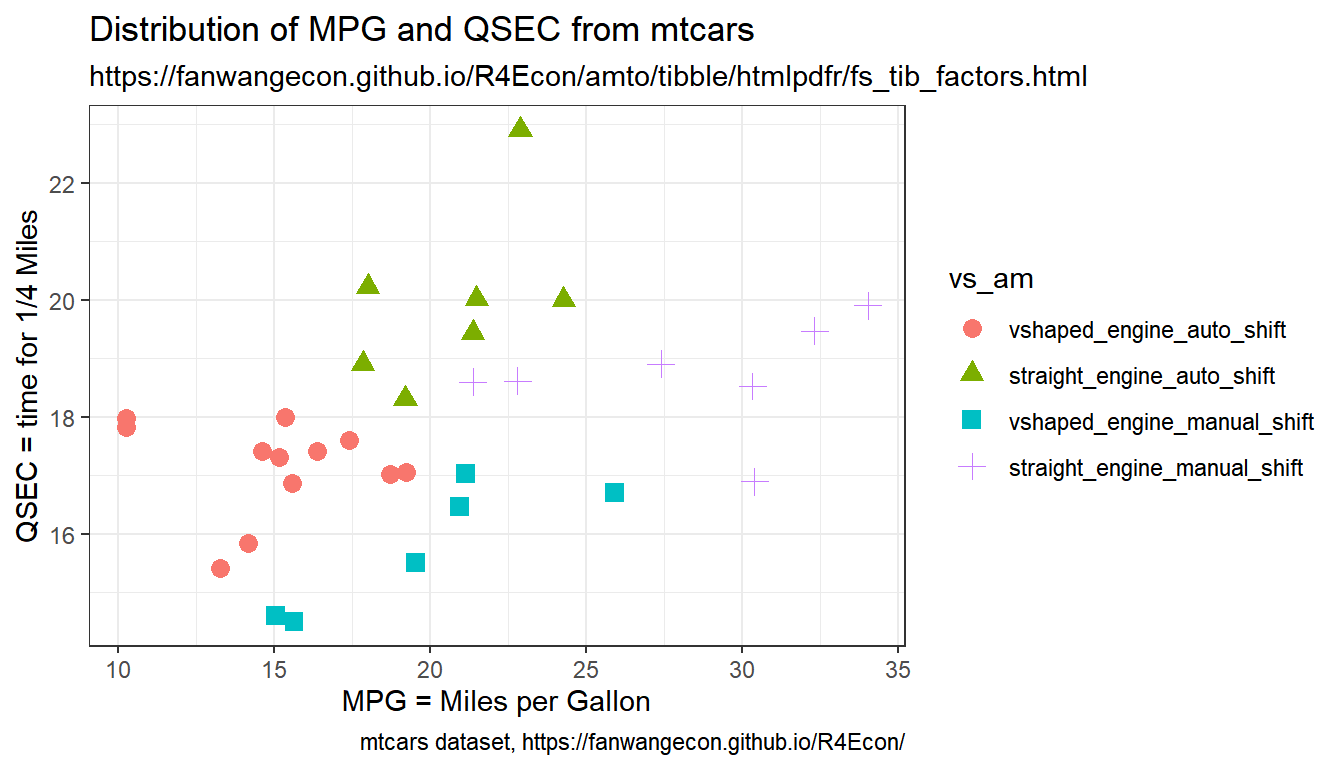
\includegraphics{Panel-Data-and-Optimization-with-R_files/figure-latex/unnamed-chunk-53-1} \end{center}

\hypertarget{generate-na-values-if-variables-have-certain-value}{%
\subsubsection{Generate NA values if Variables have Certain Value}\label{generate-na-values-if-variables-have-certain-value}}

In the example below, in one line:

\begin{enumerate}
\def\labelenumi{\arabic{enumi}.}
\tightlist
\item
  generate a random standard normal vector
\item
  two set na methods:

  \begin{itemize}
  \tightlist
  \item
    if the value of the standard normal is negative, set value to -999, otherwise MPG, replace the value \emph{-999} with \emph{NA}
  \item
    case\_when only with type specific NA values
  \item
    \href{https://github.com/tidyverse/dplyr/issues/3202\#issuecomment-343601409}{Assigning NA yields error in case\_when}
  \item
    note we need to conform NA to type
  \end{itemize}
\item
  generate new categorical variable based on NA condition using is.na with both string and numeric NAs jointly considered.

  \begin{itemize}
  \tightlist
  \item
    fake NA string to be printed on chart
  \end{itemize}
\end{enumerate}

\begin{Shaded}
\begin{Highlighting}[]
\CommentTok{\# Get mtcars}
\NormalTok{df\_mtcars }\OtherTok{\textless{}{-}}\NormalTok{ mtcars}

\CommentTok{\# Make some values of mpg randomly NA}
\CommentTok{\# the NA has to conform to the type of the remaining values for the new variable}
\CommentTok{\# NA\_real\_, NA\_character\_, NA\_integer\_, NA\_complex\_}
\FunctionTok{set.seed}\NormalTok{(}\DecValTok{2341}\NormalTok{)}
\NormalTok{df\_mtcars }\OtherTok{\textless{}{-}}\NormalTok{ df\_mtcars }\SpecialCharTok{\%\textgreater{}\%} 
  \FunctionTok{mutate}\NormalTok{(}\AttributeTok{mpg\_wth\_NA1 =} \FunctionTok{na\_if}\NormalTok{(}
    \FunctionTok{case\_when}\NormalTok{(}
      \FunctionTok{rnorm}\NormalTok{(}\FunctionTok{n}\NormalTok{(),}\AttributeTok{mean=}\DecValTok{0}\NormalTok{,}\AttributeTok{sd=}\DecValTok{1}\NormalTok{) }\SpecialCharTok{\textless{}} \DecValTok{0} \SpecialCharTok{\textasciitilde{}} \SpecialCharTok{{-}}\DecValTok{999}\NormalTok{, }
      \ConstantTok{TRUE} \SpecialCharTok{\textasciitilde{}}\NormalTok{ mpg), }
    \SpecialCharTok{{-}}\DecValTok{999}\NormalTok{)) }\SpecialCharTok{\%\textgreater{}\%}
  \FunctionTok{mutate}\NormalTok{(}\AttributeTok{mpg\_wth\_NA2 =} \FunctionTok{case\_when}\NormalTok{(}
    \FunctionTok{rnorm}\NormalTok{(}\FunctionTok{n}\NormalTok{(),}\AttributeTok{mean=}\DecValTok{0}\NormalTok{,}\AttributeTok{sd=}\DecValTok{1}\NormalTok{) }\SpecialCharTok{\textless{}} \DecValTok{0} \SpecialCharTok{\textasciitilde{}} \ConstantTok{NA\_real\_}\NormalTok{, }
    \ConstantTok{TRUE} \SpecialCharTok{\textasciitilde{}}\NormalTok{ mpg)) }\SpecialCharTok{\%\textgreater{}\%}
  \FunctionTok{mutate}\NormalTok{(}\AttributeTok{mpg\_wth\_NA3 =} \FunctionTok{case\_when}\NormalTok{(}
    \FunctionTok{rnorm}\NormalTok{(}\FunctionTok{n}\NormalTok{(),}\AttributeTok{mean=}\DecValTok{0}\NormalTok{,}\AttributeTok{sd=}\DecValTok{1}\NormalTok{) }\SpecialCharTok{\textless{}} \DecValTok{0} \SpecialCharTok{\textasciitilde{}} \ConstantTok{NA\_character\_}\NormalTok{, }
    \ConstantTok{TRUE} \SpecialCharTok{\textasciitilde{}} \StringTok{"shock \textgreater{} 0 string"}\NormalTok{))}
  
\CommentTok{\# Generate New Variables based on if mpg\_wth\_NA is NA or not}
\CommentTok{\# same variable as above, but now first a category based on if NA}
\CommentTok{\# And we generate a fake string "NA" variable, this is not NA}
\CommentTok{\# the String NA allows for it to be printed on figure}
\NormalTok{df\_mtcars }\OtherTok{\textless{}{-}}\NormalTok{ df\_mtcars }\SpecialCharTok{\%\textgreater{}\%}
  \FunctionTok{mutate}\NormalTok{(}\AttributeTok{group\_with\_na =} 
           \FunctionTok{case\_when}\NormalTok{(}\FunctionTok{is.na}\NormalTok{(mpg\_wth\_NA2) }\SpecialCharTok{\&} \FunctionTok{is.na}\NormalTok{(mpg\_wth\_NA3) }\SpecialCharTok{\textasciitilde{}} 
                       \StringTok{"Rand String and Rand Numeric both NA"}\NormalTok{, }
\NormalTok{                     mpg }\SpecialCharTok{\textless{}} \DecValTok{16} \SpecialCharTok{\textasciitilde{}} \StringTok{"\textless{} 16 MPG"}\NormalTok{,}
\NormalTok{                     qsec }\SpecialCharTok{\textgreater{}=} \DecValTok{20} \SpecialCharTok{\textasciitilde{}} \StringTok{"\textgreater{} 16 MPG \& qsec \textgreater{}= 20"}\NormalTok{,}
\NormalTok{                     am }\SpecialCharTok{==} \DecValTok{1} \SpecialCharTok{\textasciitilde{}} \StringTok{"\textgreater{} 16 MPG \& asec \textless{} 20 \& manual"}\NormalTok{,}
                     \ConstantTok{TRUE} \SpecialCharTok{\textasciitilde{}} \StringTok{"Fake String NA"}\NormalTok{))}

\CommentTok{\# show}
\FunctionTok{kable}\NormalTok{(}\FunctionTok{head}\NormalTok{(df\_mtcars }\SpecialCharTok{\%\textgreater{}\%} \FunctionTok{select}\NormalTok{(}\FunctionTok{starts\_with}\NormalTok{(}\StringTok{\textquotesingle{}mpg\textquotesingle{}}\NormalTok{)),}\DecValTok{13}\NormalTok{)) }\SpecialCharTok{\%\textgreater{}\%}
  \FunctionTok{kable\_styling\_fc}\NormalTok{()}
\end{Highlighting}
\end{Shaded}

\begin{table}[!h]
\centering
\begin{tabular}{r|r|r|l}
\hline
mpg & mpg\_wth\_NA1 & mpg\_wth\_NA2 & mpg\_wth\_NA3\\
\hline
\cellcolor{gray!6}{21.0} & \cellcolor{gray!6}{NA} & \cellcolor{gray!6}{NA} & \cellcolor{gray!6}{shock > 0 string}\\
\hline
21.0 & 21.0 & 21.0 & NA\\
\hline
\cellcolor{gray!6}{22.8} & \cellcolor{gray!6}{NA} & \cellcolor{gray!6}{NA} & \cellcolor{gray!6}{NA}\\
\hline
21.4 & NA & 21.4 & NA\\
\hline
\cellcolor{gray!6}{18.7} & \cellcolor{gray!6}{NA} & \cellcolor{gray!6}{18.7} & \cellcolor{gray!6}{NA}\\
\hline
18.1 & 18.1 & NA & shock > 0 string\\
\hline
\cellcolor{gray!6}{14.3} & \cellcolor{gray!6}{14.3} & \cellcolor{gray!6}{NA} & \cellcolor{gray!6}{shock > 0 string}\\
\hline
24.4 & NA & 24.4 & NA\\
\hline
\cellcolor{gray!6}{22.8} & \cellcolor{gray!6}{22.8} & \cellcolor{gray!6}{22.8} & \cellcolor{gray!6}{NA}\\
\hline
19.2 & 19.2 & NA & NA\\
\hline
\cellcolor{gray!6}{17.8} & \cellcolor{gray!6}{NA} & \cellcolor{gray!6}{NA} & \cellcolor{gray!6}{NA}\\
\hline
16.4 & 16.4 & 16.4 & NA\\
\hline
\cellcolor{gray!6}{17.3} & \cellcolor{gray!6}{NA} & \cellcolor{gray!6}{NA} & \cellcolor{gray!6}{shock > 0 string}\\
\hline
\end{tabular}
\end{table}

\begin{Shaded}
\begin{Highlighting}[]
\CommentTok{\# \# Setting to NA}
\CommentTok{\# df.reg.use \textless{}{-} df.reg.guat \%\textgreater{}\% filter(!!sym(var.mth) != 0)}
\CommentTok{\# df.reg.use.log \textless{}{-} df.reg.use}
\CommentTok{\# df.reg.use.log[which(is.nan(df.reg.use$prot.imputed.log)),] = NA}
\CommentTok{\# df.reg.use.log[which(df.reg.use$prot.imputed.log==Inf),] = NA}
\CommentTok{\# df.reg.use.log[which(df.reg.use$prot.imputed.log=={-}Inf),] = NA}
\CommentTok{\# df.reg.use.log \textless{}{-} df.reg.use.log \%\textgreater{}\% drop\_na(prot.imputed.log)}
\CommentTok{\# \# df.reg.use.log$prot.imputed.log}
\end{Highlighting}
\end{Shaded}

Now we generate scatter plot based on the combined factors, but now with the NA category

\begin{Shaded}
\begin{Highlighting}[]
\CommentTok{\# Labeling}
\NormalTok{st\_title }\OtherTok{\textless{}{-}} \FunctionTok{paste0}\NormalTok{(}\StringTok{\textquotesingle{}Use na\_if and is.na to Generate and Distinguish NA Values}\SpecialCharTok{\textbackslash{}n}\StringTok{\textquotesingle{}}\NormalTok{,}
                   \StringTok{\textquotesingle{}NA\_real\_, NA\_character\_, NA\_integer\_, NA\_complex\_\textquotesingle{}}\NormalTok{)}
\NormalTok{st\_subtitle }\OtherTok{\textless{}{-}} \FunctionTok{paste0}\NormalTok{(}\StringTok{\textquotesingle{}https://fanwangecon.github.io/\textquotesingle{}}\NormalTok{,}
                      \StringTok{\textquotesingle{}R4Econ/amto/tibble/htmlpdfr/fs\_tib\_na.html\textquotesingle{}}\NormalTok{)}
\NormalTok{st\_caption }\OtherTok{\textless{}{-}} \FunctionTok{paste0}\NormalTok{(}\StringTok{\textquotesingle{}mtcars dataset, \textquotesingle{}}\NormalTok{,}
                     \StringTok{\textquotesingle{}https://fanwangecon.github.io/R4Econ/\textquotesingle{}}\NormalTok{)}
\NormalTok{st\_x\_label }\OtherTok{\textless{}{-}} \StringTok{\textquotesingle{}MPG = Miles per Gallon\textquotesingle{}}
\NormalTok{st\_y\_label }\OtherTok{\textless{}{-}} \StringTok{\textquotesingle{}QSEC = time for 1/4 Miles\textquotesingle{}}

\CommentTok{\# Graphing}
\NormalTok{plt\_mtcars\_ifisna\_scatter }\OtherTok{\textless{}{-}} 
  \FunctionTok{ggplot}\NormalTok{(df\_mtcars, }
         \FunctionTok{aes}\NormalTok{(}\AttributeTok{x=}\NormalTok{mpg, }\AttributeTok{y=}\NormalTok{qsec, }
             \AttributeTok{colour=}\NormalTok{group\_with\_na, }
             \AttributeTok{shape=}\NormalTok{group\_with\_na)) }\SpecialCharTok{+}
  \FunctionTok{geom\_jitter}\NormalTok{(}\AttributeTok{size=}\DecValTok{3}\NormalTok{, }\AttributeTok{width =} \FloatTok{0.15}\NormalTok{) }\SpecialCharTok{+}
  \FunctionTok{labs}\NormalTok{(}\AttributeTok{title =}\NormalTok{ st\_title, }\AttributeTok{subtitle =}\NormalTok{ st\_subtitle,}
       \AttributeTok{x =}\NormalTok{ st\_x\_label, }\AttributeTok{y =}\NormalTok{ st\_y\_label, }\AttributeTok{caption =}\NormalTok{ st\_caption) }\SpecialCharTok{+}
  \FunctionTok{theme\_bw}\NormalTok{()}

\CommentTok{\# show}
\FunctionTok{print}\NormalTok{(plt\_mtcars\_ifisna\_scatter)}
\end{Highlighting}
\end{Shaded}

\begin{center}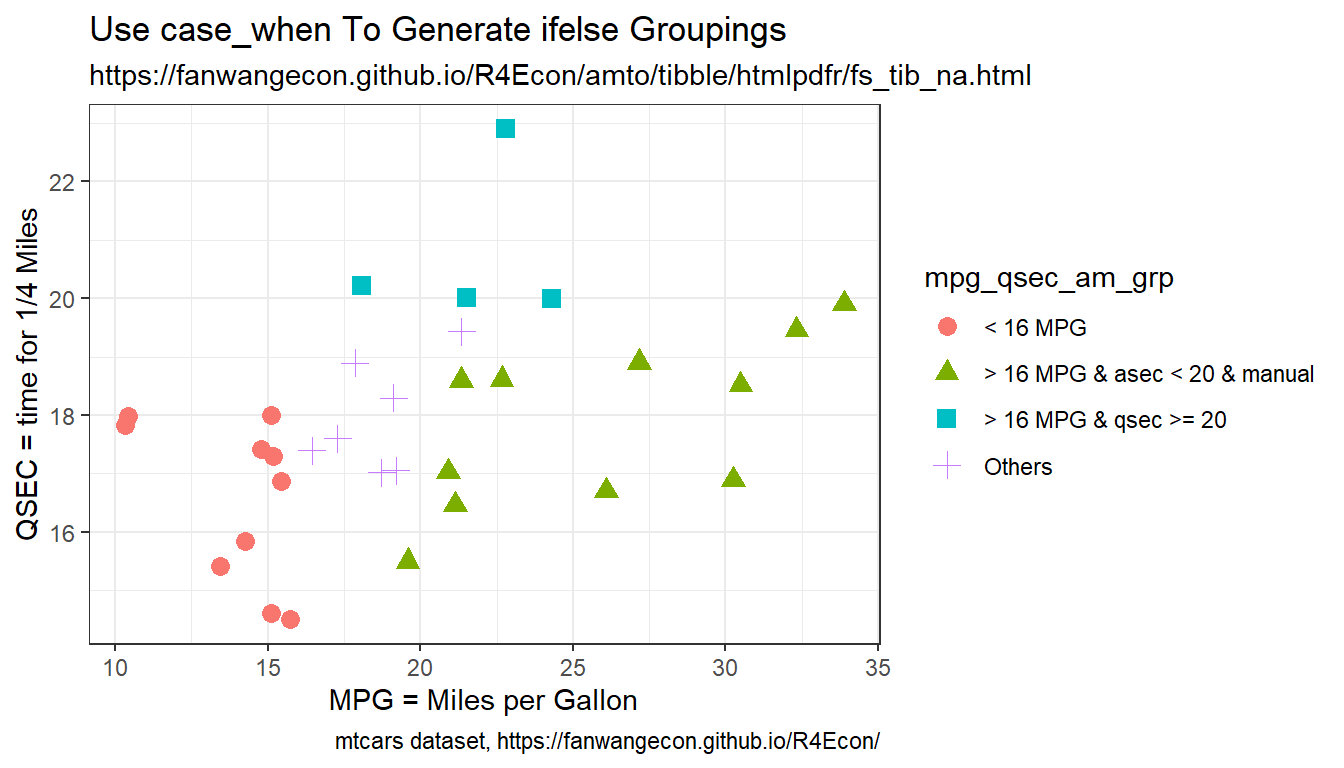
\includegraphics{Panel-Data-and-Optimization-with-R_files/figure-latex/unnamed-chunk-55-1} \end{center}

\hypertarget{approximate-values-comparison}{%
\subsubsection{Approximate Values Comparison}\label{approximate-values-comparison}}

\begin{itemize}
\tightlist
\item
  r values almost the same
\item
  \href{https://stat.ethz.ch/R-manual/R-patched/library/base/html/all.equal.html}{all.equal}
\end{itemize}

From numeric approximation, often values are very close, and should be set to equal. Use \emph{isTRUE(all.equal)}. In the example below, we randomly generates four arrays. Two of the arrays have slightly higher variance, two arrays have slightly lower variance. They sd are to be 10 times below or 10 times above the tolerance comparison level. The values are not the same in any of the columns, but by allowing for almost true given some tolerance level, in the low standard deviation case, the values differences are within tolerance, so they are equal.

This is an essential issue when dealing with optimization results.

\begin{Shaded}
\begin{Highlighting}[]
\CommentTok{\# Set tolerance }
\NormalTok{tol\_lvl }\OtherTok{=} \FloatTok{1.5e{-}3}
\NormalTok{sd\_lower\_than\_tol }\OtherTok{=}\NormalTok{ tol\_lvl}\SpecialCharTok{/}\DecValTok{10}
\NormalTok{sd\_higher\_than\_tol }\OtherTok{=}\NormalTok{ tol\_lvl}\SpecialCharTok{*}\DecValTok{10}

\CommentTok{\# larger SD}
\FunctionTok{set.seed}\NormalTok{(}\DecValTok{123}\NormalTok{)}
\NormalTok{mt\_runif\_standard }\OtherTok{\textless{}{-}} \FunctionTok{matrix}\NormalTok{(}\FunctionTok{rnorm}\NormalTok{(}\DecValTok{10}\NormalTok{,}\AttributeTok{mean=}\DecValTok{0}\NormalTok{,}\AttributeTok{sd=}\NormalTok{sd\_higher\_than\_tol), }\AttributeTok{nrow=}\DecValTok{5}\NormalTok{, }\AttributeTok{ncol=}\DecValTok{2}\NormalTok{)}

\CommentTok{\# small SD}
\FunctionTok{set.seed}\NormalTok{(}\DecValTok{123}\NormalTok{)}
\NormalTok{mt\_rnorm\_small\_sd }\OtherTok{\textless{}{-}} \FunctionTok{matrix}\NormalTok{(}\FunctionTok{rnorm}\NormalTok{(}\DecValTok{10}\NormalTok{,}\AttributeTok{mean=}\DecValTok{0}\NormalTok{,}\AttributeTok{sd=}\NormalTok{sd\_lower\_than\_tol), }\AttributeTok{nrow=}\DecValTok{5}\NormalTok{, }\AttributeTok{ncol=}\DecValTok{2}\NormalTok{)}

\CommentTok{\# Generates Random Matirx}
\NormalTok{tb\_rnorm\_runif }\OtherTok{\textless{}{-}} \FunctionTok{as\_tibble}\NormalTok{(}\FunctionTok{cbind}\NormalTok{(mt\_rnorm\_small\_sd, mt\_runif\_standard))}

\CommentTok{\# Are Variables the same, not for strict comparison}
\NormalTok{tb\_rnorm\_runif\_approxi\_same }\OtherTok{\textless{}{-}}\NormalTok{ tb\_rnorm\_runif }\SpecialCharTok{\%\textgreater{}\%}
  \FunctionTok{mutate}\NormalTok{(}\AttributeTok{V1\_V2\_ALMOST\_SAME =} 
           \FunctionTok{case\_when}\NormalTok{(}\FunctionTok{isTRUE}\NormalTok{(}\FunctionTok{all.equal}\NormalTok{(V1, V2, }\AttributeTok{tolerance=}\NormalTok{tol\_lvl)) }\SpecialCharTok{\textasciitilde{}} 
                       \FunctionTok{paste0}\NormalTok{(}\StringTok{\textquotesingle{}TOL=\textquotesingle{}}\NormalTok{,sd\_lower\_than\_tol,}\StringTok{\textquotesingle{}, SAME ALMOST\textquotesingle{}}\NormalTok{),}
                     \ConstantTok{TRUE} \SpecialCharTok{\textasciitilde{}} 
                       \FunctionTok{paste0}\NormalTok{(}\StringTok{\textquotesingle{}TOL=\textquotesingle{}}\NormalTok{,sd\_lower\_than\_tol,}\StringTok{\textquotesingle{}, NOT SAME ALMOST\textquotesingle{}}\NormalTok{))) }\SpecialCharTok{\%\textgreater{}\%}
  \FunctionTok{mutate}\NormalTok{(}\AttributeTok{V3\_V4\_ALMOST\_SAME =}
           \FunctionTok{case\_when}\NormalTok{(}\FunctionTok{isTRUE}\NormalTok{(}\FunctionTok{all.equal}\NormalTok{(V3, V4, }\AttributeTok{tolerance=}\NormalTok{tol\_lvl)) }\SpecialCharTok{\textasciitilde{}} 
                       \FunctionTok{paste0}\NormalTok{(}\StringTok{\textquotesingle{}TOL=\textquotesingle{}}\NormalTok{,sd\_higher\_than\_tol,}\StringTok{\textquotesingle{}, SAME ALMOST\textquotesingle{}}\NormalTok{),}
                     \ConstantTok{TRUE} \SpecialCharTok{\textasciitilde{}} 
                       \FunctionTok{paste0}\NormalTok{(}\StringTok{\textquotesingle{}TOL=\textquotesingle{}}\NormalTok{,sd\_higher\_than\_tol,}\StringTok{\textquotesingle{}, NOT SAME ALMOST\textquotesingle{}}\NormalTok{)))}

\CommentTok{\# Pring}
\FunctionTok{kable}\NormalTok{(tb\_rnorm\_runif\_approxi\_same) }\SpecialCharTok{\%\textgreater{}\%} \FunctionTok{kable\_styling\_fc\_wide}\NormalTok{()}
\end{Highlighting}
\end{Shaded}

\begin{table}[!h]
\centering
\resizebox{\linewidth}{!}{
\begin{tabular}{r|r|r|r|l|l}
\hline
V1 & V2 & V3 & V4 & V1\_V2\_ALMOST\_SAME & V3\_V4\_ALMOST\_SAME\\
\hline
\cellcolor{gray!6}{-0.0000841} & \cellcolor{gray!6}{0.0002573} & \cellcolor{gray!6}{-0.0084071} & \cellcolor{gray!6}{0.0257260} & \cellcolor{gray!6}{TOL=0.00015, SAME ALMOST} & \cellcolor{gray!6}{TOL=0.015, NOT SAME ALMOST}\\
\hline
-0.0000345 & 0.0000691 & -0.0034527 & 0.0069137 & TOL=0.00015, SAME ALMOST & TOL=0.015, NOT SAME ALMOST\\
\hline
\cellcolor{gray!6}{0.0002338} & \cellcolor{gray!6}{-0.0001898} & \cellcolor{gray!6}{0.0233806} & \cellcolor{gray!6}{-0.0189759} & \cellcolor{gray!6}{TOL=0.00015, SAME ALMOST} & \cellcolor{gray!6}{TOL=0.015, NOT SAME ALMOST}\\
\hline
0.0000106 & -0.0001030 & 0.0010576 & -0.0103028 & TOL=0.00015, SAME ALMOST & TOL=0.015, NOT SAME ALMOST\\
\hline
\cellcolor{gray!6}{0.0000194} & \cellcolor{gray!6}{-0.0000668} & \cellcolor{gray!6}{0.0019393} & \cellcolor{gray!6}{-0.0066849} & \cellcolor{gray!6}{TOL=0.00015, SAME ALMOST} & \cellcolor{gray!6}{TOL=0.015, NOT SAME ALMOST}\\
\hline
\end{tabular}}
\end{table}

\hypertarget{string-dataframes}{%
\subsection{String Dataframes}\label{string-dataframes}}

\begin{quote}
Go back to \href{http://fanwangecon.github.io/}{fan}'s \href{https://fanwangecon.github.io/REconTools/}{REconTools} Package, \href{https://fanwangecon.github.io/R4Econ/}{R Code Examples} Repository (\href{https://fanwangecon.github.io/R4Econ/bookdown}{bookdown site}), or \href{https://fanwangecon.github.io/Stat4Econ/}{Intro Stats with R} Repository (\href{https://fanwangecon.github.io/Stat4Econ/bookdown}{bookdown site}).
\end{quote}

\hypertarget{list-of-strings-to-tibble-datfare}{%
\subsubsection{List of Strings to Tibble Datfare}\label{list-of-strings-to-tibble-datfare}}

There are several lists of strings, store them as variables in a dataframe.

\begin{Shaded}
\begin{Highlighting}[]
\CommentTok{\# Sting data inputs}
\NormalTok{ls\_st\_abc }\OtherTok{\textless{}{-}} \FunctionTok{c}\NormalTok{(}\StringTok{\textquotesingle{}a\textquotesingle{}}\NormalTok{, }\StringTok{\textquotesingle{}b\textquotesingle{}}\NormalTok{, }\StringTok{\textquotesingle{}c\textquotesingle{}}\NormalTok{)}
\NormalTok{ls\_st\_efg }\OtherTok{\textless{}{-}} \FunctionTok{c}\NormalTok{(}\StringTok{\textquotesingle{}e\textquotesingle{}}\NormalTok{, }\StringTok{\textquotesingle{}f\textquotesingle{}}\NormalTok{, }\StringTok{\textquotesingle{}g\textquotesingle{}}\NormalTok{)}
\NormalTok{ls\_st\_opq }\OtherTok{\textless{}{-}} \FunctionTok{c}\NormalTok{(}\StringTok{\textquotesingle{}o\textquotesingle{}}\NormalTok{, }\StringTok{\textquotesingle{}p\textquotesingle{}}\NormalTok{, }\StringTok{\textquotesingle{}q\textquotesingle{}}\NormalTok{)}
\NormalTok{mt\_str }\OtherTok{=} \FunctionTok{cbind}\NormalTok{(ls\_st\_abc, ls\_st\_efg, ls\_st\_opq)}

\CommentTok{\# Column Names}
\NormalTok{ar\_st\_varnames }\OtherTok{\textless{}{-}} \FunctionTok{c}\NormalTok{(}\StringTok{\textquotesingle{}id\textquotesingle{}}\NormalTok{,}\StringTok{\textquotesingle{}var1\textquotesingle{}}\NormalTok{,}\StringTok{\textquotesingle{}var2\textquotesingle{}}\NormalTok{,}\StringTok{\textquotesingle{}var3\textquotesingle{}}\NormalTok{)}

\CommentTok{\# Combine to tibble, add name col1, col2, etc.}
\NormalTok{tb\_st\_combine }\OtherTok{\textless{}{-}} \FunctionTok{as\_tibble}\NormalTok{(mt\_str) }\SpecialCharTok{\%\textgreater{}\%}
  \FunctionTok{rowid\_to\_column}\NormalTok{(}\AttributeTok{var =} \StringTok{"id"}\NormalTok{) }\SpecialCharTok{\%\textgreater{}\%}
  \FunctionTok{rename\_all}\NormalTok{(}\SpecialCharTok{\textasciitilde{}}\FunctionTok{c}\NormalTok{(ar\_st\_varnames))}

\CommentTok{\# Display}
\FunctionTok{kable}\NormalTok{(tb\_st\_combine) }\SpecialCharTok{\%\textgreater{}\%} \FunctionTok{kable\_styling\_fc}\NormalTok{()}
\end{Highlighting}
\end{Shaded}

\begin{table}[!h]
\centering
\begin{tabular}{r|l|l|l}
\hline
id & var1 & var2 & var3\\
\hline
\cellcolor{gray!6}{1} & \cellcolor{gray!6}{a} & \cellcolor{gray!6}{e} & \cellcolor{gray!6}{o}\\
\hline
2 & b & f & p\\
\hline
\cellcolor{gray!6}{3} & \cellcolor{gray!6}{c} & \cellcolor{gray!6}{g} & \cellcolor{gray!6}{q}\\
\hline
\end{tabular}
\end{table}

\hypertarget{find-and-replace}{%
\subsubsection{Find and Replace}\label{find-and-replace}}

Find and Replace in Dataframe.

\begin{Shaded}
\begin{Highlighting}[]
\CommentTok{\# if string value is contained in variable}
\NormalTok{(}\StringTok{"bridex.B"} \SpecialCharTok{\%in\%}\NormalTok{ (df.reg.out.all}\SpecialCharTok{$}\NormalTok{vars\_var.y))}
\CommentTok{\# if string value is not contained in variable:}
\CommentTok{\# 1. type is variable name}
\CommentTok{\# 2. Toyota|Mazda are strings to be excluded}
\FunctionTok{filter}\NormalTok{(mtcars, }\SpecialCharTok{!}\FunctionTok{grepl}\NormalTok{(}\StringTok{\textquotesingle{}Toyota|Mazda\textquotesingle{}}\NormalTok{, type))}

\CommentTok{\# filter does not contain string}
\NormalTok{rs\_hgt\_prot\_log\_tidy }\SpecialCharTok{\%\textgreater{}\%} \FunctionTok{filter}\NormalTok{(}\SpecialCharTok{!}\FunctionTok{str\_detect}\NormalTok{(term, }\StringTok{\textquotesingle{}prot\textquotesingle{}}\NormalTok{))}
\end{Highlighting}
\end{Shaded}

\hypertarget{summarize-data}{%
\chapter{Summarize Data}\label{summarize-data}}

\hypertarget{counting-observation}{%
\section{Counting Observation}\label{counting-observation}}

\hypertarget{uncount}{%
\subsection{Uncount}\label{uncount}}

\begin{quote}
Go back to \href{http://fanwangecon.github.io/}{fan}'s \href{https://fanwangecon.github.io/REconTools/}{REconTools} Package, \href{https://fanwangecon.github.io/R4Econ/}{R Code Examples} Repository (\href{https://fanwangecon.github.io/R4Econ/bookdown}{bookdown site}), or \href{https://fanwangecon.github.io/Stat4Econ/}{Intro Stats with R} Repository (\href{https://fanwangecon.github.io/Stat4Econ/bookdown}{bookdown site}).
\end{quote}

In some panel, there are \(N\) individuals, each observed for \(Y_i\) years. Given a dataset with two variables, the individual index, and the \(Y_i\) variable, expand the dataframe so that there is a row for each individual index's each unique year in the survey.

\emph{Search}:

\begin{itemize}
\tightlist
\item
  r duplicate row by variable
\end{itemize}

\emph{Links}:

\begin{itemize}
\tightlist
\item
  see: \href{https://stackoverflow.com/questions/52498169/r-create-duplicate-rows-based-on-a-variable-dplyr-preferred}{Create duplicate rows based on a variable}
\end{itemize}

\emph{Algorithm}:

\begin{enumerate}
\def\labelenumi{\arabic{enumi}.}
\tightlist
\item
  generate testing frame, the individual attribute dataset with invariant information over panel
\item
  uncount, duplicate rows by years in survey
\item
  group and generate sorted index
\item
  add indiviual specific stat year to index
\end{enumerate}

\begin{Shaded}
\begin{Highlighting}[]
\CommentTok{\# 1. Array of Years in the Survey}
\NormalTok{ar\_years\_in\_survey }\OtherTok{\textless{}{-}} \FunctionTok{c}\NormalTok{(}\DecValTok{2}\NormalTok{,}\DecValTok{3}\NormalTok{,}\DecValTok{1}\NormalTok{,}\DecValTok{10}\NormalTok{,}\DecValTok{2}\NormalTok{,}\DecValTok{5}\NormalTok{)}
\NormalTok{ar\_start\_yaer }\OtherTok{\textless{}{-}} \FunctionTok{c}\NormalTok{(}\DecValTok{1}\NormalTok{,}\DecValTok{2}\NormalTok{,}\DecValTok{3}\NormalTok{,}\DecValTok{1}\NormalTok{,}\DecValTok{1}\NormalTok{,}\DecValTok{1}\NormalTok{)}
\NormalTok{ar\_end\_year }\OtherTok{\textless{}{-}} \FunctionTok{c}\NormalTok{(}\DecValTok{2}\NormalTok{,}\DecValTok{4}\NormalTok{,}\DecValTok{3}\NormalTok{,}\DecValTok{10}\NormalTok{,}\DecValTok{2}\NormalTok{,}\DecValTok{5}\NormalTok{)}
\NormalTok{mt\_combine }\OtherTok{\textless{}{-}} \FunctionTok{cbind}\NormalTok{(ar\_years\_in\_survey, ar\_start\_yaer, ar\_end\_year)}

\CommentTok{\# This is the individual attribute dataset, attributes that are invariant acrosss years}
\NormalTok{tb\_indi\_attributes }\OtherTok{\textless{}{-}} \FunctionTok{as\_tibble}\NormalTok{(mt\_combine) }\SpecialCharTok{\%\textgreater{}\%} \FunctionTok{rowid\_to\_column}\NormalTok{(}\AttributeTok{var =} \StringTok{"ID"}\NormalTok{)}

\CommentTok{\# 2. Sort and generate variable equal to sorted index}
\NormalTok{tb\_indi\_panel }\OtherTok{\textless{}{-}}\NormalTok{ tb\_indi\_attributes }\SpecialCharTok{\%\textgreater{}\%} \FunctionTok{uncount}\NormalTok{(ar\_years\_in\_survey)}

\CommentTok{\# 3. Panel now construct exactly which year in survey, note that all needed is sort index}
\CommentTok{\# Note sorting not needed, all rows identical now}
\NormalTok{tb\_indi\_panel }\OtherTok{\textless{}{-}}\NormalTok{ tb\_indi\_panel }\SpecialCharTok{\%\textgreater{}\%}
                    \FunctionTok{group\_by}\NormalTok{(ID) }\SpecialCharTok{\%\textgreater{}\%}
                    \FunctionTok{mutate}\NormalTok{(}\AttributeTok{yr\_in\_survey =} \FunctionTok{row\_number}\NormalTok{())}

\NormalTok{tb\_indi\_panel }\OtherTok{\textless{}{-}}\NormalTok{ tb\_indi\_panel }\SpecialCharTok{\%\textgreater{}\%}
                    \FunctionTok{mutate}\NormalTok{(}\AttributeTok{calendar\_year =}\NormalTok{ yr\_in\_survey }\SpecialCharTok{+}\NormalTok{ ar\_start\_yaer }\SpecialCharTok{{-}} \DecValTok{1}\NormalTok{)}

\CommentTok{\# Show results Head 10}
\NormalTok{tb\_indi\_panel }\SpecialCharTok{\%\textgreater{}\%} \FunctionTok{head}\NormalTok{(}\DecValTok{10}\NormalTok{) }\SpecialCharTok{\%\textgreater{}\%}
  \FunctionTok{kable}\NormalTok{() }\SpecialCharTok{\%\textgreater{}\%}
  \FunctionTok{kable\_styling\_fc}\NormalTok{()}
\end{Highlighting}
\end{Shaded}

\begin{table}[!h]
\centering
\begin{tabular}{r|r|r|r|r}
\hline
ID & ar\_start\_yaer & ar\_end\_year & yr\_in\_survey & calendar\_year\\
\hline
\cellcolor{gray!6}{1} & \cellcolor{gray!6}{1} & \cellcolor{gray!6}{2} & \cellcolor{gray!6}{1} & \cellcolor{gray!6}{1}\\
\hline
1 & 1 & 2 & 2 & 2\\
\hline
\cellcolor{gray!6}{2} & \cellcolor{gray!6}{2} & \cellcolor{gray!6}{4} & \cellcolor{gray!6}{1} & \cellcolor{gray!6}{2}\\
\hline
2 & 2 & 4 & 2 & 3\\
\hline
\cellcolor{gray!6}{2} & \cellcolor{gray!6}{2} & \cellcolor{gray!6}{4} & \cellcolor{gray!6}{3} & \cellcolor{gray!6}{4}\\
\hline
3 & 3 & 3 & 1 & 3\\
\hline
\cellcolor{gray!6}{4} & \cellcolor{gray!6}{1} & \cellcolor{gray!6}{10} & \cellcolor{gray!6}{1} & \cellcolor{gray!6}{1}\\
\hline
4 & 1 & 10 & 2 & 2\\
\hline
\cellcolor{gray!6}{4} & \cellcolor{gray!6}{1} & \cellcolor{gray!6}{10} & \cellcolor{gray!6}{3} & \cellcolor{gray!6}{3}\\
\hline
4 & 1 & 10 & 4 & 4\\
\hline
\end{tabular}
\end{table}

\hypertarget{sorting-indexing-slicing}{%
\section{Sorting, Indexing, Slicing}\label{sorting-indexing-slicing}}

\hypertarget{sorting}{%
\subsection{Sorting}\label{sorting}}

\begin{quote}
Go back to \href{http://fanwangecon.github.io/}{fan}'s \href{https://fanwangecon.github.io/REconTools/}{REconTools} Package, \href{https://fanwangecon.github.io/R4Econ/}{R Code Examples} Repository (\href{https://fanwangecon.github.io/R4Econ/bookdown}{bookdown site}), or \href{https://fanwangecon.github.io/Stat4Econ/}{Intro Stats with R} Repository (\href{https://fanwangecon.github.io/Stat4Econ/bookdown}{bookdown site}).
\end{quote}

\hypertarget{generate-sorted-index-within-group-with-repeating-values}{%
\subsubsection{Generate Sorted Index within Group with Repeating Values}\label{generate-sorted-index-within-group-with-repeating-values}}

There is a variable, sort by this variable, then generate index from 1 to N representing sorted values of this index. If there are repeating values, still assign index, different index each value.

\begin{itemize}
\tightlist
\item
  r generate index sort
\item
  dplyr mutate equals index
\end{itemize}

\begin{Shaded}
\begin{Highlighting}[]
\CommentTok{\# Sort and generate variable equal to sorted index}
\NormalTok{df\_iris }\OtherTok{\textless{}{-}}\NormalTok{ iris }\SpecialCharTok{\%\textgreater{}\%} \FunctionTok{arrange}\NormalTok{(Sepal.Length) }\SpecialCharTok{\%\textgreater{}\%}
              \FunctionTok{mutate}\NormalTok{(}\AttributeTok{Sepal.Len.Index =} \FunctionTok{row\_number}\NormalTok{()) }\SpecialCharTok{\%\textgreater{}\%}
              \FunctionTok{select}\NormalTok{(Sepal.Length, Sepal.Len.Index, }\FunctionTok{everything}\NormalTok{())}

\CommentTok{\# Show results Head 10}
\NormalTok{df\_iris }\SpecialCharTok{\%\textgreater{}\%} \FunctionTok{head}\NormalTok{(}\DecValTok{10}\NormalTok{) }\SpecialCharTok{\%\textgreater{}\%}
  \FunctionTok{kable}\NormalTok{() }\SpecialCharTok{\%\textgreater{}\%}
  \FunctionTok{kable\_styling\_fc\_wide}\NormalTok{()}
\end{Highlighting}
\end{Shaded}

\begin{table}[!h]
\centering
\resizebox{\linewidth}{!}{
\begin{tabular}{r|r|r|r|r|l}
\hline
Sepal.Length & Sepal.Len.Index & Sepal.Width & Petal.Length & Petal.Width & Species\\
\hline
\cellcolor{gray!6}{4.3} & \cellcolor{gray!6}{1} & \cellcolor{gray!6}{3.0} & \cellcolor{gray!6}{1.1} & \cellcolor{gray!6}{0.1} & \cellcolor{gray!6}{setosa}\\
\hline
4.4 & 2 & 2.9 & 1.4 & 0.2 & setosa\\
\hline
\cellcolor{gray!6}{4.4} & \cellcolor{gray!6}{3} & \cellcolor{gray!6}{3.0} & \cellcolor{gray!6}{1.3} & \cellcolor{gray!6}{0.2} & \cellcolor{gray!6}{setosa}\\
\hline
4.4 & 4 & 3.2 & 1.3 & 0.2 & setosa\\
\hline
\cellcolor{gray!6}{4.5} & \cellcolor{gray!6}{5} & \cellcolor{gray!6}{2.3} & \cellcolor{gray!6}{1.3} & \cellcolor{gray!6}{0.3} & \cellcolor{gray!6}{setosa}\\
\hline
4.6 & 6 & 3.1 & 1.5 & 0.2 & setosa\\
\hline
\cellcolor{gray!6}{4.6} & \cellcolor{gray!6}{7} & \cellcolor{gray!6}{3.4} & \cellcolor{gray!6}{1.4} & \cellcolor{gray!6}{0.3} & \cellcolor{gray!6}{setosa}\\
\hline
4.6 & 8 & 3.6 & 1.0 & 0.2 & setosa\\
\hline
\cellcolor{gray!6}{4.6} & \cellcolor{gray!6}{9} & \cellcolor{gray!6}{3.2} & \cellcolor{gray!6}{1.4} & \cellcolor{gray!6}{0.2} & \cellcolor{gray!6}{setosa}\\
\hline
4.7 & 10 & 3.2 & 1.3 & 0.2 & setosa\\
\hline
\end{tabular}}
\end{table}

\hypertarget{populate-value-from-lowest-index-to-all-other-rows}{%
\subsubsection{Populate Value from Lowest Index to All other Rows}\label{populate-value-from-lowest-index-to-all-other-rows}}

We would like to calculate for example the ratio of each individual's highest to the the person with the lowest height in a dataset. We first need to generated sorted index from lowest to highest, and then populate the lowest height to all rows, and then divide.

\emph{Search Terms}:

\begin{itemize}
\tightlist
\item
  r spread value to all rows from one row
\item
  r other rows equal to the value of one row
\item
  Conditional assignment of one variable to the value of one of two other variables
\item
  dplyr mutate conditional
\item
  dplyr value from one row to all rows
\item
  dplyr mutate equal to value in another cell
\end{itemize}

\emph{Links}:

\begin{itemize}
\tightlist
\item
  see: dplyr \href{https://dplyr.tidyverse.org/reference/ranking.html}{rank}
\item
  see: dplyr \href{https://dplyr.tidyverse.org/reference/case_when.html}{case\_when}
\end{itemize}

\hypertarget{short-method-mutate-and-min}{%
\paragraph{Short Method: mutate and min}\label{short-method-mutate-and-min}}

We just want the lowest value to be in its own column, so that we can compute various statistics using the lowest value variable and the original variable.

\begin{Shaded}
\begin{Highlighting}[]
\CommentTok{\# 1. Sort}
\NormalTok{df\_iris\_m1 }\OtherTok{\textless{}{-}}\NormalTok{ iris }\SpecialCharTok{\%\textgreater{}\%} \FunctionTok{mutate}\NormalTok{(}\AttributeTok{Sepal.Len.Lowest.all =} \FunctionTok{min}\NormalTok{(Sepal.Length)) }\SpecialCharTok{\%\textgreater{}\%}
                \FunctionTok{select}\NormalTok{(Sepal.Length, Sepal.Len.Lowest.all, }\FunctionTok{everything}\NormalTok{())}


\CommentTok{\# Show results Head 10}
\NormalTok{df\_iris\_m1 }\SpecialCharTok{\%\textgreater{}\%} \FunctionTok{head}\NormalTok{(}\DecValTok{10}\NormalTok{) }\SpecialCharTok{\%\textgreater{}\%}
  \FunctionTok{kable}\NormalTok{() }\SpecialCharTok{\%\textgreater{}\%}
  \FunctionTok{kable\_styling\_fc\_wide}\NormalTok{()}
\end{Highlighting}
\end{Shaded}

\begin{table}[!h]
\centering
\resizebox{\linewidth}{!}{
\begin{tabular}{r|r|r|r|r|l}
\hline
Sepal.Length & Sepal.Len.Lowest.all & Sepal.Width & Petal.Length & Petal.Width & Species\\
\hline
\cellcolor{gray!6}{5.1} & \cellcolor{gray!6}{4.3} & \cellcolor{gray!6}{3.5} & \cellcolor{gray!6}{1.4} & \cellcolor{gray!6}{0.2} & \cellcolor{gray!6}{setosa}\\
\hline
4.9 & 4.3 & 3.0 & 1.4 & 0.2 & setosa\\
\hline
\cellcolor{gray!6}{4.7} & \cellcolor{gray!6}{4.3} & \cellcolor{gray!6}{3.2} & \cellcolor{gray!6}{1.3} & \cellcolor{gray!6}{0.2} & \cellcolor{gray!6}{setosa}\\
\hline
4.6 & 4.3 & 3.1 & 1.5 & 0.2 & setosa\\
\hline
\cellcolor{gray!6}{5.0} & \cellcolor{gray!6}{4.3} & \cellcolor{gray!6}{3.6} & \cellcolor{gray!6}{1.4} & \cellcolor{gray!6}{0.2} & \cellcolor{gray!6}{setosa}\\
\hline
5.4 & 4.3 & 3.9 & 1.7 & 0.4 & setosa\\
\hline
\cellcolor{gray!6}{4.6} & \cellcolor{gray!6}{4.3} & \cellcolor{gray!6}{3.4} & \cellcolor{gray!6}{1.4} & \cellcolor{gray!6}{0.3} & \cellcolor{gray!6}{setosa}\\
\hline
5.0 & 4.3 & 3.4 & 1.5 & 0.2 & setosa\\
\hline
\cellcolor{gray!6}{4.4} & \cellcolor{gray!6}{4.3} & \cellcolor{gray!6}{2.9} & \cellcolor{gray!6}{1.4} & \cellcolor{gray!6}{0.2} & \cellcolor{gray!6}{setosa}\\
\hline
4.9 & 4.3 & 3.1 & 1.5 & 0.1 & setosa\\
\hline
\end{tabular}}
\end{table}

\hypertarget{long-method-row_number-and-case_when}{%
\paragraph{Long Method: row\_number and case\_when}\label{long-method-row_number-and-case_when}}

This is the long method, using row\_number, and case\_when. The benefit of this method is that it generates several intermediate variables that might be useful. And the key final step is to set a new variable (A=\emph{Sepal.Len.Lowest.all}) equal to another variable's (B=\emph{Sepal.Length}'s) value at the index that satisfies condition based a third variable (C=\emph{Sepal.Len.Index}).

\begin{Shaded}
\begin{Highlighting}[]
\CommentTok{\# 1. Sort}
\CommentTok{\# 2. generate index}
\CommentTok{\# 3. value at lowest index (case\_when)}
\CommentTok{\# 4. spread value from lowest index to other rows}
\CommentTok{\# Note step 4 does not require step 3}
\NormalTok{df\_iris\_m2 }\OtherTok{\textless{}{-}}\NormalTok{ iris }\SpecialCharTok{\%\textgreater{}\%} \FunctionTok{arrange}\NormalTok{(Sepal.Length) }\SpecialCharTok{\%\textgreater{}\%}
              \FunctionTok{mutate}\NormalTok{(}\AttributeTok{Sepal.Len.Index =} \FunctionTok{row\_number}\NormalTok{()) }\SpecialCharTok{\%\textgreater{}\%}
              \FunctionTok{mutate}\NormalTok{(}\AttributeTok{Sepal.Len.Lowest.one =}
                       \FunctionTok{case\_when}\NormalTok{(}\FunctionTok{row\_number}\NormalTok{()}\SpecialCharTok{==}\DecValTok{1} \SpecialCharTok{\textasciitilde{}}\NormalTok{ Sepal.Length)) }\SpecialCharTok{\%\textgreater{}\%}
              \FunctionTok{mutate}\NormalTok{(}\AttributeTok{Sepal.Len.Lowest.all =}
\NormalTok{                       Sepal.Length[Sepal.Len.Index}\SpecialCharTok{==}\DecValTok{1}\NormalTok{]) }\SpecialCharTok{\%\textgreater{}\%}
              \FunctionTok{select}\NormalTok{(Sepal.Length, Sepal.Len.Index,}
\NormalTok{                     Sepal.Len.Lowest.one, Sepal.Len.Lowest.all)}


\CommentTok{\# Show results Head 10}
\NormalTok{df\_iris\_m2 }\SpecialCharTok{\%\textgreater{}\%} \FunctionTok{head}\NormalTok{(}\DecValTok{10}\NormalTok{) }\SpecialCharTok{\%\textgreater{}\%}
  \FunctionTok{kable}\NormalTok{() }\SpecialCharTok{\%\textgreater{}\%}
  \FunctionTok{kable\_styling\_fc\_wide}\NormalTok{()}
\end{Highlighting}
\end{Shaded}

\begin{table}[!h]
\centering
\resizebox{\linewidth}{!}{
\begin{tabular}{r|r|r|r}
\hline
Sepal.Length & Sepal.Len.Index & Sepal.Len.Lowest.one & Sepal.Len.Lowest.all\\
\hline
\cellcolor{gray!6}{4.3} & \cellcolor{gray!6}{1} & \cellcolor{gray!6}{4.3} & \cellcolor{gray!6}{4.3}\\
\hline
4.4 & 2 & NA & 4.3\\
\hline
\cellcolor{gray!6}{4.4} & \cellcolor{gray!6}{3} & \cellcolor{gray!6}{NA} & \cellcolor{gray!6}{4.3}\\
\hline
4.4 & 4 & NA & 4.3\\
\hline
\cellcolor{gray!6}{4.5} & \cellcolor{gray!6}{5} & \cellcolor{gray!6}{NA} & \cellcolor{gray!6}{4.3}\\
\hline
4.6 & 6 & NA & 4.3\\
\hline
\cellcolor{gray!6}{4.6} & \cellcolor{gray!6}{7} & \cellcolor{gray!6}{NA} & \cellcolor{gray!6}{4.3}\\
\hline
4.6 & 8 & NA & 4.3\\
\hline
\cellcolor{gray!6}{4.6} & \cellcolor{gray!6}{9} & \cellcolor{gray!6}{NA} & \cellcolor{gray!6}{4.3}\\
\hline
4.7 & 10 & NA & 4.3\\
\hline
\end{tabular}}
\end{table}

\hypertarget{generate-sorted-index-based-on-deviations}{%
\subsubsection{Generate Sorted Index based on Deviations}\label{generate-sorted-index-based-on-deviations}}

Generate Positive and Negative Index based on Ordered Deviation from some Number.

There is a variable that is continuous, substract a number from this variable, and generate index based on deviations. Think of the index as generating intervals indicating where the value lies. 0th index indicates the largest value in sequence that is smaller than or equal to number \(x\), 1st index indicates the smallest value in sequence that is larger than number \(x\).

The solution below is a little bit convoluated and long, there is likely a much quicker way. The process below shows various intermediary outputs that help arrive at deviation index \emph{Sepal.Len.Devi.Index} from initial sorted index \emph{Sepal.Len.Index}.

\emph{search}:

\begin{itemize}
\tightlist
\item
  dplyr arrange ignore na
\item
  dplyr index deviation from order number sequence
\item
  dplyr index below above
\item
  dplyr index order below above value
\end{itemize}

\begin{Shaded}
\begin{Highlighting}[]
\CommentTok{\# 1. Sort and generate variable equal to sorted index}
\CommentTok{\# 2. Plus or minus deviations from some value}
\CommentTok{\# 3. Find the zero, which means, the number closests to zero including zero from the negative side}
\CommentTok{\# 4. Find the index at the highest zero and below deviation point}
\CommentTok{\# 5. Difference of zero index and original sorted index}
\NormalTok{sc\_val\_x }\OtherTok{\textless{}{-}} \FloatTok{4.65}
\NormalTok{df\_iris\_deviate }\OtherTok{\textless{}{-}}\NormalTok{ iris }\SpecialCharTok{\%\textgreater{}\%} \FunctionTok{arrange}\NormalTok{(Sepal.Length) }\SpecialCharTok{\%\textgreater{}\%}
              \FunctionTok{mutate}\NormalTok{(}\AttributeTok{Sepal.Len.Index =} \FunctionTok{row\_number}\NormalTok{()) }\SpecialCharTok{\%\textgreater{}\%}
              \FunctionTok{mutate}\NormalTok{(}\AttributeTok{Sepal.Len.Devi =}\NormalTok{ (Sepal.Length }\SpecialCharTok{{-}}\NormalTok{ sc\_val\_x)) }\SpecialCharTok{\%\textgreater{}\%}
              \FunctionTok{mutate}\NormalTok{(}\AttributeTok{Sepal.Len.Devi.Neg =}
                       \FunctionTok{case\_when}\NormalTok{(Sepal.Len.Devi }\SpecialCharTok{\textless{}=} \DecValTok{0} \SpecialCharTok{\textasciitilde{}}\NormalTok{ (}\SpecialCharTok{{-}}\DecValTok{1}\NormalTok{)}\SpecialCharTok{*}\NormalTok{(Sepal.Len.Devi))) }\SpecialCharTok{\%\textgreater{}\%}
              \FunctionTok{arrange}\NormalTok{((Sepal.Len.Devi.Neg), }\FunctionTok{desc}\NormalTok{(Sepal.Len.Index)) }\SpecialCharTok{\%\textgreater{}\%}
              \FunctionTok{mutate}\NormalTok{(}\AttributeTok{Sepal.Len.Index.Zero =}
                       \FunctionTok{case\_when}\NormalTok{(}\FunctionTok{row\_number}\NormalTok{() }\SpecialCharTok{==} \DecValTok{1} \SpecialCharTok{\textasciitilde{}}\NormalTok{ Sepal.Len.Index)) }\SpecialCharTok{\%\textgreater{}\%}
              \FunctionTok{mutate}\NormalTok{(}\AttributeTok{Sepal.Len.Devi.Index =}
\NormalTok{                       Sepal.Len.Index }\SpecialCharTok{{-}}\NormalTok{ Sepal.Len.Index.Zero[}\FunctionTok{row\_number}\NormalTok{() }\SpecialCharTok{==} \DecValTok{1}\NormalTok{]) }\SpecialCharTok{\%\textgreater{}\%}
              \FunctionTok{arrange}\NormalTok{(Sepal.Len.Index) }\SpecialCharTok{\%\textgreater{}\%}
              \FunctionTok{select}\NormalTok{(Sepal.Length, Sepal.Len.Index, Sepal.Len.Devi,}
\NormalTok{                     Sepal.Len.Devi.Neg, Sepal.Len.Index.Zero, Sepal.Len.Devi.Index)}


\CommentTok{\# Show results Head 10}
\NormalTok{df\_iris\_deviate }\SpecialCharTok{\%\textgreater{}\%} \FunctionTok{head}\NormalTok{(}\DecValTok{20}\NormalTok{) }\SpecialCharTok{\%\textgreater{}\%}
  \FunctionTok{kable}\NormalTok{() }\SpecialCharTok{\%\textgreater{}\%}
  \FunctionTok{kable\_styling\_fc\_wide}\NormalTok{()}
\end{Highlighting}
\end{Shaded}

\begin{table}[!h]
\centering
\resizebox{\linewidth}{!}{
\begin{tabular}{r|r|r|r|r|r}
\hline
Sepal.Length & Sepal.Len.Index & Sepal.Len.Devi & Sepal.Len.Devi.Neg & Sepal.Len.Index.Zero & Sepal.Len.Devi.Index\\
\hline
\cellcolor{gray!6}{4.3} & \cellcolor{gray!6}{1} & \cellcolor{gray!6}{-0.35} & \cellcolor{gray!6}{0.35} & \cellcolor{gray!6}{NA} & \cellcolor{gray!6}{-8}\\
\hline
4.4 & 2 & -0.25 & 0.25 & NA & -7\\
\hline
\cellcolor{gray!6}{4.4} & \cellcolor{gray!6}{3} & \cellcolor{gray!6}{-0.25} & \cellcolor{gray!6}{0.25} & \cellcolor{gray!6}{NA} & \cellcolor{gray!6}{-6}\\
\hline
4.4 & 4 & -0.25 & 0.25 & NA & -5\\
\hline
\cellcolor{gray!6}{4.5} & \cellcolor{gray!6}{5} & \cellcolor{gray!6}{-0.15} & \cellcolor{gray!6}{0.15} & \cellcolor{gray!6}{NA} & \cellcolor{gray!6}{-4}\\
\hline
4.6 & 6 & -0.05 & 0.05 & NA & -3\\
\hline
\cellcolor{gray!6}{4.6} & \cellcolor{gray!6}{7} & \cellcolor{gray!6}{-0.05} & \cellcolor{gray!6}{0.05} & \cellcolor{gray!6}{NA} & \cellcolor{gray!6}{-2}\\
\hline
4.6 & 8 & -0.05 & 0.05 & NA & -1\\
\hline
\cellcolor{gray!6}{4.6} & \cellcolor{gray!6}{9} & \cellcolor{gray!6}{-0.05} & \cellcolor{gray!6}{0.05} & \cellcolor{gray!6}{9} & \cellcolor{gray!6}{0}\\
\hline
4.7 & 10 & 0.05 & NA & NA & 1\\
\hline
\cellcolor{gray!6}{4.7} & \cellcolor{gray!6}{11} & \cellcolor{gray!6}{0.05} & \cellcolor{gray!6}{NA} & \cellcolor{gray!6}{NA} & \cellcolor{gray!6}{2}\\
\hline
4.8 & 12 & 0.15 & NA & NA & 3\\
\hline
\cellcolor{gray!6}{4.8} & \cellcolor{gray!6}{13} & \cellcolor{gray!6}{0.15} & \cellcolor{gray!6}{NA} & \cellcolor{gray!6}{NA} & \cellcolor{gray!6}{4}\\
\hline
4.8 & 14 & 0.15 & NA & NA & 5\\
\hline
\cellcolor{gray!6}{4.8} & \cellcolor{gray!6}{15} & \cellcolor{gray!6}{0.15} & \cellcolor{gray!6}{NA} & \cellcolor{gray!6}{NA} & \cellcolor{gray!6}{6}\\
\hline
4.8 & 16 & 0.15 & NA & NA & 7\\
\hline
\cellcolor{gray!6}{4.9} & \cellcolor{gray!6}{17} & \cellcolor{gray!6}{0.25} & \cellcolor{gray!6}{NA} & \cellcolor{gray!6}{NA} & \cellcolor{gray!6}{8}\\
\hline
4.9 & 18 & 0.25 & NA & NA & 9\\
\hline
\cellcolor{gray!6}{4.9} & \cellcolor{gray!6}{19} & \cellcolor{gray!6}{0.25} & \cellcolor{gray!6}{NA} & \cellcolor{gray!6}{NA} & \cellcolor{gray!6}{10}\\
\hline
4.9 & 20 & 0.25 & NA & NA & 11\\
\hline
\end{tabular}}
\end{table}

\hypertarget{group-sort-and-slice}{%
\subsection{Group, Sort and Slice}\label{group-sort-and-slice}}

\begin{quote}
Go back to \href{http://fanwangecon.github.io/}{fan}'s \href{https://fanwangecon.github.io/REconTools/}{REconTools} Package, \href{https://fanwangecon.github.io/R4Econ/}{R Code Examples} Repository (\href{https://fanwangecon.github.io/R4Econ/bookdown}{bookdown site}), or \href{https://fanwangecon.github.io/Stat4Econ/}{Intro Stats with R} Repository (\href{https://fanwangecon.github.io/Stat4Econ/bookdown}{bookdown site}).
\end{quote}

\hypertarget{get-highest-values-from-groups}{%
\subsubsection{Get Highest Values from Groups}\label{get-highest-values-from-groups}}

There is a dataframe with a grouping variable. Get N rows that have the highest sorted value for another numeric variable. In the example below, group by \emph{cyl} and get the cars with the lowest \emph{mpg} in each \emph{cyl} group.

Show all values.

\begin{Shaded}
\begin{Highlighting}[]
\FunctionTok{kable}\NormalTok{(mtcars }\SpecialCharTok{\%\textgreater{}\%} \FunctionTok{arrange}\NormalTok{(cyl, mpg)) }\SpecialCharTok{\%\textgreater{}\%} \FunctionTok{kable\_styling\_fc}\NormalTok{()}
\end{Highlighting}
\end{Shaded}

\begin{table}[!h]
\centering
\begin{tabular}{l|r|r|r|r|r|r|r|r|r|r|r}
\hline
  & mpg & cyl & disp & hp & drat & wt & qsec & vs & am & gear & carb\\
\hline
\cellcolor{gray!6}{Volvo 142E} & \cellcolor{gray!6}{21.4} & \cellcolor{gray!6}{4} & \cellcolor{gray!6}{121.0} & \cellcolor{gray!6}{109} & \cellcolor{gray!6}{4.11} & \cellcolor{gray!6}{2.780} & \cellcolor{gray!6}{18.60} & \cellcolor{gray!6}{1} & \cellcolor{gray!6}{1} & \cellcolor{gray!6}{4} & \cellcolor{gray!6}{2}\\
\hline
Toyota Corona & 21.5 & 4 & 120.1 & 97 & 3.70 & 2.465 & 20.01 & 1 & 0 & 3 & 1\\
\hline
\cellcolor{gray!6}{Datsun 710} & \cellcolor{gray!6}{22.8} & \cellcolor{gray!6}{4} & \cellcolor{gray!6}{108.0} & \cellcolor{gray!6}{93} & \cellcolor{gray!6}{3.85} & \cellcolor{gray!6}{2.320} & \cellcolor{gray!6}{18.61} & \cellcolor{gray!6}{1} & \cellcolor{gray!6}{1} & \cellcolor{gray!6}{4} & \cellcolor{gray!6}{1}\\
\hline
Merc 230 & 22.8 & 4 & 140.8 & 95 & 3.92 & 3.150 & 22.90 & 1 & 0 & 4 & 2\\
\hline
\cellcolor{gray!6}{Merc 240D} & \cellcolor{gray!6}{24.4} & \cellcolor{gray!6}{4} & \cellcolor{gray!6}{146.7} & \cellcolor{gray!6}{62} & \cellcolor{gray!6}{3.69} & \cellcolor{gray!6}{3.190} & \cellcolor{gray!6}{20.00} & \cellcolor{gray!6}{1} & \cellcolor{gray!6}{0} & \cellcolor{gray!6}{4} & \cellcolor{gray!6}{2}\\
\hline
Porsche 914-2 & 26.0 & 4 & 120.3 & 91 & 4.43 & 2.140 & 16.70 & 0 & 1 & 5 & 2\\
\hline
\cellcolor{gray!6}{Fiat X1-9} & \cellcolor{gray!6}{27.3} & \cellcolor{gray!6}{4} & \cellcolor{gray!6}{79.0} & \cellcolor{gray!6}{66} & \cellcolor{gray!6}{4.08} & \cellcolor{gray!6}{1.935} & \cellcolor{gray!6}{18.90} & \cellcolor{gray!6}{1} & \cellcolor{gray!6}{1} & \cellcolor{gray!6}{4} & \cellcolor{gray!6}{1}\\
\hline
Honda Civic & 30.4 & 4 & 75.7 & 52 & 4.93 & 1.615 & 18.52 & 1 & 1 & 4 & 2\\
\hline
\cellcolor{gray!6}{Lotus Europa} & \cellcolor{gray!6}{30.4} & \cellcolor{gray!6}{4} & \cellcolor{gray!6}{95.1} & \cellcolor{gray!6}{113} & \cellcolor{gray!6}{3.77} & \cellcolor{gray!6}{1.513} & \cellcolor{gray!6}{16.90} & \cellcolor{gray!6}{1} & \cellcolor{gray!6}{1} & \cellcolor{gray!6}{5} & \cellcolor{gray!6}{2}\\
\hline
Fiat 128 & 32.4 & 4 & 78.7 & 66 & 4.08 & 2.200 & 19.47 & 1 & 1 & 4 & 1\\
\hline
\cellcolor{gray!6}{Toyota Corolla} & \cellcolor{gray!6}{33.9} & \cellcolor{gray!6}{4} & \cellcolor{gray!6}{71.1} & \cellcolor{gray!6}{65} & \cellcolor{gray!6}{4.22} & \cellcolor{gray!6}{1.835} & \cellcolor{gray!6}{19.90} & \cellcolor{gray!6}{1} & \cellcolor{gray!6}{1} & \cellcolor{gray!6}{4} & \cellcolor{gray!6}{1}\\
\hline
Merc 280C & 17.8 & 6 & 167.6 & 123 & 3.92 & 3.440 & 18.90 & 1 & 0 & 4 & 4\\
\hline
\cellcolor{gray!6}{Valiant} & \cellcolor{gray!6}{18.1} & \cellcolor{gray!6}{6} & \cellcolor{gray!6}{225.0} & \cellcolor{gray!6}{105} & \cellcolor{gray!6}{2.76} & \cellcolor{gray!6}{3.460} & \cellcolor{gray!6}{20.22} & \cellcolor{gray!6}{1} & \cellcolor{gray!6}{0} & \cellcolor{gray!6}{3} & \cellcolor{gray!6}{1}\\
\hline
Merc 280 & 19.2 & 6 & 167.6 & 123 & 3.92 & 3.440 & 18.30 & 1 & 0 & 4 & 4\\
\hline
\cellcolor{gray!6}{Ferrari Dino} & \cellcolor{gray!6}{19.7} & \cellcolor{gray!6}{6} & \cellcolor{gray!6}{145.0} & \cellcolor{gray!6}{175} & \cellcolor{gray!6}{3.62} & \cellcolor{gray!6}{2.770} & \cellcolor{gray!6}{15.50} & \cellcolor{gray!6}{0} & \cellcolor{gray!6}{1} & \cellcolor{gray!6}{5} & \cellcolor{gray!6}{6}\\
\hline
Mazda RX4 & 21.0 & 6 & 160.0 & 110 & 3.90 & 2.620 & 16.46 & 0 & 1 & 4 & 4\\
\hline
\cellcolor{gray!6}{Mazda RX4 Wag} & \cellcolor{gray!6}{21.0} & \cellcolor{gray!6}{6} & \cellcolor{gray!6}{160.0} & \cellcolor{gray!6}{110} & \cellcolor{gray!6}{3.90} & \cellcolor{gray!6}{2.875} & \cellcolor{gray!6}{17.02} & \cellcolor{gray!6}{0} & \cellcolor{gray!6}{1} & \cellcolor{gray!6}{4} & \cellcolor{gray!6}{4}\\
\hline
Hornet 4 Drive & 21.4 & 6 & 258.0 & 110 & 3.08 & 3.215 & 19.44 & 1 & 0 & 3 & 1\\
\hline
\cellcolor{gray!6}{Cadillac Fleetwood} & \cellcolor{gray!6}{10.4} & \cellcolor{gray!6}{8} & \cellcolor{gray!6}{472.0} & \cellcolor{gray!6}{205} & \cellcolor{gray!6}{2.93} & \cellcolor{gray!6}{5.250} & \cellcolor{gray!6}{17.98} & \cellcolor{gray!6}{0} & \cellcolor{gray!6}{0} & \cellcolor{gray!6}{3} & \cellcolor{gray!6}{4}\\
\hline
Lincoln Continental & 10.4 & 8 & 460.0 & 215 & 3.00 & 5.424 & 17.82 & 0 & 0 & 3 & 4\\
\hline
\cellcolor{gray!6}{Camaro Z28} & \cellcolor{gray!6}{13.3} & \cellcolor{gray!6}{8} & \cellcolor{gray!6}{350.0} & \cellcolor{gray!6}{245} & \cellcolor{gray!6}{3.73} & \cellcolor{gray!6}{3.840} & \cellcolor{gray!6}{15.41} & \cellcolor{gray!6}{0} & \cellcolor{gray!6}{0} & \cellcolor{gray!6}{3} & \cellcolor{gray!6}{4}\\
\hline
Duster 360 & 14.3 & 8 & 360.0 & 245 & 3.21 & 3.570 & 15.84 & 0 & 0 & 3 & 4\\
\hline
\cellcolor{gray!6}{Chrysler Imperial} & \cellcolor{gray!6}{14.7} & \cellcolor{gray!6}{8} & \cellcolor{gray!6}{440.0} & \cellcolor{gray!6}{230} & \cellcolor{gray!6}{3.23} & \cellcolor{gray!6}{5.345} & \cellcolor{gray!6}{17.42} & \cellcolor{gray!6}{0} & \cellcolor{gray!6}{0} & \cellcolor{gray!6}{3} & \cellcolor{gray!6}{4}\\
\hline
Maserati Bora & 15.0 & 8 & 301.0 & 335 & 3.54 & 3.570 & 14.60 & 0 & 1 & 5 & 8\\
\hline
\cellcolor{gray!6}{Merc 450SLC} & \cellcolor{gray!6}{15.2} & \cellcolor{gray!6}{8} & \cellcolor{gray!6}{275.8} & \cellcolor{gray!6}{180} & \cellcolor{gray!6}{3.07} & \cellcolor{gray!6}{3.780} & \cellcolor{gray!6}{18.00} & \cellcolor{gray!6}{0} & \cellcolor{gray!6}{0} & \cellcolor{gray!6}{3} & \cellcolor{gray!6}{3}\\
\hline
AMC Javelin & 15.2 & 8 & 304.0 & 150 & 3.15 & 3.435 & 17.30 & 0 & 0 & 3 & 2\\
\hline
\cellcolor{gray!6}{Dodge Challenger} & \cellcolor{gray!6}{15.5} & \cellcolor{gray!6}{8} & \cellcolor{gray!6}{318.0} & \cellcolor{gray!6}{150} & \cellcolor{gray!6}{2.76} & \cellcolor{gray!6}{3.520} & \cellcolor{gray!6}{16.87} & \cellcolor{gray!6}{0} & \cellcolor{gray!6}{0} & \cellcolor{gray!6}{3} & \cellcolor{gray!6}{2}\\
\hline
Ford Pantera L & 15.8 & 8 & 351.0 & 264 & 4.22 & 3.170 & 14.50 & 0 & 1 & 5 & 4\\
\hline
\cellcolor{gray!6}{Merc 450SE} & \cellcolor{gray!6}{16.4} & \cellcolor{gray!6}{8} & \cellcolor{gray!6}{275.8} & \cellcolor{gray!6}{180} & \cellcolor{gray!6}{3.07} & \cellcolor{gray!6}{4.070} & \cellcolor{gray!6}{17.40} & \cellcolor{gray!6}{0} & \cellcolor{gray!6}{0} & \cellcolor{gray!6}{3} & \cellcolor{gray!6}{3}\\
\hline
Merc 450SL & 17.3 & 8 & 275.8 & 180 & 3.07 & 3.730 & 17.60 & 0 & 0 & 3 & 3\\
\hline
\cellcolor{gray!6}{Hornet Sportabout} & \cellcolor{gray!6}{18.7} & \cellcolor{gray!6}{8} & \cellcolor{gray!6}{360.0} & \cellcolor{gray!6}{175} & \cellcolor{gray!6}{3.15} & \cellcolor{gray!6}{3.440} & \cellcolor{gray!6}{17.02} & \cellcolor{gray!6}{0} & \cellcolor{gray!6}{0} & \cellcolor{gray!6}{3} & \cellcolor{gray!6}{2}\\
\hline
Pontiac Firebird & 19.2 & 8 & 400.0 & 175 & 3.08 & 3.845 & 17.05 & 0 & 0 & 3 & 2\\
\hline
\end{tabular}
\end{table}

Three groups min mpg each group:

\begin{Shaded}
\begin{Highlighting}[]
\CommentTok{\# use mtcars: slice\_head gets the lowest sorted value}
\NormalTok{df\_groupby\_top\_mpg }\OtherTok{\textless{}{-}}\NormalTok{ mtcars }\SpecialCharTok{\%\textgreater{}\%}
  \FunctionTok{arrange}\NormalTok{(cyl, mpg) }\SpecialCharTok{\%\textgreater{}\%}
  \FunctionTok{group\_by}\NormalTok{(cyl) }\SpecialCharTok{\%\textgreater{}\%}
  \FunctionTok{slice\_head}\NormalTok{(}\AttributeTok{n=}\DecValTok{1}\NormalTok{) }\SpecialCharTok{\%\textgreater{}\%}
  \FunctionTok{select}\NormalTok{(cyl, mpg)}

\CommentTok{\# display}
\FunctionTok{kable}\NormalTok{(df\_groupby\_top\_mpg) }\SpecialCharTok{\%\textgreater{}\%} \FunctionTok{kable\_styling\_fc}\NormalTok{()}
\end{Highlighting}
\end{Shaded}

\begin{table}[!h]
\centering
\begin{tabular}{r|r}
\hline
cyl & mpg\\
\hline
\cellcolor{gray!6}{4} & \cellcolor{gray!6}{21.4}\\
\hline
6 & 17.8\\
\hline
\cellcolor{gray!6}{8} & \cellcolor{gray!6}{10.4}\\
\hline
\end{tabular}
\end{table}

\hypertarget{group-statistics}{%
\section{Group Statistics}\label{group-statistics}}

\hypertarget{cumulative-statistics-within-group}{%
\subsection{Cumulative Statistics within Group}\label{cumulative-statistics-within-group}}

\begin{quote}
Go back to \href{http://fanwangecon.github.io/}{fan}'s \href{https://fanwangecon.github.io/REconTools/}{REconTools} Package, \href{https://fanwangecon.github.io/R4Econ/}{R Code Examples} Repository (\href{https://fanwangecon.github.io/R4Econ/bookdown}{bookdown site}), or \href{https://fanwangecon.github.io/Stat4Econ/}{Intro Stats with R} Repository (\href{https://fanwangecon.github.io/Stat4Econ/bookdown}{bookdown site}).
\end{quote}

\hypertarget{cumulative-mean}{%
\subsubsection{Cumulative Mean}\label{cumulative-mean}}

There is a dataset where there are different types of individuals, perhaps household size, that is the grouping variable. Within each group, we compute the incremental marginal propensity to consume for each additional check. We now also want to know the average propensity to consume up to each check considering all allocated checks. We needed to calculatet this for \href{https://papers.ssrn.com/sol3/papers.cfm?abstract_id=3691091}{Nygaard, Sørensen and Wang (2021)}. This can be dealt with by using the \href{https://dplyr.tidyverse.org/reference/cumall.html}{cumall} function.

Use the \href{https://fanwangecon.github.io/REconTools/reference/df_hgt_wgt.html}{df\_hgt\_wgt} as the testing dataset. In the example below, group by individual id, sort by survey month, and cumulative mean over the protein variable.

In the protein example

First select the testing dataset and variables.

\begin{Shaded}
\begin{Highlighting}[]
\CommentTok{\# Load the REconTools Dataset df\_hgt\_wgt}
\FunctionTok{data}\NormalTok{(}\StringTok{"df\_hgt\_wgt"}\NormalTok{)}
\CommentTok{\# str(df\_hgt\_wgt)}

\CommentTok{\# Select several rows}
\NormalTok{df\_hgt\_wgt\_sel }\OtherTok{\textless{}{-}}\NormalTok{ df\_hgt\_wgt }\SpecialCharTok{\%\textgreater{}\%} 
  \FunctionTok{filter}\NormalTok{(S.country }\SpecialCharTok{==} \StringTok{"Cebu"}\NormalTok{) }\SpecialCharTok{\%\textgreater{}\%}
  \FunctionTok{select}\NormalTok{(indi.id, svymthRound, prot)}
\end{Highlighting}
\end{Shaded}

Second, arrange, groupby, and cumulative mean. The protein variable is protein for each survey month, from month 2 to higher as babies grow. The protein intake observed is increasing quickly, hence, the cumulative mean is lower than the observed value for the survey month of the baby.

\begin{Shaded}
\begin{Highlighting}[]
\CommentTok{\# Group by indi.id and sort by protein}
\NormalTok{df\_hgt\_wgt\_sel\_cummean }\OtherTok{\textless{}{-}}\NormalTok{ df\_hgt\_wgt\_sel }\SpecialCharTok{\%\textgreater{}\%}
  \FunctionTok{arrange}\NormalTok{(indi.id, svymthRound) }\SpecialCharTok{\%\textgreater{}\%}
  \FunctionTok{group\_by}\NormalTok{(indi.id) }\SpecialCharTok{\%\textgreater{}\%}
  \FunctionTok{mutate}\NormalTok{(}\AttributeTok{prot\_cummean =} \FunctionTok{cummean}\NormalTok{(prot))}

\CommentTok{\# display results}
\NormalTok{REconTools}\SpecialCharTok{::}\FunctionTok{ff\_summ\_percentiles}\NormalTok{(df\_hgt\_wgt\_sel\_cummean)}
\CommentTok{\# display results}
\NormalTok{df\_hgt\_wgt\_sel\_cummean }\SpecialCharTok{\%\textgreater{}\%} \FunctionTok{filter}\NormalTok{(indi.id }\SpecialCharTok{\%in\%} \FunctionTok{c}\NormalTok{(}\DecValTok{17}\NormalTok{, }\DecValTok{18}\NormalTok{)) }\SpecialCharTok{\%\textgreater{}\%} 
  \FunctionTok{kable}\NormalTok{() }\SpecialCharTok{\%\textgreater{}\%} \FunctionTok{kable\_styling\_fc}\NormalTok{()}
\end{Highlighting}
\end{Shaded}

\begin{table}[!h]
\centering
\begin{tabular}{r|r|r|r}
\hline
indi.id & svymthRound & prot & prot\_cummean\\
\hline
\cellcolor{gray!6}{17} & \cellcolor{gray!6}{0} & \cellcolor{gray!6}{0.5} & \cellcolor{gray!6}{0.5000000}\\
\hline
17 & 2 & 0.7 & 0.6000000\\
\hline
\cellcolor{gray!6}{17} & \cellcolor{gray!6}{4} & \cellcolor{gray!6}{0.5} & \cellcolor{gray!6}{0.5666667}\\
\hline
17 & 6 & 0.5 & 0.5500000\\
\hline
\cellcolor{gray!6}{17} & \cellcolor{gray!6}{8} & \cellcolor{gray!6}{6.1} & \cellcolor{gray!6}{1.6600000}\\
\hline
17 & 10 & 5.0 & 2.2166667\\
\hline
\cellcolor{gray!6}{17} & \cellcolor{gray!6}{12} & \cellcolor{gray!6}{6.4} & \cellcolor{gray!6}{2.8142857}\\
\hline
17 & 14 & 20.1 & 4.9750000\\
\hline
\cellcolor{gray!6}{17} & \cellcolor{gray!6}{16} & \cellcolor{gray!6}{20.1} & \cellcolor{gray!6}{6.6555556}\\
\hline
17 & 18 & 23.0 & 8.2900000\\
\hline
\cellcolor{gray!6}{17} & \cellcolor{gray!6}{20} & \cellcolor{gray!6}{24.9} & \cellcolor{gray!6}{9.8000000}\\
\hline
17 & 22 & 20.1 & 10.6583333\\
\hline
\cellcolor{gray!6}{17} & \cellcolor{gray!6}{24} & \cellcolor{gray!6}{10.1} & \cellcolor{gray!6}{10.6153846}\\
\hline
17 & 102 & NA & NA\\
\hline
\cellcolor{gray!6}{17} & \cellcolor{gray!6}{138} & \cellcolor{gray!6}{NA} & \cellcolor{gray!6}{NA}\\
\hline
17 & 187 & NA & NA\\
\hline
\cellcolor{gray!6}{17} & \cellcolor{gray!6}{224} & \cellcolor{gray!6}{NA} & \cellcolor{gray!6}{NA}\\
\hline
17 & 258 & NA & NA\\
\hline
\cellcolor{gray!6}{18} & \cellcolor{gray!6}{0} & \cellcolor{gray!6}{1.2} & \cellcolor{gray!6}{1.2000000}\\
\hline
18 & 2 & 4.7 & 2.9500000\\
\hline
\cellcolor{gray!6}{18} & \cellcolor{gray!6}{4} & \cellcolor{gray!6}{17.2} & \cellcolor{gray!6}{7.7000000}\\
\hline
18 & 6 & 18.6 & 10.4250000\\
\hline
\cellcolor{gray!6}{18} & \cellcolor{gray!6}{8} & \cellcolor{gray!6}{NA} & \cellcolor{gray!6}{NA}\\
\hline
18 & 10 & 16.8 & NA\\
\hline
\cellcolor{gray!6}{18} & \cellcolor{gray!6}{12} & \cellcolor{gray!6}{NA} & \cellcolor{gray!6}{NA}\\
\hline
18 & 14 & NA & NA\\
\hline
\cellcolor{gray!6}{18} & \cellcolor{gray!6}{16} & \cellcolor{gray!6}{NA} & \cellcolor{gray!6}{NA}\\
\hline
18 & 18 & NA & NA\\
\hline
\cellcolor{gray!6}{18} & \cellcolor{gray!6}{20} & \cellcolor{gray!6}{NA} & \cellcolor{gray!6}{NA}\\
\hline
18 & 22 & 15.7 & NA\\
\hline
\cellcolor{gray!6}{18} & \cellcolor{gray!6}{24} & \cellcolor{gray!6}{22.5} & \cellcolor{gray!6}{NA}\\
\hline
18 & 102 & NA & NA\\
\hline
\cellcolor{gray!6}{18} & \cellcolor{gray!6}{138} & \cellcolor{gray!6}{NA} & \cellcolor{gray!6}{NA}\\
\hline
18 & 187 & NA & NA\\
\hline
\cellcolor{gray!6}{18} & \cellcolor{gray!6}{224} & \cellcolor{gray!6}{NA} & \cellcolor{gray!6}{NA}\\
\hline
18 & 258 & NA & NA\\
\hline
\end{tabular}
\end{table}

Third, in the basic implementation above, if an incremental month has NA, no values computed at that point or after. This is the case for individual 18 above. To ignore NA, we have, from \href{https://stackoverflow.com/a/49906718/8280804}{this}. Note how results for individual 18 changes.

\begin{Shaded}
\begin{Highlighting}[]
\CommentTok{\# https://stackoverflow.com/a/49906718/8280804}
\CommentTok{\# Group by indi.id and sort by protein}
\NormalTok{df\_hgt\_wgt\_sel\_cummean\_noNA }\OtherTok{\textless{}{-}}\NormalTok{ df\_hgt\_wgt\_sel }\SpecialCharTok{\%\textgreater{}\%}
  \FunctionTok{arrange}\NormalTok{(indi.id, svymthRound) }\SpecialCharTok{\%\textgreater{}\%}
  \FunctionTok{group\_by}\NormalTok{(indi.id, }\AttributeTok{isna =} \FunctionTok{is.na}\NormalTok{(prot)) }\SpecialCharTok{\%\textgreater{}\%}
  \FunctionTok{mutate}\NormalTok{(}\AttributeTok{prot\_cummean =} \FunctionTok{ifelse}\NormalTok{(isna, }\ConstantTok{NA}\NormalTok{, }\FunctionTok{cummean}\NormalTok{(prot)))}

\CommentTok{\# display results}
\NormalTok{df\_hgt\_wgt\_sel\_cummean\_noNA }\SpecialCharTok{\%\textgreater{}\%} \FunctionTok{filter}\NormalTok{(indi.id }\SpecialCharTok{\%in\%} \FunctionTok{c}\NormalTok{(}\DecValTok{17}\NormalTok{, }\DecValTok{18}\NormalTok{)) }\SpecialCharTok{\%\textgreater{}\%} 
  \FunctionTok{kable}\NormalTok{() }\SpecialCharTok{\%\textgreater{}\%} \FunctionTok{kable\_styling\_fc}\NormalTok{()}
\end{Highlighting}
\end{Shaded}

\begin{table}[!h]
\centering
\begin{tabular}{r|r|r|l|r}
\hline
indi.id & svymthRound & prot & isna & prot\_cummean\\
\hline
\cellcolor{gray!6}{17} & \cellcolor{gray!6}{0} & \cellcolor{gray!6}{0.5} & \cellcolor{gray!6}{FALSE} & \cellcolor{gray!6}{0.5000000}\\
\hline
17 & 2 & 0.7 & FALSE & 0.6000000\\
\hline
\cellcolor{gray!6}{17} & \cellcolor{gray!6}{4} & \cellcolor{gray!6}{0.5} & \cellcolor{gray!6}{FALSE} & \cellcolor{gray!6}{0.5666667}\\
\hline
17 & 6 & 0.5 & FALSE & 0.5500000\\
\hline
\cellcolor{gray!6}{17} & \cellcolor{gray!6}{8} & \cellcolor{gray!6}{6.1} & \cellcolor{gray!6}{FALSE} & \cellcolor{gray!6}{1.6600000}\\
\hline
17 & 10 & 5.0 & FALSE & 2.2166667\\
\hline
\cellcolor{gray!6}{17} & \cellcolor{gray!6}{12} & \cellcolor{gray!6}{6.4} & \cellcolor{gray!6}{FALSE} & \cellcolor{gray!6}{2.8142857}\\
\hline
17 & 14 & 20.1 & FALSE & 4.9750000\\
\hline
\cellcolor{gray!6}{17} & \cellcolor{gray!6}{16} & \cellcolor{gray!6}{20.1} & \cellcolor{gray!6}{FALSE} & \cellcolor{gray!6}{6.6555556}\\
\hline
17 & 18 & 23.0 & FALSE & 8.2900000\\
\hline
\cellcolor{gray!6}{17} & \cellcolor{gray!6}{20} & \cellcolor{gray!6}{24.9} & \cellcolor{gray!6}{FALSE} & \cellcolor{gray!6}{9.8000000}\\
\hline
17 & 22 & 20.1 & FALSE & 10.6583333\\
\hline
\cellcolor{gray!6}{17} & \cellcolor{gray!6}{24} & \cellcolor{gray!6}{10.1} & \cellcolor{gray!6}{FALSE} & \cellcolor{gray!6}{10.6153846}\\
\hline
17 & 102 & NA & TRUE & NA\\
\hline
\cellcolor{gray!6}{17} & \cellcolor{gray!6}{138} & \cellcolor{gray!6}{NA} & \cellcolor{gray!6}{TRUE} & \cellcolor{gray!6}{NA}\\
\hline
17 & 187 & NA & TRUE & NA\\
\hline
\cellcolor{gray!6}{17} & \cellcolor{gray!6}{224} & \cellcolor{gray!6}{NA} & \cellcolor{gray!6}{TRUE} & \cellcolor{gray!6}{NA}\\
\hline
17 & 258 & NA & TRUE & NA\\
\hline
\cellcolor{gray!6}{18} & \cellcolor{gray!6}{0} & \cellcolor{gray!6}{1.2} & \cellcolor{gray!6}{FALSE} & \cellcolor{gray!6}{1.2000000}\\
\hline
18 & 2 & 4.7 & FALSE & 2.9500000\\
\hline
\cellcolor{gray!6}{18} & \cellcolor{gray!6}{4} & \cellcolor{gray!6}{17.2} & \cellcolor{gray!6}{FALSE} & \cellcolor{gray!6}{7.7000000}\\
\hline
18 & 6 & 18.6 & FALSE & 10.4250000\\
\hline
\cellcolor{gray!6}{18} & \cellcolor{gray!6}{8} & \cellcolor{gray!6}{NA} & \cellcolor{gray!6}{TRUE} & \cellcolor{gray!6}{NA}\\
\hline
18 & 10 & 16.8 & FALSE & 11.7000000\\
\hline
\cellcolor{gray!6}{18} & \cellcolor{gray!6}{12} & \cellcolor{gray!6}{NA} & \cellcolor{gray!6}{TRUE} & \cellcolor{gray!6}{NA}\\
\hline
18 & 14 & NA & TRUE & NA\\
\hline
\cellcolor{gray!6}{18} & \cellcolor{gray!6}{16} & \cellcolor{gray!6}{NA} & \cellcolor{gray!6}{TRUE} & \cellcolor{gray!6}{NA}\\
\hline
18 & 18 & NA & TRUE & NA\\
\hline
\cellcolor{gray!6}{18} & \cellcolor{gray!6}{20} & \cellcolor{gray!6}{NA} & \cellcolor{gray!6}{TRUE} & \cellcolor{gray!6}{NA}\\
\hline
18 & 22 & 15.7 & FALSE & 12.3666667\\
\hline
\cellcolor{gray!6}{18} & \cellcolor{gray!6}{24} & \cellcolor{gray!6}{22.5} & \cellcolor{gray!6}{FALSE} & \cellcolor{gray!6}{13.8142857}\\
\hline
18 & 102 & NA & TRUE & NA\\
\hline
\cellcolor{gray!6}{18} & \cellcolor{gray!6}{138} & \cellcolor{gray!6}{NA} & \cellcolor{gray!6}{TRUE} & \cellcolor{gray!6}{NA}\\
\hline
18 & 187 & NA & TRUE & NA\\
\hline
\cellcolor{gray!6}{18} & \cellcolor{gray!6}{224} & \cellcolor{gray!6}{NA} & \cellcolor{gray!6}{TRUE} & \cellcolor{gray!6}{NA}\\
\hline
18 & 258 & NA & TRUE & NA\\
\hline
\end{tabular}
\end{table}

\hypertarget{groups-statistics}{%
\subsection{Groups Statistics}\label{groups-statistics}}

\begin{quote}
Go back to \href{http://fanwangecon.github.io/}{fan}'s \href{https://fanwangecon.github.io/REconTools/}{REconTools} Package, \href{https://fanwangecon.github.io/R4Econ/}{R Code Examples} Repository (\href{https://fanwangecon.github.io/R4Econ/bookdown}{bookdown site}), or \href{https://fanwangecon.github.io/Stat4Econ/}{Intro Stats with R} Repository (\href{https://fanwangecon.github.io/Stat4Econ/bookdown}{bookdown site}).
\end{quote}

\hypertarget{aggrgate-groups-only-unique-group-and-count}{%
\subsubsection{Aggrgate Groups only Unique Group and Count}\label{aggrgate-groups-only-unique-group-and-count}}

There are two variables that are numeric, we want to find all the unique groups of these two variables in a dataset and count how many times each unique group occurs

\begin{itemize}
\tightlist
\item
  r unique occurrence of numeric groups
\item
  How to add count of unique values by group to R data.frame
\end{itemize}

\begin{Shaded}
\begin{Highlighting}[]
\CommentTok{\# Numeric value combinations unique Groups}
\NormalTok{vars.group }\OtherTok{\textless{}{-}} \FunctionTok{c}\NormalTok{(}\StringTok{\textquotesingle{}hgt0\textquotesingle{}}\NormalTok{, }\StringTok{\textquotesingle{}wgt0\textquotesingle{}}\NormalTok{)}

\CommentTok{\# dataset subsetting}
\NormalTok{df\_use }\OtherTok{\textless{}{-}}\NormalTok{ df\_hgt\_wgt }\SpecialCharTok{\%\textgreater{}\%} \FunctionTok{select}\NormalTok{(}\SpecialCharTok{!!!}\FunctionTok{syms}\NormalTok{(}\FunctionTok{c}\NormalTok{(vars.group))) }\SpecialCharTok{\%\textgreater{}\%}
            \FunctionTok{mutate}\NormalTok{(}\AttributeTok{hgt0 =} \FunctionTok{round}\NormalTok{(hgt0}\SpecialCharTok{/}\DecValTok{5}\NormalTok{)}\SpecialCharTok{*}\DecValTok{5}\NormalTok{, }\AttributeTok{wgt0 =} \FunctionTok{round}\NormalTok{(wgt0}\SpecialCharTok{/}\DecValTok{2000}\NormalTok{)}\SpecialCharTok{*}\DecValTok{2000}\NormalTok{) }\SpecialCharTok{\%\textgreater{}\%}
            \FunctionTok{drop\_na}\NormalTok{()}

\CommentTok{\# Group, count and generate means for each numeric variables}
\CommentTok{\# mutate\_at(vars.group, funs(as.factor(.))) \%\textgreater{}\%}
\NormalTok{df.group.count }\OtherTok{\textless{}{-}}\NormalTok{ df\_use }\SpecialCharTok{\%\textgreater{}\%} \FunctionTok{group\_by}\NormalTok{(}\SpecialCharTok{!!!}\FunctionTok{syms}\NormalTok{(vars.group)) }\SpecialCharTok{\%\textgreater{}\%}
                    \FunctionTok{arrange}\NormalTok{(}\SpecialCharTok{!!!}\FunctionTok{syms}\NormalTok{(vars.group)) }\SpecialCharTok{\%\textgreater{}\%}
                    \FunctionTok{summarise}\NormalTok{(}\AttributeTok{n\_obs\_group=}\FunctionTok{n}\NormalTok{())}

\CommentTok{\# Show results Head 10}
\NormalTok{df.group.count }\SpecialCharTok{\%\textgreater{}\%} \FunctionTok{kable}\NormalTok{() }\SpecialCharTok{\%\textgreater{}\%} \FunctionTok{kable\_styling\_fc}\NormalTok{()}
\end{Highlighting}
\end{Shaded}

\begin{table}[!h]
\centering
\begin{tabular}{r|r|r}
\hline
hgt0 & wgt0 & n\_obs\_group\\
\hline
\cellcolor{gray!6}{40} & \cellcolor{gray!6}{2000} & \cellcolor{gray!6}{122}\\
\hline
45 & 2000 & 4586\\
\hline
\cellcolor{gray!6}{45} & \cellcolor{gray!6}{4000} & \cellcolor{gray!6}{470}\\
\hline
50 & 2000 & 9691\\
\hline
\cellcolor{gray!6}{50} & \cellcolor{gray!6}{4000} & \cellcolor{gray!6}{13106}\\
\hline
55 & 2000 & 126\\
\hline
\cellcolor{gray!6}{55} & \cellcolor{gray!6}{4000} & \cellcolor{gray!6}{1900}\\
\hline
60 & 6000 & 18\\
\hline
\end{tabular}
\end{table}

\hypertarget{aggrgate-groups-only-unique-group-show-up-with-means}{%
\subsubsection{Aggrgate Groups only Unique Group Show up With Means}\label{aggrgate-groups-only-unique-group-show-up-with-means}}

Several variables that are grouping identifiers. Several variables that are values which mean be unique for each group members. For example, a Panel of income for N households over T years with also household education information that is invariant over time. Want to generate a dataset where the unit of observation are households, rather than household years. Take average of all numeric variables that are household and year specific.

A complicating factor potentially is that the number of observations differ within group, for example, income might be observed for all years for some households but not for other households.

\begin{itemize}
\tightlist
\item
  r dplyr aggregate group average
\item
  Aggregating and analyzing data with dplyr
\item
  column can't be modified because it is a grouping variable
\item
  see also: \href{https://datacarpentry.org/dc_zurich/R-ecology/04-dplyr.html}{Aggregating and analyzing data with dplyr}
\end{itemize}

\begin{Shaded}
\begin{Highlighting}[]
\CommentTok{\# In the df\_hgt\_wgt from R4Econ, there is a country id, village id,}
\CommentTok{\# and individual id, and various other statistics}
\NormalTok{vars.group }\OtherTok{\textless{}{-}} \FunctionTok{c}\NormalTok{(}\StringTok{\textquotesingle{}S.country\textquotesingle{}}\NormalTok{, }\StringTok{\textquotesingle{}vil.id\textquotesingle{}}\NormalTok{, }\StringTok{\textquotesingle{}indi.id\textquotesingle{}}\NormalTok{)}
\NormalTok{vars.values }\OtherTok{\textless{}{-}} \FunctionTok{c}\NormalTok{(}\StringTok{\textquotesingle{}hgt\textquotesingle{}}\NormalTok{, }\StringTok{\textquotesingle{}momEdu\textquotesingle{}}\NormalTok{)}

\CommentTok{\# dataset subsetting}
\NormalTok{df\_use }\OtherTok{\textless{}{-}}\NormalTok{ df\_hgt\_wgt }\SpecialCharTok{\%\textgreater{}\%} \FunctionTok{select}\NormalTok{(}\SpecialCharTok{!!!}\FunctionTok{syms}\NormalTok{(}\FunctionTok{c}\NormalTok{(vars.group, vars.values)))}

\CommentTok{\# Group, count and generate means for each numeric variables}
\NormalTok{df.group }\OtherTok{\textless{}{-}}\NormalTok{ df\_use }\SpecialCharTok{\%\textgreater{}\%} \FunctionTok{group\_by}\NormalTok{(}\SpecialCharTok{!!!}\FunctionTok{syms}\NormalTok{(vars.group)) }\SpecialCharTok{\%\textgreater{}\%}
            \FunctionTok{arrange}\NormalTok{(}\SpecialCharTok{!!!}\FunctionTok{syms}\NormalTok{(vars.group)) }\SpecialCharTok{\%\textgreater{}\%}
            \FunctionTok{summarise\_if}\NormalTok{(is.numeric,}
                         \FunctionTok{funs}\NormalTok{(}\AttributeTok{mean =} \FunctionTok{mean}\NormalTok{(., }\AttributeTok{na.rm =} \ConstantTok{TRUE}\NormalTok{),}
                              \AttributeTok{sd =} \FunctionTok{sd}\NormalTok{(., }\AttributeTok{na.rm =} \ConstantTok{TRUE}\NormalTok{),}
                              \AttributeTok{n =} \FunctionTok{sum}\NormalTok{(}\FunctionTok{is.na}\NormalTok{(.)}\SpecialCharTok{==}\DecValTok{0}\NormalTok{)))}

\CommentTok{\# Show results Head 10}
\NormalTok{df.group }\SpecialCharTok{\%\textgreater{}\%} \FunctionTok{head}\NormalTok{(}\DecValTok{10}\NormalTok{) }\SpecialCharTok{\%\textgreater{}\%}
  \FunctionTok{kable}\NormalTok{() }\SpecialCharTok{\%\textgreater{}\%}
  \FunctionTok{kable\_styling\_fc\_wide}\NormalTok{()}
\end{Highlighting}
\end{Shaded}

\begin{table}[!h]
\centering
\resizebox{\linewidth}{!}{
\begin{tabular}{l|r|r|r|r|r|r|r|r}
\hline
S.country & vil.id & indi.id & hgt\_mean & momEdu\_mean & hgt\_sd & momEdu\_sd & hgt\_n & momEdu\_n\\
\hline
\cellcolor{gray!6}{Cebu} & \cellcolor{gray!6}{1} & \cellcolor{gray!6}{1} & \cellcolor{gray!6}{61.80000} & \cellcolor{gray!6}{5.3} & \cellcolor{gray!6}{9.520504} & \cellcolor{gray!6}{0} & \cellcolor{gray!6}{7} & \cellcolor{gray!6}{18}\\
\hline
Cebu & 1 & 2 & 68.86154 & 7.1 & 9.058931 & 0 & 13 & 18\\
\hline
\cellcolor{gray!6}{Cebu} & \cellcolor{gray!6}{1} & \cellcolor{gray!6}{3} & \cellcolor{gray!6}{80.45882} & \cellcolor{gray!6}{9.4} & \cellcolor{gray!6}{29.894231} & \cellcolor{gray!6}{0} & \cellcolor{gray!6}{17} & \cellcolor{gray!6}{18}\\
\hline
Cebu & 1 & 4 & 88.10000 & 13.9 & 35.533166 & 0 & 18 & 18\\
\hline
\cellcolor{gray!6}{Cebu} & \cellcolor{gray!6}{1} & \cellcolor{gray!6}{5} & \cellcolor{gray!6}{97.70556} & \cellcolor{gray!6}{11.3} & \cellcolor{gray!6}{41.090366} & \cellcolor{gray!6}{0} & \cellcolor{gray!6}{18} & \cellcolor{gray!6}{18}\\
\hline
Cebu & 1 & 6 & 87.49444 & 7.3 & 35.586439 & 0 & 18 & 18\\
\hline
\cellcolor{gray!6}{Cebu} & \cellcolor{gray!6}{1} & \cellcolor{gray!6}{7} & \cellcolor{gray!6}{90.79412} & \cellcolor{gray!6}{10.4} & \cellcolor{gray!6}{38.722385} & \cellcolor{gray!6}{0} & \cellcolor{gray!6}{17} & \cellcolor{gray!6}{18}\\
\hline
Cebu & 1 & 8 & 68.45385 & 13.5 & 10.011961 & 0 & 13 & 18\\
\hline
\cellcolor{gray!6}{Cebu} & \cellcolor{gray!6}{1} & \cellcolor{gray!6}{9} & \cellcolor{gray!6}{86.21111} & \cellcolor{gray!6}{10.4} & \cellcolor{gray!6}{35.126057} & \cellcolor{gray!6}{0} & \cellcolor{gray!6}{18} & \cellcolor{gray!6}{18}\\
\hline
Cebu & 1 & 10 & 87.67222 & 10.5 & 36.508127 & 0 & 18 & 18\\
\hline
\end{tabular}}
\end{table}

\begin{Shaded}
\begin{Highlighting}[]
\CommentTok{\# Show results Head 10}
\NormalTok{df.group }\SpecialCharTok{\%\textgreater{}\%} \FunctionTok{tail}\NormalTok{(}\DecValTok{10}\NormalTok{) }\SpecialCharTok{\%\textgreater{}\%}
  \FunctionTok{kable}\NormalTok{() }\SpecialCharTok{\%\textgreater{}\%}
  \FunctionTok{kable\_styling\_fc\_wide}\NormalTok{()}
\end{Highlighting}
\end{Shaded}

\begin{table}[!h]
\centering
\resizebox{\linewidth}{!}{
\begin{tabular}{l|r|r|r|r|r|r|r|r}
\hline
S.country & vil.id & indi.id & hgt\_mean & momEdu\_mean & hgt\_sd & momEdu\_sd & hgt\_n & momEdu\_n\\
\hline
\cellcolor{gray!6}{Guatemala} & \cellcolor{gray!6}{14} & \cellcolor{gray!6}{2014} & \cellcolor{gray!6}{66.97000} & \cellcolor{gray!6}{NaN} & \cellcolor{gray!6}{8.967974} & \cellcolor{gray!6}{NA} & \cellcolor{gray!6}{10} & \cellcolor{gray!6}{0}\\
\hline
Guatemala & 14 & 2015 & 71.71818 & NaN & 11.399984 & NA & 11 & 0\\
\hline
\cellcolor{gray!6}{Guatemala} & \cellcolor{gray!6}{14} & \cellcolor{gray!6}{2016} & \cellcolor{gray!6}{66.33000} & \cellcolor{gray!6}{NaN} & \cellcolor{gray!6}{9.490352} & \cellcolor{gray!6}{NA} & \cellcolor{gray!6}{10} & \cellcolor{gray!6}{0}\\
\hline
Guatemala & 14 & 2017 & 76.40769 & NaN & 14.827871 & NA & 13 & 0\\
\hline
\cellcolor{gray!6}{Guatemala} & \cellcolor{gray!6}{14} & \cellcolor{gray!6}{2018} & \cellcolor{gray!6}{74.55385} & \cellcolor{gray!6}{NaN} & \cellcolor{gray!6}{12.707846} & \cellcolor{gray!6}{NA} & \cellcolor{gray!6}{13} & \cellcolor{gray!6}{0}\\
\hline
Guatemala & 14 & 2019 & 70.47500 & NaN & 11.797390 & NA & 12 & 0\\
\hline
\cellcolor{gray!6}{Guatemala} & \cellcolor{gray!6}{14} & \cellcolor{gray!6}{2020} & \cellcolor{gray!6}{60.28750} & \cellcolor{gray!6}{NaN} & \cellcolor{gray!6}{7.060036} & \cellcolor{gray!6}{NA} & \cellcolor{gray!6}{8} & \cellcolor{gray!6}{0}\\
\hline
Guatemala & 14 & 2021 & 84.96000 & NaN & 15.446193 & NA & 10 & 0\\
\hline
\cellcolor{gray!6}{Guatemala} & \cellcolor{gray!6}{14} & \cellcolor{gray!6}{2022} & \cellcolor{gray!6}{79.38667} & \cellcolor{gray!6}{NaN} & \cellcolor{gray!6}{15.824749} & \cellcolor{gray!6}{NA} & \cellcolor{gray!6}{15} & \cellcolor{gray!6}{0}\\
\hline
Guatemala & 14 & 2023 & 66.50000 & NaN & 8.613113 & NA & 8 & 0\\
\hline
\end{tabular}}
\end{table}

\hypertarget{one-variable-group-summary}{%
\subsection{One Variable Group Summary}\label{one-variable-group-summary}}

\begin{quote}
Go back to \href{http://fanwangecon.github.io/}{fan}'s \href{https://fanwangecon.github.io/REconTools/}{REconTools} Package, \href{https://fanwangecon.github.io/R4Econ/}{R Code Examples} Repository (\href{https://fanwangecon.github.io/R4Econ/bookdown}{bookdown site}), or \href{https://fanwangecon.github.io/Stat4Econ/}{Intro Stats with R} Repository (\href{https://fanwangecon.github.io/Stat4Econ/bookdown}{bookdown site}).
\end{quote}

There is a categorical variable (based on one or the interaction of multiple variables), there is a continuous variable, obtain statistics for the continuous variable conditional on the categorical variable, but also unconditionally.

Store results in a matrix, but also flatten results wide to row with appropriate keys/variable-names for all group statistics.

Pick which statistics to be included in final wide row

\hypertarget{build-program}{%
\subsubsection{Build Program}\label{build-program}}

\begin{Shaded}
\begin{Highlighting}[]
\CommentTok{\# Single Variable Group Statistics (also generate overall statistics)}
\NormalTok{ff\_summ\_by\_group\_summ\_one }\OtherTok{\textless{}{-}} \ControlFlowTok{function}\NormalTok{(}
\NormalTok{  df, vars.group, var.numeric, }\AttributeTok{str.stats.group =} \StringTok{\textquotesingle{}main\textquotesingle{}}\NormalTok{,}
  \AttributeTok{str.stats.specify =} \ConstantTok{NULL}\NormalTok{, }\AttributeTok{boo.overall.stats =} \ConstantTok{TRUE}\NormalTok{)\{}
  
  \CommentTok{\# List of statistics}
  \CommentTok{\# https://rdrr.io/cran/dplyr/man/summarise.html}
\NormalTok{  strs.center }\OtherTok{\textless{}{-}} \FunctionTok{c}\NormalTok{(}\StringTok{\textquotesingle{}mean\textquotesingle{}}\NormalTok{, }\StringTok{\textquotesingle{}median\textquotesingle{}}\NormalTok{)}
\NormalTok{  strs.spread }\OtherTok{\textless{}{-}} \FunctionTok{c}\NormalTok{(}\StringTok{\textquotesingle{}sd\textquotesingle{}}\NormalTok{, }\StringTok{\textquotesingle{}IQR\textquotesingle{}}\NormalTok{, }\StringTok{\textquotesingle{}mad\textquotesingle{}}\NormalTok{)}
\NormalTok{  strs.range }\OtherTok{\textless{}{-}} \FunctionTok{c}\NormalTok{(}\StringTok{\textquotesingle{}min\textquotesingle{}}\NormalTok{, }\StringTok{\textquotesingle{}max\textquotesingle{}}\NormalTok{)}
\NormalTok{  strs.pos }\OtherTok{\textless{}{-}} \FunctionTok{c}\NormalTok{(}\StringTok{\textquotesingle{}first\textquotesingle{}}\NormalTok{, }\StringTok{\textquotesingle{}last\textquotesingle{}}\NormalTok{)}
\NormalTok{  strs.count }\OtherTok{\textless{}{-}} \FunctionTok{c}\NormalTok{(}\StringTok{\textquotesingle{}n\_distinct\textquotesingle{}}\NormalTok{)}
  
  \CommentTok{\# Grouping of Statistics}
  \ControlFlowTok{if}\NormalTok{ (}\FunctionTok{missing}\NormalTok{(str.stats.specify)) \{}
    \ControlFlowTok{if}\NormalTok{ (str.stats.group }\SpecialCharTok{==} \StringTok{\textquotesingle{}main\textquotesingle{}}\NormalTok{) \{}
\NormalTok{      strs.all }\OtherTok{\textless{}{-}} \FunctionTok{c}\NormalTok{(}\StringTok{\textquotesingle{}mean\textquotesingle{}}\NormalTok{, }\StringTok{\textquotesingle{}min\textquotesingle{}}\NormalTok{, }\StringTok{\textquotesingle{}max\textquotesingle{}}\NormalTok{, }\StringTok{\textquotesingle{}sd\textquotesingle{}}\NormalTok{)}
\NormalTok{    \}}
    \ControlFlowTok{if}\NormalTok{ (str.stats.group }\SpecialCharTok{==} \StringTok{\textquotesingle{}all\textquotesingle{}}\NormalTok{) \{}
\NormalTok{      strs.all }\OtherTok{\textless{}{-}} \FunctionTok{c}\NormalTok{(strs.center, strs.spread, strs.range, strs.pos, strs.count)}
\NormalTok{    \}}
\NormalTok{  \} }\ControlFlowTok{else}\NormalTok{ \{}
\NormalTok{    strs.all }\OtherTok{\textless{}{-}}\NormalTok{ str.stats.specify}
\NormalTok{  \}}
  
  \CommentTok{\# Start Transform}
\NormalTok{  df }\OtherTok{\textless{}{-}}\NormalTok{ df }\SpecialCharTok{\%\textgreater{}\%} \FunctionTok{drop\_na}\NormalTok{() }\SpecialCharTok{\%\textgreater{}\%} 
    \FunctionTok{mutate}\NormalTok{(}\SpecialCharTok{!!}\NormalTok{(var.numeric) }\SpecialCharTok{:}\ErrorTok{=} \FunctionTok{as.numeric}\NormalTok{(}\SpecialCharTok{!!}\FunctionTok{sym}\NormalTok{(var.numeric)))}
  
  \CommentTok{\# Overall Statistics}
  \ControlFlowTok{if}\NormalTok{ (boo.overall.stats) \{}
\NormalTok{    df.overall.stats }\OtherTok{\textless{}{-}}\NormalTok{ df }\SpecialCharTok{\%\textgreater{}\%} 
      \FunctionTok{summarize\_at}\NormalTok{(}\FunctionTok{vars}\NormalTok{(var.numeric), }\FunctionTok{funs}\NormalTok{(}\SpecialCharTok{!!!}\NormalTok{strs.all))}
    \ControlFlowTok{if}\NormalTok{ (}\FunctionTok{length}\NormalTok{(strs.all) }\SpecialCharTok{==} \DecValTok{1}\NormalTok{) \{}
      \CommentTok{\# give it a name, otherwise if only one stat, name of stat not saved}
\NormalTok{      df.overall.stats }\OtherTok{\textless{}{-}}\NormalTok{ df.overall.stats }\SpecialCharTok{\%\textgreater{}\%} 
        \FunctionTok{rename}\NormalTok{(}\SpecialCharTok{!!}\AttributeTok{strs.all :=} \SpecialCharTok{!!}\FunctionTok{sym}\NormalTok{(var.numeric))}
\NormalTok{    \}}
    \FunctionTok{names}\NormalTok{(df.overall.stats) }\OtherTok{\textless{}{-}} 
      \FunctionTok{paste0}\NormalTok{(var.numeric, }\StringTok{\textquotesingle{}.\textquotesingle{}}\NormalTok{, }\FunctionTok{names}\NormalTok{(df.overall.stats))}
\NormalTok{  \}}
  
  \CommentTok{\# Group Sort}
\NormalTok{  df.select }\OtherTok{\textless{}{-}}\NormalTok{ df }\SpecialCharTok{\%\textgreater{}\%}
    \FunctionTok{group\_by}\NormalTok{(}\SpecialCharTok{!!!}\FunctionTok{syms}\NormalTok{(vars.group)) }\SpecialCharTok{\%\textgreater{}\%}
    \FunctionTok{arrange}\NormalTok{(}\SpecialCharTok{!!!}\FunctionTok{syms}\NormalTok{(}\FunctionTok{c}\NormalTok{(vars.group, var.numeric)))}
  
  \CommentTok{\# Table of Statistics}
\NormalTok{  df.table.grp.stats }\OtherTok{\textless{}{-}}\NormalTok{ df.select }\SpecialCharTok{\%\textgreater{}\%} 
    \FunctionTok{summarize\_at}\NormalTok{(}\FunctionTok{vars}\NormalTok{(var.numeric), }\FunctionTok{funs}\NormalTok{(}\SpecialCharTok{!!!}\NormalTok{strs.all))}
  
  \CommentTok{\# Add Stat Name}
  \ControlFlowTok{if}\NormalTok{ (}\FunctionTok{length}\NormalTok{(strs.all) }\SpecialCharTok{==} \DecValTok{1}\NormalTok{) \{}
    \CommentTok{\# give it a name, otherwise if only one stat, name of stat not saved}
\NormalTok{    df.table.grp.stats }\OtherTok{\textless{}{-}}\NormalTok{ df.table.grp.stats }\SpecialCharTok{\%\textgreater{}\%} 
      \FunctionTok{rename}\NormalTok{(}\SpecialCharTok{!!}\AttributeTok{strs.all :=} \SpecialCharTok{!!}\FunctionTok{sym}\NormalTok{(var.numeric))}
\NormalTok{  \}}
  
  
  \CommentTok{\# Row of Statistics}
\NormalTok{  str.vars.group.combine }\OtherTok{\textless{}{-}} \FunctionTok{paste0}\NormalTok{(vars.group, }\AttributeTok{collapse=}\StringTok{\textquotesingle{}\_\textquotesingle{}}\NormalTok{)}
  \ControlFlowTok{if}\NormalTok{ (}\FunctionTok{length}\NormalTok{(vars.group) }\SpecialCharTok{==} \DecValTok{1}\NormalTok{) \{}
\NormalTok{    df.row.grp.stats }\OtherTok{\textless{}{-}}\NormalTok{ df.table.grp.stats }\SpecialCharTok{\%\textgreater{}\%}
      \FunctionTok{mutate}\NormalTok{(}\SpecialCharTok{!!}\NormalTok{(str.vars.group.combine) }\SpecialCharTok{:}\ErrorTok{=} 
               \FunctionTok{paste0}\NormalTok{(var.numeric, }\StringTok{\textquotesingle{}.\textquotesingle{}}\NormalTok{,}
\NormalTok{                      vars.group, }\StringTok{\textquotesingle{}.g\textquotesingle{}}\NormalTok{,}
\NormalTok{                      (}\SpecialCharTok{!!!}\FunctionTok{syms}\NormalTok{(vars.group)))) }\SpecialCharTok{\%\textgreater{}\%}
      \FunctionTok{gather}\NormalTok{(variable, value, }\SpecialCharTok{{-}}\FunctionTok{one\_of}\NormalTok{(vars.group)) }\SpecialCharTok{\%\textgreater{}\%}
      \FunctionTok{unite}\NormalTok{(str.vars.group.combine, }\FunctionTok{c}\NormalTok{(str.vars.group.combine, }\StringTok{\textquotesingle{}variable\textquotesingle{}}\NormalTok{)) }\SpecialCharTok{\%\textgreater{}\%}
      \FunctionTok{spread}\NormalTok{(str.vars.group.combine, value)}
\NormalTok{  \} }\ControlFlowTok{else}\NormalTok{ \{}
\NormalTok{    df.row.grp.stats }\OtherTok{\textless{}{-}}\NormalTok{ df.table.grp.stats }\SpecialCharTok{\%\textgreater{}\%} 
      \FunctionTok{mutate}\NormalTok{(}\AttributeTok{vars.groups.combine :=} 
               \FunctionTok{paste0}\NormalTok{(}\FunctionTok{paste0}\NormalTok{(vars.group, }\AttributeTok{collapse=}\StringTok{\textquotesingle{}.\textquotesingle{}}\NormalTok{)),}
             \SpecialCharTok{!!}\NormalTok{(str.vars.group.combine) }\SpecialCharTok{:}\ErrorTok{=} 
               \FunctionTok{paste0}\NormalTok{(}\FunctionTok{interaction}\NormalTok{(}\SpecialCharTok{!!!}\NormalTok{(}\FunctionTok{syms}\NormalTok{(vars.group))))) }\SpecialCharTok{\%\textgreater{}\%}
      \FunctionTok{mutate}\NormalTok{(}\SpecialCharTok{!!}\NormalTok{(str.vars.group.combine) }\SpecialCharTok{:}\ErrorTok{=} 
               \FunctionTok{paste0}\NormalTok{(var.numeric, }\StringTok{\textquotesingle{}.\textquotesingle{}}\NormalTok{, vars.groups.combine, }\StringTok{\textquotesingle{}.\textquotesingle{}}\NormalTok{,}
\NormalTok{                      (}\SpecialCharTok{!!}\FunctionTok{sym}\NormalTok{(str.vars.group.combine)))) }\SpecialCharTok{\%\textgreater{}\%}
      \FunctionTok{ungroup}\NormalTok{() }\SpecialCharTok{\%\textgreater{}\%}
      \FunctionTok{select}\NormalTok{(}\SpecialCharTok{{-}}\NormalTok{vars.groups.combine, }\SpecialCharTok{{-}}\FunctionTok{one\_of}\NormalTok{(vars.group)) }\SpecialCharTok{\%\textgreater{}\%}
      \FunctionTok{gather}\NormalTok{(variable, value, }\SpecialCharTok{{-}}\FunctionTok{one\_of}\NormalTok{(str.vars.group.combine)) }\SpecialCharTok{\%\textgreater{}\%}
      \FunctionTok{unite}\NormalTok{(str.vars.group.combine, }\FunctionTok{c}\NormalTok{(str.vars.group.combine, }\StringTok{\textquotesingle{}variable\textquotesingle{}}\NormalTok{)) }\SpecialCharTok{\%\textgreater{}\%}
      \FunctionTok{spread}\NormalTok{(str.vars.group.combine, value)}
\NormalTok{  \}}
  
  \CommentTok{\# Clean up name strings}
  \FunctionTok{names}\NormalTok{(df.table.grp.stats) }\OtherTok{\textless{}{-}} 
    \FunctionTok{gsub}\NormalTok{(}\AttributeTok{x =} \FunctionTok{names}\NormalTok{(df.table.grp.stats),}\AttributeTok{pattern =} \StringTok{"\_"}\NormalTok{, }\AttributeTok{replacement =} \StringTok{"}\SpecialCharTok{\textbackslash{}\textbackslash{}}\StringTok{."}\NormalTok{)}
  \FunctionTok{names}\NormalTok{(df.row.grp.stats) }\OtherTok{\textless{}{-}} 
    \FunctionTok{gsub}\NormalTok{(}\AttributeTok{x =} \FunctionTok{names}\NormalTok{(df.row.grp.stats),}\AttributeTok{pattern =} \StringTok{"\_"}\NormalTok{, }\AttributeTok{replacement =} \StringTok{"}\SpecialCharTok{\textbackslash{}\textbackslash{}}\StringTok{."}\NormalTok{)}
  
  \CommentTok{\# Return}
\NormalTok{  list.return }\OtherTok{\textless{}{-}} 
    \FunctionTok{list}\NormalTok{(}\AttributeTok{df\_table\_grp\_stats =}\NormalTok{ df.table.grp.stats, }
         \AttributeTok{df\_row\_grp\_stats =}\NormalTok{ df.row.grp.stats)}
  
  \CommentTok{\# Overall Statistics, without grouping}
  \ControlFlowTok{if}\NormalTok{ (boo.overall.stats) \{}
\NormalTok{    df.row.stats.all }\OtherTok{\textless{}{-}} \FunctionTok{c}\NormalTok{(df.row.grp.stats, df.overall.stats)}
\NormalTok{    list.return }\OtherTok{\textless{}{-}} \FunctionTok{append}\NormalTok{(list.return, }
                          \FunctionTok{list}\NormalTok{(}\AttributeTok{df\_overall\_stats =}\NormalTok{ df.overall.stats,}
                               \AttributeTok{df\_row\_stats\_all =}\NormalTok{ df.row.stats.all))}
\NormalTok{  \}}
  
  \CommentTok{\# Return}
  \FunctionTok{return}\NormalTok{(list.return)}
  
\NormalTok{\}}
\end{Highlighting}
\end{Shaded}

\hypertarget{test}{%
\subsubsection{Test}\label{test}}

Load data and test

\begin{Shaded}
\begin{Highlighting}[]
\CommentTok{\# Library}
\FunctionTok{library}\NormalTok{(tidyverse)}

\CommentTok{\# Load Sample Data}
\FunctionTok{setwd}\NormalTok{(}\StringTok{\textquotesingle{}C:/Users/fan/R4Econ/\_data/\textquotesingle{}}\NormalTok{)}
\NormalTok{df }\OtherTok{\textless{}{-}} \FunctionTok{read\_csv}\NormalTok{(}\StringTok{\textquotesingle{}height\_weight.csv\textquotesingle{}}\NormalTok{)}
\end{Highlighting}
\end{Shaded}

\hypertarget{function-testing-by-gender-groups}{%
\paragraph{Function Testing By Gender Groups}\label{function-testing-by-gender-groups}}

Need two variables, a group variable that is a factor, and a numeric

\begin{Shaded}
\begin{Highlighting}[]
\NormalTok{vars.group }\OtherTok{\textless{}{-}} \StringTok{\textquotesingle{}sex\textquotesingle{}}
\NormalTok{var.numeric }\OtherTok{\textless{}{-}} \StringTok{\textquotesingle{}hgt\textquotesingle{}}
\end{Highlighting}
\end{Shaded}

\begin{Shaded}
\begin{Highlighting}[]
\NormalTok{df.select }\OtherTok{\textless{}{-}}\NormalTok{ df }\SpecialCharTok{\%\textgreater{}\%} \FunctionTok{select}\NormalTok{(}\FunctionTok{one\_of}\NormalTok{(vars.group, var.numeric)) }\SpecialCharTok{\%\textgreater{}\%} \FunctionTok{drop\_na}\NormalTok{()}
\end{Highlighting}
\end{Shaded}

Main Statistics:

\begin{Shaded}
\begin{Highlighting}[]
\CommentTok{\# Single Variable Group Statistics}
\FunctionTok{ff\_summ\_by\_group\_summ\_one}\NormalTok{(}
\NormalTok{  df.select, }\AttributeTok{vars.group =}\NormalTok{ vars.group, }\AttributeTok{var.numeric =}\NormalTok{ var.numeric, }
  \AttributeTok{str.stats.group =} \StringTok{\textquotesingle{}main\textquotesingle{}}\NormalTok{)}\SpecialCharTok{$}\NormalTok{df\_table\_grp\_stats}
\end{Highlighting}
\end{Shaded}

Specify Two Specific Statistics:

\begin{Shaded}
\begin{Highlighting}[]
\FunctionTok{ff\_summ\_by\_group\_summ\_one}\NormalTok{(}
\NormalTok{  df.select, }\AttributeTok{vars.group =}\NormalTok{ vars.group, }\AttributeTok{var.numeric =}\NormalTok{ var.numeric, }
  \AttributeTok{str.stats.specify =} \FunctionTok{c}\NormalTok{(}\StringTok{\textquotesingle{}mean\textquotesingle{}}\NormalTok{, }\StringTok{\textquotesingle{}sd\textquotesingle{}}\NormalTok{))}\SpecialCharTok{$}\NormalTok{df\_table\_grp\_stats}
\end{Highlighting}
\end{Shaded}

Specify One Specific Statistics:

\begin{Shaded}
\begin{Highlighting}[]
\FunctionTok{ff\_summ\_by\_group\_summ\_one}\NormalTok{(}
\NormalTok{  df.select, }\AttributeTok{vars.group =}\NormalTok{ vars.group, }\AttributeTok{var.numeric =}\NormalTok{ var.numeric, }
  \AttributeTok{str.stats.specify =} \FunctionTok{c}\NormalTok{(}\StringTok{\textquotesingle{}mean\textquotesingle{}}\NormalTok{))}\SpecialCharTok{$}\NormalTok{df\_table\_grp\_stats}
\end{Highlighting}
\end{Shaded}

\hypertarget{function-testing-by-country-and-gender-groups}{%
\paragraph{Function Testing By Country and Gender Groups}\label{function-testing-by-country-and-gender-groups}}

Need two variables, a group variable that is a factor, and a numeric. Now joint grouping variables.

\begin{Shaded}
\begin{Highlighting}[]
\NormalTok{vars.group }\OtherTok{\textless{}{-}} \FunctionTok{c}\NormalTok{(}\StringTok{\textquotesingle{}S.country\textquotesingle{}}\NormalTok{, }\StringTok{\textquotesingle{}sex\textquotesingle{}}\NormalTok{)}
\NormalTok{var.numeric }\OtherTok{\textless{}{-}} \StringTok{\textquotesingle{}hgt\textquotesingle{}}
\end{Highlighting}
\end{Shaded}

\begin{Shaded}
\begin{Highlighting}[]
\NormalTok{df.select }\OtherTok{\textless{}{-}}\NormalTok{ df }\SpecialCharTok{\%\textgreater{}\%} \FunctionTok{select}\NormalTok{(}\FunctionTok{one\_of}\NormalTok{(vars.group, var.numeric)) }\SpecialCharTok{\%\textgreater{}\%} \FunctionTok{drop\_na}\NormalTok{()}
\end{Highlighting}
\end{Shaded}

Main Statistics:

\begin{Shaded}
\begin{Highlighting}[]
\FunctionTok{ff\_summ\_by\_group\_summ\_one}\NormalTok{(}
\NormalTok{  df.select, }\AttributeTok{vars.group =}\NormalTok{ vars.group, }\AttributeTok{var.numeric =}\NormalTok{ var.numeric, }
  \AttributeTok{str.stats.group =} \StringTok{\textquotesingle{}main\textquotesingle{}}\NormalTok{)}\SpecialCharTok{$}\NormalTok{df\_table\_grp\_stats}
\end{Highlighting}
\end{Shaded}

Specify Two Specific Statistics:

\begin{Shaded}
\begin{Highlighting}[]
\FunctionTok{ff\_summ\_by\_group\_summ\_one}\NormalTok{(}
\NormalTok{  df.select, }\AttributeTok{vars.group =}\NormalTok{ vars.group, }\AttributeTok{var.numeric =}\NormalTok{ var.numeric, }
  \AttributeTok{str.stats.specify =} \FunctionTok{c}\NormalTok{(}\StringTok{\textquotesingle{}mean\textquotesingle{}}\NormalTok{, }\StringTok{\textquotesingle{}sd\textquotesingle{}}\NormalTok{))}\SpecialCharTok{$}\NormalTok{df\_table\_grp\_stats}
\end{Highlighting}
\end{Shaded}

Specify One Specific Statistics:

\begin{Shaded}
\begin{Highlighting}[]
\FunctionTok{ff\_summ\_by\_group\_summ\_one}\NormalTok{(}
\NormalTok{  df.select, }\AttributeTok{vars.group =}\NormalTok{ vars.group, }\AttributeTok{var.numeric =}\NormalTok{ var.numeric, }
  \AttributeTok{str.stats.specify =} \FunctionTok{c}\NormalTok{(}\StringTok{\textquotesingle{}mean\textquotesingle{}}\NormalTok{))}\SpecialCharTok{$}\NormalTok{df\_table\_grp\_stats}
\end{Highlighting}
\end{Shaded}

\hypertarget{nested-within-group-stats}{%
\subsection{Nested within Group Stats}\label{nested-within-group-stats}}

\begin{quote}
Go back to \href{http://fanwangecon.github.io/}{fan}'s \href{https://fanwangecon.github.io/REconTools/}{REconTools} Package, \href{https://fanwangecon.github.io/R4Econ/}{R Code Examples} Repository (\href{https://fanwangecon.github.io/R4Econ/bookdown}{bookdown site}), or \href{https://fanwangecon.github.io/Stat4Econ/}{Intro Stats with R} Repository (\href{https://fanwangecon.github.io/Stat4Econ/bookdown}{bookdown site}).
\end{quote}

By Multiple within Individual Groups Variables, Averages for All Numeric Variables within All Groups of All Group Variables (Long to very Wide). Suppose you have an individual level final outcome. The individual is observed for N periods, where each period the inputs differ. What inputs impacted the final outcome?

Suppose we can divide N periods in which the individual is in the data into a number of years, a number of semi-years, a number of quarters, or uneven-staggered lengths. We might want to generate averages across individuals and within each of these different possible groups averages of inputs.

Then we want to version of the data where each row is an individual, one of the variables is the final outcome, and the other variables are these different averages: averages for the 1st, 2nd, 3rd year in which indivdiual is in data, averages for 1st, \ldots, final quarter in which indivdiual is in data.

\hypertarget{build-function}{%
\subsubsection{Build Function}\label{build-function}}

This function takes as inputs:

\begin{enumerate}
\def\labelenumi{\arabic{enumi}.}
\tightlist
\item
  \textbf{vars.not.groups2avg}: a list of variables that are not the within-indivdiual or across-individual grouping variables, but the variables we want to average over. Withnin indivdiual grouping averages will be calculated for these variables using the not-listed variables as within indivdiual groups (excluding vars.indi.grp groups).
\item
  \textbf{vars.indi.grp}: a list or individual variables, and also perhaps villages, province, etc id variables that are higher than individual ID. Note the groups are are ACROSS individual higher level group variables.
\item
  the remaining variables are all within individual grouping variables.
\end{enumerate}

the function output is a dataframe:

\begin{enumerate}
\def\labelenumi{\arabic{enumi}.}
\tightlist
\item
  each row is an individual
\item
  initial variables individual ID and across individual groups from \emph{vars.indi.grp}.
\item
  other variables are all averages for the variables in \emph{vars.not.groups2avg}

  \begin{itemize}
  \tightlist
  \item
    if there are 2 within individual group variables, and the first has 3 groups (years), the second has 6 groups (semi-years), then there would be 9 average variables.
  \item
    each average variables has the original variable name from vars.not.groups2avg plus the name of the within individual grouping variable, and at the end `c\_x', where x is a integer representing the category within the group (if 3 years, x=1, 2, 3)
  \end{itemize}
\end{enumerate}

\begin{Shaded}
\begin{Highlighting}[]
\CommentTok{\# Data Function}
\CommentTok{\# https://fanwangecon.github.io/R4Econ/summarize/summ/ByGroupsSummWide.html}
\NormalTok{f.by.groups.summ.wide }\OtherTok{\textless{}{-}} \ControlFlowTok{function}\NormalTok{(df.groups.to.average,}
\NormalTok{                                  vars.not.groups2avg,}
                                  \AttributeTok{vars.indi.grp =} \FunctionTok{c}\NormalTok{(}\StringTok{\textquotesingle{}S.country\textquotesingle{}}\NormalTok{,}\StringTok{\textquotesingle{}ID\textquotesingle{}}\NormalTok{),}
                                  \AttributeTok{display=}\ConstantTok{TRUE}\NormalTok{) \{}

\CommentTok{\# 1. generate categoricals for full year (m.12), half year (m.6), quarter year (m.4)}
\CommentTok{\# 2. generate categoricals also for uneven years (m12t14) using }
\CommentTok{\#  stagger (+2 rather than {-}1)}
\CommentTok{\# 3. reshape wide to long, so that all categorical date groups appear in var=value,}
    \CommentTok{\# and categories in var=variable}
\CommentTok{\# 4. calculate mean for all numeric variables for all date groups}
\CommentTok{\# 5. combine date categorical variable and value, single var:}
    \CommentTok{\# m.12.c1= first year average from m.12 averaging}

\DocumentationTok{\#\#\#\#\#\#\#\# \#\#\#\#\#\#\#\# \#\#\#\#\#\#\#\# \#\#\#\#\#\#\#\# \#\#\#\#\#\#\#}
\CommentTok{\# Step 1}
\DocumentationTok{\#\#\#\#\#\#\#\# \#\#\#\#\#\#\#\# \#\#\#\#\#\#\#\# \#\#\#\#\#\#\#\# \#\#\#\#\#\#\#}
\CommentTok{\# 1. generate categoricals for full year (m.12), half year (m.6), quarter year (m.4)}
\CommentTok{\# 2. generate categoricals also for uneven years (m12t14) using stagger }
\CommentTok{\#  (+2 rather than {-}1)}

\DocumentationTok{\#\#\#\#\#\#\#\# \#\#\#\#\#\#\#\# \#\#\#\#\#\#\#\# \#\#\#\#\#\#\#\# \#\#\#\#\#\#\#}
\CommentTok{\# S2: reshape wide to long, so that all categorical date groups appear in var=value,}
\CommentTok{\# and categories in var=variable; calculate mean for all }
\CommentTok{\# numeric variables for all date groups}
\DocumentationTok{\#\#\#\#\#\#\#\# \#\#\#\#\#\#\#\# \#\#\#\#\#\#\#\# \#\#\#\#\#\#\#\# \#\#\#\#\#\#\#}
\NormalTok{df.avg.long }\OtherTok{\textless{}{-}}\NormalTok{ df.groups.to.average }\SpecialCharTok{\%\textgreater{}\%}
       \FunctionTok{gather}\NormalTok{(variable, value, }\SpecialCharTok{{-}}\FunctionTok{one\_of}\NormalTok{(}\FunctionTok{c}\NormalTok{(vars.indi.grp,}
\NormalTok{                                         vars.not.groups2avg))) }\SpecialCharTok{\%\textgreater{}\%}
       \FunctionTok{group\_by}\NormalTok{(}\SpecialCharTok{!!!}\FunctionTok{syms}\NormalTok{(vars.indi.grp), variable, value) }\SpecialCharTok{\%\textgreater{}\%}
       \FunctionTok{summarise\_if}\NormalTok{(is.numeric, }\FunctionTok{funs}\NormalTok{(}\FunctionTok{mean}\NormalTok{(., }\AttributeTok{na.rm =} \ConstantTok{TRUE}\NormalTok{)))}

\ControlFlowTok{if}\NormalTok{ (display)\{}
  \FunctionTok{dim}\NormalTok{(df.avg.long)}
  \FunctionTok{options}\NormalTok{(}\AttributeTok{repr.matrix.max.rows=}\DecValTok{10}\NormalTok{, }\AttributeTok{repr.matrix.max.cols=}\DecValTok{20}\NormalTok{)}
  \FunctionTok{print}\NormalTok{(df.avg.long)}
\NormalTok{\}}

\DocumentationTok{\#\#\#\#\#\#\#\# \#\#\#\#\#\#\#\# \#\#\#\#\#\#\#\# \#\#\#\#\#\#\#\# \#\#\#\#\#\#\#}
\CommentTok{\# S3 combine date categorical variable and value, single var:}
\CommentTok{\# m.12.c1= first year average from m.12 averaging; to do this make }
\CommentTok{\# data even longer first}
\DocumentationTok{\#\#\#\#\#\#\#\# \#\#\#\#\#\#\#\# \#\#\#\#\#\#\#\# \#\#\#\#\#\#\#\# \#\#\#\#\#\#\#}

\CommentTok{\# We already have the averages, but we want them to show up as variables,}
    \CommentTok{\# mean for each group of each variable.}
\NormalTok{df.avg.allvars.wide }\OtherTok{\textless{}{-}}\NormalTok{ df.avg.long }\SpecialCharTok{\%\textgreater{}\%}
   \FunctionTok{ungroup}\NormalTok{() }\SpecialCharTok{\%\textgreater{}\%}
   \FunctionTok{mutate}\NormalTok{(}\AttributeTok{all\_m\_cate =} \FunctionTok{paste0}\NormalTok{(variable, }\StringTok{\textquotesingle{}\_c\textquotesingle{}}\NormalTok{, value)) }\SpecialCharTok{\%\textgreater{}\%}
   \FunctionTok{select}\NormalTok{(all\_m\_cate, }\FunctionTok{everything}\NormalTok{(), }\SpecialCharTok{{-}}\NormalTok{variable, }\SpecialCharTok{{-}}\NormalTok{value) }\SpecialCharTok{\%\textgreater{}\%}
   \FunctionTok{gather}\NormalTok{(variable, value, }\SpecialCharTok{{-}}\FunctionTok{one\_of}\NormalTok{(vars.indi.grp), }\SpecialCharTok{{-}}\NormalTok{all\_m\_cate) }\SpecialCharTok{\%\textgreater{}\%}
   \FunctionTok{unite}\NormalTok{(}\StringTok{\textquotesingle{}var\_mcate\textquotesingle{}}\NormalTok{, variable, all\_m\_cate) }\SpecialCharTok{\%\textgreater{}\%}
   \FunctionTok{spread}\NormalTok{(var\_mcate, value)}

\ControlFlowTok{if}\NormalTok{ (display)\{}
  \FunctionTok{dim}\NormalTok{(df.avg.allvars.wide)}
  \FunctionTok{options}\NormalTok{(}\AttributeTok{repr.matrix.max.rows=}\DecValTok{10}\NormalTok{, }\AttributeTok{repr.matrix.max.cols=}\DecValTok{10}\NormalTok{)}
  \FunctionTok{print}\NormalTok{(df.avg.allvars.wide)}
\NormalTok{\}}

\FunctionTok{return}\NormalTok{(df.avg.allvars.wide)}
\NormalTok{\}}
\end{Highlighting}
\end{Shaded}

\hypertarget{test-program}{%
\subsubsection{Test Program}\label{test-program}}

In our sample dataset, the number of nutrition/height/income etc information observed within each country and month of age group are different. We have a panel dataset for children observed over different months of age.

We have two key grouping variables:
1. country: data are observed for guatemala and cebu
2. month-age (survey month round=svymthRound): different months of age at which each individual child is observed

A child could be observed for many months, or just a few months. A child's height information could be observed for more months-of-age than nutritional intake information. We eventually want to run regressions where the outcome is height/weight and the input is nutrition. The regressions will be at the month-of-age level. We need to know how many times different variables are observed at the month-of-age level.

\begin{Shaded}
\begin{Highlighting}[]
\CommentTok{\# Library}
\FunctionTok{library}\NormalTok{(tidyverse)}

\CommentTok{\# Load Sample Data}
\FunctionTok{setwd}\NormalTok{(}\StringTok{\textquotesingle{}C:/Users/fan/R4Econ/\_data/\textquotesingle{}}\NormalTok{)}
\NormalTok{df }\OtherTok{\textless{}{-}} \FunctionTok{read\_csv}\NormalTok{(}\StringTok{\textquotesingle{}height\_weight.csv\textquotesingle{}}\NormalTok{)}
\end{Highlighting}
\end{Shaded}

\hypertarget{generate-within-individual-groups}{%
\paragraph{Generate Within Individual Groups}\label{generate-within-individual-groups}}

In the data, children are observed for different number of months since birth. We want to calculate quarterly, semi-year, annual, etc average nutritional intakes. First generate these within-individual grouping variables. We can also generate uneven-staggered calendar groups as shown below.

\begin{Shaded}
\begin{Highlighting}[]
\NormalTok{mth.var }\OtherTok{\textless{}{-}} \StringTok{\textquotesingle{}svymthRound\textquotesingle{}}
\NormalTok{df.groups.to.average}\OtherTok{\textless{}{-}}\NormalTok{ df }\SpecialCharTok{\%\textgreater{}\%}
        \FunctionTok{filter}\NormalTok{(}\SpecialCharTok{!!}\FunctionTok{sym}\NormalTok{(mth.var) }\SpecialCharTok{\textgreater{}=} \DecValTok{0} \SpecialCharTok{\&} \SpecialCharTok{!!}\FunctionTok{sym}\NormalTok{(mth.var) }\SpecialCharTok{\textless{}=} \DecValTok{24}\NormalTok{)  }\SpecialCharTok{\%\textgreater{}\%}
        \FunctionTok{mutate}\NormalTok{(}\AttributeTok{m12t24=}\NormalTok{(}\FunctionTok{floor}\NormalTok{((}\SpecialCharTok{!!}\FunctionTok{sym}\NormalTok{(mth.var) }\SpecialCharTok{{-}} \DecValTok{12}\NormalTok{) }\SpecialCharTok{\%/\%} \DecValTok{14}\NormalTok{) }\SpecialCharTok{+} \DecValTok{1}\NormalTok{),}
               \AttributeTok{m8t24=}\NormalTok{(}\FunctionTok{floor}\NormalTok{((}\SpecialCharTok{!!}\FunctionTok{sym}\NormalTok{(mth.var) }\SpecialCharTok{{-}} \DecValTok{8}\NormalTok{) }\SpecialCharTok{\%/\%} \DecValTok{18}\NormalTok{) }\SpecialCharTok{+} \DecValTok{1}\NormalTok{),}
               \AttributeTok{m12 =} \FunctionTok{pmax}\NormalTok{((}\FunctionTok{floor}\NormalTok{((}\SpecialCharTok{!!}\FunctionTok{sym}\NormalTok{(mth.var)}\SpecialCharTok{{-}}\DecValTok{1}\NormalTok{) }\SpecialCharTok{\%/\%} \DecValTok{12}\NormalTok{) }\SpecialCharTok{+} \DecValTok{1}\NormalTok{), }\DecValTok{1}\NormalTok{),}
               \AttributeTok{m6 =} \FunctionTok{pmax}\NormalTok{((}\FunctionTok{floor}\NormalTok{((}\SpecialCharTok{!!}\FunctionTok{sym}\NormalTok{(mth.var)}\SpecialCharTok{{-}}\DecValTok{1}\NormalTok{) }\SpecialCharTok{\%/\%} \DecValTok{6}\NormalTok{) }\SpecialCharTok{+} \DecValTok{1}\NormalTok{), }\DecValTok{1}\NormalTok{),}
               \AttributeTok{m3 =} \FunctionTok{pmax}\NormalTok{((}\FunctionTok{floor}\NormalTok{((}\SpecialCharTok{!!}\FunctionTok{sym}\NormalTok{(mth.var)}\SpecialCharTok{{-}}\DecValTok{1}\NormalTok{) }\SpecialCharTok{\%/\%} \DecValTok{3}\NormalTok{) }\SpecialCharTok{+} \DecValTok{1}\NormalTok{), }\DecValTok{1}\NormalTok{))}
\end{Highlighting}
\end{Shaded}

\begin{Shaded}
\begin{Highlighting}[]
\CommentTok{\# Show Results}
\FunctionTok{options}\NormalTok{(}\AttributeTok{repr.matrix.max.rows=}\DecValTok{30}\NormalTok{, }\AttributeTok{repr.matrix.max.cols=}\DecValTok{20}\NormalTok{)}
\NormalTok{vars.arrange }\OtherTok{\textless{}{-}} \FunctionTok{c}\NormalTok{(}\StringTok{\textquotesingle{}S.country\textquotesingle{}}\NormalTok{,}\StringTok{\textquotesingle{}indi.id\textquotesingle{}}\NormalTok{,}\StringTok{\textquotesingle{}svymthRound\textquotesingle{}}\NormalTok{)}
\NormalTok{vars.groups.within.indi }\OtherTok{\textless{}{-}} \FunctionTok{c}\NormalTok{(}\StringTok{\textquotesingle{}m12t24\textquotesingle{}}\NormalTok{, }\StringTok{\textquotesingle{}m8t24\textquotesingle{}}\NormalTok{, }\StringTok{\textquotesingle{}m12\textquotesingle{}}\NormalTok{, }\StringTok{\textquotesingle{}m6\textquotesingle{}}\NormalTok{, }\StringTok{\textquotesingle{}m3\textquotesingle{}}\NormalTok{)}
\FunctionTok{as.tibble}\NormalTok{(df.groups.to.average }\SpecialCharTok{\%\textgreater{}\%}
          \FunctionTok{group\_by}\NormalTok{(}\SpecialCharTok{!!!}\FunctionTok{syms}\NormalTok{(vars.arrange)) }\SpecialCharTok{\%\textgreater{}\%}
          \FunctionTok{arrange}\NormalTok{(}\SpecialCharTok{!!!}\FunctionTok{syms}\NormalTok{(vars.arrange)) }\SpecialCharTok{\%\textgreater{}\%}
          \FunctionTok{select}\NormalTok{(}\SpecialCharTok{!!!}\FunctionTok{syms}\NormalTok{(vars.arrange), }\SpecialCharTok{!!!}\FunctionTok{syms}\NormalTok{(vars.groups.within.indi)))}
\end{Highlighting}
\end{Shaded}

\hypertarget{within-group-averages}{%
\paragraph{Within Group Averages}\label{within-group-averages}}

With the within-group averages created, we can generate averages for all variables within these groups.

\begin{Shaded}
\begin{Highlighting}[]
\NormalTok{vars.not.groups2avg }\OtherTok{\textless{}{-}} \FunctionTok{c}\NormalTok{(}\StringTok{\textquotesingle{}prot\textquotesingle{}}\NormalTok{, }\StringTok{\textquotesingle{}cal\textquotesingle{}}\NormalTok{)}
\NormalTok{vars.indi.grp }\OtherTok{\textless{}{-}} \FunctionTok{c}\NormalTok{(}\StringTok{\textquotesingle{}S.country\textquotesingle{}}\NormalTok{, }\StringTok{\textquotesingle{}indi.id\textquotesingle{}}\NormalTok{)}
\NormalTok{vars.groups.within.indi }\OtherTok{\textless{}{-}} \FunctionTok{c}\NormalTok{(}\StringTok{\textquotesingle{}m12t24\textquotesingle{}}\NormalTok{, }\StringTok{\textquotesingle{}m8t24\textquotesingle{}}\NormalTok{, }\StringTok{\textquotesingle{}m12\textquotesingle{}}\NormalTok{, }\StringTok{\textquotesingle{}m6\textquotesingle{}}\NormalTok{, }\StringTok{\textquotesingle{}m3\textquotesingle{}}\NormalTok{)}

\NormalTok{df.groups.to.average.select }\OtherTok{\textless{}{-}}\NormalTok{ df.groups.to.average }\SpecialCharTok{\%\textgreater{}\%}
                        \FunctionTok{select}\NormalTok{(}\FunctionTok{one\_of}\NormalTok{(}\FunctionTok{c}\NormalTok{(vars.indi.grp,}
\NormalTok{                                        vars.not.groups2avg,}
\NormalTok{                                        vars.groups.within.indi)))}
\NormalTok{df.avg.allvars.wide }\OtherTok{\textless{}{-}} \FunctionTok{f.by.groups.summ.wide}\NormalTok{(df.groups.to.average.select,}
\NormalTok{                                             vars.not.groups2avg,}
\NormalTok{                                             vars.indi.grp, }\AttributeTok{display=}\ConstantTok{FALSE}\NormalTok{)}
\end{Highlighting}
\end{Shaded}

This is the tabular version of results

\begin{Shaded}
\begin{Highlighting}[]
\FunctionTok{dim}\NormalTok{(df.avg.allvars.wide)}
\end{Highlighting}
\end{Shaded}

\begin{verbatim}
## [1] 2023   38
\end{verbatim}

\begin{Shaded}
\begin{Highlighting}[]
\FunctionTok{names}\NormalTok{(df.avg.allvars.wide)}
\end{Highlighting}
\end{Shaded}

\begin{verbatim}
##  [1] "S.country"      "indi.id"        "cal_m12_c1"     "cal_m12_c2"     "cal_m12t24_c0"  "cal_m12t24_c1"  "cal_m3_c1"     
##  [8] "cal_m3_c2"      "cal_m3_c3"      "cal_m3_c4"      "cal_m3_c5"      "cal_m3_c6"      "cal_m3_c7"      "cal_m3_c8"     
## [15] "cal_m6_c1"      "cal_m6_c2"      "cal_m6_c3"      "cal_m6_c4"      "cal_m8t24_c0"   "cal_m8t24_c1"   "prot_m12_c1"   
## [22] "prot_m12_c2"    "prot_m12t24_c0" "prot_m12t24_c1" "prot_m3_c1"     "prot_m3_c2"     "prot_m3_c3"     "prot_m3_c4"    
## [29] "prot_m3_c5"     "prot_m3_c6"     "prot_m3_c7"     "prot_m3_c8"     "prot_m6_c1"     "prot_m6_c2"     "prot_m6_c3"    
## [36] "prot_m6_c4"     "prot_m8t24_c0"  "prot_m8t24_c1"
\end{verbatim}

\begin{Shaded}
\begin{Highlighting}[]
\NormalTok{df.avg.allvars.wide[}\DecValTok{1}\SpecialCharTok{:}\DecValTok{20}\NormalTok{,] }\SpecialCharTok{\%\textgreater{}\%} \FunctionTok{kable}\NormalTok{() }\SpecialCharTok{\%\textgreater{}\%} \FunctionTok{kable\_styling\_fc\_wide}\NormalTok{()}
\end{Highlighting}
\end{Shaded}

\begin{table}[!h]
\centering
\resizebox{\linewidth}{!}{
\begin{tabular}{l|r|r|r|r|r|r|r|r|r|r|r|r|r|r|r|r|r|r|r|r|r|r|r|r|r|r|r|r|r|r|r|r|r|r|r|r|r}
\hline
S.country & indi.id & cal\_m12\_c1 & cal\_m12\_c2 & cal\_m12t24\_c0 & cal\_m12t24\_c1 & cal\_m3\_c1 & cal\_m3\_c2 & cal\_m3\_c3 & cal\_m3\_c4 & cal\_m3\_c5 & cal\_m3\_c6 & cal\_m3\_c7 & cal\_m3\_c8 & cal\_m6\_c1 & cal\_m6\_c2 & cal\_m6\_c3 & cal\_m6\_c4 & cal\_m8t24\_c0 & cal\_m8t24\_c1 & prot\_m12\_c1 & prot\_m12\_c2 & prot\_m12t24\_c0 & prot\_m12t24\_c1 & prot\_m3\_c1 & prot\_m3\_c2 & prot\_m3\_c3 & prot\_m3\_c4 & prot\_m3\_c5 & prot\_m3\_c6 & prot\_m3\_c7 & prot\_m3\_c8 & prot\_m6\_c1 & prot\_m6\_c2 & prot\_m6\_c3 & prot\_m6\_c4 & prot\_m8t24\_c0 & prot\_m8t24\_c1\\
\hline
\cellcolor{gray!6}{Cebu} & \cellcolor{gray!6}{1} & \cellcolor{gray!6}{132.15714} & \cellcolor{gray!6}{NaN} & \cellcolor{gray!6}{97.08333} & \cellcolor{gray!6}{342.6000} & \cellcolor{gray!6}{9.10} & \cellcolor{gray!6}{95.50} & \cellcolor{gray!6}{85.3} & \cellcolor{gray!6}{315.30} & \cellcolor{gray!6}{NaN} & \cellcolor{gray!6}{NaN} & \cellcolor{gray!6}{NaN} & \cellcolor{gray!6}{NaN} & \cellcolor{gray!6}{52.300} & \cellcolor{gray!6}{238.63333} & \cellcolor{gray!6}{NaN} & \cellcolor{gray!6}{NaN} & \cellcolor{gray!6}{52.300} & \cellcolor{gray!6}{238.6333} & \cellcolor{gray!6}{5.3571429} & \cellcolor{gray!6}{NaN} & \cellcolor{gray!6}{4.3666667} & \cellcolor{gray!6}{11.300000} & \cellcolor{gray!6}{0.65} & \cellcolor{gray!6}{3.65} & \cellcolor{gray!6}{2.6} & \cellcolor{gray!6}{13.15} & \cellcolor{gray!6}{NaN} & \cellcolor{gray!6}{NaN} & \cellcolor{gray!6}{NaN} & \cellcolor{gray!6}{NaN} & \cellcolor{gray!6}{2.150} & \cellcolor{gray!6}{9.6333333} & \cellcolor{gray!6}{NaN} & \cellcolor{gray!6}{NaN} & \cellcolor{gray!6}{2.150} & \cellcolor{gray!6}{9.633333}\\
\hline
Cebu & 2 & 90.72857 & 255.6500 & 81.46667 & 240.0286 & 83.35 & 12.30 & 155.1 & 144.35 & 228.0 & 152.85 & 305.0 & 347.60 & 47.825 & 147.93333 & 177.9000 & 333.4000 & 47.825 & 219.7444 & 3.1857143 & 8.550000 & 2.7333333 & 8.171429 & 3.20 & 1.25 & 5.2 & 4.10 & 5.4 & 5.15 & 7.7 & 13.95 & 2.225 & 4.4666667 & 5.233333 & 11.866667 & 2.225 & 7.188889\\
\hline
\cellcolor{gray!6}{Cebu} & \cellcolor{gray!6}{3} & \cellcolor{gray!6}{96.80000} & \cellcolor{gray!6}{658.8167} & \cellcolor{gray!6}{31.56667} & \cellcolor{gray!6}{634.4429} & \cellcolor{gray!6}{0.50} & \cellcolor{gray!6}{28.85} & \cellcolor{gray!6}{57.0} & \cellcolor{gray!6}{280.95} & \cellcolor{gray!6}{459.3} & \cellcolor{gray!6}{549.95} & \cellcolor{gray!6}{612.0} & \cellcolor{gray!6}{890.85} & \cellcolor{gray!6}{14.675} & \cellcolor{gray!6}{206.30000} & \cellcolor{gray!6}{519.7333} & \cellcolor{gray!6}{797.9000} & \cellcolor{gray!6}{14.675} & \cellcolor{gray!6}{507.9778} & \cellcolor{gray!6}{4.5000000} & \cellcolor{gray!6}{21.116667} & \cellcolor{gray!6}{1.6833333} & \cellcolor{gray!6}{21.157143} & \cellcolor{gray!6}{1.05} & \cellcolor{gray!6}{2.15} & \cellcolor{gray!6}{2.3} & \cellcolor{gray!6}{11.40} & \cellcolor{gray!6}{18.5} & \cellcolor{gray!6}{18.05} & \cellcolor{gray!6}{18.0} & \cellcolor{gray!6}{27.05} & \cellcolor{gray!6}{1.600} & \cellcolor{gray!6}{8.3666667} & \cellcolor{gray!6}{18.200000} & \cellcolor{gray!6}{24.033333} & \cellcolor{gray!6}{1.600} & \cellcolor{gray!6}{16.866667}\\
\hline
Cebu & 4 & 27.45714 & 371.7000 & 24.55000 & 325.0143 & 4.50 & 25.95 & 39.4 & 45.95 & 221.2 & 271.00 & 581.3 & 442.85 & 15.225 & 43.76667 & 254.4000 & 489.0000 & 15.225 & 262.3889 & 0.8714286 & 6.850000 & 0.9000000 & 5.971429 & 0.75 & 1.10 & 1.2 & 0.60 & 1.8 & 4.85 & 10.1 & 9.75 & 0.925 & 0.8000000 & 3.833333 & 9.866667 & 0.925 & 4.833333\\
\hline
\cellcolor{gray!6}{Cebu} & \cellcolor{gray!6}{5} & \cellcolor{gray!6}{101.34286} & \cellcolor{gray!6}{1080.8500} & \cellcolor{gray!6}{79.15000} & \cellcolor{gray!6}{959.9429} & \cellcolor{gray!6}{14.10} & \cellcolor{gray!6}{143.80} & \cellcolor{gray!6}{71.3} & \cellcolor{gray!6}{161.15} & \cellcolor{gray!6}{452.6} & \cellcolor{gray!6}{1345.20} & \cellcolor{gray!6}{1178.1} & \cellcolor{gray!6}{1082.00} & \cellcolor{gray!6}{78.950} & \cellcolor{gray!6}{131.20000} & \cellcolor{gray!6}{1047.6667} & \cellcolor{gray!6}{1114.0333} & \cellcolor{gray!6}{78.950} & \cellcolor{gray!6}{764.3000} & \cellcolor{gray!6}{2.4000000} & \cellcolor{gray!6}{19.483333} & \cellcolor{gray!6}{2.3166667} & \cellcolor{gray!6}{17.114286} & \cellcolor{gray!6}{1.35} & \cellcolor{gray!6}{3.00} & \cellcolor{gray!6}{3.4} & \cellcolor{gray!6}{2.35} & \cellcolor{gray!6}{7.1} & \cellcolor{gray!6}{23.15} & \cellcolor{gray!6}{24.5} & \cellcolor{gray!6}{19.50} & \cellcolor{gray!6}{2.175} & \cellcolor{gray!6}{2.7000000} & \cellcolor{gray!6}{17.800000} & \cellcolor{gray!6}{21.166667} & \cellcolor{gray!6}{2.175} & \cellcolor{gray!6}{13.888889}\\
\hline
Cebu & 6 & 185.35714 & 521.5333 & 162.23333 & 493.3286 & 23.85 & 184.70 & 169.1 & 355.65 & 653.4 & 506.50 & 416.8 & 523.00 & 104.275 & 293.46667 & 555.4667 & 487.6000 & 104.275 & 445.5111 & 8.4000000 & 15.116667 & 7.3833333 & 15.028571 & 0.85 & 7.40 & 9.8 & 16.25 & 26.8 & 14.10 & 11.4 & 12.15 & 4.125 & 14.1000000 & 18.333333 & 11.900000 & 4.125 & 14.777778\\
\hline
\cellcolor{gray!6}{Cebu} & \cellcolor{gray!6}{7} & \cellcolor{gray!6}{157.25714} & \cellcolor{gray!6}{570.9800} & \cellcolor{gray!6}{145.50000} & \cellcolor{gray!6}{513.7833} & \cellcolor{gray!6}{8.30} & \cellcolor{gray!6}{137.80} & \cellcolor{gray!6}{407.8} & \cellcolor{gray!6}{200.40} & \cellcolor{gray!6}{390.6} & \cellcolor{gray!6}{637.10} & \cellcolor{gray!6}{688.1} & \cellcolor{gray!6}{569.55} & \cellcolor{gray!6}{73.050} & \cellcolor{gray!6}{269.53333} & \cellcolor{gray!6}{513.8500} & \cellcolor{gray!6}{609.0667} & \cellcolor{gray!6}{73.050} & \cellcolor{gray!6}{457.9375} & \cellcolor{gray!6}{3.3000000} & \cellcolor{gray!6}{20.440000} & \cellcolor{gray!6}{2.7833333} & \cellcolor{gray!6}{18.100000} & \cellcolor{gray!6}{0.95} & \cellcolor{gray!6}{1.70} & \cellcolor{gray!6}{8.6} & \cellcolor{gray!6}{4.60} & \cellcolor{gray!6}{16.4} & \cellcolor{gray!6}{23.00} & \cellcolor{gray!6}{21.5} & \cellcolor{gray!6}{20.65} & \cellcolor{gray!6}{1.325} & \cellcolor{gray!6}{5.9333333} & \cellcolor{gray!6}{19.700000} & \cellcolor{gray!6}{20.933333} & \cellcolor{gray!6}{1.325} & \cellcolor{gray!6}{15.000000}\\
\hline
Cebu & 8 & 471.92857 & 844.8333 & 379.20000 & 871.0429 & 158.95 & 423.00 & 417.5 & 861.05 & 691.3 & 897.95 & 637.1 & 972.35 & 290.975 & 713.20000 & 829.0667 & 860.6000 & 290.975 & 800.9556 & 13.6857143 & 32.716667 & 11.0166667 & 32.285714 & 3.90 & 11.35 & 10.8 & 27.25 & 42.7 & 26.45 & 25.8 & 37.45 & 7.625 & 21.7666667 & 31.866667 & 33.566667 & 7.625 & 29.066667\\
\hline
\cellcolor{gray!6}{Cebu} & \cellcolor{gray!6}{9} & \cellcolor{gray!6}{32.27143} & \cellcolor{gray!6}{415.2167} & \cellcolor{gray!6}{16.58333} & \cellcolor{gray!6}{373.9571} & \cellcolor{gray!6}{5.05} & \cellcolor{gray!6}{10.40} & \cellcolor{gray!6}{15.1} & \cellcolor{gray!6}{89.95} & \cellcolor{gray!6}{142.4} & \cellcolor{gray!6}{203.60} & \cellcolor{gray!6}{753.2} & \cellcolor{gray!6}{594.25} & \cellcolor{gray!6}{7.725} & \cellcolor{gray!6}{65.00000} & \cellcolor{gray!6}{183.2000} & \cellcolor{gray!6}{647.2333} & \cellcolor{gray!6}{7.725} & \cellcolor{gray!6}{298.4778} & \cellcolor{gray!6}{0.9571429} & \cellcolor{gray!6}{18.283333} & \cellcolor{gray!6}{0.9166667} & \cellcolor{gray!6}{15.842857} & \cellcolor{gray!6}{0.50} & \cellcolor{gray!6}{0.50} & \cellcolor{gray!6}{0.5} & \cellcolor{gray!6}{2.10} & \cellcolor{gray!6}{4.2} & \cellcolor{gray!6}{10.85} & \cellcolor{gray!6}{39.5} & \cellcolor{gray!6}{22.15} & \cellcolor{gray!6}{0.500} & \cellcolor{gray!6}{1.5666667} & \cellcolor{gray!6}{8.633333} & \cellcolor{gray!6}{27.933333} & \cellcolor{gray!6}{0.500} & \cellcolor{gray!6}{12.711111}\\
\hline
Cebu & 10 & 67.18571 & 395.2500 & 68.58333 & 347.1857 & 9.55 & 26.40 & 164.6 & 116.90 & 296.6 & 303.00 & 385.1 & 541.90 & 17.975 & 132.80000 & 300.8667 & 489.6333 & 17.975 & 307.7667 & 2.0428571 & 8.466667 & 1.9333333 & 7.642857 & 0.85 & 0.50 & 4.9 & 3.35 & 7.5 & 6.05 & 9.2 & 11.00 & 0.675 & 3.8666667 & 6.533333 & 10.400000 & 0.675 & 6.933333\\
\hline
\cellcolor{gray!6}{Cebu} & \cellcolor{gray!6}{11} & \cellcolor{gray!6}{14.90000} & \cellcolor{gray!6}{245.3833} & \cellcolor{gray!6}{11.80000} & \cellcolor{gray!6}{215.1143} & \cellcolor{gray!6}{0.50} & \cellcolor{gray!6}{5.20} & \cellcolor{gray!6}{30.0} & \cellcolor{gray!6}{31.45} & \cellcolor{gray!6}{126.2} & \cellcolor{gray!6}{223.05} & \cellcolor{gray!6}{239.6} & \cellcolor{gray!6}{330.20} & \cellcolor{gray!6}{2.850} & \cellcolor{gray!6}{30.96667} & \cellcolor{gray!6}{190.7667} & \cellcolor{gray!6}{300.0000} & \cellcolor{gray!6}{2.850} & \cellcolor{gray!6}{173.9111} & \cellcolor{gray!6}{1.0285714} & \cellcolor{gray!6}{6.833333} & \cellcolor{gray!6}{1.1166667} & \cellcolor{gray!6}{5.928571} & \cellcolor{gray!6}{0.80} & \cellcolor{gray!6}{1.70} & \cellcolor{gray!6}{1.2} & \cellcolor{gray!6}{0.50} & \cellcolor{gray!6}{3.6} & \cellcolor{gray!6}{6.35} & \cellcolor{gray!6}{7.3} & \cellcolor{gray!6}{8.70} & \cellcolor{gray!6}{1.250} & \cellcolor{gray!6}{0.7333333} & \cellcolor{gray!6}{5.433333} & \cellcolor{gray!6}{8.233333} & \cellcolor{gray!6}{1.250} & \cellcolor{gray!6}{4.800000}\\
\hline
Cebu & 12 & 453.61429 & 745.6833 & 419.51667 & 733.1857 & 325.60 & 483.65 & 463.0 & 546.90 & 766.8 & 676.85 & 998.5 & 677.55 & 404.625 & 518.93333 & 706.8333 & 784.5333 & 404.625 & 670.1000 & 14.7714286 & 22.133333 & 14.1666667 & 21.600000 & 7.40 & 13.60 & 26.6 & 17.40 & 18.6 & 20.35 & 25.6 & 23.95 & 10.500 & 20.4666667 & 19.766667 & 24.500000 & 10.500 & 21.577778\\
\hline
\cellcolor{gray!6}{Cebu} & \cellcolor{gray!6}{13} & \cellcolor{gray!6}{47.51429} & \cellcolor{gray!6}{210.2500} & \cellcolor{gray!6}{36.81667} & \cellcolor{gray!6}{196.1714} & \cellcolor{gray!6}{17.45} & \cellcolor{gray!6}{40.00} & \cellcolor{gray!6}{28.5} & \cellcolor{gray!6}{94.60} & \cellcolor{gray!6}{216.9} & \cellcolor{gray!6}{195.15} & \cellcolor{gray!6}{281.3} & \cellcolor{gray!6}{186.50} & \cellcolor{gray!6}{28.725} & \cellcolor{gray!6}{72.56667} & \cellcolor{gray!6}{202.4000} & \cellcolor{gray!6}{218.1000} & \cellcolor{gray!6}{28.725} & \cellcolor{gray!6}{164.3556} & \cellcolor{gray!6}{1.9571429} & \cellcolor{gray!6}{6.800000} & \cellcolor{gray!6}{1.6666667} & \cellcolor{gray!6}{6.357143} & \cellcolor{gray!6}{0.70} & \cellcolor{gray!6}{1.50} & \cellcolor{gray!6}{2.1} & \cellcolor{gray!6}{3.60} & \cellcolor{gray!6}{8.3} & \cellcolor{gray!6}{4.75} & \cellcolor{gray!6}{6.2} & \cellcolor{gray!6}{8.40} & \cellcolor{gray!6}{1.100} & \cellcolor{gray!6}{3.1000000} & \cellcolor{gray!6}{5.933333} & \cellcolor{gray!6}{7.666667} & \cellcolor{gray!6}{1.100} & \cellcolor{gray!6}{5.566667}\\
\hline
Cebu & 14 & 608.85714 & 924.5833 & 527.30000 & 949.3857 & 259.05 & 554.30 & 688.1 & 973.60 & 525.5 & 1039.60 & 800.0 & 1071.40 & 406.675 & 878.43333 & 868.2333 & 980.9333 & 406.675 & 909.2000 & 24.6714286 & 28.050000 & 23.0833333 & 28.928571 & 15.05 & 28.85 & 32.6 & 26.15 & 12.7 & 29.75 & 29.5 & 33.30 & 21.950 & 28.3000000 & 24.066667 & 32.033333 & 21.950 & 28.133333\\
\hline
\cellcolor{gray!6}{Cebu} & \cellcolor{gray!6}{15} & \cellcolor{gray!6}{74.67143} & \cellcolor{gray!6}{440.0833} & \cellcolor{gray!6}{64.21667} & \cellcolor{gray!6}{396.8429} & \cellcolor{gray!6}{62.40} & \cellcolor{gray!6}{39.60} & \cellcolor{gray!6}{80.1} & \cellcolor{gray!6}{119.30} & \cellcolor{gray!6}{292.5} & \cellcolor{gray!6}{237.45} & \cellcolor{gray!6}{607.8} & \cellcolor{gray!6}{632.65} & \cellcolor{gray!6}{51.000} & \cellcolor{gray!6}{106.23333} & \cellcolor{gray!6}{255.8000} & \cellcolor{gray!6}{624.3667} & \cellcolor{gray!6}{51.000} & \cellcolor{gray!6}{328.8000} & \cellcolor{gray!6}{2.2571429} & \cellcolor{gray!6}{10.633333} & \cellcolor{gray!6}{1.6333333} & \cellcolor{gray!6}{9.971429} & \cellcolor{gray!6}{1.65} & \cellcolor{gray!6}{0.90} & \cellcolor{gray!6}{1.5} & \cellcolor{gray!6}{4.60} & \cellcolor{gray!6}{9.4} & \cellcolor{gray!6}{5.80} & \cellcolor{gray!6}{13.6} & \cellcolor{gray!6}{14.60} & \cellcolor{gray!6}{1.275} & \cellcolor{gray!6}{3.5666667} & \cellcolor{gray!6}{7.000000} & \cellcolor{gray!6}{14.266667} & \cellcolor{gray!6}{1.275} & \cellcolor{gray!6}{8.277778}\\
\hline
Cebu & 16 & 128.45714 & 519.9333 & 90.50000 & 496.5429 & 4.80 & 11.00 & 205.3 & 331.15 & 290.8 & 354.50 & 563.3 & 778.25 & 7.900 & 289.20000 & 333.2667 & 706.6000 & 7.900 & 443.0222 & 4.6857143 & 18.083333 & 4.1000000 & 16.671429 & 0.65 & 2.70 & 8.7 & 8.70 & 7.8 & 12.95 & 25.9 & 24.45 & 1.675 & 8.7000000 & 11.233333 & 24.933333 & 1.675 & 14.955556\\
\hline
\cellcolor{gray!6}{Cebu} & \cellcolor{gray!6}{17} & \cellcolor{gray!6}{130.78571} & \cellcolor{gray!6}{718.8667} & \cellcolor{gray!6}{97.48333} & \cellcolor{gray!6}{663.4000} & \cellcolor{gray!6}{5.50} & \cellcolor{gray!6}{7.80} & \cellcolor{gray!6}{249.9} & \cellcolor{gray!6}{319.50} & \cellcolor{gray!6}{774.6} & \cellcolor{gray!6}{892.90} & \cellcolor{gray!6}{551.9} & \cellcolor{gray!6}{600.45} & \cellcolor{gray!6}{6.650} & \cellcolor{gray!6}{296.30000} & \cellcolor{gray!6}{853.4667} & \cellcolor{gray!6}{584.2667} & \cellcolor{gray!6}{6.650} & \cellcolor{gray!6}{578.0111} & \cellcolor{gray!6}{2.8142857} & \cellcolor{gray!6}{19.716667} & \cellcolor{gray!6}{2.2166667} & \cellcolor{gray!6}{17.814286} & \cellcolor{gray!6}{0.60} & \cellcolor{gray!6}{0.50} & \cellcolor{gray!6}{6.1} & \cellcolor{gray!6}{5.70} & \cellcolor{gray!6}{20.1} & \cellcolor{gray!6}{21.55} & \cellcolor{gray!6}{24.9} & \cellcolor{gray!6}{15.10} & \cellcolor{gray!6}{0.550} & \cellcolor{gray!6}{5.8333333} & \cellcolor{gray!6}{21.066667} & \cellcolor{gray!6}{18.366667} & \cellcolor{gray!6}{0.550} & \cellcolor{gray!6}{15.088889}\\
\hline
Cebu & 18 & 172.64000 & 497.9500 & 172.64000 & 497.9500 & 29.60 & 234.40 & NaN & 335.20 & NaN & NaN & NaN & 497.95 & 132.000 & 335.20000 & NaN & 497.9500 & 132.000 & 443.7000 & 11.7000000 & 19.100000 & 11.7000000 & 19.100000 & 2.95 & 17.90 & NaN & 16.80 & NaN & NaN & NaN & 19.10 & 10.425 & 16.8000000 & NaN & 19.100000 & 10.425 & 18.333333\\
\hline
\cellcolor{gray!6}{Cebu} & \cellcolor{gray!6}{19} & \cellcolor{gray!6}{74.45714} & \cellcolor{gray!6}{314.7333} & \cellcolor{gray!6}{80.10000} & \cellcolor{gray!6}{275.5714} & \cellcolor{gray!6}{3.65} & \cellcolor{gray!6}{95.70} & \cellcolor{gray!6}{171.3} & \cellcolor{gray!6}{75.60} & \cellcolor{gray!6}{131.3} & \cellcolor{gray!6}{350.50} & \cellcolor{gray!6}{304.6} & \cellcolor{gray!6}{375.75} & \cellcolor{gray!6}{49.675} & \cellcolor{gray!6}{107.50000} & \cellcolor{gray!6}{277.4333} & \cellcolor{gray!6}{352.0333} & \cellcolor{gray!6}{49.675} & \cellcolor{gray!6}{245.6556} & \cellcolor{gray!6}{2.5428571} & \cellcolor{gray!6}{10.466667} & \cellcolor{gray!6}{2.8833333} & \cellcolor{gray!6}{9.042857} & \cellcolor{gray!6}{0.50} & \cellcolor{gray!6}{2.95} & \cellcolor{gray!6}{6.7} & \cellcolor{gray!6}{2.10} & \cellcolor{gray!6}{3.4} & \cellcolor{gray!6}{11.40} & \cellcolor{gray!6}{12.3} & \cellcolor{gray!6}{12.15} & \cellcolor{gray!6}{1.725} & \cellcolor{gray!6}{3.6333333} & \cellcolor{gray!6}{8.733333} & \cellcolor{gray!6}{12.200000} & \cellcolor{gray!6}{1.725} & \cellcolor{gray!6}{8.188889}\\
\hline
Cebu & 20 & 110.90000 & 583.2000 & 80.51667 & 541.7714 & 7.30 & 120.65 & 77.8 & 221.30 & 391.2 & 582.10 & 466.1 & 738.85 & 63.975 & 173.46667 & 518.4667 & 647.9333 & 63.975 & 446.6222 & 3.2000000 & 16.966667 & 2.1833333 & 15.871429 & 0.50 & 3.85 & 2.7 & 5.50 & 7.9 & 20.15 & 11.8 & 20.90 & 2.175 & 4.5666667 & 16.066667 & 17.866667 & 2.175 & 12.833333\\
\hline
\end{tabular}}
\end{table}

\hypertarget{distributional-statistics}{%
\section{Distributional Statistics}\label{distributional-statistics}}

\hypertarget{histogram}{%
\subsection{Histogram}\label{histogram}}

\hypertarget{generate-test-score-dataset}{%
\subsubsection{Generate Test Score Dataset}\label{generate-test-score-dataset}}

\begin{quote}
Go back to \href{http://fanwangecon.github.io/}{fan}'s \href{https://fanwangecon.github.io/REconTools/}{REconTools} Package, \href{https://fanwangecon.github.io/R4Econ/}{R Code Examples} Repository (\href{https://fanwangecon.github.io/R4Econ/bookdown}{bookdown site}), or \href{https://fanwangecon.github.io/Stat4Econ/}{Intro Stats with R} Repository (\href{https://fanwangecon.github.io/Stat4Econ/bookdown}{bookdown site}).
\end{quote}

\begin{itemize}
\tightlist
\item
  r generate text string as csv
\item
  r tibble matrix hand input
\end{itemize}

First, we will generate a test score dataset, directly from string. Below we type line by line a dataset with four variables in comma separated (csv) format, where the first row includes the variables names. These texts could be stored in a separate file, or they could be directly included in code and read in as csv

\hypertarget{a-dataset-with-only-two-continuous-variable}{%
\paragraph{A Dataset with only Two Continuous Variable}\label{a-dataset-with-only-two-continuous-variable}}

\begin{Shaded}
\begin{Highlighting}[]
\NormalTok{ar\_test\_scores\_ec3 }\OtherTok{\textless{}{-}} \FunctionTok{c}\NormalTok{(}\FloatTok{107.72}\NormalTok{,}\FloatTok{101.28}\NormalTok{,}\FloatTok{105.92}\NormalTok{,}\FloatTok{109.31}\NormalTok{,}\FloatTok{104.27}\NormalTok{,}\FloatTok{110.27}\NormalTok{,}\FloatTok{91.92846154}\NormalTok{,}\FloatTok{81.8}\NormalTok{,}\FloatTok{109.0071429}\NormalTok{,}\FloatTok{103.07}\NormalTok{,}\FloatTok{98.97923077}\NormalTok{,}\FloatTok{101.91}\NormalTok{,}\FloatTok{96.49}\NormalTok{,}\FloatTok{97.79923077}\NormalTok{,}\FloatTok{99.07846154}\NormalTok{,}\FloatTok{99.17}\NormalTok{,}\FloatTok{103.51}\NormalTok{,}\FloatTok{112.2225}\NormalTok{,}\FloatTok{101.2964286}\NormalTok{,}\FloatTok{94.5}\NormalTok{,}\FloatTok{98.92}\NormalTok{,}\FloatTok{97.09}\NormalTok{,}\FloatTok{93.83989011}\NormalTok{,}\FloatTok{97.36304945}\NormalTok{,}\FloatTok{80.34}\NormalTok{,}\FloatTok{65.74}\NormalTok{,}\FloatTok{85.275}\NormalTok{,}\FloatTok{82.19708791}\NormalTok{,}\FloatTok{86.53758242}\NormalTok{,}\FloatTok{86.2025}\NormalTok{,}\FloatTok{86.63}\NormalTok{,}\FloatTok{82.57392857}\NormalTok{,}\FloatTok{83.66}\NormalTok{,}\FloatTok{79.76}\NormalTok{,}\FloatTok{75.55642857}\NormalTok{,}\FloatTok{86.32571429}\NormalTok{,}\FloatTok{66.41}\NormalTok{,}\FloatTok{76.06}\NormalTok{,}\FloatTok{44.225}\NormalTok{,}\FloatTok{82.28}\NormalTok{,}\FloatTok{47.77392857}\NormalTok{,}\FloatTok{70.005}\NormalTok{,}\FloatTok{69.13769231}\NormalTok{,}\FloatTok{73.52571429}\NormalTok{,}\FloatTok{60.51}\NormalTok{,}\FloatTok{56.04}\NormalTok{)}
\NormalTok{ar\_test\_scores\_ec1 }\OtherTok{\textless{}{-}} \FunctionTok{c}\NormalTok{(}\FloatTok{101.72}\NormalTok{,}\FloatTok{101.28}\NormalTok{,}\FloatTok{99.92}\NormalTok{,}\FloatTok{103.31}\NormalTok{,}\FloatTok{100.27}\NormalTok{,}\FloatTok{104.27}\NormalTok{,}\FloatTok{90.23615385}\NormalTok{,}\FloatTok{77.8}\NormalTok{,}\FloatTok{103.4357143}\NormalTok{,}\FloatTok{97.07}\NormalTok{,}\FloatTok{93.13307692}\NormalTok{,}\FloatTok{95.91}\NormalTok{,}\FloatTok{92.49}\NormalTok{,}\FloatTok{93.95307692}\NormalTok{,}\FloatTok{95.38615385}\NormalTok{,}\FloatTok{97.17}\NormalTok{,}\FloatTok{99.51}\NormalTok{,}\FloatTok{100.3475}\NormalTok{,}\FloatTok{95.83214286}\NormalTok{,}\FloatTok{92.5}\NormalTok{,}\FloatTok{94.92}\NormalTok{,}\FloatTok{91.09}\NormalTok{,}\FloatTok{90.4332967}\NormalTok{,}\FloatTok{93.52101648}\NormalTok{,}\FloatTok{80.34}\NormalTok{,}\FloatTok{59.74}\NormalTok{,}\FloatTok{79.525}\NormalTok{,}\FloatTok{77.67236264}\NormalTok{,}\FloatTok{81.59252747}\NormalTok{,}\FloatTok{82.3275}\NormalTok{,}\FloatTok{80.63}\NormalTok{,}\FloatTok{76.98464286}\NormalTok{,}\FloatTok{81.66}\NormalTok{,}\FloatTok{79.76}\NormalTok{,}\FloatTok{70.59214286}\NormalTok{,}\FloatTok{82.46857143}\NormalTok{,}\FloatTok{66.41}\NormalTok{,}\FloatTok{74.06}\NormalTok{,}\FloatTok{40.475}\NormalTok{,}\FloatTok{76.28}\NormalTok{,}\FloatTok{44.18464286}\NormalTok{,}\FloatTok{66.255}\NormalTok{,}\FloatTok{65.59923077}\NormalTok{,}\FloatTok{69.66857143}\NormalTok{,}\FloatTok{60.51}\NormalTok{,}\FloatTok{56.04}\NormalTok{)}
\NormalTok{mt\_test\_scores }\OtherTok{\textless{}{-}} \FunctionTok{cbind}\NormalTok{(ar\_test\_scores\_ec1, ar\_test\_scores\_ec3)}
\NormalTok{ar\_st\_varnames }\OtherTok{\textless{}{-}} \FunctionTok{c}\NormalTok{(}\StringTok{\textquotesingle{}course\_total\_ec1p\textquotesingle{}}\NormalTok{,}\StringTok{\textquotesingle{}course\_total\_ec3p\textquotesingle{}}\NormalTok{)}
\NormalTok{tb\_final\_twovar }\OtherTok{\textless{}{-}} \FunctionTok{as\_tibble}\NormalTok{(mt\_test\_scores) }\SpecialCharTok{\%\textgreater{}\%} \FunctionTok{rename\_all}\NormalTok{(}\SpecialCharTok{\textasciitilde{}}\FunctionTok{c}\NormalTok{(ar\_st\_varnames))}
\FunctionTok{summary}\NormalTok{(tb\_final\_twovar)}
\end{Highlighting}
\end{Shaded}

\begin{verbatim}
##  course_total_ec1p course_total_ec3p
##  Min.   : 40.48    Min.   : 44.23   
##  1st Qu.: 76.46    1st Qu.: 79.91   
##  Median : 86.35    Median : 89.28   
##  Mean   : 83.88    Mean   : 87.90   
##  3rd Qu.: 95.89    3rd Qu.:100.75   
##  Max.   :104.27    Max.   :112.22
\end{verbatim}

\begin{Shaded}
\begin{Highlighting}[]
\FunctionTok{ff\_summ\_percentiles}\NormalTok{(}\AttributeTok{df =}\NormalTok{ tb\_final\_twovar, }\AttributeTok{bl\_statsasrows =} \ConstantTok{TRUE}\NormalTok{, }\AttributeTok{col2varname =} \ConstantTok{FALSE}\NormalTok{)}
\end{Highlighting}
\end{Shaded}

\hypertarget{a-dataset-with-one-continuous-variable-and-histogram}{%
\paragraph{A Dataset with one Continuous Variable and Histogram}\label{a-dataset-with-one-continuous-variable-and-histogram}}

\begin{Shaded}
\begin{Highlighting}[]
\NormalTok{ar\_final\_scores }\OtherTok{\textless{}{-}} \FunctionTok{c}\NormalTok{(}\FloatTok{94.28442509}\NormalTok{,}\FloatTok{95.68817475}\NormalTok{,}\FloatTok{97.25219512}\NormalTok{,}\FloatTok{77.89268293}\NormalTok{,}\FloatTok{95.08795497}\NormalTok{,}\FloatTok{93.27380863}\NormalTok{,}\FloatTok{92.3}\NormalTok{,}\FloatTok{84.25317073}\NormalTok{,}\FloatTok{86.08642991}\NormalTok{,}\FloatTok{84.69219512}\NormalTok{,}\FloatTok{71.43634146}\NormalTok{,}\FloatTok{76.21365854}\NormalTok{,}\FloatTok{71.68878049}\NormalTok{,}\FloatTok{77.46142589}\NormalTok{,}\FloatTok{79.29579268}\NormalTok{,}\FloatTok{43.7285453}\NormalTok{,}\FloatTok{63.80634146}\NormalTok{,}\FloatTok{67.92994774}\NormalTok{,}\FloatTok{100.8980488}\NormalTok{,}\FloatTok{100.0857143}\NormalTok{,}\FloatTok{99.93073171}\NormalTok{,}\FloatTok{98.4102439}\NormalTok{,}\FloatTok{97.93}\NormalTok{,}\FloatTok{97.10359756}\NormalTok{,}\FloatTok{96.97121951}\NormalTok{,}\FloatTok{96.60292683}\NormalTok{,}\FloatTok{96.23317073}\NormalTok{,}\FloatTok{93.92243902}\NormalTok{,}\FloatTok{93.82243902}\NormalTok{,}\FloatTok{92.75390244}\NormalTok{,}\FloatTok{92.65775261}\NormalTok{,}\FloatTok{92.20444653}\NormalTok{,}\FloatTok{91.73463415}\NormalTok{,}\FloatTok{90.38321161}\NormalTok{,}\FloatTok{89.37414634}\NormalTok{,}\FloatTok{86.95932458}\NormalTok{,}\FloatTok{79.58686411}\NormalTok{,}\FloatTok{78.70878049}\NormalTok{,}\FloatTok{77.2497561}\NormalTok{,}\FloatTok{76.88195122}\NormalTok{,}\FloatTok{76.52987805}\NormalTok{,}\FloatTok{74.72114313}\NormalTok{,}\FloatTok{74.27488676}\NormalTok{,}\FloatTok{71.30268293}\NormalTok{,}\FloatTok{63.70256098}\NormalTok{,}\FloatTok{37.90426829}\NormalTok{,}\FloatTok{2.292682927}\NormalTok{)}
\NormalTok{mt\_test\_scores }\OtherTok{\textless{}{-}} \FunctionTok{cbind}\NormalTok{(}\FunctionTok{seq}\NormalTok{(}\DecValTok{1}\NormalTok{,}\FunctionTok{length}\NormalTok{(ar\_final\_scores)), ar\_final\_scores)}
\NormalTok{ar\_st\_varnames }\OtherTok{\textless{}{-}} \FunctionTok{c}\NormalTok{(}\StringTok{\textquotesingle{}index\textquotesingle{}}\NormalTok{, }\StringTok{\textquotesingle{}course\_final\textquotesingle{}}\NormalTok{)}
\NormalTok{tb\_onevar }\OtherTok{\textless{}{-}} \FunctionTok{as\_tibble}\NormalTok{(mt\_test\_scores) }\SpecialCharTok{\%\textgreater{}\%} \FunctionTok{rename\_all}\NormalTok{(}\SpecialCharTok{\textasciitilde{}}\FunctionTok{c}\NormalTok{(ar\_st\_varnames))}
\FunctionTok{summary}\NormalTok{(tb\_onevar)}
\end{Highlighting}
\end{Shaded}

\begin{verbatim}
##      index       course_final    
##  Min.   : 1.0   Min.   :  2.293  
##  1st Qu.:12.5   1st Qu.: 76.372  
##  Median :24.0   Median : 86.959  
##  Mean   :24.0   Mean   : 82.415  
##  3rd Qu.:35.5   3rd Qu.: 94.686  
##  Max.   :47.0   Max.   :100.898
\end{verbatim}

\begin{Shaded}
\begin{Highlighting}[]
\FunctionTok{ff\_summ\_percentiles}\NormalTok{(}\AttributeTok{df =}\NormalTok{ tb\_onevar, }\AttributeTok{bl\_statsasrows =} \ConstantTok{TRUE}\NormalTok{, }\AttributeTok{col2varname =} \ConstantTok{FALSE}\NormalTok{)}
\end{Highlighting}
\end{Shaded}

\hypertarget{a-dataset-with-multiple-variables}{%
\paragraph{A Dataset with Multiple Variables}\label{a-dataset-with-multiple-variables}}

\begin{Shaded}
\begin{Highlighting}[]
\CommentTok{\#load in data empirically by hand}
\NormalTok{txt\_test\_data }\OtherTok{\textless{}{-}} \StringTok{"init\_prof, later\_prof, class\_id, exam\_score}
\StringTok{ \textquotesingle{}SW\textquotesingle{}, \textquotesingle{}SW\textquotesingle{}, 1, 102}
\StringTok{ \textquotesingle{}SW\textquotesingle{}, \textquotesingle{}SW\textquotesingle{}, 1, 102}
\StringTok{ \textquotesingle{}SW\textquotesingle{}, \textquotesingle{}SW\textquotesingle{}, 1, 101}
\StringTok{ \textquotesingle{}SW\textquotesingle{}, \textquotesingle{}SW\textquotesingle{}, 1, 100}
\StringTok{ \textquotesingle{}SW\textquotesingle{}, \textquotesingle{}SW\textquotesingle{}, 1, 100}
\StringTok{ \textquotesingle{}SW\textquotesingle{}, \textquotesingle{}SW\textquotesingle{}, 1, 99}
\StringTok{ \textquotesingle{}SW\textquotesingle{}, \textquotesingle{}SW\textquotesingle{}, 1, 98.5}
\StringTok{ \textquotesingle{}SW\textquotesingle{}, \textquotesingle{}SW\textquotesingle{}, 1, 98.5}
\StringTok{ \textquotesingle{}SW\textquotesingle{}, \textquotesingle{}SW\textquotesingle{}, 1, 97}
\StringTok{ \textquotesingle{}SW\textquotesingle{}, \textquotesingle{}SW\textquotesingle{}, 1, 95}
\StringTok{ \textquotesingle{}SW\textquotesingle{}, \textquotesingle{}SW\textquotesingle{}, 1, 94}
\StringTok{ \textquotesingle{}SW\textquotesingle{}, \textquotesingle{}SW\textquotesingle{}, 1, 91}
\StringTok{ \textquotesingle{}SW\textquotesingle{}, \textquotesingle{}SW\textquotesingle{}, 1, 91}
\StringTok{ \textquotesingle{}SW\textquotesingle{}, \textquotesingle{}SW\textquotesingle{}, 1, 90}
\StringTok{ \textquotesingle{}SW\textquotesingle{}, \textquotesingle{}SW\textquotesingle{}, 1, 89}
\StringTok{ \textquotesingle{}SW\textquotesingle{}, \textquotesingle{}SW\textquotesingle{}, 1, 88.5}
\StringTok{ \textquotesingle{}SW\textquotesingle{}, \textquotesingle{}SW\textquotesingle{}, 1, 88}
\StringTok{ \textquotesingle{}SW\textquotesingle{}, \textquotesingle{}SW\textquotesingle{}, 1, 87}
\StringTok{ \textquotesingle{}SW\textquotesingle{}, \textquotesingle{}SW\textquotesingle{}, 1, 87}
\StringTok{ \textquotesingle{}SW\textquotesingle{}, \textquotesingle{}SW\textquotesingle{}, 1, 87}
\StringTok{ \textquotesingle{}SW\textquotesingle{}, \textquotesingle{}SW\textquotesingle{}, 1, 86}
\StringTok{ \textquotesingle{}SW\textquotesingle{}, \textquotesingle{}SW\textquotesingle{}, 1, 86}
\StringTok{ \textquotesingle{}SW\textquotesingle{}, \textquotesingle{}SW\textquotesingle{}, 1, 84}
\StringTok{ \textquotesingle{}SW\textquotesingle{}, \textquotesingle{}SW\textquotesingle{}, 1, 82}
\StringTok{ \textquotesingle{}SW\textquotesingle{}, \textquotesingle{}SW\textquotesingle{}, 1, 78.5}
\StringTok{ \textquotesingle{}SW\textquotesingle{}, \textquotesingle{}SW\textquotesingle{}, 1, 76}
\StringTok{ \textquotesingle{}SW\textquotesingle{}, \textquotesingle{}SW\textquotesingle{}, 1, 72}
\StringTok{ \textquotesingle{}SW\textquotesingle{}, \textquotesingle{}SW\textquotesingle{}, 1, 70.5}
\StringTok{ \textquotesingle{}SW\textquotesingle{}, \textquotesingle{}SW\textquotesingle{}, 1, 67.5}
\StringTok{ \textquotesingle{}SW\textquotesingle{}, \textquotesingle{}SW\textquotesingle{}, 1, 67.5}
\StringTok{ \textquotesingle{}SW\textquotesingle{}, \textquotesingle{}SW\textquotesingle{}, 1, 67}
\StringTok{ \textquotesingle{}SW\textquotesingle{}, \textquotesingle{}SW\textquotesingle{}, 1, 63.5}
\StringTok{ \textquotesingle{}SW\textquotesingle{}, \textquotesingle{}SW\textquotesingle{}, 1, 60}
\StringTok{ \textquotesingle{}SW\textquotesingle{}, \textquotesingle{}SW\textquotesingle{}, 1, 59}
\StringTok{ \textquotesingle{}SW\textquotesingle{}, \textquotesingle{}SW\textquotesingle{}, 1, 44.5}
\StringTok{ \textquotesingle{}SW\textquotesingle{}, \textquotesingle{}SW\textquotesingle{}, 1, 44}
\StringTok{ \textquotesingle{}SW\textquotesingle{}, \textquotesingle{}SW\textquotesingle{}, 1, 42.5}
\StringTok{ \textquotesingle{}SW\textquotesingle{}, \textquotesingle{}SW\textquotesingle{}, 1, 40.5}
\StringTok{ \textquotesingle{}SW\textquotesingle{}, \textquotesingle{}SW\textquotesingle{}, 1, 40.5}
\StringTok{ \textquotesingle{}SW\textquotesingle{}, \textquotesingle{}SW\textquotesingle{}, 1, 36.5}
\StringTok{ \textquotesingle{}SW\textquotesingle{}, \textquotesingle{}SW\textquotesingle{}, 1, 35.5}
\StringTok{ \textquotesingle{}SW\textquotesingle{}, \textquotesingle{}SW\textquotesingle{}, 1, 21.5}
\StringTok{ \textquotesingle{}SW\textquotesingle{}, \textquotesingle{}SW\textquotesingle{}, 1, 4}
\StringTok{ \textquotesingle{}MP\textquotesingle{}, \textquotesingle{}MP\textquotesingle{}, 2, 105}
\StringTok{ \textquotesingle{}MP\textquotesingle{}, \textquotesingle{}MP\textquotesingle{}, 2, 103}
\StringTok{ \textquotesingle{}MP\textquotesingle{}, \textquotesingle{}MP\textquotesingle{}, 2, 102}
\StringTok{ \textquotesingle{}MP\textquotesingle{}, \textquotesingle{}MP\textquotesingle{}, 2, 101}
\StringTok{ \textquotesingle{}MP\textquotesingle{}, \textquotesingle{}MP\textquotesingle{}, 2, 101}
\StringTok{ \textquotesingle{}MP\textquotesingle{}, \textquotesingle{}MP\textquotesingle{}, 2, 100.5}
\StringTok{ \textquotesingle{}MP\textquotesingle{}, \textquotesingle{}MP\textquotesingle{}, 2, 100}
\StringTok{ \textquotesingle{}MP\textquotesingle{}, \textquotesingle{}MP\textquotesingle{}, 2, 99}
\StringTok{ \textquotesingle{}MP\textquotesingle{}, \textquotesingle{}MP\textquotesingle{}, 2, 97}
\StringTok{ \textquotesingle{}MP\textquotesingle{}, \textquotesingle{}MP\textquotesingle{}, 2, 97}
\StringTok{ \textquotesingle{}MP\textquotesingle{}, \textquotesingle{}MP\textquotesingle{}, 2, 97}
\StringTok{ \textquotesingle{}MP\textquotesingle{}, \textquotesingle{}MP\textquotesingle{}, 2, 97}
\StringTok{ \textquotesingle{}MP\textquotesingle{}, \textquotesingle{}MP\textquotesingle{}, 2, 96}
\StringTok{ \textquotesingle{}MP\textquotesingle{}, \textquotesingle{}MP\textquotesingle{}, 2, 95}
\StringTok{ \textquotesingle{}MP\textquotesingle{}, \textquotesingle{}MP\textquotesingle{}, 2, 91}
\StringTok{ \textquotesingle{}MP\textquotesingle{}, \textquotesingle{}MP\textquotesingle{}, 2, 89}
\StringTok{ \textquotesingle{}MP\textquotesingle{}, \textquotesingle{}MP\textquotesingle{}, 2, 85}
\StringTok{ \textquotesingle{}MP\textquotesingle{}, \textquotesingle{}MP\textquotesingle{}, 2, 84}
\StringTok{ \textquotesingle{}MP\textquotesingle{}, \textquotesingle{}MP\textquotesingle{}, 2, 84}
\StringTok{ \textquotesingle{}MP\textquotesingle{}, \textquotesingle{}MP\textquotesingle{}, 2, 84}
\StringTok{ \textquotesingle{}MP\textquotesingle{}, \textquotesingle{}MP\textquotesingle{}, 2, 83.5}
\StringTok{ \textquotesingle{}MP\textquotesingle{}, \textquotesingle{}MP\textquotesingle{}, 2, 82.5}
\StringTok{ \textquotesingle{}MP\textquotesingle{}, \textquotesingle{}MP\textquotesingle{}, 2, 81.5}
\StringTok{ \textquotesingle{}MP\textquotesingle{}, \textquotesingle{}MP\textquotesingle{}, 2, 80.5}
\StringTok{ \textquotesingle{}MP\textquotesingle{}, \textquotesingle{}MP\textquotesingle{}, 2, 80}
\StringTok{ \textquotesingle{}MP\textquotesingle{}, \textquotesingle{}MP\textquotesingle{}, 2, 77}
\StringTok{ \textquotesingle{}MP\textquotesingle{}, \textquotesingle{}MP\textquotesingle{}, 2, 77}
\StringTok{ \textquotesingle{}MP\textquotesingle{}, \textquotesingle{}MP\textquotesingle{}, 2, 75}
\StringTok{ \textquotesingle{}MP\textquotesingle{}, \textquotesingle{}MP\textquotesingle{}, 2, 75}
\StringTok{ \textquotesingle{}MP\textquotesingle{}, \textquotesingle{}MP\textquotesingle{}, 2, 71}
\StringTok{ \textquotesingle{}MP\textquotesingle{}, \textquotesingle{}MP\textquotesingle{}, 2, 70}
\StringTok{ \textquotesingle{}MP\textquotesingle{}, \textquotesingle{}MP\textquotesingle{}, 2, 68}
\StringTok{ \textquotesingle{}MP\textquotesingle{}, \textquotesingle{}MP\textquotesingle{}, 2, 63}
\StringTok{ \textquotesingle{}MP\textquotesingle{}, \textquotesingle{}MP\textquotesingle{}, 2, 56}
\StringTok{ \textquotesingle{}MP\textquotesingle{}, \textquotesingle{}MP\textquotesingle{}, 2, 56}
\StringTok{ \textquotesingle{}MP\textquotesingle{}, \textquotesingle{}MP\textquotesingle{}, 2, 55.5}
\StringTok{ \textquotesingle{}MP\textquotesingle{}, \textquotesingle{}MP\textquotesingle{}, 2, 49.5}
\StringTok{ \textquotesingle{}MP\textquotesingle{}, \textquotesingle{}MP\textquotesingle{}, 2, 48.5}
\StringTok{ \textquotesingle{}MP\textquotesingle{}, \textquotesingle{}MP\textquotesingle{}, 2, 47.5}
\StringTok{ \textquotesingle{}MP\textquotesingle{}, \textquotesingle{}MP\textquotesingle{}, 2, 44.5}
\StringTok{ \textquotesingle{}MP\textquotesingle{}, \textquotesingle{}MP\textquotesingle{}, 2, 34.5}
\StringTok{ \textquotesingle{}MP\textquotesingle{}, \textquotesingle{}MP\textquotesingle{}, 2, 29.5}
\StringTok{ \textquotesingle{}CA\textquotesingle{}, \textquotesingle{}MP\textquotesingle{}, 3, 103}
\StringTok{ \textquotesingle{}CA\textquotesingle{}, \textquotesingle{}MP\textquotesingle{}, 3, 103}
\StringTok{ \textquotesingle{}CA\textquotesingle{}, \textquotesingle{}MP\textquotesingle{}, 3, 101}
\StringTok{ \textquotesingle{}CA\textquotesingle{}, \textquotesingle{}MP\textquotesingle{}, 3, 96.5}
\StringTok{ \textquotesingle{}CA\textquotesingle{}, \textquotesingle{}MP\textquotesingle{}, 3, 93.5}
\StringTok{ \textquotesingle{}CA\textquotesingle{}, \textquotesingle{}MP\textquotesingle{}, 3, 93}
\StringTok{ \textquotesingle{}CA\textquotesingle{}, \textquotesingle{}MP\textquotesingle{}, 3, 93}
\StringTok{ \textquotesingle{}CA\textquotesingle{}, \textquotesingle{}MP\textquotesingle{}, 3, 92}
\StringTok{ \textquotesingle{}CA\textquotesingle{}, \textquotesingle{}MP\textquotesingle{}, 3, 90}
\StringTok{ \textquotesingle{}CA\textquotesingle{}, \textquotesingle{}MP\textquotesingle{}, 3, 90}
\StringTok{ \textquotesingle{}CA\textquotesingle{}, \textquotesingle{}MP\textquotesingle{}, 3, 89}
\StringTok{ \textquotesingle{}CA\textquotesingle{}, \textquotesingle{}MP\textquotesingle{}, 3, 86.5}
\StringTok{ \textquotesingle{}CA\textquotesingle{}, \textquotesingle{}MP\textquotesingle{}, 3, 84.5}
\StringTok{ \textquotesingle{}CA\textquotesingle{}, \textquotesingle{}MP\textquotesingle{}, 3, 83}
\StringTok{ \textquotesingle{}CA\textquotesingle{}, \textquotesingle{}MP\textquotesingle{}, 3, 83}
\StringTok{ \textquotesingle{}CA\textquotesingle{}, \textquotesingle{}MP\textquotesingle{}, 3, 82}
\StringTok{ \textquotesingle{}CA\textquotesingle{}, \textquotesingle{}MP\textquotesingle{}, 3, 78}
\StringTok{ \textquotesingle{}CA\textquotesingle{}, \textquotesingle{}MP\textquotesingle{}, 3, 75}
\StringTok{ \textquotesingle{}CA\textquotesingle{}, \textquotesingle{}MP\textquotesingle{}, 3, 74.5}
\StringTok{ \textquotesingle{}CA\textquotesingle{}, \textquotesingle{}MP\textquotesingle{}, 3, 70}
\StringTok{ \textquotesingle{}CA\textquotesingle{}, \textquotesingle{}MP\textquotesingle{}, 3, 54.5}
\StringTok{ \textquotesingle{}CA\textquotesingle{}, \textquotesingle{}MP\textquotesingle{}, 3, 52}
\StringTok{ \textquotesingle{}CA\textquotesingle{}, \textquotesingle{}MP\textquotesingle{}, 3, 50}
\StringTok{ \textquotesingle{}CA\textquotesingle{}, \textquotesingle{}MP\textquotesingle{}, 3, 42}
\StringTok{ \textquotesingle{}CA\textquotesingle{}, \textquotesingle{}MP\textquotesingle{}, 3, 36.5}
\StringTok{ \textquotesingle{}CA\textquotesingle{}, \textquotesingle{}MP\textquotesingle{}, 3, 28}
\StringTok{ \textquotesingle{}CA\textquotesingle{}, \textquotesingle{}MP\textquotesingle{}, 3, 26}
\StringTok{ \textquotesingle{}CA\textquotesingle{}, \textquotesingle{}MP\textquotesingle{}, 3, 11}
\StringTok{ \textquotesingle{}CA\textquotesingle{}, \textquotesingle{}SN\textquotesingle{}, 4, 103}
\StringTok{ \textquotesingle{}CA\textquotesingle{}, \textquotesingle{}SN\textquotesingle{}, 4, 103}
\StringTok{ \textquotesingle{}CA\textquotesingle{}, \textquotesingle{}SN\textquotesingle{}, 4, 102}
\StringTok{ \textquotesingle{}CA\textquotesingle{}, \textquotesingle{}SN\textquotesingle{}, 4, 102}
\StringTok{ \textquotesingle{}CA\textquotesingle{}, \textquotesingle{}SN\textquotesingle{}, 4, 101}
\StringTok{ \textquotesingle{}CA\textquotesingle{}, \textquotesingle{}SN\textquotesingle{}, 4, 100}
\StringTok{ \textquotesingle{}CA\textquotesingle{}, \textquotesingle{}SN\textquotesingle{}, 4, 98}
\StringTok{ \textquotesingle{}CA\textquotesingle{}, \textquotesingle{}SN\textquotesingle{}, 4, 98}
\StringTok{ \textquotesingle{}CA\textquotesingle{}, \textquotesingle{}SN\textquotesingle{}, 4, 98}
\StringTok{ \textquotesingle{}CA\textquotesingle{}, \textquotesingle{}SN\textquotesingle{}, 4, 95}
\StringTok{ \textquotesingle{}CA\textquotesingle{}, \textquotesingle{}SN\textquotesingle{}, 4, 95}
\StringTok{ \textquotesingle{}CA\textquotesingle{}, \textquotesingle{}SN\textquotesingle{}, 4, 92.5}
\StringTok{ \textquotesingle{}CA\textquotesingle{}, \textquotesingle{}SN\textquotesingle{}, 4, 92}
\StringTok{ \textquotesingle{}CA\textquotesingle{}, \textquotesingle{}SN\textquotesingle{}, 4, 91}
\StringTok{ \textquotesingle{}CA\textquotesingle{}, \textquotesingle{}SN\textquotesingle{}, 4, 90}
\StringTok{ \textquotesingle{}CA\textquotesingle{}, \textquotesingle{}SN\textquotesingle{}, 4, 85.5}
\StringTok{ \textquotesingle{}CA\textquotesingle{}, \textquotesingle{}SN\textquotesingle{}, 4, 84}
\StringTok{ \textquotesingle{}CA\textquotesingle{}, \textquotesingle{}SN\textquotesingle{}, 4, 82.5}
\StringTok{ \textquotesingle{}CA\textquotesingle{}, \textquotesingle{}SN\textquotesingle{}, 4, 81}
\StringTok{ \textquotesingle{}CA\textquotesingle{}, \textquotesingle{}SN\textquotesingle{}, 4, 77.5}
\StringTok{ \textquotesingle{}CA\textquotesingle{}, \textquotesingle{}SN\textquotesingle{}, 4, 77}
\StringTok{ \textquotesingle{}CA\textquotesingle{}, \textquotesingle{}SN\textquotesingle{}, 4, 72}
\StringTok{ \textquotesingle{}CA\textquotesingle{}, \textquotesingle{}SN\textquotesingle{}, 4, 71.5}
\StringTok{ \textquotesingle{}CA\textquotesingle{}, \textquotesingle{}SN\textquotesingle{}, 4, 69}
\StringTok{ \textquotesingle{}CA\textquotesingle{}, \textquotesingle{}SN\textquotesingle{}, 4, 68.5}
\StringTok{ \textquotesingle{}CA\textquotesingle{}, \textquotesingle{}SN\textquotesingle{}, 4, 68}
\StringTok{ \textquotesingle{}CA\textquotesingle{}, \textquotesingle{}SN\textquotesingle{}, 4, 67}
\StringTok{ \textquotesingle{}CA\textquotesingle{}, \textquotesingle{}SN\textquotesingle{}, 4, 65.5}
\StringTok{ \textquotesingle{}CA\textquotesingle{}, \textquotesingle{}SN\textquotesingle{}, 4, 62.5}
\StringTok{ \textquotesingle{}CA\textquotesingle{}, \textquotesingle{}SN\textquotesingle{}, 4, 62}
\StringTok{ \textquotesingle{}CA\textquotesingle{}, \textquotesingle{}SN\textquotesingle{}, 4, 61.5}
\StringTok{ \textquotesingle{}CA\textquotesingle{}, \textquotesingle{}SN\textquotesingle{}, 4, 61}
\StringTok{ \textquotesingle{}CA\textquotesingle{}, \textquotesingle{}SN\textquotesingle{}, 4, 57.5}
\StringTok{ \textquotesingle{}CA\textquotesingle{}, \textquotesingle{}SN\textquotesingle{}, 4, 54}
\StringTok{ \textquotesingle{}CA\textquotesingle{}, \textquotesingle{}SN\textquotesingle{}, 4, 52.5}
\StringTok{ \textquotesingle{}CA\textquotesingle{}, \textquotesingle{}SN\textquotesingle{}, 4, 51}
\StringTok{ \textquotesingle{}CA\textquotesingle{}, \textquotesingle{}SN\textquotesingle{}, 4, 50.5}
\StringTok{ \textquotesingle{}CA\textquotesingle{}, \textquotesingle{}SN\textquotesingle{}, 4, 50}
\StringTok{ \textquotesingle{}CA\textquotesingle{}, \textquotesingle{}SN\textquotesingle{}, 4, 49}
\StringTok{ \textquotesingle{}CA\textquotesingle{}, \textquotesingle{}SN\textquotesingle{}, 4, 43}
\StringTok{ \textquotesingle{}CA\textquotesingle{}, \textquotesingle{}SN\textquotesingle{}, 4, 39.5}
\StringTok{ \textquotesingle{}CA\textquotesingle{}, \textquotesingle{}SN\textquotesingle{}, 4, 32.5}
\StringTok{ \textquotesingle{}CA\textquotesingle{}, \textquotesingle{}SN\textquotesingle{}, 4, 25.5}
\StringTok{ \textquotesingle{}CA\textquotesingle{}, \textquotesingle{}SN\textquotesingle{}, 4, 18"}

\NormalTok{csv\_test\_data }\OtherTok{=} \FunctionTok{read.csv}\NormalTok{(}\AttributeTok{text=}\NormalTok{txt\_test\_data, }\AttributeTok{header=}\ConstantTok{TRUE}\NormalTok{)}
\NormalTok{ar\_st\_varnames }\OtherTok{\textless{}{-}} \FunctionTok{c}\NormalTok{(}\StringTok{\textquotesingle{}first\_half\_professor\textquotesingle{}}\NormalTok{,}
                    \StringTok{\textquotesingle{}second\_half\_professor\textquotesingle{}}\NormalTok{,}
                    \StringTok{\textquotesingle{}course\_id\textquotesingle{}}\NormalTok{, }\StringTok{\textquotesingle{}exam\_score\textquotesingle{}}\NormalTok{)}
\NormalTok{tb\_test\_data }\OtherTok{\textless{}{-}} \FunctionTok{as\_tibble}\NormalTok{(csv\_test\_data) }\SpecialCharTok{\%\textgreater{}\%} 
  \FunctionTok{rename\_all}\NormalTok{(}\SpecialCharTok{\textasciitilde{}}\FunctionTok{c}\NormalTok{(ar\_st\_varnames))}
\FunctionTok{summary}\NormalTok{(tb\_test\_data)}
\end{Highlighting}
\end{Shaded}

\begin{verbatim}
##  first_half_professor second_half_professor   course_id       exam_score    
##  Length:157           Length:157            Min.   :1.000   Min.   :  4.00  
##  Class :character     Class :character      1st Qu.:1.000   1st Qu.: 60.00  
##  Mode  :character     Mode  :character      Median :2.000   Median : 82.00  
##                                             Mean   :2.465   Mean   : 75.08  
##                                             3rd Qu.:4.000   3rd Qu.: 94.00  
##                                             Max.   :4.000   Max.   :105.00
\end{verbatim}

\hypertarget{test-score-distributions}{%
\subsubsection{Test Score Distributions}\label{test-score-distributions}}

\hypertarget{histogram-1}{%
\paragraph{Histogram}\label{histogram-1}}

\begin{Shaded}
\begin{Highlighting}[]
\FunctionTok{ggplot}\NormalTok{(tb\_final\_twovar, }\FunctionTok{aes}\NormalTok{(}\AttributeTok{x=}\NormalTok{ar\_test\_scores\_ec3)) }\SpecialCharTok{+}
  \FunctionTok{geom\_histogram}\NormalTok{(}\AttributeTok{bins=}\DecValTok{25}\NormalTok{) }\SpecialCharTok{+}
  \FunctionTok{labs}\NormalTok{(}\AttributeTok{title =} \FunctionTok{paste0}\NormalTok{(}\StringTok{\textquotesingle{}Sandbox: Final Distribution (Econ 2370, FW)\textquotesingle{}}\NormalTok{),}
       \AttributeTok{caption =} \FunctionTok{paste0}\NormalTok{(}\StringTok{\textquotesingle{}FW Section, formula:\textquotesingle{}}\NormalTok{,}
                        \StringTok{\textquotesingle{}0.3*exam1Perc + 0.3*exam2Perc + \textquotesingle{}}\NormalTok{,}
                        \StringTok{\textquotesingle{}0.42*HWtotalPerc + 0.03*AttendancePerc }\SpecialCharTok{\textbackslash{}n}\StringTok{\textquotesingle{}}\NormalTok{,}
                        \StringTok{\textquotesingle{}+ perfect attendance + 0.03 per Extra Credit\textquotesingle{}}\NormalTok{)) }\SpecialCharTok{+}
  \FunctionTok{theme\_bw}\NormalTok{()}
\end{Highlighting}
\end{Shaded}

\begin{center}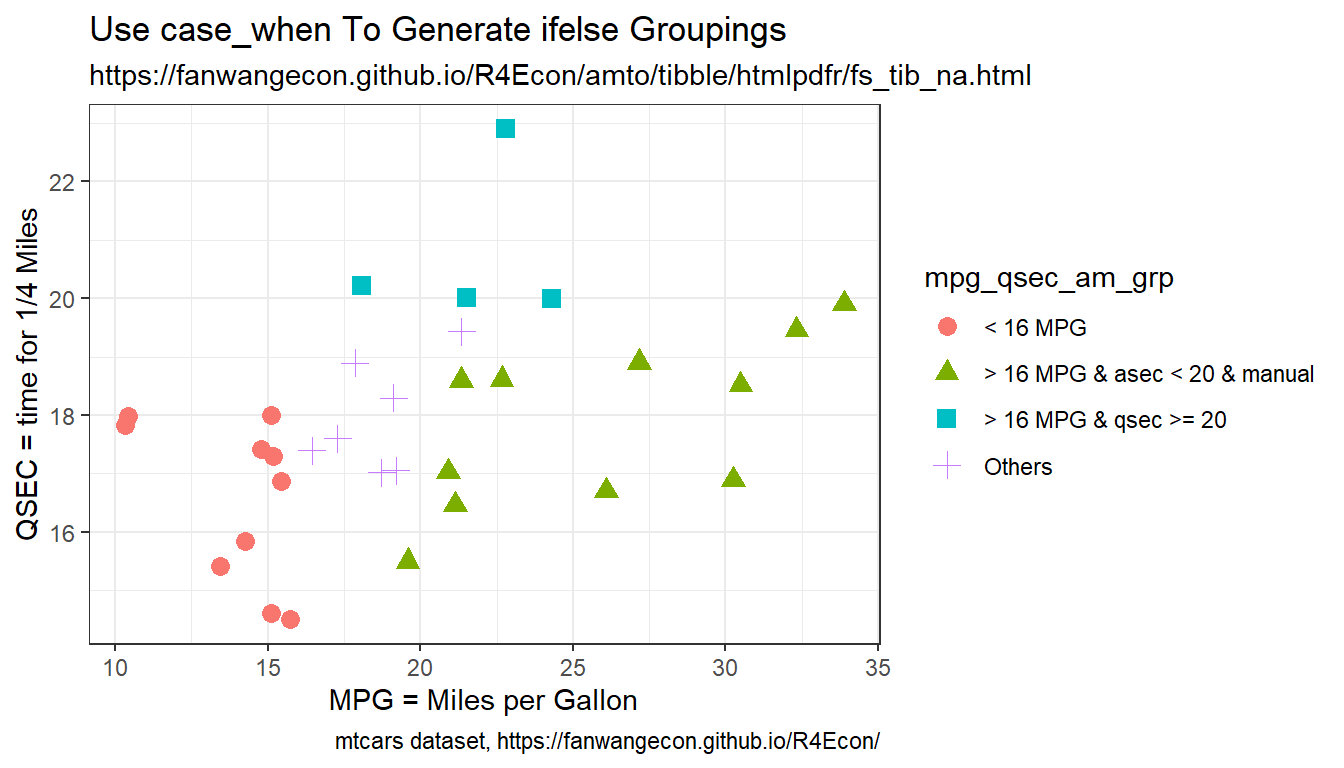
\includegraphics{Panel-Data-and-Optimization-with-R_files/figure-latex/unnamed-chunk-101-1} \end{center}

\begin{Shaded}
\begin{Highlighting}[]
\FunctionTok{ggplot}\NormalTok{(tb\_test\_data, }\FunctionTok{aes}\NormalTok{(}\AttributeTok{x=}\NormalTok{exam\_score)) }\SpecialCharTok{+}
  \FunctionTok{geom\_histogram}\NormalTok{(}\AttributeTok{bins=}\DecValTok{16}\NormalTok{) }\SpecialCharTok{+}
  \FunctionTok{labs}\NormalTok{(}\AttributeTok{title =} \FunctionTok{paste0}\NormalTok{(}\StringTok{\textquotesingle{}Exam Distribution\textquotesingle{}}\NormalTok{),}
       \AttributeTok{caption =} \StringTok{\textquotesingle{}All Sections\textquotesingle{}}\NormalTok{) }\SpecialCharTok{+}
  \FunctionTok{theme\_bw}\NormalTok{()}
\end{Highlighting}
\end{Shaded}

\begin{center}\includegraphics{Panel-Data-and-Optimization-with-R_files/figure-latex/unnamed-chunk-102-1} \end{center}

\hypertarget{summarize-multiple-variables}{%
\section{Summarize Multiple Variables}\label{summarize-multiple-variables}}

\hypertarget{generate-replace-variables}{%
\subsection{Generate Replace Variables}\label{generate-replace-variables}}

\begin{quote}
Go back to \href{http://fanwangecon.github.io/}{fan}'s \href{https://fanwangecon.github.io/REconTools/}{REconTools} Package, \href{https://fanwangecon.github.io/R4Econ/}{R Code Examples} Repository (\href{https://fanwangecon.github.io/R4Econ/bookdown}{bookdown site}), or \href{https://fanwangecon.github.io/Stat4Econ/}{Intro Stats with R} Repository (\href{https://fanwangecon.github.io/Stat4Econ/bookdown}{bookdown site}).
\end{quote}

\hypertarget{replace-na-for-multiple-variables}{%
\subsubsection{Replace NA for Multiple Variables}\label{replace-na-for-multiple-variables}}

Replace some variables NA by some values, and other variables' NAs by other values.

\begin{Shaded}
\begin{Highlighting}[]
\CommentTok{\# Define}
\NormalTok{it\_N }\OtherTok{\textless{}{-}} \DecValTok{3}
\NormalTok{it\_M }\OtherTok{\textless{}{-}} \DecValTok{5}
\NormalTok{svr\_id }\OtherTok{\textless{}{-}} \StringTok{\textquotesingle{}date\textquotesingle{}}

\CommentTok{\# NA dataframe}
\NormalTok{df\_NA }\OtherTok{\textless{}{-}} \FunctionTok{as\_tibble}\NormalTok{(}\FunctionTok{matrix}\NormalTok{(}\ConstantTok{NA}\NormalTok{, }\AttributeTok{nrow=}\NormalTok{it\_N, }\AttributeTok{ncol=}\NormalTok{it\_M)) }\SpecialCharTok{\%\textgreater{}\%}
  \FunctionTok{rowid\_to\_column}\NormalTok{(}\AttributeTok{var =}\NormalTok{ svr\_id) }\SpecialCharTok{\%\textgreater{}\%}
  \FunctionTok{rename\_at}\NormalTok{(}\FunctionTok{vars}\NormalTok{(}\FunctionTok{starts\_with}\NormalTok{(}\StringTok{"V"}\NormalTok{)),}
            \FunctionTok{funs}\NormalTok{(}\FunctionTok{str\_replace}\NormalTok{(., }\StringTok{"V"}\NormalTok{, }\StringTok{"var"}\NormalTok{)))}
\FunctionTok{kable}\NormalTok{(df\_NA) }\SpecialCharTok{\%\textgreater{}\%}
  \FunctionTok{kable\_styling\_fc}\NormalTok{()}
\end{Highlighting}
\end{Shaded}

\begin{table}[!h]
\centering
\begin{tabular}{r|l|l|l|l|l}
\hline
date & var1 & var2 & var3 & var4 & var5\\
\hline
\cellcolor{gray!6}{1} & \cellcolor{gray!6}{NA} & \cellcolor{gray!6}{NA} & \cellcolor{gray!6}{NA} & \cellcolor{gray!6}{NA} & \cellcolor{gray!6}{NA}\\
\hline
2 & NA & NA & NA & NA & NA\\
\hline
\cellcolor{gray!6}{3} & \cellcolor{gray!6}{NA} & \cellcolor{gray!6}{NA} & \cellcolor{gray!6}{NA} & \cellcolor{gray!6}{NA} & \cellcolor{gray!6}{NA}\\
\hline
\end{tabular}
\end{table}

\begin{Shaded}
\begin{Highlighting}[]
\CommentTok{\# Replace NA}
\NormalTok{df\_NA\_replace }\OtherTok{\textless{}{-}}\NormalTok{ df\_NA }\SpecialCharTok{\%\textgreater{}\%}
  \FunctionTok{mutate\_at}\NormalTok{(}\FunctionTok{vars}\NormalTok{(}\FunctionTok{one\_of}\NormalTok{(}\FunctionTok{c}\NormalTok{(}\StringTok{\textquotesingle{}var1\textquotesingle{}}\NormalTok{, }\StringTok{\textquotesingle{}var2\textquotesingle{}}\NormalTok{))), }\FunctionTok{list}\NormalTok{(}\SpecialCharTok{\textasciitilde{}}\FunctionTok{replace\_na}\NormalTok{(., }\DecValTok{0}\NormalTok{))) }\SpecialCharTok{\%\textgreater{}\%}
  \FunctionTok{mutate\_at}\NormalTok{(}\FunctionTok{vars}\NormalTok{(}\FunctionTok{one\_of}\NormalTok{(}\FunctionTok{c}\NormalTok{(}\StringTok{\textquotesingle{}var3\textquotesingle{}}\NormalTok{, }\StringTok{\textquotesingle{}var5\textquotesingle{}}\NormalTok{))), }\FunctionTok{list}\NormalTok{(}\SpecialCharTok{\textasciitilde{}}\FunctionTok{replace\_na}\NormalTok{(., }\DecValTok{99}\NormalTok{)))}
\FunctionTok{kable}\NormalTok{(df\_NA\_replace) }\SpecialCharTok{\%\textgreater{}\%}
  \FunctionTok{kable\_styling\_fc}\NormalTok{()}
\end{Highlighting}
\end{Shaded}

\begin{table}[!h]
\centering
\begin{tabular}{r|r|r|r|l|r}
\hline
date & var1 & var2 & var3 & var4 & var5\\
\hline
\cellcolor{gray!6}{1} & \cellcolor{gray!6}{0} & \cellcolor{gray!6}{0} & \cellcolor{gray!6}{99} & \cellcolor{gray!6}{NA} & \cellcolor{gray!6}{99}\\
\hline
2 & 0 & 0 & 99 & NA & 99\\
\hline
\cellcolor{gray!6}{3} & \cellcolor{gray!6}{0} & \cellcolor{gray!6}{0} & \cellcolor{gray!6}{99} & \cellcolor{gray!6}{NA} & \cellcolor{gray!6}{99}\\
\hline
\end{tabular}
\end{table}

\hypertarget{cumulative-sum-multiple-variables}{%
\subsubsection{Cumulative Sum Multiple Variables}\label{cumulative-sum-multiple-variables}}

Each row is a different date, each column is the profit a firms earns on a date, we want to compute cumulatively how much a person is earning. Also renames variable names below jointly.

\begin{Shaded}
\begin{Highlighting}[]
\CommentTok{\# Define}
\NormalTok{it\_N }\OtherTok{\textless{}{-}} \DecValTok{3}
\NormalTok{it\_M }\OtherTok{\textless{}{-}} \DecValTok{5}
\NormalTok{svr\_id }\OtherTok{\textless{}{-}} \StringTok{\textquotesingle{}date\textquotesingle{}}

\CommentTok{\# random dataframe, daily profit of firms}
\CommentTok{\# dp\_fx: daily profit firm ID something}
\FunctionTok{set.seed}\NormalTok{(}\DecValTok{123}\NormalTok{)}
\NormalTok{df\_daily\_profit }\OtherTok{\textless{}{-}} \FunctionTok{as\_tibble}\NormalTok{(}\FunctionTok{matrix}\NormalTok{(}\FunctionTok{rnorm}\NormalTok{(it\_N}\SpecialCharTok{*}\NormalTok{it\_M), }\AttributeTok{nrow=}\NormalTok{it\_N, }\AttributeTok{ncol=}\NormalTok{it\_M)) }\SpecialCharTok{\%\textgreater{}\%}
  \FunctionTok{rowid\_to\_column}\NormalTok{(}\AttributeTok{var =}\NormalTok{ svr\_id) }\SpecialCharTok{\%\textgreater{}\%}
  \FunctionTok{rename\_at}\NormalTok{(}\FunctionTok{vars}\NormalTok{(}\FunctionTok{starts\_with}\NormalTok{(}\StringTok{"V"}\NormalTok{)),}
            \FunctionTok{funs}\NormalTok{(}\FunctionTok{str\_replace}\NormalTok{(., }\StringTok{"V"}\NormalTok{, }\StringTok{"dp\_f"}\NormalTok{)))}
\FunctionTok{kable}\NormalTok{(df\_daily\_profit) }\SpecialCharTok{\%\textgreater{}\%}
  \FunctionTok{kable\_styling\_fc}\NormalTok{()}
\end{Highlighting}
\end{Shaded}

\begin{table}[!h]
\centering
\begin{tabular}{r|r|r|r|r|r}
\hline
date & dp\_f1 & dp\_f2 & dp\_f3 & dp\_f4 & dp\_f5\\
\hline
\cellcolor{gray!6}{1} & \cellcolor{gray!6}{-0.5604756} & \cellcolor{gray!6}{0.0705084} & \cellcolor{gray!6}{0.4609162} & \cellcolor{gray!6}{-0.4456620} & \cellcolor{gray!6}{0.4007715}\\
\hline
2 & -0.2301775 & 0.1292877 & -1.2650612 & 1.2240818 & 0.1106827\\
\hline
\cellcolor{gray!6}{3} & \cellcolor{gray!6}{1.5587083} & \cellcolor{gray!6}{1.7150650} & \cellcolor{gray!6}{-0.6868529} & \cellcolor{gray!6}{0.3598138} & \cellcolor{gray!6}{-0.5558411}\\
\hline
\end{tabular}
\end{table}

\begin{Shaded}
\begin{Highlighting}[]
\CommentTok{\# cumulative sum with suffix}
\NormalTok{df\_cumu\_profit\_suffix }\OtherTok{\textless{}{-}}\NormalTok{ df\_daily\_profit }\SpecialCharTok{\%\textgreater{}\%}
  \FunctionTok{mutate\_at}\NormalTok{(}\FunctionTok{vars}\NormalTok{(}\FunctionTok{contains}\NormalTok{(}\StringTok{\textquotesingle{}dp\_f\textquotesingle{}}\NormalTok{)), }\AttributeTok{.funs =} \FunctionTok{list}\NormalTok{(}\AttributeTok{cumu =} \SpecialCharTok{\textasciitilde{}}\FunctionTok{cumsum}\NormalTok{(.)))}
\FunctionTok{kable}\NormalTok{(df\_cumu\_profit\_suffix) }\SpecialCharTok{\%\textgreater{}\%}
  \FunctionTok{kable\_styling\_fc\_wide}\NormalTok{()}
\end{Highlighting}
\end{Shaded}

\begin{table}[!h]
\centering
\resizebox{\linewidth}{!}{
\begin{tabular}{r|r|r|r|r|r|r|r|r|r|r}
\hline
date & dp\_f1 & dp\_f2 & dp\_f3 & dp\_f4 & dp\_f5 & dp\_f1\_cumu & dp\_f2\_cumu & dp\_f3\_cumu & dp\_f4\_cumu & dp\_f5\_cumu\\
\hline
\cellcolor{gray!6}{1} & \cellcolor{gray!6}{-0.5604756} & \cellcolor{gray!6}{0.0705084} & \cellcolor{gray!6}{0.4609162} & \cellcolor{gray!6}{-0.4456620} & \cellcolor{gray!6}{0.4007715} & \cellcolor{gray!6}{-0.5604756} & \cellcolor{gray!6}{0.0705084} & \cellcolor{gray!6}{0.4609162} & \cellcolor{gray!6}{-0.4456620} & \cellcolor{gray!6}{0.4007715}\\
\hline
2 & -0.2301775 & 0.1292877 & -1.2650612 & 1.2240818 & 0.1106827 & -0.7906531 & 0.1997961 & -0.8041450 & 0.7784198 & 0.5114542\\
\hline
\cellcolor{gray!6}{3} & \cellcolor{gray!6}{1.5587083} & \cellcolor{gray!6}{1.7150650} & \cellcolor{gray!6}{-0.6868529} & \cellcolor{gray!6}{0.3598138} & \cellcolor{gray!6}{-0.5558411} & \cellcolor{gray!6}{0.7680552} & \cellcolor{gray!6}{1.9148611} & \cellcolor{gray!6}{-1.4909979} & \cellcolor{gray!6}{1.1382337} & \cellcolor{gray!6}{-0.0443870}\\
\hline
\end{tabular}}
\end{table}

\begin{Shaded}
\begin{Highlighting}[]
\CommentTok{\# cumulative sum variables naming to prefix}
\NormalTok{df\_cumu\_profit }\OtherTok{\textless{}{-}}\NormalTok{ df\_cumu\_profit\_suffix }\SpecialCharTok{\%\textgreater{}\%}
  \FunctionTok{rename\_at}\NormalTok{(}\FunctionTok{vars}\NormalTok{(}\FunctionTok{contains}\NormalTok{( }\StringTok{"\_cumu"}\NormalTok{) ), }\FunctionTok{list}\NormalTok{(}\SpecialCharTok{\textasciitilde{}}\FunctionTok{paste}\NormalTok{(}\StringTok{"cp\_f"}\NormalTok{, }\FunctionTok{gsub}\NormalTok{(}\StringTok{"\_cumu"}\NormalTok{, }\StringTok{""}\NormalTok{, .), }\AttributeTok{sep =} \StringTok{""}\NormalTok{))) }\SpecialCharTok{\%\textgreater{}\%}
  \FunctionTok{rename\_at}\NormalTok{(}\FunctionTok{vars}\NormalTok{(}\FunctionTok{contains}\NormalTok{( }\StringTok{"cp\_f"}\NormalTok{) ), }\FunctionTok{list}\NormalTok{(}\SpecialCharTok{\textasciitilde{}}\FunctionTok{gsub}\NormalTok{(}\StringTok{"dp\_f"}\NormalTok{, }\StringTok{""}\NormalTok{, .)))}
\FunctionTok{kable}\NormalTok{(df\_cumu\_profit) }\SpecialCharTok{\%\textgreater{}\%}
  \FunctionTok{kable\_styling\_fc\_wide}\NormalTok{()}
\end{Highlighting}
\end{Shaded}

\begin{table}[!h]
\centering
\resizebox{\linewidth}{!}{
\begin{tabular}{r|r|r|r|r|r|r|r|r|r|r}
\hline
date & dp\_f1 & dp\_f2 & dp\_f3 & dp\_f4 & dp\_f5 & cp\_f1 & cp\_f2 & cp\_f3 & cp\_f4 & cp\_f5\\
\hline
\cellcolor{gray!6}{1} & \cellcolor{gray!6}{-0.5604756} & \cellcolor{gray!6}{0.0705084} & \cellcolor{gray!6}{0.4609162} & \cellcolor{gray!6}{-0.4456620} & \cellcolor{gray!6}{0.4007715} & \cellcolor{gray!6}{-0.5604756} & \cellcolor{gray!6}{0.0705084} & \cellcolor{gray!6}{0.4609162} & \cellcolor{gray!6}{-0.4456620} & \cellcolor{gray!6}{0.4007715}\\
\hline
2 & -0.2301775 & 0.1292877 & -1.2650612 & 1.2240818 & 0.1106827 & -0.7906531 & 0.1997961 & -0.8041450 & 0.7784198 & 0.5114542\\
\hline
\cellcolor{gray!6}{3} & \cellcolor{gray!6}{1.5587083} & \cellcolor{gray!6}{1.7150650} & \cellcolor{gray!6}{-0.6868529} & \cellcolor{gray!6}{0.3598138} & \cellcolor{gray!6}{-0.5558411} & \cellcolor{gray!6}{0.7680552} & \cellcolor{gray!6}{1.9148611} & \cellcolor{gray!6}{-1.4909979} & \cellcolor{gray!6}{1.1382337} & \cellcolor{gray!6}{-0.0443870}\\
\hline
\end{tabular}}
\end{table}

\hypertarget{functions}{%
\chapter{Functions}\label{functions}}

\hypertarget{dataframe-mutate}{%
\section{Dataframe Mutate}\label{dataframe-mutate}}

\hypertarget{row-input-functions}{%
\subsection{Row Input Functions}\label{row-input-functions}}

\begin{quote}
Go back to \href{http://fanwangecon.github.io/}{fan}'s \href{https://fanwangecon.github.io/REconTools/}{REconTools} Package, \href{https://fanwangecon.github.io/R4Econ/}{R Code Examples} Repository (\href{https://fanwangecon.github.io/R4Econ/bookdown}{bookdown site}), or \href{https://fanwangecon.github.io/Stat4Econ/}{Intro Stats with R} Repository (\href{https://fanwangecon.github.io/Stat4Econ/bookdown}{bookdown site}).
\end{quote}

We want evaluate nonlinear function f(Q\_i, y\_i, ar\_x, ar\_y, c, d), where c and d are constants, and ar\_x and ar\_y are arrays, both fixed. x\_i and y\_i vary over each row of matrix. We would like to evaluate this nonlinear function concurrently across \(N\) individuals. The eventual goal is to find the \(i\) specific \(Q\) that solves the nonlinear equations.

This is a continuation of \href{https://fanwangecon.github.io/R4Econ/function/noloop/fs_applysapplymutate.html}{R use Apply, Sapply and dplyr Mutate to Evaluate one Function Across Rows of a Matrix}

\hypertarget{set-up-input-arrays}{%
\subsubsection{Set up Input Arrays}\label{set-up-input-arrays}}

There is a function that takes \(M=Q+P\) inputs, we want to evaluate this function \(N\) times. Each time, there are \(M\) inputs, where all but \(Q\) of the \(M\) inputs, meaning \(P\) of the \(M\) inputs, are the same. In particular, \(P=Q*N\).

\[M = Q+P = Q + Q*N\]

\begin{Shaded}
\begin{Highlighting}[]
\CommentTok{\# it\_child\_count = N, the number of children}
\NormalTok{it\_N\_child\_cnt }\OtherTok{=} \DecValTok{5}
\CommentTok{\# it\_heter\_param = Q, number of parameters that are heterogeneous across children}
\NormalTok{it\_Q\_hetpa\_cnt }\OtherTok{=} \DecValTok{2}

\CommentTok{\# P fixed parameters, nN is N dimensional, nP is P dimensional}
\NormalTok{ar\_nN\_A }\OtherTok{=} \FunctionTok{seq}\NormalTok{(}\SpecialCharTok{{-}}\DecValTok{2}\NormalTok{, }\DecValTok{2}\NormalTok{, }\AttributeTok{length.out =}\NormalTok{ it\_N\_child\_cnt)}
\NormalTok{ar\_nN\_alpha }\OtherTok{=} \FunctionTok{seq}\NormalTok{(}\FloatTok{0.1}\NormalTok{, }\FloatTok{0.9}\NormalTok{, }\AttributeTok{length.out =}\NormalTok{ it\_N\_child\_cnt)}
\NormalTok{ar\_nP\_A\_alpha }\OtherTok{=} \FunctionTok{c}\NormalTok{(ar\_nN\_A, ar\_nN\_alpha)}
\NormalTok{ar\_nN\_N\_choice }\OtherTok{=} \FunctionTok{seq}\NormalTok{(}\DecValTok{1}\NormalTok{,it\_N\_child\_cnt)}\SpecialCharTok{/}\FunctionTok{sum}\NormalTok{(}\FunctionTok{seq}\NormalTok{(}\DecValTok{1}\NormalTok{,it\_N\_child\_cnt))}

\CommentTok{\# N by Q varying parameters}
\NormalTok{mt\_nN\_by\_nQ\_A\_alpha }\OtherTok{=} \FunctionTok{cbind}\NormalTok{(ar\_nN\_A, ar\_nN\_alpha, ar\_nN\_N\_choice)}

\CommentTok{\# Convert Matrix to Tibble}
\NormalTok{ar\_st\_col\_names }\OtherTok{=} \FunctionTok{c}\NormalTok{(}\StringTok{\textquotesingle{}fl\_A\textquotesingle{}}\NormalTok{, }\StringTok{\textquotesingle{}fl\_alpha\textquotesingle{}}\NormalTok{, }\StringTok{\textquotesingle{}fl\_N\textquotesingle{}}\NormalTok{)}
\NormalTok{tb\_nN\_by\_nQ\_A\_alpha }\OtherTok{\textless{}{-}} \FunctionTok{as\_tibble}\NormalTok{(mt\_nN\_by\_nQ\_A\_alpha) }\SpecialCharTok{\%\textgreater{}\%} \FunctionTok{rename\_all}\NormalTok{(}\SpecialCharTok{\textasciitilde{}}\FunctionTok{c}\NormalTok{(ar\_st\_col\_names))}

\CommentTok{\# Show}
\FunctionTok{kable}\NormalTok{(tb\_nN\_by\_nQ\_A\_alpha) }\SpecialCharTok{\%\textgreater{}\%}
  \FunctionTok{kable\_styling\_fc}\NormalTok{()}
\end{Highlighting}
\end{Shaded}

\begin{table}[!h]
\centering
\begin{tabular}{r|r|r}
\hline
fl\_A & fl\_alpha & fl\_N\\
\hline
\cellcolor{gray!6}{-2} & \cellcolor{gray!6}{0.1} & \cellcolor{gray!6}{0.0666667}\\
\hline
-1 & 0.3 & 0.1333333\\
\hline
\cellcolor{gray!6}{0} & \cellcolor{gray!6}{0.5} & \cellcolor{gray!6}{0.2000000}\\
\hline
1 & 0.7 & 0.2666667\\
\hline
\cellcolor{gray!6}{2} & \cellcolor{gray!6}{0.9} & \cellcolor{gray!6}{0.3333333}\\
\hline
\end{tabular}
\end{table}

\hypertarget{mutate-over-simple-function}{%
\subsubsection{Mutate over Simple Function}\label{mutate-over-simple-function}}

For this example, use a very simple function with only one type of input, all inputs are scalars.

\begin{Shaded}
\begin{Highlighting}[]
\CommentTok{\# Define Implicit Function}
\NormalTok{ffi\_nonlinear }\OtherTok{\textless{}{-}} \ControlFlowTok{function}\NormalTok{(fl\_A, fl\_alpha)\{}

\NormalTok{  fl\_out }\OtherTok{\textless{}{-}}\NormalTok{ (fl\_A }\SpecialCharTok{+}\NormalTok{ fl\_alpha}\SpecialCharTok{*}\NormalTok{fl\_A)}\SpecialCharTok{/}\NormalTok{(fl\_A)}\SpecialCharTok{\^{}}\DecValTok{2}

  \FunctionTok{return}\NormalTok{(fl\_out)}
\NormalTok{\}}
\end{Highlighting}
\end{Shaded}

Apply the function over the dataframe, note five different ways below, the third way allows for parameters to be strings.

\begin{Shaded}
\begin{Highlighting}[]
\CommentTok{\# variable names}
\NormalTok{svr\_fl\_A }\OtherTok{\textless{}{-}} \StringTok{\textquotesingle{}fl\_A\textquotesingle{}}
\NormalTok{svr\_fl\_alpha }\OtherTok{\textless{}{-}} \StringTok{\textquotesingle{}fl\_alpha\textquotesingle{}}

\CommentTok{\# Evaluate}
\NormalTok{tb\_nN\_by\_nQ\_A\_alpha\_mutate\_rows }\OtherTok{\textless{}{-}}\NormalTok{ tb\_nN\_by\_nQ\_A\_alpha }\SpecialCharTok{\%\textgreater{}\%}
  \FunctionTok{mutate}\NormalTok{(}\AttributeTok{fl\_out\_m1 =} \FunctionTok{ffi\_nonlinear}\NormalTok{(}\AttributeTok{fl\_A=}\NormalTok{.}\SpecialCharTok{$}\NormalTok{fl\_A, }\AttributeTok{fl\_alpha=}\NormalTok{.}\SpecialCharTok{$}\NormalTok{fl\_alpha),}
         \AttributeTok{fl\_out\_m2 =} \FunctionTok{ffi\_nonlinear}\NormalTok{(}\AttributeTok{fl\_A=}\StringTok{\textasciigrave{}}\AttributeTok{$}\StringTok{\textasciigrave{}}\NormalTok{(., }\StringTok{\textquotesingle{}fl\_A\textquotesingle{}}\NormalTok{), }\AttributeTok{fl\_alpha=}\StringTok{\textasciigrave{}}\AttributeTok{$}\StringTok{\textasciigrave{}}\NormalTok{(., }\StringTok{\textquotesingle{}fl\_alpha\textquotesingle{}}\NormalTok{)),}
         \AttributeTok{fl\_out\_m3 =} \FunctionTok{ffi\_nonlinear}\NormalTok{(}\AttributeTok{fl\_A=}\NormalTok{.[[svr\_fl\_A]], }\AttributeTok{fl\_alpha=}\NormalTok{.[[svr\_fl\_alpha]]),}
         \AttributeTok{fl\_out\_m4 =} \FunctionTok{ffi\_nonlinear}\NormalTok{(}\AttributeTok{fl\_A=}\NormalTok{fl\_A, }\AttributeTok{fl\_alpha=}\NormalTok{fl\_alpha),}
         \AttributeTok{fl\_out\_m5 =} \FunctionTok{ffi\_nonlinear}\NormalTok{(fl\_A, fl\_alpha))}

\CommentTok{\# print}
\FunctionTok{kable}\NormalTok{(tb\_nN\_by\_nQ\_A\_alpha\_mutate\_rows) }\SpecialCharTok{\%\textgreater{}\%} \FunctionTok{kable\_styling\_fc}\NormalTok{()}
\end{Highlighting}
\end{Shaded}

\begin{table}[!h]
\centering
\begin{tabular}{r|r|r|r|r|r|r|r}
\hline
fl\_A & fl\_alpha & fl\_N & fl\_out\_m1 & fl\_out\_m2 & fl\_out\_m3 & fl\_out\_m4 & fl\_out\_m5\\
\hline
\cellcolor{gray!6}{-2} & \cellcolor{gray!6}{0.1} & \cellcolor{gray!6}{0.0666667} & \cellcolor{gray!6}{-0.55} & \cellcolor{gray!6}{-0.55} & \cellcolor{gray!6}{-0.55} & \cellcolor{gray!6}{-0.55} & \cellcolor{gray!6}{-0.55}\\
\hline
-1 & 0.3 & 0.1333333 & -1.30 & -1.30 & -1.30 & -1.30 & -1.30\\
\hline
\cellcolor{gray!6}{0} & \cellcolor{gray!6}{0.5} & \cellcolor{gray!6}{0.2000000} & \cellcolor{gray!6}{NaN} & \cellcolor{gray!6}{NaN} & \cellcolor{gray!6}{NaN} & \cellcolor{gray!6}{NaN} & \cellcolor{gray!6}{NaN}\\
\hline
1 & 0.7 & 0.2666667 & 1.70 & 1.70 & 1.70 & 1.70 & 1.70\\
\hline
\cellcolor{gray!6}{2} & \cellcolor{gray!6}{0.9} & \cellcolor{gray!6}{0.3333333} & \cellcolor{gray!6}{0.95} & \cellcolor{gray!6}{0.95} & \cellcolor{gray!6}{0.95} & \cellcolor{gray!6}{0.95} & \cellcolor{gray!6}{0.95}\\
\hline
\end{tabular}
\end{table}

\hypertarget{testing-function-with-scalar-and-arrays}{%
\subsubsection{Testing Function with Scalar and Arrays}\label{testing-function-with-scalar-and-arrays}}

Test non-linear Equation.

\begin{Shaded}
\begin{Highlighting}[]
\CommentTok{\# Test Parameters}
\NormalTok{fl\_N\_agg }\OtherTok{=} \DecValTok{100}
\NormalTok{fl\_rho }\OtherTok{=} \SpecialCharTok{{-}}\DecValTok{1}
\NormalTok{fl\_N\_q }\OtherTok{=}\NormalTok{ ar\_nN\_N\_choice[}\DecValTok{4}\NormalTok{]}\SpecialCharTok{*}\NormalTok{fl\_N\_agg}
\NormalTok{ar\_A\_alpha }\OtherTok{=}\NormalTok{ mt\_nN\_by\_nQ\_A\_alpha[}\DecValTok{4}\NormalTok{,]}
\CommentTok{\# Apply Function}
\NormalTok{ar\_p1\_s1 }\OtherTok{=} \FunctionTok{exp}\NormalTok{((ar\_A\_alpha[}\DecValTok{1}\NormalTok{] }\SpecialCharTok{{-}}\NormalTok{ ar\_nN\_A)}\SpecialCharTok{*}\NormalTok{fl\_rho)}
\NormalTok{ar\_p1\_s2 }\OtherTok{=}\NormalTok{ (ar\_A\_alpha[}\DecValTok{2}\NormalTok{]}\SpecialCharTok{/}\NormalTok{ar\_nN\_alpha)}
\NormalTok{ar\_p1\_s3 }\OtherTok{=}\NormalTok{ (}\DecValTok{1}\SpecialCharTok{/}\NormalTok{(ar\_nN\_alpha}\SpecialCharTok{*}\NormalTok{fl\_rho }\SpecialCharTok{{-}} \DecValTok{1}\NormalTok{))}
\NormalTok{ar\_p1 }\OtherTok{=}\NormalTok{ (ar\_p1\_s1}\SpecialCharTok{*}\NormalTok{ar\_p1\_s2)}\SpecialCharTok{\^{}}\NormalTok{ar\_p1\_s3}
\NormalTok{ar\_p2 }\OtherTok{=}\NormalTok{ fl\_N\_q}\SpecialCharTok{\^{}}\NormalTok{((ar\_A\_alpha[}\DecValTok{2}\NormalTok{]}\SpecialCharTok{*}\NormalTok{fl\_rho}\DecValTok{{-}1}\NormalTok{)}\SpecialCharTok{/}\NormalTok{(ar\_nN\_alpha}\SpecialCharTok{*}\NormalTok{fl\_rho}\DecValTok{{-}1}\NormalTok{))}
\NormalTok{ar\_overall }\OtherTok{=}\NormalTok{ ar\_p1}\SpecialCharTok{*}\NormalTok{ar\_p2}
\NormalTok{fl\_overall }\OtherTok{=}\NormalTok{ fl\_N\_agg }\SpecialCharTok{{-}} \FunctionTok{sum}\NormalTok{(ar\_overall)}
\FunctionTok{print}\NormalTok{(fl\_overall)}
\end{Highlighting}
\end{Shaded}

\begin{verbatim}
## [1] -598.2559
\end{verbatim}

Implement the non-linear problem's evaluation using apply over all \(N\) individuals.

\begin{Shaded}
\begin{Highlighting}[]
\CommentTok{\# Define Implicit Function}
\NormalTok{ffi\_nonlin\_dplyrdo }\OtherTok{\textless{}{-}} \ControlFlowTok{function}\NormalTok{(fl\_A, fl\_alpha, fl\_N, ar\_A, ar\_alpha, fl\_N\_agg, fl\_rho)\{}
  \CommentTok{\# ar\_A\_alpha[1] is A}
  \CommentTok{\# ar\_A\_alpha[2] is alpha}

  \CommentTok{\# \# Test Parameters}
  \CommentTok{\# fl\_N = 100}
  \CommentTok{\# fl\_rho = {-}1}
  \CommentTok{\# fl\_N\_q = 10}

  \CommentTok{\# Apply Function}
\NormalTok{  ar\_p1\_s1 }\OtherTok{=} \FunctionTok{exp}\NormalTok{((fl\_A }\SpecialCharTok{{-}}\NormalTok{ ar\_A)}\SpecialCharTok{*}\NormalTok{fl\_rho)}
\NormalTok{  ar\_p1\_s2 }\OtherTok{=}\NormalTok{ (fl\_alpha}\SpecialCharTok{/}\NormalTok{ar\_alpha)}
\NormalTok{  ar\_p1\_s3 }\OtherTok{=}\NormalTok{ (}\DecValTok{1}\SpecialCharTok{/}\NormalTok{(ar\_alpha}\SpecialCharTok{*}\NormalTok{fl\_rho }\SpecialCharTok{{-}} \DecValTok{1}\NormalTok{))}
\NormalTok{  ar\_p1 }\OtherTok{=}\NormalTok{ (ar\_p1\_s1}\SpecialCharTok{*}\NormalTok{ar\_p1\_s2)}\SpecialCharTok{\^{}}\NormalTok{ar\_p1\_s3}
\NormalTok{  ar\_p2 }\OtherTok{=}\NormalTok{ fl\_N}\SpecialCharTok{\^{}}\NormalTok{((fl\_alpha}\SpecialCharTok{*}\NormalTok{fl\_rho}\DecValTok{{-}1}\NormalTok{)}\SpecialCharTok{/}\NormalTok{(ar\_alpha}\SpecialCharTok{*}\NormalTok{fl\_rho}\DecValTok{{-}1}\NormalTok{))}
\NormalTok{  ar\_overall }\OtherTok{=}\NormalTok{ ar\_p1}\SpecialCharTok{*}\NormalTok{ar\_p2}
\NormalTok{  fl\_overall }\OtherTok{=}\NormalTok{ fl\_N\_agg }\SpecialCharTok{{-}} \FunctionTok{sum}\NormalTok{(ar\_overall)}

  \FunctionTok{return}\NormalTok{(fl\_overall)}
\NormalTok{\}}

\CommentTok{\# Parameters}
\NormalTok{fl\_rho }\OtherTok{=} \SpecialCharTok{{-}}\DecValTok{1}

\CommentTok{\# Evaluate Function}
\FunctionTok{print}\NormalTok{(}\FunctionTok{ffi\_nonlin\_dplyrdo}\NormalTok{(mt\_nN\_by\_nQ\_A\_alpha[}\DecValTok{1}\NormalTok{,}\DecValTok{1}\NormalTok{],}
\NormalTok{                         mt\_nN\_by\_nQ\_A\_alpha[}\DecValTok{1}\NormalTok{,}\DecValTok{2}\NormalTok{],}
\NormalTok{                         mt\_nN\_by\_nQ\_A\_alpha[}\DecValTok{1}\NormalTok{,}\DecValTok{3}\NormalTok{]}\SpecialCharTok{*}\NormalTok{fl\_N\_agg,}
\NormalTok{                         ar\_nN\_A, ar\_nN\_alpha, fl\_N\_agg, fl\_rho))}
\end{Highlighting}
\end{Shaded}

\begin{verbatim}
## [1] 81.86645
\end{verbatim}

\begin{Shaded}
\begin{Highlighting}[]
\ControlFlowTok{for}\NormalTok{ (i }\ControlFlowTok{in} \FunctionTok{seq}\NormalTok{(}\DecValTok{1}\NormalTok{,}\FunctionTok{dim}\NormalTok{(mt\_nN\_by\_nQ\_A\_alpha)[}\DecValTok{1}\NormalTok{]))\{}
\NormalTok{  fl\_eval }\OtherTok{=} \FunctionTok{ffi\_nonlin\_dplyrdo}\NormalTok{(mt\_nN\_by\_nQ\_A\_alpha[i,}\DecValTok{1}\NormalTok{],}
\NormalTok{                               mt\_nN\_by\_nQ\_A\_alpha[i,}\DecValTok{2}\NormalTok{],}
\NormalTok{                               mt\_nN\_by\_nQ\_A\_alpha[i,}\DecValTok{3}\NormalTok{]}\SpecialCharTok{*}\NormalTok{fl\_N\_agg,}
\NormalTok{                               ar\_nN\_A, ar\_nN\_alpha, fl\_N\_agg, fl\_rho)}
  \FunctionTok{print}\NormalTok{(fl\_eval)}
\NormalTok{\}}
\end{Highlighting}
\end{Shaded}

\begin{verbatim}
## [1] 81.86645
## [1] 54.48885
## [1] -65.5619
## [1] -598.2559
## [1] -3154.072
\end{verbatim}

\hypertarget{evaluate-nonlinear-function-using-dplyr-mutate}{%
\subsubsection{Evaluate Nonlinear Function using dplyr mutate}\label{evaluate-nonlinear-function-using-dplyr-mutate}}

\begin{Shaded}
\begin{Highlighting}[]
\CommentTok{\# Define Implicit Function}
\NormalTok{ffi\_nonlin\_dplyrdo }\OtherTok{\textless{}{-}} \ControlFlowTok{function}\NormalTok{(fl\_A, fl\_alpha, fl\_N, ar\_A, ar\_alpha, fl\_N\_agg, fl\_rho)\{}

  \CommentTok{\# Test Parameters}
  \CommentTok{\# ar\_A = ar\_nN\_A}
  \CommentTok{\# ar\_alpha = ar\_nN\_alpha}
  \CommentTok{\# fl\_N = 100}
  \CommentTok{\# fl\_rho = {-}1}
  \CommentTok{\# fl\_N\_q = 10}

  \CommentTok{\# Apply Function}
\NormalTok{  ar\_p1\_s1 }\OtherTok{=} \FunctionTok{exp}\NormalTok{((fl\_A }\SpecialCharTok{{-}}\NormalTok{ ar\_A)}\SpecialCharTok{*}\NormalTok{fl\_rho)}
\NormalTok{  ar\_p1\_s2 }\OtherTok{=}\NormalTok{ (fl\_alpha}\SpecialCharTok{/}\NormalTok{ar\_alpha)}
\NormalTok{  ar\_p1\_s3 }\OtherTok{=}\NormalTok{ (}\DecValTok{1}\SpecialCharTok{/}\NormalTok{(ar\_alpha}\SpecialCharTok{*}\NormalTok{fl\_rho }\SpecialCharTok{{-}} \DecValTok{1}\NormalTok{))}
\NormalTok{  ar\_p1 }\OtherTok{=}\NormalTok{ (ar\_p1\_s1}\SpecialCharTok{*}\NormalTok{ar\_p1\_s2)}\SpecialCharTok{\^{}}\NormalTok{ar\_p1\_s3}
\NormalTok{  ar\_p2 }\OtherTok{=}\NormalTok{ (fl\_N}\SpecialCharTok{*}\NormalTok{fl\_N\_agg)}\SpecialCharTok{\^{}}\NormalTok{((fl\_alpha}\SpecialCharTok{*}\NormalTok{fl\_rho}\DecValTok{{-}1}\NormalTok{)}\SpecialCharTok{/}\NormalTok{(ar\_alpha}\SpecialCharTok{*}\NormalTok{fl\_rho}\DecValTok{{-}1}\NormalTok{))}
\NormalTok{  ar\_overall }\OtherTok{=}\NormalTok{ ar\_p1}\SpecialCharTok{*}\NormalTok{ar\_p2}
\NormalTok{  fl\_overall }\OtherTok{=}\NormalTok{ fl\_N\_agg }\SpecialCharTok{{-}} \FunctionTok{sum}\NormalTok{(ar\_overall)}

  \FunctionTok{return}\NormalTok{(fl\_overall)}
\NormalTok{\}}

\CommentTok{\# fl\_A, fl\_alpha are from columns of tb\_nN\_by\_nQ\_A\_alpha}
\NormalTok{tb\_nN\_by\_nQ\_A\_alpha }\OtherTok{=}\NormalTok{ tb\_nN\_by\_nQ\_A\_alpha }\SpecialCharTok{\%\textgreater{}\%} \FunctionTok{rowwise}\NormalTok{() }\SpecialCharTok{\%\textgreater{}\%}
                        \FunctionTok{mutate}\NormalTok{(}\AttributeTok{dplyr\_eval =} \FunctionTok{ffi\_nonlin\_dplyrdo}\NormalTok{(fl\_A, fl\_alpha, fl\_N,}
\NormalTok{                                                               ar\_nN\_A, ar\_nN\_alpha,}
\NormalTok{                                                               fl\_N\_agg, fl\_rho))}
\CommentTok{\# Show}
\FunctionTok{kable}\NormalTok{(tb\_nN\_by\_nQ\_A\_alpha) }\SpecialCharTok{\%\textgreater{}\%}
  \FunctionTok{kable\_styling\_fc}\NormalTok{()}
\end{Highlighting}
\end{Shaded}

\begin{table}[!h]
\centering
\begin{tabular}{r|r|r|r}
\hline
fl\_A & fl\_alpha & fl\_N & dplyr\_eval\\
\hline
\cellcolor{gray!6}{-2} & \cellcolor{gray!6}{0.1} & \cellcolor{gray!6}{0.0666667} & \cellcolor{gray!6}{81.86645}\\
\hline
-1 & 0.3 & 0.1333333 & 54.48885\\
\hline
\cellcolor{gray!6}{0} & \cellcolor{gray!6}{0.5} & \cellcolor{gray!6}{0.2000000} & \cellcolor{gray!6}{-65.56190}\\
\hline
1 & 0.7 & 0.2666667 & -598.25595\\
\hline
\cellcolor{gray!6}{2} & \cellcolor{gray!6}{0.9} & \cellcolor{gray!6}{0.3333333} & \cellcolor{gray!6}{-3154.07226}\\
\hline
\end{tabular}
\end{table}

\hypertarget{evaluate-choices-across-states}{%
\subsection{Evaluate Choices Across States}\label{evaluate-choices-across-states}}

\begin{quote}
Go back to \href{http://fanwangecon.github.io/}{fan}'s \href{https://fanwangecon.github.io/REconTools/}{REconTools} Package, \href{https://fanwangecon.github.io/R4Econ/}{R Code Examples} Repository (\href{https://fanwangecon.github.io/R4Econ/bookdown}{bookdown site}), or \href{https://fanwangecon.github.io/Stat4Econ/}{Intro Stats with R} Repository (\href{https://fanwangecon.github.io/Stat4Econ/bookdown}{bookdown site}).
\end{quote}

See the \href{https://fanwangecon.github.io/REconTools/reference/ff_opti_bisect_pmap_multi.html}{ff\_opti\_bisect\_pmap\_multi} function from \href{https://fanwangecon.github.io/}{Fan}'s \emph{\href{https://fanwangecon.github.io/REconTools/}{REconTools}} Package, which provides a resuable function based on the algorithm worked out here.

We want evaluate linear function \(0=f(z_{ij}, x_i, y_i, \textbf{X}, \textbf{Y}, c, d)\). There are \(i\) functions that have \(i\) specific \(x\) and \(y\). For each \(i\) function, we evaluate along a grid of feasible values for \(z\), over \(j\in J\) grid points, potentially looking for the \(j\) that is closest to the root. \(\textbf{X}\) and \(\textbf{Y}\) are arrays common across the \(i\) equations, and \(c\) and \(d\) are constants.

The evaluation strategy is the following, given min and max for \(z\) that are specific for each \(j\), and given common number of grid points, generate a matrix of \(z_{ij}\). Suppose there the number of \(i\) is \(I\), and the number of grid points for \(j\) is \(J\).

\begin{enumerate}
\def\labelenumi{\arabic{enumi}.}
\tightlist
\item
  Generate a \(J \cdot I\) by \(3\) matrix where the columns are \(z,x,y\) as tibble
\item
  Follow \href{https://fanwangecon.github.io/R4Econ/function/mutatef/fs_funceval.html}{this} Mutate to evaluate the \(f(\cdot)\) function.
\item
  Add two categorical columns for grid levels and wich \(i\), \(i\) and \(j\) index. Plot Mutate output evaluated column categorized by \(i\) as color and \(j\) as x-axis.
\end{enumerate}

\hypertarget{set-up-input-arrays-1}{%
\subsubsection{Set up Input Arrays}\label{set-up-input-arrays-1}}

There is a function that takes \(M=Q+P\) inputs, we want to evaluate this function \(N\) times. Each time, there are \(M\) inputs, where all but \(Q\) of the \(M\) inputs, meaning \(P\) of the \(M\) inputs, are the same. In particular, \(P=Q*N\).

\[M = Q+P = Q + Q*N\]

Now we need to expand this by the number of choice grid. Each row, representing one equation, is expanded by the number of choice grids. We are graphically searching, or rather brute force searching, which means if we have 100 individuals, we want to plot out the nonlinear equation for each of these lines, and show graphically where each line crosses zero. We achieve this, by evaluating the equation for each of the 100 individuals along a grid of feasible choices.

In this problem here, the feasible choices are shared across individuals.

\begin{Shaded}
\begin{Highlighting}[]
\CommentTok{\# Parameters}
\NormalTok{fl\_rho }\OtherTok{=} \FloatTok{0.20}
\NormalTok{svr\_id\_var }\OtherTok{=} \StringTok{\textquotesingle{}INDI\_ID\textquotesingle{}}

\CommentTok{\# it\_child\_count = N, the number of children}
\NormalTok{it\_N\_child\_cnt }\OtherTok{=} \DecValTok{4}
\CommentTok{\# it\_heter\_param = Q, number of parameters that are heterogeneous across children}
\NormalTok{it\_Q\_hetpa\_cnt }\OtherTok{=} \DecValTok{2}

\CommentTok{\# P fixed parameters, nN is N dimensional, nP is P dimensional}
\NormalTok{ar\_nN\_A }\OtherTok{=} \FunctionTok{seq}\NormalTok{(}\SpecialCharTok{{-}}\DecValTok{2}\NormalTok{, }\DecValTok{2}\NormalTok{, }\AttributeTok{length.out =}\NormalTok{ it\_N\_child\_cnt)}
\NormalTok{ar\_nN\_alpha }\OtherTok{=} \FunctionTok{seq}\NormalTok{(}\FloatTok{0.1}\NormalTok{, }\FloatTok{0.9}\NormalTok{, }\AttributeTok{length.out =}\NormalTok{ it\_N\_child\_cnt)}
\NormalTok{ar\_nP\_A\_alpha }\OtherTok{=} \FunctionTok{c}\NormalTok{(ar\_nN\_A, ar\_nN\_alpha)}

\CommentTok{\# N by Q varying parameters}
\NormalTok{mt\_nN\_by\_nQ\_A\_alpha }\OtherTok{=} \FunctionTok{cbind}\NormalTok{(ar\_nN\_A, ar\_nN\_alpha)}

\CommentTok{\# Choice Grid for nutritional feasible choices for each}
\NormalTok{fl\_N\_agg }\OtherTok{=} \DecValTok{100}
\NormalTok{fl\_N\_min }\OtherTok{=} \DecValTok{0}
\NormalTok{it\_N\_choice\_cnt\_ttest }\OtherTok{=} \DecValTok{3}
\NormalTok{it\_N\_choice\_cnt\_dense }\OtherTok{=} \DecValTok{100}
\NormalTok{ar\_N\_choices\_ttest }\OtherTok{=} \FunctionTok{seq}\NormalTok{(fl\_N\_min, fl\_N\_agg, }\AttributeTok{length.out =}\NormalTok{ it\_N\_choice\_cnt\_ttest)}
\NormalTok{ar\_N\_choices\_dense }\OtherTok{=} \FunctionTok{seq}\NormalTok{(fl\_N\_min, fl\_N\_agg, }\AttributeTok{length.out =}\NormalTok{ it\_N\_choice\_cnt\_dense)}

\CommentTok{\# Mesh Expand}
\NormalTok{tb\_states\_choices }\OtherTok{\textless{}{-}} \FunctionTok{as\_tibble}\NormalTok{(mt\_nN\_by\_nQ\_A\_alpha) }\SpecialCharTok{\%\textgreater{}\%} \FunctionTok{rowid\_to\_column}\NormalTok{(}\AttributeTok{var=}\NormalTok{svr\_id\_var)}
\NormalTok{tb\_states\_choices\_ttest }\OtherTok{\textless{}{-}}\NormalTok{ tb\_states\_choices }\SpecialCharTok{\%\textgreater{}\%} \FunctionTok{expand\_grid}\NormalTok{(}\AttributeTok{choices =}\NormalTok{ ar\_N\_choices\_ttest)}
\NormalTok{tb\_states\_choices\_dense }\OtherTok{\textless{}{-}}\NormalTok{ tb\_states\_choices }\SpecialCharTok{\%\textgreater{}\%} \FunctionTok{expand\_grid}\NormalTok{(}\AttributeTok{choices =}\NormalTok{ ar\_N\_choices\_dense)}

\CommentTok{\# display}
\FunctionTok{summary}\NormalTok{(tb\_states\_choices\_dense)}
\end{Highlighting}
\end{Shaded}

\begin{verbatim}
##     INDI_ID        ar_nN_A    ar_nN_alpha     choices   
##  Min.   :1.00   Min.   :-2   Min.   :0.1   Min.   :  0  
##  1st Qu.:1.75   1st Qu.:-1   1st Qu.:0.3   1st Qu.: 25  
##  Median :2.50   Median : 0   Median :0.5   Median : 50  
##  Mean   :2.50   Mean   : 0   Mean   :0.5   Mean   : 50  
##  3rd Qu.:3.25   3rd Qu.: 1   3rd Qu.:0.7   3rd Qu.: 75  
##  Max.   :4.00   Max.   : 2   Max.   :0.9   Max.   :100
\end{verbatim}

\begin{Shaded}
\begin{Highlighting}[]
\FunctionTok{kable}\NormalTok{(tb\_states\_choices\_ttest) }\SpecialCharTok{\%\textgreater{}\%}
  \FunctionTok{kable\_styling\_fc}\NormalTok{()}
\end{Highlighting}
\end{Shaded}

\begin{table}[!h]
\centering
\begin{tabular}{r|r|r|r}
\hline
INDI\_ID & ar\_nN\_A & ar\_nN\_alpha & choices\\
\hline
\cellcolor{gray!6}{1} & \cellcolor{gray!6}{-2.0000000} & \cellcolor{gray!6}{0.1000000} & \cellcolor{gray!6}{0}\\
\hline
1 & -2.0000000 & 0.1000000 & 50\\
\hline
\cellcolor{gray!6}{1} & \cellcolor{gray!6}{-2.0000000} & \cellcolor{gray!6}{0.1000000} & \cellcolor{gray!6}{100}\\
\hline
2 & -0.6666667 & 0.3666667 & 0\\
\hline
\cellcolor{gray!6}{2} & \cellcolor{gray!6}{-0.6666667} & \cellcolor{gray!6}{0.3666667} & \cellcolor{gray!6}{50}\\
\hline
2 & -0.6666667 & 0.3666667 & 100\\
\hline
\cellcolor{gray!6}{3} & \cellcolor{gray!6}{0.6666667} & \cellcolor{gray!6}{0.6333333} & \cellcolor{gray!6}{0}\\
\hline
3 & 0.6666667 & 0.6333333 & 50\\
\hline
\cellcolor{gray!6}{3} & \cellcolor{gray!6}{0.6666667} & \cellcolor{gray!6}{0.6333333} & \cellcolor{gray!6}{100}\\
\hline
4 & 2.0000000 & 0.9000000 & 0\\
\hline
\cellcolor{gray!6}{4} & \cellcolor{gray!6}{2.0000000} & \cellcolor{gray!6}{0.9000000} & \cellcolor{gray!6}{50}\\
\hline
4 & 2.0000000 & 0.9000000 & 100\\
\hline
\end{tabular}
\end{table}

\hypertarget{apply-same-function-all-rows-some-inputs-row-specific-other-shared}{%
\subsubsection{Apply Same Function all Rows, Some Inputs Row-specific, other Shared}\label{apply-same-function-all-rows-some-inputs-row-specific-other-shared}}

There are two types of inputs, row-specific inputs, and inputs that should be applied for each row. The Function just requires all of these inputs, it does not know what is row-specific and what is common for all row. Dplyr recognizes which parameter inputs already existing in the piped dataframe/tibble, given rowwise, those will be row-specific inputs. Additional function parameters that do not exist in dataframe as variable names, but that are pre-defined scalars or arrays will be applied to all rows.

\begin{itemize}
\tightlist
\item
  \citet{param} string variable name of input where functions are evaluated, these are already contained in the dataframe, existing variable names, row specific, rowwise computation over these, each rowwise calculation using different rows: \emph{fl\_A}, \emph{fl\_alpha}, \emph{fl\_N}
\item
  \citet{param} scalar and array values that are applied to every rowwise calculation, all rowwise calculations using the same scalars and arrays:\emph{ar\_A}, \emph{ar\_alpha}, \emph{fl\_N\_agg}, \emph{fl\_rho}
\item
  \citet{param} string output variable name
\end{itemize}

The function looks within group, finds min/max etc that are relevant.

\hypertarget{points-and-denser-dataframs-and-define-function}{%
\paragraph{3 Points and Denser Dataframs and Define Function}\label{points-and-denser-dataframs-and-define-function}}

\begin{Shaded}
\begin{Highlighting}[]
\CommentTok{\# Convert Matrix to Tibble}
\NormalTok{ar\_st\_col\_names }\OtherTok{=} \FunctionTok{c}\NormalTok{(svr\_id\_var,}\StringTok{\textquotesingle{}fl\_A\textquotesingle{}}\NormalTok{, }\StringTok{\textquotesingle{}fl\_alpha\textquotesingle{}}\NormalTok{)}
\NormalTok{tb\_states\_choices }\OtherTok{\textless{}{-}}\NormalTok{ tb\_states\_choices }\SpecialCharTok{\%\textgreater{}\%} \FunctionTok{rename\_all}\NormalTok{(}\SpecialCharTok{\textasciitilde{}}\FunctionTok{c}\NormalTok{(ar\_st\_col\_names))}
\NormalTok{ar\_st\_col\_names }\OtherTok{=} \FunctionTok{c}\NormalTok{(svr\_id\_var,}\StringTok{\textquotesingle{}fl\_A\textquotesingle{}}\NormalTok{, }\StringTok{\textquotesingle{}fl\_alpha\textquotesingle{}}\NormalTok{, }\StringTok{\textquotesingle{}fl\_N\textquotesingle{}}\NormalTok{)}
\NormalTok{tb\_states\_choices\_ttest }\OtherTok{\textless{}{-}}\NormalTok{ tb\_states\_choices\_ttest }\SpecialCharTok{\%\textgreater{}\%} \FunctionTok{rename\_all}\NormalTok{(}\SpecialCharTok{\textasciitilde{}}\FunctionTok{c}\NormalTok{(ar\_st\_col\_names))}
\NormalTok{tb\_states\_choices\_dense }\OtherTok{\textless{}{-}}\NormalTok{ tb\_states\_choices\_dense }\SpecialCharTok{\%\textgreater{}\%} \FunctionTok{rename\_all}\NormalTok{(}\SpecialCharTok{\textasciitilde{}}\FunctionTok{c}\NormalTok{(ar\_st\_col\_names))}

\CommentTok{\# Define Implicit Function}
\NormalTok{ffi\_nonlin\_dplyrdo }\OtherTok{\textless{}{-}} \ControlFlowTok{function}\NormalTok{(fl\_A, fl\_alpha, fl\_N, ar\_A, ar\_alpha, fl\_N\_agg, fl\_rho)\{}
  \CommentTok{\# scalar value that are row{-}specific, in dataframe already: *fl\_A*, *fl\_alpha*, *fl\_N*}
  \CommentTok{\# array and scalars not in dataframe, common all rows: *ar\_A*, *ar\_alpha*, *fl\_N\_agg*, *fl\_rho*}

  \CommentTok{\# Test Parameters}
  \CommentTok{\# ar\_A = ar\_nN\_A}
  \CommentTok{\# ar\_alpha = ar\_nN\_alpha}
  \CommentTok{\# fl\_N = 100}
  \CommentTok{\# fl\_rho = {-}1}
  \CommentTok{\# fl\_N\_q = 10}

  \CommentTok{\# Apply Function}
\NormalTok{  ar\_p1\_s1 }\OtherTok{=} \FunctionTok{exp}\NormalTok{((fl\_A }\SpecialCharTok{{-}}\NormalTok{ ar\_A)}\SpecialCharTok{*}\NormalTok{fl\_rho)}
\NormalTok{  ar\_p1\_s2 }\OtherTok{=}\NormalTok{ (fl\_alpha}\SpecialCharTok{/}\NormalTok{ar\_alpha)}
\NormalTok{  ar\_p1\_s3 }\OtherTok{=}\NormalTok{ (}\DecValTok{1}\SpecialCharTok{/}\NormalTok{(ar\_alpha}\SpecialCharTok{*}\NormalTok{fl\_rho }\SpecialCharTok{{-}} \DecValTok{1}\NormalTok{))}
\NormalTok{  ar\_p1 }\OtherTok{=}\NormalTok{ (ar\_p1\_s1}\SpecialCharTok{*}\NormalTok{ar\_p1\_s2)}\SpecialCharTok{\^{}}\NormalTok{ar\_p1\_s3}
\NormalTok{  ar\_p2 }\OtherTok{=}\NormalTok{ fl\_N}\SpecialCharTok{\^{}}\NormalTok{((fl\_alpha}\SpecialCharTok{*}\NormalTok{fl\_rho}\DecValTok{{-}1}\NormalTok{)}\SpecialCharTok{/}\NormalTok{(ar\_alpha}\SpecialCharTok{*}\NormalTok{fl\_rho}\DecValTok{{-}1}\NormalTok{))}
\NormalTok{  ar\_overall }\OtherTok{=}\NormalTok{ ar\_p1}\SpecialCharTok{*}\NormalTok{ar\_p2}
\NormalTok{  fl\_overall }\OtherTok{=}\NormalTok{ fl\_N\_agg }\SpecialCharTok{{-}} \FunctionTok{sum}\NormalTok{(ar\_overall)}

  \FunctionTok{return}\NormalTok{(fl\_overall)}
\NormalTok{\}}
\end{Highlighting}
\end{Shaded}

\hypertarget{evaluate-at-three-choice-points-and-show-table}{%
\paragraph{Evaluate at Three Choice Points and Show Table}\label{evaluate-at-three-choice-points-and-show-table}}

In the example below, just show results evaluating over three choice points and show table.

\begin{Shaded}
\begin{Highlighting}[]
\CommentTok{\# fl\_A, fl\_alpha are from columns of tb\_nN\_by\_nQ\_A\_alpha}
\NormalTok{tb\_states\_choices\_ttest\_eval }\OtherTok{=}\NormalTok{ tb\_states\_choices\_ttest }\SpecialCharTok{\%\textgreater{}\%} \FunctionTok{rowwise}\NormalTok{() }\SpecialCharTok{\%\textgreater{}\%}
                        \FunctionTok{mutate}\NormalTok{(}\AttributeTok{dplyr\_eval =} \FunctionTok{ffi\_nonlin\_dplyrdo}\NormalTok{(fl\_A, fl\_alpha, fl\_N,}
\NormalTok{                                                               ar\_nN\_A, ar\_nN\_alpha,}
\NormalTok{                                                               fl\_N\_agg, fl\_rho))}
\CommentTok{\# Show}
\FunctionTok{kable}\NormalTok{(tb\_states\_choices\_ttest\_eval) }\SpecialCharTok{\%\textgreater{}\%}
  \FunctionTok{kable\_styling\_fc}\NormalTok{()}
\end{Highlighting}
\end{Shaded}

\begin{table}[!h]
\centering
\begin{tabular}{r|r|r|r|r}
\hline
INDI\_ID & fl\_A & fl\_alpha & fl\_N & dplyr\_eval\\
\hline
\cellcolor{gray!6}{1} & \cellcolor{gray!6}{-2.0000000} & \cellcolor{gray!6}{0.1000000} & \cellcolor{gray!6}{0} & \cellcolor{gray!6}{100.00000}\\
\hline
1 & -2.0000000 & 0.1000000 & 50 & -5666.95576\\
\hline
\cellcolor{gray!6}{1} & \cellcolor{gray!6}{-2.0000000} & \cellcolor{gray!6}{0.1000000} & \cellcolor{gray!6}{100} & \cellcolor{gray!6}{-12880.28392}\\
\hline
2 & -0.6666667 & 0.3666667 & 0 & 100.00000\\
\hline
\cellcolor{gray!6}{2} & \cellcolor{gray!6}{-0.6666667} & \cellcolor{gray!6}{0.3666667} & \cellcolor{gray!6}{50} & \cellcolor{gray!6}{-595.73454}\\
\hline
2 & -0.6666667 & 0.3666667 & 100 & -1394.70698\\
\hline
\cellcolor{gray!6}{3} & \cellcolor{gray!6}{0.6666667} & \cellcolor{gray!6}{0.6333333} & \cellcolor{gray!6}{0} & \cellcolor{gray!6}{100.00000}\\
\hline
3 & 0.6666667 & 0.6333333 & 50 & -106.51058\\
\hline
\cellcolor{gray!6}{3} & \cellcolor{gray!6}{0.6666667} & \cellcolor{gray!6}{0.6333333} & \cellcolor{gray!6}{100} & \cellcolor{gray!6}{-323.94216}\\
\hline
4 & 2.0000000 & 0.9000000 & 0 & 100.00000\\
\hline
\cellcolor{gray!6}{4} & \cellcolor{gray!6}{2.0000000} & \cellcolor{gray!6}{0.9000000} & \cellcolor{gray!6}{50} & \cellcolor{gray!6}{22.55577}\\
\hline
4 & 2.0000000 & 0.9000000 & 100 & -51.97161\\
\hline
\end{tabular}
\end{table}

\hypertarget{evaluate-at-many-choice-points-and-show-graphically}{%
\paragraph{Evaluate at Many Choice Points and Show Graphically}\label{evaluate-at-many-choice-points-and-show-graphically}}

Same as above, but now we evaluate the function over the individuals at many choice points so that we can graph things out.

\begin{Shaded}
\begin{Highlighting}[]
\CommentTok{\# fl\_A, fl\_alpha are from columns of tb\_nN\_by\_nQ\_A\_alpha}
\NormalTok{tb\_states\_choices\_dense\_eval }\OtherTok{=}\NormalTok{ tb\_states\_choices\_dense }\SpecialCharTok{\%\textgreater{}\%} \FunctionTok{rowwise}\NormalTok{() }\SpecialCharTok{\%\textgreater{}\%}
                        \FunctionTok{mutate}\NormalTok{(}\AttributeTok{dplyr\_eval =} \FunctionTok{ffi\_nonlin\_dplyrdo}\NormalTok{(fl\_A, fl\_alpha, fl\_N,}
\NormalTok{                                                               ar\_nN\_A, ar\_nN\_alpha,}
\NormalTok{                                                               fl\_N\_agg, fl\_rho))}
\end{Highlighting}
\end{Shaded}

\begin{Shaded}
\begin{Highlighting}[]
\CommentTok{\# Labeling}
\NormalTok{st\_title }\OtherTok{\textless{}{-}} \FunctionTok{paste0}\NormalTok{(}\StringTok{\textquotesingle{}Evaluate Non{-}Linear Functions to Search for Roots\textquotesingle{}}\NormalTok{)}
\NormalTok{st\_subtitle }\OtherTok{\textless{}{-}} \FunctionTok{paste0}\NormalTok{(}\StringTok{\textquotesingle{}https://fanwangecon.github.io/\textquotesingle{}}\NormalTok{,}
                      \StringTok{\textquotesingle{}R4Econ/function/mutatef/htmlpdfr/fs\_func\_choice\_states.html\textquotesingle{}}\NormalTok{)}
\NormalTok{st\_caption }\OtherTok{\textless{}{-}} \FunctionTok{paste0}\NormalTok{(}\StringTok{\textquotesingle{}Evaluating the function, \textquotesingle{}}\NormalTok{,}
                     \StringTok{\textquotesingle{}https://fanwangecon.github.io/R4Econ/\textquotesingle{}}\NormalTok{)}
\NormalTok{st\_x\_label }\OtherTok{\textless{}{-}} \StringTok{\textquotesingle{}x values\textquotesingle{}}
\NormalTok{st\_y\_label }\OtherTok{\textless{}{-}} \StringTok{\textquotesingle{}f(x)\textquotesingle{}}

\CommentTok{\# Show}
\FunctionTok{dim}\NormalTok{(tb\_states\_choices\_dense\_eval)}
\end{Highlighting}
\end{Shaded}

\begin{verbatim}
## [1] 400   5
\end{verbatim}

\begin{Shaded}
\begin{Highlighting}[]
\FunctionTok{summary}\NormalTok{(tb\_states\_choices\_dense\_eval)}
\end{Highlighting}
\end{Shaded}

\begin{verbatim}
##     INDI_ID          fl_A       fl_alpha        fl_N       dplyr_eval       
##  Min.   :1.00   Min.   :-2   Min.   :0.1   Min.   :  0   Min.   :-12880.28  
##  1st Qu.:1.75   1st Qu.:-1   1st Qu.:0.3   1st Qu.: 25   1st Qu.: -1167.29  
##  Median :2.50   Median : 0   Median :0.5   Median : 50   Median :  -202.42  
##  Mean   :2.50   Mean   : 0   Mean   :0.5   Mean   : 50   Mean   : -1645.65  
##  3rd Qu.:3.25   3rd Qu.: 1   3rd Qu.:0.7   3rd Qu.: 75   3rd Qu.:     0.96  
##  Max.   :4.00   Max.   : 2   Max.   :0.9   Max.   :100   Max.   :   100.00
\end{verbatim}

\begin{Shaded}
\begin{Highlighting}[]
\NormalTok{lineplot }\OtherTok{\textless{}{-}}\NormalTok{ tb\_states\_choices\_dense\_eval }\SpecialCharTok{\%\textgreater{}\%}
    \FunctionTok{ggplot}\NormalTok{(}\FunctionTok{aes}\NormalTok{(}\AttributeTok{x=}\NormalTok{fl\_N, }\AttributeTok{y=}\NormalTok{dplyr\_eval)) }\SpecialCharTok{+}
        \FunctionTok{geom\_line}\NormalTok{() }\SpecialCharTok{+}
        \FunctionTok{facet\_wrap}\NormalTok{( . }\SpecialCharTok{\textasciitilde{}}\NormalTok{ INDI\_ID, }\AttributeTok{scales =} \StringTok{"free"}\NormalTok{) }\SpecialCharTok{+}
        \FunctionTok{geom\_hline}\NormalTok{(}\AttributeTok{yintercept=}\DecValTok{0}\NormalTok{, }\AttributeTok{linetype=}\StringTok{"dashed"}\NormalTok{,}
                \AttributeTok{color =} \StringTok{"red"}\NormalTok{, }\AttributeTok{size=}\DecValTok{1}\NormalTok{) }\SpecialCharTok{+}
        \FunctionTok{labs}\NormalTok{(}\AttributeTok{title =}\NormalTok{ st\_title,}
             \AttributeTok{subtitle =}\NormalTok{ st\_subtitle,}
             \AttributeTok{x =}\NormalTok{ st\_x\_label,}
             \AttributeTok{y =}\NormalTok{ st\_y\_label,}
             \AttributeTok{caption =}\NormalTok{ st\_caption)}
\FunctionTok{print}\NormalTok{(lineplot)}
\end{Highlighting}
\end{Shaded}

\begin{center}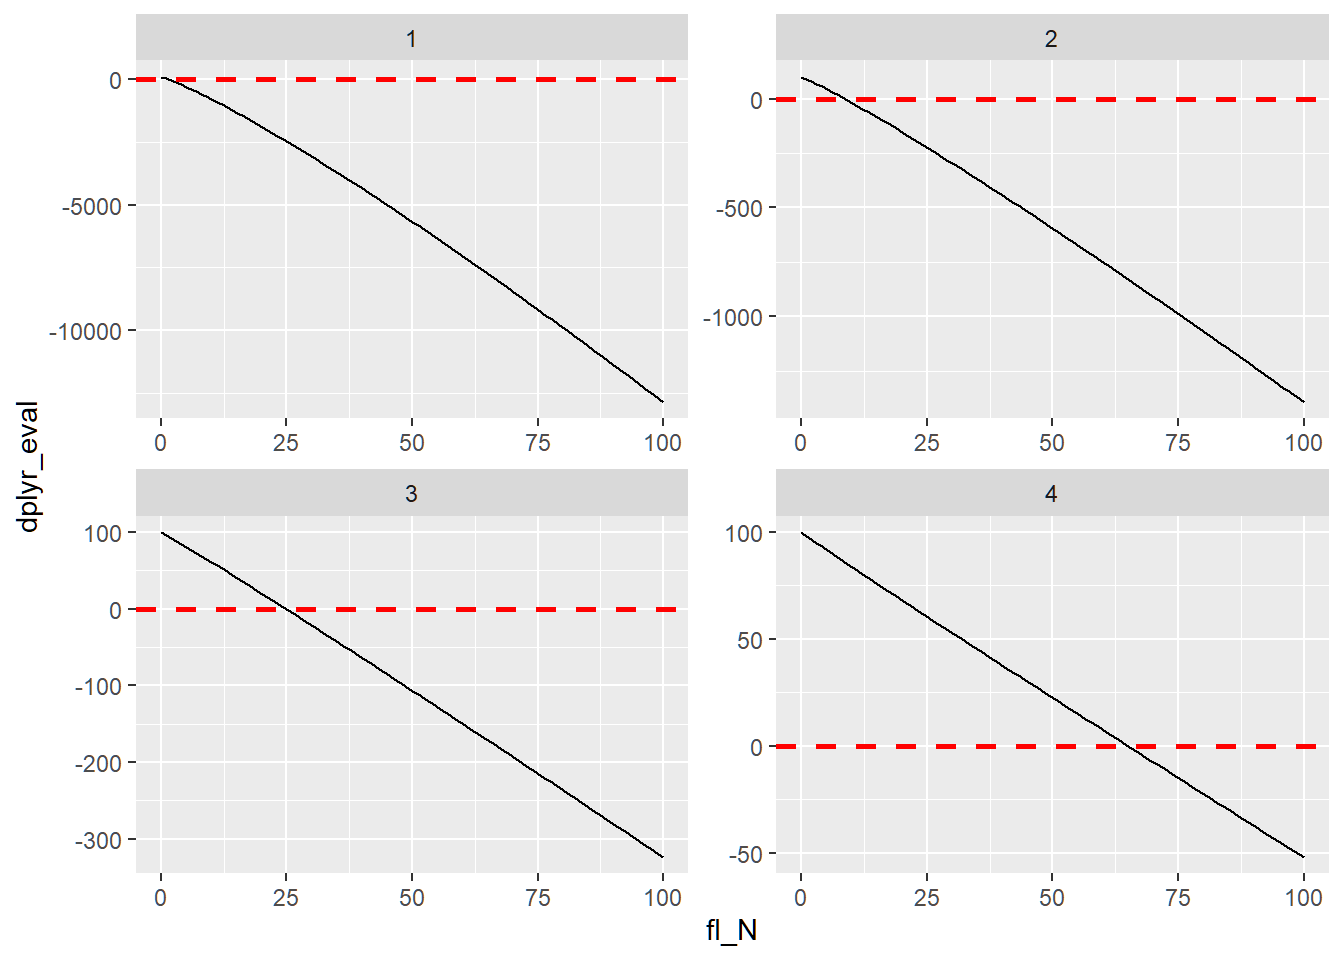
\includegraphics{Panel-Data-and-Optimization-with-R_files/figure-latex/graph many evaluations-1} \end{center}

\hypertarget{dataframe-do-anything}{%
\section{Dataframe Do Anything}\label{dataframe-do-anything}}

\hypertarget{mx1-by-n-to-mxq-by-n1}{%
\subsection{(Mx1 by N) to (MxQ by N+1)}\label{mx1-by-n-to-mxq-by-n1}}

\begin{quote}
Go back to \href{http://fanwangecon.github.io/}{fan}'s \href{https://fanwangecon.github.io/REconTools/}{REconTools} Package, \href{https://fanwangecon.github.io/R4Econ/}{R Code Examples} Repository (\href{https://fanwangecon.github.io/R4Econ/bookdown}{bookdown site}), or \href{https://fanwangecon.github.io/Stat4Econ/}{Intro Stats with R} Repository (\href{https://fanwangecon.github.io/Stat4Econ/bookdown}{bookdown site}).
\end{quote}

\textbf{Case One}: There is a dataframe with \(M\) rows, based on these \(m\) specific information, generate dataframes for each \(m\). Stack these indivdiual dataframes together and merge original \(m\) specific information in as well. The number of rows for each \(m\) is \(Q_m\), each \(m\) could have different number of expansion rows.

Generate a panel with \(M\) individuals, each individual is observed for different spans of times (\emph{uncount}). Before expanding, generate individual specific normal distribution standard deviation. All individuals share the same mean, but have increasing standard deviations.

\hypertarget{generate-dataframe-with-m-rows.}{%
\subsubsection{Generate Dataframe with M Rows.}\label{generate-dataframe-with-m-rows.}}

This is the first step, generate \(M\) rows of data, to be expanded. Each row contains the number of normal draws to make and the mean and the standard deviation for normal daraws that are \(m\) specific.

\begin{Shaded}
\begin{Highlighting}[]
\CommentTok{\# Parameter Setups}
\NormalTok{it\_M }\OtherTok{\textless{}{-}} \DecValTok{3}
\NormalTok{it\_Q\_max }\OtherTok{\textless{}{-}} \DecValTok{5}
\NormalTok{fl\_rnorm\_mu }\OtherTok{\textless{}{-}} \DecValTok{1000}
\NormalTok{ar\_rnorm\_sd }\OtherTok{\textless{}{-}} \FunctionTok{seq}\NormalTok{(}\FloatTok{0.01}\NormalTok{, }\DecValTok{200}\NormalTok{, }\AttributeTok{length.out=}\NormalTok{it\_M)}
\NormalTok{ar\_it\_q }\OtherTok{\textless{}{-}} \FunctionTok{sample.int}\NormalTok{(it\_Q\_max, it\_M, }\AttributeTok{replace=}\ConstantTok{TRUE}\NormalTok{)}

\CommentTok{\# N by Q varying parameters}
\NormalTok{mt\_data }\OtherTok{=} \FunctionTok{cbind}\NormalTok{(ar\_it\_q, ar\_rnorm\_sd)}
\NormalTok{tb\_M }\OtherTok{\textless{}{-}} \FunctionTok{as\_tibble}\NormalTok{(mt\_data) }\SpecialCharTok{\%\textgreater{}\%} \FunctionTok{rowid\_to\_column}\NormalTok{(}\AttributeTok{var =} \StringTok{"ID"}\NormalTok{) }\SpecialCharTok{\%\textgreater{}\%}
                \FunctionTok{rename}\NormalTok{(}\AttributeTok{sd =}\NormalTok{ ar\_rnorm\_sd, }\AttributeTok{Q =}\NormalTok{ ar\_it\_q) }\SpecialCharTok{\%\textgreater{}\%}
                \FunctionTok{mutate}\NormalTok{(}\AttributeTok{mean =}\NormalTok{ fl\_rnorm\_mu)}

\CommentTok{\# display}
\FunctionTok{kable}\NormalTok{(tb\_M) }\SpecialCharTok{\%\textgreater{}\%}
  \FunctionTok{kable\_styling\_fc}\NormalTok{()}
\end{Highlighting}
\end{Shaded}

\begin{table}[!h]
\centering
\begin{tabular}{r|r|r|r}
\hline
ID & Q & sd & mean\\
\hline
\cellcolor{gray!6}{1} & \cellcolor{gray!6}{1} & \cellcolor{gray!6}{0.010} & \cellcolor{gray!6}{1000}\\
\hline
2 & 3 & 100.005 & 1000\\
\hline
\cellcolor{gray!6}{3} & \cellcolor{gray!6}{4} & \cellcolor{gray!6}{200.000} & \cellcolor{gray!6}{1000}\\
\hline
\end{tabular}
\end{table}

\hypertarget{random-normal-draw-expansion}{%
\subsubsection{Random Normal Draw Expansion}\label{random-normal-draw-expansion}}

The steps are:

\begin{enumerate}
\def\labelenumi{\arabic{enumi}.}
\tightlist
\item
  \href{https://dplyr.tidyverse.org/reference/do.html}{do anything}
\item
  use ``.\$'' sign to refer to variable names, or {[}{[}`name'{]}{]}
\item
  unnest
\item
  left\_join expanded and original
\end{enumerate}

Note these all give the same results

Use dot dollar to get variables

\begin{Shaded}
\begin{Highlighting}[]
\CommentTok{\# Generate $Q\_m$ individual specific incomes, expanded different number of times for each m}
\NormalTok{tb\_income }\OtherTok{\textless{}{-}}\NormalTok{ tb\_M }\SpecialCharTok{\%\textgreater{}\%} \FunctionTok{group\_by}\NormalTok{(ID) }\SpecialCharTok{\%\textgreater{}\%}
  \FunctionTok{do}\NormalTok{(}\AttributeTok{income =} \FunctionTok{rnorm}\NormalTok{(.}\SpecialCharTok{$}\NormalTok{Q, }\AttributeTok{mean=}\NormalTok{.}\SpecialCharTok{$}\NormalTok{mean, }\AttributeTok{sd=}\NormalTok{.}\SpecialCharTok{$}\NormalTok{sd)) }\SpecialCharTok{\%\textgreater{}\%}
  \FunctionTok{unnest}\NormalTok{(}\FunctionTok{c}\NormalTok{(income))}

\CommentTok{\# Merge back with tb\_M}
\NormalTok{tb\_income\_full\_dd }\OtherTok{\textless{}{-}}\NormalTok{ tb\_income }\SpecialCharTok{\%\textgreater{}\%}
  \FunctionTok{left\_join}\NormalTok{(tb\_M)}

\CommentTok{\# display}
\FunctionTok{kable}\NormalTok{(tb\_income) }\SpecialCharTok{\%\textgreater{}\%}
  \FunctionTok{kable\_styling\_fc}\NormalTok{()}
\end{Highlighting}
\end{Shaded}

\begin{table}[!h]
\centering
\begin{tabular}{r|r}
\hline
ID & income\\
\hline
\cellcolor{gray!6}{1} & \cellcolor{gray!6}{999.9803}\\
\hline
2 & 1070.1391\\
\hline
\cellcolor{gray!6}{2} & \cellcolor{gray!6}{952.7185}\\
\hline
2 & 893.2123\\
\hline
\cellcolor{gray!6}{3} & \cellcolor{gray!6}{956.4050}\\
\hline
3 & 794.7991\\
\hline
\cellcolor{gray!6}{3} & \cellcolor{gray!6}{854.2218}\\
\hline
3 & 874.9921\\
\hline
\end{tabular}
\end{table}

\begin{Shaded}
\begin{Highlighting}[]
\FunctionTok{kable}\NormalTok{(tb\_income\_full\_dd) }\SpecialCharTok{\%\textgreater{}\%}
  \FunctionTok{kable\_styling\_fc}\NormalTok{()}
\end{Highlighting}
\end{Shaded}

\begin{table}[!h]
\centering
\begin{tabular}{r|r|r|r|r}
\hline
ID & income & Q & sd & mean\\
\hline
\cellcolor{gray!6}{1} & \cellcolor{gray!6}{999.9803} & \cellcolor{gray!6}{1} & \cellcolor{gray!6}{0.010} & \cellcolor{gray!6}{1000}\\
\hline
2 & 1070.1391 & 3 & 100.005 & 1000\\
\hline
\cellcolor{gray!6}{2} & \cellcolor{gray!6}{952.7185} & \cellcolor{gray!6}{3} & \cellcolor{gray!6}{100.005} & \cellcolor{gray!6}{1000}\\
\hline
2 & 893.2123 & 3 & 100.005 & 1000\\
\hline
\cellcolor{gray!6}{3} & \cellcolor{gray!6}{956.4050} & \cellcolor{gray!6}{4} & \cellcolor{gray!6}{200.000} & \cellcolor{gray!6}{1000}\\
\hline
3 & 794.7991 & 4 & 200.000 & 1000\\
\hline
\cellcolor{gray!6}{3} & \cellcolor{gray!6}{854.2218} & \cellcolor{gray!6}{4} & \cellcolor{gray!6}{200.000} & \cellcolor{gray!6}{1000}\\
\hline
3 & 874.9921 & 4 & 200.000 & 1000\\
\hline
\end{tabular}
\end{table}

\hypertarget{mxp-by-n-to-mx1-by-1}{%
\subsection{(MxP by N) to (Mx1 by 1)}\label{mxp-by-n-to-mx1-by-1}}

\begin{quote}
Go back to \href{http://fanwangecon.github.io/}{fan}'s \href{https://fanwangecon.github.io/REconTools/}{REconTools} Package, \href{https://fanwangecon.github.io/R4Econ/}{R Code Examples} Repository (\href{https://fanwangecon.github.io/R4Econ/bookdown}{bookdown site}), or \href{https://fanwangecon.github.io/Stat4Econ/}{Intro Stats with R} Repository (\href{https://fanwangecon.github.io/Stat4Econ/bookdown}{bookdown site}).
\end{quote}

There is a Panel with \(M\) individuals and each individual has \(Q\) records/rows. A function generate an individual specific outcome given the \(Q\) individual specific inputs, along with shared parameters and arrays across the \(M\) individuals.

For example, suppose we have a dataframe of individual wage information from different countries, each row is an individual from one country. We want to generate country specific gini based on the individual data for each country in the dataframe. But additionally, perhaps the gini formula requires not just individual income but some additional parameters or shared dataframes as inputs.

Given the within \(m\) income observations, we can compute gini statistics that are individual specific based on the observed distribution of incomes. For this, we will use the \href{https://fanwangecon.github.io/REconTools/reference/ff_dist_gini_vector_pos.html}{ff\_dist\_gini\_vector\_pos.html} function from \href{https://fanwangecon.github.io/REconTools/}{REconTools}.

To make this more interesting, we will generate large dataframe with more \(M\) and more \(Q\) each \(m\).

\hypertarget{income-rows-for-individuals-in-many-groups}{%
\subsubsection{Income Rows for Individuals in Many Groups}\label{income-rows-for-individuals-in-many-groups}}

There are up to ten thousand income observation per person. And there are ten people.

\begin{Shaded}
\begin{Highlighting}[]
\CommentTok{\# Parameter Setups}
\NormalTok{it\_M }\OtherTok{\textless{}{-}} \DecValTok{10}
\NormalTok{it\_Q\_max }\OtherTok{\textless{}{-}} \DecValTok{10000}
\NormalTok{fl\_rnorm\_mu }\OtherTok{\textless{}{-}} \DecValTok{1}
\NormalTok{ar\_rnorm\_sd }\OtherTok{\textless{}{-}} \FunctionTok{seq}\NormalTok{(}\FloatTok{0.01}\NormalTok{, }\FloatTok{0.2}\NormalTok{, }\AttributeTok{length.out=}\NormalTok{it\_M)}
\NormalTok{ar\_it\_q }\OtherTok{\textless{}{-}} \FunctionTok{sample.int}\NormalTok{(it\_Q\_max, it\_M, }\AttributeTok{replace=}\ConstantTok{TRUE}\NormalTok{)}

\CommentTok{\# N by Q varying parameters}
\NormalTok{mt\_data }\OtherTok{=} \FunctionTok{cbind}\NormalTok{(ar\_it\_q, ar\_rnorm\_sd)}
\NormalTok{tb\_M }\OtherTok{\textless{}{-}} \FunctionTok{as\_tibble}\NormalTok{(mt\_data) }\SpecialCharTok{\%\textgreater{}\%} \FunctionTok{rowid\_to\_column}\NormalTok{(}\AttributeTok{var =} \StringTok{"ID"}\NormalTok{) }\SpecialCharTok{\%\textgreater{}\%}
                \FunctionTok{rename}\NormalTok{(}\AttributeTok{sd =}\NormalTok{ ar\_rnorm\_sd, }\AttributeTok{Q =}\NormalTok{ ar\_it\_q) }\SpecialCharTok{\%\textgreater{}\%}
                \FunctionTok{mutate}\NormalTok{(}\AttributeTok{mean =}\NormalTok{ fl\_rnorm\_mu)}
\end{Highlighting}
\end{Shaded}

\hypertarget{compute-group-specific-gini}{%
\subsubsection{Compute Group Specific Gini}\label{compute-group-specific-gini}}

There is only one input for the gini function \emph{ar\_pos}. Note that the gini are not very large even with large SD, because these are normal distributions. By Construction, most peple are in the middle. So with almost zero standard deviation, we have perfect equality, as standard deviation increases, inequality increases, but still pretty equal overall, there is no fat upper tail.

Note that there are three ways of referring to variable names with dot, which are all shown below:

\begin{enumerate}
\def\labelenumi{\arabic{enumi}.}
\tightlist
\item
  We can explicitly refer to names
\item
  We can use the \href{https://stackoverflow.com/a/18228613/8280804}{dollar dot structure} to use string variable names in do anything.
\item
  We can use dot bracket, this is the only option that works with string variable names
\end{enumerate}

First: Generate individual group all incomes:

\begin{Shaded}
\begin{Highlighting}[]
\CommentTok{\# A. Normal Draw Expansion, Explicitly Name}
\FunctionTok{set.seed}\NormalTok{(}\StringTok{\textquotesingle{}123\textquotesingle{}}\NormalTok{)}
\NormalTok{tb\_income\_norm\_dot\_dollar }\OtherTok{\textless{}{-}}\NormalTok{ tb\_M }\SpecialCharTok{\%\textgreater{}\%} \FunctionTok{group\_by}\NormalTok{(ID) }\SpecialCharTok{\%\textgreater{}\%}
  \FunctionTok{do}\NormalTok{(}\AttributeTok{income =} \FunctionTok{rnorm}\NormalTok{(.}\SpecialCharTok{$}\NormalTok{Q,}
                    \AttributeTok{mean=}\NormalTok{.}\SpecialCharTok{$}\NormalTok{mean,}
                    \AttributeTok{sd=}\NormalTok{.}\SpecialCharTok{$}\NormalTok{sd)) }\SpecialCharTok{\%\textgreater{}\%}
  \FunctionTok{unnest}\NormalTok{(}\FunctionTok{c}\NormalTok{(income)) }\SpecialCharTok{\%\textgreater{}\%}
  \FunctionTok{left\_join}\NormalTok{(tb\_M, }\AttributeTok{by=}\StringTok{"ID"}\NormalTok{)}

\CommentTok{\# Normal Draw Expansion again, dot dollar differently with string variable name}
\FunctionTok{set.seed}\NormalTok{(}\StringTok{\textquotesingle{}123\textquotesingle{}}\NormalTok{)}
\NormalTok{tb\_income\_norm\_dollar\_dot }\OtherTok{\textless{}{-}}\NormalTok{ tb\_M }\SpecialCharTok{\%\textgreater{}\%} \FunctionTok{group\_by}\NormalTok{(ID) }\SpecialCharTok{\%\textgreater{}\%}
  \FunctionTok{do}\NormalTok{(}\AttributeTok{income =} \FunctionTok{rnorm}\NormalTok{(}\StringTok{\textasciigrave{}}\AttributeTok{$}\StringTok{\textasciigrave{}}\NormalTok{(., }\StringTok{\textquotesingle{}Q\textquotesingle{}}\NormalTok{),}
                    \AttributeTok{mean =} \StringTok{\textasciigrave{}}\AttributeTok{$}\StringTok{\textasciigrave{}}\NormalTok{(., }\StringTok{\textquotesingle{}mean\textquotesingle{}}\NormalTok{),}
                    \AttributeTok{sd =} \StringTok{\textasciigrave{}}\AttributeTok{$}\StringTok{\textasciigrave{}}\NormalTok{(., }\StringTok{\textquotesingle{}sd\textquotesingle{}}\NormalTok{))) }\SpecialCharTok{\%\textgreater{}\%}
  \FunctionTok{unnest}\NormalTok{(}\FunctionTok{c}\NormalTok{(income)) }\SpecialCharTok{\%\textgreater{}\%}
  \FunctionTok{left\_join}\NormalTok{(tb\_M, }\AttributeTok{by=}\StringTok{"ID"}\NormalTok{)}

\CommentTok{\# Normal Draw Expansion again, dot double bracket}
\FunctionTok{set.seed}\NormalTok{(}\StringTok{\textquotesingle{}123\textquotesingle{}}\NormalTok{)}
\NormalTok{svr\_mean }\OtherTok{\textless{}{-}} \StringTok{\textquotesingle{}mean\textquotesingle{}}
\NormalTok{svr\_sd }\OtherTok{\textless{}{-}} \StringTok{\textquotesingle{}sd\textquotesingle{}}
\NormalTok{svr\_Q }\OtherTok{\textless{}{-}} \StringTok{\textquotesingle{}Q\textquotesingle{}}
\NormalTok{tb\_income\_norm\_dot\_bracket\_db }\OtherTok{\textless{}{-}}\NormalTok{ tb\_M }\SpecialCharTok{\%\textgreater{}\%} \FunctionTok{group\_by}\NormalTok{(ID) }\SpecialCharTok{\%\textgreater{}\%}
  \FunctionTok{do}\NormalTok{(}\AttributeTok{income =} \FunctionTok{rnorm}\NormalTok{(.[[svr\_Q]],}
                    \AttributeTok{mean =}\NormalTok{ .[[svr\_mean]],}
                    \AttributeTok{sd =}\NormalTok{ .[[svr\_sd]])) }\SpecialCharTok{\%\textgreater{}\%}
  \FunctionTok{unnest}\NormalTok{(}\FunctionTok{c}\NormalTok{(income)) }\SpecialCharTok{\%\textgreater{}\%}
  \FunctionTok{left\_join}\NormalTok{(tb\_M, }\AttributeTok{by=}\StringTok{"ID"}\NormalTok{)}

\CommentTok{\# display}
\FunctionTok{print}\NormalTok{(}\FunctionTok{dim}\NormalTok{(tb\_income\_norm\_dot\_bracket\_db))}
\end{Highlighting}
\end{Shaded}

\begin{verbatim}
## [1] 59429     5
\end{verbatim}

\begin{Shaded}
\begin{Highlighting}[]
\FunctionTok{kable}\NormalTok{(}\FunctionTok{head}\NormalTok{(tb\_income\_norm\_dot\_bracket\_db, }\DecValTok{20}\NormalTok{)) }\SpecialCharTok{\%\textgreater{}\%} \FunctionTok{kable\_styling\_fc}\NormalTok{()}
\end{Highlighting}
\end{Shaded}

\begin{table}[!h]
\centering
\begin{tabular}{r|r|r|r|r}
\hline
ID & income & Q & sd & mean\\
\hline
\cellcolor{gray!6}{1} & \cellcolor{gray!6}{0.9943952} & \cellcolor{gray!6}{3004} & \cellcolor{gray!6}{0.01} & \cellcolor{gray!6}{1}\\
\hline
1 & 0.9976982 & 3004 & 0.01 & 1\\
\hline
\cellcolor{gray!6}{1} & \cellcolor{gray!6}{1.0155871} & \cellcolor{gray!6}{3004} & \cellcolor{gray!6}{0.01} & \cellcolor{gray!6}{1}\\
\hline
1 & 1.0007051 & 3004 & 0.01 & 1\\
\hline
\cellcolor{gray!6}{1} & \cellcolor{gray!6}{1.0012929} & \cellcolor{gray!6}{3004} & \cellcolor{gray!6}{0.01} & \cellcolor{gray!6}{1}\\
\hline
1 & 1.0171506 & 3004 & 0.01 & 1\\
\hline
\cellcolor{gray!6}{1} & \cellcolor{gray!6}{1.0046092} & \cellcolor{gray!6}{3004} & \cellcolor{gray!6}{0.01} & \cellcolor{gray!6}{1}\\
\hline
1 & 0.9873494 & 3004 & 0.01 & 1\\
\hline
\cellcolor{gray!6}{1} & \cellcolor{gray!6}{0.9931315} & \cellcolor{gray!6}{3004} & \cellcolor{gray!6}{0.01} & \cellcolor{gray!6}{1}\\
\hline
1 & 0.9955434 & 3004 & 0.01 & 1\\
\hline
\cellcolor{gray!6}{1} & \cellcolor{gray!6}{1.0122408} & \cellcolor{gray!6}{3004} & \cellcolor{gray!6}{0.01} & \cellcolor{gray!6}{1}\\
\hline
1 & 1.0035981 & 3004 & 0.01 & 1\\
\hline
\cellcolor{gray!6}{1} & \cellcolor{gray!6}{1.0040077} & \cellcolor{gray!6}{3004} & \cellcolor{gray!6}{0.01} & \cellcolor{gray!6}{1}\\
\hline
1 & 1.0011068 & 3004 & 0.01 & 1\\
\hline
\cellcolor{gray!6}{1} & \cellcolor{gray!6}{0.9944416} & \cellcolor{gray!6}{3004} & \cellcolor{gray!6}{0.01} & \cellcolor{gray!6}{1}\\
\hline
1 & 1.0178691 & 3004 & 0.01 & 1\\
\hline
\cellcolor{gray!6}{1} & \cellcolor{gray!6}{1.0049785} & \cellcolor{gray!6}{3004} & \cellcolor{gray!6}{0.01} & \cellcolor{gray!6}{1}\\
\hline
1 & 0.9803338 & 3004 & 0.01 & 1\\
\hline
\cellcolor{gray!6}{1} & \cellcolor{gray!6}{1.0070136} & \cellcolor{gray!6}{3004} & \cellcolor{gray!6}{0.01} & \cellcolor{gray!6}{1}\\
\hline
1 & 0.9952721 & 3004 & 0.01 & 1\\
\hline
\end{tabular}
\end{table}

Second, compute gini:

\begin{Shaded}
\begin{Highlighting}[]
\CommentTok{\# Gini by Group}
\NormalTok{tb\_gini\_norm }\OtherTok{\textless{}{-}}\NormalTok{ tb\_income\_norm\_dot\_bracket\_db }\SpecialCharTok{\%\textgreater{}\%} \FunctionTok{group\_by}\NormalTok{(ID) }\SpecialCharTok{\%\textgreater{}\%}
  \FunctionTok{do}\NormalTok{(}\AttributeTok{inc\_gini\_norm =} \FunctionTok{ff\_dist\_gini\_vector\_pos}\NormalTok{(.}\SpecialCharTok{$}\NormalTok{income)) }\SpecialCharTok{\%\textgreater{}\%}
  \FunctionTok{unnest}\NormalTok{(}\FunctionTok{c}\NormalTok{(inc\_gini\_norm)) }\SpecialCharTok{\%\textgreater{}\%}
  \FunctionTok{left\_join}\NormalTok{(tb\_M, }\AttributeTok{by=}\StringTok{"ID"}\NormalTok{)}

\CommentTok{\# display}
\FunctionTok{kable}\NormalTok{(tb\_gini\_norm) }\SpecialCharTok{\%\textgreater{}\%} \FunctionTok{kable\_styling\_fc}\NormalTok{()}
\end{Highlighting}
\end{Shaded}

\begin{table}[!h]
\centering
\begin{tabular}{r|r|r|r|r}
\hline
ID & inc\_gini\_norm & Q & sd & mean\\
\hline
\cellcolor{gray!6}{1} & \cellcolor{gray!6}{0.0056006} & \cellcolor{gray!6}{3004} & \cellcolor{gray!6}{0.0100000} & \cellcolor{gray!6}{1}\\
\hline
2 & 0.0174893 & 3207 & 0.0311111 & 1\\
\hline
\cellcolor{gray!6}{3} & \cellcolor{gray!6}{0.0295527} & \cellcolor{gray!6}{7989} & \cellcolor{gray!6}{0.0522222} & \cellcolor{gray!6}{1}\\
\hline
4 & 0.0412807 & 3995 & 0.0733333 & 1\\
\hline
\cellcolor{gray!6}{5} & \cellcolor{gray!6}{0.0537107} & \cellcolor{gray!6}{8358} & \cellcolor{gray!6}{0.0944444} & \cellcolor{gray!6}{1}\\
\hline
6 & 0.0650354 & 217 & 0.1155556 & 1\\
\hline
\cellcolor{gray!6}{7} & \cellcolor{gray!6}{0.0766718} & \cellcolor{gray!6}{9506} & \cellcolor{gray!6}{0.1366667} & \cellcolor{gray!6}{1}\\
\hline
8 & 0.0891009 & 8157 & 0.1577778 & 1\\
\hline
\cellcolor{gray!6}{9} & \cellcolor{gray!6}{0.1014251} & \cellcolor{gray!6}{6216} & \cellcolor{gray!6}{0.1788889} & \cellcolor{gray!6}{1}\\
\hline
10 & 0.1135054 & 8780 & 0.2000000 & 1\\
\hline
\end{tabular}
\end{table}

\hypertarget{mxp-by-n-to-mxq-by-nz}{%
\subsection{(MxP by N) to (MxQ by N+Z)}\label{mxp-by-n-to-mxq-by-nz}}

\begin{quote}
Go back to \href{http://fanwangecon.github.io/}{fan}'s \href{https://fanwangecon.github.io/REconTools/}{REconTools} Package, \href{https://fanwangecon.github.io/R4Econ/}{R Code Examples} Repository (\href{https://fanwangecon.github.io/R4Econ/bookdown}{bookdown site}), or \href{https://fanwangecon.github.io/Stat4Econ/}{Intro Stats with R} Repository (\href{https://fanwangecon.github.io/Stat4Econ/bookdown}{bookdown site}).
\end{quote}

There is a dataframe composed of \emph{M} mini-dataframes. Group by a variable that identifies each unique sub-dataframe, and use the sub-dataframes with \emph{P} rows as inputs to a function.

The function outputs \emph{Q by Z} rows and columns of results, stack the results. The output file has \emph{MxQ} rows and the \emph{Z} columns of additional results should be appended.

\hypertarget{generate-the-mxp-by-n-dataframe}{%
\subsubsection{Generate the MxP by N Dataframe}\label{generate-the-mxp-by-n-dataframe}}

\emph{M} Grouping characteristics, \emph{P} rows for each group, and \emph{N} Variables.

\begin{enumerate}
\def\labelenumi{\arabic{enumi}.}
\tightlist
\item
  \emph{M} are individuals
\item
  \emph{P} are dates
\item
  A wage variable for individual wage at each date. And a savings varaible as well.
\end{enumerate}

\begin{Shaded}
\begin{Highlighting}[]
\CommentTok{\# Define}
\NormalTok{it\_M }\OtherTok{\textless{}{-}} \DecValTok{3}
\NormalTok{it\_P }\OtherTok{\textless{}{-}} \DecValTok{5}
\NormalTok{svr\_m }\OtherTok{\textless{}{-}} \StringTok{\textquotesingle{}group\_m\textquotesingle{}}
\NormalTok{svr\_mp }\OtherTok{\textless{}{-}} \StringTok{\textquotesingle{}info\_mp\textquotesingle{}}

\CommentTok{\# dataframe}
\FunctionTok{set.seed}\NormalTok{(}\DecValTok{123}\NormalTok{)}
\NormalTok{df\_panel\_skeleton }\OtherTok{\textless{}{-}} \FunctionTok{as\_tibble}\NormalTok{(}\FunctionTok{matrix}\NormalTok{(it\_P, }\AttributeTok{nrow=}\NormalTok{it\_M, }\AttributeTok{ncol=}\DecValTok{1}\NormalTok{)) }\SpecialCharTok{\%\textgreater{}\%}
  \FunctionTok{rowid\_to\_column}\NormalTok{(}\AttributeTok{var =}\NormalTok{ svr\_m) }\SpecialCharTok{\%\textgreater{}\%}
  \FunctionTok{uncount}\NormalTok{(V1) }\SpecialCharTok{\%\textgreater{}\%}
  \FunctionTok{group\_by}\NormalTok{(}\SpecialCharTok{!!}\FunctionTok{sym}\NormalTok{(svr\_m)) }\SpecialCharTok{\%\textgreater{}\%} \FunctionTok{mutate}\NormalTok{(}\SpecialCharTok{!!}\FunctionTok{sym}\NormalTok{(svr\_mp) }\SpecialCharTok{:}\ErrorTok{=} \FunctionTok{row\_number}\NormalTok{()) }\SpecialCharTok{\%\textgreater{}\%}
  \FunctionTok{ungroup}\NormalTok{() }\SpecialCharTok{\%\textgreater{}\%}
  \FunctionTok{rowwise}\NormalTok{() }\SpecialCharTok{\%\textgreater{}\%} \FunctionTok{mutate}\NormalTok{(}\AttributeTok{wage =} \FunctionTok{rnorm}\NormalTok{(}\DecValTok{1}\NormalTok{, }\DecValTok{100}\NormalTok{, }\DecValTok{10}\NormalTok{), }
                       \AttributeTok{savings =} \FunctionTok{rnorm}\NormalTok{(}\DecValTok{1}\NormalTok{, }\DecValTok{200}\NormalTok{, }\DecValTok{30}\NormalTok{)) }\SpecialCharTok{\%\textgreater{}\%}
  \FunctionTok{ungroup}\NormalTok{() }\SpecialCharTok{\%\textgreater{}\%} 
  \FunctionTok{rowid\_to\_column}\NormalTok{(}\AttributeTok{var =} \StringTok{"id\_ji"}\NormalTok{)}

\CommentTok{\# Print}
\FunctionTok{kable}\NormalTok{(df\_panel\_skeleton) }\SpecialCharTok{\%\textgreater{}\%} \FunctionTok{kable\_styling\_fc}\NormalTok{()}
\end{Highlighting}
\end{Shaded}

\begin{table}[!h]
\centering
\begin{tabular}{r|r|r|r|r}
\hline
id\_ji & group\_m & info\_mp & wage & savings\\
\hline
\cellcolor{gray!6}{1} & \cellcolor{gray!6}{1} & \cellcolor{gray!6}{1} & \cellcolor{gray!6}{94.39524} & \cellcolor{gray!6}{253.6074}\\
\hline
2 & 1 & 2 & 97.69823 & 214.9355\\
\hline
\cellcolor{gray!6}{3} & \cellcolor{gray!6}{1} & \cellcolor{gray!6}{3} & \cellcolor{gray!6}{115.58708} & \cellcolor{gray!6}{141.0015}\\
\hline
4 & 1 & 4 & 100.70508 & 221.0407\\
\hline
\cellcolor{gray!6}{5} & \cellcolor{gray!6}{1} & \cellcolor{gray!6}{5} & \cellcolor{gray!6}{101.29288} & \cellcolor{gray!6}{185.8163}\\
\hline
6 & 2 & 1 & 117.15065 & 167.9653\\
\hline
\cellcolor{gray!6}{7} & \cellcolor{gray!6}{2} & \cellcolor{gray!6}{2} & \cellcolor{gray!6}{104.60916} & \cellcolor{gray!6}{193.4608}\\
\hline
8 & 2 & 3 & 87.34939 & 169.2199\\
\hline
\cellcolor{gray!6}{9} & \cellcolor{gray!6}{2} & \cellcolor{gray!6}{4} & \cellcolor{gray!6}{93.13147} & \cellcolor{gray!6}{178.1333}\\
\hline
10 & 2 & 5 & 95.54338 & 181.2488\\
\hline
\cellcolor{gray!6}{11} & \cellcolor{gray!6}{3} & \cellcolor{gray!6}{1} & \cellcolor{gray!6}{112.24082} & \cellcolor{gray!6}{149.3992}\\
\hline
12 & 3 & 2 & 103.59814 & 225.1336\\
\hline
\cellcolor{gray!6}{13} & \cellcolor{gray!6}{3} & \cellcolor{gray!6}{3} & \cellcolor{gray!6}{104.00771} & \cellcolor{gray!6}{204.6012}\\
\hline
14 & 3 & 4 & 101.10683 & 165.8559\\
\hline
\cellcolor{gray!6}{15} & \cellcolor{gray!6}{3} & \cellcolor{gray!6}{5} & \cellcolor{gray!6}{94.44159} & \cellcolor{gray!6}{237.6144}\\
\hline
\end{tabular}
\end{table}

\hypertarget{subgroup-compute-and-expand}{%
\subsubsection{Subgroup Compute and Expand}\label{subgroup-compute-and-expand}}

Use the \emph{M} sub-dataframes, generate \emph{Q} by \emph{Z} result for each of the \emph{M} groups. Stack all results together.

Base on all the wages for each individual, generate individual specific mean and standard deviations. Do this for three things, the wage variable, the savings variable, and the sum of wage and savings:

\begin{enumerate}
\def\labelenumi{\arabic{enumi}.}
\tightlist
\item
  \emph{Z=2}: 2 columns, mean and standard deviation
\item
  \emph{Q=3}: 3 rows, statistics based on wage, savings, and the sum of both
\end{enumerate}

First, here is the processing function that takes the dataframe as input, with a parameter for rounding:

\begin{Shaded}
\begin{Highlighting}[]
\CommentTok{\# define function}
\NormalTok{ffi\_subset\_mean\_sd }\OtherTok{\textless{}{-}} \ControlFlowTok{function}\NormalTok{(df\_sub, }\AttributeTok{it\_round=}\DecValTok{1}\NormalTok{) \{}
  \CommentTok{\#\textquotesingle{} A function that generates mean and sd for several variables}
  \CommentTok{\#\textquotesingle{}}
  \CommentTok{\#\textquotesingle{} @description}
  \CommentTok{\#\textquotesingle{} Assume there are two variables in df\_sub wage and savings}
  \CommentTok{\#\textquotesingle{}}
  \CommentTok{\#\textquotesingle{} @param df\_sub dataframe where each individual row is a different }
  \CommentTok{\#\textquotesingle{} data point, over which we compute mean and sd, Assum there are two }
  \CommentTok{\#\textquotesingle{} variables, savings and wage}
  \CommentTok{\#\textquotesingle{} @param it\_round integer rounding for resulting dataframe}
  \CommentTok{\#\textquotesingle{} @return a dataframe where each row is aggregate for a different type}
  \CommentTok{\#\textquotesingle{} of variablea and each column is a different statistics}
  
\NormalTok{  fl\_wage\_mn }\OtherTok{=} \FunctionTok{mean}\NormalTok{(df\_sub}\SpecialCharTok{$}\NormalTok{wage)}
\NormalTok{  fl\_wage\_sd }\OtherTok{=} \FunctionTok{sd}\NormalTok{(df\_sub}\SpecialCharTok{$}\NormalTok{wage)}
  
\NormalTok{  fl\_save\_mn }\OtherTok{=} \FunctionTok{mean}\NormalTok{(df\_sub}\SpecialCharTok{$}\NormalTok{savings)}
\NormalTok{  fl\_save\_sd }\OtherTok{=} \FunctionTok{sd}\NormalTok{(df\_sub}\SpecialCharTok{$}\NormalTok{savings)}
  
\NormalTok{  fl\_wgsv\_mn }\OtherTok{=} \FunctionTok{mean}\NormalTok{(df\_sub}\SpecialCharTok{$}\NormalTok{wage }\SpecialCharTok{+}\NormalTok{ df\_sub}\SpecialCharTok{$}\NormalTok{savings)}
\NormalTok{  fl\_wgsv\_sd }\OtherTok{=} \FunctionTok{sd}\NormalTok{(df\_sub}\SpecialCharTok{$}\NormalTok{wage }\SpecialCharTok{+}\NormalTok{ df\_sub}\SpecialCharTok{$}\NormalTok{savings)  }
  
\NormalTok{  ar\_mn }\OtherTok{\textless{}{-}} \FunctionTok{c}\NormalTok{(fl\_wage\_mn, fl\_save\_mn, fl\_wgsv\_mn)}
\NormalTok{  ar\_sd }\OtherTok{\textless{}{-}} \FunctionTok{c}\NormalTok{(fl\_wage\_sd, fl\_save\_sd, fl\_wgsv\_sd)}
\NormalTok{  ar\_st\_row\_lab }\OtherTok{\textless{}{-}} \FunctionTok{c}\NormalTok{(}\StringTok{\textquotesingle{}wage\textquotesingle{}}\NormalTok{, }\StringTok{\textquotesingle{}savings\textquotesingle{}}\NormalTok{, }\StringTok{\textquotesingle{}wage\_and\_savings\textquotesingle{}}\NormalTok{)}
  
\NormalTok{  mt\_stats }\OtherTok{\textless{}{-}} \FunctionTok{cbind}\NormalTok{(ar\_mn, ar\_sd)}
\NormalTok{  mt\_stats }\OtherTok{\textless{}{-}} \FunctionTok{round}\NormalTok{(mt\_stats, it\_round)}
  
\NormalTok{  ar\_st\_varnames }\OtherTok{\textless{}{-}} \FunctionTok{c}\NormalTok{(}\StringTok{\textquotesingle{}mean\textquotesingle{}}\NormalTok{, }\StringTok{\textquotesingle{}sd\textquotesingle{}}\NormalTok{, }\StringTok{\textquotesingle{}variables\textquotesingle{}}\NormalTok{)}
\NormalTok{  df\_combine }\OtherTok{\textless{}{-}} \FunctionTok{as\_tibble}\NormalTok{(mt\_stats) }\SpecialCharTok{\%\textgreater{}\%} 
    \FunctionTok{add\_column}\NormalTok{(ar\_st\_row\_lab) }\SpecialCharTok{\%\textgreater{}\%}
    \FunctionTok{rename\_all}\NormalTok{(}\SpecialCharTok{\textasciitilde{}}\FunctionTok{c}\NormalTok{(ar\_st\_varnames)) }\SpecialCharTok{\%\textgreater{}\%}
    \FunctionTok{select}\NormalTok{(variables, }\StringTok{\textquotesingle{}mean\textquotesingle{}}\NormalTok{, }\StringTok{\textquotesingle{}sd\textquotesingle{}}\NormalTok{) }\SpecialCharTok{\%\textgreater{}\%}
    \FunctionTok{rowid\_to\_column}\NormalTok{(}\AttributeTok{var =} \StringTok{"id\_q"}\NormalTok{)}
    
  \FunctionTok{return}\NormalTok{(df\_combine)}
\NormalTok{\}}
\CommentTok{\# testing function}
\FunctionTok{ffi\_subset\_mean\_sd}\NormalTok{(df\_panel\_skeleton }\SpecialCharTok{\%\textgreater{}\%} \FunctionTok{filter}\NormalTok{(}\SpecialCharTok{!!}\FunctionTok{sym}\NormalTok{(svr\_m)}\SpecialCharTok{==}\DecValTok{1}\NormalTok{))}
\end{Highlighting}
\end{Shaded}

Second, call \emph{ffi\_subset\_mean\_sd} function for each of the groups indexed by \emph{j} and stack results together with \emph{j} index:

\begin{enumerate}
\def\labelenumi{\arabic{enumi}.}
\tightlist
\item
  group by
\item
  call function
\item
  unnest
\end{enumerate}

\begin{Shaded}
\begin{Highlighting}[]
\CommentTok{\# run group stats and stack dataframes}
\NormalTok{df\_outputs }\OtherTok{\textless{}{-}}\NormalTok{ df\_panel\_skeleton }\SpecialCharTok{\%\textgreater{}\%} \FunctionTok{group\_by}\NormalTok{(}\SpecialCharTok{!!}\FunctionTok{sym}\NormalTok{(svr\_m)) }\SpecialCharTok{\%\textgreater{}\%}
  \FunctionTok{do}\NormalTok{(}\AttributeTok{df\_stats =} \FunctionTok{ffi\_subset\_mean\_sd}\NormalTok{(., }\AttributeTok{it\_round=}\DecValTok{2}\NormalTok{)) }\SpecialCharTok{\%\textgreater{}\%}
  \FunctionTok{unnest}\NormalTok{() }\SpecialCharTok{\%\textgreater{}\%}
  \FunctionTok{rowid\_to\_column}\NormalTok{(}\AttributeTok{var =} \StringTok{"id\_mq"}\NormalTok{)}
\CommentTok{\# print}
\FunctionTok{kable}\NormalTok{(df\_outputs) }\SpecialCharTok{\%\textgreater{}\%} \FunctionTok{kable\_styling\_fc}\NormalTok{()}
\end{Highlighting}
\end{Shaded}

\begin{table}[!h]
\centering
\begin{tabular}{r|r|r|l|r|r}
\hline
id\_mq & group\_m & id\_q & variables & mean & sd\\
\hline
\cellcolor{gray!6}{1} & \cellcolor{gray!6}{1} & \cellcolor{gray!6}{1} & \cellcolor{gray!6}{wage} & \cellcolor{gray!6}{101.94} & \cellcolor{gray!6}{8.11}\\
\hline
2 & 1 & 2 & savings & 203.28 & 42.33\\
\hline
\cellcolor{gray!6}{3} & \cellcolor{gray!6}{1} & \cellcolor{gray!6}{3} & \cellcolor{gray!6}{wage\_and\_savings} & \cellcolor{gray!6}{305.22} & \cellcolor{gray!6}{34.83}\\
\hline
4 & 2 & 1 & wage & 99.56 & 11.63\\
\hline
\cellcolor{gray!6}{5} & \cellcolor{gray!6}{2} & \cellcolor{gray!6}{2} & \cellcolor{gray!6}{savings} & \cellcolor{gray!6}{178.01} & \cellcolor{gray!6}{10.34}\\
\hline
6 & 2 & 3 & wage\_and\_savings & 277.56 & 15.48\\
\hline
\cellcolor{gray!6}{7} & \cellcolor{gray!6}{3} & \cellcolor{gray!6}{1} & \cellcolor{gray!6}{wage} & \cellcolor{gray!6}{103.08} & \cellcolor{gray!6}{6.39}\\
\hline
8 & 3 & 2 & savings & 196.52 & 37.86\\
\hline
\cellcolor{gray!6}{9} & \cellcolor{gray!6}{3} & \cellcolor{gray!6}{3} & \cellcolor{gray!6}{wage\_and\_savings} & \cellcolor{gray!6}{299.60} & \cellcolor{gray!6}{33.50}\\
\hline
\end{tabular}
\end{table}

In the resulting file, we went from a matrix with \emph{MxP} rows to a matrix with \emph{MxQ} Rows.

\hypertarget{apply-and-pmap}{%
\section{Apply and pmap}\label{apply-and-pmap}}

\hypertarget{apply-and-sapply}{%
\subsection{Apply and Sapply}\label{apply-and-sapply}}

\begin{quote}
Go back to \href{http://fanwangecon.github.io/}{fan}'s \href{https://fanwangecon.github.io/REconTools/}{REconTools} Package, \href{https://fanwangecon.github.io/R4Econ/}{R Code Examples} Repository (\href{https://fanwangecon.github.io/R4Econ/bookdown}{bookdown site}), or \href{https://fanwangecon.github.io/Stat4Econ/}{Intro Stats with R} Repository (\href{https://fanwangecon.github.io/Stat4Econ/bookdown}{bookdown site}).
\end{quote}

\begin{itemize}
\tightlist
\item
  r apply matrix to function row by row
\item
  r evaluate function on grid
\item
  \href{https://stackoverflow.com/questions/4236368/apply-a-function-to-every-row-of-a-matrix-or-a-data-frame}{Apply a function to every row of a matrix or a data frame}
\item
  r apply
\item
  r sapply
\item
  sapply over matrix row by row
\item
  function as parameters using formulas
\item
  do
\end{itemize}

We want evaluate linear function f(x\_i, y\_i, ar\_x, ar\_y, c, d), where c and d are constants, and ar\_x and ar\_y are arrays, both fixed. x\_i and y\_i vary over each row of matrix. More specifically, we have a functions, this function takes inputs that are individual specific. We would like to evaluate this function concurrently across \(N\) individuals.

The function is such that across the \(N\) individuals, some of the function parameter inputs are the same, but others are different. If we are looking at demand for a particular product, the prices of all products enter the demand equation for each product, but the product's own price enters also in a different way.

The objective is either to just evaluate this function across \(N\) individuals, or this is a part of a nonlinear solution system.

What is the relationship between apply, lapply and vectorization? see \href{https://stackoverflow.com/a/29006276/8280804}{Is the ``*apply'' family really not vectorized?}.

\hypertarget{set-up-input-arrays-2}{%
\subsubsection{Set up Input Arrays}\label{set-up-input-arrays-2}}

There is a function that takes \(M=Q+P\) inputs, we want to evaluate this function \(N\) times. Each time, there are \(M\) inputs, where all but \(Q\) of the \(M\) inputs, meaning \(P\) of the \(M\) inputs, are the same. In particular, \(P=Q*N\).

\[M = Q+P = Q + Q*N\]

\begin{Shaded}
\begin{Highlighting}[]
\CommentTok{\# it\_child\_count = N, the number of children}
\NormalTok{it\_N\_child\_cnt }\OtherTok{=} \DecValTok{5}
\CommentTok{\# it\_heter\_param = Q, number of parameters that are}
\CommentTok{\# heterogeneous across children}
\NormalTok{it\_Q\_hetpa\_cnt }\OtherTok{=} \DecValTok{2}

\CommentTok{\# P fixed parameters, nN is N dimensional, nP is P dimensional}
\NormalTok{ar\_nN\_A }\OtherTok{=} \FunctionTok{seq}\NormalTok{(}\SpecialCharTok{{-}}\DecValTok{2}\NormalTok{, }\DecValTok{2}\NormalTok{, }\AttributeTok{length.out =}\NormalTok{ it\_N\_child\_cnt)}
\NormalTok{ar\_nN\_alpha }\OtherTok{=} \FunctionTok{seq}\NormalTok{(}\FloatTok{0.1}\NormalTok{, }\FloatTok{0.9}\NormalTok{, }\AttributeTok{length.out =}\NormalTok{ it\_N\_child\_cnt)}
\NormalTok{ar\_nP\_A\_alpha }\OtherTok{=} \FunctionTok{c}\NormalTok{(ar\_nN\_A, ar\_nN\_alpha)}

\CommentTok{\# N by Q varying parameters}
\NormalTok{mt\_nN\_by\_nQ\_A\_alpha }\OtherTok{=} \FunctionTok{cbind}\NormalTok{(ar\_nN\_A, ar\_nN\_alpha)}

\CommentTok{\# display}
\FunctionTok{kable}\NormalTok{(mt\_nN\_by\_nQ\_A\_alpha) }\SpecialCharTok{\%\textgreater{}\%}
  \FunctionTok{kable\_styling\_fc}\NormalTok{()}
\end{Highlighting}
\end{Shaded}

\begin{table}[!h]
\centering
\begin{tabular}{r|r}
\hline
ar\_nN\_A & ar\_nN\_alpha\\
\hline
\cellcolor{gray!6}{-2} & \cellcolor{gray!6}{0.1}\\
\hline
-1 & 0.3\\
\hline
\cellcolor{gray!6}{0} & \cellcolor{gray!6}{0.5}\\
\hline
1 & 0.7\\
\hline
\cellcolor{gray!6}{2} & \cellcolor{gray!6}{0.9}\\
\hline
\end{tabular}
\end{table}

\hypertarget{using-apply}{%
\subsubsection{Using apply}\label{using-apply}}

\hypertarget{named-function}{%
\paragraph{Named Function}\label{named-function}}

First we use the apply function, we have to hard-code the arrays that are fixed for each of the \(N\) individuals. Then apply allows us to loop over the matrix that is \(N\) by \(Q\), each row one at a time, from \(1\) to \(N\).

\begin{Shaded}
\begin{Highlighting}[]
\CommentTok{\# Define Implicit Function}
\NormalTok{ffi\_linear\_hardcode }\OtherTok{\textless{}{-}} \ControlFlowTok{function}\NormalTok{(ar\_A\_alpha)\{}
  \CommentTok{\# ar\_A\_alpha[1] is A}
  \CommentTok{\# ar\_A\_alpha[2] is alpha}

\NormalTok{  fl\_out }\OtherTok{=} \FunctionTok{sum}\NormalTok{(ar\_A\_alpha[}\DecValTok{1}\NormalTok{]}\SpecialCharTok{*}\NormalTok{ar\_nN\_A }\SpecialCharTok{+}
                 \DecValTok{1}\SpecialCharTok{/}\NormalTok{(ar\_A\_alpha[}\DecValTok{2}\NormalTok{] }\SpecialCharTok{+} \DecValTok{1}\SpecialCharTok{/}\NormalTok{ar\_nN\_alpha))}

  \FunctionTok{return}\NormalTok{(fl\_out)}
\NormalTok{\}}

\CommentTok{\# Evaluate function row by row}
\NormalTok{ar\_func\_apply }\OtherTok{=} \FunctionTok{apply}\NormalTok{(mt\_nN\_by\_nQ\_A\_alpha, }\DecValTok{1}\NormalTok{, ffi\_linear\_hardcode)}
\end{Highlighting}
\end{Shaded}

\hypertarget{anonymous-function}{%
\paragraph{Anonymous Function}\label{anonymous-function}}

\begin{itemize}
\tightlist
\item
  apply over matrix
\end{itemize}

Apply with anonymous function generating a list of arrays of different lengths. In the example below, we want to drawn \(N\) sets of random uniform numbers, but for each set the number of draws we want to have is \(Q_i\). Furthermore, we want to rescale the random uniform draws so that they all become proportions that sum u pto one for each \(i\), but then we multply each row's values by the row specific aggregates.

The anonymous function has hard coded parameters. Using an anonymous function here allows for parameters to be provided inside the function that are shared across each looped evaluation. This is perhaps more convenient than sapply with additional parameters.

\begin{Shaded}
\begin{Highlighting}[]
\FunctionTok{set.seed}\NormalTok{(}\DecValTok{1039}\NormalTok{)}

\CommentTok{\# Define the number of draws each row and total amount}
\NormalTok{it\_N }\OtherTok{\textless{}{-}} \DecValTok{4}
\NormalTok{fl\_unif\_min }\OtherTok{\textless{}{-}} \DecValTok{1}
\NormalTok{fl\_unif\_max }\OtherTok{\textless{}{-}} \DecValTok{2}
\NormalTok{mt\_draw\_define }\OtherTok{\textless{}{-}} \FunctionTok{cbind}\NormalTok{(}\FunctionTok{sample}\NormalTok{(it\_N, it\_N, }\AttributeTok{replace=}\ConstantTok{TRUE}\NormalTok{),}
                        \FunctionTok{runif}\NormalTok{(it\_N, }\AttributeTok{min=}\DecValTok{1}\NormalTok{, }\AttributeTok{max=}\DecValTok{10}\NormalTok{))}
\NormalTok{tb\_draw\_define }\OtherTok{\textless{}{-}} \FunctionTok{as\_tibble}\NormalTok{(mt\_draw\_define) }\SpecialCharTok{\%\textgreater{}\%}
  \FunctionTok{rowid\_to\_column}\NormalTok{(}\AttributeTok{var =} \StringTok{"draw\_group"}\NormalTok{)}
\FunctionTok{print}\NormalTok{(tb\_draw\_define)}

\CommentTok{\# apply row by row, anonymous function has hard}
\CommentTok{\# coded min and max}
\NormalTok{ls\_ar\_draws\_shares\_lvls }\OtherTok{=}
  \FunctionTok{apply}\NormalTok{(tb\_draw\_define,}
        \DecValTok{1}\NormalTok{,}
        \ControlFlowTok{function}\NormalTok{(row) \{}
\NormalTok{          it\_draw }\OtherTok{\textless{}{-}}\NormalTok{ row[}\DecValTok{2}\NormalTok{]}
\NormalTok{          fl\_sum }\OtherTok{\textless{}{-}}\NormalTok{ row[}\DecValTok{3}\NormalTok{]}
\NormalTok{          ar\_unif }\OtherTok{\textless{}{-}} \FunctionTok{runif}\NormalTok{(it\_draw,}
                           \AttributeTok{min=}\NormalTok{fl\_unif\_min,}
                           \AttributeTok{max=}\NormalTok{fl\_unif\_max)}
\NormalTok{          ar\_share }\OtherTok{\textless{}{-}}\NormalTok{ ar\_unif}\SpecialCharTok{/}\FunctionTok{sum}\NormalTok{(ar\_unif)}
\NormalTok{          ar\_levels }\OtherTok{\textless{}{-}}\NormalTok{ ar\_share}\SpecialCharTok{*}\NormalTok{fl\_sum}
          \FunctionTok{return}\NormalTok{(}\FunctionTok{list}\NormalTok{(}\AttributeTok{ar\_share=}\NormalTok{ar\_share,}
                      \AttributeTok{ar\_levels=}\NormalTok{ar\_levels))}
\NormalTok{        \})}

\CommentTok{\# Show Results}
\FunctionTok{print}\NormalTok{(ls\_ar\_draws\_shares\_lvls)}
\end{Highlighting}
\end{Shaded}

\begin{verbatim}
## [[1]]
## [[1]]$ar_share
## [1] 0.2783638 0.2224140 0.2797840 0.2194381
## 
## [[1]]$ar_levels
## [1] 1.492414 1.192446 1.500028 1.176491
## 
## 
## [[2]]
## [[2]]$ar_share
## [1] 0.5052919 0.4947081
## 
## [[2]]$ar_levels
## [1] 3.866528 3.785541
## 
## 
## [[3]]
## [[3]]$ar_share
## [1] 1
## 
## [[3]]$ar_levels
##       V2 
## 9.572211 
## 
## 
## [[4]]
## [[4]]$ar_share
## [1] 0.4211426 0.2909812 0.2878762
## 
## [[4]]$ar_levels
## [1] 4.051971 2.799640 2.769765
\end{verbatim}

We will try to do the same thing as above, but now the output will be a stacked dataframe. Note that within each element of the apply row by row loop, we are generating two variables \emph{ar\_share} and \emph{ar\_levels}. We will not generate a dataframe with multiple columns, storing \emph{ar\_share}, \emph{ar\_levels} as well as information on \emph{min}, \emph{max}, number of draws and rescale total sum.

\begin{Shaded}
\begin{Highlighting}[]
\FunctionTok{set.seed}\NormalTok{(}\DecValTok{1039}\NormalTok{)}
\CommentTok{\# apply row by row, anonymous function has hard coded min and max}
\NormalTok{ls\_mt\_draws\_shares\_lvls }\OtherTok{=}
  \FunctionTok{apply}\NormalTok{(tb\_draw\_define, }\DecValTok{1}\NormalTok{, }\ControlFlowTok{function}\NormalTok{(row) \{}

\NormalTok{    it\_draw\_group }\OtherTok{\textless{}{-}}\NormalTok{ row[}\DecValTok{1}\NormalTok{]}
\NormalTok{    it\_draw }\OtherTok{\textless{}{-}}\NormalTok{ row[}\DecValTok{2}\NormalTok{]}
\NormalTok{    fl\_sum }\OtherTok{\textless{}{-}}\NormalTok{ row[}\DecValTok{3}\NormalTok{]}

\NormalTok{    ar\_unif }\OtherTok{\textless{}{-}} \FunctionTok{runif}\NormalTok{(it\_draw,}
                     \AttributeTok{min=}\NormalTok{fl\_unif\_min,}
                     \AttributeTok{max=}\NormalTok{fl\_unif\_max)}
\NormalTok{    ar\_share }\OtherTok{\textless{}{-}}\NormalTok{ ar\_unif}\SpecialCharTok{/}\FunctionTok{sum}\NormalTok{(ar\_unif)}
\NormalTok{    ar\_levels }\OtherTok{\textless{}{-}}\NormalTok{ ar\_share}\SpecialCharTok{*}\NormalTok{fl\_sum}

\NormalTok{    mt\_all\_res }\OtherTok{\textless{}{-}} \FunctionTok{cbind}\NormalTok{(it\_draw\_group, it\_draw, fl\_sum,}
\NormalTok{                        ar\_unif, ar\_share, ar\_levels)}
    \FunctionTok{colnames}\NormalTok{(mt\_all\_res) }\OtherTok{\textless{}{-}}
      \FunctionTok{c}\NormalTok{(}\StringTok{\textquotesingle{}draw\_group\textquotesingle{}}\NormalTok{, }\StringTok{\textquotesingle{}draw\_count\textquotesingle{}}\NormalTok{, }\StringTok{\textquotesingle{}sum\textquotesingle{}}\NormalTok{,}
        \StringTok{\textquotesingle{}unif\_draw\textquotesingle{}}\NormalTok{, }\StringTok{\textquotesingle{}share\textquotesingle{}}\NormalTok{, }\StringTok{\textquotesingle{}rescale\textquotesingle{}}\NormalTok{)}
    \FunctionTok{rownames}\NormalTok{(mt\_all\_res) }\OtherTok{\textless{}{-}} \ConstantTok{NULL}

    \FunctionTok{return}\NormalTok{(mt\_all\_res)}
\NormalTok{  \})}
\NormalTok{mt\_draws\_shares\_lvls\_all }\OtherTok{\textless{}{-}} \FunctionTok{do.call}\NormalTok{(rbind, ls\_mt\_draws\_shares\_lvls)}
\CommentTok{\# Show Results}
\FunctionTok{kable}\NormalTok{(mt\_draws\_shares\_lvls\_all) }\SpecialCharTok{\%\textgreater{}\%} \FunctionTok{kable\_styling\_fc}\NormalTok{()}
\end{Highlighting}
\end{Shaded}

\begin{table}[!h]
\centering
\begin{tabular}{r|r|r|r|r|r}
\hline
draw\_group & draw\_count & sum & unif\_draw & share & rescale\\
\hline
\cellcolor{gray!6}{1} & \cellcolor{gray!6}{4} & \cellcolor{gray!6}{5.361378} & \cellcolor{gray!6}{1.125668} & \cellcolor{gray!6}{0.1988606} & \cellcolor{gray!6}{1.066167}\\
\hline
1 & 4 & 5.361378 & 1.668536 & 0.2947638 & 1.580340\\
\hline
\cellcolor{gray!6}{1} & \cellcolor{gray!6}{4} & \cellcolor{gray!6}{5.361378} & \cellcolor{gray!6}{1.419382} & \cellcolor{gray!6}{0.2507483} & \cellcolor{gray!6}{1.344356}\\
\hline
1 & 4 & 5.361378 & 1.447001 & 0.2556274 & 1.370515\\
\hline
\cellcolor{gray!6}{2} & \cellcolor{gray!6}{2} & \cellcolor{gray!6}{7.652069} & \cellcolor{gray!6}{1.484598} & \cellcolor{gray!6}{0.4605236} & \cellcolor{gray!6}{3.523959}\\
\hline
2 & 2 & 7.652069 & 1.739119 & 0.5394764 & 4.128110\\
\hline
\cellcolor{gray!6}{3} & \cellcolor{gray!6}{1} & \cellcolor{gray!6}{9.572211} & \cellcolor{gray!6}{1.952468} & \cellcolor{gray!6}{1.0000000} & \cellcolor{gray!6}{9.572211}\\
\hline
4 & 3 & 9.621375 & 1.957931 & 0.3609352 & 3.472693\\
\hline
\cellcolor{gray!6}{4} & \cellcolor{gray!6}{3} & \cellcolor{gray!6}{9.621375} & \cellcolor{gray!6}{1.926995} & \cellcolor{gray!6}{0.3552324} & \cellcolor{gray!6}{3.417824}\\
\hline
4 & 3 & 9.621375 & 1.539678 & 0.2838324 & 2.730858\\
\hline
\end{tabular}
\end{table}

\hypertarget{using-sapply}{%
\subsubsection{Using sapply}\label{using-sapply}}

\hypertarget{named-function-1}{%
\paragraph{Named Function}\label{named-function-1}}

\begin{itemize}
\tightlist
\item
  r convert matrix to list
\item
  Convert a matrix to a list of vectors in R
\end{itemize}

Sapply allows us to not have tohard code in the A and alpha arrays. But Sapply works over List or Vector, not Matrix. So we have to convert the \(N\) by \(Q\) matrix to a N element list
Now update the function with sapply.

\begin{Shaded}
\begin{Highlighting}[]
\NormalTok{ls\_ar\_nN\_by\_nQ\_A\_alpha }\OtherTok{=} \FunctionTok{as.list}\NormalTok{(}\FunctionTok{data.frame}\NormalTok{(}\FunctionTok{t}\NormalTok{(mt\_nN\_by\_nQ\_A\_alpha)))}

\CommentTok{\# Define Implicit Function}
\NormalTok{ffi\_linear\_sapply }\OtherTok{\textless{}{-}} \ControlFlowTok{function}\NormalTok{(ar\_A\_alpha, ar\_A, ar\_alpha)\{}
  \CommentTok{\# ar\_A\_alpha[1] is A}
  \CommentTok{\# ar\_A\_alpha[2] is alpha}

\NormalTok{  fl\_out }\OtherTok{=} \FunctionTok{sum}\NormalTok{(ar\_A\_alpha[}\DecValTok{1}\NormalTok{]}\SpecialCharTok{*}\NormalTok{ar\_nN\_A }\SpecialCharTok{+}
                 \DecValTok{1}\SpecialCharTok{/}\NormalTok{(ar\_A\_alpha[}\DecValTok{2}\NormalTok{] }\SpecialCharTok{+} \DecValTok{1}\SpecialCharTok{/}\NormalTok{ar\_nN\_alpha))}

  \FunctionTok{return}\NormalTok{(fl\_out)}
\NormalTok{\}}

\CommentTok{\# Evaluate function row by row}
\NormalTok{ar\_func\_sapply }\OtherTok{=} \FunctionTok{sapply}\NormalTok{(ls\_ar\_nN\_by\_nQ\_A\_alpha, ffi\_linear\_sapply,}
                        \AttributeTok{ar\_A=}\NormalTok{ar\_nN\_A, }\AttributeTok{ar\_alpha=}\NormalTok{ar\_nN\_alpha)}
\end{Highlighting}
\end{Shaded}

\hypertarget{anonymous-function-1}{%
\paragraph{Anonymous Function}\label{anonymous-function-1}}

\begin{itemize}
\tightlist
\item
  sapply anonymous function
\item
  r anoymous function multiple lines
\end{itemize}

Sapply with anonymous function generating a list of arrays of different lengths. In the example below, we want to drawn \(N\) sets of random uniform numbers, but for each set the number of draws we want to have is \(Q_i\). Furthermore, we want to rescale the random uniform draws so that they all become proportions that sum u pto one for each \(i\).

\begin{Shaded}
\begin{Highlighting}[]
\NormalTok{it\_N }\OtherTok{\textless{}{-}} \DecValTok{4}
\NormalTok{fl\_unif\_min }\OtherTok{\textless{}{-}} \DecValTok{1}
\NormalTok{fl\_unif\_max }\OtherTok{\textless{}{-}} \DecValTok{2}

\CommentTok{\# Generate using runif without anonymous function}
\FunctionTok{set.seed}\NormalTok{(}\DecValTok{1039}\NormalTok{)}
\NormalTok{ls\_ar\_draws }\OtherTok{=} \FunctionTok{sapply}\NormalTok{(}\FunctionTok{seq}\NormalTok{(it\_N),}
\NormalTok{                     runif,}
                     \AttributeTok{min=}\NormalTok{fl\_unif\_min, }\AttributeTok{max=}\NormalTok{fl\_unif\_max)}
\FunctionTok{print}\NormalTok{(ls\_ar\_draws)}
\end{Highlighting}
\end{Shaded}

\begin{verbatim}
## [[1]]
## [1] 1.125668
## 
## [[2]]
## [1] 1.668536 1.419382
## 
## [[3]]
## [1] 1.447001 1.484598 1.739119
## 
## [[4]]
## [1] 1.952468 1.957931 1.926995 1.539678
\end{verbatim}

\begin{Shaded}
\begin{Highlighting}[]
\CommentTok{\# Generate Using Anonymous Function}
\FunctionTok{set.seed}\NormalTok{(}\DecValTok{1039}\NormalTok{)}
\NormalTok{ls\_ar\_draws\_shares }\OtherTok{=} \FunctionTok{sapply}\NormalTok{(}\FunctionTok{seq}\NormalTok{(it\_N),}
                            \ControlFlowTok{function}\NormalTok{(n, min, max) \{}
\NormalTok{                              ar\_unif }\OtherTok{\textless{}{-}} \FunctionTok{runif}\NormalTok{(n,min,max)}
\NormalTok{                              ar\_share }\OtherTok{\textless{}{-}}\NormalTok{ ar\_unif}\SpecialCharTok{/}\FunctionTok{sum}\NormalTok{(ar\_unif)}
                              \FunctionTok{return}\NormalTok{(ar\_share)}
\NormalTok{                            \},}
                            \AttributeTok{min=}\NormalTok{fl\_unif\_min, }\AttributeTok{max=}\NormalTok{fl\_unif\_max)}
\CommentTok{\# Print Share}
\FunctionTok{print}\NormalTok{(ls\_ar\_draws\_shares)}
\end{Highlighting}
\end{Shaded}

\begin{verbatim}
## [[1]]
## [1] 1
## 
## [[2]]
## [1] 0.5403432 0.4596568
## 
## [[3]]
## [1] 0.3098027 0.3178522 0.3723451
## 
## [[4]]
## [1] 0.2646671 0.2654076 0.2612141 0.2087113
\end{verbatim}

\begin{Shaded}
\begin{Highlighting}[]
\CommentTok{\# Sapply with anonymous function to check sums}
\FunctionTok{sapply}\NormalTok{(}\FunctionTok{seq}\NormalTok{(it\_N), }\ControlFlowTok{function}\NormalTok{(x) \{}\FunctionTok{sum}\NormalTok{(ls\_ar\_draws[[x]])\})}
\end{Highlighting}
\end{Shaded}

\begin{verbatim}
## [1] 1.125668 3.087918 4.670717 7.377071
\end{verbatim}

\begin{Shaded}
\begin{Highlighting}[]
\FunctionTok{sapply}\NormalTok{(}\FunctionTok{seq}\NormalTok{(it\_N), }\ControlFlowTok{function}\NormalTok{(x) \{}\FunctionTok{sum}\NormalTok{(ls\_ar\_draws\_shares[[x]])\})}
\end{Highlighting}
\end{Shaded}

\begin{verbatim}
## [1] 1 1 1 1
\end{verbatim}

\hypertarget{compare-results}{%
\subsubsection{Compare Results}\label{compare-results}}

\begin{Shaded}
\begin{Highlighting}[]
\CommentTok{\# Show overall Results}
\NormalTok{mt\_results }\OtherTok{\textless{}{-}} \FunctionTok{cbind}\NormalTok{(ar\_func\_apply, ar\_func\_sapply)}
\FunctionTok{colnames}\NormalTok{(mt\_results) }\OtherTok{\textless{}{-}} \FunctionTok{c}\NormalTok{(}\StringTok{\textquotesingle{}eval\_lin\_apply\textquotesingle{}}\NormalTok{, }\StringTok{\textquotesingle{}eval\_lin\_sapply\textquotesingle{}}\NormalTok{)}
\FunctionTok{kable}\NormalTok{(mt\_results) }\SpecialCharTok{\%\textgreater{}\%} \FunctionTok{kable\_styling\_fc}\NormalTok{()}
\end{Highlighting}
\end{Shaded}

\begin{table}[!h]
\centering
\begin{tabular}{l|r|r}
\hline
  & eval\_lin\_apply & eval\_lin\_sapply\\
\hline
\cellcolor{gray!6}{X1} & \cellcolor{gray!6}{2.346356} & \cellcolor{gray!6}{2.346356}\\
\hline
X2 & 2.094273 & 2.094273\\
\hline
\cellcolor{gray!6}{X3} & \cellcolor{gray!6}{1.895316} & \cellcolor{gray!6}{1.895316}\\
\hline
X4 & 1.733708 & 1.733708\\
\hline
\cellcolor{gray!6}{X5} & \cellcolor{gray!6}{1.599477} & \cellcolor{gray!6}{1.599477}\\
\hline
\end{tabular}
\end{table}

\hypertarget{mutate-evaluate-functions}{%
\subsection{Mutate Evaluate Functions}\label{mutate-evaluate-functions}}

\begin{quote}
Go back to \href{http://fanwangecon.github.io/}{fan}'s \href{https://fanwangecon.github.io/REconTools/}{REconTools} Package, \href{https://fanwangecon.github.io/R4Econ/}{R Code Examples} Repository (\href{https://fanwangecon.github.io/R4Econ/bookdown}{bookdown site}), or \href{https://fanwangecon.github.io/Stat4Econ/}{Intro Stats with R} Repository (\href{https://fanwangecon.github.io/Stat4Econ/bookdown}{bookdown site}).
\end{quote}

Apply a function over rows of a matrix using mutate, rowwise, etc.

\hypertarget{set-up-input-arrays-3}{%
\subsubsection{Set up Input Arrays}\label{set-up-input-arrays-3}}

There is a function that takes \(M=Q+P\) inputs, we want to evaluate this function \(N\) times. Each time, there are \(M\) inputs, where all but \(Q\) of the \(M\) inputs, meaning \(P\) of the \(M\) inputs, are the same. In particular, \(P=Q*N\).

\[M = Q+P = Q + Q*N\]

\begin{Shaded}
\begin{Highlighting}[]
\CommentTok{\# it\_child\_count = N, the number of children}
\NormalTok{it\_N\_child\_cnt }\OtherTok{=} \DecValTok{5}
\CommentTok{\# it\_heter\_param = Q, number of parameters that are}
\CommentTok{\# heterogeneous across children}
\NormalTok{it\_Q\_hetpa\_cnt }\OtherTok{=} \DecValTok{2}

\CommentTok{\# P fixed parameters, nN is N dimensional, nP is P dimensional}
\NormalTok{ar\_nN\_A }\OtherTok{=} \FunctionTok{seq}\NormalTok{(}\SpecialCharTok{{-}}\DecValTok{2}\NormalTok{, }\DecValTok{2}\NormalTok{, }\AttributeTok{length.out =}\NormalTok{ it\_N\_child\_cnt)}
\NormalTok{ar\_nN\_alpha }\OtherTok{=} \FunctionTok{seq}\NormalTok{(}\FloatTok{0.1}\NormalTok{, }\FloatTok{0.9}\NormalTok{, }\AttributeTok{length.out =}\NormalTok{ it\_N\_child\_cnt)}
\NormalTok{ar\_nP\_A\_alpha }\OtherTok{=} \FunctionTok{c}\NormalTok{(ar\_nN\_A, ar\_nN\_alpha)}

\CommentTok{\# N by Q varying parameters}
\NormalTok{mt\_nN\_by\_nQ\_A\_alpha }\OtherTok{=} \FunctionTok{cbind}\NormalTok{(ar\_nN\_A, ar\_nN\_alpha)}

\CommentTok{\# display}
\FunctionTok{kable}\NormalTok{(mt\_nN\_by\_nQ\_A\_alpha) }\SpecialCharTok{\%\textgreater{}\%}
  \FunctionTok{kable\_styling\_fc}\NormalTok{()}
\end{Highlighting}
\end{Shaded}

\begin{table}[!h]
\centering
\begin{tabular}{r|r}
\hline
ar\_nN\_A & ar\_nN\_alpha\\
\hline
\cellcolor{gray!6}{-2} & \cellcolor{gray!6}{0.1}\\
\hline
-1 & 0.3\\
\hline
\cellcolor{gray!6}{0} & \cellcolor{gray!6}{0.5}\\
\hline
1 & 0.7\\
\hline
\cellcolor{gray!6}{2} & \cellcolor{gray!6}{0.9}\\
\hline
\end{tabular}
\end{table}

\begin{Shaded}
\begin{Highlighting}[]
\CommentTok{\# Convert Matrix to Tibble}
\NormalTok{ar\_st\_col\_names }\OtherTok{=} \FunctionTok{c}\NormalTok{(}\StringTok{\textquotesingle{}fl\_A\textquotesingle{}}\NormalTok{, }\StringTok{\textquotesingle{}fl\_alpha\textquotesingle{}}\NormalTok{)}
\NormalTok{tb\_nN\_by\_nQ\_A\_alpha }\OtherTok{\textless{}{-}} \FunctionTok{as\_tibble}\NormalTok{(mt\_nN\_by\_nQ\_A\_alpha) }\SpecialCharTok{\%\textgreater{}\%}
  \FunctionTok{rename\_all}\NormalTok{(}\SpecialCharTok{\textasciitilde{}}\FunctionTok{c}\NormalTok{(ar\_st\_col\_names))}
\CommentTok{\# Show}
\FunctionTok{kable}\NormalTok{(tb\_nN\_by\_nQ\_A\_alpha) }\SpecialCharTok{\%\textgreater{}\%}
  \FunctionTok{kable\_styling\_fc}\NormalTok{()}
\end{Highlighting}
\end{Shaded}

\begin{table}[!h]
\centering
\begin{tabular}{r|r}
\hline
fl\_A & fl\_alpha\\
\hline
\cellcolor{gray!6}{-2} & \cellcolor{gray!6}{0.1}\\
\hline
-1 & 0.3\\
\hline
\cellcolor{gray!6}{0} & \cellcolor{gray!6}{0.5}\\
\hline
1 & 0.7\\
\hline
\cellcolor{gray!6}{2} & \cellcolor{gray!6}{0.9}\\
\hline
\end{tabular}
\end{table}

\hypertarget{mutate-rowwise}{%
\subsubsection{mutate rowwise}\label{mutate-rowwise}}

\begin{itemize}
\tightlist
\item
  dplyr mutate own function
\item
  dplyr all row function
\item
  dplyr do function
\item
  apply function each row dplyr
\item
  applying a function to every row of a table using dplyr
\item
  dplyr rowwise
\end{itemize}

\begin{Shaded}
\begin{Highlighting}[]
\CommentTok{\# Define Implicit Function}
\NormalTok{ffi\_linear\_dplyrdo }\OtherTok{\textless{}{-}} \ControlFlowTok{function}\NormalTok{(fl\_A, fl\_alpha, ar\_nN\_A, ar\_nN\_alpha)\{}
  \CommentTok{\# ar\_A\_alpha[1] is A}
  \CommentTok{\# ar\_A\_alpha[2] is alpha}

  \FunctionTok{print}\NormalTok{(}\FunctionTok{paste0}\NormalTok{(}\StringTok{\textquotesingle{}cur row, fl\_A=\textquotesingle{}}\NormalTok{, fl\_A, }\StringTok{\textquotesingle{}, fl\_alpha=\textquotesingle{}}\NormalTok{, fl\_alpha))}
\NormalTok{  fl\_out }\OtherTok{=} \FunctionTok{sum}\NormalTok{(fl\_A}\SpecialCharTok{*}\NormalTok{ar\_nN\_A }\SpecialCharTok{+} \DecValTok{1}\SpecialCharTok{/}\NormalTok{(fl\_alpha }\SpecialCharTok{+} \DecValTok{1}\SpecialCharTok{/}\NormalTok{ar\_nN\_alpha))}

  \FunctionTok{return}\NormalTok{(fl\_out)}
\NormalTok{\}}

\CommentTok{\# Evaluate function row by row of tibble}
\CommentTok{\# fl\_A, fl\_alpha are from columns of tb\_nN\_by\_nQ\_A\_alpha}
\NormalTok{tb\_nN\_by\_nQ\_A\_alpha\_show }\OtherTok{\textless{}{-}}\NormalTok{ tb\_nN\_by\_nQ\_A\_alpha }\SpecialCharTok{\%\textgreater{}\%}
  \FunctionTok{rowwise}\NormalTok{() }\SpecialCharTok{\%\textgreater{}\%}
  \FunctionTok{mutate}\NormalTok{(}\AttributeTok{dplyr\_eval =}
           \FunctionTok{ffi\_linear\_dplyrdo}\NormalTok{(fl\_A, fl\_alpha, ar\_nN\_A, ar\_nN\_alpha))}
\end{Highlighting}
\end{Shaded}

\begin{verbatim}
## [1] "cur row, fl_A=-2, fl_alpha=0.1"
## [1] "cur row, fl_A=-1, fl_alpha=0.3"
## [1] "cur row, fl_A=0, fl_alpha=0.5"
## [1] "cur row, fl_A=1, fl_alpha=0.7"
## [1] "cur row, fl_A=2, fl_alpha=0.9"
\end{verbatim}

\begin{Shaded}
\begin{Highlighting}[]
\CommentTok{\# Show}
\FunctionTok{kable}\NormalTok{(tb\_nN\_by\_nQ\_A\_alpha\_show) }\SpecialCharTok{\%\textgreater{}\%}
  \FunctionTok{kable\_styling\_fc}\NormalTok{()}
\end{Highlighting}
\end{Shaded}

\begin{table}[!h]
\centering
\begin{tabular}{r|r|r}
\hline
fl\_A & fl\_alpha & dplyr\_eval\\
\hline
\cellcolor{gray!6}{-2} & \cellcolor{gray!6}{0.1} & \cellcolor{gray!6}{2.346356}\\
\hline
-1 & 0.3 & 2.094273\\
\hline
\cellcolor{gray!6}{0} & \cellcolor{gray!6}{0.5} & \cellcolor{gray!6}{1.895316}\\
\hline
1 & 0.7 & 1.733708\\
\hline
\cellcolor{gray!6}{2} & \cellcolor{gray!6}{0.9} & \cellcolor{gray!6}{1.599477}\\
\hline
\end{tabular}
\end{table}

same as before, still rowwise, but hard code some inputs:

\begin{Shaded}
\begin{Highlighting}[]
\CommentTok{\# Define function, fixed inputs are not parameters, but}
\CommentTok{\# defined earlier as a part of the function}
\CommentTok{\# ar\_nN\_A, ar\_nN\_alpha are fixed, not parameters}
\NormalTok{ffi\_linear\_dplyrdo\_func }\OtherTok{\textless{}{-}} \ControlFlowTok{function}\NormalTok{(fl\_A, fl\_alpha)\{}
\NormalTok{  fl\_out }\OtherTok{\textless{}{-}} \FunctionTok{sum}\NormalTok{(fl\_A}\SpecialCharTok{*}\NormalTok{ar\_nN\_A }\SpecialCharTok{+} \DecValTok{1}\SpecialCharTok{/}\NormalTok{(fl\_alpha }\SpecialCharTok{+} \DecValTok{1}\SpecialCharTok{/}\NormalTok{ar\_nN\_alpha))}
  \FunctionTok{return}\NormalTok{(fl\_out)}
\NormalTok{\}}

\CommentTok{\# Evaluate function row by row of tibble}
\NormalTok{tbfunc\_A\_nN\_by\_nQ\_A\_alpha\_rowwise }\OtherTok{=}\NormalTok{ tb\_nN\_by\_nQ\_A\_alpha }\SpecialCharTok{\%\textgreater{}\%} \FunctionTok{rowwise}\NormalTok{() }\SpecialCharTok{\%\textgreater{}\%}
  \FunctionTok{mutate}\NormalTok{(}\AttributeTok{dplyr\_eval =} \FunctionTok{ffi\_linear\_dplyrdo\_func}\NormalTok{(fl\_A, fl\_alpha))}
\CommentTok{\# Show}
\FunctionTok{kable}\NormalTok{(tbfunc\_A\_nN\_by\_nQ\_A\_alpha\_rowwise) }\SpecialCharTok{\%\textgreater{}\%}
  \FunctionTok{kable\_styling\_fc}\NormalTok{()}
\end{Highlighting}
\end{Shaded}

\begin{table}[!h]
\centering
\begin{tabular}{r|r|r}
\hline
fl\_A & fl\_alpha & dplyr\_eval\\
\hline
\cellcolor{gray!6}{-2} & \cellcolor{gray!6}{0.1} & \cellcolor{gray!6}{2.346356}\\
\hline
-1 & 0.3 & 2.094273\\
\hline
\cellcolor{gray!6}{0} & \cellcolor{gray!6}{0.5} & \cellcolor{gray!6}{1.895316}\\
\hline
1 & 0.7 & 1.733708\\
\hline
\cellcolor{gray!6}{2} & \cellcolor{gray!6}{0.9} & \cellcolor{gray!6}{1.599477}\\
\hline
\end{tabular}
\end{table}

\hypertarget{mutate-with-pmap}{%
\subsubsection{mutate with pmap}\label{mutate-with-pmap}}

Apparantly \emph{rowwise()} is not a good idea, and \emph{pmap} should be used, below is the \emph{pmap} solution to the problem. Which does seem nicer. Crucially, don't have to define input parameter names, automatically I think they are matching up to the names in the function

\begin{itemize}
\tightlist
\item
  dplyr mutate pass function
\item
  r function quosure string multiple
\item
  r function multiple parameters as one string
\item
  dplyr mutate anonymous function
\item
  quosure style lambda
\item
  pmap tibble rows
\item
  dplyr pwalk
\end{itemize}

\begin{Shaded}
\begin{Highlighting}[]
\CommentTok{\# Define function, fixed inputs are not parameters, but defined}
\CommentTok{\# earlier as a part of the function Rorate fl\_alpha and fl\_A name}
\CommentTok{\# compared to before to make sure pmap tracks by names}
\NormalTok{ffi\_linear\_dplyrdo\_func }\OtherTok{\textless{}{-}} \ControlFlowTok{function}\NormalTok{(fl\_alpha, fl\_A)\{}
\NormalTok{  fl\_out }\OtherTok{\textless{}{-}} \FunctionTok{sum}\NormalTok{(fl\_A}\SpecialCharTok{*}\NormalTok{ar\_nN\_A }\SpecialCharTok{+} \DecValTok{1}\SpecialCharTok{/}\NormalTok{(fl\_alpha }\SpecialCharTok{+} \DecValTok{1}\SpecialCharTok{/}\NormalTok{ar\_nN\_alpha))}
  \FunctionTok{return}\NormalTok{(fl\_out)}
\NormalTok{\}}

\CommentTok{\# Evaluate a function row by row of dataframe, generate list,}
\CommentTok{\# then to vector}
\NormalTok{tb\_nN\_by\_nQ\_A\_alpha }\SpecialCharTok{\%\textgreater{}\%} \FunctionTok{pmap}\NormalTok{(ffi\_linear\_dplyrdo\_func) }\SpecialCharTok{\%\textgreater{}\%} \FunctionTok{unlist}\NormalTok{()}
\end{Highlighting}
\end{Shaded}

\begin{verbatim}
## [1] 2.346356 2.094273 1.895316 1.733708 1.599477
\end{verbatim}

\begin{Shaded}
\begin{Highlighting}[]
\CommentTok{\# Same as above, but in line line and save output as new column}
\CommentTok{\# in dataframe note this ONLY works if the tibble only has variables}
\CommentTok{\# that are inputs for the function if tibble contains additional}
\CommentTok{\#  variables, those should be droppd, or only the ones needed selected,}
\CommentTok{\# inside the pmap call below.}
\NormalTok{tbfunc\_A\_nN\_by\_nQ\_A\_alpha\_pmap }\OtherTok{\textless{}{-}}\NormalTok{ tb\_nN\_by\_nQ\_A\_alpha }\SpecialCharTok{\%\textgreater{}\%}
  \FunctionTok{mutate}\NormalTok{(}\AttributeTok{dplyr\_eval\_pmap =}
           \FunctionTok{unlist}\NormalTok{(}
             \FunctionTok{pmap}\NormalTok{(tb\_nN\_by\_nQ\_A\_alpha, ffi\_linear\_dplyrdo\_func)}
\NormalTok{           )}
\NormalTok{  )}

\CommentTok{\# Show}
\FunctionTok{kable}\NormalTok{(tbfunc\_A\_nN\_by\_nQ\_A\_alpha\_pmap) }\SpecialCharTok{\%\textgreater{}\%}
  \FunctionTok{kable\_styling\_fc}\NormalTok{()}
\end{Highlighting}
\end{Shaded}

\begin{table}[!h]
\centering
\begin{tabular}{r|r|r}
\hline
fl\_A & fl\_alpha & dplyr\_eval\_pmap\\
\hline
\cellcolor{gray!6}{-2} & \cellcolor{gray!6}{0.1} & \cellcolor{gray!6}{2.346356}\\
\hline
-1 & 0.3 & 2.094273\\
\hline
\cellcolor{gray!6}{0} & \cellcolor{gray!6}{0.5} & \cellcolor{gray!6}{1.895316}\\
\hline
1 & 0.7 & 1.733708\\
\hline
\cellcolor{gray!6}{2} & \cellcolor{gray!6}{0.9} & \cellcolor{gray!6}{1.599477}\\
\hline
\end{tabular}
\end{table}

\hypertarget{rowwise-and-do}{%
\subsubsection{rowwise and do}\label{rowwise-and-do}}

Now, we have three types of parameters, for something like a bisection type calculation. We will supply the program with a function with some hard-coded value inside, and as parameters, we will have one parameter which is a row in the current matrix, and another parameter which is a sclar values. The three types of parameters are dealt with sparately:

\begin{enumerate}
\def\labelenumi{\arabic{enumi}.}
\tightlist
\item
  parameters that are fixed for all bisection iterations, but differ for each row
\end{enumerate}

\begin{itemize}
\tightlist
\item
  these are hard-coded into the function
\end{itemize}

\begin{enumerate}
\def\labelenumi{\arabic{enumi}.}
\setcounter{enumi}{1}
\tightlist
\item
  parameters that are fixed for all bisection iterations, but are shared across rows
\end{enumerate}

\begin{itemize}
\tightlist
\item
  these are the first parameter of the function, a list
\end{itemize}

\begin{enumerate}
\def\labelenumi{\arabic{enumi}.}
\setcounter{enumi}{2}
\tightlist
\item
  parameters that differ for each iteration, but differ acoss iterations
\end{enumerate}

\begin{itemize}
\item
  second scalar value parameter for the function
\item
  dplyr mutate function applow to each row dot notation
\item
  note \href{https://community.rstudio.com/t/dplyr-alternatives-to-rowwise/8071}{rowwise might be bad} according to Hadley, should use pmap?
\end{itemize}

\begin{Shaded}
\begin{Highlighting}[]
\NormalTok{ffi\_linear\_dplyrdo\_fdot }\OtherTok{\textless{}{-}} \ControlFlowTok{function}\NormalTok{(ls\_row, fl\_param)\{}
  \CommentTok{\# Type 1 Param = ar\_nN\_A, ar\_nN\_alpha}
  \CommentTok{\# Type 2 Param = ls\_row$fl\_A, ls\_row$fl\_alpha}
  \CommentTok{\# Type 3 Param = fl\_param}

\NormalTok{  fl\_out }\OtherTok{\textless{}{-}}\NormalTok{ (}\FunctionTok{sum}\NormalTok{(ls\_row}\SpecialCharTok{$}\NormalTok{fl\_A}\SpecialCharTok{*}\NormalTok{ar\_nN\_A }\SpecialCharTok{+}
                   \DecValTok{1}\SpecialCharTok{/}\NormalTok{(ls\_row}\SpecialCharTok{$}\NormalTok{fl\_alpha }\SpecialCharTok{+} \DecValTok{1}\SpecialCharTok{/}\NormalTok{ar\_nN\_alpha))) }\SpecialCharTok{+}\NormalTok{ fl\_param}
  \FunctionTok{return}\NormalTok{(fl\_out)}
\NormalTok{\}}

\NormalTok{cur\_func }\OtherTok{\textless{}{-}}\NormalTok{ ffi\_linear\_dplyrdo\_fdot}
\NormalTok{fl\_param }\OtherTok{\textless{}{-}} \DecValTok{0}
\NormalTok{dplyr\_eval\_flex }\OtherTok{\textless{}{-}}\NormalTok{ tb\_nN\_by\_nQ\_A\_alpha }\SpecialCharTok{\%\textgreater{}\%} \FunctionTok{rowwise}\NormalTok{() }\SpecialCharTok{\%\textgreater{}\%}
  \FunctionTok{do}\NormalTok{(}\AttributeTok{dplyr\_eval\_flex =} \FunctionTok{cur\_func}\NormalTok{(., fl\_param)) }\SpecialCharTok{\%\textgreater{}\%}
  \FunctionTok{unnest}\NormalTok{(dplyr\_eval\_flex)}
\NormalTok{tbfunc\_B\_nN\_by\_nQ\_A\_alpha }\OtherTok{\textless{}{-}}\NormalTok{ tb\_nN\_by\_nQ\_A\_alpha }\SpecialCharTok{\%\textgreater{}\%} \FunctionTok{add\_column}\NormalTok{(dplyr\_eval\_flex)}
\CommentTok{\# Show}
\FunctionTok{kable}\NormalTok{(tbfunc\_B\_nN\_by\_nQ\_A\_alpha) }\SpecialCharTok{\%\textgreater{}\%}
  \FunctionTok{kable\_styling\_fc}\NormalTok{()}
\end{Highlighting}
\end{Shaded}

\begin{table}[!h]
\centering
\begin{tabular}{r|r|r}
\hline
fl\_A & fl\_alpha & dplyr\_eval\_flex\\
\hline
\cellcolor{gray!6}{-2} & \cellcolor{gray!6}{0.1} & \cellcolor{gray!6}{2.346356}\\
\hline
-1 & 0.3 & 2.094273\\
\hline
\cellcolor{gray!6}{0} & \cellcolor{gray!6}{0.5} & \cellcolor{gray!6}{1.895316}\\
\hline
1 & 0.7 & 1.733708\\
\hline
\cellcolor{gray!6}{2} & \cellcolor{gray!6}{0.9} & \cellcolor{gray!6}{1.599477}\\
\hline
\end{tabular}
\end{table}

\hypertarget{compare-apply-and-mutate-results}{%
\subsubsection{Compare Apply and Mutate Results}\label{compare-apply-and-mutate-results}}

\begin{Shaded}
\begin{Highlighting}[]
\CommentTok{\# Show overall Results}
\NormalTok{mt\_results }\OtherTok{\textless{}{-}} \FunctionTok{cbind}\NormalTok{(tb\_nN\_by\_nQ\_A\_alpha\_show[}\StringTok{\textquotesingle{}dplyr\_eval\textquotesingle{}}\NormalTok{],}
\NormalTok{                    tbfunc\_A\_nN\_by\_nQ\_A\_alpha\_rowwise[}\StringTok{\textquotesingle{}dplyr\_eval\textquotesingle{}}\NormalTok{],}
\NormalTok{                    tbfunc\_A\_nN\_by\_nQ\_A\_alpha\_pmap[}\StringTok{\textquotesingle{}dplyr\_eval\_pmap\textquotesingle{}}\NormalTok{],}
\NormalTok{                    tbfunc\_B\_nN\_by\_nQ\_A\_alpha[}\StringTok{\textquotesingle{}dplyr\_eval\_flex\textquotesingle{}}\NormalTok{],}
\NormalTok{                    mt\_nN\_by\_nQ\_A\_alpha)}
\FunctionTok{colnames}\NormalTok{(mt\_results) }\OtherTok{\textless{}{-}} \FunctionTok{c}\NormalTok{(}\StringTok{\textquotesingle{}eval\_dplyr\_mutate\textquotesingle{}}\NormalTok{,}
                          \StringTok{\textquotesingle{}eval\_dplyr\_mutate\_hcode\textquotesingle{}}\NormalTok{,}
                          \StringTok{\textquotesingle{}eval\_dplyr\_mutate\_pmap\textquotesingle{}}\NormalTok{,}
                          \StringTok{\textquotesingle{}eval\_dplyr\_mutate\_flex\textquotesingle{}}\NormalTok{,}
                          \StringTok{\textquotesingle{}A\_child\textquotesingle{}}\NormalTok{, }\StringTok{\textquotesingle{}alpha\_child\textquotesingle{}}\NormalTok{)}
\FunctionTok{kable}\NormalTok{(mt\_results) }\SpecialCharTok{\%\textgreater{}\%}
  \FunctionTok{kable\_styling\_fc\_wide}\NormalTok{()}
\end{Highlighting}
\end{Shaded}

\begin{table}[!h]
\centering
\resizebox{\linewidth}{!}{
\begin{tabular}{r|r|r|r|r|r}
\hline
eval\_dplyr\_mutate & eval\_dplyr\_mutate\_hcode & eval\_dplyr\_mutate\_pmap & eval\_dplyr\_mutate\_flex & A\_child & alpha\_child\\
\hline
\cellcolor{gray!6}{2.346356} & \cellcolor{gray!6}{2.346356} & \cellcolor{gray!6}{2.346356} & \cellcolor{gray!6}{2.346356} & \cellcolor{gray!6}{-2} & \cellcolor{gray!6}{0.1}\\
\hline
2.094273 & 2.094273 & 2.094273 & 2.094273 & -1 & 0.3\\
\hline
\cellcolor{gray!6}{1.895316} & \cellcolor{gray!6}{1.895316} & \cellcolor{gray!6}{1.895316} & \cellcolor{gray!6}{1.895316} & \cellcolor{gray!6}{0} & \cellcolor{gray!6}{0.5}\\
\hline
1.733708 & 1.733708 & 1.733708 & 1.733708 & 1 & 0.7\\
\hline
\cellcolor{gray!6}{1.599477} & \cellcolor{gray!6}{1.599477} & \cellcolor{gray!6}{1.599477} & \cellcolor{gray!6}{1.599477} & \cellcolor{gray!6}{2} & \cellcolor{gray!6}{0.9}\\
\hline
\end{tabular}}
\end{table}

\hypertarget{multi-dimensional-data-structures}{%
\chapter{Multi-dimensional Data Structures}\label{multi-dimensional-data-structures}}

\hypertarget{generate-gather-bind-and-join}{%
\section{Generate, Gather, Bind and Join}\label{generate-gather-bind-and-join}}

\hypertarget{generate-panel-structure}{%
\subsection{Generate Panel Structure}\label{generate-panel-structure}}

\begin{quote}
Go back to \href{http://fanwangecon.github.io/}{fan}'s \href{https://fanwangecon.github.io/REconTools/}{REconTools} Package, \href{https://fanwangecon.github.io/R4Econ/}{R Code Examples} Repository (\href{https://fanwangecon.github.io/R4Econ/bookdown}{bookdown site}), or \href{https://fanwangecon.github.io/Stat4Econ/}{Intro Stats with R} Repository (\href{https://fanwangecon.github.io/Stat4Econ/bookdown}{bookdown site}).
\end{quote}

\hypertarget{balanced-panel-skeleton}{%
\subsubsection{Balanced Panel Skeleton}\label{balanced-panel-skeleton}}

There are \(N\) individuals, each could be observed \(M\) times. In the example below, there are 3 students, each observed over 4 dates. This just uses the \href{https://tidyr.tidyverse.org/reference/uncount.html}{uncount} function from \emph{tidyr}.

\begin{Shaded}
\begin{Highlighting}[]
\CommentTok{\# Define}
\NormalTok{it\_N }\OtherTok{\textless{}{-}} \DecValTok{3}
\NormalTok{it\_M }\OtherTok{\textless{}{-}} \DecValTok{5}
\NormalTok{svr\_id }\OtherTok{\textless{}{-}} \StringTok{\textquotesingle{}student\_id\textquotesingle{}}
\NormalTok{svr\_date }\OtherTok{\textless{}{-}} \StringTok{\textquotesingle{}class\_day\textquotesingle{}}

\CommentTok{\# dataframe}
\NormalTok{df\_panel\_skeleton }\OtherTok{\textless{}{-}} \FunctionTok{as\_tibble}\NormalTok{(}\FunctionTok{matrix}\NormalTok{(it\_M, }\AttributeTok{nrow=}\NormalTok{it\_N, }\AttributeTok{ncol=}\DecValTok{1}\NormalTok{)) }\SpecialCharTok{\%\textgreater{}\%}
  \FunctionTok{rowid\_to\_column}\NormalTok{(}\AttributeTok{var =}\NormalTok{ svr\_id) }\SpecialCharTok{\%\textgreater{}\%}
  \FunctionTok{uncount}\NormalTok{(V1) }\SpecialCharTok{\%\textgreater{}\%}
  \FunctionTok{group\_by}\NormalTok{(}\SpecialCharTok{!!}\FunctionTok{sym}\NormalTok{(svr\_id)) }\SpecialCharTok{\%\textgreater{}\%} \FunctionTok{mutate}\NormalTok{(}\SpecialCharTok{!!}\FunctionTok{sym}\NormalTok{(svr\_date) }\SpecialCharTok{:}\ErrorTok{=} \FunctionTok{row\_number}\NormalTok{()) }\SpecialCharTok{\%\textgreater{}\%}
  \FunctionTok{ungroup}\NormalTok{()}

\CommentTok{\# Print}
\FunctionTok{kable}\NormalTok{(df\_panel\_skeleton) }\SpecialCharTok{\%\textgreater{}\%}
  \FunctionTok{kable\_styling\_fc}\NormalTok{()}
\end{Highlighting}
\end{Shaded}

\begin{table}[!h]
\centering
\begin{tabular}{r|r}
\hline
student\_id & class\_day\\
\hline
\cellcolor{gray!6}{1} & \cellcolor{gray!6}{1}\\
\hline
1 & 2\\
\hline
\cellcolor{gray!6}{1} & \cellcolor{gray!6}{3}\\
\hline
1 & 4\\
\hline
\cellcolor{gray!6}{1} & \cellcolor{gray!6}{5}\\
\hline
2 & 1\\
\hline
\cellcolor{gray!6}{2} & \cellcolor{gray!6}{2}\\
\hline
2 & 3\\
\hline
\cellcolor{gray!6}{2} & \cellcolor{gray!6}{4}\\
\hline
2 & 5\\
\hline
\cellcolor{gray!6}{3} & \cellcolor{gray!6}{1}\\
\hline
3 & 2\\
\hline
\cellcolor{gray!6}{3} & \cellcolor{gray!6}{3}\\
\hline
3 & 4\\
\hline
\cellcolor{gray!6}{3} & \cellcolor{gray!6}{5}\\
\hline
\end{tabular}
\end{table}

\hypertarget{panel-of-children-with-height-growth}{%
\subsubsection{Panel of Children with Height Growth}\label{panel-of-children-with-height-growth}}

Given \(N\) individuals, each with \(G\) observations. There is an initial height variable and height grows every year. There are growth variables, variables for cumulative growth and variables for height at each age for each child.

Individuals are defined by gender (1 = female), race (1=asian), and birth height. Within individual yearly information includes height at each year of age.

\begin{Shaded}
\begin{Highlighting}[]
\CommentTok{\# Define}
\NormalTok{it\_N }\OtherTok{\textless{}{-}} \DecValTok{5}
\NormalTok{it\_M }\OtherTok{\textless{}{-}} \DecValTok{3}
\NormalTok{svr\_id }\OtherTok{\textless{}{-}} \StringTok{\textquotesingle{}indi\_id\textquotesingle{}}
\NormalTok{svr\_gender }\OtherTok{\textless{}{-}} \StringTok{\textquotesingle{}female\textquotesingle{}}
\NormalTok{svr\_asian }\OtherTok{\textless{}{-}} \StringTok{\textquotesingle{}asian\textquotesingle{}}
\NormalTok{svr\_age }\OtherTok{\textless{}{-}} \StringTok{\textquotesingle{}year\_of\_age\textquotesingle{}}
\CommentTok{\# Define Height Related Variables}
\NormalTok{svr\_brthgt }\OtherTok{\textless{}{-}} \StringTok{\textquotesingle{}birth\_height\textquotesingle{}}
\NormalTok{svr\_hgtgrow }\OtherTok{\textless{}{-}} \StringTok{\textquotesingle{}hgt\_growth\textquotesingle{}}
\NormalTok{svr\_hgtgrow\_cumu }\OtherTok{\textless{}{-}} \StringTok{\textquotesingle{}hgt\_growcumu\textquotesingle{}}
\NormalTok{svr\_height }\OtherTok{\textless{}{-}} \StringTok{\textquotesingle{}height\textquotesingle{}}

\CommentTok{\# panel dataframe following}
\FunctionTok{set.seed}\NormalTok{(}\DecValTok{123}\NormalTok{)}
\NormalTok{df\_panel\_indiage }\OtherTok{\textless{}{-}} \FunctionTok{as\_tibble}\NormalTok{(}\FunctionTok{matrix}\NormalTok{(it\_M, }\AttributeTok{nrow=}\NormalTok{it\_N, }\AttributeTok{ncol=}\DecValTok{1}\NormalTok{)) }\SpecialCharTok{\%\textgreater{}\%}
  \FunctionTok{mutate}\NormalTok{(}\SpecialCharTok{!!}\FunctionTok{sym}\NormalTok{(svr\_gender) }\SpecialCharTok{:}\ErrorTok{=} \FunctionTok{rbinom}\NormalTok{(}\FunctionTok{n}\NormalTok{(), }\DecValTok{1}\NormalTok{, }\FloatTok{0.5}\NormalTok{),}
         \SpecialCharTok{!!}\FunctionTok{sym}\NormalTok{(svr\_asian) }\SpecialCharTok{:}\ErrorTok{=} \FunctionTok{rbinom}\NormalTok{(}\FunctionTok{n}\NormalTok{(), }\DecValTok{1}\NormalTok{, }\FloatTok{0.5}\NormalTok{),}
         \SpecialCharTok{!!}\FunctionTok{sym}\NormalTok{(svr\_brthgt) }\SpecialCharTok{:}\ErrorTok{=} \FunctionTok{rnorm}\NormalTok{(}\FunctionTok{n}\NormalTok{(), }\AttributeTok{mean=}\DecValTok{60}\NormalTok{,}\AttributeTok{sd=}\DecValTok{3}\NormalTok{)) }\SpecialCharTok{\%\textgreater{}\%}
  \FunctionTok{uncount}\NormalTok{(V1) }\SpecialCharTok{\%\textgreater{}\%}
  \FunctionTok{group\_by}\NormalTok{(}\SpecialCharTok{!!}\FunctionTok{sym}\NormalTok{(svr\_gender), }\SpecialCharTok{!!}\FunctionTok{sym}\NormalTok{(svr\_asian), }\SpecialCharTok{!!}\FunctionTok{sym}\NormalTok{(svr\_brthgt)) }\SpecialCharTok{\%\textgreater{}\%}
  \FunctionTok{mutate}\NormalTok{(}\SpecialCharTok{!!}\FunctionTok{sym}\NormalTok{(svr\_age) }\SpecialCharTok{:}\ErrorTok{=} \FunctionTok{row\_number}\NormalTok{(),}
         \SpecialCharTok{!!}\FunctionTok{sym}\NormalTok{(svr\_hgtgrow) }\SpecialCharTok{:}\ErrorTok{=} \FunctionTok{runif}\NormalTok{(}\FunctionTok{n}\NormalTok{(), }\AttributeTok{min=}\DecValTok{5}\NormalTok{, }\AttributeTok{max=}\DecValTok{15}\NormalTok{),}
         \SpecialCharTok{!!}\FunctionTok{sym}\NormalTok{(svr\_hgtgrow\_cumu) }\SpecialCharTok{:}\ErrorTok{=} \FunctionTok{cumsum}\NormalTok{(}\SpecialCharTok{!!}\FunctionTok{sym}\NormalTok{(svr\_hgtgrow)),}
         \SpecialCharTok{!!}\FunctionTok{sym}\NormalTok{(svr\_height) }\SpecialCharTok{:}\ErrorTok{=} \SpecialCharTok{!!}\FunctionTok{sym}\NormalTok{(svr\_brthgt) }\SpecialCharTok{+} \SpecialCharTok{!!}\FunctionTok{sym}\NormalTok{(svr\_hgtgrow\_cumu))  }\SpecialCharTok{\%\textgreater{}\%}
  \FunctionTok{ungroup}\NormalTok{()}

\CommentTok{\# Add Height Index}
\FunctionTok{kable}\NormalTok{(df\_panel\_indiage) }\SpecialCharTok{\%\textgreater{}\%} \FunctionTok{kable\_styling\_fc}\NormalTok{()}
\end{Highlighting}
\end{Shaded}

\begin{table}[!h]
\centering
\begin{tabular}{r|r|r|r|r|r|r}
\hline
female & asian & birth\_height & year\_of\_age & hgt\_growth & hgt\_growcumu & height\\
\hline
\cellcolor{gray!6}{0} & \cellcolor{gray!6}{0} & \cellcolor{gray!6}{65.14520} & \cellcolor{gray!6}{1} & \cellcolor{gray!6}{13.895393} & \cellcolor{gray!6}{13.895393} & \cellcolor{gray!6}{79.04059}\\
\hline
0 & 0 & 65.14520 & 2 & 11.928034 & 25.823427 & 90.96862\\
\hline
\cellcolor{gray!6}{0} & \cellcolor{gray!6}{0} & \cellcolor{gray!6}{65.14520} & \cellcolor{gray!6}{3} & \cellcolor{gray!6}{11.405068} & \cellcolor{gray!6}{37.228495} & \cellcolor{gray!6}{102.37369}\\
\hline
1 & 1 & 61.38275 & 1 & 11.907053 & 11.907053 & 73.28980\\
\hline
\cellcolor{gray!6}{1} & \cellcolor{gray!6}{1} & \cellcolor{gray!6}{61.38275} & \cellcolor{gray!6}{2} & \cellcolor{gray!6}{12.954674} & \cellcolor{gray!6}{24.861727} & \cellcolor{gray!6}{86.24448}\\
\hline
1 & 1 & 61.38275 & 3 & 5.246137 & 30.107864 & 91.49061\\
\hline
\cellcolor{gray!6}{0} & \cellcolor{gray!6}{1} & \cellcolor{gray!6}{56.20482} & \cellcolor{gray!6}{1} & \cellcolor{gray!6}{14.942698} & \cellcolor{gray!6}{14.942698} & \cellcolor{gray!6}{71.14751}\\
\hline
0 & 1 & 56.20482 & 2 & 11.557058 & 26.499756 & 82.70457\\
\hline
\cellcolor{gray!6}{0} & \cellcolor{gray!6}{1} & \cellcolor{gray!6}{56.20482} & \cellcolor{gray!6}{3} & \cellcolor{gray!6}{12.085305} & \cellcolor{gray!6}{38.585060} & \cellcolor{gray!6}{94.78988}\\
\hline
1 & 1 & 57.93944 & 1 & 6.471137 & 6.471137 & 64.41058\\
\hline
\cellcolor{gray!6}{1} & \cellcolor{gray!6}{1} & \cellcolor{gray!6}{57.93944} & \cellcolor{gray!6}{2} & \cellcolor{gray!6}{14.630242} & \cellcolor{gray!6}{21.101379} & \cellcolor{gray!6}{79.04082}\\
\hline
1 & 1 & 57.93944 & 3 & 14.022991 & 35.124369 & 93.06381\\
\hline
\cellcolor{gray!6}{1} & \cellcolor{gray!6}{0} & \cellcolor{gray!6}{58.66301} & \cellcolor{gray!6}{1} & \cellcolor{gray!6}{10.440660} & \cellcolor{gray!6}{10.440660} & \cellcolor{gray!6}{69.10367}\\
\hline
1 & 0 & 58.66301 & 2 & 10.941420 & 21.382081 & 80.04509\\
\hline
\cellcolor{gray!6}{1} & \cellcolor{gray!6}{0} & \cellcolor{gray!6}{58.66301} & \cellcolor{gray!6}{3} & \cellcolor{gray!6}{7.891597} & \cellcolor{gray!6}{29.273678} & \cellcolor{gray!6}{87.93669}\\
\hline
\end{tabular}
\end{table}

\hypertarget{create-group-ids}{%
\subsubsection{Create Group IDs}\label{create-group-ids}}

Given the dataframe just created, generate group IDs for each Gender and Race Groups. Given that both are binary, there can only be 4 unique groups.

\begin{Shaded}
\begin{Highlighting}[]
\CommentTok{\# group id}
\NormalTok{svr\_group\_id }\OtherTok{\textless{}{-}} \StringTok{\textquotesingle{}female\_asian\_id\textquotesingle{}}
\CommentTok{\# Define}
\NormalTok{ls\_svr\_group\_vars }\OtherTok{\textless{}{-}} \FunctionTok{c}\NormalTok{(}\StringTok{\textquotesingle{}female\textquotesingle{}}\NormalTok{, }\StringTok{\textquotesingle{}asian\textquotesingle{}}\NormalTok{)}

\CommentTok{\# panel dataframe following}
\NormalTok{df\_panel\_indiage\_id }\OtherTok{\textless{}{-}}\NormalTok{ df\_panel\_indiage }\SpecialCharTok{\%\textgreater{}\%}
  \FunctionTok{arrange}\NormalTok{(}\SpecialCharTok{!!!}\FunctionTok{syms}\NormalTok{(ls\_svr\_group\_vars)) }\SpecialCharTok{\%\textgreater{}\%}
  \FunctionTok{group\_by}\NormalTok{(}\SpecialCharTok{!!!}\FunctionTok{syms}\NormalTok{(ls\_svr\_group\_vars)) }\SpecialCharTok{\%\textgreater{}\%}
  \FunctionTok{mutate}\NormalTok{(}\SpecialCharTok{!!}\FunctionTok{sym}\NormalTok{(svr\_group\_id) }\SpecialCharTok{:}\ErrorTok{=}\NormalTok{ (}\FunctionTok{row\_number}\NormalTok{()}\SpecialCharTok{==}\DecValTok{1}\NormalTok{)}\SpecialCharTok{*}\DecValTok{1}\NormalTok{) }\SpecialCharTok{\%\textgreater{}\%}
  \FunctionTok{ungroup}\NormalTok{() }\SpecialCharTok{\%\textgreater{}\%}
  \FunctionTok{mutate}\NormalTok{(}\SpecialCharTok{!!}\FunctionTok{sym}\NormalTok{(svr\_group\_id) }\SpecialCharTok{:}\ErrorTok{=} \FunctionTok{cumsum}\NormalTok{(}\SpecialCharTok{!!}\FunctionTok{sym}\NormalTok{(svr\_group\_id))) }\SpecialCharTok{\%\textgreater{}\%}
  \FunctionTok{select}\NormalTok{(}\FunctionTok{one\_of}\NormalTok{(svr\_group\_id, ls\_svr\_group\_vars), }\FunctionTok{everything}\NormalTok{())}

\CommentTok{\# Add Height Index}
\FunctionTok{kable}\NormalTok{(df\_panel\_indiage\_id) }\SpecialCharTok{\%\textgreater{}\%}
  \FunctionTok{kable\_styling\_fc\_wide}\NormalTok{()}
\end{Highlighting}
\end{Shaded}

\begin{table}[!h]
\centering
\resizebox{\linewidth}{!}{
\begin{tabular}{r|r|r|r|r|r|r|r}
\hline
female\_asian\_id & female & asian & birth\_height & year\_of\_age & hgt\_growth & hgt\_growcumu & height\\
\hline
\cellcolor{gray!6}{1} & \cellcolor{gray!6}{0} & \cellcolor{gray!6}{0} & \cellcolor{gray!6}{65.14520} & \cellcolor{gray!6}{1} & \cellcolor{gray!6}{13.895393} & \cellcolor{gray!6}{13.895393} & \cellcolor{gray!6}{79.04059}\\
\hline
1 & 0 & 0 & 65.14520 & 2 & 11.928034 & 25.823427 & 90.96862\\
\hline
\cellcolor{gray!6}{1} & \cellcolor{gray!6}{0} & \cellcolor{gray!6}{0} & \cellcolor{gray!6}{65.14520} & \cellcolor{gray!6}{3} & \cellcolor{gray!6}{11.405068} & \cellcolor{gray!6}{37.228495} & \cellcolor{gray!6}{102.37369}\\
\hline
2 & 0 & 1 & 56.20482 & 1 & 14.942698 & 14.942698 & 71.14751\\
\hline
\cellcolor{gray!6}{2} & \cellcolor{gray!6}{0} & \cellcolor{gray!6}{1} & \cellcolor{gray!6}{56.20482} & \cellcolor{gray!6}{2} & \cellcolor{gray!6}{11.557058} & \cellcolor{gray!6}{26.499756} & \cellcolor{gray!6}{82.70457}\\
\hline
2 & 0 & 1 & 56.20482 & 3 & 12.085305 & 38.585060 & 94.78988\\
\hline
\cellcolor{gray!6}{3} & \cellcolor{gray!6}{1} & \cellcolor{gray!6}{0} & \cellcolor{gray!6}{58.66301} & \cellcolor{gray!6}{1} & \cellcolor{gray!6}{10.440660} & \cellcolor{gray!6}{10.440660} & \cellcolor{gray!6}{69.10367}\\
\hline
3 & 1 & 0 & 58.66301 & 2 & 10.941420 & 21.382081 & 80.04509\\
\hline
\cellcolor{gray!6}{3} & \cellcolor{gray!6}{1} & \cellcolor{gray!6}{0} & \cellcolor{gray!6}{58.66301} & \cellcolor{gray!6}{3} & \cellcolor{gray!6}{7.891597} & \cellcolor{gray!6}{29.273678} & \cellcolor{gray!6}{87.93669}\\
\hline
4 & 1 & 1 & 61.38275 & 1 & 11.907053 & 11.907053 & 73.28980\\
\hline
\cellcolor{gray!6}{4} & \cellcolor{gray!6}{1} & \cellcolor{gray!6}{1} & \cellcolor{gray!6}{61.38275} & \cellcolor{gray!6}{2} & \cellcolor{gray!6}{12.954674} & \cellcolor{gray!6}{24.861727} & \cellcolor{gray!6}{86.24448}\\
\hline
4 & 1 & 1 & 61.38275 & 3 & 5.246137 & 30.107864 & 91.49061\\
\hline
\cellcolor{gray!6}{4} & \cellcolor{gray!6}{1} & \cellcolor{gray!6}{1} & \cellcolor{gray!6}{57.93944} & \cellcolor{gray!6}{1} & \cellcolor{gray!6}{6.471137} & \cellcolor{gray!6}{6.471137} & \cellcolor{gray!6}{64.41058}\\
\hline
4 & 1 & 1 & 57.93944 & 2 & 14.630242 & 21.101379 & 79.04082\\
\hline
\cellcolor{gray!6}{4} & \cellcolor{gray!6}{1} & \cellcolor{gray!6}{1} & \cellcolor{gray!6}{57.93944} & \cellcolor{gray!6}{3} & \cellcolor{gray!6}{14.022991} & \cellcolor{gray!6}{35.124369} & \cellcolor{gray!6}{93.06381}\\
\hline
\end{tabular}}
\end{table}

\hypertarget{join-datasets}{%
\subsection{Join Datasets}\label{join-datasets}}

\begin{quote}
Go back to \href{http://fanwangecon.github.io/}{fan}'s \href{https://fanwangecon.github.io/REconTools/}{REconTools} Package, \href{https://fanwangecon.github.io/R4Econ/}{R Code Examples} Repository (\href{https://fanwangecon.github.io/R4Econ/bookdown}{bookdown site}), or \href{https://fanwangecon.github.io/Stat4Econ/}{Intro Stats with R} Repository (\href{https://fanwangecon.github.io/Stat4Econ/bookdown}{bookdown site}).
\end{quote}

\hypertarget{join-panel-with-multiple-keys}{%
\subsubsection{Join Panel with Multiple Keys}\label{join-panel-with-multiple-keys}}

We have two datasets, one for student enrollment, panel over time, but some students do not show up on some dates. The other is a skeleton panel with all student ID and all dates. Often we need to join dataframes together, and we need to join by the student ID and the panel time Key at the same time. When students show up, there is a quiz score for that day, so the joined panel should have as data column quiz score

Student count is \(N\), total dates are \(M\). First we generate two panels below, then we join by both keys using \emph{left\_join}. First, define dataframes:

\begin{Shaded}
\begin{Highlighting}[]
\CommentTok{\# Define}
\NormalTok{it\_N }\OtherTok{\textless{}{-}} \DecValTok{4}
\NormalTok{it\_M }\OtherTok{\textless{}{-}} \DecValTok{3}
\NormalTok{svr\_id }\OtherTok{\textless{}{-}} \StringTok{\textquotesingle{}sid\textquotesingle{}}
\NormalTok{svr\_date }\OtherTok{\textless{}{-}} \StringTok{\textquotesingle{}classday\textquotesingle{}}
\NormalTok{svr\_attend }\OtherTok{\textless{}{-}} \StringTok{\textquotesingle{}date\_in\_class\textquotesingle{}}

\CommentTok{\# Panel Skeleton}
\NormalTok{df\_panel\_balanced\_skeleton }\OtherTok{\textless{}{-}} \FunctionTok{as\_tibble}\NormalTok{(}\FunctionTok{matrix}\NormalTok{(it\_M, }\AttributeTok{nrow=}\NormalTok{it\_N, }\AttributeTok{ncol=}\DecValTok{1}\NormalTok{)) }\SpecialCharTok{\%\textgreater{}\%}
  \FunctionTok{rowid\_to\_column}\NormalTok{(}\AttributeTok{var =}\NormalTok{ svr\_id) }\SpecialCharTok{\%\textgreater{}\%}
  \FunctionTok{uncount}\NormalTok{(V1) }\SpecialCharTok{\%\textgreater{}\%}
  \FunctionTok{group\_by}\NormalTok{(}\SpecialCharTok{!!}\FunctionTok{sym}\NormalTok{(svr\_id)) }\SpecialCharTok{\%\textgreater{}\%} \FunctionTok{mutate}\NormalTok{(}\SpecialCharTok{!!}\FunctionTok{sym}\NormalTok{(svr\_date) }\SpecialCharTok{:}\ErrorTok{=} \FunctionTok{row\_number}\NormalTok{()) }\SpecialCharTok{\%\textgreater{}\%}
  \FunctionTok{ungroup}\NormalTok{()}
\CommentTok{\# Print}
\FunctionTok{kable}\NormalTok{(df\_panel\_balanced\_skeleton) }\SpecialCharTok{\%\textgreater{}\%}
  \FunctionTok{kable\_styling\_fc}\NormalTok{()}
\end{Highlighting}
\end{Shaded}

\begin{table}[!h]
\centering
\begin{tabular}{r|r}
\hline
sid & classday\\
\hline
\cellcolor{gray!6}{1} & \cellcolor{gray!6}{1}\\
\hline
1 & 2\\
\hline
\cellcolor{gray!6}{1} & \cellcolor{gray!6}{3}\\
\hline
2 & 1\\
\hline
\cellcolor{gray!6}{2} & \cellcolor{gray!6}{2}\\
\hline
2 & 3\\
\hline
\cellcolor{gray!6}{3} & \cellcolor{gray!6}{1}\\
\hline
3 & 2\\
\hline
\cellcolor{gray!6}{3} & \cellcolor{gray!6}{3}\\
\hline
4 & 1\\
\hline
\cellcolor{gray!6}{4} & \cellcolor{gray!6}{2}\\
\hline
4 & 3\\
\hline
\end{tabular}
\end{table}

\begin{Shaded}
\begin{Highlighting}[]
\CommentTok{\# Smaller Panel of Random Days in School}
\FunctionTok{set.seed}\NormalTok{(}\DecValTok{456}\NormalTok{)}
\NormalTok{df\_panel\_attend }\OtherTok{\textless{}{-}} \FunctionTok{as\_tibble}\NormalTok{(}\FunctionTok{matrix}\NormalTok{(it\_M, }\AttributeTok{nrow=}\NormalTok{it\_N, }\AttributeTok{ncol=}\DecValTok{1}\NormalTok{)) }\SpecialCharTok{\%\textgreater{}\%}
  \FunctionTok{rowid\_to\_column}\NormalTok{(}\AttributeTok{var =}\NormalTok{ svr\_id) }\SpecialCharTok{\%\textgreater{}\%}
  \FunctionTok{uncount}\NormalTok{(V1) }\SpecialCharTok{\%\textgreater{}\%}
  \FunctionTok{group\_by}\NormalTok{(}\SpecialCharTok{!!}\FunctionTok{sym}\NormalTok{(svr\_id)) }\SpecialCharTok{\%\textgreater{}\%} \FunctionTok{mutate}\NormalTok{(}\SpecialCharTok{!!}\FunctionTok{sym}\NormalTok{(svr\_date) }\SpecialCharTok{:}\ErrorTok{=} \FunctionTok{row\_number}\NormalTok{()) }\SpecialCharTok{\%\textgreater{}\%}
  \FunctionTok{ungroup}\NormalTok{() }\SpecialCharTok{\%\textgreater{}\%} \FunctionTok{mutate}\NormalTok{(}\AttributeTok{in\_class =} \FunctionTok{case\_when}\NormalTok{(}\FunctionTok{rnorm}\NormalTok{(}\FunctionTok{n}\NormalTok{(),}\AttributeTok{mean=}\DecValTok{0}\NormalTok{,}\AttributeTok{sd=}\DecValTok{1}\NormalTok{) }\SpecialCharTok{\textless{}} \DecValTok{0} \SpecialCharTok{\textasciitilde{}} \DecValTok{1}\NormalTok{, }\ConstantTok{TRUE} \SpecialCharTok{\textasciitilde{}} \DecValTok{0}\NormalTok{)) }\SpecialCharTok{\%\textgreater{}\%}
  \FunctionTok{filter}\NormalTok{(in\_class }\SpecialCharTok{==} \DecValTok{1}\NormalTok{) }\SpecialCharTok{\%\textgreater{}\%} \FunctionTok{select}\NormalTok{(}\SpecialCharTok{!!}\FunctionTok{sym}\NormalTok{(svr\_id), }\SpecialCharTok{!!}\FunctionTok{sym}\NormalTok{(svr\_date)) }\SpecialCharTok{\%\textgreater{}\%}
  \FunctionTok{rename}\NormalTok{(}\SpecialCharTok{!!}\FunctionTok{sym}\NormalTok{(svr\_attend) }\SpecialCharTok{:}\ErrorTok{=} \SpecialCharTok{!!}\FunctionTok{sym}\NormalTok{(svr\_date)) }\SpecialCharTok{\%\textgreater{}\%}
  \FunctionTok{mutate}\NormalTok{(}\AttributeTok{dayquizscore =} \FunctionTok{rnorm}\NormalTok{(}\FunctionTok{n}\NormalTok{(),}\AttributeTok{mean=}\DecValTok{80}\NormalTok{,}\AttributeTok{sd=}\DecValTok{10}\NormalTok{))}
\CommentTok{\# Print}
\FunctionTok{kable}\NormalTok{(df\_panel\_attend) }\SpecialCharTok{\%\textgreater{}\%}
  \FunctionTok{kable\_styling\_fc}\NormalTok{()}
\end{Highlighting}
\end{Shaded}

\begin{table}[!h]
\centering
\begin{tabular}{r|r|r}
\hline
sid & date\_in\_class & dayquizscore\\
\hline
\cellcolor{gray!6}{1} & \cellcolor{gray!6}{1} & \cellcolor{gray!6}{89.88726}\\
\hline
2 & 1 & 96.53929\\
\hline
\cellcolor{gray!6}{2} & \cellcolor{gray!6}{2} & \cellcolor{gray!6}{65.59195}\\
\hline
2 & 3 & 99.47356\\
\hline
\cellcolor{gray!6}{4} & \cellcolor{gray!6}{2} & \cellcolor{gray!6}{97.36936}\\
\hline
\end{tabular}
\end{table}

Second, now join dataframes:

\begin{Shaded}
\begin{Highlighting}[]
\CommentTok{\# Join with explicit names}
\NormalTok{df\_quiz\_joined\_multikey }\OtherTok{\textless{}{-}}\NormalTok{ df\_panel\_balanced\_skeleton }\SpecialCharTok{\%\textgreater{}\%}
  \FunctionTok{left\_join}\NormalTok{(df\_panel\_attend,}
            \AttributeTok{by=}\NormalTok{(}\FunctionTok{c}\NormalTok{(}\StringTok{\textquotesingle{}sid\textquotesingle{}}\OtherTok{=}\StringTok{\textquotesingle{}sid\textquotesingle{}}\NormalTok{, }\StringTok{\textquotesingle{}classday\textquotesingle{}}\OtherTok{=}\StringTok{\textquotesingle{}date\_in\_class\textquotesingle{}}\NormalTok{)))}

\CommentTok{\# Join with setname strings}
\NormalTok{df\_quiz\_joined\_multikey\_setnames }\OtherTok{\textless{}{-}}\NormalTok{ df\_panel\_balanced\_skeleton }\SpecialCharTok{\%\textgreater{}\%}
  \FunctionTok{left\_join}\NormalTok{(df\_panel\_attend, }\AttributeTok{by=}\FunctionTok{setNames}\NormalTok{(}\FunctionTok{c}\NormalTok{(}\StringTok{\textquotesingle{}sid\textquotesingle{}}\NormalTok{, }\StringTok{\textquotesingle{}date\_in\_class\textquotesingle{}}\NormalTok{), }\FunctionTok{c}\NormalTok{(}\StringTok{\textquotesingle{}sid\textquotesingle{}}\NormalTok{, }\StringTok{\textquotesingle{}classday\textquotesingle{}}\NormalTok{)))}

\CommentTok{\# Print}
\FunctionTok{kable}\NormalTok{(df\_quiz\_joined\_multikey) }\SpecialCharTok{\%\textgreater{}\%}
  \FunctionTok{kable\_styling\_fc}\NormalTok{()}
\end{Highlighting}
\end{Shaded}

\begin{table}[!h]
\centering
\begin{tabular}{r|r|r}
\hline
sid & classday & dayquizscore\\
\hline
\cellcolor{gray!6}{1} & \cellcolor{gray!6}{1} & \cellcolor{gray!6}{89.88726}\\
\hline
1 & 2 & NA\\
\hline
\cellcolor{gray!6}{1} & \cellcolor{gray!6}{3} & \cellcolor{gray!6}{NA}\\
\hline
2 & 1 & 96.53929\\
\hline
\cellcolor{gray!6}{2} & \cellcolor{gray!6}{2} & \cellcolor{gray!6}{65.59195}\\
\hline
2 & 3 & 99.47356\\
\hline
\cellcolor{gray!6}{3} & \cellcolor{gray!6}{1} & \cellcolor{gray!6}{NA}\\
\hline
3 & 2 & NA\\
\hline
\cellcolor{gray!6}{3} & \cellcolor{gray!6}{3} & \cellcolor{gray!6}{NA}\\
\hline
4 & 1 & NA\\
\hline
\cellcolor{gray!6}{4} & \cellcolor{gray!6}{2} & \cellcolor{gray!6}{97.36936}\\
\hline
4 & 3 & NA\\
\hline
\end{tabular}
\end{table}

\begin{Shaded}
\begin{Highlighting}[]
\FunctionTok{kable}\NormalTok{(df\_quiz\_joined\_multikey\_setnames) }\SpecialCharTok{\%\textgreater{}\%}
  \FunctionTok{kable\_styling\_fc}\NormalTok{()}
\end{Highlighting}
\end{Shaded}

\begin{table}[!h]
\centering
\begin{tabular}{r|r|r}
\hline
sid & classday & dayquizscore\\
\hline
\cellcolor{gray!6}{1} & \cellcolor{gray!6}{1} & \cellcolor{gray!6}{89.88726}\\
\hline
1 & 2 & NA\\
\hline
\cellcolor{gray!6}{1} & \cellcolor{gray!6}{3} & \cellcolor{gray!6}{NA}\\
\hline
2 & 1 & 96.53929\\
\hline
\cellcolor{gray!6}{2} & \cellcolor{gray!6}{2} & \cellcolor{gray!6}{65.59195}\\
\hline
2 & 3 & 99.47356\\
\hline
\cellcolor{gray!6}{3} & \cellcolor{gray!6}{1} & \cellcolor{gray!6}{NA}\\
\hline
3 & 2 & NA\\
\hline
\cellcolor{gray!6}{3} & \cellcolor{gray!6}{3} & \cellcolor{gray!6}{NA}\\
\hline
4 & 1 & NA\\
\hline
\cellcolor{gray!6}{4} & \cellcolor{gray!6}{2} & \cellcolor{gray!6}{97.36936}\\
\hline
4 & 3 & NA\\
\hline
\end{tabular}
\end{table}

\hypertarget{stack-panel-frames-together}{%
\subsubsection{Stack Panel Frames Together}\label{stack-panel-frames-together}}

There are multiple panel dataframe, each for different subsets of dates. All variable names and units of observations are identical. Use DPLYR \href{https://dplyr.tidyverse.org/reference/bind.html}{bind\_rows}.

\begin{Shaded}
\begin{Highlighting}[]
\CommentTok{\# Define}
\NormalTok{it\_N }\OtherTok{\textless{}{-}} \DecValTok{2} \CommentTok{\# Number of individuals}
\NormalTok{it\_M }\OtherTok{\textless{}{-}} \DecValTok{3} \CommentTok{\# Number of Months}
\NormalTok{svr\_id }\OtherTok{\textless{}{-}} \StringTok{\textquotesingle{}sid\textquotesingle{}}
\NormalTok{svr\_date }\OtherTok{\textless{}{-}} \StringTok{\textquotesingle{}date\textquotesingle{}}

\CommentTok{\# Panel First Half of Year}
\NormalTok{df\_panel\_m1tom3 }\OtherTok{\textless{}{-}} \FunctionTok{as\_tibble}\NormalTok{(}\FunctionTok{matrix}\NormalTok{(it\_M, }\AttributeTok{nrow=}\NormalTok{it\_N, }\AttributeTok{ncol=}\DecValTok{1}\NormalTok{)) }\SpecialCharTok{\%\textgreater{}\%}
  \FunctionTok{rowid\_to\_column}\NormalTok{(}\AttributeTok{var =}\NormalTok{ svr\_id) }\SpecialCharTok{\%\textgreater{}\%}
  \FunctionTok{uncount}\NormalTok{(V1) }\SpecialCharTok{\%\textgreater{}\%}
  \FunctionTok{group\_by}\NormalTok{(}\SpecialCharTok{!!}\FunctionTok{sym}\NormalTok{(svr\_id)) }\SpecialCharTok{\%\textgreater{}\%} \FunctionTok{mutate}\NormalTok{(}\SpecialCharTok{!!}\FunctionTok{sym}\NormalTok{(svr\_date) }\SpecialCharTok{:}\ErrorTok{=} \FunctionTok{row\_number}\NormalTok{()) }\SpecialCharTok{\%\textgreater{}\%}
  \FunctionTok{ungroup}\NormalTok{()}

\CommentTok{\# Panel Second Half of Year}
\NormalTok{df\_panel\_m4tom6 }\OtherTok{\textless{}{-}} \FunctionTok{as\_tibble}\NormalTok{(}\FunctionTok{matrix}\NormalTok{(it\_M, }\AttributeTok{nrow=}\NormalTok{it\_N, }\AttributeTok{ncol=}\DecValTok{1}\NormalTok{)) }\SpecialCharTok{\%\textgreater{}\%}
  \FunctionTok{rowid\_to\_column}\NormalTok{(}\AttributeTok{var =}\NormalTok{ svr\_id) }\SpecialCharTok{\%\textgreater{}\%}
  \FunctionTok{uncount}\NormalTok{(V1) }\SpecialCharTok{\%\textgreater{}\%}
  \FunctionTok{group\_by}\NormalTok{(}\SpecialCharTok{!!}\FunctionTok{sym}\NormalTok{(svr\_id)) }\SpecialCharTok{\%\textgreater{}\%} \FunctionTok{mutate}\NormalTok{(}\SpecialCharTok{!!}\FunctionTok{sym}\NormalTok{(svr\_date) }\SpecialCharTok{:}\ErrorTok{=} \FunctionTok{row\_number}\NormalTok{() }\SpecialCharTok{+} \DecValTok{3}\NormalTok{) }\SpecialCharTok{\%\textgreater{}\%}
  \FunctionTok{ungroup}\NormalTok{()}

\CommentTok{\# Bind Rows}
\NormalTok{df\_panel\_m1tm6 }\OtherTok{\textless{}{-}} \FunctionTok{bind\_rows}\NormalTok{(df\_panel\_m1tom3, df\_panel\_m4tom6) }\SpecialCharTok{\%\textgreater{}\%} \FunctionTok{arrange}\NormalTok{(}\SpecialCharTok{!!!}\FunctionTok{syms}\NormalTok{(}\FunctionTok{c}\NormalTok{(svr\_id, svr\_date)))}

\CommentTok{\# Print}
\FunctionTok{kable}\NormalTok{(df\_panel\_m1tom3) }\SpecialCharTok{\%\textgreater{}\%}
  \FunctionTok{kable\_styling\_fc}\NormalTok{()}
\end{Highlighting}
\end{Shaded}

\begin{table}[!h]
\centering
\begin{tabular}{r|r}
\hline
sid & date\\
\hline
\cellcolor{gray!6}{1} & \cellcolor{gray!6}{1}\\
\hline
1 & 2\\
\hline
\cellcolor{gray!6}{1} & \cellcolor{gray!6}{3}\\
\hline
2 & 1\\
\hline
\cellcolor{gray!6}{2} & \cellcolor{gray!6}{2}\\
\hline
2 & 3\\
\hline
\end{tabular}
\end{table}

\begin{Shaded}
\begin{Highlighting}[]
\FunctionTok{kable}\NormalTok{(df\_panel\_m4tom6) }\SpecialCharTok{\%\textgreater{}\%}
  \FunctionTok{kable\_styling\_fc}\NormalTok{()}
\end{Highlighting}
\end{Shaded}

\begin{table}[!h]
\centering
\begin{tabular}{r|r}
\hline
sid & date\\
\hline
\cellcolor{gray!6}{1} & \cellcolor{gray!6}{4}\\
\hline
1 & 5\\
\hline
\cellcolor{gray!6}{1} & \cellcolor{gray!6}{6}\\
\hline
2 & 4\\
\hline
\cellcolor{gray!6}{2} & \cellcolor{gray!6}{5}\\
\hline
2 & 6\\
\hline
\end{tabular}
\end{table}

\begin{Shaded}
\begin{Highlighting}[]
\FunctionTok{kable}\NormalTok{(df\_panel\_m1tm6) }\SpecialCharTok{\%\textgreater{}\%}
  \FunctionTok{kable\_styling\_fc}\NormalTok{()}
\end{Highlighting}
\end{Shaded}

\begin{table}[!h]
\centering
\begin{tabular}{r|r}
\hline
sid & date\\
\hline
\cellcolor{gray!6}{1} & \cellcolor{gray!6}{1}\\
\hline
1 & 2\\
\hline
\cellcolor{gray!6}{1} & \cellcolor{gray!6}{3}\\
\hline
1 & 4\\
\hline
\cellcolor{gray!6}{1} & \cellcolor{gray!6}{5}\\
\hline
1 & 6\\
\hline
\cellcolor{gray!6}{2} & \cellcolor{gray!6}{1}\\
\hline
2 & 2\\
\hline
\cellcolor{gray!6}{2} & \cellcolor{gray!6}{3}\\
\hline
2 & 4\\
\hline
\cellcolor{gray!6}{2} & \cellcolor{gray!6}{5}\\
\hline
2 & 6\\
\hline
\end{tabular}
\end{table}

\hypertarget{gather-files}{%
\subsection{Gather Files}\label{gather-files}}

\begin{quote}
Go back to \href{http://fanwangecon.github.io/}{fan}'s \href{https://fanwangecon.github.io/REconTools/}{REconTools} Package, \href{https://fanwangecon.github.io/R4Econ/}{R Code Examples} Repository (\href{https://fanwangecon.github.io/R4Econ/bookdown}{bookdown site}), or \href{https://fanwangecon.github.io/Stat4Econ/}{Intro Stats with R} Repository (\href{https://fanwangecon.github.io/Stat4Econ/bookdown}{bookdown site}).
\end{quote}

\hypertarget{stack-csv-files-together-extract-and-select-variables}{%
\subsubsection{Stack CSV Files Together Extract and Select Variables}\label{stack-csv-files-together-extract-and-select-variables}}

There are multiple csv files, each was simulated with a different combination of parameters, each file has the same columns and perhaps even the same number of rows. We want to combine the files together, and provide correct attributes to rows from each table stacked, based on each underlying csv file's file name.

This is necessary, for example, when running computational exercises across EC2 instances in \href{https://fanwangecon.github.io/Py4Econ/aws/batch/htmlpdfr/fs_aws_batch.html}{batch array} and files are saved to different \href{https://fanwangecon.github.io/Py4Econ/aws/s3/htmlpdfr/fs_aws_s3.html}{S3} folders. Need to gather parallel computational results together in a single file after syncing files locally with S3.

In the \href{https://github.com/FanWangEcon/R4Econ/tree/master/development/inout/_file/csv}{csv} folder under this section, there are four subfolder, each containing 3 files with identical file structures.

We want to find the relevant csv files from these directories, and stack the results together.

\begin{enumerate}
\def\labelenumi{\arabic{enumi}.}
\tightlist
\item
  File search search string, search in all subfolders, the search string contains file prefix that is common across files that need to be gathered.
\item
  Extract path folder hierarchy, each layer of folder is a different variable
\item
  Stack files together, with variables for file name and folder name
\item
  Extract from file name the component that is not in the search string, keep as separate variable
\item
  Follow specific rules about how file suffix is constructed to obtain additional variables.
\item
  Keep only a subset of columns of interest.
\end{enumerate}

First, \href{https://fanwangecon.github.io/R4Econ/development/inout/htmlpdfr/fs_rmd_pdf_html.html\#11_Search_and_Find_all_Files_in_Repository}{search and find} all files with certain prefix.

\begin{Shaded}
\begin{Highlighting}[]
\CommentTok{\# can search in multiple paths, second path here has no relevant contents}
\NormalTok{spt\_roots }\OtherTok{\textless{}{-}} \FunctionTok{c}\NormalTok{(}\StringTok{\textquotesingle{}C:/Users/fan/R4Econ/panel/basic/\_file/csv\textquotesingle{}}\NormalTok{,}
               \StringTok{\textquotesingle{}C:/Users/fan/R4Econ/panel/basic/\_file/tex\textquotesingle{}}\NormalTok{)}
\CommentTok{\# can skip file names with certain strings}
\NormalTok{spn\_skip }\OtherTok{\textless{}{-}} \FunctionTok{c}\NormalTok{(}\StringTok{\textquotesingle{}A3420\textquotesingle{}}\NormalTok{)}
\CommentTok{\# prefix search patther,}
\NormalTok{st\_search\_str }\OtherTok{\textless{}{-}} \StringTok{\textquotesingle{}solu\_19E1NEp99r99x\_ITG\_PE\_cev\_*\textquotesingle{}}

\CommentTok{\# Search and get all Path}
\NormalTok{ls\_sfls }\OtherTok{\textless{}{-}} \FunctionTok{list.files}\NormalTok{(}\AttributeTok{path=}\NormalTok{spt\_roots,}
                      \AttributeTok{recursive=}\NormalTok{T,}
                      \AttributeTok{pattern=}\NormalTok{st\_search\_str,}
                      \AttributeTok{full.names=}\NormalTok{T)}

\CommentTok{\# Skip path if contains words in skip list}
\ControlFlowTok{if}\NormalTok{(}\SpecialCharTok{!}\FunctionTok{missing}\NormalTok{(spn\_skip)) \{}
\NormalTok{  ls\_sfls }\OtherTok{\textless{}{-}}\NormalTok{ ls\_sfls[}\SpecialCharTok{!}\FunctionTok{grepl}\NormalTok{(}\FunctionTok{paste}\NormalTok{(spn\_skip, }\AttributeTok{collapse =} \StringTok{"|"}\NormalTok{), ls\_sfls)]}
\NormalTok{\}}
\end{Highlighting}
\end{Shaded}

Second, show all the files found, show their full path, the file name and the two folder names above the file name.

\begin{Shaded}
\begin{Highlighting}[]
\CommentTok{\# Loop and print found files}
\NormalTok{it\_folders\_names\_to\_keep }\OtherTok{=} \DecValTok{2}
\ControlFlowTok{for}\NormalTok{ (spt\_file }\ControlFlowTok{in}\NormalTok{ ls\_sfls) \{}
\NormalTok{    ls\_srt\_folders\_name\_keep }\OtherTok{\textless{}{-}} \FunctionTok{tail}\NormalTok{(}\FunctionTok{strsplit}\NormalTok{(spt\_file, }\StringTok{"/"}\NormalTok{)[[}\DecValTok{1}\NormalTok{]], }\AttributeTok{n=}\NormalTok{it\_folders\_names\_to\_keep}\SpecialCharTok{+}\DecValTok{1}\NormalTok{)}
\NormalTok{    snm\_file\_name }\OtherTok{\textless{}{-}} \FunctionTok{tail}\NormalTok{(ls\_srt\_folders\_name\_keep, }\DecValTok{1}\NormalTok{)}
\NormalTok{    ls\_srt\_folders\_keep }\OtherTok{\textless{}{-}} \FunctionTok{head}\NormalTok{(ls\_srt\_folders\_name\_keep, it\_folders\_names\_to\_keep)}
    \FunctionTok{print}\NormalTok{(}\FunctionTok{paste0}\NormalTok{(}\StringTok{\textquotesingle{}path:\textquotesingle{}}\NormalTok{, spt\_file))}
    \FunctionTok{print}\NormalTok{(snm\_file\_name)}
    \FunctionTok{print}\NormalTok{(ls\_srt\_folders\_keep)}
\NormalTok{\}}
\end{Highlighting}
\end{Shaded}

\begin{verbatim}
## [1] "path:C:/Users/fan/R4Econ/panel/basic/_file/csv/cev-2000/solu_19E1NEp99r99x_ITG_PE_cev_c0_cev-2000_A0.csv"
## [1] "solu_19E1NEp99r99x_ITG_PE_cev_c0_cev-2000_A0.csv"
## [1] "csv"      "cev-2000"
## [1] "path:C:/Users/fan/R4Econ/panel/basic/_file/csv/cev-2000/solu_19E1NEp99r99x_ITG_PE_cev_c0_cev-2000_A6840.csv"
## [1] "solu_19E1NEp99r99x_ITG_PE_cev_c0_cev-2000_A6840.csv"
## [1] "csv"      "cev-2000"
## [1] "path:C:/Users/fan/R4Econ/panel/basic/_file/csv/cev-947/solu_19E1NEp99r99x_ITG_PE_cev_c5_cev-947_A0.csv"
## [1] "solu_19E1NEp99r99x_ITG_PE_cev_c5_cev-947_A0.csv"
## [1] "csv"     "cev-947"
## [1] "path:C:/Users/fan/R4Econ/panel/basic/_file/csv/cev-947/solu_19E1NEp99r99x_ITG_PE_cev_c5_cev-947_A6840.csv"
## [1] "solu_19E1NEp99r99x_ITG_PE_cev_c5_cev-947_A6840.csv"
## [1] "csv"     "cev-947"
## [1] "path:C:/Users/fan/R4Econ/panel/basic/_file/csv/cev2000/solu_19E1NEp99r99x_ITG_PE_cev_c19_cev2000_A0.csv"
## [1] "solu_19E1NEp99r99x_ITG_PE_cev_c19_cev2000_A0.csv"
## [1] "csv"     "cev2000"
## [1] "path:C:/Users/fan/R4Econ/panel/basic/_file/csv/cev2000/solu_19E1NEp99r99x_ITG_PE_cev_c19_cev2000_A6840.csv"
## [1] "solu_19E1NEp99r99x_ITG_PE_cev_c19_cev2000_A6840.csv"
## [1] "csv"     "cev2000"
## [1] "path:C:/Users/fan/R4Econ/panel/basic/_file/csv/cev947/solu_19E1NEp99r99x_ITG_PE_cev_c14_cev947_A0.csv"
## [1] "solu_19E1NEp99r99x_ITG_PE_cev_c14_cev947_A0.csv"
## [1] "csv"    "cev947"
## [1] "path:C:/Users/fan/R4Econ/panel/basic/_file/csv/cev947/solu_19E1NEp99r99x_ITG_PE_cev_c14_cev947_A6840.csv"
## [1] "solu_19E1NEp99r99x_ITG_PE_cev_c14_cev947_A6840.csv"
## [1] "csv"    "cev947"
\end{verbatim}

Third, create a dataframe with the folder and file names:

\begin{Shaded}
\begin{Highlighting}[]
\CommentTok{\# String matrix empty}
\NormalTok{mt\_st\_paths\_names }\OtherTok{\textless{}{-}} \FunctionTok{matrix}\NormalTok{(}\AttributeTok{data=}\ConstantTok{NA}\NormalTok{, }\AttributeTok{nrow=}\FunctionTok{length}\NormalTok{(ls\_sfls), }\AttributeTok{ncol=}\DecValTok{4}\NormalTok{)}

\CommentTok{\# Loop and print found files}
\NormalTok{it\_folders\_names\_to\_keep }\OtherTok{=} \DecValTok{2}
\NormalTok{it\_file\_counter }\OtherTok{=} \DecValTok{0}
\ControlFlowTok{for}\NormalTok{ (spt\_file }\ControlFlowTok{in}\NormalTok{ ls\_sfls) \{}
    \CommentTok{\# row counter}
\NormalTok{    it\_file\_counter }\OtherTok{=}\NormalTok{ it\_file\_counter }\SpecialCharTok{+} \DecValTok{1}

    \CommentTok{\# get file paths}
\NormalTok{    ls\_srt\_folders\_name\_keep }\OtherTok{\textless{}{-}} \FunctionTok{tail}\NormalTok{(}\FunctionTok{strsplit}\NormalTok{(spt\_file, }\StringTok{"/"}\NormalTok{)[[}\DecValTok{1}\NormalTok{]], }\AttributeTok{n=}\NormalTok{it\_folders\_names\_to\_keep}\SpecialCharTok{+}\DecValTok{1}\NormalTok{)}
\NormalTok{    snm\_file\_name }\OtherTok{\textless{}{-}} \FunctionTok{tail}\NormalTok{(ls\_srt\_folders\_name\_keep, }\DecValTok{1}\NormalTok{)}
\NormalTok{    ls\_srt\_folders\_keep }\OtherTok{\textless{}{-}} \FunctionTok{head}\NormalTok{(ls\_srt\_folders\_name\_keep, it\_folders\_names\_to\_keep)}

    \CommentTok{\# store}
    \CommentTok{\# tools::file\_path\_sans\_ext to drop suffix}
\NormalTok{    mt\_st\_paths\_names[it\_file\_counter,}\DecValTok{1}\NormalTok{] }\OtherTok{=}\NormalTok{ tools}\SpecialCharTok{::}\FunctionTok{file\_path\_sans\_ext}\NormalTok{(snm\_file\_name)}
\NormalTok{    mt\_st\_paths\_names[it\_file\_counter,}\DecValTok{2}\NormalTok{] }\OtherTok{=}\NormalTok{ ls\_srt\_folders\_keep[}\DecValTok{1}\NormalTok{]}
\NormalTok{    mt\_st\_paths\_names[it\_file\_counter,}\DecValTok{3}\NormalTok{] }\OtherTok{=}\NormalTok{ ls\_srt\_folders\_keep[}\DecValTok{2}\NormalTok{]}
\NormalTok{    mt\_st\_paths\_names[it\_file\_counter,}\DecValTok{4}\NormalTok{] }\OtherTok{=}\NormalTok{ spt\_file}
\NormalTok{\}}

\CommentTok{\# Column Names}
\NormalTok{ar\_st\_varnames }\OtherTok{\textless{}{-}} \FunctionTok{c}\NormalTok{(}\StringTok{\textquotesingle{}fileid\textquotesingle{}}\NormalTok{,}\StringTok{\textquotesingle{}name\textquotesingle{}}\NormalTok{,}\StringTok{\textquotesingle{}folder1\textquotesingle{}}\NormalTok{,}\StringTok{\textquotesingle{}folder2\textquotesingle{}}\NormalTok{, }\StringTok{\textquotesingle{}fullpath\textquotesingle{}}\NormalTok{)}

\CommentTok{\# Combine to tibble, add name col1, col2, etc.}
\NormalTok{tb\_csv\_info }\OtherTok{\textless{}{-}} \FunctionTok{as\_tibble}\NormalTok{(mt\_st\_paths\_names) }\SpecialCharTok{\%\textgreater{}\%}
  \FunctionTok{rowid\_to\_column}\NormalTok{(}\AttributeTok{var =} \StringTok{"id"}\NormalTok{) }\SpecialCharTok{\%\textgreater{}\%}
  \FunctionTok{rename\_all}\NormalTok{(}\SpecialCharTok{\textasciitilde{}}\FunctionTok{c}\NormalTok{(ar\_st\_varnames))}

\CommentTok{\# Display}
\FunctionTok{kable}\NormalTok{(tb\_csv\_info[,}\DecValTok{1}\SpecialCharTok{:}\DecValTok{4}\NormalTok{]) }\SpecialCharTok{\%\textgreater{}\%} \FunctionTok{kable\_styling\_fc}\NormalTok{()}
\end{Highlighting}
\end{Shaded}

\begin{table}[!h]
\centering
\begin{tabular}{r|l|l|l}
\hline
fileid & name & folder1 & folder2\\
\hline
\cellcolor{gray!6}{1} & \cellcolor{gray!6}{solu\_19E1NEp99r99x\_ITG\_PE\_cev\_c0\_cev-2000\_A0} & \cellcolor{gray!6}{csv} & \cellcolor{gray!6}{cev-2000}\\
\hline
2 & solu\_19E1NEp99r99x\_ITG\_PE\_cev\_c0\_cev-2000\_A6840 & csv & cev-2000\\
\hline
\cellcolor{gray!6}{3} & \cellcolor{gray!6}{solu\_19E1NEp99r99x\_ITG\_PE\_cev\_c5\_cev-947\_A0} & \cellcolor{gray!6}{csv} & \cellcolor{gray!6}{cev-947}\\
\hline
4 & solu\_19E1NEp99r99x\_ITG\_PE\_cev\_c5\_cev-947\_A6840 & csv & cev-947\\
\hline
\cellcolor{gray!6}{5} & \cellcolor{gray!6}{solu\_19E1NEp99r99x\_ITG\_PE\_cev\_c19\_cev2000\_A0} & \cellcolor{gray!6}{csv} & \cellcolor{gray!6}{cev2000}\\
\hline
6 & solu\_19E1NEp99r99x\_ITG\_PE\_cev\_c19\_cev2000\_A6840 & csv & cev2000\\
\hline
\cellcolor{gray!6}{7} & \cellcolor{gray!6}{solu\_19E1NEp99r99x\_ITG\_PE\_cev\_c14\_cev947\_A0} & \cellcolor{gray!6}{csv} & \cellcolor{gray!6}{cev947}\\
\hline
8 & solu\_19E1NEp99r99x\_ITG\_PE\_cev\_c14\_cev947\_A6840 & csv & cev947\\
\hline
\end{tabular}
\end{table}

Fourth, create a dataframe by expanding each row with the datafile loaded in, use \href{https://fanwangecon.github.io/R4Econ/function/noloop/htmlpdfr/fs_apply.html\#122_anonymous_function}{apply with anonymous function}.

\begin{Shaded}
\begin{Highlighting}[]
\CommentTok{\# Generate a list of dataframes}
\NormalTok{ls\_df\_loaded\_files }\OtherTok{=}
  \FunctionTok{apply}\NormalTok{(tb\_csv\_info,}
        \DecValTok{1}\NormalTok{,}
        \ControlFlowTok{function}\NormalTok{(row) \{}
          \CommentTok{\# Loading file}
\NormalTok{          spn\_full\_path }\OtherTok{\textless{}{-}}\NormalTok{ row[}\DecValTok{5}\NormalTok{]}
\NormalTok{          mt\_csv }\OtherTok{=} \FunctionTok{read.csv}\NormalTok{(}\AttributeTok{file =}\NormalTok{ spn\_full\_path)}
          \CommentTok{\# dataframe}
\NormalTok{          it\_fileid }\OtherTok{\textless{}{-}}\NormalTok{ row[}\DecValTok{1}\NormalTok{]}
\NormalTok{          snm\_filename }\OtherTok{\textless{}{-}}\NormalTok{ row[}\DecValTok{2}\NormalTok{]}
\NormalTok{          srt\_folder\_level2 }\OtherTok{\textless{}{-}}\NormalTok{ row[}\DecValTok{3}\NormalTok{]}
\NormalTok{          srt\_folder\_level1 }\OtherTok{\textless{}{-}}\NormalTok{ row[}\DecValTok{4}\NormalTok{]}

\NormalTok{          tb\_combine }\OtherTok{=} \FunctionTok{as\_tibble}\NormalTok{(mt\_csv) }\SpecialCharTok{\%\textgreater{}\%}
\NormalTok{            na.omit }\SpecialCharTok{\%\textgreater{}\%}
            \FunctionTok{rowid\_to\_column}\NormalTok{(}\AttributeTok{var =} \StringTok{"statesid"}\NormalTok{) }\SpecialCharTok{\%\textgreater{}\%}
            \FunctionTok{mutate}\NormalTok{(}\AttributeTok{fileid =}\NormalTok{ it\_fileid,}
                   \AttributeTok{filename =}\NormalTok{ snm\_filename,}
                   \AttributeTok{folder\_lvl1 =}\NormalTok{ srt\_folder\_level1,}
                   \AttributeTok{folder\_lvl2 =}\NormalTok{ srt\_folder\_level2) }\SpecialCharTok{\%\textgreater{}\%}
            \FunctionTok{select}\NormalTok{(fileid, filename, folder\_lvl1, folder\_lvl2,}
\NormalTok{                   statesid, }\FunctionTok{everything}\NormalTok{())}
          \CommentTok{\# return}
          \FunctionTok{return}\NormalTok{(tb\_combine)}
\NormalTok{        \})}

\CommentTok{\# Stack dataframes together}
\NormalTok{df\_all\_files }\OtherTok{=} \FunctionTok{do.call}\NormalTok{(bind\_rows, ls\_df\_loaded\_files)}

\CommentTok{\# show stacked table}
\FunctionTok{kable}\NormalTok{(df\_all\_files[}\FunctionTok{seq}\NormalTok{(}\DecValTok{1}\NormalTok{,}\DecValTok{601}\NormalTok{,}\DecValTok{50}\NormalTok{),}\DecValTok{1}\SpecialCharTok{:}\DecValTok{6}\NormalTok{]) }\SpecialCharTok{\%\textgreater{}\%} \FunctionTok{kable\_styling\_fc\_wide}\NormalTok{()}
\end{Highlighting}
\end{Shaded}

\begin{table}[!h]
\centering
\resizebox{\linewidth}{!}{
\begin{tabular}{l|l|l|l|r|r}
\hline
fileid & filename & folder\_lvl1 & folder\_lvl2 & statesid & EjV\\
\hline
\cellcolor{gray!6}{1} & \cellcolor{gray!6}{solu\_19E1NEp99r99x\_ITG\_PE\_cev\_c0\_cev-2000\_A0} & \cellcolor{gray!6}{cev-2000} & \cellcolor{gray!6}{csv} & \cellcolor{gray!6}{1} & \cellcolor{gray!6}{-28.8586860}\\
\hline
1 & solu\_19E1NEp99r99x\_ITG\_PE\_cev\_c0\_cev-2000\_A0 & cev-2000 & csv & 51 & -0.2106603\\
\hline
\cellcolor{gray!6}{2} & \cellcolor{gray!6}{solu\_19E1NEp99r99x\_ITG\_PE\_cev\_c0\_cev-2000\_A6840} & \cellcolor{gray!6}{cev-2000} & \cellcolor{gray!6}{csv} & \cellcolor{gray!6}{3} & \cellcolor{gray!6}{-28.8586860}\\
\hline
2 & solu\_19E1NEp99r99x\_ITG\_PE\_cev\_c0\_cev-2000\_A6840 & cev-2000 & csv & 53 & -0.0642997\\
\hline
\cellcolor{gray!6}{3} & \cellcolor{gray!6}{solu\_19E1NEp99r99x\_ITG\_PE\_cev\_c5\_cev-947\_A0} & \cellcolor{gray!6}{cev-947} & \cellcolor{gray!6}{csv} & \cellcolor{gray!6}{5} & \cellcolor{gray!6}{-5.8826609}\\
\hline
3 & solu\_19E1NEp99r99x\_ITG\_PE\_cev\_c5\_cev-947\_A0 & cev-947 & csv & 55 & 0.0353187\\
\hline
\cellcolor{gray!6}{4} & \cellcolor{gray!6}{solu\_19E1NEp99r99x\_ITG\_PE\_cev\_c5\_cev-947\_A6840} & \cellcolor{gray!6}{cev-947} & \cellcolor{gray!6}{csv} & \cellcolor{gray!6}{7} & \cellcolor{gray!6}{-2.7046907}\\
\hline
4 & solu\_19E1NEp99r99x\_ITG\_PE\_cev\_c5\_cev-947\_A6840 & cev-947 & csv & 57 & 0.1094474\\
\hline
\cellcolor{gray!6}{5} & \cellcolor{gray!6}{solu\_19E1NEp99r99x\_ITG\_PE\_cev\_c19\_cev2000\_A0} & \cellcolor{gray!6}{cev2000} & \cellcolor{gray!6}{csv} & \cellcolor{gray!6}{9} & \cellcolor{gray!6}{-2.9782236}\\
\hline
5 & solu\_19E1NEp99r99x\_ITG\_PE\_cev\_c19\_cev2000\_A0 & cev2000 & csv & 59 & 0.3389275\\
\hline
\cellcolor{gray!6}{6} & \cellcolor{gray!6}{solu\_19E1NEp99r99x\_ITG\_PE\_cev\_c19\_cev2000\_A6840} & \cellcolor{gray!6}{cev2000} & \cellcolor{gray!6}{csv} & \cellcolor{gray!6}{11} & \cellcolor{gray!6}{-1.7229647}\\
\hline
6 & solu\_19E1NEp99r99x\_ITG\_PE\_cev\_c19\_cev2000\_A6840 & cev2000 & csv & 61 & -14.6880377\\
\hline
\cellcolor{gray!6}{7} & \cellcolor{gray!6}{solu\_19E1NEp99r99x\_ITG\_PE\_cev\_c14\_cev947\_A0} & \cellcolor{gray!6}{cev947} & \cellcolor{gray!6}{csv} & \cellcolor{gray!6}{13} & \cellcolor{gray!6}{-1.7623279}\\
\hline
\end{tabular}}
\end{table}

Fifth, get additional information from the file name and file folder. Extract those as separate variables. The file names is dash connected, with various information. First, split just the final element of the string file name out, which is \emph{A\#\#\#}. Then, also extract the number next to N as a separate numeric column. Additional \emph{folder\_lvl1} separate out the numeric number from the initial word \emph{cev}.

\href{https://stackoverflow.com/a/50518154/8280804}{Split ``solu\_19E1NEp99r99x\_ITG\_PE\_cev\_c0\_cev-2000\_A\#\#\#'' to ``solu\_19E1NEp99r99x\_ITG\_PE\_cev\_c0\_cev-2000'' and ``A\#\#\#''}:

\begin{Shaded}
\begin{Highlighting}[]
\CommentTok{\# separate last eleemtnafter underscore}
\NormalTok{df\_all\_files\_finalA }\OtherTok{\textless{}{-}}\NormalTok{ df\_all\_files }\SpecialCharTok{\%\textgreater{}\%}
   \FunctionTok{separate}\NormalTok{(filename, }\AttributeTok{into =} \FunctionTok{c}\NormalTok{(}\StringTok{"filename\_main"}\NormalTok{, }\StringTok{"prod\_type\_st"}\NormalTok{),}
            \AttributeTok{sep=}\StringTok{"\_(?=[\^{}\_]+$)"}\NormalTok{,}
            \AttributeTok{remove =} \ConstantTok{FALSE}\NormalTok{) }\SpecialCharTok{\%\textgreater{}\%}
   \FunctionTok{select}\NormalTok{(fileid, filename, filename\_main, prod\_type\_st, folder\_lvl1, folder\_lvl2,}
\NormalTok{          statesid, }\FunctionTok{everything}\NormalTok{())}
\CommentTok{\# show stacked table}
\FunctionTok{kable}\NormalTok{(df\_all\_files\_finalA[}\FunctionTok{seq}\NormalTok{(}\DecValTok{1}\NormalTok{,}\DecValTok{601}\NormalTok{,}\DecValTok{50}\NormalTok{),}\DecValTok{1}\SpecialCharTok{:}\DecValTok{10}\NormalTok{]) }\SpecialCharTok{\%\textgreater{}\%} \FunctionTok{kable\_styling\_fc\_wide}\NormalTok{()}
\end{Highlighting}
\end{Shaded}

\begin{table}[!h]
\centering
\resizebox{\linewidth}{!}{
\begin{tabular}{l|l|l|l|l|l|r|r|r|r}
\hline
fileid & filename & filename\_main & prod\_type\_st & folder\_lvl1 & folder\_lvl2 & statesid & EjV & k\_tt & b\_tt\\
\hline
\cellcolor{gray!6}{1} & \cellcolor{gray!6}{solu\_19E1NEp99r99x\_ITG\_PE\_cev\_c0\_cev-2000\_A0} & \cellcolor{gray!6}{solu\_19E1NEp99r99x\_ITG\_PE\_cev\_c0\_cev-2000} & \cellcolor{gray!6}{A0} & \cellcolor{gray!6}{cev-2000} & \cellcolor{gray!6}{csv} & \cellcolor{gray!6}{1} & \cellcolor{gray!6}{-28.8586860} & \cellcolor{gray!6}{0.000000} & \cellcolor{gray!6}{0.000000}\\
\hline
1 & solu\_19E1NEp99r99x\_ITG\_PE\_cev\_c0\_cev-2000\_A0 & solu\_19E1NEp99r99x\_ITG\_PE\_cev\_c0\_cev-2000 & A0 & cev-2000 & csv & 51 & -0.2106603 & 0.000000 & 78.005300\\
\hline
\cellcolor{gray!6}{2} & \cellcolor{gray!6}{solu\_19E1NEp99r99x\_ITG\_PE\_cev\_c0\_cev-2000\_A6840} & \cellcolor{gray!6}{solu\_19E1NEp99r99x\_ITG\_PE\_cev\_c0\_cev-2000} & \cellcolor{gray!6}{A6840} & \cellcolor{gray!6}{cev-2000} & \cellcolor{gray!6}{csv} & \cellcolor{gray!6}{3} & \cellcolor{gray!6}{-28.8586860} & \cellcolor{gray!6}{0.000000} & \cellcolor{gray!6}{0.000000}\\
\hline
2 & solu\_19E1NEp99r99x\_ITG\_PE\_cev\_c0\_cev-2000\_A6840 & solu\_19E1NEp99r99x\_ITG\_PE\_cev\_c0\_cev-2000 & A6840 & cev-2000 & csv & 53 & -0.0642997 & 0.000000 & 84.215368\\
\hline
\cellcolor{gray!6}{3} & \cellcolor{gray!6}{solu\_19E1NEp99r99x\_ITG\_PE\_cev\_c5\_cev-947\_A0} & \cellcolor{gray!6}{solu\_19E1NEp99r99x\_ITG\_PE\_cev\_c5\_cev-947} & \cellcolor{gray!6}{A0} & \cellcolor{gray!6}{cev-947} & \cellcolor{gray!6}{csv} & \cellcolor{gray!6}{5} & \cellcolor{gray!6}{-5.8826609} & \cellcolor{gray!6}{0.000000} & \cellcolor{gray!6}{3.869909}\\
\hline
3 & solu\_19E1NEp99r99x\_ITG\_PE\_cev\_c5\_cev-947\_A0 & solu\_19E1NEp99r99x\_ITG\_PE\_cev\_c5\_cev-947 & A0 & cev-947 & csv & 55 & 0.0353187 & 0.000000 & 90.611739\\
\hline
\cellcolor{gray!6}{4} & \cellcolor{gray!6}{solu\_19E1NEp99r99x\_ITG\_PE\_cev\_c5\_cev-947\_A6840} & \cellcolor{gray!6}{solu\_19E1NEp99r99x\_ITG\_PE\_cev\_c5\_cev-947} & \cellcolor{gray!6}{A6840} & \cellcolor{gray!6}{cev-947} & \cellcolor{gray!6}{csv} & \cellcolor{gray!6}{7} & \cellcolor{gray!6}{-2.7046907} & \cellcolor{gray!6}{0.000000} & \cellcolor{gray!6}{7.855916}\\
\hline
4 & solu\_19E1NEp99r99x\_ITG\_PE\_cev\_c5\_cev-947\_A6840 & solu\_19E1NEp99r99x\_ITG\_PE\_cev\_c5\_cev-947 & A6840 & cev-947 & csv & 57 & 0.1094474 & 0.000000 & 90.611739\\
\hline
\cellcolor{gray!6}{5} & \cellcolor{gray!6}{solu\_19E1NEp99r99x\_ITG\_PE\_cev\_c19\_cev2000\_A0} & \cellcolor{gray!6}{solu\_19E1NEp99r99x\_ITG\_PE\_cev\_c19\_cev2000} & \cellcolor{gray!6}{A0} & \cellcolor{gray!6}{cev2000} & \cellcolor{gray!6}{csv} & \cellcolor{gray!6}{9} & \cellcolor{gray!6}{-2.9782236} & \cellcolor{gray!6}{0.000000} & \cellcolor{gray!6}{7.855916}\\
\hline
5 & solu\_19E1NEp99r99x\_ITG\_PE\_cev\_c19\_cev2000\_A0 & solu\_19E1NEp99r99x\_ITG\_PE\_cev\_c19\_cev2000 & A0 & cev2000 & csv & 59 & 0.3389275 & 0.000000 & 97.200000\\
\hline
\cellcolor{gray!6}{6} & \cellcolor{gray!6}{solu\_19E1NEp99r99x\_ITG\_PE\_cev\_c19\_cev2000\_A6840} & \cellcolor{gray!6}{solu\_19E1NEp99r99x\_ITG\_PE\_cev\_c19\_cev2000} & \cellcolor{gray!6}{A6840} & \cellcolor{gray!6}{cev2000} & \cellcolor{gray!6}{csv} & \cellcolor{gray!6}{11} & \cellcolor{gray!6}{-1.7229647} & \cellcolor{gray!6}{0.000000} & \cellcolor{gray!6}{11.961502}\\
\hline
6 & solu\_19E1NEp99r99x\_ITG\_PE\_cev\_c19\_cev2000\_A6840 & solu\_19E1NEp99r99x\_ITG\_PE\_cev\_c19\_cev2000 & A6840 & cev2000 & csv & 61 & -14.6880377 & 1.990694 & -1.879215\\
\hline
\cellcolor{gray!6}{7} & \cellcolor{gray!6}{solu\_19E1NEp99r99x\_ITG\_PE\_cev\_c14\_cev947\_A0} & \cellcolor{gray!6}{solu\_19E1NEp99r99x\_ITG\_PE\_cev\_c14\_cev947} & \cellcolor{gray!6}{A0} & \cellcolor{gray!6}{cev947} & \cellcolor{gray!6}{csv} & \cellcolor{gray!6}{13} & \cellcolor{gray!6}{-1.7623279} & \cellcolor{gray!6}{0.000000} & \cellcolor{gray!6}{16.190257}\\
\hline
\end{tabular}}
\end{table}

\href{https://stackoverflow.com/a/47673097/8280804}{Split ``A\#\#\#'' to ``A'' and ``A\#\#\#''}. Additionally, also split \emph{cev\#\#\#\#} to \emph{cev} and \emph{\#\#\#\#}, allow for positive and negative numbers. \href{https://regex101.com}{See regular expression 101 helper}

\begin{Shaded}
\begin{Highlighting}[]
\CommentTok{\# string and number separation}
\NormalTok{df\_all\_files\_finalB }\OtherTok{\textless{}{-}}\NormalTok{ df\_all\_files\_finalA }\SpecialCharTok{\%\textgreater{}\%}
  \FunctionTok{separate}\NormalTok{(prod\_type\_st,}
           \AttributeTok{into =} \FunctionTok{c}\NormalTok{(}\StringTok{"prod\_type\_st\_prefix"}\NormalTok{, }\StringTok{"prod\_type\_lvl"}\NormalTok{),}
           \AttributeTok{sep=}\StringTok{"(?\textless{}=[A{-}Za{-}z])(?=[{-}0{-}9])"}\NormalTok{, }\CommentTok{\# positive or negative numbers}
           \AttributeTok{remove=}\ConstantTok{FALSE}\NormalTok{) }\SpecialCharTok{\%\textgreater{}\%}
  \FunctionTok{separate}\NormalTok{(folder\_lvl1,}
           \AttributeTok{into =} \FunctionTok{c}\NormalTok{(}\StringTok{"cev\_prefix"}\NormalTok{, }\StringTok{"cev\_lvl"}\NormalTok{),}
           \AttributeTok{sep=}\StringTok{"(?\textless{}=[A{-}Za{-}z])(?=[{-}0{-}9])"}\NormalTok{, }\CommentTok{\# positive or negative numbers}
           \AttributeTok{remove=}\ConstantTok{FALSE}\NormalTok{) }\SpecialCharTok{\%\textgreater{}\%}
  \FunctionTok{mutate}\NormalTok{(}\AttributeTok{cev\_st =}\NormalTok{ folder\_lvl1,}
         \AttributeTok{prod\_type\_lvl =} \FunctionTok{as.numeric}\NormalTok{(prod\_type\_lvl),}
         \AttributeTok{cev\_lvl =} \FunctionTok{as.numeric}\NormalTok{(cev\_lvl)}\SpecialCharTok{/}\DecValTok{10000}\NormalTok{) }\SpecialCharTok{\%\textgreater{}\%}
  \FunctionTok{select}\NormalTok{(fileid,}
\NormalTok{         prod\_type\_st, prod\_type\_lvl,}
\NormalTok{         cev\_st, cev\_lvl,}
\NormalTok{         statesid, EjV,}
\NormalTok{         filename, folder\_lvl1, folder\_lvl2)}
\CommentTok{\# Ordering, sort by cev\_lvl, then prod\_type\_lvl, then stateid}
\NormalTok{df\_all\_files\_finalB }\OtherTok{\textless{}{-}}\NormalTok{ df\_all\_files\_finalB }\SpecialCharTok{\%\textgreater{}\%}
  \FunctionTok{arrange}\NormalTok{(cev\_lvl, prod\_type\_lvl, statesid)}
\CommentTok{\# show stacked table}
\FunctionTok{kable}\NormalTok{(df\_all\_files\_finalB[}\FunctionTok{seq}\NormalTok{(}\DecValTok{1}\NormalTok{,}\DecValTok{49}\SpecialCharTok{*}\DecValTok{16}\NormalTok{,}\DecValTok{49}\NormalTok{),}\DecValTok{1}\SpecialCharTok{:}\DecValTok{7}\NormalTok{]) }\SpecialCharTok{\%\textgreater{}\%} \FunctionTok{kable\_styling\_fc\_wide}\NormalTok{()}
\end{Highlighting}
\end{Shaded}

\begin{table}[!h]
\centering
\resizebox{\linewidth}{!}{
\begin{tabular}{l|l|r|l|r|r|r}
\hline
fileid & prod\_type\_st & prod\_type\_lvl & cev\_st & cev\_lvl & statesid & EjV\\
\hline
\cellcolor{gray!6}{1} & \cellcolor{gray!6}{A0} & \cellcolor{gray!6}{0} & \cellcolor{gray!6}{cev-2000} & \cellcolor{gray!6}{-0.2000} & \cellcolor{gray!6}{1} & \cellcolor{gray!6}{-28.8586860}\\
\hline
1 & A0 & 0 & cev-2000 & -0.2000 & 50 & -0.2106603\\
\hline
\cellcolor{gray!6}{2} & \cellcolor{gray!6}{A6840} & \cellcolor{gray!6}{6840} & \cellcolor{gray!6}{cev-2000} & \cellcolor{gray!6}{-0.2000} & \cellcolor{gray!6}{1} & \cellcolor{gray!6}{-28.8586860}\\
\hline
2 & A6840 & 6840 & cev-2000 & -0.2000 & 50 & -0.1311749\\
\hline
\cellcolor{gray!6}{3} & \cellcolor{gray!6}{A0} & \cellcolor{gray!6}{0} & \cellcolor{gray!6}{cev-947} & \cellcolor{gray!6}{-0.0947} & \cellcolor{gray!6}{1} & \cellcolor{gray!6}{-28.0399281}\\
\hline
3 & A0 & 0 & cev-947 & -0.0947 & 50 & -0.0911499\\
\hline
\cellcolor{gray!6}{4} & \cellcolor{gray!6}{A6840} & \cellcolor{gray!6}{6840} & \cellcolor{gray!6}{cev-947} & \cellcolor{gray!6}{-0.0947} & \cellcolor{gray!6}{1} & \cellcolor{gray!6}{-28.0399281}\\
\hline
4 & A6840 & 6840 & cev-947 & -0.0947 & 50 & -0.0134719\\
\hline
\cellcolor{gray!6}{7} & \cellcolor{gray!6}{A0} & \cellcolor{gray!6}{0} & \cellcolor{gray!6}{cev947} & \cellcolor{gray!6}{0.0947} & \cellcolor{gray!6}{1} & \cellcolor{gray!6}{-26.8243673}\\
\hline
7 & A0 & 0 & cev947 & 0.0947 & 50 & 0.0857474\\
\hline
\cellcolor{gray!6}{8} & \cellcolor{gray!6}{A6840} & \cellcolor{gray!6}{6840} & \cellcolor{gray!6}{cev947} & \cellcolor{gray!6}{0.0947} & \cellcolor{gray!6}{1} & \cellcolor{gray!6}{-26.8243673}\\
\hline
8 & A6840 & 6840 & cev947 & 0.0947 & 50 & 0.1608382\\
\hline
\cellcolor{gray!6}{5} & \cellcolor{gray!6}{A0} & \cellcolor{gray!6}{0} & \cellcolor{gray!6}{cev2000} & \cellcolor{gray!6}{0.2000} & \cellcolor{gray!6}{1} & \cellcolor{gray!6}{-26.2512036}\\
\hline
5 & A0 & 0 & cev2000 & 0.2000 & 50 & 0.1694524\\
\hline
\cellcolor{gray!6}{6} & \cellcolor{gray!6}{A6840} & \cellcolor{gray!6}{6840} & \cellcolor{gray!6}{cev2000} & \cellcolor{gray!6}{0.2000} & \cellcolor{gray!6}{1} & \cellcolor{gray!6}{-26.2512036}\\
\hline
6 & A6840 & 6840 & cev2000 & 0.2000 & 50 & 0.2432677\\
\hline
\end{tabular}}
\end{table}

\hypertarget{wide-and-long}{%
\section{Wide and Long}\label{wide-and-long}}

\hypertarget{long-to-wide}{%
\subsection{Long to Wide}\label{long-to-wide}}

\begin{quote}
Go back to \href{http://fanwangecon.github.io/}{fan}'s \href{https://fanwangecon.github.io/REconTools/}{REconTools} Package, \href{https://fanwangecon.github.io/R4Econ/}{R Code Examples} Repository (\href{https://fanwangecon.github.io/R4Econ/bookdown}{bookdown site}), or \href{https://fanwangecon.github.io/Stat4Econ/}{Intro Stats with R} Repository (\href{https://fanwangecon.github.io/Stat4Econ/bookdown}{bookdown site}).
\end{quote}

Using the \href{https://tidyr.tidyverse.org/reference/pivot_wider.html}{pivot\_wider} function in tidyr to reshape panel or other data structures

\hypertarget{panel-long-attendance-roster-to-wide}{%
\subsubsection{Panel Long Attendance Roster to Wide}\label{panel-long-attendance-roster-to-wide}}

There are \(N\) students in class, but only a subset of them attend class each day. If student \(id_i\) is in class on day \(Q\), the teacher records on a sheet the date and the student ID. So if the student has been in class 10 times, the teacher has ten rows of recorded data for the student with two columns: column one is the student ID, and column two is the date on which the student was in class. Suppose there were 50 students, who on average attended exactly 10 classes each during the semester, this means we have \(10 \cdot 50\) rows of data, with differing numbers of rows for each student. This is shown as \emph{df\_panel\_attend\_date} generated below.

Now we want to generate a new dataframe, where each row is a date, and each column is a student. The values in the new dataframe shows, at the \(Q^{th}\) day, how many classes student \(i\) has attended so far. The following results is also in a REconTools Function. This is shown as \emph{df\_attend\_cumu\_by\_day} generated below.

\textbf{First}, generate the raw data structure, \emph{df\_panel\_attend\_date}:

\begin{Shaded}
\begin{Highlighting}[]
\CommentTok{\# Define}
\NormalTok{it\_N }\OtherTok{\textless{}{-}} \DecValTok{3}
\NormalTok{it\_M }\OtherTok{\textless{}{-}} \DecValTok{5}
\NormalTok{svr\_id }\OtherTok{\textless{}{-}} \StringTok{\textquotesingle{}student\_id\textquotesingle{}}

\CommentTok{\# from : support/rand/fs\_rand\_draws.Rmd}
\FunctionTok{set.seed}\NormalTok{(}\DecValTok{222}\NormalTok{)}
\NormalTok{df\_panel\_attend\_date }\OtherTok{\textless{}{-}} \FunctionTok{as\_tibble}\NormalTok{(}\FunctionTok{matrix}\NormalTok{(it\_M, }\AttributeTok{nrow=}\NormalTok{it\_N, }\AttributeTok{ncol=}\DecValTok{1}\NormalTok{)) }\SpecialCharTok{\%\textgreater{}\%}
  \FunctionTok{rowid\_to\_column}\NormalTok{(}\AttributeTok{var =}\NormalTok{ svr\_id) }\SpecialCharTok{\%\textgreater{}\%}
  \FunctionTok{uncount}\NormalTok{(V1) }\SpecialCharTok{\%\textgreater{}\%}
  \FunctionTok{group\_by}\NormalTok{(}\SpecialCharTok{!!}\FunctionTok{sym}\NormalTok{(svr\_id)) }\SpecialCharTok{\%\textgreater{}\%} \FunctionTok{mutate}\NormalTok{(}\AttributeTok{date =} \FunctionTok{row\_number}\NormalTok{()) }\SpecialCharTok{\%\textgreater{}\%}
  \FunctionTok{ungroup}\NormalTok{() }\SpecialCharTok{\%\textgreater{}\%} \FunctionTok{mutate}\NormalTok{(}\AttributeTok{in\_class =} \FunctionTok{case\_when}\NormalTok{(}\FunctionTok{rnorm}\NormalTok{(}\FunctionTok{n}\NormalTok{(),}\AttributeTok{mean=}\DecValTok{0}\NormalTok{,}\AttributeTok{sd=}\DecValTok{1}\NormalTok{) }\SpecialCharTok{\textless{}} \DecValTok{0} \SpecialCharTok{\textasciitilde{}} \DecValTok{1}\NormalTok{, }\ConstantTok{TRUE} \SpecialCharTok{\textasciitilde{}} \DecValTok{0}\NormalTok{)) }\SpecialCharTok{\%\textgreater{}\%}
  \FunctionTok{filter}\NormalTok{(in\_class }\SpecialCharTok{==} \DecValTok{1}\NormalTok{) }\SpecialCharTok{\%\textgreater{}\%} \FunctionTok{select}\NormalTok{(}\SpecialCharTok{!!}\FunctionTok{sym}\NormalTok{(svr\_id), date) }\SpecialCharTok{\%\textgreater{}\%}
  \FunctionTok{rename}\NormalTok{(}\AttributeTok{date\_in\_class =}\NormalTok{ date)}

\CommentTok{\# Print}
\FunctionTok{kable}\NormalTok{(df\_panel\_attend\_date) }\SpecialCharTok{\%\textgreater{}\%}
  \FunctionTok{kable\_styling\_fc}\NormalTok{()}
\end{Highlighting}
\end{Shaded}

\begin{table}[!h]
\centering
\begin{tabular}{r|r}
\hline
student\_id & date\_in\_class\\
\hline
\cellcolor{gray!6}{1} & \cellcolor{gray!6}{2}\\
\hline
1 & 4\\
\hline
\cellcolor{gray!6}{2} & \cellcolor{gray!6}{1}\\
\hline
2 & 2\\
\hline
\cellcolor{gray!6}{2} & \cellcolor{gray!6}{5}\\
\hline
3 & 2\\
\hline
\cellcolor{gray!6}{3} & \cellcolor{gray!6}{3}\\
\hline
3 & 5\\
\hline
\end{tabular}
\end{table}

\textbf{Second}, generate wider data structure, \emph{df\_attend\_cumu\_by\_day}:

\begin{Shaded}
\begin{Highlighting}[]
\CommentTok{\# Define}
\NormalTok{svr\_id }\OtherTok{\textless{}{-}} \StringTok{\textquotesingle{}student\_id\textquotesingle{}}
\NormalTok{svr\_date }\OtherTok{\textless{}{-}} \StringTok{\textquotesingle{}date\_in\_class\textquotesingle{}}
\NormalTok{st\_idcol\_prefix }\OtherTok{\textless{}{-}} \StringTok{\textquotesingle{}sid\_\textquotesingle{}}

\CommentTok{\# Generate cumulative enrollment counts by date}
\NormalTok{df\_panel\_attend\_date\_addone }\OtherTok{\textless{}{-}}\NormalTok{ df\_panel\_attend\_date }\SpecialCharTok{\%\textgreater{}\%} \FunctionTok{mutate}\NormalTok{(}\AttributeTok{attended =} \DecValTok{1}\NormalTok{)}
\FunctionTok{kable}\NormalTok{(df\_panel\_attend\_date\_addone) }\SpecialCharTok{\%\textgreater{}\%}
  \FunctionTok{kable\_styling\_fc}\NormalTok{()}
\end{Highlighting}
\end{Shaded}

\begin{table}[!h]
\centering
\begin{tabular}{r|r|r}
\hline
student\_id & date\_in\_class & attended\\
\hline
\cellcolor{gray!6}{1} & \cellcolor{gray!6}{2} & \cellcolor{gray!6}{1}\\
\hline
1 & 4 & 1\\
\hline
\cellcolor{gray!6}{2} & \cellcolor{gray!6}{1} & \cellcolor{gray!6}{1}\\
\hline
2 & 2 & 1\\
\hline
\cellcolor{gray!6}{2} & \cellcolor{gray!6}{5} & \cellcolor{gray!6}{1}\\
\hline
3 & 2 & 1\\
\hline
\cellcolor{gray!6}{3} & \cellcolor{gray!6}{3} & \cellcolor{gray!6}{1}\\
\hline
3 & 5 & 1\\
\hline
\end{tabular}
\end{table}

\begin{Shaded}
\begin{Highlighting}[]
\CommentTok{\# Pivot Wide}
\NormalTok{df\_panel\_attend\_date\_wider }\OtherTok{\textless{}{-}}\NormalTok{ df\_panel\_attend\_date\_addone }\SpecialCharTok{\%\textgreater{}\%}
  \FunctionTok{pivot\_wider}\NormalTok{(}\AttributeTok{names\_from =}\NormalTok{ svr\_id,}
              \AttributeTok{values\_from =}\NormalTok{ attended)}
\FunctionTok{kable}\NormalTok{(df\_panel\_attend\_date\_wider) }\SpecialCharTok{\%\textgreater{}\%}
  \FunctionTok{kable\_styling\_fc}\NormalTok{()}
\end{Highlighting}
\end{Shaded}

\begin{table}[!h]
\centering
\begin{tabular}{r|r|r|r}
\hline
date\_in\_class & 1 & 2 & 3\\
\hline
\cellcolor{gray!6}{2} & \cellcolor{gray!6}{1} & \cellcolor{gray!6}{1} & \cellcolor{gray!6}{1}\\
\hline
4 & 1 & NA & NA\\
\hline
\cellcolor{gray!6}{1} & \cellcolor{gray!6}{NA} & \cellcolor{gray!6}{1} & \cellcolor{gray!6}{NA}\\
\hline
5 & NA & 1 & 1\\
\hline
\cellcolor{gray!6}{3} & \cellcolor{gray!6}{NA} & \cellcolor{gray!6}{NA} & \cellcolor{gray!6}{1}\\
\hline
\end{tabular}
\end{table}

\begin{Shaded}
\begin{Highlighting}[]
\CommentTok{\# Sort and rename}
\CommentTok{\# rename see: https://fanwangecon.github.io/R4Econ/amto/tibble/fs\_tib\_basics.html}
\NormalTok{ar\_unique\_ids }\OtherTok{\textless{}{-}} \FunctionTok{sort}\NormalTok{(}\FunctionTok{unique}\NormalTok{(df\_panel\_attend\_date }\SpecialCharTok{\%\textgreater{}\%} \FunctionTok{pull}\NormalTok{(}\SpecialCharTok{!!}\FunctionTok{sym}\NormalTok{(svr\_id))))}
\NormalTok{df\_panel\_attend\_date\_wider\_sort }\OtherTok{\textless{}{-}}\NormalTok{ df\_panel\_attend\_date\_wider }\SpecialCharTok{\%\textgreater{}\%}
    \FunctionTok{arrange}\NormalTok{(}\SpecialCharTok{!!}\FunctionTok{sym}\NormalTok{(svr\_date)) }\SpecialCharTok{\%\textgreater{}\%}
    \FunctionTok{rename\_at}\NormalTok{(}\FunctionTok{vars}\NormalTok{(}\FunctionTok{num\_range}\NormalTok{(}\StringTok{\textquotesingle{}\textquotesingle{}}\NormalTok{,ar\_unique\_ids))}
\NormalTok{              , }\FunctionTok{list}\NormalTok{(}\SpecialCharTok{\textasciitilde{}}\FunctionTok{paste0}\NormalTok{(st\_idcol\_prefix, . , }\StringTok{\textquotesingle{}\textquotesingle{}}\NormalTok{))}
\NormalTok{              )}
\FunctionTok{kable}\NormalTok{(df\_panel\_attend\_date\_wider\_sort) }\SpecialCharTok{\%\textgreater{}\%}
  \FunctionTok{kable\_styling\_fc}\NormalTok{()}
\end{Highlighting}
\end{Shaded}

\begin{table}[!h]
\centering
\begin{tabular}{r|r|r|r}
\hline
date\_in\_class & sid\_1 & sid\_2 & sid\_3\\
\hline
\cellcolor{gray!6}{1} & \cellcolor{gray!6}{NA} & \cellcolor{gray!6}{1} & \cellcolor{gray!6}{NA}\\
\hline
2 & 1 & 1 & 1\\
\hline
\cellcolor{gray!6}{3} & \cellcolor{gray!6}{NA} & \cellcolor{gray!6}{NA} & \cellcolor{gray!6}{1}\\
\hline
4 & 1 & NA & NA\\
\hline
\cellcolor{gray!6}{5} & \cellcolor{gray!6}{NA} & \cellcolor{gray!6}{1} & \cellcolor{gray!6}{1}\\
\hline
\end{tabular}
\end{table}

\begin{Shaded}
\begin{Highlighting}[]
\CommentTok{\# replace NA and cumusum again}
\CommentTok{\# see: R4Econ/support/function/fs\_func\_multivar for renaming and replacing}
\NormalTok{df\_attend\_cumu\_by\_day }\OtherTok{\textless{}{-}}\NormalTok{ df\_panel\_attend\_date\_wider\_sort }\SpecialCharTok{\%\textgreater{}\%}
  \FunctionTok{mutate\_at}\NormalTok{(}\FunctionTok{vars}\NormalTok{(}\FunctionTok{contains}\NormalTok{(st\_idcol\_prefix)), }\FunctionTok{list}\NormalTok{(}\SpecialCharTok{\textasciitilde{}}\FunctionTok{replace\_na}\NormalTok{(., }\DecValTok{0}\NormalTok{))) }\SpecialCharTok{\%\textgreater{}\%}
  \FunctionTok{mutate\_at}\NormalTok{(}\FunctionTok{vars}\NormalTok{(}\FunctionTok{contains}\NormalTok{(st\_idcol\_prefix)), }\FunctionTok{list}\NormalTok{(}\SpecialCharTok{\textasciitilde{}}\FunctionTok{cumsum}\NormalTok{(.)))}

\FunctionTok{kable}\NormalTok{(df\_attend\_cumu\_by\_day) }\SpecialCharTok{\%\textgreater{}\%}
  \FunctionTok{kable\_styling\_fc}\NormalTok{()}
\end{Highlighting}
\end{Shaded}

\begin{table}[!h]
\centering
\begin{tabular}{r|r|r|r}
\hline
date\_in\_class & sid\_1 & sid\_2 & sid\_3\\
\hline
\cellcolor{gray!6}{1} & \cellcolor{gray!6}{0} & \cellcolor{gray!6}{1} & \cellcolor{gray!6}{0}\\
\hline
2 & 1 & 2 & 1\\
\hline
\cellcolor{gray!6}{3} & \cellcolor{gray!6}{1} & \cellcolor{gray!6}{2} & \cellcolor{gray!6}{2}\\
\hline
4 & 2 & 2 & 2\\
\hline
\cellcolor{gray!6}{5} & \cellcolor{gray!6}{2} & \cellcolor{gray!6}{3} & \cellcolor{gray!6}{3}\\
\hline
\end{tabular}
\end{table}

The structure above is also a function in Fan's \href{https://fanwangecon.github.io/REconTools/}{REconTools} Package, here the function is tested:

\begin{Shaded}
\begin{Highlighting}[]
\CommentTok{\# Parameters}
\NormalTok{df }\OtherTok{\textless{}{-}}\NormalTok{ df\_panel\_attend\_date}
\NormalTok{svr\_id\_i }\OtherTok{\textless{}{-}} \StringTok{\textquotesingle{}student\_id\textquotesingle{}}
\NormalTok{svr\_id\_t }\OtherTok{\textless{}{-}} \StringTok{\textquotesingle{}date\_in\_class\textquotesingle{}}
\NormalTok{st\_idcol\_prefix }\OtherTok{\textless{}{-}} \StringTok{\textquotesingle{}sid\_\textquotesingle{}}

\CommentTok{\# Invoke Function}
\NormalTok{ls\_df\_rosterwide }\OtherTok{\textless{}{-}} \FunctionTok{ff\_panel\_expand\_longrosterwide}\NormalTok{(df, svr\_id\_t, svr\_id\_i, st\_idcol\_prefix)}
\NormalTok{df\_roster\_wide\_func }\OtherTok{\textless{}{-}}\NormalTok{ ls\_df\_rosterwide}\SpecialCharTok{$}\NormalTok{df\_roster\_wide}
\NormalTok{df\_roster\_wide\_cumu\_func }\OtherTok{\textless{}{-}}\NormalTok{ ls\_df\_rosterwide}\SpecialCharTok{$}\NormalTok{df\_roster\_wide\_cumu}

\CommentTok{\# Print}
\FunctionTok{print}\NormalTok{(df\_roster\_wide\_func)}
\FunctionTok{print}\NormalTok{(df\_roster\_wide\_cumu\_func)}
\end{Highlighting}
\end{Shaded}

\hypertarget{wide-to-long}{%
\subsection{Wide to Long}\label{wide-to-long}}

\begin{quote}
Go back to \href{http://fanwangecon.github.io/}{fan}'s \href{https://fanwangecon.github.io/REconTools/}{REconTools} Package, \href{https://fanwangecon.github.io/R4Econ/}{R Code Examples} Repository (\href{https://fanwangecon.github.io/R4Econ/bookdown}{bookdown site}), or \href{https://fanwangecon.github.io/Stat4Econ/}{Intro Stats with R} Repository (\href{https://fanwangecon.github.io/Stat4Econ/bookdown}{bookdown site}).
\end{quote}

Using the \href{https://tidyr.tidyverse.org/reference/pivot_wider.html}{pivot\_wider} function in tidyr to reshape panel or other data structures

\hypertarget{generated-matrix-by-states-to-long-table}{%
\subsubsection{Generated Matrix by States to Long Table}\label{generated-matrix-by-states-to-long-table}}

A matrix of ev given states, rows are states and cols are shocks. Convert to Long table with shock and state values and ev.

Generated Matrix by States to Long Table where state values are stored as variables, with correct value labels for states:

\begin{enumerate}
\def\labelenumi{\arabic{enumi}.}
\tightlist
\item
  Generate a matrix
\item
  Convert matrix to tibble
\item
  Tibble make longer, and store column and row id var names
\end{enumerate}

\begin{Shaded}
\begin{Highlighting}[]
\CommentTok{\# Generate A Matrix}
\FunctionTok{set.seed}\NormalTok{(}\DecValTok{123}\NormalTok{)}
\NormalTok{ar\_a }\OtherTok{\textless{}{-}} \FunctionTok{c}\NormalTok{(}\FloatTok{1.1}\NormalTok{,}\FloatTok{5.1}\NormalTok{)}
\NormalTok{ar\_z }\OtherTok{\textless{}{-}} \FunctionTok{seq}\NormalTok{(}\SpecialCharTok{{-}}\FloatTok{2.5}\NormalTok{, }\FloatTok{2.53}\NormalTok{, }\AttributeTok{length.out=}\DecValTok{11}\NormalTok{)}
\NormalTok{mt\_ev }\OtherTok{=} \FunctionTok{matrix}\NormalTok{(}\FunctionTok{rnorm}\NormalTok{(ar\_a}\SpecialCharTok{*}\NormalTok{ar\_z), }\AttributeTok{nrow=}\FunctionTok{length}\NormalTok{(ar\_a), }\AttributeTok{ncol=}\FunctionTok{length}\NormalTok{(ar\_z))}

\CommentTok{\# Name Matrix}
\FunctionTok{rownames}\NormalTok{(mt\_ev) }\OtherTok{\textless{}{-}} \FunctionTok{paste0}\NormalTok{(}\StringTok{\textquotesingle{}ai\textquotesingle{}}\NormalTok{, }\FunctionTok{seq}\NormalTok{(}\DecValTok{1}\SpecialCharTok{:}\FunctionTok{length}\NormalTok{(ar\_a)))}
\FunctionTok{colnames}\NormalTok{(mt\_ev) }\OtherTok{\textless{}{-}} \FunctionTok{paste0}\NormalTok{(}\StringTok{\textquotesingle{}zi\textquotesingle{}}\NormalTok{, }\FunctionTok{seq}\NormalTok{(}\DecValTok{1}\SpecialCharTok{:}\FunctionTok{length}\NormalTok{(ar\_z)))}

\CommentTok{\# to tibble}
\NormalTok{tb\_ev }\OtherTok{\textless{}{-}} \FunctionTok{as\_tibble}\NormalTok{(mt\_ev) }\SpecialCharTok{\%\textgreater{}\%} \FunctionTok{rowid\_to\_column}\NormalTok{(}\AttributeTok{var =} \StringTok{"ai"}\NormalTok{)}

\CommentTok{\# longer}
\NormalTok{tb\_ev\_long }\OtherTok{\textless{}{-}}\NormalTok{ tb\_ev }\SpecialCharTok{\%\textgreater{}\%}
  \FunctionTok{pivot\_longer}\NormalTok{(}\AttributeTok{cols =} \FunctionTok{starts\_with}\NormalTok{(}\StringTok{\textquotesingle{}zi\textquotesingle{}}\NormalTok{),}
               \AttributeTok{names\_to =} \FunctionTok{c}\NormalTok{(}\StringTok{\textquotesingle{}zi\textquotesingle{}}\NormalTok{),}
               \AttributeTok{names\_pattern =} \FunctionTok{paste0}\NormalTok{(}\StringTok{"zi(.*)"}\NormalTok{),}
               \AttributeTok{values\_to =} \StringTok{"ev"}\NormalTok{) }\SpecialCharTok{\%\textgreater{}\%}
  \FunctionTok{mutate}\NormalTok{(}\AttributeTok{zi =} \FunctionTok{as.numeric}\NormalTok{(zi))}

\CommentTok{\# Merge with a and z values}
\NormalTok{tb\_ev\_long }\OtherTok{\textless{}{-}}\NormalTok{ tb\_ev\_long }\SpecialCharTok{\%\textgreater{}\%}
  \FunctionTok{left\_join}\NormalTok{(}\FunctionTok{as\_tibble}\NormalTok{(ar\_a) }\SpecialCharTok{\%\textgreater{}\%}
              \FunctionTok{rowid\_to\_column}\NormalTok{(}\AttributeTok{var =} \StringTok{"ai"}\NormalTok{) }\SpecialCharTok{\%\textgreater{}\%}
              \FunctionTok{rename}\NormalTok{(}\AttributeTok{a =}\NormalTok{ value)}
\NormalTok{              , }\AttributeTok{by =} \StringTok{\textquotesingle{}ai\textquotesingle{}}\NormalTok{) }\SpecialCharTok{\%\textgreater{}\%}
  \FunctionTok{left\_join}\NormalTok{(}\FunctionTok{as\_tibble}\NormalTok{(ar\_z) }\SpecialCharTok{\%\textgreater{}\%}
              \FunctionTok{rowid\_to\_column}\NormalTok{(}\AttributeTok{var =} \StringTok{"zi"}\NormalTok{) }\SpecialCharTok{\%\textgreater{}\%}
              \FunctionTok{rename}\NormalTok{(}\AttributeTok{z =}\NormalTok{ value),}
            \AttributeTok{by =} \StringTok{\textquotesingle{}zi\textquotesingle{}}\NormalTok{) }\SpecialCharTok{\%\textgreater{}\%}
  \FunctionTok{select}\NormalTok{(a,ai,z,zi,ev)}

\CommentTok{\# Display}
\FunctionTok{kable}\NormalTok{(tb\_ev) }\SpecialCharTok{\%\textgreater{}\%} \FunctionTok{kable\_styling\_fc\_wide}\NormalTok{()}
\end{Highlighting}
\end{Shaded}

\begin{table}[!h]
\centering
\resizebox{\linewidth}{!}{
\begin{tabular}{r|r|r|r|r|r|r|r|r|r|r|r}
\hline
ai & zi1 & zi2 & zi3 & zi4 & zi5 & zi6 & zi7 & zi8 & zi9 & zi10 & zi11\\
\hline
\cellcolor{gray!6}{1} & \cellcolor{gray!6}{-0.5604756} & \cellcolor{gray!6}{1.5587083} & \cellcolor{gray!6}{0.1292877} & \cellcolor{gray!6}{0.4609162} & \cellcolor{gray!6}{-0.6868529} & \cellcolor{gray!6}{1.2240818} & \cellcolor{gray!6}{-0.2301775} & \cellcolor{gray!6}{0.0705084} & \cellcolor{gray!6}{1.7150650} & \cellcolor{gray!6}{-1.2650612} & \cellcolor{gray!6}{-0.445662}\\
\hline
2 & -0.2301775 & 0.0705084 & 1.7150650 & -1.2650612 & -0.4456620 & -0.5604756 & 1.5587083 & 0.1292877 & 0.4609162 & -0.6868529 & 1.224082\\
\hline
\end{tabular}}
\end{table}

\begin{Shaded}
\begin{Highlighting}[]
\FunctionTok{kable}\NormalTok{(tb\_ev\_long) }\SpecialCharTok{\%\textgreater{}\%} \FunctionTok{kable\_styling\_fc}\NormalTok{()}
\end{Highlighting}
\end{Shaded}

\begin{table}[!h]
\centering
\begin{tabular}{r|r|r|r|r}
\hline
a & ai & z & zi & ev\\
\hline
\cellcolor{gray!6}{1.1} & \cellcolor{gray!6}{1} & \cellcolor{gray!6}{-2.500} & \cellcolor{gray!6}{1} & \cellcolor{gray!6}{-0.5604756}\\
\hline
1.1 & 1 & -1.997 & 2 & 1.5587083\\
\hline
\cellcolor{gray!6}{1.1} & \cellcolor{gray!6}{1} & \cellcolor{gray!6}{-1.494} & \cellcolor{gray!6}{3} & \cellcolor{gray!6}{0.1292877}\\
\hline
1.1 & 1 & -0.991 & 4 & 0.4609162\\
\hline
\cellcolor{gray!6}{1.1} & \cellcolor{gray!6}{1} & \cellcolor{gray!6}{-0.488} & \cellcolor{gray!6}{5} & \cellcolor{gray!6}{-0.6868529}\\
\hline
1.1 & 1 & 0.015 & 6 & 1.2240818\\
\hline
\cellcolor{gray!6}{1.1} & \cellcolor{gray!6}{1} & \cellcolor{gray!6}{0.518} & \cellcolor{gray!6}{7} & \cellcolor{gray!6}{-0.2301775}\\
\hline
1.1 & 1 & 1.021 & 8 & 0.0705084\\
\hline
\cellcolor{gray!6}{1.1} & \cellcolor{gray!6}{1} & \cellcolor{gray!6}{1.524} & \cellcolor{gray!6}{9} & \cellcolor{gray!6}{1.7150650}\\
\hline
1.1 & 1 & 2.027 & 10 & -1.2650612\\
\hline
\cellcolor{gray!6}{1.1} & \cellcolor{gray!6}{1} & \cellcolor{gray!6}{2.530} & \cellcolor{gray!6}{11} & \cellcolor{gray!6}{-0.4456620}\\
\hline
5.1 & 2 & -2.500 & 1 & -0.2301775\\
\hline
\cellcolor{gray!6}{5.1} & \cellcolor{gray!6}{2} & \cellcolor{gray!6}{-1.997} & \cellcolor{gray!6}{2} & \cellcolor{gray!6}{0.0705084}\\
\hline
5.1 & 2 & -1.494 & 3 & 1.7150650\\
\hline
\cellcolor{gray!6}{5.1} & \cellcolor{gray!6}{2} & \cellcolor{gray!6}{-0.991} & \cellcolor{gray!6}{4} & \cellcolor{gray!6}{-1.2650612}\\
\hline
5.1 & 2 & -0.488 & 5 & -0.4456620\\
\hline
\cellcolor{gray!6}{5.1} & \cellcolor{gray!6}{2} & \cellcolor{gray!6}{0.015} & \cellcolor{gray!6}{6} & \cellcolor{gray!6}{-0.5604756}\\
\hline
5.1 & 2 & 0.518 & 7 & 1.5587083\\
\hline
\cellcolor{gray!6}{5.1} & \cellcolor{gray!6}{2} & \cellcolor{gray!6}{1.021} & \cellcolor{gray!6}{8} & \cellcolor{gray!6}{0.1292877}\\
\hline
5.1 & 2 & 1.524 & 9 & 0.4609162\\
\hline
\cellcolor{gray!6}{5.1} & \cellcolor{gray!6}{2} & \cellcolor{gray!6}{2.027} & \cellcolor{gray!6}{10} & \cellcolor{gray!6}{-0.6868529}\\
\hline
5.1 & 2 & 2.530 & 11 & 1.2240818\\
\hline
\end{tabular}
\end{table}

\hypertarget{join-and-compare}{%
\section{Join and Compare}\label{join-and-compare}}

\hypertarget{find-closest-neighbor-on-grid}{%
\subsection{Find Closest Neighbor on Grid}\label{find-closest-neighbor-on-grid}}

\begin{quote}
Go back to \href{http://fanwangecon.github.io/}{fan}'s \href{https://fanwangecon.github.io/REconTools/}{REconTools} Package, \href{https://fanwangecon.github.io/R4Econ/}{R Code Examples} Repository (\href{https://fanwangecon.github.io/R4Econ/bookdown}{bookdown site}), or \href{https://fanwangecon.github.io/Stat4Econ/}{Intro Stats with R} Repository (\href{https://fanwangecon.github.io/Stat4Econ/bookdown}{bookdown site}).
\end{quote}

Using the \href{https://tidyr.tidyverse.org/reference/pivot_wider.html}{pivot\_wider} function in tidyr to reshape panel or other data structures

\hypertarget{closest-neighbor-on-grid}{%
\subsubsection{Closest Neighbor on Grid}\label{closest-neighbor-on-grid}}

There is a dataframe that provides \(V(coh, a, cev)\) levels. There is another dataframe with \(\hat{V}(coh, a)\), for each \(coh, a\), find the \(cev\) that such that the difference between \(\hat{V}(coh, a)\) and \(V(coh, a, cev)\) is minimized.

\(V\) and \(\hat{V}\) information are stored in a dataframe in the \href{https://github.com/FanWangEcon/R4Econ/tree/master/panel/join/_file/csv}{csv folder} in the current directory. In fact, we have one \(V\) surface, but multiple \(\hat{V}\) files, so we want to do the find closest neighbor exercise for each one of the several \(\hat{V}\) files.

The structure is as follows: (1) Load in the \(V\) file, where \(coh, a, cev\) are all variable attributes. (2) Merge with one \(\hat{V}\) file. (3) Take the difference between the \(V\) and \(\hat{V}\) columns, and take the absolute value of the difference. (4) Group by \(coh, a\), and sort to get the smallest absolute difference among the \(cev\) possibilities, and slice out the row for the smallest. (5) Now We have \(V(coh, a, cev^{\star}(coh, a))\). (6) Do this for each of the several \(\hat{V}\) files. (7) Stack the results from 1 through 6 together, generate a column that identifies which simulation/exercise/counterfactual each of the \(\hat{V}\) file comes from. (8) Visualize by plotting as subplot different \(a\), \(coh\) is x-axis, different \(\hat{V}\) outcome are different lines, and \(cev^{\star}\left(coh, a, \hat{V}\right)\) is the y-axis outcome.

First, load the CEV file.

\begin{Shaded}
\begin{Highlighting}[]
\CommentTok{\# folder}
\NormalTok{spt\_root }\OtherTok{\textless{}{-}} \FunctionTok{c}\NormalTok{(}\StringTok{\textquotesingle{}C:/Users/fan/R4Econ/panel/join/\_file/csv\textquotesingle{}}\NormalTok{)}
\CommentTok{\# cev surface file, the V file}
\NormalTok{snm\_cev\_surface }\OtherTok{\textless{}{-}} \StringTok{\textquotesingle{}e\_19E1NEp99r99\_ITG\_PE\_cev\_subsettest.csv\textquotesingle{}}
\NormalTok{mt\_cev\_surface }\OtherTok{\textless{}{-}} \FunctionTok{read.csv}\NormalTok{(}\AttributeTok{file =} \FunctionTok{file.path}\NormalTok{(spt\_root, snm\_cev\_surface))}
\NormalTok{tb\_cev\_surface }\OtherTok{\textless{}{-}} \FunctionTok{as\_tibble}\NormalTok{(mt\_cev\_surface) }\SpecialCharTok{\%\textgreater{}\%}
  \FunctionTok{rename}\NormalTok{(}\AttributeTok{EjVcev =}\NormalTok{ EjV)}
\end{Highlighting}
\end{Shaded}

Second, loop over the V hat files, join V with V hat:

\begin{Shaded}
\begin{Highlighting}[]
\NormalTok{ls\_tb\_cev\_surfhat }\OtherTok{=} \FunctionTok{vector}\NormalTok{(}\AttributeTok{mode =} \StringTok{"list"}\NormalTok{, }\AttributeTok{length =} \DecValTok{4}\NormalTok{)}
\ControlFlowTok{for}\NormalTok{ (it\_simu\_counter }\ControlFlowTok{in} \FunctionTok{c}\NormalTok{(}\DecValTok{1}\NormalTok{,}\DecValTok{2}\NormalTok{,}\DecValTok{3}\NormalTok{,}\DecValTok{4}\NormalTok{)) \{}

    \CommentTok{\# conditionally change file names}
    \ControlFlowTok{if}\NormalTok{ (it\_simu\_counter }\SpecialCharTok{==} \DecValTok{1}\NormalTok{) \{}
\NormalTok{        st\_counter }\OtherTok{\textless{}{-}} \StringTok{\textquotesingle{}19E1NEp99r99\textquotesingle{}}
\NormalTok{    \} }\ControlFlowTok{else} \ControlFlowTok{if}\NormalTok{ (it\_simu\_counter }\SpecialCharTok{==} \DecValTok{2}\NormalTok{) \{}
\NormalTok{        st\_counter }\OtherTok{\textless{}{-}} \StringTok{\textquotesingle{}19E1NEp02r99\textquotesingle{}}
\NormalTok{    \} }\ControlFlowTok{else} \ControlFlowTok{if}\NormalTok{ (it\_simu\_counter }\SpecialCharTok{==} \DecValTok{3}\NormalTok{) \{}
\NormalTok{        st\_counter }\OtherTok{\textless{}{-}} \StringTok{\textquotesingle{}19E1NEp02per02ger99\textquotesingle{}}
\NormalTok{    \} }\ControlFlowTok{else} \ControlFlowTok{if}\NormalTok{ (it\_simu\_counter }\SpecialCharTok{==} \DecValTok{4}\NormalTok{) \{}
\NormalTok{        st\_counter }\OtherTok{\textless{}{-}} \StringTok{\textquotesingle{}19E1NEp02r02\textquotesingle{}}
\NormalTok{    \}}
\NormalTok{    snm\_v\_hat }\OtherTok{\textless{}{-}} \FunctionTok{paste0}\NormalTok{(}\StringTok{\textquotesingle{}e\_\textquotesingle{}}\NormalTok{, st\_counter, }\StringTok{\textquotesingle{}\_ITG\_PE\_subsettest.csv\textquotesingle{}}\NormalTok{)}
    
    \CommentTok{\# Overall path to files}
\NormalTok{    mt\_v\_hat }\OtherTok{\textless{}{-}} \FunctionTok{read.csv}\NormalTok{(}\AttributeTok{file =} \FunctionTok{file.path}\NormalTok{(spt\_root, snm\_v\_hat))}
\NormalTok{    tb\_v\_hat }\OtherTok{\textless{}{-}} \FunctionTok{as\_tibble}\NormalTok{(mt\_v\_hat) }\SpecialCharTok{\%\textgreater{}\%}
      \FunctionTok{select}\NormalTok{(prod\_type\_lvl, statesid, EjV)}
    
    \CommentTok{\# Merge file using key }
\NormalTok{    tb\_cev\_surfhat }\OtherTok{\textless{}{-}}\NormalTok{ tb\_cev\_surface }\SpecialCharTok{\%\textgreater{}\%}
      \FunctionTok{left\_join}\NormalTok{(tb\_v\_hat, }\AttributeTok{by=}\NormalTok{(}\FunctionTok{c}\NormalTok{(}\StringTok{\textquotesingle{}prod\_type\_lvl\textquotesingle{}}\OtherTok{=}\StringTok{\textquotesingle{}prod\_type\_lvl\textquotesingle{}}\NormalTok{, }
                                \StringTok{\textquotesingle{}statesid\textquotesingle{}}\OtherTok{=}\StringTok{\textquotesingle{}statesid\textquotesingle{}}\NormalTok{))) }\SpecialCharTok{\%\textgreater{}\%}
      \FunctionTok{arrange}\NormalTok{(statesid, prod\_type\_lvl, cev\_lvl) }\SpecialCharTok{\%\textgreater{}\%}
      \FunctionTok{mutate}\NormalTok{(}\AttributeTok{counter\_policy =}\NormalTok{ st\_counter)}
    
    \CommentTok{\# Store to list}
\NormalTok{    ls\_tb\_cev\_surfhat[[it\_simu\_counter]] }\OtherTok{\textless{}{-}}\NormalTok{ tb\_cev\_surfhat}
\NormalTok{\}}

\CommentTok{\# Display}
\FunctionTok{kable}\NormalTok{(ls\_tb\_cev\_surfhat[[}\DecValTok{1}\NormalTok{]][}\FunctionTok{seq}\NormalTok{(}\DecValTok{1}\NormalTok{, }\DecValTok{40}\NormalTok{, }\DecValTok{5}\NormalTok{),]) }\SpecialCharTok{\%\textgreater{}\%} \FunctionTok{kable\_styling\_fc\_wide}\NormalTok{()}
\end{Highlighting}
\end{Shaded}

\begin{table}[!h]
\centering
\resizebox{\linewidth}{!}{
\begin{tabular}{r|l|r|l|r|r|r|r|r|l}
\hline
X & cev\_st & cev\_lvl & prod\_type\_st & prod\_type\_lvl & statesid & cash\_tt & EjVcev & EjV & counter\_policy\\
\hline
\cellcolor{gray!6}{1} & \cellcolor{gray!6}{cev-2000} & \cellcolor{gray!6}{-0.2000} & \cellcolor{gray!6}{A0} & \cellcolor{gray!6}{0} & \cellcolor{gray!6}{526} & \cellcolor{gray!6}{32.84747} & \cellcolor{gray!6}{-1.0479929} & \cellcolor{gray!6}{-0.7957419} & \cellcolor{gray!6}{19E1NEp99r99}\\
\hline
1501 & cev-947 & -0.0947 & A0 & 0 & 526 & 32.84747 & -0.9079859 & -0.7957419 & 19E1NEp99r99\\
\hline
\cellcolor{gray!6}{3001} & \cellcolor{gray!6}{cev105} & \cellcolor{gray!6}{0.0105} & \cellcolor{gray!6}{A0} & \cellcolor{gray!6}{0} & \cellcolor{gray!6}{526} & \cellcolor{gray!6}{32.84747} & \cellcolor{gray!6}{-0.7880156} & \cellcolor{gray!6}{-0.7957419} & \cellcolor{gray!6}{19E1NEp99r99}\\
\hline
4501 & cev1157 & 0.1157 & A0 & 0 & 526 & 32.84747 & -0.6803586 & -0.7957419 & 19E1NEp99r99\\
\hline
\cellcolor{gray!6}{51} & \cellcolor{gray!6}{cev-2000} & \cellcolor{gray!6}{-0.2000} & \cellcolor{gray!6}{A2504} & \cellcolor{gray!6}{2504} & \cellcolor{gray!6}{526} & \cellcolor{gray!6}{32.90371} & \cellcolor{gray!6}{-1.0002921} & \cellcolor{gray!6}{-0.7504785} & \cellcolor{gray!6}{19E1NEp99r99}\\
\hline
1551 & cev-947 & -0.0947 & A2504 & 2504 & 526 & 32.90371 & -0.8613743 & -0.7504785 & 19E1NEp99r99\\
\hline
\cellcolor{gray!6}{3051} & \cellcolor{gray!6}{cev105} & \cellcolor{gray!6}{0.0105} & \cellcolor{gray!6}{A2504} & \cellcolor{gray!6}{2504} & \cellcolor{gray!6}{526} & \cellcolor{gray!6}{32.90371} & \cellcolor{gray!6}{-0.7423281} & \cellcolor{gray!6}{-0.7504785} & \cellcolor{gray!6}{19E1NEp99r99}\\
\hline
4551 & cev1157 & 0.1157 & A2504 & 2504 & 526 & 32.90371 & -0.6354620 & -0.7504785 & 19E1NEp99r99\\
\hline
\end{tabular}}
\end{table}

Third, sort each file, and keep only the best match rows that minimize the absolute distance between \emph{EjV} and \emph{EjVcev}.

\begin{Shaded}
\begin{Highlighting}[]
\NormalTok{ls\_tb\_cev\_matched }\OtherTok{=} \FunctionTok{vector}\NormalTok{(}\AttributeTok{mode =} \StringTok{"list"}\NormalTok{, }\AttributeTok{length =} \DecValTok{4}\NormalTok{)}
\ControlFlowTok{for}\NormalTok{ (it\_simu\_counter }\ControlFlowTok{in} \FunctionTok{c}\NormalTok{(}\DecValTok{1}\NormalTok{,}\DecValTok{2}\NormalTok{,}\DecValTok{3}\NormalTok{,}\DecValTok{4}\NormalTok{)) \{}

    \CommentTok{\# Load merged file}
\NormalTok{    tb\_cev\_surfhat }\OtherTok{\textless{}{-}}\NormalTok{ ls\_tb\_cev\_surfhat[[it\_simu\_counter]]}

    \CommentTok{\# Difference Column}
\NormalTok{    tb\_cev\_surfhat }\OtherTok{\textless{}{-}}\NormalTok{ tb\_cev\_surfhat }\SpecialCharTok{\%\textgreater{}\%} 
      \FunctionTok{mutate}\NormalTok{(}\AttributeTok{EjVcev\_gap =} \FunctionTok{abs}\NormalTok{(EjVcev }\SpecialCharTok{{-}}\NormalTok{ EjV))}
    
    \CommentTok{\# Group by, Arrange and Slice, get lowest gap}
\NormalTok{    tb\_cev\_matched }\OtherTok{\textless{}{-}}\NormalTok{ tb\_cev\_surfhat }\SpecialCharTok{\%\textgreater{}\%} 
      \FunctionTok{arrange}\NormalTok{(statesid, prod\_type\_lvl, EjVcev\_gap) }\SpecialCharTok{\%\textgreater{}\%}
      \FunctionTok{group\_by}\NormalTok{(statesid, prod\_type\_lvl) }\SpecialCharTok{\%\textgreater{}\%}
      \FunctionTok{slice\_head}\NormalTok{(}\AttributeTok{n=}\DecValTok{1}\NormalTok{)}

    \CommentTok{\# Store to list}
\NormalTok{    ls\_tb\_cev\_matched[[it\_simu\_counter]] }\OtherTok{\textless{}{-}}\NormalTok{ tb\_cev\_matched}
\NormalTok{\}}

\CommentTok{\# Display}
\FunctionTok{kable}\NormalTok{(ls\_tb\_cev\_matched[[}\DecValTok{2}\NormalTok{]][}\FunctionTok{seq}\NormalTok{(}\DecValTok{1}\NormalTok{, }\DecValTok{30}\NormalTok{, }\DecValTok{1}\NormalTok{),]) }\SpecialCharTok{\%\textgreater{}\%} \FunctionTok{kable\_styling\_fc\_wide}\NormalTok{()}
\end{Highlighting}
\end{Shaded}

\begin{table}[!h]
\centering
\resizebox{\linewidth}{!}{
\begin{tabular}{r|l|r|l|r|r|r|r|r|l|r}
\hline
X & cev\_st & cev\_lvl & prod\_type\_st & prod\_type\_lvl & statesid & cash\_tt & EjVcev & EjV & counter\_policy & EjVcev\_gap\\
\hline
\cellcolor{gray!6}{3001} & \cellcolor{gray!6}{cev105} & \cellcolor{gray!6}{0.0105} & \cellcolor{gray!6}{A0} & \cellcolor{gray!6}{0} & \cellcolor{gray!6}{526} & \cellcolor{gray!6}{32.847471} & \cellcolor{gray!6}{-0.7880156} & \cellcolor{gray!6}{-0.7928034} & \cellcolor{gray!6}{19E1NEp02r99} & \cellcolor{gray!6}{0.0047878}\\
\hline
3051 & cev105 & 0.0105 & A2504 & 2504 & 526 & 32.903714 & -0.7423281 & -0.7480617 & 19E1NEp02r99 & 0.0057336\\
\hline
\cellcolor{gray!6}{3101} & \cellcolor{gray!6}{cev105} & \cellcolor{gray!6}{0.0105} & \cellcolor{gray!6}{A4145} & \cellcolor{gray!6}{4145} & \cellcolor{gray!6}{526} & \cellcolor{gray!6}{32.948970} & \cellcolor{gray!6}{-0.7082006} & \cellcolor{gray!6}{-0.7145418} & \cellcolor{gray!6}{19E1NEp02r99} & \cellcolor{gray!6}{0.0063412}\\
\hline
3151 & cev105 & 0.0105 & A5633 & 5633 & 526 & 32.996952 & -0.6753576 & -0.6818996 & 19E1NEp02r99 & 0.0065420\\
\hline
\cellcolor{gray!6}{3201} & \cellcolor{gray!6}{cev105} & \cellcolor{gray!6}{0.0105} & \cellcolor{gray!6}{A7274} & \cellcolor{gray!6}{7274} & \cellcolor{gray!6}{526} & \cellcolor{gray!6}{33.058832} & \cellcolor{gray!6}{-0.6368297} & \cellcolor{gray!6}{-0.6431710} & \cellcolor{gray!6}{19E1NEp02r99} & \cellcolor{gray!6}{0.0063413}\\
\hline
3251 & cev105 & 0.0105 & A9779 & 9779 & 526 & 33.175241 & -0.5711706 & -0.5774648 & 19E1NEp02r99 & 0.0062942\\
\hline
\cellcolor{gray!6}{3002} & \cellcolor{gray!6}{cev105} & \cellcolor{gray!6}{0.0105} & \cellcolor{gray!6}{A0} & \cellcolor{gray!6}{0} & \cellcolor{gray!6}{555} & \cellcolor{gray!6}{53.346587} & \cellcolor{gray!6}{-0.2985944} & \cellcolor{gray!6}{-0.3041922} & \cellcolor{gray!6}{19E1NEp02r99} & \cellcolor{gray!6}{0.0055978}\\
\hline
3052 & cev105 & 0.0105 & A2504 & 2504 & 555 & 53.815772 & -0.2617572 & -0.2680026 & 19E1NEp02r99 & 0.0062454\\
\hline
\cellcolor{gray!6}{3102} & \cellcolor{gray!6}{cev105} & \cellcolor{gray!6}{0.0105} & \cellcolor{gray!6}{A4145} & \cellcolor{gray!6}{4145} & \cellcolor{gray!6}{555} & \cellcolor{gray!6}{54.193302} & \cellcolor{gray!6}{-0.2340822} & \cellcolor{gray!6}{-0.2406142} & \cellcolor{gray!6}{19E1NEp02r99} & \cellcolor{gray!6}{0.0065320}\\
\hline
3152 & cev105 & 0.0105 & A5633 & 5633 & 555 & 54.593579 & -0.2067964 & -0.2134634 & 19E1NEp02r99 & 0.0066670\\
\hline
\cellcolor{gray!6}{3202} & \cellcolor{gray!6}{cev105} & \cellcolor{gray!6}{0.0105} & \cellcolor{gray!6}{A7274} & \cellcolor{gray!6}{7274} & \cellcolor{gray!6}{555} & \cellcolor{gray!6}{55.109790} & \cellcolor{gray!6}{-0.1740126} & \cellcolor{gray!6}{-0.1806320} & \cellcolor{gray!6}{19E1NEp02r99} & \cellcolor{gray!6}{0.0066194}\\
\hline
3252 & cev105 & 0.0105 & A9779 & 9779 & 555 & 56.080888 & -0.1169470 & -0.1236111 & 19E1NEp02r99 & 0.0066641\\
\hline
\cellcolor{gray!6}{3603} & \cellcolor{gray!6}{cev526} & \cellcolor{gray!6}{0.0526} & \cellcolor{gray!6}{A0} & \cellcolor{gray!6}{0} & \cellcolor{gray!6}{905} & \cellcolor{gray!6}{1.533025} & \cellcolor{gray!6}{-5.2530406} & \cellcolor{gray!6}{-5.2486887} & \cellcolor{gray!6}{19E1NEp02r99} & \cellcolor{gray!6}{0.0043519}\\
\hline
3353 & cev315 & 0.0315 & A2504 & 2504 & 905 & 1.714498 & -4.5517474 & -4.5408560 & 19E1NEp02r99 & 0.0108913\\
\hline
\cellcolor{gray!6}{3403} & \cellcolor{gray!6}{cev315} & \cellcolor{gray!6}{0.0315} & \cellcolor{gray!6}{A4145} & \cellcolor{gray!6}{4145} & \cellcolor{gray!6}{905} & \cellcolor{gray!6}{1.860521} & \cellcolor{gray!6}{-4.1039608} & \cellcolor{gray!6}{-4.1072736} & \cellcolor{gray!6}{19E1NEp02r99} & \cellcolor{gray!6}{0.0033128}\\
\hline
3453 & cev315 & 0.0315 & A5633 & 5633 & 905 & 2.015341 & -3.7465733 & -3.7611842 & 19E1NEp02r99 & 0.0146109\\
\hline
\cellcolor{gray!6}{3503} & \cellcolor{gray!6}{cev315} & \cellcolor{gray!6}{0.0315} & \cellcolor{gray!6}{A7274} & \cellcolor{gray!6}{7274} & \cellcolor{gray!6}{905} & \cellcolor{gray!6}{2.215003} & \cellcolor{gray!6}{-3.4101025} & \cellcolor{gray!6}{-3.4235413} & \cellcolor{gray!6}{19E1NEp02r99} & \cellcolor{gray!6}{0.0134388}\\
\hline
3553 & cev315 & 0.0315 & A9779 & 9779 & 905 & 2.590608 & -2.9413469 & -2.9535570 & 19E1NEp02r99 & 0.0122101\\
\hline
\cellcolor{gray!6}{3004} & \cellcolor{gray!6}{cev105} & \cellcolor{gray!6}{0.0105} & \cellcolor{gray!6}{A0} & \cellcolor{gray!6}{0} & \cellcolor{gray!6}{953} & \cellcolor{gray!6}{20.125381} & \cellcolor{gray!6}{-1.3249909} & \cellcolor{gray!6}{-1.3290865} & \cellcolor{gray!6}{19E1NEp02r99} & \cellcolor{gray!6}{0.0040957}\\
\hline
3054 & cev105 & 0.0105 & A2504 & 2504 & 953 & 20.306854 & -1.2476021 & -1.2531860 & 19E1NEp02r99 & 0.0055839\\
\hline
\cellcolor{gray!6}{3104} & \cellcolor{gray!6}{cev105} & \cellcolor{gray!6}{0.0105} & \cellcolor{gray!6}{A4145} & \cellcolor{gray!6}{4145} & \cellcolor{gray!6}{953} & \cellcolor{gray!6}{20.452876} & \cellcolor{gray!6}{-1.1916003} & \cellcolor{gray!6}{-1.1975215} & \cellcolor{gray!6}{19E1NEp02r99} & \cellcolor{gray!6}{0.0059211}\\
\hline
3154 & cev105 & 0.0105 & A5633 & 5633 & 953 & 20.607697 & -1.1383665 & -1.1444048 & 19E1NEp02r99 & 0.0060383\\
\hline
\cellcolor{gray!6}{3204} & \cellcolor{gray!6}{cev105} & \cellcolor{gray!6}{0.0105} & \cellcolor{gray!6}{A7274} & \cellcolor{gray!6}{7274} & \cellcolor{gray!6}{953} & \cellcolor{gray!6}{20.807359} & \cellcolor{gray!6}{-1.0766095} & \cellcolor{gray!6}{-1.0823344} & \cellcolor{gray!6}{19E1NEp02r99} & \cellcolor{gray!6}{0.0057250}\\
\hline
3254 & cev105 & 0.0105 & A9779 & 9779 & 953 & 21.182964 & -0.9729832 & -0.9781408 & 19E1NEp02r99 & 0.0051576\\
\hline
\cellcolor{gray!6}{3005} & \cellcolor{gray!6}{cev105} & \cellcolor{gray!6}{0.0105} & \cellcolor{gray!6}{A0} & \cellcolor{gray!6}{0} & \cellcolor{gray!6}{1017} & \cellcolor{gray!6}{63.774766} & \cellcolor{gray!6}{-0.1284542} & \cellcolor{gray!6}{-0.1342653} & \cellcolor{gray!6}{19E1NEp02r99} & \cellcolor{gray!6}{0.0058110}\\
\hline
3055 & cev105 & 0.0105 & A2504 & 2504 & 1017 & 64.298911 & -0.0967695 & -0.1031112 & 19E1NEp02r99 & 0.0063417\\
\hline
\cellcolor{gray!6}{3105} & \cellcolor{gray!6}{cev105} & \cellcolor{gray!6}{0.0105} & \cellcolor{gray!6}{A4145} & \cellcolor{gray!6}{4145} & \cellcolor{gray!6}{1017} & \cellcolor{gray!6}{64.720664} & \cellcolor{gray!6}{-0.0728485} & \cellcolor{gray!6}{-0.0793940} & \cellcolor{gray!6}{19E1NEp02r99} & \cellcolor{gray!6}{0.0065454}\\
\hline
3155 & cev105 & 0.0105 & A5633 & 5633 & 1017 & 65.167829 & -0.0490898 & -0.0557238 & 19E1NEp02r99 & 0.0066341\\
\hline
\cellcolor{gray!6}{3205} & \cellcolor{gray!6}{cev105} & \cellcolor{gray!6}{0.0105} & \cellcolor{gray!6}{A7274} & \cellcolor{gray!6}{7274} & \cellcolor{gray!6}{1017} & \cellcolor{gray!6}{65.744507} & \cellcolor{gray!6}{-0.0203378} & \cellcolor{gray!6}{-0.0269149} & \cellcolor{gray!6}{19E1NEp02r99} & \cellcolor{gray!6}{0.0065772}\\
\hline
3255 & cev105 & 0.0105 & A9779 & 9779 & 1017 & 66.829359 & 0.0299397 & 0.0233507 & 19E1NEp02r99 & 0.0065890\\
\hline
\end{tabular}}
\end{table}

Fourth, row\_bind results together.

\begin{Shaded}
\begin{Highlighting}[]
\CommentTok{\# Single dataframe with all results}
\NormalTok{tb\_cev\_matched\_all\_counter }\OtherTok{\textless{}{-}} \FunctionTok{do.call}\NormalTok{(bind\_rows, ls\_tb\_cev\_matched)}
\CommentTok{\# check size}
\FunctionTok{print}\NormalTok{(}\FunctionTok{dim}\NormalTok{(tb\_cev\_matched\_all\_counter))}
\end{Highlighting}
\end{Shaded}

\begin{verbatim}
## [1] 1200   11
\end{verbatim}

Fifth, visualize results

\begin{Shaded}
\begin{Highlighting}[]
\CommentTok{\# select four from the productivity types}
\NormalTok{ar\_prod\_type\_lvl\_unique }\OtherTok{\textless{}{-}} \FunctionTok{unique}\NormalTok{(tb\_cev\_matched\_all\_counter }\SpecialCharTok{\%\textgreater{}\%} \FunctionTok{pull}\NormalTok{(prod\_type\_lvl))}
\NormalTok{ar\_prod\_type\_lvl\_selected }\OtherTok{\textless{}{-}}\NormalTok{ ar\_prod\_type\_lvl\_unique[}\FunctionTok{round}\NormalTok{(}\FunctionTok{seq}\NormalTok{(}\DecValTok{1}\NormalTok{, }\FunctionTok{length}\NormalTok{(ar\_prod\_type\_lvl\_unique), }\AttributeTok{length.out=}\DecValTok{4}\NormalTok{))]}
\CommentTok{\# graph}
\NormalTok{lineplot }\OtherTok{\textless{}{-}}\NormalTok{ tb\_cev\_matched\_all\_counter }\SpecialCharTok{\%\textgreater{}\%}
    \FunctionTok{filter}\NormalTok{(prod\_type\_lvl }\SpecialCharTok{\%in\%}\NormalTok{ ar\_prod\_type\_lvl\_selected) }\SpecialCharTok{\%\textgreater{}\%}
    \FunctionTok{group\_by}\NormalTok{(prod\_type\_st, cash\_tt) }\SpecialCharTok{\%\textgreater{}\%}
    \FunctionTok{ggplot}\NormalTok{(}\FunctionTok{aes}\NormalTok{(}\AttributeTok{x=}\NormalTok{cash\_tt, }\AttributeTok{y=}\NormalTok{cev\_lvl,}
               \AttributeTok{colour=}\NormalTok{counter\_policy, }\AttributeTok{linetype=}\NormalTok{counter\_policy, }\AttributeTok{shape=}\NormalTok{counter\_policy)) }\SpecialCharTok{+}
        \FunctionTok{facet\_wrap}\NormalTok{( }\SpecialCharTok{\textasciitilde{}}\NormalTok{ prod\_type\_st) }\SpecialCharTok{+}
        \FunctionTok{geom\_line}\NormalTok{() }\SpecialCharTok{+}
        \FunctionTok{geom\_point}\NormalTok{() }\SpecialCharTok{+}
        \FunctionTok{labs}\NormalTok{(}\AttributeTok{title =} \StringTok{\textquotesingle{}Visualizing the positions of matched values\textquotesingle{}}\NormalTok{,}
             \AttributeTok{x =} \StringTok{\textquotesingle{}Resource Levels\textquotesingle{}}\NormalTok{,}
             \AttributeTok{y =} \StringTok{\textquotesingle{}CEV\textquotesingle{}}\NormalTok{,}
             \AttributeTok{caption =} \FunctionTok{paste0}\NormalTok{(}\StringTok{\textquotesingle{}https://fanwangecon.github.io/\textquotesingle{}}\NormalTok{,}
                              \StringTok{\textquotesingle{}R4Econ/panel/join/htmlpdfr/fs\_join\_compare.html\textquotesingle{}}\NormalTok{)) }
\FunctionTok{print}\NormalTok{(lineplot)}
\end{Highlighting}
\end{Shaded}

\begin{center}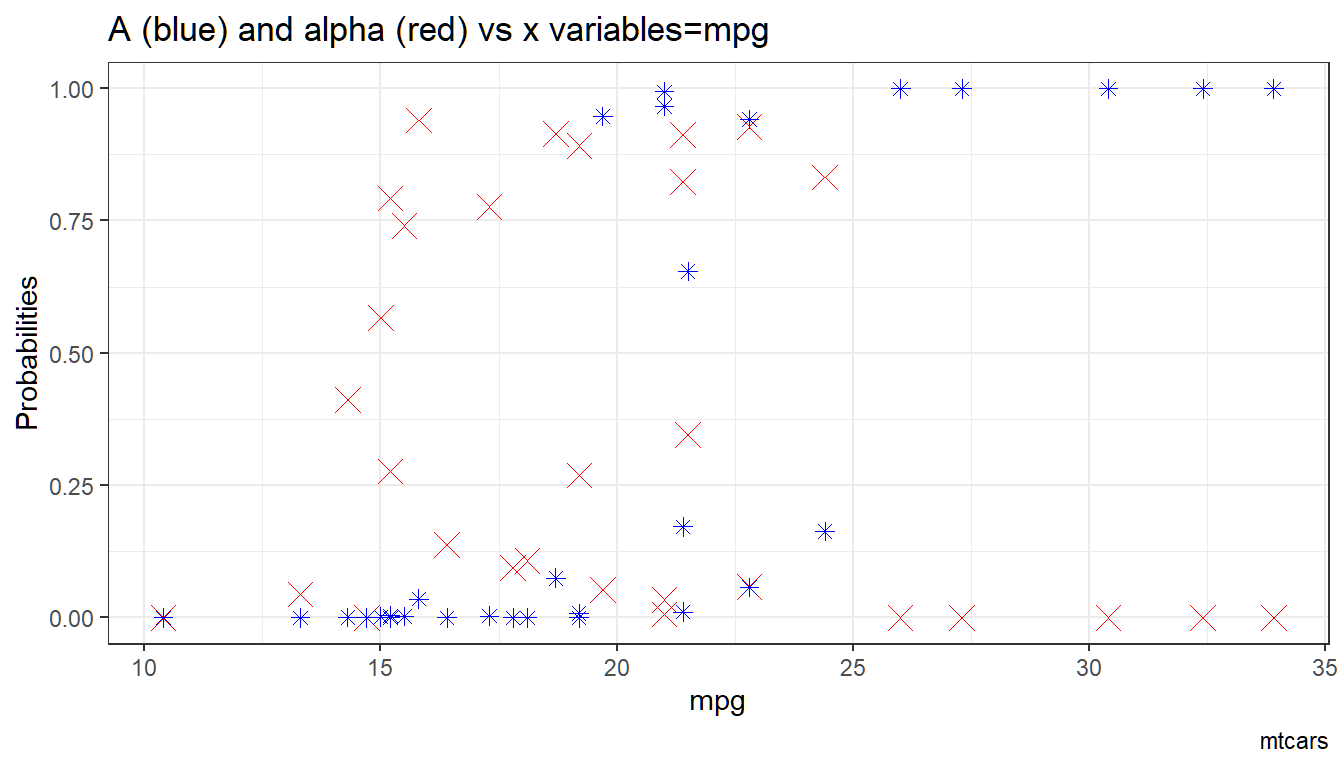
\includegraphics{Panel-Data-and-Optimization-with-R_files/figure-latex/unnamed-chunk-151-1} \end{center}

\hypertarget{linear-regression}{%
\chapter{Linear Regression}\label{linear-regression}}

\hypertarget{ols-and-iv}{%
\section{OLS and IV}\label{ols-and-iv}}

Back to \textbf{\href{https://fanwangecon.github.io/}{Fan}}'s R4Econ Homepage \textbf{\href{https://fanwangecon.github.io/R4Econ/}{Table of Content}}

\hypertarget{ols-and-iv-regression}{%
\subsection{OLS and IV Regression}\label{ols-and-iv-regression}}

\begin{quote}
Go back to \href{http://fanwangecon.github.io/}{fan}'s \href{https://fanwangecon.github.io/REconTools/}{REconTools} Package, \href{https://fanwangecon.github.io/R4Econ/}{R Code Examples} Repository (\href{https://fanwangecon.github.io/R4Econ/bookdown}{bookdown site}), or \href{https://fanwangecon.github.io/Stat4Econ/}{Intro Stats with R} Repository (\href{https://fanwangecon.github.io/Stat4Econ/bookdown}{bookdown site}).
\end{quote}

IV regression using AER package. Option to store all results in dataframe row for combining results from other estimations together. Produce Row Statistics.

\hypertarget{construct-program}{%
\subsubsection{Construct Program}\label{construct-program}}

\begin{Shaded}
\begin{Highlighting}[]
\CommentTok{\# IV regression function}
\CommentTok{\# The code below uses the AER library\textquotesingle{}s regresison function}
\CommentTok{\# All results are stored in a single row as data\_frame}
\CommentTok{\# This functoin could work with dplyr do}
\CommentTok{\# var.y is single outcome, vars.x, vars.c and vars.z are vectors of endogenous variables, controls and instruments.}
\NormalTok{regf.iv }\OtherTok{\textless{}{-}} \ControlFlowTok{function}\NormalTok{(var.y, vars.x, }
\NormalTok{                    vars.c, vars.z, df, }\AttributeTok{transpose=}\ConstantTok{TRUE}\NormalTok{) \{}
  
  \CommentTok{\# A. Set{-}Up Equation}
\NormalTok{  str.vars.x }\OtherTok{\textless{}{-}} \FunctionTok{paste}\NormalTok{(vars.x, }\AttributeTok{collapse=}\StringTok{\textquotesingle{}+\textquotesingle{}}\NormalTok{)}
\NormalTok{  str.vars.c }\OtherTok{\textless{}{-}} \FunctionTok{paste}\NormalTok{(vars.c, }\AttributeTok{collapse=}\StringTok{\textquotesingle{}+\textquotesingle{}}\NormalTok{)}
  
\NormalTok{  df }\OtherTok{\textless{}{-}}\NormalTok{ df }\SpecialCharTok{\%\textgreater{}\%} 
    \FunctionTok{select}\NormalTok{(}\FunctionTok{one\_of}\NormalTok{(var.y, vars.x, vars.c, vars.z)) }\SpecialCharTok{\%\textgreater{}\%} 
    \FunctionTok{drop\_na}\NormalTok{() }\SpecialCharTok{\%\textgreater{}\%} \FunctionTok{filter\_all}\NormalTok{(}\FunctionTok{all\_vars}\NormalTok{(}\SpecialCharTok{!}\FunctionTok{is.infinite}\NormalTok{(.)))}
  
  \ControlFlowTok{if}\NormalTok{ (}\FunctionTok{length}\NormalTok{(vars.z) }\SpecialCharTok{\textgreater{}=} \DecValTok{1}\NormalTok{) \{}
    \CommentTok{\#     library(AER)}
\NormalTok{    str.vars.z }\OtherTok{\textless{}{-}} \FunctionTok{paste}\NormalTok{(vars.z, }\AttributeTok{collapse=}\StringTok{\textquotesingle{}+\textquotesingle{}}\NormalTok{)}
\NormalTok{    equa.iv }\OtherTok{\textless{}{-}} \FunctionTok{paste}\NormalTok{(var.y,}
                     \FunctionTok{paste}\NormalTok{(}\FunctionTok{paste}\NormalTok{(str.vars.x, str.vars.c, }\AttributeTok{sep=}\StringTok{\textquotesingle{}+\textquotesingle{}}\NormalTok{),}
                           \FunctionTok{paste}\NormalTok{(str.vars.z, str.vars.c, }\AttributeTok{sep=}\StringTok{\textquotesingle{}+\textquotesingle{}}\NormalTok{),}
                           \AttributeTok{sep=}\StringTok{\textquotesingle{}|\textquotesingle{}}\NormalTok{),}
                     \AttributeTok{sep=}\StringTok{\textquotesingle{}\textasciitilde{}\textquotesingle{}}\NormalTok{)}
    \CommentTok{\#     print(equa.iv)}
    
    \CommentTok{\# B. IV Regression}
\NormalTok{    ivreg.summ }\OtherTok{\textless{}{-}} \FunctionTok{summary}\NormalTok{(}\FunctionTok{ivreg}\NormalTok{(}\FunctionTok{as.formula}\NormalTok{(equa.iv), }\AttributeTok{data=}\NormalTok{df),}
                          \AttributeTok{vcov =}\NormalTok{ sandwich, }\AttributeTok{df =} \ConstantTok{Inf}\NormalTok{, }\AttributeTok{diagnostics =} \ConstantTok{TRUE}\NormalTok{)}
    
    \CommentTok{\# C. Statistics from IV Regression}
    \CommentTok{\#     ivreg.summ$coef}
    \CommentTok{\#     ivreg.summ$diagnostics}
    
    \CommentTok{\# D. Combine Regression Results into a Matrix}
\NormalTok{    df.results }\OtherTok{\textless{}{-}} \FunctionTok{suppressWarnings}\NormalTok{(}\FunctionTok{suppressMessages}\NormalTok{(}
      \FunctionTok{as\_tibble}\NormalTok{(ivreg.summ}\SpecialCharTok{$}\NormalTok{coef, }\AttributeTok{rownames=}\StringTok{\textquotesingle{}rownames\textquotesingle{}}\NormalTok{) }\SpecialCharTok{\%\textgreater{}\%}
        \FunctionTok{full\_join}\NormalTok{(}\FunctionTok{as\_tibble}\NormalTok{(ivreg.summ}\SpecialCharTok{$}\NormalTok{diagnostics, }\AttributeTok{rownames=}\StringTok{\textquotesingle{}rownames\textquotesingle{}}\NormalTok{)) }\SpecialCharTok{\%\textgreater{}\%}
        \FunctionTok{full\_join}\NormalTok{(}\FunctionTok{tibble}\NormalTok{(}\AttributeTok{rownames=}\FunctionTok{c}\NormalTok{(}\StringTok{\textquotesingle{}vars\textquotesingle{}}\NormalTok{),}
                         \AttributeTok{var.y=}\NormalTok{var.y,}
                         \AttributeTok{vars.x=}\NormalTok{str.vars.x,}
                         \AttributeTok{vars.z=}\NormalTok{str.vars.z,}
                         \AttributeTok{vars.c=}\NormalTok{str.vars.c))))}
\NormalTok{  \} }\ControlFlowTok{else}\NormalTok{ \{}
    
    \CommentTok{\# OLS regression}
\NormalTok{    equa.ols }\OtherTok{\textless{}{-}} \FunctionTok{paste}\NormalTok{(var.y,}
                      \FunctionTok{paste}\NormalTok{(}\FunctionTok{paste}\NormalTok{(vars.x, }\AttributeTok{collapse=}\StringTok{\textquotesingle{}+\textquotesingle{}}\NormalTok{),}
                            \FunctionTok{paste}\NormalTok{(vars.c, }\AttributeTok{collapse=}\StringTok{\textquotesingle{}+\textquotesingle{}}\NormalTok{), }\AttributeTok{sep=}\StringTok{\textquotesingle{}+\textquotesingle{}}\NormalTok{),}
                      \AttributeTok{sep=}\StringTok{\textquotesingle{}\textasciitilde{}\textquotesingle{}}\NormalTok{)}
    
\NormalTok{    lmreg.summ }\OtherTok{\textless{}{-}} \FunctionTok{summary}\NormalTok{(}\FunctionTok{lm}\NormalTok{(}\FunctionTok{as.formula}\NormalTok{(equa.ols), }\AttributeTok{data=}\NormalTok{df))}
    
\NormalTok{    lm.diagnostics }\OtherTok{\textless{}{-}} \FunctionTok{as\_tibble}\NormalTok{(}
      \FunctionTok{list}\NormalTok{(}\AttributeTok{df1=}\NormalTok{lmreg.summ}\SpecialCharTok{$}\NormalTok{df[[}\DecValTok{1}\NormalTok{]],}
           \AttributeTok{df2=}\NormalTok{lmreg.summ}\SpecialCharTok{$}\NormalTok{df[[}\DecValTok{2}\NormalTok{]],}
           \AttributeTok{df3=}\NormalTok{lmreg.summ}\SpecialCharTok{$}\NormalTok{df[[}\DecValTok{3}\NormalTok{]],}
           \AttributeTok{sigma=}\NormalTok{lmreg.summ}\SpecialCharTok{$}\NormalTok{sigma,}
           \AttributeTok{r.squared=}\NormalTok{lmreg.summ}\SpecialCharTok{$}\NormalTok{r.squared,}
           \AttributeTok{adj.r.squared=}\NormalTok{lmreg.summ}\SpecialCharTok{$}\NormalTok{adj.r.squared)) }\SpecialCharTok{\%\textgreater{}\%}
      \FunctionTok{gather}\NormalTok{(variable, value) }\SpecialCharTok{\%\textgreater{}\%}
      \FunctionTok{rename}\NormalTok{(}\AttributeTok{rownames =}\NormalTok{ variable) }\SpecialCharTok{\%\textgreater{}\%}
      \FunctionTok{rename}\NormalTok{(}\AttributeTok{v =}\NormalTok{ value)}
    
\NormalTok{    df.results }\OtherTok{\textless{}{-}} \FunctionTok{suppressWarnings}\NormalTok{(}\FunctionTok{suppressMessages}\NormalTok{(}
      \FunctionTok{as\_tibble}\NormalTok{(lmreg.summ}\SpecialCharTok{$}\NormalTok{coef, }\AttributeTok{rownames=}\StringTok{\textquotesingle{}rownames\textquotesingle{}}\NormalTok{) }\SpecialCharTok{\%\textgreater{}\%}
        \FunctionTok{full\_join}\NormalTok{(lm.diagnostics) }\SpecialCharTok{\%\textgreater{}\%}
        \FunctionTok{full\_join}\NormalTok{(}\FunctionTok{tibble}\NormalTok{(}\AttributeTok{rownames=}\FunctionTok{c}\NormalTok{(}\StringTok{\textquotesingle{}vars\textquotesingle{}}\NormalTok{),}
                         \AttributeTok{var.y=}\NormalTok{var.y,}
                         \AttributeTok{vars.x=}\NormalTok{str.vars.x,}
                         \AttributeTok{vars.c=}\NormalTok{str.vars.c))))}
\NormalTok{  \}}
  
  \CommentTok{\# E. Flatten Matrix, All IV results as a single tibble }
  \CommentTok{\# row to be combined with other IV results}
\NormalTok{  df.row.results }\OtherTok{\textless{}{-}}\NormalTok{ df.results }\SpecialCharTok{\%\textgreater{}\%}
    \FunctionTok{gather}\NormalTok{(variable, value, }\SpecialCharTok{{-}}\NormalTok{rownames) }\SpecialCharTok{\%\textgreater{}\%}
    \FunctionTok{drop\_na}\NormalTok{() }\SpecialCharTok{\%\textgreater{}\%}
    \FunctionTok{unite}\NormalTok{(esti.val, rownames, variable) }\SpecialCharTok{\%\textgreater{}\%}
    \FunctionTok{mutate}\NormalTok{(}\AttributeTok{esti.val =} \FunctionTok{gsub}\NormalTok{(}\StringTok{\textquotesingle{} \textquotesingle{}}\NormalTok{, }\StringTok{\textquotesingle{}\textquotesingle{}}\NormalTok{, esti.val))}
  
  \ControlFlowTok{if}\NormalTok{ (transpose) \{}
\NormalTok{    df.row.results }\OtherTok{\textless{}{-}}\NormalTok{ df.row.results }\SpecialCharTok{\%\textgreater{}\%} \FunctionTok{spread}\NormalTok{(esti.val, value)}
\NormalTok{  \}}
  
  \CommentTok{\# F. Return}
  \FunctionTok{return}\NormalTok{(}\FunctionTok{data.frame}\NormalTok{(df.row.results))}
\NormalTok{\}}
\end{Highlighting}
\end{Shaded}

\hypertarget{program-testing}{%
\subsubsection{Program Testing}\label{program-testing}}

Load Data

\begin{Shaded}
\begin{Highlighting}[]
\CommentTok{\# Library}
\FunctionTok{library}\NormalTok{(tidyverse)}
\FunctionTok{library}\NormalTok{(AER)}

\CommentTok{\# Load Sample Data}
\FunctionTok{setwd}\NormalTok{(}\StringTok{\textquotesingle{}C:/Users/fan/R4Econ/\_data/\textquotesingle{}}\NormalTok{)}
\NormalTok{df }\OtherTok{\textless{}{-}} \FunctionTok{read\_csv}\NormalTok{(}\StringTok{\textquotesingle{}height\_weight.csv\textquotesingle{}}\NormalTok{)}
\end{Highlighting}
\end{Shaded}

\hypertarget{example-no-instrument-ols}{%
\paragraph{Example No Instrument, OLS}\label{example-no-instrument-ols}}

\begin{Shaded}
\begin{Highlighting}[]
\CommentTok{\# One Instrucments}
\NormalTok{var.y }\OtherTok{\textless{}{-}} \FunctionTok{c}\NormalTok{(}\StringTok{\textquotesingle{}hgt\textquotesingle{}}\NormalTok{)}
\NormalTok{vars.x }\OtherTok{\textless{}{-}} \FunctionTok{c}\NormalTok{(}\StringTok{\textquotesingle{}prot\textquotesingle{}}\NormalTok{)}
\NormalTok{vars.z }\OtherTok{\textless{}{-}} \ConstantTok{NULL}
\NormalTok{vars.c }\OtherTok{\textless{}{-}} \FunctionTok{c}\NormalTok{(}\StringTok{\textquotesingle{}sex\textquotesingle{}}\NormalTok{, }\StringTok{\textquotesingle{}hgt0\textquotesingle{}}\NormalTok{, }\StringTok{\textquotesingle{}wgt0\textquotesingle{}}\NormalTok{)}
\CommentTok{\# Regression}
\FunctionTok{regf.iv}\NormalTok{(var.y, vars.x, vars.c, vars.z, df, }\AttributeTok{transpose=}\ConstantTok{FALSE}\NormalTok{) }\SpecialCharTok{\%\textgreater{}\%}
  \FunctionTok{kable}\NormalTok{() }\SpecialCharTok{\%\textgreater{}\%}
  \FunctionTok{kable\_styling\_fc}\NormalTok{()}
\end{Highlighting}
\end{Shaded}

\begin{table}[!h]
\centering
\begin{tabular}{l|l}
\hline
esti.val & value\\
\hline
\cellcolor{gray!6}{(Intercept)\_Estimate} & \cellcolor{gray!6}{52.1186286658651}\\
\hline
prot\_Estimate & 0.374472386357917\\
\hline
\cellcolor{gray!6}{sexMale\_Estimate} & \cellcolor{gray!6}{0.611043720578292}\\
\hline
hgt0\_Estimate & 0.148513781160842\\
\hline
\cellcolor{gray!6}{wgt0\_Estimate} & \cellcolor{gray!6}{0.00150560230505631}\\
\hline
(Intercept)\_Std.Error & 1.57770483608693\\
\hline
\cellcolor{gray!6}{prot\_Std.Error} & \cellcolor{gray!6}{0.00418121191133815}\\
\hline
sexMale\_Std.Error & 0.118396259120659\\
\hline
\cellcolor{gray!6}{hgt0\_Std.Error} & \cellcolor{gray!6}{0.0393807494783186}\\
\hline
wgt0\_Std.Error & 0.000187123663624397\\
\hline
\cellcolor{gray!6}{(Intercept)\_tvalue} & \cellcolor{gray!6}{33.0344608660332}\\
\hline
prot\_tvalue & 89.5607288744356\\
\hline
\cellcolor{gray!6}{sexMale\_tvalue} & \cellcolor{gray!6}{5.16100529794248}\\
\hline
hgt0\_tvalue & 3.77122790013449\\
\hline
\cellcolor{gray!6}{wgt0\_tvalue} & \cellcolor{gray!6}{8.04602836377991}\\
\hline
(Intercept)\_Pr(>|t|) & 9.92126150975783e-233\\
\hline
\cellcolor{gray!6}{prot\_Pr(>|t|)} & \cellcolor{gray!6}{0}\\
\hline
sexMale\_Pr(>|t|) & 2.48105505495642e-07\\
\hline
\cellcolor{gray!6}{hgt0\_Pr(>|t|)} & \cellcolor{gray!6}{0.000162939618371183}\\
\hline
wgt0\_Pr(>|t|) & 9.05257561534111e-16\\
\hline
\cellcolor{gray!6}{df1\_v} & \cellcolor{gray!6}{5}\\
\hline
df2\_v & 18958\\
\hline
\cellcolor{gray!6}{df3\_v} & \cellcolor{gray!6}{5}\\
\hline
sigma\_v & 8.06197784622979\\
\hline
\cellcolor{gray!6}{r.squared\_v} & \cellcolor{gray!6}{0.319078711001325}\\
\hline
adj.r.squared\_v & 0.318935041565942\\
\hline
\cellcolor{gray!6}{vars\_var.y} & \cellcolor{gray!6}{hgt}\\
\hline
vars\_vars.x & prot\\
\hline
\cellcolor{gray!6}{vars\_vars.c} & \cellcolor{gray!6}{sex+hgt0+wgt0}\\
\hline
\end{tabular}
\end{table}

\hypertarget{example-1-insturment}{%
\paragraph{Example 1 Insturment}\label{example-1-insturment}}

\begin{Shaded}
\begin{Highlighting}[]
\CommentTok{\# One Instrucments}
\NormalTok{var.y }\OtherTok{\textless{}{-}} \FunctionTok{c}\NormalTok{(}\StringTok{\textquotesingle{}hgt\textquotesingle{}}\NormalTok{)}
\NormalTok{vars.x }\OtherTok{\textless{}{-}} \FunctionTok{c}\NormalTok{(}\StringTok{\textquotesingle{}prot\textquotesingle{}}\NormalTok{)}
\NormalTok{vars.z }\OtherTok{\textless{}{-}} \FunctionTok{c}\NormalTok{(}\StringTok{\textquotesingle{}momEdu\textquotesingle{}}\NormalTok{)}
\NormalTok{vars.c }\OtherTok{\textless{}{-}} \FunctionTok{c}\NormalTok{(}\StringTok{\textquotesingle{}sex\textquotesingle{}}\NormalTok{, }\StringTok{\textquotesingle{}hgt0\textquotesingle{}}\NormalTok{, }\StringTok{\textquotesingle{}wgt0\textquotesingle{}}\NormalTok{)}
\CommentTok{\# Regression}
\FunctionTok{regf.iv}\NormalTok{(var.y, vars.x, vars.c, vars.z, df, }\AttributeTok{transpose=}\ConstantTok{FALSE}\NormalTok{) }\SpecialCharTok{\%\textgreater{}\%}
  \FunctionTok{kable}\NormalTok{() }\SpecialCharTok{\%\textgreater{}\%}
  \FunctionTok{kable\_styling\_fc}\NormalTok{()}
\end{Highlighting}
\end{Shaded}

\begin{table}[!h]
\centering
\begin{tabular}{l|l}
\hline
esti.val & value\\
\hline
\cellcolor{gray!6}{(Intercept)\_Estimate} & \cellcolor{gray!6}{43.4301969117558}\\
\hline
prot\_Estimate & 0.130833343849446\\
\hline
\cellcolor{gray!6}{sexMale\_Estimate} & \cellcolor{gray!6}{0.868121847262411}\\
\hline
hgt0\_Estimate & 0.412093881817148\\
\hline
\cellcolor{gray!6}{wgt0\_Estimate} & \cellcolor{gray!6}{0.000858630042617921}\\
\hline
(Intercept)\_Std.Error & 1.82489550971182\\
\hline
\cellcolor{gray!6}{prot\_Std.Error} & \cellcolor{gray!6}{0.0192036220809189}\\
\hline
sexMale\_Std.Error & 0.13373016700542\\
\hline
\cellcolor{gray!6}{hgt0\_Std.Error} & \cellcolor{gray!6}{0.0459431912927002}\\
\hline
wgt0\_Std.Error & 0.00022691057702563\\
\hline
\cellcolor{gray!6}{(Intercept)\_zvalue} & \cellcolor{gray!6}{23.798730766023}\\
\hline
prot\_zvalue & 6.81295139521853\\
\hline
\cellcolor{gray!6}{sexMale\_zvalue} & \cellcolor{gray!6}{6.49159323361366}\\
\hline
hgt0\_zvalue & 8.96963990141069\\
\hline
\cellcolor{gray!6}{wgt0\_zvalue} & \cellcolor{gray!6}{3.7840018472164}\\
\hline
(Intercept)\_Pr(>|z|) & 3.4423766196876e-125\\
\hline
\cellcolor{gray!6}{prot\_Pr(>|z|)} & \cellcolor{gray!6}{9.56164541643828e-12}\\
\hline
sexMale\_Pr(>|z|) & 8.49333228172763e-11\\
\hline
\cellcolor{gray!6}{hgt0\_Pr(>|z|)} & \cellcolor{gray!6}{2.97485394526792e-19}\\
\hline
wgt0\_Pr(>|z|) & 0.000154326676608523\\
\hline
\cellcolor{gray!6}{Weakinstruments\_df1} & \cellcolor{gray!6}{1}\\
\hline
Wu-Hausman\_df1 & 1\\
\hline
\cellcolor{gray!6}{Sargan\_df1} & \cellcolor{gray!6}{0}\\
\hline
Weakinstruments\_df2 & 16394\\
\hline
\cellcolor{gray!6}{Wu-Hausman\_df2} & \cellcolor{gray!6}{16393}\\
\hline
Weakinstruments\_statistic & 935.817456612075\\
\hline
\cellcolor{gray!6}{Wu-Hausman\_statistic} & \cellcolor{gray!6}{123.595856606729}\\
\hline
Weakinstruments\_p-value & 6.39714929178024e-200\\
\hline
\cellcolor{gray!6}{Wu-Hausman\_p-value} & \cellcolor{gray!6}{1.30703637796748e-28}\\
\hline
vars\_var.y & hgt\\
\hline
\cellcolor{gray!6}{vars\_vars.x} & \cellcolor{gray!6}{prot}\\
\hline
vars\_vars.z & momEdu\\
\hline
\cellcolor{gray!6}{vars\_vars.c} & \cellcolor{gray!6}{sex+hgt0+wgt0}\\
\hline
\end{tabular}
\end{table}

\hypertarget{example-multiple-instrucments}{%
\paragraph{Example Multiple Instrucments}\label{example-multiple-instrucments}}

\begin{Shaded}
\begin{Highlighting}[]
\CommentTok{\# Multiple Instrucments}
\NormalTok{var.y }\OtherTok{\textless{}{-}} \FunctionTok{c}\NormalTok{(}\StringTok{\textquotesingle{}hgt\textquotesingle{}}\NormalTok{)}
\NormalTok{vars.x }\OtherTok{\textless{}{-}} \FunctionTok{c}\NormalTok{(}\StringTok{\textquotesingle{}prot\textquotesingle{}}\NormalTok{)}
\NormalTok{vars.z }\OtherTok{\textless{}{-}} \FunctionTok{c}\NormalTok{(}\StringTok{\textquotesingle{}momEdu\textquotesingle{}}\NormalTok{, }\StringTok{\textquotesingle{}wealthIdx\textquotesingle{}}\NormalTok{, }\StringTok{\textquotesingle{}p.A.prot\textquotesingle{}}\NormalTok{, }\StringTok{\textquotesingle{}p.A.nProt\textquotesingle{}}\NormalTok{)}
\NormalTok{vars.c }\OtherTok{\textless{}{-}} \FunctionTok{c}\NormalTok{(}\StringTok{\textquotesingle{}sex\textquotesingle{}}\NormalTok{, }\StringTok{\textquotesingle{}hgt0\textquotesingle{}}\NormalTok{, }\StringTok{\textquotesingle{}wgt0\textquotesingle{}}\NormalTok{)}
\CommentTok{\# Regression}
\FunctionTok{regf.iv}\NormalTok{(var.y, vars.x, vars.c, vars.z, df, }\AttributeTok{transpose=}\ConstantTok{FALSE}\NormalTok{) }\SpecialCharTok{\%\textgreater{}\%}
  \FunctionTok{kable}\NormalTok{() }\SpecialCharTok{\%\textgreater{}\%}
  \FunctionTok{kable\_styling\_fc}\NormalTok{()}
\end{Highlighting}
\end{Shaded}

\begin{table}[!h]
\centering
\begin{tabular}{l|l}
\hline
esti.val & value\\
\hline
\cellcolor{gray!6}{(Intercept)\_Estimate} & \cellcolor{gray!6}{42.2437613555242}\\
\hline
prot\_Estimate & 0.26699945194704\\
\hline
\cellcolor{gray!6}{sexMale\_Estimate} & \cellcolor{gray!6}{0.695548488812932}\\
\hline
hgt0\_Estimate & 0.424954881263031\\
\hline
\cellcolor{gray!6}{wgt0\_Estimate} & \cellcolor{gray!6}{0.000486951420329484}\\
\hline
(Intercept)\_Std.Error & 1.85356686789642\\
\hline
\cellcolor{gray!6}{prot\_Std.Error} & \cellcolor{gray!6}{0.0154939347964083}\\
\hline
sexMale\_Std.Error & 0.133157977814374\\
\hline
\cellcolor{gray!6}{hgt0\_Std.Error} & \cellcolor{gray!6}{0.0463195803786233}\\
\hline
wgt0\_Std.Error & 0.000224867994873235\\
\hline
\cellcolor{gray!6}{(Intercept)\_zvalue} & \cellcolor{gray!6}{22.7905246296649}\\
\hline
prot\_zvalue & 17.2325142357597\\
\hline
\cellcolor{gray!6}{sexMale\_zvalue} & \cellcolor{gray!6}{5.22348341593581}\\
\hline
hgt0\_zvalue & 9.17441129192849\\
\hline
\cellcolor{gray!6}{wgt0\_zvalue} & \cellcolor{gray!6}{2.16549901022595}\\
\hline
(Intercept)\_Pr(>|z|) & 5.69294074735747e-115\\
\hline
\cellcolor{gray!6}{prot\_Pr(>|z|)} & \cellcolor{gray!6}{1.51424021931607e-66}\\
\hline
sexMale\_Pr(>|z|) & 1.75588197502565e-07\\
\hline
\cellcolor{gray!6}{hgt0\_Pr(>|z|)} & \cellcolor{gray!6}{4.54048595587756e-20}\\
\hline
wgt0\_Pr(>|z|) & 0.030349491114332\\
\hline
\cellcolor{gray!6}{Weakinstruments\_df1} & \cellcolor{gray!6}{4}\\
\hline
Wu-Hausman\_df1 & 1\\
\hline
\cellcolor{gray!6}{Sargan\_df1} & \cellcolor{gray!6}{3}\\
\hline
Weakinstruments\_df2 & 14914\\
\hline
\cellcolor{gray!6}{Wu-Hausman\_df2} & \cellcolor{gray!6}{14916}\\
\hline
Weakinstruments\_statistic & 274.147084958343\\
\hline
\cellcolor{gray!6}{Wu-Hausman\_statistic} & \cellcolor{gray!6}{17.7562545747101}\\
\hline
Sargan\_statistic & 463.729664547249\\
\hline
\cellcolor{gray!6}{Weakinstruments\_p-value} & \cellcolor{gray!6}{8.61731956233366e-228}\\
\hline
Wu-Hausman\_p-value & 2.52567249124181e-05\\
\hline
\cellcolor{gray!6}{Sargan\_p-value} & \cellcolor{gray!6}{3.45452874915475e-100}\\
\hline
vars\_var.y & hgt\\
\hline
\cellcolor{gray!6}{vars\_vars.x} & \cellcolor{gray!6}{prot}\\
\hline
vars\_vars.z & momEdu+wealthIdx+p.A.prot+p.A.nProt\\
\hline
\cellcolor{gray!6}{vars\_vars.c} & \cellcolor{gray!6}{sex+hgt0+wgt0}\\
\hline
\end{tabular}
\end{table}

\hypertarget{example-multiple-endogenous-variables}{%
\paragraph{Example Multiple Endogenous Variables}\label{example-multiple-endogenous-variables}}

\begin{Shaded}
\begin{Highlighting}[]
\CommentTok{\# Multiple Instrucments}
\NormalTok{var.y }\OtherTok{\textless{}{-}} \FunctionTok{c}\NormalTok{(}\StringTok{\textquotesingle{}hgt\textquotesingle{}}\NormalTok{)}
\NormalTok{vars.x }\OtherTok{\textless{}{-}} \FunctionTok{c}\NormalTok{(}\StringTok{\textquotesingle{}prot\textquotesingle{}}\NormalTok{, }\StringTok{\textquotesingle{}cal\textquotesingle{}}\NormalTok{)}
\NormalTok{vars.z }\OtherTok{\textless{}{-}} \FunctionTok{c}\NormalTok{(}\StringTok{\textquotesingle{}momEdu\textquotesingle{}}\NormalTok{, }\StringTok{\textquotesingle{}wealthIdx\textquotesingle{}}\NormalTok{, }\StringTok{\textquotesingle{}p.A.prot\textquotesingle{}}\NormalTok{, }\StringTok{\textquotesingle{}p.A.nProt\textquotesingle{}}\NormalTok{)}
\NormalTok{vars.c }\OtherTok{\textless{}{-}} \FunctionTok{c}\NormalTok{(}\StringTok{\textquotesingle{}sex\textquotesingle{}}\NormalTok{, }\StringTok{\textquotesingle{}hgt0\textquotesingle{}}\NormalTok{, }\StringTok{\textquotesingle{}wgt0\textquotesingle{}}\NormalTok{)}
\CommentTok{\# Regression}
\FunctionTok{regf.iv}\NormalTok{(var.y, vars.x, vars.c, vars.z, df, }\AttributeTok{transpose=}\ConstantTok{FALSE}\NormalTok{) }\SpecialCharTok{\%\textgreater{}\%}
  \FunctionTok{kable}\NormalTok{() }\SpecialCharTok{\%\textgreater{}\%}
  \FunctionTok{kable\_styling\_fc}\NormalTok{()}
\end{Highlighting}
\end{Shaded}

\begin{table}[!h]
\centering
\begin{tabular}{l|l}
\hline
esti.val & value\\
\hline
\cellcolor{gray!6}{(Intercept)\_Estimate} & \cellcolor{gray!6}{44.0243196254297}\\
\hline
prot\_Estimate & -1.4025623247106\\
\hline
\cellcolor{gray!6}{cal\_Estimate} & \cellcolor{gray!6}{0.065104895750151}\\
\hline
sexMale\_Estimate & 0.120832787571818\\
\hline
\cellcolor{gray!6}{hgt0\_Estimate} & \cellcolor{gray!6}{0.286525437984517}\\
\hline
wgt0\_Estimate & 0.000850481389651033\\
\hline
\cellcolor{gray!6}{(Intercept)\_Std.Error} & \cellcolor{gray!6}{2.75354847244082}\\
\hline
prot\_Std.Error & 0.198640060273635\\
\hline
\cellcolor{gray!6}{cal\_Std.Error} & \cellcolor{gray!6}{0.00758881298880996}\\
\hline
sexMale\_Std.Error & 0.209984580636303\\
\hline
\cellcolor{gray!6}{hgt0\_Std.Error} & \cellcolor{gray!6}{0.0707828182888255}\\
\hline
wgt0\_Std.Error & 0.00033711210444429\\
\hline
\cellcolor{gray!6}{(Intercept)\_zvalue} & \cellcolor{gray!6}{15.9882130516502}\\
\hline
prot\_zvalue & -7.06082309267581\\
\hline
\cellcolor{gray!6}{cal\_zvalue} & \cellcolor{gray!6}{8.57906181719737}\\
\hline
sexMale\_zvalue & 0.575436478267434\\
\hline
\cellcolor{gray!6}{hgt0\_zvalue} & \cellcolor{gray!6}{4.04795181812859}\\
\hline
wgt0\_zvalue & 2.52284441418383\\
\hline
\cellcolor{gray!6}{(Intercept)\_Pr(>|z|)} & \cellcolor{gray!6}{1.54396598126854e-57}\\
\hline
prot\_Pr(>|z|) & 1.65519210848649e-12\\
\hline
\cellcolor{gray!6}{cal\_Pr(>|z|)} & \cellcolor{gray!6}{9.56500648203187e-18}\\
\hline
sexMale\_Pr(>|z|) & 0.564996139463599\\
\hline
\cellcolor{gray!6}{hgt0\_Pr(>|z|)} & \cellcolor{gray!6}{5.16677787108928e-05}\\
\hline
wgt0\_Pr(>|z|) & 0.0116409892837831\\
\hline
\cellcolor{gray!6}{Weakinstruments(prot)\_df1} & \cellcolor{gray!6}{4}\\
\hline
Weakinstruments(cal)\_df1 & 4\\
\hline
\cellcolor{gray!6}{Wu-Hausman\_df1} & \cellcolor{gray!6}{2}\\
\hline
Sargan\_df1 & 2\\
\hline
\cellcolor{gray!6}{Weakinstruments(prot)\_df2} & \cellcolor{gray!6}{14914}\\
\hline
Weakinstruments(cal)\_df2 & 14914\\
\hline
\cellcolor{gray!6}{Wu-Hausman\_df2} & \cellcolor{gray!6}{14914}\\
\hline
Weakinstruments(prot)\_statistic & 274.147084958343\\
\hline
\cellcolor{gray!6}{Weakinstruments(cal)\_statistic} & \cellcolor{gray!6}{315.036848606231}\\
\hline
Wu-Hausman\_statistic & 94.7020085425169\\
\hline
\cellcolor{gray!6}{Sargan\_statistic} & \cellcolor{gray!6}{122.081979628898}\\
\hline
Weakinstruments(prot)\_p-value & 8.61731956233366e-228\\
\hline
\cellcolor{gray!6}{Weakinstruments(cal)\_p-value} & \cellcolor{gray!6}{1.18918641220866e-260}\\
\hline
Wu-Hausman\_p-value & 1.35024050408262e-41\\
\hline
\cellcolor{gray!6}{Sargan\_p-value} & \cellcolor{gray!6}{3.09196773720398e-27}\\
\hline
vars\_var.y & hgt\\
\hline
\cellcolor{gray!6}{vars\_vars.x} & \cellcolor{gray!6}{prot+cal}\\
\hline
vars\_vars.z & momEdu+wealthIdx+p.A.prot+p.A.nProt\\
\hline
\cellcolor{gray!6}{vars\_vars.c} & \cellcolor{gray!6}{sex+hgt0+wgt0}\\
\hline
\end{tabular}
\end{table}

\hypertarget{examples-line-by-line}{%
\paragraph{Examples Line by Line}\label{examples-line-by-line}}

The examples are just to test the code with different types of variables.

\begin{Shaded}
\begin{Highlighting}[]
\CommentTok{\# Selecting Variables}
\NormalTok{var.y }\OtherTok{\textless{}{-}} \FunctionTok{c}\NormalTok{(}\StringTok{\textquotesingle{}hgt\textquotesingle{}}\NormalTok{)}
\NormalTok{vars.x }\OtherTok{\textless{}{-}} \FunctionTok{c}\NormalTok{(}\StringTok{\textquotesingle{}prot\textquotesingle{}}\NormalTok{, }\StringTok{\textquotesingle{}cal\textquotesingle{}}\NormalTok{)}
\NormalTok{vars.z }\OtherTok{\textless{}{-}} \FunctionTok{c}\NormalTok{(}\StringTok{\textquotesingle{}momEdu\textquotesingle{}}\NormalTok{, }\StringTok{\textquotesingle{}wealthIdx\textquotesingle{}}\NormalTok{, }\StringTok{\textquotesingle{}p.A.prot\textquotesingle{}}\NormalTok{, }\StringTok{\textquotesingle{}p.A.nProt\textquotesingle{}}\NormalTok{)}
\NormalTok{vars.c }\OtherTok{\textless{}{-}} \FunctionTok{c}\NormalTok{(}\StringTok{\textquotesingle{}sex\textquotesingle{}}\NormalTok{, }\StringTok{\textquotesingle{}hgt0\textquotesingle{}}\NormalTok{, }\StringTok{\textquotesingle{}wgt0\textquotesingle{}}\NormalTok{)}
\end{Highlighting}
\end{Shaded}

\begin{Shaded}
\begin{Highlighting}[]
\CommentTok{\# A. create Equation}
\NormalTok{str.vars.x }\OtherTok{\textless{}{-}} \FunctionTok{paste}\NormalTok{(vars.x, }\AttributeTok{collapse=}\StringTok{\textquotesingle{}+\textquotesingle{}}\NormalTok{)}
\NormalTok{str.vars.c }\OtherTok{\textless{}{-}} \FunctionTok{paste}\NormalTok{(vars.c, }\AttributeTok{collapse=}\StringTok{\textquotesingle{}+\textquotesingle{}}\NormalTok{)}
\NormalTok{str.vars.z }\OtherTok{\textless{}{-}} \FunctionTok{paste}\NormalTok{(vars.z, }\AttributeTok{collapse=}\StringTok{\textquotesingle{}+\textquotesingle{}}\NormalTok{)}
\FunctionTok{print}\NormalTok{(str.vars.x)}
\end{Highlighting}
\end{Shaded}

\begin{verbatim}
## [1] "prot+cal"
\end{verbatim}

\begin{Shaded}
\begin{Highlighting}[]
\FunctionTok{print}\NormalTok{(str.vars.c)}
\end{Highlighting}
\end{Shaded}

\begin{verbatim}
## [1] "sex+hgt0+wgt0"
\end{verbatim}

\begin{Shaded}
\begin{Highlighting}[]
\FunctionTok{print}\NormalTok{(str.vars.z)}
\end{Highlighting}
\end{Shaded}

\begin{verbatim}
## [1] "momEdu+wealthIdx+p.A.prot+p.A.nProt"
\end{verbatim}

\begin{Shaded}
\begin{Highlighting}[]
\NormalTok{equa.iv }\OtherTok{\textless{}{-}} \FunctionTok{paste}\NormalTok{(var.y,}
                 \FunctionTok{paste}\NormalTok{(}\FunctionTok{paste}\NormalTok{(str.vars.x, str.vars.c, }\AttributeTok{sep=}\StringTok{\textquotesingle{}+\textquotesingle{}}\NormalTok{),}
                       \FunctionTok{paste}\NormalTok{(str.vars.z, str.vars.c, }\AttributeTok{sep=}\StringTok{\textquotesingle{}+\textquotesingle{}}\NormalTok{),}
                       \AttributeTok{sep=}\StringTok{\textquotesingle{}|\textquotesingle{}}\NormalTok{),}
                 \AttributeTok{sep=}\StringTok{\textquotesingle{}\textasciitilde{}\textquotesingle{}}\NormalTok{)}
\FunctionTok{print}\NormalTok{(equa.iv)}
\end{Highlighting}
\end{Shaded}

\begin{verbatim}
## [1] "hgt~prot+cal+sex+hgt0+wgt0|momEdu+wealthIdx+p.A.prot+p.A.nProt+sex+hgt0+wgt0"
\end{verbatim}

\begin{Shaded}
\begin{Highlighting}[]
\CommentTok{\# B. regression}
\NormalTok{res.ivreg }\OtherTok{\textless{}{-}} \FunctionTok{ivreg}\NormalTok{(}\FunctionTok{as.formula}\NormalTok{(equa.iv), }\AttributeTok{data=}\NormalTok{df)}
\FunctionTok{coef}\NormalTok{(res.ivreg)}
\end{Highlighting}
\end{Shaded}

\begin{verbatim}
##   (Intercept)          prot           cal       sexMale          hgt0          wgt0 
## 44.0243196254 -1.4025623247  0.0651048958  0.1208327876  0.2865254380  0.0008504814
\end{verbatim}

\begin{Shaded}
\begin{Highlighting}[]
\CommentTok{\# C. Regression Summary}
\NormalTok{ivreg.summ }\OtherTok{\textless{}{-}} \FunctionTok{summary}\NormalTok{(res.ivreg, }\AttributeTok{vcov =}\NormalTok{ sandwich, }\AttributeTok{df =} \ConstantTok{Inf}\NormalTok{, }\AttributeTok{diagnostics =} \ConstantTok{TRUE}\NormalTok{)}

\NormalTok{ivreg.summ}\SpecialCharTok{$}\NormalTok{coef}
\end{Highlighting}
\end{Shaded}

\begin{verbatim}
##                  Estimate   Std. Error    z value     Pr(>|z|)
## (Intercept) 44.0243196254 2.7535484724 15.9882131 1.543966e-57
## prot        -1.4025623247 0.1986400603 -7.0608231 1.655192e-12
## cal          0.0651048958 0.0075888130  8.5790618 9.565006e-18
## sexMale      0.1208327876 0.2099845806  0.5754365 5.649961e-01
## hgt0         0.2865254380 0.0707828183  4.0479518 5.166778e-05
## wgt0         0.0008504814 0.0003371121  2.5228444 1.164099e-02
## attr(,"df")
## [1] 0
## attr(,"nobs")
## [1] 14922
\end{verbatim}

\begin{Shaded}
\begin{Highlighting}[]
\NormalTok{ivreg.summ}\SpecialCharTok{$}\NormalTok{diagnostics}
\end{Highlighting}
\end{Shaded}

\begin{verbatim}
##                         df1   df2 statistic       p-value
## Weak instruments (prot)   4 14914 274.14708 8.617320e-228
## Weak instruments (cal)    4 14914 315.03685 1.189186e-260
## Wu-Hausman                2 14914  94.70201  1.350241e-41
## Sargan                    2    NA 122.08198  3.091968e-27
\end{verbatim}

\begin{Shaded}
\begin{Highlighting}[]
\CommentTok{\# D. Combine Regression Results into a Matrix}
\NormalTok{df.results }\OtherTok{\textless{}{-}} \FunctionTok{suppressMessages}\NormalTok{(}\FunctionTok{as\_tibble}\NormalTok{(ivreg.summ}\SpecialCharTok{$}\NormalTok{coef, }\AttributeTok{rownames=}\StringTok{\textquotesingle{}rownames\textquotesingle{}}\NormalTok{) }\SpecialCharTok{\%\textgreater{}\%}
    \FunctionTok{full\_join}\NormalTok{(}\FunctionTok{as\_tibble}\NormalTok{(ivreg.summ}\SpecialCharTok{$}\NormalTok{diagnostics, }\AttributeTok{rownames=}\StringTok{\textquotesingle{}rownames\textquotesingle{}}\NormalTok{)) }\SpecialCharTok{\%\textgreater{}\%}
    \FunctionTok{full\_join}\NormalTok{(}\FunctionTok{tibble}\NormalTok{(}\AttributeTok{rownames=}\FunctionTok{c}\NormalTok{(}\StringTok{\textquotesingle{}vars\textquotesingle{}}\NormalTok{),}
                     \AttributeTok{var.y=}\NormalTok{var.y,}
                     \AttributeTok{vars.x=}\NormalTok{str.vars.x,}
                     \AttributeTok{vars.z=}\NormalTok{str.vars.z,}
                     \AttributeTok{vars.c=}\NormalTok{str.vars.c)))}
\CommentTok{\# E. Flatten Matrix, All IV results as a single tibble row to be combined with other IV results}
\NormalTok{df.row.results }\OtherTok{\textless{}{-}}\NormalTok{ df.results }\SpecialCharTok{\%\textgreater{}\%}
    \FunctionTok{gather}\NormalTok{(variable, value, }\SpecialCharTok{{-}}\NormalTok{rownames) }\SpecialCharTok{\%\textgreater{}\%}
    \FunctionTok{drop\_na}\NormalTok{() }\SpecialCharTok{\%\textgreater{}\%}
    \FunctionTok{unite}\NormalTok{(esti.val, rownames, variable) }\SpecialCharTok{\%\textgreater{}\%}
    \FunctionTok{mutate}\NormalTok{(}\AttributeTok{esti.val =} \FunctionTok{gsub}\NormalTok{(}\StringTok{\textquotesingle{} \textquotesingle{}}\NormalTok{, }\StringTok{\textquotesingle{}\textquotesingle{}}\NormalTok{, esti.val))}
\end{Highlighting}
\end{Shaded}

\begin{Shaded}
\begin{Highlighting}[]
\CommentTok{\# F. Results as Single Colum}
\CommentTok{\# df.row.results}
\end{Highlighting}
\end{Shaded}

\begin{Shaded}
\begin{Highlighting}[]
\CommentTok{\# G. Results as Single Row}
\CommentTok{\# df.row.results}
\end{Highlighting}
\end{Shaded}

\begin{Shaded}
\begin{Highlighting}[]
\CommentTok{\# t(df.row.results \%\textgreater{}\% spread(esti.val, value)) \%\textgreater{}\%}
\CommentTok{\#   kable() \%\textgreater{}\%}
\CommentTok{\#   kable\_styling\_fc\_wide()}
\end{Highlighting}
\end{Shaded}

\hypertarget{iv-loop-over-rhs}{%
\subsection{IV Loop over RHS}\label{iv-loop-over-rhs}}

\begin{quote}
Go back to \href{http://fanwangecon.github.io/}{fan}'s \href{https://fanwangecon.github.io/REconTools/}{REconTools} Package, \href{https://fanwangecon.github.io/R4Econ/}{R Code Examples} Repository (\href{https://fanwangecon.github.io/R4Econ/bookdown}{bookdown site}), or \href{https://fanwangecon.github.io/Stat4Econ/}{Intro Stats with R} Repository (\href{https://fanwangecon.github.io/Stat4Econ/bookdown}{bookdown site}).
\end{quote}

Regression with a Variety of Outcome Variables and Right Hand Side Variables. There are M outcome variables, and there are N alternative right hand side variables. Regress each M outcome variable and each N alternative right hand side variable, with some common sets of controls and perhaps shared instruments. The output file is a M by N matrix of coefficients, with proper variable names and row names. The matrix stores coefficients for this key endogenous variable.

\begin{itemize}
\tightlist
\item
  Dependency: \emph{R4Econ/linreg/ivreg/ivregdfrow.R}
\end{itemize}

\hypertarget{construct-program-1}{%
\subsubsection{Construct Program}\label{construct-program-1}}

The program relies on double lapply. lapply is used for convenience, not speed.

\begin{Shaded}
\begin{Highlighting}[]
\NormalTok{ff\_reg\_mbyn }\OtherTok{\textless{}{-}} \ControlFlowTok{function}\NormalTok{(list.vars.y, list.vars.x,}
\NormalTok{                        vars.c, vars.z, df,}
                        \AttributeTok{return\_all =} \ConstantTok{FALSE}\NormalTok{,}
                        \AttributeTok{stats\_ends =} \StringTok{\textquotesingle{}value\textquotesingle{}}\NormalTok{, }\AttributeTok{time =} \ConstantTok{FALSE}\NormalTok{) \{}

  \CommentTok{\# regf.iv() function is from C:\textbackslash{}Users\textbackslash{}fan\textbackslash{}R4Econ\textbackslash{}linreg\textbackslash{}ivreg\textbackslash{}ivregdfrow.R}
  \ControlFlowTok{if}\NormalTok{ (time) \{}
\NormalTok{    start\_time }\OtherTok{\textless{}{-}} \FunctionTok{Sys.time}\NormalTok{()}
\NormalTok{  \}}

  \ControlFlowTok{if}\NormalTok{ (return\_all) \{}
\NormalTok{    df.reg.out.all }\OtherTok{\textless{}{-}}
      \FunctionTok{bind\_rows}\NormalTok{(}\FunctionTok{lapply}\NormalTok{(list.vars.x,}
                       \ControlFlowTok{function}\NormalTok{(x) (}
                         \FunctionTok{bind\_rows}\NormalTok{(}
                           \FunctionTok{lapply}\NormalTok{(list.vars.y, regf.iv,}
                                  \AttributeTok{vars.x=}\NormalTok{x, }\AttributeTok{vars.c=}\NormalTok{vars.c, }\AttributeTok{vars.z=}\NormalTok{vars.z, }\AttributeTok{df=}\NormalTok{df))}
\NormalTok{                       )))}

\NormalTok{  \} }\ControlFlowTok{else}\NormalTok{ \{}
\NormalTok{    df.reg.out.all }\OtherTok{\textless{}{-}}
\NormalTok{      (}\FunctionTok{lapply}\NormalTok{(list.vars.x,}
              \ControlFlowTok{function}\NormalTok{(x) (}
                \FunctionTok{bind\_rows}\NormalTok{(}
                  \FunctionTok{lapply}\NormalTok{(list.vars.y, regf.iv,}
                         \AttributeTok{vars.x=}\NormalTok{x, }\AttributeTok{vars.c=}\NormalTok{vars.c, }\AttributeTok{vars.z=}\NormalTok{vars.z, }\AttributeTok{df=}\NormalTok{df)) }\SpecialCharTok{\%\textgreater{}\%}
                  \FunctionTok{select}\NormalTok{(vars\_var.y, }\FunctionTok{starts\_with}\NormalTok{(x)) }\SpecialCharTok{\%\textgreater{}\%}
                  \FunctionTok{select}\NormalTok{(vars\_var.y, }\FunctionTok{ends\_with}\NormalTok{(stats\_ends))}
\NormalTok{              ))) }\SpecialCharTok{\%\textgreater{}\%} \FunctionTok{reduce}\NormalTok{(full\_join)}
\NormalTok{  \}}

  \ControlFlowTok{if}\NormalTok{ (time) \{}
\NormalTok{    end\_time }\OtherTok{\textless{}{-}} \FunctionTok{Sys.time}\NormalTok{()}
    \FunctionTok{print}\NormalTok{(}\FunctionTok{paste0}\NormalTok{(}\StringTok{\textquotesingle{}Estimation for all ys and xs took (seconds):\textquotesingle{}}\NormalTok{,}
\NormalTok{                 end\_time }\SpecialCharTok{{-}}\NormalTok{ start\_time))}
\NormalTok{  \}}

  \FunctionTok{return}\NormalTok{(df.reg.out.all)}
\NormalTok{\}}
\end{Highlighting}
\end{Shaded}

\hypertarget{prepare-data}{%
\subsubsection{Prepare Data}\label{prepare-data}}

\begin{Shaded}
\begin{Highlighting}[]
\CommentTok{\# Library}
\FunctionTok{library}\NormalTok{(tidyverse)}
\FunctionTok{library}\NormalTok{(AER)}

\CommentTok{\# Load Sample Data}
\FunctionTok{setwd}\NormalTok{(}\StringTok{\textquotesingle{}C:/Users/fan/R4Econ/\_data/\textquotesingle{}}\NormalTok{)}
\NormalTok{df }\OtherTok{\textless{}{-}} \FunctionTok{read\_csv}\NormalTok{(}\StringTok{\textquotesingle{}height\_weight.csv\textquotesingle{}}\NormalTok{)}

\CommentTok{\# Source Dependency}
\FunctionTok{source}\NormalTok{(}\StringTok{\textquotesingle{}C:/Users/fan/R4Econ/linreg/ivreg/ivregdfrow.R\textquotesingle{}}\NormalTok{)}

\CommentTok{\# Setting}
\FunctionTok{options}\NormalTok{(}\AttributeTok{repr.matrix.max.rows=}\DecValTok{50}\NormalTok{, }\AttributeTok{repr.matrix.max.cols=}\DecValTok{50}\NormalTok{)}
\end{Highlighting}
\end{Shaded}

Parameters.

\begin{Shaded}
\begin{Highlighting}[]
\NormalTok{var.y1 }\OtherTok{\textless{}{-}} \FunctionTok{c}\NormalTok{(}\StringTok{\textquotesingle{}hgt\textquotesingle{}}\NormalTok{)}
\NormalTok{var.y2 }\OtherTok{\textless{}{-}} \FunctionTok{c}\NormalTok{(}\StringTok{\textquotesingle{}wgt\textquotesingle{}}\NormalTok{)}
\NormalTok{var.y3 }\OtherTok{\textless{}{-}} \FunctionTok{c}\NormalTok{(}\StringTok{\textquotesingle{}vil.id\textquotesingle{}}\NormalTok{)}
\NormalTok{list.vars.y }\OtherTok{\textless{}{-}} \FunctionTok{c}\NormalTok{(var.y1, var.y2, var.y3)}

\NormalTok{var.x1 }\OtherTok{\textless{}{-}} \FunctionTok{c}\NormalTok{(}\StringTok{\textquotesingle{}prot\textquotesingle{}}\NormalTok{)}
\NormalTok{var.x2 }\OtherTok{\textless{}{-}} \FunctionTok{c}\NormalTok{(}\StringTok{\textquotesingle{}cal\textquotesingle{}}\NormalTok{)}
\NormalTok{var.x3 }\OtherTok{\textless{}{-}} \FunctionTok{c}\NormalTok{(}\StringTok{\textquotesingle{}wealthIdx\textquotesingle{}}\NormalTok{)}
\NormalTok{var.x4 }\OtherTok{\textless{}{-}} \FunctionTok{c}\NormalTok{(}\StringTok{\textquotesingle{}p.A.prot\textquotesingle{}}\NormalTok{)}
\NormalTok{var.x5 }\OtherTok{\textless{}{-}} \FunctionTok{c}\NormalTok{(}\StringTok{\textquotesingle{}p.A.nProt\textquotesingle{}}\NormalTok{)}
\NormalTok{list.vars.x }\OtherTok{\textless{}{-}} \FunctionTok{c}\NormalTok{(var.x1, var.x2, var.x3, var.x4, var.x5)}

\NormalTok{vars.z }\OtherTok{\textless{}{-}} \FunctionTok{c}\NormalTok{(}\StringTok{\textquotesingle{}indi.id\textquotesingle{}}\NormalTok{)}
\NormalTok{vars.c }\OtherTok{\textless{}{-}} \FunctionTok{c}\NormalTok{(}\StringTok{\textquotesingle{}sex\textquotesingle{}}\NormalTok{, }\StringTok{\textquotesingle{}wgt0\textquotesingle{}}\NormalTok{, }\StringTok{\textquotesingle{}hgt0\textquotesingle{}}\NormalTok{, }\StringTok{\textquotesingle{}svymthRound\textquotesingle{}}\NormalTok{)}
\end{Highlighting}
\end{Shaded}

\hypertarget{program-testing-1}{%
\subsubsection{Program Testing}\label{program-testing-1}}

\hypertarget{test-program-ols-z-stat}{%
\paragraph{Test Program OLS Z-Stat}\label{test-program-ols-z-stat}}

\begin{Shaded}
\begin{Highlighting}[]
\NormalTok{vars.z }\OtherTok{\textless{}{-}} \ConstantTok{NULL}
\FunctionTok{suppressWarnings}\NormalTok{(}\FunctionTok{suppressMessages}\NormalTok{(}
  \FunctionTok{ff\_reg\_mbyn}\NormalTok{(list.vars.y, list.vars.x,}
\NormalTok{              vars.c, vars.z, df,}
              \AttributeTok{return\_all =} \ConstantTok{FALSE}\NormalTok{,}
              \AttributeTok{stats\_ends =} \StringTok{\textquotesingle{}value\textquotesingle{}}\NormalTok{))) }\SpecialCharTok{\%\textgreater{}\%}
  \FunctionTok{kable}\NormalTok{() }\SpecialCharTok{\%\textgreater{}\%}
  \FunctionTok{kable\_styling\_fc\_wide}\NormalTok{()}
\end{Highlighting}
\end{Shaded}

\begin{table}[!h]
\centering
\resizebox{\linewidth}{!}{
\begin{tabular}{l|l|l|l|l|l}
\hline
vars\_var.y & prot\_tvalue & cal\_tvalue & wealthIdx\_tvalue & p.A.prot\_tvalue & p.A.nProt\_tvalue\\
\hline
\cellcolor{gray!6}{hgt} & \cellcolor{gray!6}{18.8756010031786} & \cellcolor{gray!6}{23.4421863484661} & \cellcolor{gray!6}{13.508899618216} & \cellcolor{gray!6}{3.83682180045518} & \cellcolor{gray!6}{32.5448257554855}\\
\hline
wgt & 16.3591125056062 & 17.3686031309332 & 14.1390521528113 & 1.36958319982295 & 12.0961557911467\\
\hline
\cellcolor{gray!6}{vil.id} & \cellcolor{gray!6}{-14.9385580468907} & \cellcolor{gray!6}{-19.6150110809452} & \cellcolor{gray!6}{34.0972558327347} & \cellcolor{gray!6}{8.45943342783186} & \cellcolor{gray!6}{17.7801422421419}\\
\hline
\end{tabular}}
\end{table}

\hypertarget{test-program-iv-t-stat}{%
\paragraph{Test Program IV T-stat}\label{test-program-iv-t-stat}}

\begin{Shaded}
\begin{Highlighting}[]
\NormalTok{vars.z }\OtherTok{\textless{}{-}} \FunctionTok{c}\NormalTok{(}\StringTok{\textquotesingle{}indi.id\textquotesingle{}}\NormalTok{)}
\FunctionTok{suppressWarnings}\NormalTok{(}\FunctionTok{suppressMessages}\NormalTok{(}
  \FunctionTok{ff\_reg\_mbyn}\NormalTok{(list.vars.y, list.vars.x,}
\NormalTok{              vars.c, vars.z, df,}
              \AttributeTok{return\_all =} \ConstantTok{FALSE}\NormalTok{,}
              \AttributeTok{stats\_ends =} \StringTok{\textquotesingle{}value\textquotesingle{}}\NormalTok{))) }\SpecialCharTok{\%\textgreater{}\%}
  \FunctionTok{kable}\NormalTok{() }\SpecialCharTok{\%\textgreater{}\%}
  \FunctionTok{kable\_styling\_fc\_wide}\NormalTok{()}
\end{Highlighting}
\end{Shaded}

\begin{table}[!h]
\centering
\resizebox{\linewidth}{!}{
\begin{tabular}{l|l|l|l|l|l}
\hline
vars\_var.y & prot\_zvalue & cal\_zvalue & wealthIdx\_zvalue & p.A.prot\_zvalue & p.A.nProt\_zvalue\\
\hline
\cellcolor{gray!6}{hgt} & \cellcolor{gray!6}{8.87674929300964} & \cellcolor{gray!6}{12.0739764947235} & \cellcolor{gray!6}{4.62589553677969} & \cellcolor{gray!6}{26.6373587567312} & \cellcolor{gray!6}{32.1162192385744}\\
\hline
wgt & 5.60385871756365 & 6.1225187008946 & 5.17869536991717 & 11.9295584469998 & 12.3509307017263\\
\hline
\cellcolor{gray!6}{vil.id} & \cellcolor{gray!6}{-9.22106223347162} & \cellcolor{gray!6}{-13.0586007975839} & \cellcolor{gray!6}{-51.5866689219593} & \cellcolor{gray!6}{-29.9627476577329} & \cellcolor{gray!6}{-38.3528894620707}\\
\hline
\end{tabular}}
\end{table}

\hypertarget{test-program-ols-coefficient}{%
\paragraph{Test Program OLS Coefficient}\label{test-program-ols-coefficient}}

\begin{Shaded}
\begin{Highlighting}[]
\NormalTok{vars.z }\OtherTok{\textless{}{-}} \ConstantTok{NULL}
\FunctionTok{suppressWarnings}\NormalTok{(}\FunctionTok{suppressMessages}\NormalTok{(}
  \FunctionTok{ff\_reg\_mbyn}\NormalTok{(list.vars.y, list.vars.x,}
\NormalTok{              vars.c, vars.z, df,}
              \AttributeTok{return\_all =} \ConstantTok{FALSE}\NormalTok{,}
              \AttributeTok{stats\_ends =} \StringTok{\textquotesingle{}Estimate\textquotesingle{}}\NormalTok{))) }\SpecialCharTok{\%\textgreater{}\%}
  \FunctionTok{kable}\NormalTok{() }\SpecialCharTok{\%\textgreater{}\%}
  \FunctionTok{kable\_styling\_fc\_wide}\NormalTok{()}
\end{Highlighting}
\end{Shaded}

\begin{table}[!h]
\centering
\resizebox{\linewidth}{!}{
\begin{tabular}{l|l|l|l|l|l}
\hline
vars\_var.y & prot\_Estimate & cal\_Estimate & wealthIdx\_Estimate & p.A.prot\_Estimate & p.A.nProt\_Estimate\\
\hline
\cellcolor{gray!6}{hgt} & \cellcolor{gray!6}{0.049431093806755} & \cellcolor{gray!6}{0.00243408846205622} & \cellcolor{gray!6}{0.21045655488185} & \cellcolor{gray!6}{3.86952250259526e-05} & \cellcolor{gray!6}{0.00542428867316449}\\
\hline
wgt & 16.5557424523585 & 0.699072500364623 & 106.678721085969 & 0.00521731297924587 & 0.779514232050632\\
\hline
\cellcolor{gray!6}{vil.id} & \cellcolor{gray!6}{-0.0758835879205584} & \cellcolor{gray!6}{-0.00395676177098486} & \cellcolor{gray!6}{0.451733304543324} & \cellcolor{gray!6}{0.000149388430455142} & \cellcolor{gray!6}{0.00526237555581024}\\
\hline
\end{tabular}}
\end{table}

\hypertarget{test-program-iv-coefficient}{%
\paragraph{Test Program IV coefficient}\label{test-program-iv-coefficient}}

\begin{Shaded}
\begin{Highlighting}[]
\NormalTok{vars.z }\OtherTok{\textless{}{-}} \FunctionTok{c}\NormalTok{(}\StringTok{\textquotesingle{}indi.id\textquotesingle{}}\NormalTok{)}
\FunctionTok{suppressWarnings}\NormalTok{(}\FunctionTok{suppressMessages}\NormalTok{(}
  \FunctionTok{ff\_reg\_mbyn}\NormalTok{(list.vars.y, list.vars.x,}
\NormalTok{              vars.c, vars.z, df,}
              \AttributeTok{return\_all =} \ConstantTok{FALSE}\NormalTok{,}
              \AttributeTok{stats\_ends =} \StringTok{\textquotesingle{}Estimate\textquotesingle{}}\NormalTok{))) }\SpecialCharTok{\%\textgreater{}\%}
  \FunctionTok{kable}\NormalTok{() }\SpecialCharTok{\%\textgreater{}\%}
  \FunctionTok{kable\_styling\_fc\_wide}\NormalTok{()}
\end{Highlighting}
\end{Shaded}

\begin{table}[!h]
\centering
\resizebox{\linewidth}{!}{
\begin{tabular}{l|l|l|l|l|l}
\hline
vars\_var.y & prot\_Estimate & cal\_Estimate & wealthIdx\_Estimate & p.A.prot\_Estimate & p.A.nProt\_Estimate\\
\hline
\cellcolor{gray!6}{hgt} & \cellcolor{gray!6}{0.859205733632614} & \cellcolor{gray!6}{0.0238724384575419} & \cellcolor{gray!6}{0.144503490136948} & \cellcolor{gray!6}{0.00148073028434642} & \cellcolor{gray!6}{0.0141317656200726}\\
\hline
wgt & 98.9428234201406 & 2.71948246216953 & 69.1816142883022 & 0.221916473012486 & 2.11856940494335\\
\hline
\cellcolor{gray!6}{vil.id} & \cellcolor{gray!6}{-6.02451379136132} & \cellcolor{gray!6}{-0.168054407187466} & \cellcolor{gray!6}{-1.91414470908345} & \cellcolor{gray!6}{-0.00520794333267238} & \cellcolor{gray!6}{-0.0494468877742109}\\
\hline
\end{tabular}}
\end{table}

\hypertarget{test-program-ols-return-all}{%
\paragraph{Test Program OLS Return All}\label{test-program-ols-return-all}}

\begin{Shaded}
\begin{Highlighting}[]
\NormalTok{vars.z }\OtherTok{\textless{}{-}} \ConstantTok{NULL}
\FunctionTok{t}\NormalTok{(}\FunctionTok{suppressWarnings}\NormalTok{(}\FunctionTok{suppressMessages}\NormalTok{(}
  \FunctionTok{ff\_reg\_mbyn}\NormalTok{(list.vars.y, list.vars.x,}
\NormalTok{            vars.c, vars.z, df,}
            \AttributeTok{return\_all =} \ConstantTok{TRUE}\NormalTok{,}
            \AttributeTok{stats\_ends =} \StringTok{\textquotesingle{}Estimate\textquotesingle{}}\NormalTok{)))) }\SpecialCharTok{\%\textgreater{}\%}
  \FunctionTok{kable}\NormalTok{() }\SpecialCharTok{\%\textgreater{}\%}
  \FunctionTok{kable\_styling\_fc\_wide}\NormalTok{()}
\end{Highlighting}
\end{Shaded}

\begin{table}[!h]
\centering
\resizebox{\linewidth}{!}{
\begin{tabular}{l|l|l|l|l|l|l|l|l|l|l|l|l|l|l|l}
\hline
X.Intercept.\_Estimate & 27.3528514188608 & 99.873884728925 & 31.4646660224049 & 27.9038445914729 & 219.626705179399 & 30.5103987898551 & 35.7840188807906 & -2662.74787734003 & 29.2381039651127 & 23.9948407749744 & -547.959546430028 & 22.3367814226238 & 24.4904444950827 & -476.703973630552 & 22.7781908464511\\
\hline
\cellcolor{gray!6}{X.Intercept.\_Pr...t..} & \cellcolor{gray!6}{5.68247182214952e-231} & \cellcolor{gray!6}{0.75529705553815} & \cellcolor{gray!6}{6.78164655340399e-84} & \cellcolor{gray!6}{8.24252673989353e-242} & \cellcolor{gray!6}{0.493216914827181} & \cellcolor{gray!6}{1.62608789535248e-79} & \cellcolor{gray!6}{2.26726906489443e-145} & \cellcolor{gray!6}{7.13318862990131e-05} & \cellcolor{gray!6}{1.53578035267873e-124} & \cellcolor{gray!6}{2.11912344053336e-165} & \cellcolor{gray!6}{0.0941551350855875} & \cellcolor{gray!6}{3.04337266226599e-49} & \cellcolor{gray!6}{2.34941965806705e-181} & \cellcolor{gray!6}{0.143844033032183} & \cellcolor{gray!6}{9.58029450711211e-52}\\
\hline
X.Intercept.\_Std.Error & 0.831272666092284 & 320.450650378664 & 1.61328519718754 & 0.828072565159449 & 320.522532223672 & 1.60831193651104 & 1.38461348429899 & 670.301542938561 & 1.22602177264147 & 0.86658104216672 & 327.343126852912 & 1.5098937308759 & 0.843371070670838 & 326.132837036936 & 1.5004526558957\\
\hline
\cellcolor{gray!6}{X.Intercept.\_tvalue} & \cellcolor{gray!6}{32.9047886867776} & \cellcolor{gray!6}{0.31166697465244} & \cellcolor{gray!6}{19.503474077155} & \cellcolor{gray!6}{33.6973421962119} & \cellcolor{gray!6}{0.685214557790078} & \cellcolor{gray!6}{18.9704485163756} & \cellcolor{gray!6}{25.8440491058106} & \cellcolor{gray!6}{-3.97246270039407} & \cellcolor{gray!6}{23.8479483950102} & \cellcolor{gray!6}{27.6890903532576} & \cellcolor{gray!6}{-1.6739607509042} & \cellcolor{gray!6}{14.7936116071335} & \cellcolor{gray!6}{29.0387533397398} & \cellcolor{gray!6}{-1.46168652614567} & \cellcolor{gray!6}{15.1808794212527}\\
\hline
adj.r.squared\_v & 0.814249026159781 & 0.60716936506893 & 0.0373247512680971 & 0.81608922805658 & 0.607863678511207 & 0.0453498711076042 & 0.935014931990565 & 0.92193683733695 & 0.059543122812776 & 0.814690803458616 & 0.617300597776144 & 0.0261131074199838 & 0.824542352656376 & 0.620250730454724 & 0.0385437355117917\\
\hline
\cellcolor{gray!6}{df1\_v} & \cellcolor{gray!6}{6} & \cellcolor{gray!6}{6} & \cellcolor{gray!6}{6} & \cellcolor{gray!6}{6} & \cellcolor{gray!6}{6} & \cellcolor{gray!6}{6} & \cellcolor{gray!6}{6} & \cellcolor{gray!6}{6} & \cellcolor{gray!6}{6} & \cellcolor{gray!6}{6} & \cellcolor{gray!6}{6} & \cellcolor{gray!6}{6} & \cellcolor{gray!6}{6} & \cellcolor{gray!6}{6} & \cellcolor{gray!6}{6}\\
\hline
df2\_v & 18957 & 18962 & 18999 & 18957 & 18962 & 18999 & 25092 & 25102 & 30013 & 18587 & 18591 & 18845 & 18587 & 18591 & 18845\\
\hline
\cellcolor{gray!6}{df3\_v} & \cellcolor{gray!6}{6} & \cellcolor{gray!6}{6} & \cellcolor{gray!6}{6} & \cellcolor{gray!6}{6} & \cellcolor{gray!6}{6} & \cellcolor{gray!6}{6} & \cellcolor{gray!6}{6} & \cellcolor{gray!6}{6} & \cellcolor{gray!6}{6} & \cellcolor{gray!6}{6} & \cellcolor{gray!6}{6} & \cellcolor{gray!6}{6} & \cellcolor{gray!6}{6} & \cellcolor{gray!6}{6} & \cellcolor{gray!6}{6}\\
\hline
hgt0\_Estimate & 0.60391817340617 & 56.3852027199184 & -0.296844389234445 & 0.589847843438394 & 52.9707041800704 & -0.273219210757899 & 0.439374451256039 & 47.176969664749 & -0.35908163982046 & 0.687269209411865 & 72.105560623359 & -0.108789161111504 & 0.622395388389206 & 62.7336220289257 & -0.157811627494693\\
\hline
\cellcolor{gray!6}{hgt0\_Pr...t..} & \cellcolor{gray!6}{1.14533314566771e-183} & \cellcolor{gray!6}{1.52417506966835e-12} & \cellcolor{gray!6}{1.40290395213743e-13} & \cellcolor{gray!6}{7.79174951119325e-177} & \cellcolor{gray!6}{3.05720143843395e-11} & \cellcolor{gray!6}{8.49149153665126e-12} & \cellcolor{gray!6}{2.71000479249152e-36} & \cellcolor{gray!6}{0.00520266507060071} & \cellcolor{gray!6}{2.41020063623865e-31} & \cellcolor{gray!6}{1.31914432912869e-220} & \cellcolor{gray!6}{4.78613024244006e-19} & \cellcolor{gray!6}{0.0034801146146182} & \cellcolor{gray!6}{1.11511327164938e-190} & \cellcolor{gray!6}{8.38546282719268e-15} & \cellcolor{gray!6}{2.13723119924676e-05}\\
\hline
hgt0\_Std.Error & 0.0206657538633713 & 7.96735224000553 & 0.0401060913799595 & 0.0205836398278421 & 7.96822145797115 & 0.0399777363511633 & 0.0348701896610764 & 16.8823489375743 & 0.0307984635553859 & 0.0213841849324282 & 8.07744906400683 & 0.0372288594891345 & 0.0208846437570215 & 8.07589192978212 & 0.0371223237183417\\
\hline
\cellcolor{gray!6}{hgt0\_tvalue} & \cellcolor{gray!6}{29.2231378249683} & \cellcolor{gray!6}{7.0770314931977} & \cellcolor{gray!6}{-7.40147890309685} & \cellcolor{gray!6}{28.6561486875877} & \cellcolor{gray!6}{6.64774497790599} & \cellcolor{gray!6}{-6.83428417151858} & \cellcolor{gray!6}{12.6002885423502} & \cellcolor{gray!6}{2.79445531182864} & \cellcolor{gray!6}{-11.659076407325} & \cellcolor{gray!6}{32.1391351404584} & \cellcolor{gray!6}{8.92677379355593} & \cellcolor{gray!6}{-2.92217281443323} & \cellcolor{gray!6}{29.8015803204665} & \cellcolor{gray!6}{7.76801157994423} & \cellcolor{gray!6}{-4.25112470577158}\\
\hline
prot\_Estimate & 0.049431093806755 & 16.5557424523585 & -0.0758835879205584 & NA & NA & NA & NA & NA & NA & NA & NA & NA & NA & NA & NA\\
\hline
\cellcolor{gray!6}{prot\_Pr...t..} & \cellcolor{gray!6}{9.54769322304645e-79} & \cellcolor{gray!6}{9.61203373222183e-60} & \cellcolor{gray!6}{3.56396093562335e-50} & \cellcolor{gray!6}{NA} & \cellcolor{gray!6}{NA} & \cellcolor{gray!6}{NA} & \cellcolor{gray!6}{NA} & \cellcolor{gray!6}{NA} & \cellcolor{gray!6}{NA} & \cellcolor{gray!6}{NA} & \cellcolor{gray!6}{NA} & \cellcolor{gray!6}{NA} & \cellcolor{gray!6}{NA} & \cellcolor{gray!6}{NA} & \cellcolor{gray!6}{NA}\\
\hline
prot\_Std.Error & 0.00261878251179557 & 1.01201959743751 & 0.00507971302734622 & NA & NA & NA & NA & NA & NA & NA & NA & NA & NA & NA & NA\\
\hline
\cellcolor{gray!6}{prot\_tvalue} & \cellcolor{gray!6}{18.8756010031786} & \cellcolor{gray!6}{16.3591125056062} & \cellcolor{gray!6}{-14.9385580468907} & \cellcolor{gray!6}{NA} & \cellcolor{gray!6}{NA} & \cellcolor{gray!6}{NA} & \cellcolor{gray!6}{NA} & \cellcolor{gray!6}{NA} & \cellcolor{gray!6}{NA} & \cellcolor{gray!6}{NA} & \cellcolor{gray!6}{NA} & \cellcolor{gray!6}{NA} & \cellcolor{gray!6}{NA} & \cellcolor{gray!6}{NA} & \cellcolor{gray!6}{NA}\\
\hline
r.squared\_v & 0.814298005954592 & 0.607272921412825 & 0.0375780335372857 & 0.816137722617266 & 0.60796705182314 & 0.0456010419476623 & 0.93502787877066 & 0.921952383432195 & 0.0596997716363463 & 0.814740639193486 & 0.617403496088206 & 0.0263714328556815 & 0.824589538985803 & 0.620352835549783 & 0.0387987636986586\\
\hline
\cellcolor{gray!6}{sexMale\_Estimate} & \cellcolor{gray!6}{0.935177182449406} & \cellcolor{gray!6}{415.163616765357} & \cellcolor{gray!6}{-0.254089999175318} & \cellcolor{gray!6}{0.893484662055608} & \cellcolor{gray!6}{405.534891838028} & \cellcolor{gray!6}{-0.181389489610951} & \cellcolor{gray!6}{1.80682463132073} & \cellcolor{gray!6}{999.926876716707} & \cellcolor{gray!6}{-0.33436777751525} & \cellcolor{gray!6}{0.932686930233136} & \cellcolor{gray!6}{397.141948675354} & \cellcolor{gray!6}{-0.445232370681998} & \cellcolor{gray!6}{0.96466980500711} & \cellcolor{gray!6}{401.59056368102} & \cellcolor{gray!6}{-0.423829627017582}\\
\hline
sexMale\_Pr...t.. & 2.36432111724607e-51 & 2.48252880290814e-67 & 0.0343768259467621 & 2.08765935335877e-47 & 2.51355675686752e-64 & 0.129768754080748 & 1.26527362032354e-66 & 2.64630894140004e-86 & 0.000311174554787706 & 7.90489020586094e-47 & 6.19449742677662e-59 & 7.93666802281971e-05 & 1.24556615236597e-52 & 1.18469030741261e-60 & 0.00015644693636154\\
\hline
\cellcolor{gray!6}{sexMale\_Std.Error} & \cellcolor{gray!6}{0.0618482294097262} & \cellcolor{gray!6}{23.8518341439675} & \cellcolor{gray!6}{0.120093045309631} & \cellcolor{gray!6}{0.0616078355613525} & \cellcolor{gray!6}{23.8567507583516} & \cellcolor{gray!6}{0.11972270545355} & \cellcolor{gray!6}{0.104475287357902} & \cellcolor{gray!6}{50.5879876531386} & \cellcolor{gray!6}{0.0927193334338799} & \cellcolor{gray!6}{0.0647209948973267} & \cellcolor{gray!6}{24.4473730956481} & \cellcolor{gray!6}{0.112797805327952} & \cellcolor{gray!6}{0.0629827627260302} & \cellcolor{gray!6}{24.3549086073387} & \cellcolor{gray!6}{0.112083516545945}\\
\hline
sexMale\_tvalue & 15.1205166481668 & 17.4059409544552 & -2.11577613441484 & 14.5027763743757 & 16.9987478993157 & -1.51508010885476 & 17.2942776901016 & 19.7660931597596 & -3.60623577771614 & 14.4108867873979 & 16.2447698213453 & -3.94717228218682 & 15.316409812052 & 16.4891016491029 & -3.78137339083082\\
\hline
\cellcolor{gray!6}{sigma\_v} & \cellcolor{gray!6}{4.21029844914315} & \cellcolor{gray!6}{1623.77111076428} & \cellcolor{gray!6}{8.18491760066961} & \cellcolor{gray!6}{4.18939119979502} & \cellcolor{gray!6}{1622.33549880859} & \cellcolor{gray!6}{8.15073036560541} & \cellcolor{gray!6}{8.18607049768594} & \cellcolor{gray!6}{3964.45339913597} & \cellcolor{gray!6}{7.93450742809862} & \cellcolor{gray!6}{4.35662621773428} & \cellcolor{gray!6}{1645.77655955938} & \cellcolor{gray!6}{7.6435668370875} & \cellcolor{gray!6}{4.23923961592693} & \cellcolor{gray!6}{1639.42085007515} & \cellcolor{gray!6}{7.59462918474114}\\
\hline
svymthRound\_Estimate & 0.87166589100565 & 189.04290688382 & -0.0154759587993917 & 0.851989049736817 & 185.318286001897 & 0.0201471237605442 & 0.432815253441723 & 189.877994795061 & 0.00215144302579706 & 0.91961467696139 & 205.597385664745 & -0.0509574460702806 & 0.921894094780682 & 205.945143306004 & -0.0557204455206461\\
\hline
\cellcolor{gray!6}{svymthRound\_Pr...t..} & \cellcolor{gray!6}{0} & \cellcolor{gray!6}{0} & \cellcolor{gray!6}{0.0397984032097113} & \cellcolor{gray!6}{0} & \cellcolor{gray!6}{0} & \cellcolor{gray!6}{0.0117151185126433} & \cellcolor{gray!6}{0} & \cellcolor{gray!6}{0} & \cellcolor{gray!6}{0.000447277200167272} & \cellcolor{gray!6}{0} & \cellcolor{gray!6}{0} & \cellcolor{gray!6}{1.37139389802397e-18} & \cellcolor{gray!6}{0} & \cellcolor{gray!6}{0} & \cellcolor{gray!6}{7.79141497751766e-23}\\
\hline
svymthRound\_Std.Error & 0.00387681209575621 & 1.4955473831309 & 0.00752730297891317 & 0.00411253488213795 & 1.59266949679221 & 0.00799217807522278 & 0.000728323735328998 & 0.352701518968252 & 0.000612792699568233 & 0.00331108017589107 & 1.25083486490652 & 0.00578476859618168 & 0.00317113547025635 & 1.22639878616071 & 0.00565696328562864\\
\hline
\cellcolor{gray!6}{svymthRound\_tvalue} & \cellcolor{gray!6}{224.840892330022} & \cellcolor{gray!6}{126.403823119306} & \cellcolor{gray!6}{-2.05597660181154} & \cellcolor{gray!6}{207.168832400006} & \cellcolor{gray!6}{116.357025971267} & \cellcolor{gray!6}{2.52085521254888} & \cellcolor{gray!6}{594.262183761197} & \cellcolor{gray!6}{538.353209678558} & \cellcolor{gray!6}{3.51088227277012} & \cellcolor{gray!6}{277.738571133786} & \cellcolor{gray!6}{164.368128386085} & \cellcolor{gray!6}{-8.80889965139067} & \cellcolor{gray!6}{290.714194782148} & \cellcolor{gray!6}{167.926734460268} & \cellcolor{gray!6}{-9.84988636256528}\\
\hline
vars\_var.y & hgt & wgt & vil.id & hgt & wgt & vil.id & hgt & wgt & vil.id & hgt & wgt & vil.id & hgt & wgt & vil.id\\
\hline
\cellcolor{gray!6}{vars\_vars.c} & \cellcolor{gray!6}{sex+wgt0+hgt0+svymthRound} & \cellcolor{gray!6}{sex+wgt0+hgt0+svymthRound} & \cellcolor{gray!6}{sex+wgt0+hgt0+svymthRound} & \cellcolor{gray!6}{sex+wgt0+hgt0+svymthRound} & \cellcolor{gray!6}{sex+wgt0+hgt0+svymthRound} & \cellcolor{gray!6}{sex+wgt0+hgt0+svymthRound} & \cellcolor{gray!6}{sex+wgt0+hgt0+svymthRound} & \cellcolor{gray!6}{sex+wgt0+hgt0+svymthRound} & \cellcolor{gray!6}{sex+wgt0+hgt0+svymthRound} & \cellcolor{gray!6}{sex+wgt0+hgt0+svymthRound} & \cellcolor{gray!6}{sex+wgt0+hgt0+svymthRound} & \cellcolor{gray!6}{sex+wgt0+hgt0+svymthRound} & \cellcolor{gray!6}{sex+wgt0+hgt0+svymthRound} & \cellcolor{gray!6}{sex+wgt0+hgt0+svymthRound} & \cellcolor{gray!6}{sex+wgt0+hgt0+svymthRound}\\
\hline
vars\_vars.x & prot & prot & prot & cal & cal & cal & wealthIdx & wealthIdx & wealthIdx & p.A.prot & p.A.prot & p.A.prot & p.A.nProt & p.A.nProt & p.A.nProt\\
\hline
\cellcolor{gray!6}{wgt0\_Estimate} & \cellcolor{gray!6}{-0.000146104685986986} & \cellcolor{gray!6}{0.637023553461055} & \cellcolor{gray!6}{-0.000903390591533867} & \cellcolor{gray!6}{-0.000116898230009949} & \cellcolor{gray!6}{0.649394003614758} & \cellcolor{gray!6}{-0.000941137072743919} & \cellcolor{gray!6}{0.00122231975126219} & \cellcolor{gray!6}{1.32870822160235} & \cellcolor{gray!6}{-0.000845938526704796} & \cellcolor{gray!6}{-0.000489534836079617} & \cellcolor{gray!6}{0.580023505722658} & \cellcolor{gray!6}{-0.00156196911156061} & \cellcolor{gray!6}{3.23596154259101e-05} & \cellcolor{gray!6}{0.65551206304675} & \cellcolor{gray!6}{-0.00115432723977403}\\
\hline
wgt0\_Pr...t.. & 0.136011583497549 & 2.96480083692757e-63 & 2.05763549729273e-06 & 0.230228828649018 & 7.43034302413852e-66 & 6.66901196231733e-07 & 1.22269348058816e-13 & 6.75367630221077e-62 & 4.32675510884621e-09 & 7.77000489086602e-07 & 7.42419220783427e-54 & 1.40362012201826e-19 & 0.740027016459552 & 4.09082062947785e-67 & 2.75472781728448e-11\\
\hline
\cellcolor{gray!6}{wgt0\_Std.Error} & \cellcolor{gray!6}{9.79994437486573e-05} & \cellcolor{gray!6}{0.0378027371614794} & \cellcolor{gray!6}{0.000190221503167431} & \cellcolor{gray!6}{9.74307633896921e-05} & \cellcolor{gray!6}{0.037739875283113} & \cellcolor{gray!6}{0.000189270503626621} & \cellcolor{gray!6}{0.000164767846917989} & \cellcolor{gray!6}{0.0798131859486402} & \cellcolor{gray!6}{0.000144040382619518} & \cellcolor{gray!6}{9.90410500454311e-05} & \cellcolor{gray!6}{0.0374185042114355} & \cellcolor{gray!6}{0.000172365145002826} & \cellcolor{gray!6}{9.75208524392668e-05} & \cellcolor{gray!6}{0.0377202854835204} & \cellcolor{gray!6}{0.000173241059789276}\\
\hline
wgt0\_tvalue & -1.49087260496811 & 16.8512547316329 & -4.74915073475531 & -1.19980821193398 & 17.2071051836606 & -4.97244448929308 & 7.41843614592224 & 16.6477281392748 & -5.872926128913 & -4.94274682926991 & 15.5009805428138 & -9.0619777654873 & 0.331822524275644 & 17.3782370584956 & -6.66312732777158\\
\hline
\cellcolor{gray!6}{cal\_Estimate} & \cellcolor{gray!6}{NA} & \cellcolor{gray!6}{NA} & \cellcolor{gray!6}{NA} & \cellcolor{gray!6}{0.00243408846205622} & \cellcolor{gray!6}{0.699072500364623} & \cellcolor{gray!6}{-0.00395676177098486} & \cellcolor{gray!6}{NA} & \cellcolor{gray!6}{NA} & \cellcolor{gray!6}{NA} & \cellcolor{gray!6}{NA} & \cellcolor{gray!6}{NA} & \cellcolor{gray!6}{NA} & \cellcolor{gray!6}{NA} & \cellcolor{gray!6}{NA} & \cellcolor{gray!6}{NA}\\
\hline
cal\_Pr...t.. & NA & NA & NA & 8.01672708877986e-120 & 4.71331900885298e-67 & 7.94646124029527e-85 & NA & NA & NA & NA & NA & NA & NA & NA & NA\\
\hline
\cellcolor{gray!6}{cal\_Std.Error} & \cellcolor{gray!6}{NA} & \cellcolor{gray!6}{NA} & \cellcolor{gray!6}{NA} & \cellcolor{gray!6}{0.000103833679413418} & \cellcolor{gray!6}{0.0402492068645167} & \cellcolor{gray!6}{0.000201721108117477} & \cellcolor{gray!6}{NA} & \cellcolor{gray!6}{NA} & \cellcolor{gray!6}{NA} & \cellcolor{gray!6}{NA} & \cellcolor{gray!6}{NA} & \cellcolor{gray!6}{NA} & \cellcolor{gray!6}{NA} & \cellcolor{gray!6}{NA} & \cellcolor{gray!6}{NA}\\
\hline
cal\_tvalue & NA & NA & NA & 23.4421863484661 & 17.3686031309332 & -19.6150110809452 & NA & NA & NA & NA & NA & NA & NA & NA & NA\\
\hline
\cellcolor{gray!6}{wealthIdx\_Estimate} & \cellcolor{gray!6}{NA} & \cellcolor{gray!6}{NA} & \cellcolor{gray!6}{NA} & \cellcolor{gray!6}{NA} & \cellcolor{gray!6}{NA} & \cellcolor{gray!6}{NA} & \cellcolor{gray!6}{0.21045655488185} & \cellcolor{gray!6}{106.678721085969} & \cellcolor{gray!6}{0.451733304543324} & \cellcolor{gray!6}{NA} & \cellcolor{gray!6}{NA} & \cellcolor{gray!6}{NA} & \cellcolor{gray!6}{NA} & \cellcolor{gray!6}{NA} & \cellcolor{gray!6}{NA}\\
\hline
wealthIdx\_Pr...t.. & NA & NA & NA & NA & NA & NA & 1.93494257274268e-41 & 3.2548345535026e-45 & 4.82890644822007e-250 & NA & NA & NA & NA & NA & NA\\
\hline
\cellcolor{gray!6}{wealthIdx\_Std.Error} & \cellcolor{gray!6}{NA} & \cellcolor{gray!6}{NA} & \cellcolor{gray!6}{NA} & \cellcolor{gray!6}{NA} & \cellcolor{gray!6}{NA} & \cellcolor{gray!6}{NA} & \cellcolor{gray!6}{0.0155791042075745} & \cellcolor{gray!6}{7.54496977117083} & \cellcolor{gray!6}{0.0132483771350785} & \cellcolor{gray!6}{NA} & \cellcolor{gray!6}{NA} & \cellcolor{gray!6}{NA} & \cellcolor{gray!6}{NA} & \cellcolor{gray!6}{NA} & \cellcolor{gray!6}{NA}\\
\hline
wealthIdx\_tvalue & NA & NA & NA & NA & NA & NA & 13.508899618216 & 14.1390521528113 & 34.0972558327347 & NA & NA & NA & NA & NA & NA\\
\hline
\cellcolor{gray!6}{p.A.prot\_Estimate} & \cellcolor{gray!6}{NA} & \cellcolor{gray!6}{NA} & \cellcolor{gray!6}{NA} & \cellcolor{gray!6}{NA} & \cellcolor{gray!6}{NA} & \cellcolor{gray!6}{NA} & \cellcolor{gray!6}{NA} & \cellcolor{gray!6}{NA} & \cellcolor{gray!6}{NA} & \cellcolor{gray!6}{3.86952250259526e-05} & \cellcolor{gray!6}{0.00521731297924587} & \cellcolor{gray!6}{0.000149388430455142} & \cellcolor{gray!6}{NA} & \cellcolor{gray!6}{NA} & \cellcolor{gray!6}{NA}\\
\hline
p.A.prot\_Pr...t.. & NA & NA & NA & NA & NA & NA & NA & NA & NA & 0.000125048896903791 & 0.170833589209346 & 2.88060045451681e-17 & NA & NA & NA\\
\hline
\cellcolor{gray!6}{p.A.prot\_Std.Error} & \cellcolor{gray!6}{NA} & \cellcolor{gray!6}{NA} & \cellcolor{gray!6}{NA} & \cellcolor{gray!6}{NA} & \cellcolor{gray!6}{NA} & \cellcolor{gray!6}{NA} & \cellcolor{gray!6}{NA} & \cellcolor{gray!6}{NA} & \cellcolor{gray!6}{NA} & \cellcolor{gray!6}{1.00852286184785e-05} & \cellcolor{gray!6}{0.00380941660201464} & \cellcolor{gray!6}{1.76593895713687e-05} & \cellcolor{gray!6}{NA} & \cellcolor{gray!6}{NA} & \cellcolor{gray!6}{NA}\\
\hline
p.A.prot\_tvalue & NA & NA & NA & NA & NA & NA & NA & NA & NA & 3.83682180045518 & 1.36958319982295 & 8.45943342783186 & NA & NA & NA\\
\hline
\cellcolor{gray!6}{p.A.nProt\_Estimate} & \cellcolor{gray!6}{NA} & \cellcolor{gray!6}{NA} & \cellcolor{gray!6}{NA} & \cellcolor{gray!6}{NA} & \cellcolor{gray!6}{NA} & \cellcolor{gray!6}{NA} & \cellcolor{gray!6}{NA} & \cellcolor{gray!6}{NA} & \cellcolor{gray!6}{NA} & \cellcolor{gray!6}{NA} & \cellcolor{gray!6}{NA} & \cellcolor{gray!6}{NA} & \cellcolor{gray!6}{0.00542428867316449} & \cellcolor{gray!6}{0.779514232050632} & \cellcolor{gray!6}{0.00526237555581024}\\
\hline
p.A.nProt\_Pr...t.. & NA & NA & NA & NA & NA & NA & NA & NA & NA & NA & NA & NA & 5.25341325077391e-226 & 1.47950939943836e-33 & 3.7685780281174e-70\\
\hline
\cellcolor{gray!6}{p.A.nProt\_Std.Error} & \cellcolor{gray!6}{NA} & \cellcolor{gray!6}{NA} & \cellcolor{gray!6}{NA} & \cellcolor{gray!6}{NA} & \cellcolor{gray!6}{NA} & \cellcolor{gray!6}{NA} & \cellcolor{gray!6}{NA} & \cellcolor{gray!6}{NA} & \cellcolor{gray!6}{NA} & \cellcolor{gray!6}{NA} & \cellcolor{gray!6}{NA} & \cellcolor{gray!6}{NA} & \cellcolor{gray!6}{0.000166671307872964} & \cellcolor{gray!6}{0.06444313759758} & \cellcolor{gray!6}{0.000295969260771016}\\
\hline
p.A.nProt\_tvalue & NA & NA & NA & NA & NA & NA & NA & NA & NA & NA & NA & NA & 32.5448257554855 & 12.0961557911467 & 17.7801422421419\\
\hline
\end{tabular}}
\end{table}

\hypertarget{test-program-iv-return-all}{%
\paragraph{Test Program IV Return All}\label{test-program-iv-return-all}}

\begin{Shaded}
\begin{Highlighting}[]
\NormalTok{vars.z }\OtherTok{\textless{}{-}} \FunctionTok{c}\NormalTok{(}\StringTok{\textquotesingle{}indi.id\textquotesingle{}}\NormalTok{)}
\FunctionTok{t}\NormalTok{(}\FunctionTok{suppressWarnings}\NormalTok{(}\FunctionTok{suppressMessages}\NormalTok{(}
  \FunctionTok{ff\_reg\_mbyn}\NormalTok{(list.vars.y, list.vars.x,}
\NormalTok{            vars.c, vars.z, df,}
            \AttributeTok{return\_all =} \ConstantTok{TRUE}\NormalTok{,}
            \AttributeTok{stats\_ends =} \StringTok{\textquotesingle{}Estimate\textquotesingle{}}\NormalTok{)))) }\SpecialCharTok{\%\textgreater{}\%}
  \FunctionTok{kable}\NormalTok{() }\SpecialCharTok{\%\textgreater{}\%}
  \FunctionTok{kable\_styling\_fc\_wide}\NormalTok{()}
\end{Highlighting}
\end{Shaded}

\begin{table}[!h]
\centering
\resizebox{\linewidth}{!}{
\begin{tabular}{l|l|l|l|l|l|l|l|l|l|l|l|l|l|l|l}
\hline
X.Intercept.\_Estimate & 40.2173991882938 & 1408.1626637032 & -64.490636067872 & 39.6732302990235 & 1325.54736576331 & -59.8304089440729 & 35.5561817357046 & -2791.221534909 & 21.8005242861645 & 24.3009261707644 & -499.067024090554 & 21.4632286881661 & 25.299209739617 & -352.278518334717 & 17.9359211844992\\
\hline
\cellcolor{gray!6}{X.Intercept.\_Pr...z..} & \cellcolor{gray!6}{3.69748206920405e-59} & \cellcolor{gray!6}{0.00217397545504963} & \cellcolor{gray!6}{0.000109756271656929} & \cellcolor{gray!6}{1.30030240177373e-103} & \cellcolor{gray!6}{0.00138952700443324} & \cellcolor{gray!6}{3.75547414421179e-07} & \cellcolor{gray!6}{2.01357089467444e-142} & \cellcolor{gray!6}{1.95034793045284e-05} & \cellcolor{gray!6}{1.17899313785408e-34} & \cellcolor{gray!6}{1.97968607369592e-84} & \cellcolor{gray!6}{0.155922992163314} & \cellcolor{gray!6}{1.84405333738942e-09} & \cellcolor{gray!6}{1.29388565624566e-157} & \cellcolor{gray!6}{0.287184942021997} & \cellcolor{gray!6}{1.13855583530306e-12}\\
\hline
X.Intercept.\_Std.Error & 2.47963650430699 & 459.377029874119 & 16.673099250727 & 1.83545587849039 & 414.645900526211 & 11.7754321198995 & 1.39936229104453 & 653.605248808641 & 1.77547715237629 & 1.2481331128579 & 351.723712333143 & 3.57067054655531 & 0.945826571474308 & 330.990098562619 & 2.52170174723203\\
\hline
\cellcolor{gray!6}{X.Intercept.\_zvalue} & \cellcolor{gray!6}{16.2190704639323} & \cellcolor{gray!6}{3.06537456626657} & \cellcolor{gray!6}{-3.86794531107106} & \cellcolor{gray!6}{21.6149190857443} & \cellcolor{gray!6}{3.19681772828602} & \cellcolor{gray!6}{-5.08095230263053} & \cellcolor{gray!6}{25.4088465605032} & \cellcolor{gray!6}{-4.27050048939585} & \cellcolor{gray!6}{12.2786847788984} & \cellcolor{gray!6}{19.4698193008609} & \cellcolor{gray!6}{-1.41891776582254} & \cellcolor{gray!6}{6.01097984491234} & \cellcolor{gray!6}{26.748254386829} & \cellcolor{gray!6}{-1.0643173915611} & \cellcolor{gray!6}{7.11262590993832}\\
\hline
hgt0\_Estimate & 0.403139725681418 & 35.5765914326678 & 1.20995060148712 & 0.357976348180876 & 31.0172706497394 & 1.5037447089682 & 0.460434521499963 & 59.1545587745268 & 0.412512139031067 & 0.515794899569023 & 46.2591615803265 & 0.520812513246773 & 0.510868687340428 & 45.5654716961559 & 0.534362107844268\\
\hline
\cellcolor{gray!6}{hgt0\_Pr...z..} & \cellcolor{gray!6}{1.25009876641748e-13} & \cellcolor{gray!6}{0.000445802636381424} & \cellcolor{gray!6}{0.00097112649404847} & \cellcolor{gray!6}{2.82141265004339e-17} & \cellcolor{gray!6}{0.0013100303315764} & \cellcolor{gray!6}{3.70002169470828e-08} & \cellcolor{gray!6}{2.98739737280869e-37} & \cellcolor{gray!6}{0.000542570320022534} & \cellcolor{gray!6}{3.02226357947691e-20} & \cellcolor{gray!6}{8.57492956381676e-59} & \cellcolor{gray!6}{2.8561488738123e-07} & \cellcolor{gray!6}{1.10039023747789e-08} & \cellcolor{gray!6}{3.24936430168307e-102} & \cellcolor{gray!6}{6.3454545304127e-08} & \cellcolor{gray!6}{3.42500501176006e-17}\\
\hline
hgt0\_Std.Error & 0.0543948312973965 & 10.1318250572006 & 0.366789440587685 & 0.0423453726223874 & 9.65135595900306 & 0.273179527952317 & 0.0361031059207763 & 17.1025823111635 & 0.0447499166716409 & 0.0319035514861838 & 9.01263684093548 & 0.0911390672920558 & 0.0237991645877977 & 8.42434865398195 & 0.063380058773461\\
\hline
\cellcolor{gray!6}{hgt0\_zvalue} & \cellcolor{gray!6}{7.41136089709158} & \cellcolor{gray!6}{3.51137048180512} & \cellcolor{gray!6}{3.29876072644971} & \cellcolor{gray!6}{8.45373003027063} & \cellcolor{gray!6}{3.21377335801252} & \cellcolor{gray!6}{5.50460248701607} & \cellcolor{gray!6}{12.7533216258548} & \cellcolor{gray!6}{3.45880859967647} & \cellcolor{gray!6}{9.21816552325528} & \cellcolor{gray!6}{16.1673191711084} & \cellcolor{gray!6}{5.13270005180026} & \cellcolor{gray!6}{5.71448149208973} & \cellcolor{gray!6}{21.4658243761363} & \cellcolor{gray!6}{5.40878275196011} & \cellcolor{gray!6}{8.4310762436216}\\
\hline
prot\_Estimate & 0.859205733632614 & 98.9428234201406 & -6.02451379136132 & NA & NA & NA & NA & NA & NA & NA & NA & NA & NA & NA & NA\\
\hline
\cellcolor{gray!6}{prot\_Pr...z..} & \cellcolor{gray!6}{6.88427338202428e-19} & \cellcolor{gray!6}{2.09631602352917e-08} & \cellcolor{gray!6}{2.94171378745816e-20} & \cellcolor{gray!6}{NA} & \cellcolor{gray!6}{NA} & \cellcolor{gray!6}{NA} & \cellcolor{gray!6}{NA} & \cellcolor{gray!6}{NA} & \cellcolor{gray!6}{NA} & \cellcolor{gray!6}{NA} & \cellcolor{gray!6}{NA} & \cellcolor{gray!6}{NA} & \cellcolor{gray!6}{NA} & \cellcolor{gray!6}{NA} & \cellcolor{gray!6}{NA}\\
\hline
prot\_Std.Error & 0.0967928354481331 & 17.6561952052848 & 0.653342710289155 & NA & NA & NA & NA & NA & NA & NA & NA & NA & NA & NA & NA\\
\hline
\cellcolor{gray!6}{prot\_zvalue} & \cellcolor{gray!6}{8.87674929300964} & \cellcolor{gray!6}{5.60385871756365} & \cellcolor{gray!6}{-9.22106223347162} & \cellcolor{gray!6}{NA} & \cellcolor{gray!6}{NA} & \cellcolor{gray!6}{NA} & \cellcolor{gray!6}{NA} & \cellcolor{gray!6}{NA} & \cellcolor{gray!6}{NA} & \cellcolor{gray!6}{NA} & \cellcolor{gray!6}{NA} & \cellcolor{gray!6}{NA} & \cellcolor{gray!6}{NA} & \cellcolor{gray!6}{NA} & \cellcolor{gray!6}{NA}\\
\hline
Sargan\_df1 & 0 & 0 & 0 & 0 & 0 & 0 & 0 & 0 & 0 & 0 & 0 & 0 & 0 & 0 & 0\\
\hline
\cellcolor{gray!6}{sexMale\_Estimate} & \cellcolor{gray!6}{0.154043421788007} & \cellcolor{gray!6}{333.799680049259} & \cellcolor{gray!6}{5.41175429817609} & \cellcolor{gray!6}{0.106307556057668} & \cellcolor{gray!6}{330.452608866758} & \cellcolor{gray!6}{5.83118942788808} & \cellcolor{gray!6}{1.80283907885782} & \cellcolor{gray!6}{997.747599807148} & \cellcolor{gray!6}{-0.452827875182598} & \cellcolor{gray!6}{1.02741625216018} & \cellcolor{gray!6}{411.365911332896} & \cellcolor{gray!6}{-0.789122421167432} & \cellcolor{gray!6}{1.02009164592608} & \cellcolor{gray!6}{409.820707458838} & \cellcolor{gray!6}{-0.746032636368145}\\
\hline
sexMale\_Pr...z.. & 0.38807812932888 & 5.06413216642981e-24 & 5.80077629932476e-06 & 0.423490075745117 & 2.52735690930834e-27 & 6.12283824664132e-12 & 1.1689328480129e-65 & 2.02347084785411e-89 & 0.000647195788038449 & 1.69796551008584e-27 & 2.05327249429949e-54 & 0.00428270841484855 & 1.70848440093529e-51 & 2.36314216739034e-62 & 6.57521045473888e-05\\
\hline
\cellcolor{gray!6}{sexMale\_Std.Error} & \cellcolor{gray!6}{0.178475271469781} & \cellcolor{gray!6}{33.0216035385405} & \cellcolor{gray!6}{1.19371921154418} & \cellcolor{gray!6}{0.132821186086547} & \cellcolor{gray!6}{30.5174257711927} & \cellcolor{gray!6}{0.847955715223327} & \cellcolor{gray!6}{0.105343525210948} & \cellcolor{gray!6}{49.7632792630648} & \cellcolor{gray!6}{0.132754263303719} & \cellcolor{gray!6}{0.0945646985181925} & \cellcolor{gray!6}{26.4822313532216} & \cellcolor{gray!6}{0.276250047248363} & \cellcolor{gray!6}{0.0675715533063635} & \cellcolor{gray!6}{24.5920104216267} & \cellcolor{gray!6}{0.18692145837209}\\
\hline
sexMale\_zvalue & 0.86310792817082 & 10.1085242471545 & 4.53352366774387 & 0.800381017440976 & 10.8283251459136 & 6.87676174970095 & 17.113904962338 & 20.0498764266063 & -3.41102322376347 & 10.8646912458831 & 15.5336574870174 & -2.85655126226267 & 15.0964658352764 & 16.6647907361992 & -3.99115565898846\\
\hline
\cellcolor{gray!6}{svymthRound\_Estimate} & \cellcolor{gray!6}{0.20990165085783} & \cellcolor{gray!6}{121.78985943172} & \cellcolor{gray!6}{4.84745570027424} & \cellcolor{gray!6}{0.322893837128574} & \cellcolor{gray!6}{135.494858749214} & \cellcolor{gray!6}{4.07024693316581} & \cellcolor{gray!6}{0.433164820953121} & \cellcolor{gray!6}{190.07735139541} & \cellcolor{gray!6}{0.0137438264666969} & \cellcolor{gray!6}{1.00582859923509} & \cellcolor{gray!6}{218.549980922774} & \cellcolor{gray!6}{-0.369567838754916} & \cellcolor{gray!6}{0.929266902426869} & \cellcolor{gray!6}{207.078222946319} & \cellcolor{gray!6}{-0.0985678389223824}\\
\hline
svymthRound\_Pr...z.. & 0.00846239710392287 & 5.96047652813855e-17 & 2.07373887977152e-19 & 9.66146445882893e-11 & 4.48931446042076e-34 & 5.64723572160763e-36 & 0 & 0 & 1.57416908709431e-66 & 0 & 0 & 2.42696379701225e-102 & 0 & 0 & 1.84569897952709e-27\\
\hline
\cellcolor{gray!6}{svymthRound\_Std.Error} & \cellcolor{gray!6}{0.0797183179471441} & \cellcolor{gray!6}{14.5577085129475} & \cellcolor{gray!6}{0.538050140685815} & \cellcolor{gray!6}{0.0498896912188091} & \cellcolor{gray!6}{11.133488331472} & \cellcolor{gray!6}{0.325043349284718} & \cellcolor{gray!6}{0.00120472816008751} & \cellcolor{gray!6}{0.739269879490032} & \cellcolor{gray!6}{0.000797655931686456} & \cellcolor{gray!6}{0.00746867714609297} & \cellcolor{gray!6}{1.9315711781906} & \cellcolor{gray!6}{0.0172056989832505} & \cellcolor{gray!6}{0.00539330635998817} & \cellcolor{gray!6}{1.46167854745858} & \cellcolor{gray!6}{0.00907867488118012}\\
\hline
svymthRound\_zvalue & 2.63304164291327 & 8.36600480930094 & 9.00930105527994 & 6.47215545416802 & 12.1700274626596 & 12.5221664806331 & 359.553993426746 & 257.11496798237 & 17.2302692435808 & 134.672925279848 & 113.146221785884 & -21.4793853545086 & 172.300040161061 & 141.671520941705 & -10.8570733297996\\
\hline
\cellcolor{gray!6}{vars\_var.y} & \cellcolor{gray!6}{hgt} & \cellcolor{gray!6}{wgt} & \cellcolor{gray!6}{vil.id} & \cellcolor{gray!6}{hgt} & \cellcolor{gray!6}{wgt} & \cellcolor{gray!6}{vil.id} & \cellcolor{gray!6}{hgt} & \cellcolor{gray!6}{wgt} & \cellcolor{gray!6}{vil.id} & \cellcolor{gray!6}{hgt} & \cellcolor{gray!6}{wgt} & \cellcolor{gray!6}{vil.id} & \cellcolor{gray!6}{hgt} & \cellcolor{gray!6}{wgt} & \cellcolor{gray!6}{vil.id}\\
\hline
vars\_vars.c & sex+wgt0+hgt0+svymthRound & sex+wgt0+hgt0+svymthRound & sex+wgt0+hgt0+svymthRound & sex+wgt0+hgt0+svymthRound & sex+wgt0+hgt0+svymthRound & sex+wgt0+hgt0+svymthRound & sex+wgt0+hgt0+svymthRound & sex+wgt0+hgt0+svymthRound & sex+wgt0+hgt0+svymthRound & sex+wgt0+hgt0+svymthRound & sex+wgt0+hgt0+svymthRound & sex+wgt0+hgt0+svymthRound & sex+wgt0+hgt0+svymthRound & sex+wgt0+hgt0+svymthRound & sex+wgt0+hgt0+svymthRound\\
\hline
\cellcolor{gray!6}{vars\_vars.x} & \cellcolor{gray!6}{prot} & \cellcolor{gray!6}{prot} & \cellcolor{gray!6}{prot} & \cellcolor{gray!6}{cal} & \cellcolor{gray!6}{cal} & \cellcolor{gray!6}{cal} & \cellcolor{gray!6}{wealthIdx} & \cellcolor{gray!6}{wealthIdx} & \cellcolor{gray!6}{wealthIdx} & \cellcolor{gray!6}{p.A.prot} & \cellcolor{gray!6}{p.A.prot} & \cellcolor{gray!6}{p.A.prot} & \cellcolor{gray!6}{p.A.nProt} & \cellcolor{gray!6}{p.A.nProt} & \cellcolor{gray!6}{p.A.nProt}\\
\hline
vars\_vars.z & indi.id & indi.id & indi.id & indi.id & indi.id & indi.id & indi.id & indi.id & indi.id & indi.id & indi.id & indi.id & indi.id & indi.id & indi.id\\
\hline
\cellcolor{gray!6}{Weakinstruments\_df1} & \cellcolor{gray!6}{1} & \cellcolor{gray!6}{1} & \cellcolor{gray!6}{1} & \cellcolor{gray!6}{1} & \cellcolor{gray!6}{1} & \cellcolor{gray!6}{1} & \cellcolor{gray!6}{1} & \cellcolor{gray!6}{1} & \cellcolor{gray!6}{1} & \cellcolor{gray!6}{1} & \cellcolor{gray!6}{1} & \cellcolor{gray!6}{1} & \cellcolor{gray!6}{1} & \cellcolor{gray!6}{1} & \cellcolor{gray!6}{1}\\
\hline
Weakinstruments\_df2 & 18957 & 18962 & 18999 & 18957 & 18962 & 18999 & 25092 & 25102 & 30013 & 18587 & 18591 & 18845 & 18587 & 18591 & 18845\\
\hline
\cellcolor{gray!6}{Weakinstruments\_p.value} & \cellcolor{gray!6}{1.42153759923994e-19} & \cellcolor{gray!6}{4.45734829676713e-19} & \cellcolor{gray!6}{5.72345606957941e-20} & \cellcolor{gray!6}{1.77770827184424e-37} & \cellcolor{gray!6}{4.03760292920738e-37} & \cellcolor{gray!6}{5.47447735093002e-38} & \cellcolor{gray!6}{0} & \cellcolor{gray!6}{0} & \cellcolor{gray!6}{0} & \cellcolor{gray!6}{0} & \cellcolor{gray!6}{0} & \cellcolor{gray!6}{0} & \cellcolor{gray!6}{0} & \cellcolor{gray!6}{0} & \cellcolor{gray!6}{0}\\
\hline
Weakinstruments\_statistic & 82.0931934821266 & 79.8251182827386 & 83.8989817367586 & 164.392129625299 & 162.747072038429 & 166.75260665498 & 7029.47383089383 & 7038.38467113128 & 12942.6315513372 & 1710.98122418591 & 1715.15052113399 & 1725.71954882902 & 5097.88462603711 & 5110.7741807338 & 5136.55662964887\\
\hline
\cellcolor{gray!6}{wgt0\_Estimate} & \cellcolor{gray!6}{-0.00163274724538111} & \cellcolor{gray!6}{0.492582112313709} & \cellcolor{gray!6}{0.00999798623641602} & \cellcolor{gray!6}{-0.000658938519302931} & \cellcolor{gray!6}{0.601258436431587} & \cellcolor{gray!6}{0.00326074237566435} & \cellcolor{gray!6}{0.00112485055604169} & \cellcolor{gray!6}{1.27282038539707} & \cellcolor{gray!6}{-0.00512158791392237} & \cellcolor{gray!6}{0.000716628918444932} & \cellcolor{gray!6}{0.761704518610475} & \cellcolor{gray!6}{-0.00601345031606092} & \cellcolor{gray!6}{0.000922100117259348} & \cellcolor{gray!6}{0.792700893714085} & \cellcolor{gray!6}{-0.00668277875606482}\\
\hline
wgt0\_Pr...z.. & 4.88365163639597e-08 & 2.33136555228405e-20 & 7.95432753711715e-07 & 0.00032843149807424 & 2.0921134733036e-48 & 0.00667886646012294 & 2.26123807446765e-11 & 6.67525280062144e-56 & 6.51923753120087e-127 & 2.43477572076212e-06 & 8.2201479288098e-69 & 5.19751747217521e-44 & 1.68237436753105e-15 & 4.81415543564975e-82 & 2.54848840100353e-105\\
\hline
\cellcolor{gray!6}{wgt0\_Std.Error} & \cellcolor{gray!6}{0.00029928487659495} & \cellcolor{gray!6}{0.0532753838702833} & \cellcolor{gray!6}{0.00202532507408065} & \cellcolor{gray!6}{0.000183457551985601} & \cellcolor{gray!6}{0.0411255751282477} & \cellcolor{gray!6}{0.00120214094164169} & \cellcolor{gray!6}{0.000168187467853553} & \cellcolor{gray!6}{0.08080475140115} & \cellcolor{gray!6}{0.000213715312589078} & \cellcolor{gray!6}{0.000152036990658929} & \cellcolor{gray!6}{0.0434474820359048} & \cellcolor{gray!6}{0.00043218241369976} & \cellcolor{gray!6}{0.00011580150512068} & \cellcolor{gray!6}{0.0413159097814445} & \cellcolor{gray!6}{0.000306609919182859}\\
\hline
wgt0\_zvalue & -5.45549532591606 & 9.24596082710666 & 4.93648469787221 & -3.59177647456371 & 14.6200614716414 & 2.71244598924594 & 6.68807593334564 & 15.7518012657231 & -23.9645341827701 & 4.71351685756907 & 17.531614789115 & -13.9141485757875 & 7.96276452796019 & 19.1863351892132 & -21.7957030675165\\
\hline
\cellcolor{gray!6}{Wu.Hausman\_df1} & \cellcolor{gray!6}{1} & \cellcolor{gray!6}{1} & \cellcolor{gray!6}{1} & \cellcolor{gray!6}{1} & \cellcolor{gray!6}{1} & \cellcolor{gray!6}{1} & \cellcolor{gray!6}{1} & \cellcolor{gray!6}{1} & \cellcolor{gray!6}{1} & \cellcolor{gray!6}{1} & \cellcolor{gray!6}{1} & \cellcolor{gray!6}{1} & \cellcolor{gray!6}{1} & \cellcolor{gray!6}{1} & \cellcolor{gray!6}{1}\\
\hline
Wu.Hausman\_df2 & 18956 & 18961 & 18998 & 18956 & 18961 & 18998 & 25091 & 25101 & 30012 & 18586 & 18590 & 18844 & 18586 & 18590 & 18844\\
\hline
\cellcolor{gray!6}{Wu.Hausman\_p.value} & \cellcolor{gray!6}{1.53929570343279e-118} & \cellcolor{gray!6}{3.13415891402799e-08} & \cellcolor{gray!6}{0} & \cellcolor{gray!6}{2.88592507054107e-108} & \cellcolor{gray!6}{7.6495944085204e-07} & \cellcolor{gray!6}{0} & \cellcolor{gray!6}{0.0221987672063003} & \cellcolor{gray!6}{0.0099360023036833} & \cellcolor{gray!6}{0} & \cellcolor{gray!6}{1.80909125272768e-238} & \cellcolor{gray!6}{2.14946499922491e-35} & \cellcolor{gray!6}{0} & \cellcolor{gray!6}{3.15182965429765e-108} & \cellcolor{gray!6}{1.7681125741529e-17} & \cellcolor{gray!6}{0}\\
\hline
Wu.Hausman\_statistic & 543.467268879953 & 30.6481856102772 & 5652.51924792859 & 494.955883488045 & 24.4605456760994 & 5583.56513052781 & 5.23078768861684 & 6.6473469952822 & 25949.7118056025 & 1119.87022468742 & 154.793296861581 & 4826.92242730041 & 494.903094649183 & 72.530787010352 & 7607.83405438193\\
\hline
\cellcolor{gray!6}{cal\_Estimate} & \cellcolor{gray!6}{NA} & \cellcolor{gray!6}{NA} & \cellcolor{gray!6}{NA} & \cellcolor{gray!6}{0.0238724384575419} & \cellcolor{gray!6}{2.71948246216953} & \cellcolor{gray!6}{-0.168054407187466} & \cellcolor{gray!6}{NA} & \cellcolor{gray!6}{NA} & \cellcolor{gray!6}{NA} & \cellcolor{gray!6}{NA} & \cellcolor{gray!6}{NA} & \cellcolor{gray!6}{NA} & \cellcolor{gray!6}{NA} & \cellcolor{gray!6}{NA} & \cellcolor{gray!6}{NA}\\
\hline
cal\_Pr...z.. & NA & NA & NA & 1.44956616452661e-33 & 9.21076021290446e-10 & 5.67614501764414e-39 & NA & NA & NA & NA & NA & NA & NA & NA & NA\\
\hline
\cellcolor{gray!6}{cal\_Std.Error} & \cellcolor{gray!6}{NA} & \cellcolor{gray!6}{NA} & \cellcolor{gray!6}{NA} & \cellcolor{gray!6}{0.00197718112735887} & \cellcolor{gray!6}{0.444177077282291} & \cellcolor{gray!6}{0.0128692506794877} & \cellcolor{gray!6}{NA} & \cellcolor{gray!6}{NA} & \cellcolor{gray!6}{NA} & \cellcolor{gray!6}{NA} & \cellcolor{gray!6}{NA} & \cellcolor{gray!6}{NA} & \cellcolor{gray!6}{NA} & \cellcolor{gray!6}{NA} & \cellcolor{gray!6}{NA}\\
\hline
cal\_zvalue & NA & NA & NA & 12.0739764947235 & 6.1225187008946 & -13.0586007975839 & NA & NA & NA & NA & NA & NA & NA & NA & NA\\
\hline
\cellcolor{gray!6}{wealthIdx\_Estimate} & \cellcolor{gray!6}{NA} & \cellcolor{gray!6}{NA} & \cellcolor{gray!6}{NA} & \cellcolor{gray!6}{NA} & \cellcolor{gray!6}{NA} & \cellcolor{gray!6}{NA} & \cellcolor{gray!6}{0.144503490136948} & \cellcolor{gray!6}{69.1816142883022} & \cellcolor{gray!6}{-1.91414470908345} & \cellcolor{gray!6}{NA} & \cellcolor{gray!6}{NA} & \cellcolor{gray!6}{NA} & \cellcolor{gray!6}{NA} & \cellcolor{gray!6}{NA} & \cellcolor{gray!6}{NA}\\
\hline
wealthIdx\_Pr...z.. & NA & NA & NA & NA & NA & NA & 3.72983264926432e-06 & 2.23442991281176e-07 & 0 & NA & NA & NA & NA & NA & NA\\
\hline
\cellcolor{gray!6}{wealthIdx\_Std.Error} & \cellcolor{gray!6}{NA} & \cellcolor{gray!6}{NA} & \cellcolor{gray!6}{NA} & \cellcolor{gray!6}{NA} & \cellcolor{gray!6}{NA} & \cellcolor{gray!6}{NA} & \cellcolor{gray!6}{0.0312379492766376} & \cellcolor{gray!6}{13.358888551386} & \cellcolor{gray!6}{0.0371054140359243} & \cellcolor{gray!6}{NA} & \cellcolor{gray!6}{NA} & \cellcolor{gray!6}{NA} & \cellcolor{gray!6}{NA} & \cellcolor{gray!6}{NA} & \cellcolor{gray!6}{NA}\\
\hline
wealthIdx\_zvalue & NA & NA & NA & NA & NA & NA & 4.62589553677969 & 5.17869536991717 & -51.5866689219593 & NA & NA & NA & NA & NA & NA\\
\hline
\cellcolor{gray!6}{p.A.prot\_Estimate} & \cellcolor{gray!6}{NA} & \cellcolor{gray!6}{NA} & \cellcolor{gray!6}{NA} & \cellcolor{gray!6}{NA} & \cellcolor{gray!6}{NA} & \cellcolor{gray!6}{NA} & \cellcolor{gray!6}{NA} & \cellcolor{gray!6}{NA} & \cellcolor{gray!6}{NA} & \cellcolor{gray!6}{0.00148073028434642} & \cellcolor{gray!6}{0.221916473012486} & \cellcolor{gray!6}{-0.00520794333267238} & \cellcolor{gray!6}{NA} & \cellcolor{gray!6}{NA} & \cellcolor{gray!6}{NA}\\
\hline
p.A.prot\_Pr...z.. & NA & NA & NA & NA & NA & NA & NA & NA & NA & 2.50759287066563e-156 & 8.30126393398654e-33 & 3.00201194005694e-197 & NA & NA & NA\\
\hline
\cellcolor{gray!6}{p.A.prot\_Std.Error} & \cellcolor{gray!6}{NA} & \cellcolor{gray!6}{NA} & \cellcolor{gray!6}{NA} & \cellcolor{gray!6}{NA} & \cellcolor{gray!6}{NA} & \cellcolor{gray!6}{NA} & \cellcolor{gray!6}{NA} & \cellcolor{gray!6}{NA} & \cellcolor{gray!6}{NA} & \cellcolor{gray!6}{5.55884799941827e-05} & \cellcolor{gray!6}{0.0186022369560791} & \cellcolor{gray!6}{0.000173813943639721} & \cellcolor{gray!6}{NA} & \cellcolor{gray!6}{NA} & \cellcolor{gray!6}{NA}\\
\hline
p.A.prot\_zvalue & NA & NA & NA & NA & NA & NA & NA & NA & NA & 26.6373587567312 & 11.9295584469998 & -29.9627476577329 & NA & NA & NA\\
\hline
\cellcolor{gray!6}{p.A.nProt\_Estimate} & \cellcolor{gray!6}{NA} & \cellcolor{gray!6}{NA} & \cellcolor{gray!6}{NA} & \cellcolor{gray!6}{NA} & \cellcolor{gray!6}{NA} & \cellcolor{gray!6}{NA} & \cellcolor{gray!6}{NA} & \cellcolor{gray!6}{NA} & \cellcolor{gray!6}{NA} & \cellcolor{gray!6}{NA} & \cellcolor{gray!6}{NA} & \cellcolor{gray!6}{NA} & \cellcolor{gray!6}{0.0141317656200726} & \cellcolor{gray!6}{2.11856940494335} & \cellcolor{gray!6}{-0.0494468877742109}\\
\hline
p.A.nProt\_Pr...z.. & NA & NA & NA & NA & NA & NA & NA & NA & NA & NA & NA & NA & 2.61782083774363e-226 & 4.81511329043196e-35 & 0\\
\hline
\cellcolor{gray!6}{p.A.nProt\_Std.Error} & \cellcolor{gray!6}{NA} & \cellcolor{gray!6}{NA} & \cellcolor{gray!6}{NA} & \cellcolor{gray!6}{NA} & \cellcolor{gray!6}{NA} & \cellcolor{gray!6}{NA} & \cellcolor{gray!6}{NA} & \cellcolor{gray!6}{NA} & \cellcolor{gray!6}{NA} & \cellcolor{gray!6}{NA} & \cellcolor{gray!6}{NA} & \cellcolor{gray!6}{NA} & \cellcolor{gray!6}{0.000440019589949091} & \cellcolor{gray!6}{0.17153115470458} & \cellcolor{gray!6}{0.00128926108222202}\\
\hline
p.A.nProt\_zvalue & NA & NA & NA & NA & NA & NA & NA & NA & NA & NA & NA & NA & 32.1162192385744 & 12.3509307017263 & -38.3528894620707\\
\hline
\end{tabular}}
\end{table}

\hypertarget{program-line-by-line}{%
\subsubsection{Program Line by Line}\label{program-line-by-line}}

Set Up Parameters

\begin{Shaded}
\begin{Highlighting}[]
\NormalTok{vars.z }\OtherTok{\textless{}{-}} \FunctionTok{c}\NormalTok{(}\StringTok{\textquotesingle{}indi.id\textquotesingle{}}\NormalTok{)}
\NormalTok{vars.z }\OtherTok{\textless{}{-}} \ConstantTok{NULL}
\NormalTok{vars.c }\OtherTok{\textless{}{-}} \FunctionTok{c}\NormalTok{(}\StringTok{\textquotesingle{}sex\textquotesingle{}}\NormalTok{, }\StringTok{\textquotesingle{}wgt0\textquotesingle{}}\NormalTok{, }\StringTok{\textquotesingle{}hgt0\textquotesingle{}}\NormalTok{, }\StringTok{\textquotesingle{}svymthRound\textquotesingle{}}\NormalTok{)}
\end{Highlighting}
\end{Shaded}

\hypertarget{lapply}{%
\paragraph{Lapply}\label{lapply}}

\begin{Shaded}
\begin{Highlighting}[]
\NormalTok{df.reg.out }\OtherTok{\textless{}{-}} \FunctionTok{as\_tibble}\NormalTok{(}
  \FunctionTok{bind\_rows}\NormalTok{(}\FunctionTok{lapply}\NormalTok{(list.vars.y, regf.iv,}
                   \AttributeTok{vars.x=}\NormalTok{var.x1, }\AttributeTok{vars.c=}\NormalTok{vars.c, }\AttributeTok{vars.z=}\NormalTok{vars.z, }\AttributeTok{df=}\NormalTok{df)))}
\end{Highlighting}
\end{Shaded}

\hypertarget{nested-lapply-test}{%
\paragraph{Nested Lapply Test}\label{nested-lapply-test}}

\begin{Shaded}
\begin{Highlighting}[]
\FunctionTok{lapply}\NormalTok{(list.vars.y, }\ControlFlowTok{function}\NormalTok{(y) (}\FunctionTok{mean}\NormalTok{(df[[var.x1]], }\AttributeTok{na.rm=}\ConstantTok{TRUE}\NormalTok{) }\SpecialCharTok{+}
                                   \FunctionTok{mean}\NormalTok{(df[[y]], }\AttributeTok{na.rm=}\ConstantTok{TRUE}\NormalTok{)))}
\end{Highlighting}
\end{Shaded}

\begin{verbatim}
## [[1]]
## [1] 98.3272
## 
## [[2]]
## [1] 13626.51
## 
## [[3]]
## [1] 26.11226
\end{verbatim}

\begin{Shaded}
\begin{Highlighting}[]
\NormalTok{lapplytwice }\OtherTok{\textless{}{-}} \FunctionTok{lapply}\NormalTok{(}
\NormalTok{  list.vars.x, }\ControlFlowTok{function}\NormalTok{(x) (}
    \FunctionTok{lapply}\NormalTok{(list.vars.y, }\ControlFlowTok{function}\NormalTok{(y) (}\FunctionTok{mean}\NormalTok{(df[[x]], }\AttributeTok{na.rm=}\ConstantTok{TRUE}\NormalTok{) }\SpecialCharTok{+}
                                       \FunctionTok{mean}\NormalTok{(df[[y]], }\AttributeTok{na.rm=}\ConstantTok{TRUE}\NormalTok{)))))}
\CommentTok{\# lapplytwice}
\end{Highlighting}
\end{Shaded}

\hypertarget{nested-lapply-all}{%
\paragraph{Nested Lapply All}\label{nested-lapply-all}}

\begin{Shaded}
\begin{Highlighting}[]
\NormalTok{df.reg.out.all }\OtherTok{\textless{}{-}} \FunctionTok{bind\_rows}\NormalTok{(}
  \FunctionTok{lapply}\NormalTok{(list.vars.x,}
         \ControlFlowTok{function}\NormalTok{(x) (}
           \FunctionTok{bind\_rows}\NormalTok{(}
             \FunctionTok{lapply}\NormalTok{(list.vars.y, regf.iv,}
                    \AttributeTok{vars.x=}\NormalTok{x, }\AttributeTok{vars.c=}\NormalTok{vars.c, }\AttributeTok{vars.z=}\NormalTok{vars.z, }\AttributeTok{df=}\NormalTok{df))}
\NormalTok{         )))}
\end{Highlighting}
\end{Shaded}

\begin{Shaded}
\begin{Highlighting}[]
\CommentTok{\# df.reg.out.all \%\textgreater{}\%}
\CommentTok{\#   kable() \%\textgreater{}\%}
\CommentTok{\#   kable\_styling\_fc\_wide()}
\end{Highlighting}
\end{Shaded}

\hypertarget{nested-lapply-select}{%
\paragraph{Nested Lapply Select}\label{nested-lapply-select}}

\begin{Shaded}
\begin{Highlighting}[]
\NormalTok{df.reg.out.all }\OtherTok{\textless{}{-}}
\NormalTok{  (}\FunctionTok{lapply}\NormalTok{(list.vars.x,}
          \ControlFlowTok{function}\NormalTok{(x) (}
            \FunctionTok{bind\_rows}\NormalTok{(}\FunctionTok{lapply}\NormalTok{(list.vars.y, regf.iv,}
                             \AttributeTok{vars.x=}\NormalTok{x, }\AttributeTok{vars.c=}\NormalTok{vars.c, }\AttributeTok{vars.z=}\NormalTok{vars.z, }\AttributeTok{df=}\NormalTok{df)) }\SpecialCharTok{\%\textgreater{}\%}
              \FunctionTok{select}\NormalTok{(vars\_var.y, }\FunctionTok{starts\_with}\NormalTok{(x)) }\SpecialCharTok{\%\textgreater{}\%}
              \FunctionTok{select}\NormalTok{(vars\_var.y, }\FunctionTok{ends\_with}\NormalTok{(}\StringTok{\textquotesingle{}value\textquotesingle{}}\NormalTok{))}
\NormalTok{          ))) }\SpecialCharTok{\%\textgreater{}\%} \FunctionTok{reduce}\NormalTok{(full\_join)}
\end{Highlighting}
\end{Shaded}

\begin{Shaded}
\begin{Highlighting}[]
\NormalTok{df.reg.out.all }\SpecialCharTok{\%\textgreater{}\%}
  \FunctionTok{kable}\NormalTok{() }\SpecialCharTok{\%\textgreater{}\%}
  \FunctionTok{kable\_styling\_fc\_wide}\NormalTok{()}
\end{Highlighting}
\end{Shaded}

\begin{table}[!h]
\centering
\resizebox{\linewidth}{!}{
\begin{tabular}{l|l|l|l|l|l}
\hline
vars\_var.y & prot\_tvalue & cal\_tvalue & wealthIdx\_tvalue & p.A.prot\_tvalue & p.A.nProt\_tvalue\\
\hline
\cellcolor{gray!6}{hgt} & \cellcolor{gray!6}{18.8756010031786} & \cellcolor{gray!6}{23.4421863484661} & \cellcolor{gray!6}{13.508899618216} & \cellcolor{gray!6}{3.83682180045518} & \cellcolor{gray!6}{32.5448257554855}\\
\hline
wgt & 16.3591125056062 & 17.3686031309332 & 14.1390521528113 & 1.36958319982295 & 12.0961557911467\\
\hline
\cellcolor{gray!6}{vil.id} & \cellcolor{gray!6}{-14.9385580468907} & \cellcolor{gray!6}{-19.6150110809452} & \cellcolor{gray!6}{34.0972558327347} & \cellcolor{gray!6}{8.45943342783186} & \cellcolor{gray!6}{17.7801422421419}\\
\hline
\end{tabular}}
\end{table}

\hypertarget{decomposition}{%
\section{Decomposition}\label{decomposition}}

\hypertarget{decompose-rhs}{%
\subsection{Decompose RHS}\label{decompose-rhs}}

\begin{quote}
Go back to \href{http://fanwangecon.github.io/}{fan}'s \href{https://fanwangecon.github.io/REconTools/}{REconTools} Package, \href{https://fanwangecon.github.io/R4Econ/}{R Code Examples} Repository (\href{https://fanwangecon.github.io/R4Econ/bookdown}{bookdown site}), or \href{https://fanwangecon.github.io/Stat4Econ/}{Intro Stats with R} Repository (\href{https://fanwangecon.github.io/Stat4Econ/bookdown}{bookdown site}).
\end{quote}

One runs a number of regressions. With different outcomes, and various right hand side variables.

What is the remaining variation in the left hand side variable if right hand side variable one by one is set to the average of the observed values.

\begin{itemize}
\tightlist
\item
  Dependency: \emph{R4Econ/linreg/ivreg/ivregdfrow.R}
\end{itemize}

The code below does not work with categorical variables (except for dummies). Dummy variable inputs need to be converted to zero/one first. The examples are just to test the code with different types of variables.

\begin{Shaded}
\begin{Highlighting}[]
\CommentTok{\# Library}
\FunctionTok{library}\NormalTok{(tidyverse)}
\FunctionTok{library}\NormalTok{(AER)}

\CommentTok{\# Load Sample Data}
\FunctionTok{setwd}\NormalTok{(}\StringTok{\textquotesingle{}C:/Users/fan/R4Econ/\_data/\textquotesingle{}}\NormalTok{)}
\NormalTok{df }\OtherTok{\textless{}{-}} \FunctionTok{read\_csv}\NormalTok{(}\StringTok{\textquotesingle{}height\_weight.csv\textquotesingle{}}\NormalTok{)}

\CommentTok{\# Source Dependency}
\FunctionTok{source}\NormalTok{(}\StringTok{\textquotesingle{}C:/Users/fan/R4Econ/linreg/ivreg/ivregdfrow.R\textquotesingle{}}\NormalTok{)}
\end{Highlighting}
\end{Shaded}

Data Cleaning.

\begin{Shaded}
\begin{Highlighting}[]
\CommentTok{\# Convert Variable for Sex which is categorical to Numeric}
\NormalTok{df }\OtherTok{\textless{}{-}}\NormalTok{ df}
\NormalTok{df}\SpecialCharTok{$}\NormalTok{male }\OtherTok{\textless{}{-}}\NormalTok{ (}\FunctionTok{as.numeric}\NormalTok{(}\FunctionTok{factor}\NormalTok{(df}\SpecialCharTok{$}\NormalTok{sex)) }\SpecialCharTok{{-}} \DecValTok{1}\NormalTok{)}
\FunctionTok{summary}\NormalTok{(}\FunctionTok{factor}\NormalTok{(df}\SpecialCharTok{$}\NormalTok{sex))}
\end{Highlighting}
\end{Shaded}

\begin{verbatim}
## Female   Male 
##  16446  18619
\end{verbatim}

\begin{Shaded}
\begin{Highlighting}[]
\FunctionTok{summary}\NormalTok{(df}\SpecialCharTok{$}\NormalTok{male)}
\end{Highlighting}
\end{Shaded}

\begin{verbatim}
##    Min. 1st Qu.  Median    Mean 3rd Qu.    Max. 
##   0.000   0.000   1.000   0.531   1.000   1.000
\end{verbatim}

\begin{Shaded}
\begin{Highlighting}[]
\NormalTok{df.use }\OtherTok{\textless{}{-}}\NormalTok{ df }\SpecialCharTok{\%\textgreater{}\%} \FunctionTok{filter}\NormalTok{(S.country }\SpecialCharTok{==} \StringTok{\textquotesingle{}Guatemala\textquotesingle{}}\NormalTok{) }\SpecialCharTok{\%\textgreater{}\%}
  \FunctionTok{filter}\NormalTok{(svymthRound }\SpecialCharTok{\%in\%} \FunctionTok{c}\NormalTok{(}\DecValTok{12}\NormalTok{, }\DecValTok{18}\NormalTok{, }\DecValTok{24}\NormalTok{))}
\FunctionTok{dim}\NormalTok{(df.use)}
\end{Highlighting}
\end{Shaded}

\begin{verbatim}
## [1] 2022   16
\end{verbatim}

Setting Up Parameters.

\begin{Shaded}
\begin{Highlighting}[]
\CommentTok{\# Define Left Hand Side Variab les}
\NormalTok{var.y1 }\OtherTok{\textless{}{-}} \FunctionTok{c}\NormalTok{(}\StringTok{\textquotesingle{}hgt\textquotesingle{}}\NormalTok{)}
\NormalTok{var.y2 }\OtherTok{\textless{}{-}} \FunctionTok{c}\NormalTok{(}\StringTok{\textquotesingle{}wgt\textquotesingle{}}\NormalTok{)}
\NormalTok{vars.y }\OtherTok{\textless{}{-}} \FunctionTok{c}\NormalTok{(var.y1, var.y2)}
\CommentTok{\# Define Right Hand Side Variables}
\NormalTok{vars.x }\OtherTok{\textless{}{-}} \FunctionTok{c}\NormalTok{(}\StringTok{\textquotesingle{}prot\textquotesingle{}}\NormalTok{)}
\NormalTok{vars.c }\OtherTok{\textless{}{-}} \FunctionTok{c}\NormalTok{(}\StringTok{\textquotesingle{}male\textquotesingle{}}\NormalTok{, }\StringTok{\textquotesingle{}wgt0\textquotesingle{}}\NormalTok{, }\StringTok{\textquotesingle{}hgt0\textquotesingle{}}\NormalTok{, }\StringTok{\textquotesingle{}svymthRound\textquotesingle{}}\NormalTok{)}
\CommentTok{\# vars.z \textless{}{-} c(\textquotesingle{}p.A.prot\textquotesingle{})}
\NormalTok{vars.z }\OtherTok{\textless{}{-}} \FunctionTok{c}\NormalTok{(}\StringTok{\textquotesingle{}vil.id\textquotesingle{}}\NormalTok{)}
\CommentTok{\# vars.z \textless{}{-} NULL}
\NormalTok{vars.xc }\OtherTok{\textless{}{-}} \FunctionTok{c}\NormalTok{(vars.x, vars.c)}

\CommentTok{\# Other variables to keep}
\NormalTok{vars.other.keep }\OtherTok{\textless{}{-}} \FunctionTok{c}\NormalTok{(}\StringTok{\textquotesingle{}S.country\textquotesingle{}}\NormalTok{, }\StringTok{\textquotesingle{}vil.id\textquotesingle{}}\NormalTok{, }\StringTok{\textquotesingle{}indi.id\textquotesingle{}}\NormalTok{, }\StringTok{\textquotesingle{}svymthRound\textquotesingle{}}\NormalTok{)}

\CommentTok{\# Decompose sequence}
\NormalTok{vars.tomean.first }\OtherTok{\textless{}{-}} \FunctionTok{c}\NormalTok{(}\StringTok{\textquotesingle{}male\textquotesingle{}}\NormalTok{, }\StringTok{\textquotesingle{}hgt0\textquotesingle{}}\NormalTok{)}
\NormalTok{var.tomean.first.name.suffix }\OtherTok{\textless{}{-}} \StringTok{\textquotesingle{}\_mh02m\textquotesingle{}}
\NormalTok{vars.tomean.second }\OtherTok{\textless{}{-}} \FunctionTok{c}\NormalTok{(vars.tomean.first, }\StringTok{\textquotesingle{}hgt0\textquotesingle{}}\NormalTok{, }\StringTok{\textquotesingle{}wgt0\textquotesingle{}}\NormalTok{)}
\NormalTok{var.tomean.second.name.suffix }\OtherTok{\textless{}{-}} \StringTok{\textquotesingle{}\_mh0me2m\textquotesingle{}}
\NormalTok{vars.tomean.third }\OtherTok{\textless{}{-}} \FunctionTok{c}\NormalTok{(vars.tomean.second, }\StringTok{\textquotesingle{}prot\textquotesingle{}}\NormalTok{)}
\NormalTok{var.tomean.third.name.suffix }\OtherTok{\textless{}{-}} \StringTok{\textquotesingle{}\_mh0mep2m\textquotesingle{}}
\NormalTok{vars.tomean.fourth }\OtherTok{\textless{}{-}} \FunctionTok{c}\NormalTok{(vars.tomean.third, }\StringTok{\textquotesingle{}svymthRound\textquotesingle{}}\NormalTok{)}
\NormalTok{var.tomean.fourth.name.suffix }\OtherTok{\textless{}{-}} \StringTok{\textquotesingle{}\_mh0mepm2m\textquotesingle{}}
\NormalTok{list.vars.tomean }\OtherTok{=} \FunctionTok{list}\NormalTok{(}
\CommentTok{\#                         vars.tomean.first,}
\NormalTok{                        vars.tomean.second,}
\NormalTok{                        vars.tomean.third,}
\NormalTok{                        vars.tomean.fourth}
\NormalTok{                        )}
\NormalTok{list.vars.tomean.name.suffix }\OtherTok{\textless{}{-}} \FunctionTok{list}\NormalTok{(}
\CommentTok{\#                                     var.tomean.first.name.suffix,}
\NormalTok{                                     var.tomean.second.name.suffix,}
\NormalTok{                                     var.tomean.third.name.suffix,}
\NormalTok{                                     var.tomean.fourth.name.suffix}
\NormalTok{                                    )}
\end{Highlighting}
\end{Shaded}

\hypertarget{obtain-regression-coefficients-from-somewhere}{%
\subsubsection{Obtain Regression Coefficients from somewhere}\label{obtain-regression-coefficients-from-somewhere}}

\begin{Shaded}
\begin{Highlighting}[]
\CommentTok{\# Regressions}
\CommentTok{\# regf.iv from C:\textbackslash{}Users\textbackslash{}fan\textbackslash{}R4Econ\textbackslash{}linreg\textbackslash{}ivreg\textbackslash{}ivregdfrow.R}
\NormalTok{df.reg.out }\OtherTok{\textless{}{-}} \FunctionTok{as\_tibble}\NormalTok{(}
  \FunctionTok{bind\_rows}\NormalTok{(}\FunctionTok{lapply}\NormalTok{(vars.y, regf.iv,}
                   \AttributeTok{vars.x=}\NormalTok{vars.x, }\AttributeTok{vars.c=}\NormalTok{vars.c, }\AttributeTok{vars.z=}\NormalTok{vars.z, }\AttributeTok{df=}\NormalTok{df)))}
\CommentTok{\# Regressions}
\CommentTok{\# reg1 \textless{}{-} regf.iv(var.y = var.y1, vars.x, vars.c, vars.z, df.use)}
\CommentTok{\# reg2 \textless{}{-} regf.iv(var.y = var.y2, vars.x, vars.c, vars.z, df.use)}
\CommentTok{\# df.reg.out \textless{}{-} as\_tibble(bind\_rows(reg1, reg2))}
\end{Highlighting}
\end{Shaded}

\begin{Shaded}
\begin{Highlighting}[]
\CommentTok{\# df.reg.out}
\end{Highlighting}
\end{Shaded}

\begin{Shaded}
\begin{Highlighting}[]
\CommentTok{\# Select Variables}
\NormalTok{str.esti.suffix }\OtherTok{\textless{}{-}} \StringTok{\textquotesingle{}\_Estimate\textquotesingle{}}
\NormalTok{arr.esti.name }\OtherTok{\textless{}{-}} \FunctionTok{paste0}\NormalTok{(vars.xc, str.esti.suffix)}
\NormalTok{str.outcome.name }\OtherTok{\textless{}{-}} \StringTok{\textquotesingle{}vars\_var.y\textquotesingle{}}
\NormalTok{arr.columns2select }\OtherTok{\textless{}{-}} \FunctionTok{c}\NormalTok{(arr.esti.name, str.outcome.name)}
\NormalTok{arr.columns2select}
\end{Highlighting}
\end{Shaded}

\begin{verbatim}
## [1] "prot_Estimate"        "male_Estimate"        "wgt0_Estimate"        "hgt0_Estimate"        "svymthRound_Estimate"
## [6] "vars_var.y"
\end{verbatim}

\begin{Shaded}
\begin{Highlighting}[]
\CommentTok{\# Generate dataframe for coefficients}
\NormalTok{df.coef }\OtherTok{\textless{}{-}}\NormalTok{ df.reg.out[,}\FunctionTok{c}\NormalTok{(arr.columns2select)] }\SpecialCharTok{\%\textgreater{}\%}
  \FunctionTok{mutate\_at}\NormalTok{(}\FunctionTok{vars}\NormalTok{(arr.esti.name), as.numeric) }\SpecialCharTok{\%\textgreater{}\%} \FunctionTok{column\_to\_rownames}\NormalTok{(str.outcome.name)}
\NormalTok{df.coef }\SpecialCharTok{\%\textgreater{}\%}
  \FunctionTok{kable}\NormalTok{() }\SpecialCharTok{\%\textgreater{}\%}
  \FunctionTok{kable\_styling\_fc}\NormalTok{()}
\end{Highlighting}
\end{Shaded}

\begin{table}[!h]
\centering
\begin{tabular}{l|r|r|r|r|r}
\hline
  & prot\_Estimate & male\_Estimate & wgt0\_Estimate & hgt0\_Estimate & svymthRound\_Estimate\\
\hline
\cellcolor{gray!6}{hgt} & \cellcolor{gray!6}{-0.2714772} & \cellcolor{gray!6}{1.244735} & \cellcolor{gray!6}{0.0004430} & \cellcolor{gray!6}{0.6834853} & \cellcolor{gray!6}{1.133919}\\
\hline
wgt & -59.0727542 & 489.852902 & 0.7696158 & 75.4867897 & 250.778883\\
\hline
\end{tabular}
\end{table}

\begin{Shaded}
\begin{Highlighting}[]
\FunctionTok{str}\NormalTok{(df.coef)}
\end{Highlighting}
\end{Shaded}

\begin{verbatim}
## 'data.frame':    2 obs. of  5 variables:
##  $ prot_Estimate       : num  -0.271 -59.073
##  $ male_Estimate       : num  1.24 489.85
##  $ wgt0_Estimate       : num  0.000443 0.769616
##  $ hgt0_Estimate       : num  0.683 75.487
##  $ svymthRound_Estimate: num  1.13 250.78
\end{verbatim}

\hypertarget{decomposition-step-1}{%
\subsubsection{Decomposition Step 1}\label{decomposition-step-1}}

\begin{Shaded}
\begin{Highlighting}[]
\CommentTok{\# Decomposition Step 1: gather}
\NormalTok{df.decompose\_step1 }\OtherTok{\textless{}{-}}\NormalTok{ df.use }\SpecialCharTok{\%\textgreater{}\%}
                        \FunctionTok{filter}\NormalTok{(svymthRound }\SpecialCharTok{\%in\%} \FunctionTok{c}\NormalTok{(}\DecValTok{12}\NormalTok{, }\DecValTok{18}\NormalTok{, }\DecValTok{24}\NormalTok{)) }\SpecialCharTok{\%\textgreater{}\%}
                        \FunctionTok{select}\NormalTok{(}\FunctionTok{one\_of}\NormalTok{(}\FunctionTok{c}\NormalTok{(vars.other.keep, vars.xc, vars.y))) }\SpecialCharTok{\%\textgreater{}\%}
                        \FunctionTok{drop\_na}\NormalTok{() }\SpecialCharTok{\%\textgreater{}\%}
                        \FunctionTok{gather}\NormalTok{(variable, value, }\SpecialCharTok{{-}}\FunctionTok{one\_of}\NormalTok{(}\FunctionTok{c}\NormalTok{(vars.other.keep, vars.xc)))}
\FunctionTok{options}\NormalTok{(}\AttributeTok{repr.matrix.max.rows=}\DecValTok{20}\NormalTok{, }\AttributeTok{repr.matrix.max.cols=}\DecValTok{20}\NormalTok{)}
\FunctionTok{dim}\NormalTok{(df.decompose\_step1)}
\end{Highlighting}
\end{Shaded}

\begin{verbatim}
## [1] 1382   10
\end{verbatim}

\begin{Shaded}
\begin{Highlighting}[]
\FunctionTok{head}\NormalTok{(df.decompose\_step1, }\DecValTok{10}\NormalTok{) }\SpecialCharTok{\%\textgreater{}\%}
  \FunctionTok{kable}\NormalTok{() }\SpecialCharTok{\%\textgreater{}\%}
  \FunctionTok{kable\_styling\_fc}\NormalTok{()}
\end{Highlighting}
\end{Shaded}

\begin{table}[!h]
\centering
\begin{tabular}{l|r|r|r|r|r|r|r|l|r}
\hline
S.country & vil.id & indi.id & svymthRound & prot & male & wgt0 & hgt0 & variable & value\\
\hline
\cellcolor{gray!6}{Guatemala} & \cellcolor{gray!6}{3} & \cellcolor{gray!6}{1352} & \cellcolor{gray!6}{18} & \cellcolor{gray!6}{13.3} & \cellcolor{gray!6}{1} & \cellcolor{gray!6}{2545.2} & \cellcolor{gray!6}{47.4} & \cellcolor{gray!6}{hgt} & \cellcolor{gray!6}{70.2}\\
\hline
Guatemala & 3 & 1352 & 24 & 46.3 & 1 & 2545.2 & 47.4 & hgt & 75.8\\
\hline
\cellcolor{gray!6}{Guatemala} & \cellcolor{gray!6}{3} & \cellcolor{gray!6}{1354} & \cellcolor{gray!6}{12} & \cellcolor{gray!6}{1.0} & \cellcolor{gray!6}{1} & \cellcolor{gray!6}{3634.3} & \cellcolor{gray!6}{51.2} & \cellcolor{gray!6}{hgt} & \cellcolor{gray!6}{66.3}\\
\hline
Guatemala & 3 & 1354 & 18 & 9.8 & 1 & 3634.3 & 51.2 & hgt & 69.2\\
\hline
\cellcolor{gray!6}{Guatemala} & \cellcolor{gray!6}{3} & \cellcolor{gray!6}{1354} & \cellcolor{gray!6}{24} & \cellcolor{gray!6}{15.4} & \cellcolor{gray!6}{1} & \cellcolor{gray!6}{3634.3} & \cellcolor{gray!6}{51.2} & \cellcolor{gray!6}{hgt} & \cellcolor{gray!6}{75.3}\\
\hline
Guatemala & 3 & 1356 & 12 & 8.6 & 1 & 3911.8 & 51.9 & hgt & 68.1\\
\hline
\cellcolor{gray!6}{Guatemala} & \cellcolor{gray!6}{3} & \cellcolor{gray!6}{1356} & \cellcolor{gray!6}{18} & \cellcolor{gray!6}{17.8} & \cellcolor{gray!6}{1} & \cellcolor{gray!6}{3911.8} & \cellcolor{gray!6}{51.9} & \cellcolor{gray!6}{hgt} & \cellcolor{gray!6}{74.1}\\
\hline
Guatemala & 3 & 1356 & 24 & 30.5 & 1 & 3911.8 & 51.9 & hgt & 77.1\\
\hline
\cellcolor{gray!6}{Guatemala} & \cellcolor{gray!6}{3} & \cellcolor{gray!6}{1357} & \cellcolor{gray!6}{12} & \cellcolor{gray!6}{1.0} & \cellcolor{gray!6}{1} & \cellcolor{gray!6}{3791.4} & \cellcolor{gray!6}{52.6} & \cellcolor{gray!6}{hgt} & \cellcolor{gray!6}{71.5}\\
\hline
Guatemala & 3 & 1357 & 18 & 12.7 & 1 & 3791.4 & 52.6 & hgt & 77.8\\
\hline
\end{tabular}
\end{table}

\hypertarget{decomposition-step-2}{%
\subsubsection{Decomposition Step 2}\label{decomposition-step-2}}

\begin{Shaded}
\begin{Highlighting}[]
\CommentTok{\# Decomposition Step 2: mutate\_at(vars, funs(mean = mean(.)))}
\CommentTok{\# the xc averaging could have taken place earlier, no difference in mean across variables}
\NormalTok{df.decompose\_step2 }\OtherTok{\textless{}{-}}\NormalTok{ df.decompose\_step1 }\SpecialCharTok{\%\textgreater{}\%}
                        \FunctionTok{group\_by}\NormalTok{(variable) }\SpecialCharTok{\%\textgreater{}\%}
                        \FunctionTok{mutate\_at}\NormalTok{(}\FunctionTok{vars}\NormalTok{(}\FunctionTok{c}\NormalTok{(vars.xc, }\StringTok{\textquotesingle{}value\textquotesingle{}}\NormalTok{)), }\FunctionTok{funs}\NormalTok{(}\AttributeTok{mean =} \FunctionTok{mean}\NormalTok{(.))) }\SpecialCharTok{\%\textgreater{}\%}
                        \FunctionTok{ungroup}\NormalTok{()}

\FunctionTok{options}\NormalTok{(}\AttributeTok{repr.matrix.max.rows=}\DecValTok{20}\NormalTok{, }\AttributeTok{repr.matrix.max.cols=}\DecValTok{20}\NormalTok{)}
\FunctionTok{dim}\NormalTok{(df.decompose\_step2)}
\end{Highlighting}
\end{Shaded}

\begin{verbatim}
## [1] 1382   16
\end{verbatim}

\begin{Shaded}
\begin{Highlighting}[]
\FunctionTok{head}\NormalTok{(df.decompose\_step2,}\DecValTok{10}\NormalTok{) }\SpecialCharTok{\%\textgreater{}\%}
  \FunctionTok{kable}\NormalTok{() }\SpecialCharTok{\%\textgreater{}\%}
  \FunctionTok{kable\_styling\_fc\_wide}\NormalTok{()}
\end{Highlighting}
\end{Shaded}

\begin{table}[!h]
\centering
\resizebox{\linewidth}{!}{
\begin{tabular}{l|r|r|r|r|r|r|r|l|r|r|r|r|r|r|r}
\hline
S.country & vil.id & indi.id & svymthRound & prot & male & wgt0 & hgt0 & variable & value & prot\_mean & male\_mean & wgt0\_mean & hgt0\_mean & svymthRound\_mean & value\_mean\\
\hline
\cellcolor{gray!6}{Guatemala} & \cellcolor{gray!6}{3} & \cellcolor{gray!6}{1352} & \cellcolor{gray!6}{18} & \cellcolor{gray!6}{13.3} & \cellcolor{gray!6}{1} & \cellcolor{gray!6}{2545.2} & \cellcolor{gray!6}{47.4} & \cellcolor{gray!6}{hgt} & \cellcolor{gray!6}{70.2} & \cellcolor{gray!6}{20.64819} & \cellcolor{gray!6}{0.5499276} & \cellcolor{gray!6}{3312.297} & \cellcolor{gray!6}{49.75137} & \cellcolor{gray!6}{18.42547} & \cellcolor{gray!6}{73.41216}\\
\hline
Guatemala & 3 & 1352 & 24 & 46.3 & 1 & 2545.2 & 47.4 & hgt & 75.8 & 20.64819 & 0.5499276 & 3312.297 & 49.75137 & 18.42547 & 73.41216\\
\hline
\cellcolor{gray!6}{Guatemala} & \cellcolor{gray!6}{3} & \cellcolor{gray!6}{1354} & \cellcolor{gray!6}{12} & \cellcolor{gray!6}{1.0} & \cellcolor{gray!6}{1} & \cellcolor{gray!6}{3634.3} & \cellcolor{gray!6}{51.2} & \cellcolor{gray!6}{hgt} & \cellcolor{gray!6}{66.3} & \cellcolor{gray!6}{20.64819} & \cellcolor{gray!6}{0.5499276} & \cellcolor{gray!6}{3312.297} & \cellcolor{gray!6}{49.75137} & \cellcolor{gray!6}{18.42547} & \cellcolor{gray!6}{73.41216}\\
\hline
Guatemala & 3 & 1354 & 18 & 9.8 & 1 & 3634.3 & 51.2 & hgt & 69.2 & 20.64819 & 0.5499276 & 3312.297 & 49.75137 & 18.42547 & 73.41216\\
\hline
\cellcolor{gray!6}{Guatemala} & \cellcolor{gray!6}{3} & \cellcolor{gray!6}{1354} & \cellcolor{gray!6}{24} & \cellcolor{gray!6}{15.4} & \cellcolor{gray!6}{1} & \cellcolor{gray!6}{3634.3} & \cellcolor{gray!6}{51.2} & \cellcolor{gray!6}{hgt} & \cellcolor{gray!6}{75.3} & \cellcolor{gray!6}{20.64819} & \cellcolor{gray!6}{0.5499276} & \cellcolor{gray!6}{3312.297} & \cellcolor{gray!6}{49.75137} & \cellcolor{gray!6}{18.42547} & \cellcolor{gray!6}{73.41216}\\
\hline
Guatemala & 3 & 1356 & 12 & 8.6 & 1 & 3911.8 & 51.9 & hgt & 68.1 & 20.64819 & 0.5499276 & 3312.297 & 49.75137 & 18.42547 & 73.41216\\
\hline
\cellcolor{gray!6}{Guatemala} & \cellcolor{gray!6}{3} & \cellcolor{gray!6}{1356} & \cellcolor{gray!6}{18} & \cellcolor{gray!6}{17.8} & \cellcolor{gray!6}{1} & \cellcolor{gray!6}{3911.8} & \cellcolor{gray!6}{51.9} & \cellcolor{gray!6}{hgt} & \cellcolor{gray!6}{74.1} & \cellcolor{gray!6}{20.64819} & \cellcolor{gray!6}{0.5499276} & \cellcolor{gray!6}{3312.297} & \cellcolor{gray!6}{49.75137} & \cellcolor{gray!6}{18.42547} & \cellcolor{gray!6}{73.41216}\\
\hline
Guatemala & 3 & 1356 & 24 & 30.5 & 1 & 3911.8 & 51.9 & hgt & 77.1 & 20.64819 & 0.5499276 & 3312.297 & 49.75137 & 18.42547 & 73.41216\\
\hline
\cellcolor{gray!6}{Guatemala} & \cellcolor{gray!6}{3} & \cellcolor{gray!6}{1357} & \cellcolor{gray!6}{12} & \cellcolor{gray!6}{1.0} & \cellcolor{gray!6}{1} & \cellcolor{gray!6}{3791.4} & \cellcolor{gray!6}{52.6} & \cellcolor{gray!6}{hgt} & \cellcolor{gray!6}{71.5} & \cellcolor{gray!6}{20.64819} & \cellcolor{gray!6}{0.5499276} & \cellcolor{gray!6}{3312.297} & \cellcolor{gray!6}{49.75137} & \cellcolor{gray!6}{18.42547} & \cellcolor{gray!6}{73.41216}\\
\hline
Guatemala & 3 & 1357 & 18 & 12.7 & 1 & 3791.4 & 52.6 & hgt & 77.8 & 20.64819 & 0.5499276 & 3312.297 & 49.75137 & 18.42547 & 73.41216\\
\hline
\end{tabular}}
\end{table}

\hypertarget{decomposition-step-3-non-loop}{%
\subsubsection{Decomposition Step 3 Non-Loop}\label{decomposition-step-3-non-loop}}

\begin{Shaded}
\begin{Highlighting}[]
\NormalTok{ff\_lr\_decompose\_valadj }\OtherTok{\textless{}{-}} \ControlFlowTok{function}\NormalTok{(df, df.coef, vars.tomean, str.esti.suffix) \{}
\NormalTok{  new\_value }\OtherTok{\textless{}{-}}\NormalTok{ (df}\SpecialCharTok{$}\NormalTok{value }\SpecialCharTok{+}
                  \FunctionTok{rowSums}\NormalTok{((df[}\FunctionTok{paste0}\NormalTok{(vars.tomean, }\StringTok{\textquotesingle{}\_mean\textquotesingle{}}\NormalTok{)] }\SpecialCharTok{{-}}\NormalTok{ df[vars.tomean])}
                          \SpecialCharTok{*}\NormalTok{df.coef[df}\SpecialCharTok{$}\NormalTok{variable, }\FunctionTok{paste0}\NormalTok{(vars.tomean, str.esti.suffix)]))}
  \FunctionTok{return}\NormalTok{(new\_value)}
\NormalTok{\}}
\end{Highlighting}
\end{Shaded}

\hypertarget{decomposition-step-3-with-loop}{%
\subsubsection{Decomposition Step 3 With Loop}\label{decomposition-step-3-with-loop}}

\begin{Shaded}
\begin{Highlighting}[]
\NormalTok{df.decompose\_step3 }\OtherTok{\textless{}{-}}\NormalTok{ df.decompose\_step2}
\ControlFlowTok{for}\NormalTok{ (i }\ControlFlowTok{in} \DecValTok{1}\SpecialCharTok{:}\FunctionTok{length}\NormalTok{(list.vars.tomean)) \{}
\NormalTok{    var.decomp.cur }\OtherTok{\textless{}{-}}\NormalTok{ (}\FunctionTok{paste0}\NormalTok{(}\StringTok{\textquotesingle{}value\textquotesingle{}}\NormalTok{, list.vars.tomean.name.suffix[[i]]))}
\NormalTok{    vars.tomean }\OtherTok{\textless{}{-}}\NormalTok{ list.vars.tomean[[i]]}
\NormalTok{    var.decomp.cur}
\NormalTok{    df.decompose\_step3 }\OtherTok{\textless{}{-}}\NormalTok{ df.decompose\_step3 }\SpecialCharTok{\%\textgreater{}\%}
      \FunctionTok{mutate}\NormalTok{((}\SpecialCharTok{!!}\NormalTok{var.decomp.cur) }\SpecialCharTok{:}\ErrorTok{=}
               \FunctionTok{ff\_lr\_decompose\_valadj}\NormalTok{(., df.coef, vars.tomean, str.esti.suffix))}

\NormalTok{\}}

\FunctionTok{dim}\NormalTok{(df.decompose\_step3)}
\end{Highlighting}
\end{Shaded}

\begin{verbatim}
## [1] 1382   19
\end{verbatim}

\begin{Shaded}
\begin{Highlighting}[]
\FunctionTok{head}\NormalTok{(df.decompose\_step3, }\DecValTok{10}\NormalTok{) }\SpecialCharTok{\%\textgreater{}\%}
  \FunctionTok{kable}\NormalTok{() }\SpecialCharTok{\%\textgreater{}\%}
  \FunctionTok{kable\_styling\_fc\_wide}\NormalTok{()}
\end{Highlighting}
\end{Shaded}

\begin{table}[!h]
\centering
\resizebox{\linewidth}{!}{
\begin{tabular}{l|r|r|r|r|r|r|r|l|r|r|r|r|r|r|r|r|r|r}
\hline
S.country & vil.id & indi.id & svymthRound & prot & male & wgt0 & hgt0 & variable & value & prot\_mean & male\_mean & wgt0\_mean & hgt0\_mean & svymthRound\_mean & value\_mean & value\_mh0me2m & value\_mh0mep2m & value\_mh0mepm2m\\
\hline
\cellcolor{gray!6}{Guatemala} & \cellcolor{gray!6}{3} & \cellcolor{gray!6}{1352} & \cellcolor{gray!6}{18} & \cellcolor{gray!6}{13.3} & \cellcolor{gray!6}{1} & \cellcolor{gray!6}{2545.2} & \cellcolor{gray!6}{47.4} & \cellcolor{gray!6}{hgt} & \cellcolor{gray!6}{70.2} & \cellcolor{gray!6}{20.64819} & \cellcolor{gray!6}{0.5499276} & \cellcolor{gray!6}{3312.297} & \cellcolor{gray!6}{49.75137} & \cellcolor{gray!6}{18.42547} & \cellcolor{gray!6}{73.41216} & \cellcolor{gray!6}{73.19390} & \cellcolor{gray!6}{71.19903} & \cellcolor{gray!6}{71.68148}\\
\hline
Guatemala & 3 & 1352 & 24 & 46.3 & 1 & 2545.2 & 47.4 & hgt & 75.8 & 20.64819 & 0.5499276 & 3312.297 & 49.75137 & 18.42547 & 73.41216 & 78.79390 & 85.75778 & 79.43671\\
\hline
\cellcolor{gray!6}{Guatemala} & \cellcolor{gray!6}{3} & \cellcolor{gray!6}{1354} & \cellcolor{gray!6}{12} & \cellcolor{gray!6}{1.0} & \cellcolor{gray!6}{1} & \cellcolor{gray!6}{3634.3} & \cellcolor{gray!6}{51.2} & \cellcolor{gray!6}{hgt} & \cellcolor{gray!6}{66.3} & \cellcolor{gray!6}{20.64819} & \cellcolor{gray!6}{0.5499276} & \cellcolor{gray!6}{3312.297} & \cellcolor{gray!6}{49.75137} & \cellcolor{gray!6}{18.42547} & \cellcolor{gray!6}{73.41216} & \cellcolor{gray!6}{63.61689} & \cellcolor{gray!6}{58.28285} & \cellcolor{gray!6}{65.56882}\\
\hline
Guatemala & 3 & 1354 & 18 & 9.8 & 1 & 3634.3 & 51.2 & hgt & 69.2 & 20.64819 & 0.5499276 & 3312.297 & 49.75137 & 18.42547 & 73.41216 & 66.51689 & 63.57185 & 64.05430\\
\hline
\cellcolor{gray!6}{Guatemala} & \cellcolor{gray!6}{3} & \cellcolor{gray!6}{1354} & \cellcolor{gray!6}{24} & \cellcolor{gray!6}{15.4} & \cellcolor{gray!6}{1} & \cellcolor{gray!6}{3634.3} & \cellcolor{gray!6}{51.2} & \cellcolor{gray!6}{hgt} & \cellcolor{gray!6}{75.3} & \cellcolor{gray!6}{20.64819} & \cellcolor{gray!6}{0.5499276} & \cellcolor{gray!6}{3312.297} & \cellcolor{gray!6}{49.75137} & \cellcolor{gray!6}{18.42547} & \cellcolor{gray!6}{73.41216} & \cellcolor{gray!6}{72.61689} & \cellcolor{gray!6}{71.19213} & \cellcolor{gray!6}{64.87106}\\
\hline
Guatemala & 3 & 1356 & 12 & 8.6 & 1 & 3911.8 & 51.9 & hgt & 68.1 & 20.64819 & 0.5499276 & 3312.297 & 49.75137 & 18.42547 & 73.41216 & 64.33707 & 61.06626 & 68.35222\\
\hline
\cellcolor{gray!6}{Guatemala} & \cellcolor{gray!6}{3} & \cellcolor{gray!6}{1356} & \cellcolor{gray!6}{18} & \cellcolor{gray!6}{17.8} & \cellcolor{gray!6}{1} & \cellcolor{gray!6}{3911.8} & \cellcolor{gray!6}{51.9} & \cellcolor{gray!6}{hgt} & \cellcolor{gray!6}{74.1} & \cellcolor{gray!6}{20.64819} & \cellcolor{gray!6}{0.5499276} & \cellcolor{gray!6}{3312.297} & \cellcolor{gray!6}{49.75137} & \cellcolor{gray!6}{18.42547} & \cellcolor{gray!6}{73.41216} & \cellcolor{gray!6}{70.33707} & \cellcolor{gray!6}{69.56385} & \cellcolor{gray!6}{70.04630}\\
\hline
Guatemala & 3 & 1356 & 24 & 30.5 & 1 & 3911.8 & 51.9 & hgt & 77.1 & 20.64819 & 0.5499276 & 3312.297 & 49.75137 & 18.42547 & 73.41216 & 73.33707 & 76.01161 & 69.69055\\
\hline
\cellcolor{gray!6}{Guatemala} & \cellcolor{gray!6}{3} & \cellcolor{gray!6}{1357} & \cellcolor{gray!6}{12} & \cellcolor{gray!6}{1.0} & \cellcolor{gray!6}{1} & \cellcolor{gray!6}{3791.4} & \cellcolor{gray!6}{52.6} & \cellcolor{gray!6}{hgt} & \cellcolor{gray!6}{71.5} & \cellcolor{gray!6}{20.64819} & \cellcolor{gray!6}{0.5499276} & \cellcolor{gray!6}{3312.297} & \cellcolor{gray!6}{49.75137} & \cellcolor{gray!6}{18.42547} & \cellcolor{gray!6}{73.41216} & \cellcolor{gray!6}{66.83353} & \cellcolor{gray!6}{61.49949} & \cellcolor{gray!6}{68.78545}\\
\hline
Guatemala & 3 & 1357 & 18 & 12.7 & 1 & 3791.4 & 52.6 & hgt & 77.8 & 20.64819 & 0.5499276 & 3312.297 & 49.75137 & 18.42547 & 73.41216 & 73.13353 & 70.97578 & 71.45823\\
\hline
\end{tabular}}
\end{table}

\hypertarget{decomposition-step-4-variance}{%
\subsubsection{Decomposition Step 4 Variance}\label{decomposition-step-4-variance}}

\begin{Shaded}
\begin{Highlighting}[]
\NormalTok{df.decompose\_step3 }\SpecialCharTok{\%\textgreater{}\%}
        \FunctionTok{select}\NormalTok{(variable, }\FunctionTok{contains}\NormalTok{(}\StringTok{\textquotesingle{}value\textquotesingle{}}\NormalTok{)) }\SpecialCharTok{\%\textgreater{}\%}
        \FunctionTok{group\_by}\NormalTok{(variable) }\SpecialCharTok{\%\textgreater{}\%}
        \FunctionTok{summarize\_all}\NormalTok{(}\FunctionTok{funs}\NormalTok{(}\AttributeTok{mean =}\NormalTok{ mean, }\AttributeTok{var =}\NormalTok{ var)) }\SpecialCharTok{\%\textgreater{}\%}
        \FunctionTok{select}\NormalTok{(}\FunctionTok{matches}\NormalTok{(}\StringTok{\textquotesingle{}value\textquotesingle{}}\NormalTok{)) }\SpecialCharTok{\%\textgreater{}\%} \FunctionTok{select}\NormalTok{(}\FunctionTok{ends\_with}\NormalTok{(}\StringTok{"\_var"}\NormalTok{)) }\SpecialCharTok{\%\textgreater{}\%}
        \FunctionTok{mutate\_if}\NormalTok{(is.numeric, }\FunctionTok{funs}\NormalTok{( }\AttributeTok{frac =}\NormalTok{ (.}\SpecialCharTok{/}\NormalTok{value\_var))) }\SpecialCharTok{\%\textgreater{}\%}
        \FunctionTok{mutate\_if}\NormalTok{(is.numeric, round, }\DecValTok{3}\NormalTok{) }\SpecialCharTok{\%\textgreater{}\%}
  \FunctionTok{kable}\NormalTok{() }\SpecialCharTok{\%\textgreater{}\%}
  \FunctionTok{kable\_styling\_fc\_wide}\NormalTok{()}
\end{Highlighting}
\end{Shaded}

\begin{table}[!h]
\centering
\resizebox{\linewidth}{!}{
\begin{tabular}{r|r|r|r|r|r|r|r|r|r}
\hline
value\_var & value\_mean\_var & value\_mh0me2m\_var & value\_mh0mep2m\_var & value\_mh0mepm2m\_var & value\_var\_frac & value\_mean\_var\_frac & value\_mh0me2m\_var\_frac & value\_mh0mep2m\_var\_frac & value\_mh0mepm2m\_var\_frac\\
\hline
\cellcolor{gray!6}{21.864} & \cellcolor{gray!6}{NA} & \cellcolor{gray!6}{25.35} & \cellcolor{gray!6}{49.047} & \cellcolor{gray!6}{23.06} & \cellcolor{gray!6}{1} & \cellcolor{gray!6}{NA} & \cellcolor{gray!6}{1.159} & \cellcolor{gray!6}{2.243} & \cellcolor{gray!6}{1.055}\\
\hline
2965693.245 & NA & 2949187.64 & 4192769.518 & 3147506.60 & 1 & NA & 0.994 & 1.414 & 1.061\\
\hline
\end{tabular}}
\end{table}

\hypertarget{graphical-results}{%
\subsubsection{Graphical Results}\label{graphical-results}}

Graphically, difficult to pick up exact differences in variance, a 50 percent reduction in variance visually does not look like 50 percent. Intuitively, we are kind of seeing standard deviation, not variance on the graph if we think abou the x-scale.

\begin{Shaded}
\begin{Highlighting}[]
\FunctionTok{head}\NormalTok{(df.decompose\_step3 }\SpecialCharTok{\%\textgreater{}\%}
    \FunctionTok{select}\NormalTok{(variable, }\FunctionTok{contains}\NormalTok{(}\StringTok{\textquotesingle{}value\textquotesingle{}}\NormalTok{), }\SpecialCharTok{{-}}\NormalTok{value\_mean), }\DecValTok{10}\NormalTok{) }\SpecialCharTok{\%\textgreater{}\%}
  \FunctionTok{kable}\NormalTok{() }\SpecialCharTok{\%\textgreater{}\%}
  \FunctionTok{kable\_styling\_fc}\NormalTok{()}
\end{Highlighting}
\end{Shaded}

\begin{table}[!h]
\centering
\begin{tabular}{l|r|r|r|r}
\hline
variable & value & value\_mh0me2m & value\_mh0mep2m & value\_mh0mepm2m\\
\hline
\cellcolor{gray!6}{hgt} & \cellcolor{gray!6}{70.2} & \cellcolor{gray!6}{73.19390} & \cellcolor{gray!6}{71.19903} & \cellcolor{gray!6}{71.68148}\\
\hline
hgt & 75.8 & 78.79390 & 85.75778 & 79.43671\\
\hline
\cellcolor{gray!6}{hgt} & \cellcolor{gray!6}{66.3} & \cellcolor{gray!6}{63.61689} & \cellcolor{gray!6}{58.28285} & \cellcolor{gray!6}{65.56882}\\
\hline
hgt & 69.2 & 66.51689 & 63.57185 & 64.05430\\
\hline
\cellcolor{gray!6}{hgt} & \cellcolor{gray!6}{75.3} & \cellcolor{gray!6}{72.61689} & \cellcolor{gray!6}{71.19213} & \cellcolor{gray!6}{64.87106}\\
\hline
hgt & 68.1 & 64.33707 & 61.06626 & 68.35222\\
\hline
\cellcolor{gray!6}{hgt} & \cellcolor{gray!6}{74.1} & \cellcolor{gray!6}{70.33707} & \cellcolor{gray!6}{69.56385} & \cellcolor{gray!6}{70.04630}\\
\hline
hgt & 77.1 & 73.33707 & 76.01161 & 69.69055\\
\hline
\cellcolor{gray!6}{hgt} & \cellcolor{gray!6}{71.5} & \cellcolor{gray!6}{66.83353} & \cellcolor{gray!6}{61.49949} & \cellcolor{gray!6}{68.78545}\\
\hline
hgt & 77.8 & 73.13353 & 70.97578 & 71.45823\\
\hline
\end{tabular}
\end{table}

\begin{Shaded}
\begin{Highlighting}[]
\NormalTok{df.decompose\_step3 }\SpecialCharTok{\%\textgreater{}\%}
    \FunctionTok{select}\NormalTok{(variable, }\FunctionTok{contains}\NormalTok{(}\StringTok{\textquotesingle{}value\textquotesingle{}}\NormalTok{), }\SpecialCharTok{{-}}\NormalTok{value\_mean) }\SpecialCharTok{\%\textgreater{}\%}
    \FunctionTok{rename}\NormalTok{(}\AttributeTok{outcome =}\NormalTok{ variable) }\SpecialCharTok{\%\textgreater{}\%}
    \FunctionTok{gather}\NormalTok{(variable, value, }\SpecialCharTok{{-}}\NormalTok{outcome) }\SpecialCharTok{\%\textgreater{}\%}
    \FunctionTok{ggplot}\NormalTok{(}\FunctionTok{aes}\NormalTok{(}\AttributeTok{x=}\NormalTok{value, }\AttributeTok{color =}\NormalTok{ variable, }\AttributeTok{fill =}\NormalTok{ variable)) }\SpecialCharTok{+}
        \FunctionTok{geom\_line}\NormalTok{(}\AttributeTok{stat =} \StringTok{"density"}\NormalTok{) }\SpecialCharTok{+}
        \FunctionTok{facet\_wrap}\NormalTok{(}\SpecialCharTok{\textasciitilde{}}\NormalTok{ outcome, }\AttributeTok{scales=}\StringTok{\textquotesingle{}free\textquotesingle{}}\NormalTok{, }\AttributeTok{nrow=}\DecValTok{2}\NormalTok{)}
\end{Highlighting}
\end{Shaded}

\begin{center}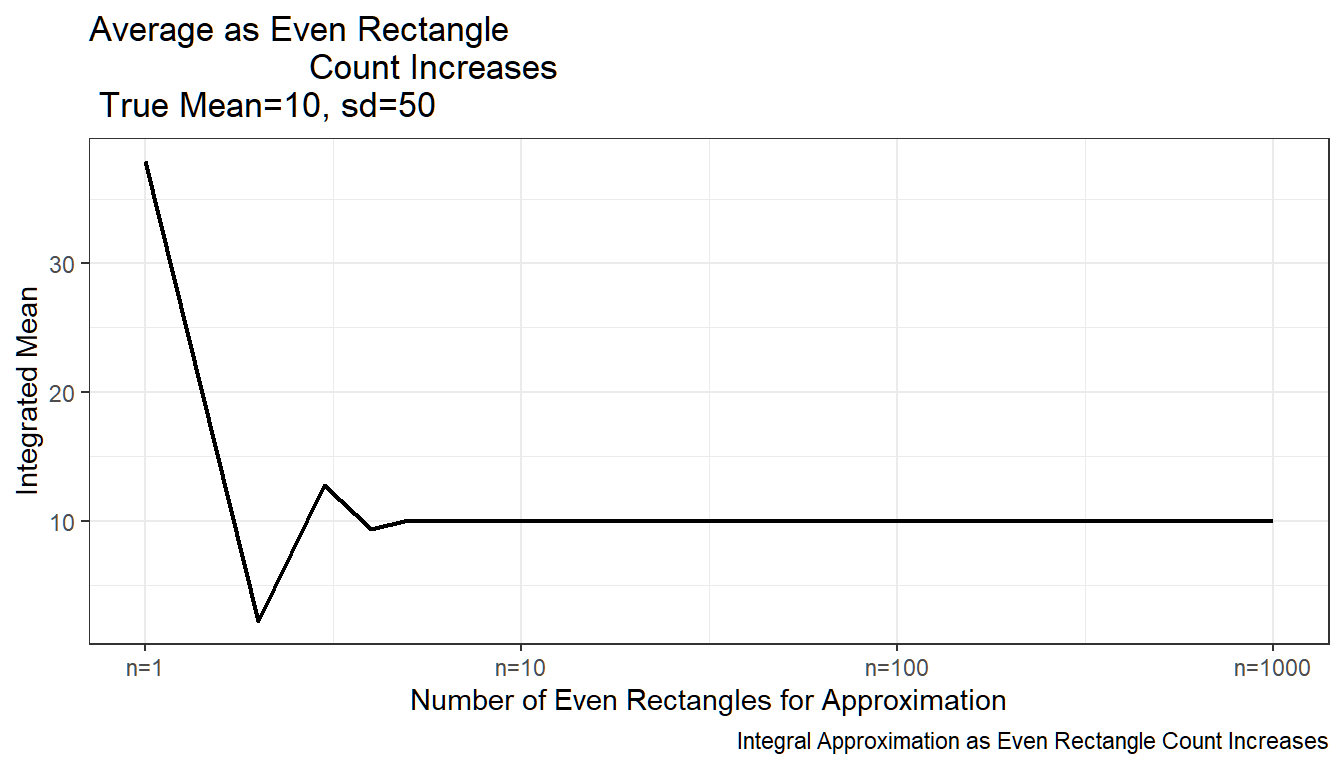
\includegraphics{Panel-Data-and-Optimization-with-R_files/figure-latex/unnamed-chunk-197-1} \end{center}

\hypertarget{additional-decomposition-testings}{%
\subsubsection{Additional Decomposition Testings}\label{additional-decomposition-testings}}

\begin{Shaded}
\begin{Highlighting}[]
\FunctionTok{head}\NormalTok{(df.decompose\_step2[vars.tomean.first],}\DecValTok{3}\NormalTok{)}
\FunctionTok{head}\NormalTok{(df.decompose\_step2[}\FunctionTok{paste0}\NormalTok{(vars.tomean.first, }\StringTok{\textquotesingle{}\_mean\textquotesingle{}}\NormalTok{)], }\DecValTok{3}\NormalTok{)}
\FunctionTok{head}\NormalTok{(df.coef[df.decompose\_step2}\SpecialCharTok{$}\NormalTok{variable,}
             \FunctionTok{paste0}\NormalTok{(vars.tomean.first, str.esti.suffix)], }\DecValTok{3}\NormalTok{)}
\NormalTok{df.decompose.tomean.first }\OtherTok{\textless{}{-}}\NormalTok{ df.decompose\_step2 }\SpecialCharTok{\%\textgreater{}\%}
    \FunctionTok{mutate}\NormalTok{(}\AttributeTok{pred\_new =}\NormalTok{ df.decompose\_step2}\SpecialCharTok{$}\NormalTok{value }\SpecialCharTok{+}
        \FunctionTok{rowSums}\NormalTok{((df.decompose\_step2[}\FunctionTok{paste0}\NormalTok{(vars.tomean.first, }\StringTok{\textquotesingle{}\_mean\textquotesingle{}}\NormalTok{)]}
                 \SpecialCharTok{{-}}\NormalTok{ df.decompose\_step2[vars.tomean.first])}
            \SpecialCharTok{*}\NormalTok{df.coef[df.decompose\_step2}\SpecialCharTok{$}\NormalTok{variable,}
                     \FunctionTok{paste0}\NormalTok{(vars.tomean.first, str.esti.suffix)])) }\SpecialCharTok{\%\textgreater{}\%}
        \FunctionTok{select}\NormalTok{(variable, value, pred\_new)}
\FunctionTok{head}\NormalTok{(df.decompose.tomean.first, }\DecValTok{10}\NormalTok{)}
\NormalTok{df.decompose.tomean.first }\SpecialCharTok{\%\textgreater{}\%}
        \FunctionTok{group\_by}\NormalTok{(variable) }\SpecialCharTok{\%\textgreater{}\%}
        \FunctionTok{summarize\_all}\NormalTok{(}\FunctionTok{funs}\NormalTok{(}\AttributeTok{mean =}\NormalTok{ mean, }\AttributeTok{sd =}\NormalTok{ sd))  }\SpecialCharTok{\%\textgreater{}\%}
  \FunctionTok{kable}\NormalTok{() }\SpecialCharTok{\%\textgreater{}\%}
  \FunctionTok{kable\_styling\_fc}\NormalTok{()}
\end{Highlighting}
\end{Shaded}

\begin{table}[!h]
\centering
\begin{tabular}{l|r|r|r|r}
\hline
variable & value\_mean & pred\_new\_mean & value\_sd & pred\_new\_sd\\
\hline
\cellcolor{gray!6}{hgt} & \cellcolor{gray!6}{73.41216} & \cellcolor{gray!6}{73.41216} & \cellcolor{gray!6}{4.675867} & \cellcolor{gray!6}{4.534947}\\
\hline
wgt & 8807.87656 & 8807.87656 & 1722.118824 & 1695.221845\\
\hline
\end{tabular}
\end{table}

Note the r-square from regression above matches up with the 1 - ratio below. This is the proper decomposition method that is equivalent to r2.

\begin{Shaded}
\begin{Highlighting}[]
\NormalTok{df.decompose\_step2 }\SpecialCharTok{\%\textgreater{}\%}
    \FunctionTok{mutate}\NormalTok{(}\AttributeTok{pred\_new =}\NormalTok{ df.decompose\_step2}\SpecialCharTok{$}\NormalTok{value }\SpecialCharTok{+}
        \FunctionTok{rowSums}\NormalTok{((df.decompose\_step2[}\FunctionTok{paste0}\NormalTok{(vars.tomean.second, }\StringTok{\textquotesingle{}\_mean\textquotesingle{}}\NormalTok{)]}
                 \SpecialCharTok{{-}}\NormalTok{ df.decompose\_step2[vars.tomean.second])}
            \SpecialCharTok{*}\NormalTok{df.coef[df.decompose\_step2}\SpecialCharTok{$}\NormalTok{variable,}
                     \FunctionTok{paste0}\NormalTok{(vars.tomean.second, str.esti.suffix)])) }\SpecialCharTok{\%\textgreater{}\%}
        \FunctionTok{select}\NormalTok{(variable, value, pred\_new) }\SpecialCharTok{\%\textgreater{}\%}
        \FunctionTok{group\_by}\NormalTok{(variable) }\SpecialCharTok{\%\textgreater{}\%}
        \FunctionTok{summarize\_all}\NormalTok{(}\FunctionTok{funs}\NormalTok{(}\AttributeTok{mean =}\NormalTok{ mean, }\AttributeTok{var =}\NormalTok{ var)) }\SpecialCharTok{\%\textgreater{}\%}
        \FunctionTok{mutate}\NormalTok{(}\AttributeTok{ratio =}\NormalTok{ (pred\_new\_var}\SpecialCharTok{/}\NormalTok{value\_var))  }\SpecialCharTok{\%\textgreater{}\%}
  \FunctionTok{kable}\NormalTok{() }\SpecialCharTok{\%\textgreater{}\%}
  \FunctionTok{kable\_styling\_fc}\NormalTok{()}
\end{Highlighting}
\end{Shaded}

\begin{table}[!h]
\centering
\begin{tabular}{l|r|r|r|r|r}
\hline
variable & value\_mean & pred\_new\_mean & value\_var & pred\_new\_var & ratio\\
\hline
\cellcolor{gray!6}{hgt} & \cellcolor{gray!6}{73.41216} & \cellcolor{gray!6}{73.41216} & \cellcolor{gray!6}{2.186374e+01} & \cellcolor{gray!6}{25.3504} & \cellcolor{gray!6}{1.1594724}\\
\hline
wgt & 8807.87656 & 8807.87656 & 2.965693e+06 & 2949187.6357 & 0.9944345\\
\hline
\end{tabular}
\end{table}

\hypertarget{nonlinear-and-other-regressions}{%
\chapter{Nonlinear and Other Regressions}\label{nonlinear-and-other-regressions}}

\hypertarget{logit-regression}{%
\section{Logit Regression}\label{logit-regression}}

\hypertarget{binary-logit}{%
\subsection{Binary Logit}\label{binary-logit}}

\begin{quote}
Go back to \href{http://fanwangecon.github.io/}{fan}'s \href{https://fanwangecon.github.io/REconTools/}{REconTools} Package, \href{https://fanwangecon.github.io/R4Econ/}{R Code Examples} Repository (\href{https://fanwangecon.github.io/R4Econ/bookdown}{bookdown site}), or \href{https://fanwangecon.github.io/Stat4Econ/}{Intro Stats with R} Repository (\href{https://fanwangecon.github.io/Stat4Econ/bookdown}{bookdown site}).
\end{quote}

\emph{Data Preparation}

\begin{Shaded}
\begin{Highlighting}[]
\NormalTok{df\_mtcars }\OtherTok{\textless{}{-}}\NormalTok{ mtcars}

\CommentTok{\# X{-}variables to use on RHS}
\NormalTok{ls\_st\_xs }\OtherTok{\textless{}{-}} \FunctionTok{c}\NormalTok{(}\StringTok{\textquotesingle{}mpg\textquotesingle{}}\NormalTok{, }\StringTok{\textquotesingle{}qsec\textquotesingle{}}\NormalTok{)}
\NormalTok{ls\_st\_xs }\OtherTok{\textless{}{-}} \FunctionTok{c}\NormalTok{(}\StringTok{\textquotesingle{}mpg\textquotesingle{}}\NormalTok{)}
\NormalTok{ls\_st\_xs }\OtherTok{\textless{}{-}} \FunctionTok{c}\NormalTok{(}\StringTok{\textquotesingle{}qsec\textquotesingle{}}\NormalTok{)}
\NormalTok{ls\_st\_xs }\OtherTok{\textless{}{-}} \FunctionTok{c}\NormalTok{(}\StringTok{\textquotesingle{}wt\textquotesingle{}}\NormalTok{)}
\NormalTok{ls\_st\_xs }\OtherTok{\textless{}{-}} \FunctionTok{c}\NormalTok{(}\StringTok{\textquotesingle{}mpg\textquotesingle{}}\NormalTok{, }\StringTok{\textquotesingle{}wt\textquotesingle{}}\NormalTok{, }\StringTok{\textquotesingle{}vs\textquotesingle{}}\NormalTok{)}

\NormalTok{svr\_binary }\OtherTok{\textless{}{-}} \StringTok{\textquotesingle{}hpLowHigh\textquotesingle{}}
\NormalTok{svr\_binary\_lb0 }\OtherTok{\textless{}{-}} \StringTok{\textquotesingle{}LowHP\textquotesingle{}}
\NormalTok{svr\_binary\_lb1 }\OtherTok{\textless{}{-}} \StringTok{\textquotesingle{}HighHP\textquotesingle{}}
\NormalTok{svr\_outcome }\OtherTok{\textless{}{-}} \StringTok{\textquotesingle{}am\textquotesingle{}}
\NormalTok{sdt\_name }\OtherTok{\textless{}{-}} \StringTok{\textquotesingle{}mtcars\textquotesingle{}}

\CommentTok{\# Discretize hp}
\NormalTok{df\_mtcars }\OtherTok{\textless{}{-}}\NormalTok{ df\_mtcars }\SpecialCharTok{\%\textgreater{}\%}
    \FunctionTok{mutate}\NormalTok{(}\SpecialCharTok{!!}\FunctionTok{sym}\NormalTok{(svr\_binary) }\SpecialCharTok{:}\ErrorTok{=} \FunctionTok{cut}\NormalTok{(hp,}
                           \AttributeTok{breaks=}\FunctionTok{c}\NormalTok{(}\SpecialCharTok{{-}}\ConstantTok{Inf}\NormalTok{, }\DecValTok{210}\NormalTok{, }\ConstantTok{Inf}\NormalTok{),}
                           \AttributeTok{labels=}\FunctionTok{c}\NormalTok{(svr\_binary\_lb0, svr\_binary\_lb1)))}
\end{Highlighting}
\end{Shaded}

\hypertarget{logit-regresion-and-prediction}{%
\subsubsection{Logit Regresion and Prediction}\label{logit-regresion-and-prediction}}

logit regression with glm, and predict using estimation data. Prediction and estimation with one variable.

\begin{itemize}
\tightlist
\item
  \href{https://stats.idre.ucla.edu/r/dae/logit-regression/}{LOGIT REGRESSION R DATA ANALYSIS EXAMPLES}
\item
  \href{https://www.statmethods.net/advstats/glm.html}{Generalized Linear Models}
\end{itemize}

\begin{Shaded}
\begin{Highlighting}[]
\CommentTok{\# Regress}
\NormalTok{rs\_logit }\OtherTok{\textless{}{-}} \FunctionTok{glm}\NormalTok{(}\FunctionTok{as.formula}\NormalTok{(}\FunctionTok{paste}\NormalTok{(svr\_outcome, }\StringTok{"\textasciitilde{}"}\NormalTok{, }\FunctionTok{paste}\NormalTok{(ls\_st\_xs, }\AttributeTok{collapse=}\StringTok{"+"}\NormalTok{)))}
\NormalTok{                ,}\AttributeTok{data =}\NormalTok{ df\_mtcars, }\AttributeTok{family =} \StringTok{"binomial"}\NormalTok{)}
\FunctionTok{summary}\NormalTok{(rs\_logit)}
\end{Highlighting}
\end{Shaded}

\begin{verbatim}
## 
## Call:
## glm(formula = as.formula(paste(svr_outcome, "~", paste(ls_st_xs, 
##     collapse = "+"))), family = "binomial", data = df_mtcars)
## 
## Deviance Residuals: 
##      Min        1Q    Median        3Q       Max  
## -1.73603  -0.25477  -0.04891   0.13402   1.90321  
## 
## Coefficients:
##             Estimate Std. Error z value Pr(>|z|)  
## (Intercept) 22.69008   13.95112   1.626   0.1039  
## mpg         -0.01786    0.33957  -0.053   0.9581  
## wt          -6.73804    3.01400  -2.236   0.0254 *
## vs          -4.44046    2.84247  -1.562   0.1182  
## ---
## Signif. codes:  0 '***' 0.001 '**' 0.01 '*' 0.05 '.' 0.1 ' ' 1
## 
## (Dispersion parameter for binomial family taken to be 1)
## 
##     Null deviance: 43.230  on 31  degrees of freedom
## Residual deviance: 13.092  on 28  degrees of freedom
## AIC: 21.092
## 
## Number of Fisher Scoring iterations: 7
\end{verbatim}

\begin{Shaded}
\begin{Highlighting}[]
\CommentTok{\# Predcit Using Regression Data}
\NormalTok{df\_mtcars}\SpecialCharTok{$}\NormalTok{p\_mpg }\OtherTok{\textless{}{-}} \FunctionTok{predict}\NormalTok{(rs\_logit, }\AttributeTok{newdata =}\NormalTok{ df\_mtcars, }\AttributeTok{type =} \StringTok{"response"}\NormalTok{)}
\end{Highlighting}
\end{Shaded}

\hypertarget{prediction-with-observed-binary-input}{%
\paragraph{Prediction with Observed Binary Input}\label{prediction-with-observed-binary-input}}

Logit regression with a continuous variable and a binary variable. Predict outcome with observed continuous variable as well as observed binary input variable.

\begin{Shaded}
\begin{Highlighting}[]
\CommentTok{\# Regress}
\NormalTok{rs\_logit\_bi }\OtherTok{\textless{}{-}} \FunctionTok{glm}\NormalTok{(}\FunctionTok{as.formula}\NormalTok{(}\FunctionTok{paste}\NormalTok{(svr\_outcome,}
                                    \StringTok{"\textasciitilde{} factor("}\NormalTok{, svr\_binary,}\StringTok{") + "}\NormalTok{,}
                                    \FunctionTok{paste}\NormalTok{(ls\_st\_xs, }\AttributeTok{collapse=}\StringTok{"+"}\NormalTok{)))}
\NormalTok{                   , }\AttributeTok{data =}\NormalTok{ df\_mtcars, }\AttributeTok{family =} \StringTok{"binomial"}\NormalTok{)}
\FunctionTok{summary}\NormalTok{(rs\_logit\_bi)}
\end{Highlighting}
\end{Shaded}

\begin{verbatim}
## 
## Call:
## glm(formula = as.formula(paste(svr_outcome, "~ factor(", svr_binary, 
##     ") + ", paste(ls_st_xs, collapse = "+"))), family = "binomial", 
##     data = df_mtcars)
## 
## Deviance Residuals: 
##      Min        1Q    Median        3Q       Max  
## -1.45771  -0.09563  -0.00875   0.00555   1.87612  
## 
## Coefficients:
##                         Estimate Std. Error z value Pr(>|z|)  
## (Intercept)               3.8285    18.0390   0.212   0.8319  
## factor(hpLowHigh)HighHP   6.9907     5.5176   1.267   0.2052  
## mpg                       0.8985     0.8906   1.009   0.3131  
## wt                       -6.7291     3.3166  -2.029   0.0425 *
## vs                       -5.9206     4.1908  -1.413   0.1577  
## ---
## Signif. codes:  0 '***' 0.001 '**' 0.01 '*' 0.05 '.' 0.1 ' ' 1
## 
## (Dispersion parameter for binomial family taken to be 1)
## 
##     Null deviance: 43.2297  on 31  degrees of freedom
## Residual deviance:  8.9777  on 27  degrees of freedom
## AIC: 18.978
## 
## Number of Fisher Scoring iterations: 9
\end{verbatim}

\begin{Shaded}
\begin{Highlighting}[]
\CommentTok{\# Predcit Using Regresion Data}
\NormalTok{df\_mtcars}\SpecialCharTok{$}\NormalTok{p\_mpg\_hp }\OtherTok{\textless{}{-}} \FunctionTok{predict}\NormalTok{(rs\_logit\_bi, }\AttributeTok{newdata =}\NormalTok{ df\_mtcars, }\AttributeTok{type =} \StringTok{"response"}\NormalTok{)}

\CommentTok{\# Predicted Probabilities am on mgp with or without hp binary}
\NormalTok{scatter }\OtherTok{\textless{}{-}} \FunctionTok{ggplot}\NormalTok{(df\_mtcars, }\FunctionTok{aes}\NormalTok{(}\AttributeTok{x=}\NormalTok{p\_mpg\_hp, }\AttributeTok{y=}\NormalTok{p\_mpg)) }\SpecialCharTok{+}
      \FunctionTok{geom\_point}\NormalTok{(}\AttributeTok{size=}\DecValTok{1}\NormalTok{) }\SpecialCharTok{+}
      \CommentTok{\# geom\_smooth(method=lm) + \# Trend line}
      \FunctionTok{geom\_abline}\NormalTok{(}\AttributeTok{intercept =} \DecValTok{0}\NormalTok{, }\AttributeTok{slope =} \DecValTok{1}\NormalTok{) }\SpecialCharTok{+} \CommentTok{\# 45 degree line}
      \FunctionTok{labs}\NormalTok{(}\AttributeTok{title =} \FunctionTok{paste0}\NormalTok{(}\StringTok{\textquotesingle{}Predicted Probabilities \textquotesingle{}}\NormalTok{, svr\_outcome, }\StringTok{\textquotesingle{} on \textquotesingle{}}\NormalTok{, ls\_st\_xs, }\StringTok{\textquotesingle{} with or without hp binary\textquotesingle{}}\NormalTok{),}
           \AttributeTok{x =} \FunctionTok{paste0}\NormalTok{(}\StringTok{\textquotesingle{}prediction with \textquotesingle{}}\NormalTok{, ls\_st\_xs, }\StringTok{\textquotesingle{} and binary \textquotesingle{}}\NormalTok{, svr\_binary, }\StringTok{\textquotesingle{} indicator, 1 is high\textquotesingle{}}\NormalTok{),}
           \AttributeTok{y =} \FunctionTok{paste0}\NormalTok{(}\StringTok{\textquotesingle{}prediction with only \textquotesingle{}}\NormalTok{, ls\_st\_xs),}
           \AttributeTok{caption =} \StringTok{\textquotesingle{}mtcars; prediction based on observed data\textquotesingle{}}\NormalTok{) }\SpecialCharTok{+}
      \FunctionTok{theme\_bw}\NormalTok{()}
\FunctionTok{print}\NormalTok{(scatter)}
\end{Highlighting}
\end{Shaded}

\begin{center}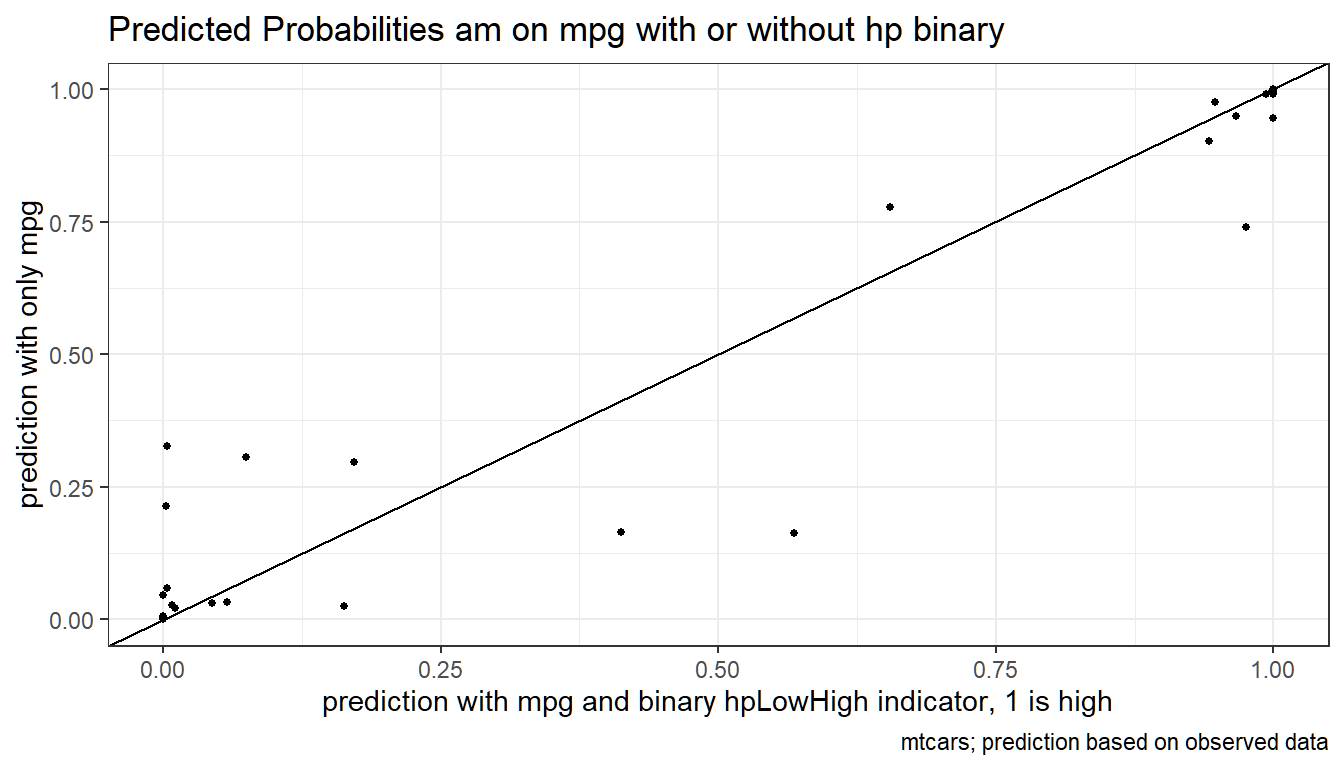
\includegraphics{Panel-Data-and-Optimization-with-R_files/figure-latex/logit with binary and continuous RHS-1} \end{center}

\hypertarget{prediction-with-binary-set-to-0-and-1}{%
\paragraph{Prediction with Binary set to 0 and 1}\label{prediction-with-binary-set-to-0-and-1}}

Now generate two predictions. One set where binary input is equal to 0, and another where the binary inputs are equal to 1. Ignore whether in data binary input is equal to 0 or 1. Use the same regression results as what was just derived.

Note that given the example here, the probability changes a lot when we

\begin{Shaded}
\begin{Highlighting}[]
\CommentTok{\# Previous regression results}
\FunctionTok{summary}\NormalTok{(rs\_logit\_bi)}
\end{Highlighting}
\end{Shaded}

\begin{verbatim}
## 
## Call:
## glm(formula = as.formula(paste(svr_outcome, "~ factor(", svr_binary, 
##     ") + ", paste(ls_st_xs, collapse = "+"))), family = "binomial", 
##     data = df_mtcars)
## 
## Deviance Residuals: 
##      Min        1Q    Median        3Q       Max  
## -1.45771  -0.09563  -0.00875   0.00555   1.87612  
## 
## Coefficients:
##                         Estimate Std. Error z value Pr(>|z|)  
## (Intercept)               3.8285    18.0390   0.212   0.8319  
## factor(hpLowHigh)HighHP   6.9907     5.5176   1.267   0.2052  
## mpg                       0.8985     0.8906   1.009   0.3131  
## wt                       -6.7291     3.3166  -2.029   0.0425 *
## vs                       -5.9206     4.1908  -1.413   0.1577  
## ---
## Signif. codes:  0 '***' 0.001 '**' 0.01 '*' 0.05 '.' 0.1 ' ' 1
## 
## (Dispersion parameter for binomial family taken to be 1)
## 
##     Null deviance: 43.2297  on 31  degrees of freedom
## Residual deviance:  8.9777  on 27  degrees of freedom
## AIC: 18.978
## 
## Number of Fisher Scoring iterations: 9
\end{verbatim}

\begin{Shaded}
\begin{Highlighting}[]
\CommentTok{\# Two different dataframes, mutate the binary regressor}
\NormalTok{df\_mtcars\_bi0 }\OtherTok{\textless{}{-}}\NormalTok{ df\_mtcars }\SpecialCharTok{\%\textgreater{}\%} \FunctionTok{mutate}\NormalTok{(}\SpecialCharTok{!!}\FunctionTok{sym}\NormalTok{(svr\_binary) }\SpecialCharTok{:}\ErrorTok{=}\NormalTok{ svr\_binary\_lb0)}
\NormalTok{df\_mtcars\_bi1 }\OtherTok{\textless{}{-}}\NormalTok{ df\_mtcars }\SpecialCharTok{\%\textgreater{}\%} \FunctionTok{mutate}\NormalTok{(}\SpecialCharTok{!!}\FunctionTok{sym}\NormalTok{(svr\_binary) }\SpecialCharTok{:}\ErrorTok{=}\NormalTok{ svr\_binary\_lb1)}

\CommentTok{\# Predcit Using Regresion Data}
\NormalTok{df\_mtcars}\SpecialCharTok{$}\NormalTok{p\_mpg\_hp\_bi0 }\OtherTok{\textless{}{-}} \FunctionTok{predict}\NormalTok{(rs\_logit\_bi, }\AttributeTok{newdata =}\NormalTok{ df\_mtcars\_bi0, }\AttributeTok{type =} \StringTok{"response"}\NormalTok{)}
\NormalTok{df\_mtcars}\SpecialCharTok{$}\NormalTok{p\_mpg\_hp\_bi1 }\OtherTok{\textless{}{-}} \FunctionTok{predict}\NormalTok{(rs\_logit\_bi, }\AttributeTok{newdata =}\NormalTok{ df\_mtcars\_bi1, }\AttributeTok{type =} \StringTok{"response"}\NormalTok{)}

\CommentTok{\# Predicted Probabilities and Binary Input}
\NormalTok{scatter }\OtherTok{\textless{}{-}} \FunctionTok{ggplot}\NormalTok{(df\_mtcars, }\FunctionTok{aes}\NormalTok{(}\AttributeTok{x=}\NormalTok{p\_mpg\_hp\_bi0)) }\SpecialCharTok{+}
      \FunctionTok{geom\_point}\NormalTok{(}\FunctionTok{aes}\NormalTok{(}\AttributeTok{y=}\NormalTok{p\_mpg\_hp), }\AttributeTok{size=}\DecValTok{4}\NormalTok{, }\AttributeTok{shape=}\DecValTok{4}\NormalTok{, }\AttributeTok{color=}\StringTok{"red"}\NormalTok{) }\SpecialCharTok{+}
      \FunctionTok{geom\_point}\NormalTok{(}\FunctionTok{aes}\NormalTok{(}\AttributeTok{y=}\NormalTok{p\_mpg\_hp\_bi1), }\AttributeTok{size=}\DecValTok{2}\NormalTok{, }\AttributeTok{shape=}\DecValTok{8}\NormalTok{) }\SpecialCharTok{+}
      \CommentTok{\# geom\_smooth(method=lm) + \# Trend line}
      \FunctionTok{geom\_abline}\NormalTok{(}\AttributeTok{intercept =} \DecValTok{0}\NormalTok{, }\AttributeTok{slope =} \DecValTok{1}\NormalTok{) }\SpecialCharTok{+} \CommentTok{\# 45 degree line}
      \FunctionTok{labs}\NormalTok{(}\AttributeTok{title =} \FunctionTok{paste0}\NormalTok{(}\StringTok{\textquotesingle{}Predicted Probabilities and Binary Input\textquotesingle{}}\NormalTok{,}
                          \StringTok{\textquotesingle{}}\SpecialCharTok{\textbackslash{}n}\StringTok{cross(shape=4)/red is predict actual binary data\textquotesingle{}}\NormalTok{,}
                          \StringTok{\textquotesingle{}}\SpecialCharTok{\textbackslash{}n}\StringTok{star(shape=8)/black is predict set binary = 1 for all\textquotesingle{}}\NormalTok{),}
            \AttributeTok{x =} \FunctionTok{paste0}\NormalTok{(}\StringTok{\textquotesingle{}prediction with \textquotesingle{}}\NormalTok{, ls\_st\_xs, }\StringTok{\textquotesingle{} and binary \textquotesingle{}}\NormalTok{, svr\_binary, }\StringTok{\textquotesingle{} = 0 for all\textquotesingle{}}\NormalTok{),}
            \AttributeTok{y =} \FunctionTok{paste0}\NormalTok{(}\StringTok{\textquotesingle{}prediction with \textquotesingle{}}\NormalTok{, ls\_st\_xs, }\StringTok{\textquotesingle{} and binary \textquotesingle{}}\NormalTok{, svr\_binary, }\StringTok{\textquotesingle{} = 1\textquotesingle{}}\NormalTok{),}
           \AttributeTok{caption =} \FunctionTok{paste0}\NormalTok{(sdt\_name)) }\SpecialCharTok{+}
      \FunctionTok{theme\_bw}\NormalTok{()}
\FunctionTok{print}\NormalTok{(scatter)}
\end{Highlighting}
\end{Shaded}

\begin{center}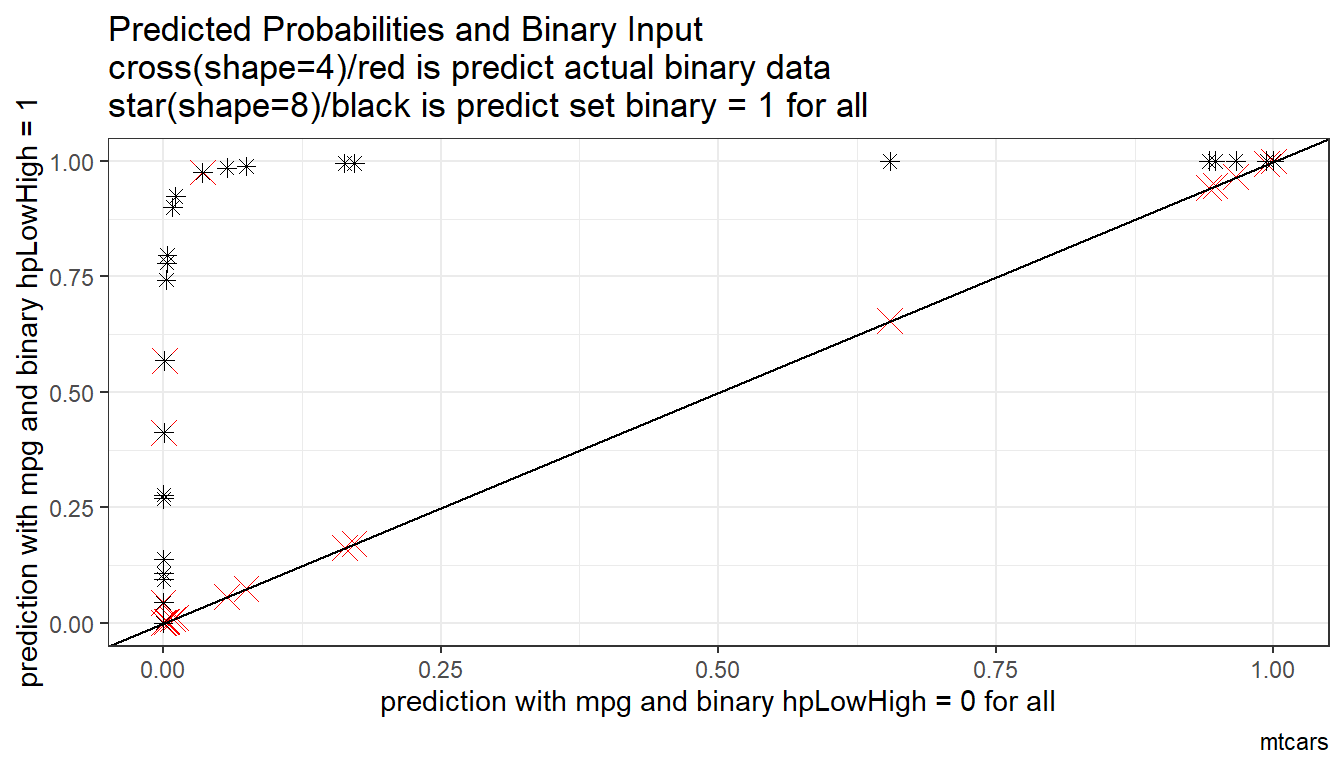
\includegraphics{Panel-Data-and-Optimization-with-R_files/figure-latex/logit prediction 0 vs 1-1} \end{center}

\hypertarget{prediction-with-binary-set-to-0-and-1-difference}{%
\paragraph{Prediction with Binary set to 0 and 1 Difference}\label{prediction-with-binary-set-to-0-and-1-difference}}

What is the difference in probability between binary = 0 vs binary = 1. How does that relate to the probability of outcome of interest when binary = 0 for all.

In the binary logit case, the relationship will be hump--shaped by construction between \(A_i\) and \(\alpha_i\). In the exponential wage cases, the relationship is convex upwards.

\begin{Shaded}
\begin{Highlighting}[]
\CommentTok{\# Generate Gap Variable}
\NormalTok{df\_mtcars }\OtherTok{\textless{}{-}}\NormalTok{ df\_mtcars }\SpecialCharTok{\%\textgreater{}\%} \FunctionTok{mutate}\NormalTok{(}\AttributeTok{alpha\_i =}\NormalTok{ p\_mpg\_hp\_bi1 }\SpecialCharTok{{-}}\NormalTok{ p\_mpg\_hp\_bi0) }\SpecialCharTok{\%\textgreater{}\%}
                \FunctionTok{mutate}\NormalTok{(}\AttributeTok{A\_i =}\NormalTok{ p\_mpg\_hp\_bi0)}

\CommentTok{\# Binary Marginal Effects and Prediction without Binary}
\NormalTok{scatter }\OtherTok{\textless{}{-}} \FunctionTok{ggplot}\NormalTok{(df\_mtcars, }\FunctionTok{aes}\NormalTok{(}\AttributeTok{x=}\NormalTok{A\_i)) }\SpecialCharTok{+}
      \FunctionTok{geom\_point}\NormalTok{(}\FunctionTok{aes}\NormalTok{(}\AttributeTok{y=}\NormalTok{alpha\_i), }\AttributeTok{size=}\DecValTok{4}\NormalTok{, }\AttributeTok{shape=}\DecValTok{4}\NormalTok{, }\AttributeTok{color=}\StringTok{"red"}\NormalTok{) }\SpecialCharTok{+}
      \FunctionTok{geom\_abline}\NormalTok{(}\AttributeTok{intercept =} \DecValTok{0}\NormalTok{, }\AttributeTok{slope =} \DecValTok{1}\NormalTok{) }\SpecialCharTok{+} \CommentTok{\# 45 degree line}
      \FunctionTok{labs}\NormalTok{(}\AttributeTok{title =} \FunctionTok{paste0}\NormalTok{(}\StringTok{\textquotesingle{}Binary Marginal Effects and Prediction without Binary\textquotesingle{}}\NormalTok{),}
           \AttributeTok{x =} \StringTok{\textquotesingle{}P(binary=0) for all\textquotesingle{}}\NormalTok{,}
           \AttributeTok{y =} \StringTok{\textquotesingle{}P(binary=1) {-} P(binary=0) gap\textquotesingle{}}\NormalTok{,}
           \AttributeTok{caption =} \FunctionTok{paste0}\NormalTok{(sdt\_name)) }\SpecialCharTok{+}
      \FunctionTok{theme\_bw}\NormalTok{()}
\FunctionTok{print}\NormalTok{(scatter)}
\end{Highlighting}
\end{Shaded}

\begin{center}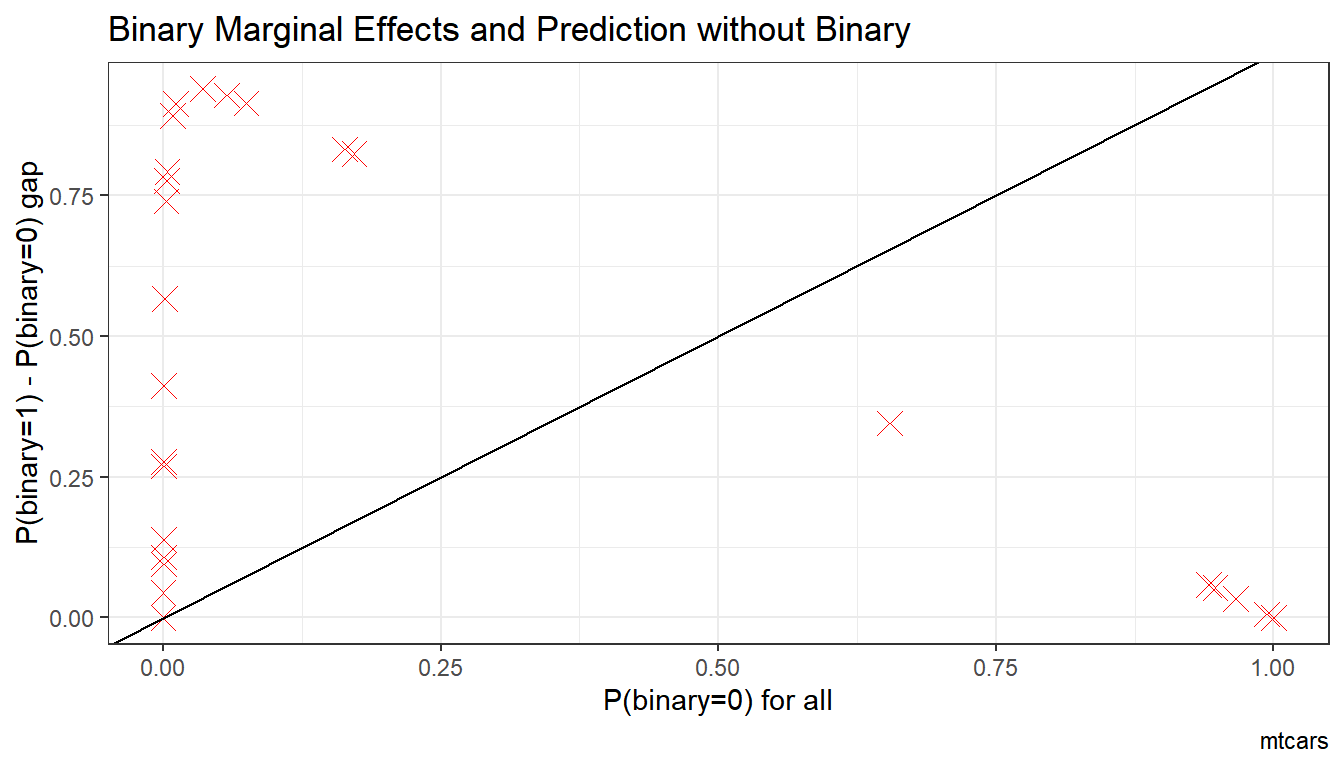
\includegraphics{Panel-Data-and-Optimization-with-R_files/figure-latex/logit prediction marginal vs base-1} \end{center}

\hypertarget{x-variables-and-a-and-alpha}{%
\paragraph{X variables and A and alpha}\label{x-variables-and-a-and-alpha}}

Given the x-variables included in the logit regression, how do they relate to A\_i and alpha\_i

\begin{Shaded}
\begin{Highlighting}[]
\CommentTok{\# Generate Gap Variable}
\NormalTok{df\_mtcars }\OtherTok{\textless{}{-}}\NormalTok{ df\_mtcars }\SpecialCharTok{\%\textgreater{}\%} \FunctionTok{mutate}\NormalTok{(}\AttributeTok{alpha\_i =}\NormalTok{ p\_mpg\_hp\_bi1 }\SpecialCharTok{{-}}\NormalTok{ p\_mpg\_hp\_bi0) }\SpecialCharTok{\%\textgreater{}\%}
                \FunctionTok{mutate}\NormalTok{(}\AttributeTok{A\_i =}\NormalTok{ p\_mpg\_hp\_bi0)}

\CommentTok{\# Binary Marginal Effects and Prediction without Binary}
\NormalTok{ggplot.A.alpha.x }\OtherTok{\textless{}{-}} \ControlFlowTok{function}\NormalTok{(svr\_x, df,}
                             \AttributeTok{svr\_alpha =} \StringTok{\textquotesingle{}alpha\_i\textquotesingle{}}\NormalTok{, }\AttributeTok{svr\_A =} \StringTok{"A\_i"}\NormalTok{)\{}

\NormalTok{  scatter }\OtherTok{\textless{}{-}} \FunctionTok{ggplot}\NormalTok{(df, }\FunctionTok{aes}\NormalTok{(}\AttributeTok{x=}\SpecialCharTok{!!}\FunctionTok{sym}\NormalTok{(svr\_x))) }\SpecialCharTok{+}
        \FunctionTok{geom\_point}\NormalTok{(}\FunctionTok{aes}\NormalTok{(}\AttributeTok{y=}\NormalTok{alpha\_i), }\AttributeTok{size=}\DecValTok{4}\NormalTok{, }\AttributeTok{shape=}\DecValTok{4}\NormalTok{, }\AttributeTok{color=}\StringTok{"red"}\NormalTok{) }\SpecialCharTok{+}
        \FunctionTok{geom\_point}\NormalTok{(}\FunctionTok{aes}\NormalTok{(}\AttributeTok{y=}\NormalTok{A\_i), }\AttributeTok{size=}\DecValTok{2}\NormalTok{, }\AttributeTok{shape=}\DecValTok{8}\NormalTok{, }\AttributeTok{color=}\StringTok{"blue"}\NormalTok{) }\SpecialCharTok{+}
        \FunctionTok{geom\_abline}\NormalTok{(}\AttributeTok{intercept =} \DecValTok{0}\NormalTok{, }\AttributeTok{slope =} \DecValTok{1}\NormalTok{) }\SpecialCharTok{+} \CommentTok{\# 45 degree line}
        \FunctionTok{labs}\NormalTok{(}\AttributeTok{title =} \FunctionTok{paste0}\NormalTok{(}\StringTok{\textquotesingle{}A (blue) and alpha (red) vs x variables=\textquotesingle{}}\NormalTok{, svr\_x),}
             \AttributeTok{x =}\NormalTok{ svr\_x,}
             \AttributeTok{y =} \StringTok{\textquotesingle{}Probabilities\textquotesingle{}}\NormalTok{,}
             \AttributeTok{caption =} \FunctionTok{paste0}\NormalTok{(sdt\_name)) }\SpecialCharTok{+}
        \FunctionTok{theme\_bw}\NormalTok{()}

\FunctionTok{return}\NormalTok{(scatter)}
\NormalTok{\}}

\CommentTok{\# Plot over multiple}
\FunctionTok{lapply}\NormalTok{(ls\_st\_xs,}
\NormalTok{       ggplot.A.alpha.x,}
       \AttributeTok{df =}\NormalTok{ df\_mtcars)}
\end{Highlighting}
\end{Shaded}

\begin{verbatim}
## [[1]]
\end{verbatim}

\begin{center}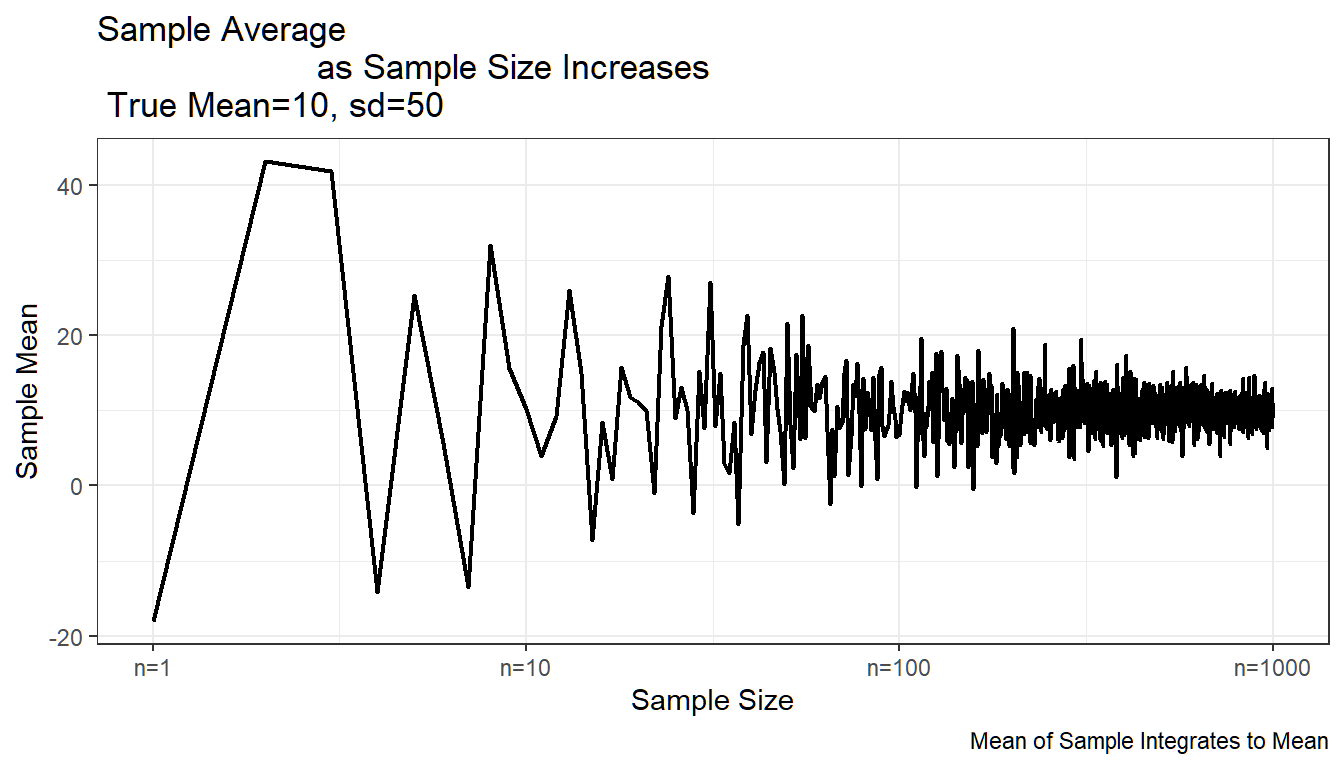
\includegraphics{Panel-Data-and-Optimization-with-R_files/figure-latex/unnamed-chunk-201-1} \end{center}

\begin{verbatim}
## 
## [[2]]
\end{verbatim}

\begin{center}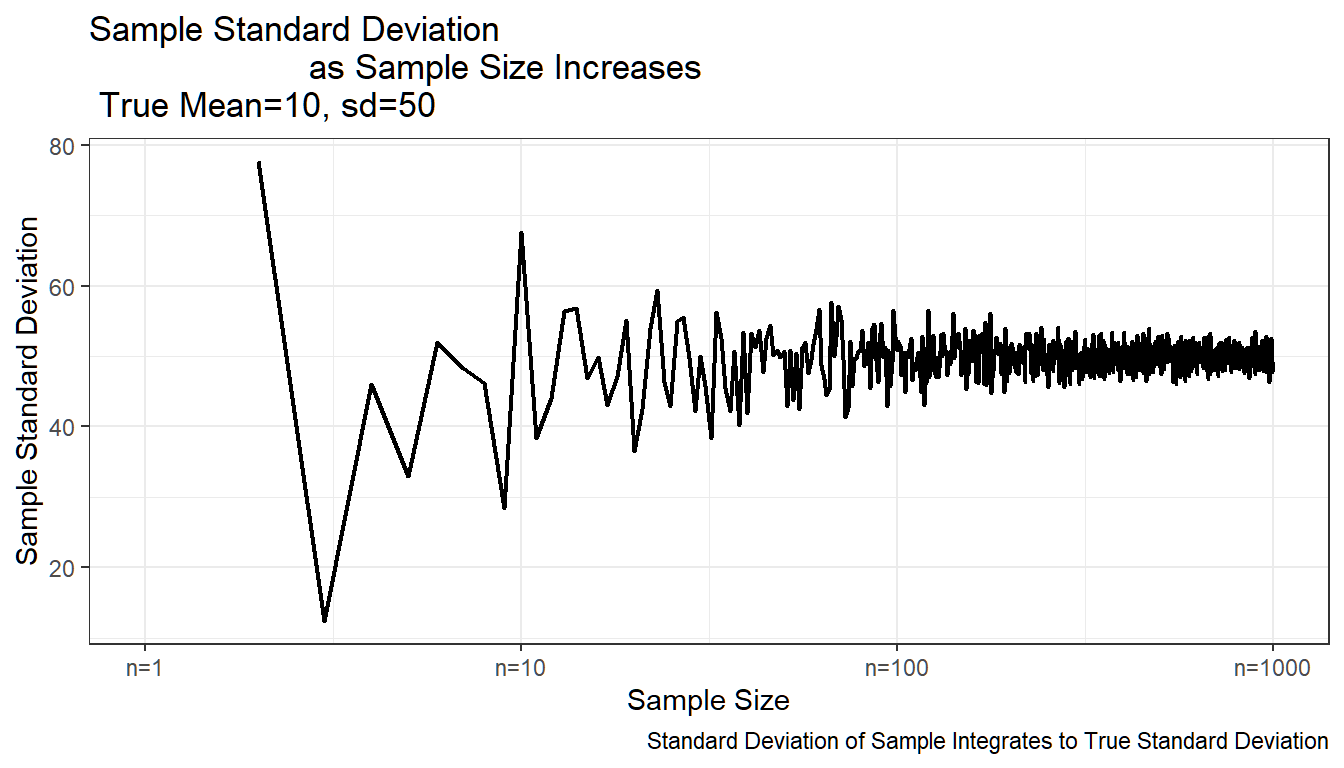
\includegraphics{Panel-Data-and-Optimization-with-R_files/figure-latex/unnamed-chunk-201-2} \end{center}

\begin{verbatim}
## 
## [[3]]
\end{verbatim}

\begin{center}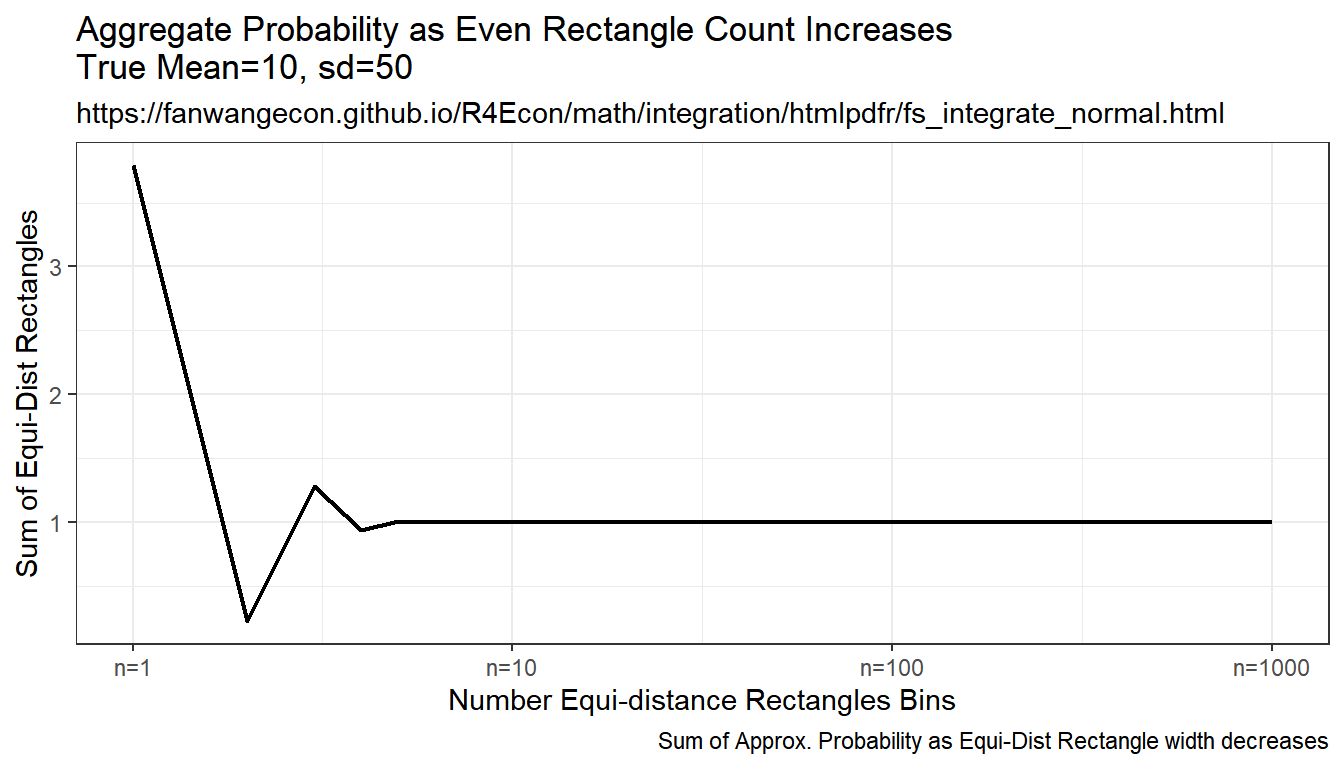
\includegraphics{Panel-Data-and-Optimization-with-R_files/figure-latex/unnamed-chunk-201-3} \end{center}

\hypertarget{quantile-regression}{%
\section{Quantile Regression}\label{quantile-regression}}

\hypertarget{quantile-regression-basics}{%
\subsection{Quantile Regression Basics}\label{quantile-regression-basics}}

\begin{quote}
Go back to \href{http://fanwangecon.github.io/}{fan}'s \href{https://fanwangecon.github.io/REconTools/}{REconTools} Package, \href{https://fanwangecon.github.io/R4Econ/}{R Code Examples} Repository (\href{https://fanwangecon.github.io/R4Econ/bookdown}{bookdown site}), or \href{https://fanwangecon.github.io/Stat4Econ/}{Intro Stats with R} Repository (\href{https://fanwangecon.github.io/Stat4Econ/bookdown}{bookdown site}).
\end{quote}

\hypertarget{estimate-mean-and-conditional-quantile-coefficients-using-mtcars-dataset}{%
\subsubsection{Estimate Mean and Conditional Quantile Coefficients using mtcars dataset}\label{estimate-mean-and-conditional-quantile-coefficients-using-mtcars-dataset}}

Here, we conduct tests for using the \href{https://cran.r-project.org/web/packages/quantreg/index.html}{quantreg} package, using the built-in \href{https://stat.ethz.ch/R-manual/R-devel/library/datasets/html/mtcars.html}{mtcars} dataset.

First, estimate the mean (OLS) regression:

\begin{Shaded}
\begin{Highlighting}[]
\NormalTok{fit\_mean }\OtherTok{\textless{}{-}} \FunctionTok{lm}\NormalTok{(mpg }\SpecialCharTok{\textasciitilde{}}\NormalTok{ disp }\SpecialCharTok{+}\NormalTok{ hp }\SpecialCharTok{+} \FunctionTok{factor}\NormalTok{(am) }\SpecialCharTok{+} \FunctionTok{factor}\NormalTok{(vs), }\AttributeTok{data =}\NormalTok{ mtcars)}
\FunctionTok{summary}\NormalTok{(fit\_mean)}
\end{Highlighting}
\end{Shaded}

\begin{verbatim}
## 
## Call:
## lm(formula = mpg ~ disp + hp + factor(am) + factor(vs), data = mtcars)
## 
## Residuals:
##     Min      1Q  Median      3Q     Max 
## -4.7981 -1.9532  0.0111  1.5665  5.6321 
## 
## Coefficients:
##              Estimate Std. Error t value Pr(>|t|)    
## (Intercept) 24.832119   2.890418   8.591 3.32e-09 ***
## disp        -0.008304   0.010087  -0.823  0.41757    
## hp          -0.037623   0.013846  -2.717  0.01135 *  
## factor(am)1  4.419257   1.493243   2.960  0.00634 ** 
## factor(vs)1  2.052472   1.627096   1.261  0.21794    
## ---
## Signif. codes:  0 '***' 0.001 '**' 0.01 '*' 0.05 '.' 0.1 ' ' 1
## 
## Residual standard error: 2.812 on 27 degrees of freedom
## Multiple R-squared:  0.8104, Adjusted R-squared:  0.7823 
## F-statistic: 28.85 on 4 and 27 DF,  p-value: 2.13e-09
\end{verbatim}

Now estimate conditional quantile regressions (not that this remains linear) at various quantiles, standard error obtained via bootstrap. Note that there is a gradient in the quantile hp coefficients as well as disp. disp sign reverses, also the coefficient on factor am is different by quantiles:

\begin{Shaded}
\begin{Highlighting}[]
\NormalTok{ls\_fl\_quantiles }\OtherTok{\textless{}{-}} \FunctionTok{c}\NormalTok{(}\FloatTok{0.25}\NormalTok{, }\FloatTok{0.50}\NormalTok{, }\FloatTok{0.75}\NormalTok{)}
\NormalTok{fit\_quantiles }\OtherTok{\textless{}{-}} \FunctionTok{rq}\NormalTok{(mpg }\SpecialCharTok{\textasciitilde{}}\NormalTok{ disp }\SpecialCharTok{+}\NormalTok{ hp }\SpecialCharTok{+} \FunctionTok{factor}\NormalTok{(am),}
               \AttributeTok{tau =}\NormalTok{ ls\_fl\_quantiles,}
               \AttributeTok{data =}\NormalTok{ mtcars)}
\FunctionTok{summary}\NormalTok{(fit\_quantiles, }\AttributeTok{se =} \StringTok{"boot"}\NormalTok{)}
\end{Highlighting}
\end{Shaded}

\begin{verbatim}
## 
## Call: rq(formula = mpg ~ disp + hp + factor(am), tau = ls_fl_quantiles, 
##     data = mtcars)
## 
## tau: [1] 0.25
## 
## Coefficients:
##             Value    Std. Error t value  Pr(>|t|)
## (Intercept) 25.34665  1.38870   18.25209  0.00000
## disp        -0.02441  0.00798   -3.06028  0.00484
## hp          -0.01672  0.01409   -1.18621  0.24551
## factor(am)1  1.39719  1.41689    0.98610  0.33253
## 
## Call: rq(formula = mpg ~ disp + hp + factor(am), tau = ls_fl_quantiles, 
##     data = mtcars)
## 
## tau: [1] 0.5
## 
## Coefficients:
##             Value    Std. Error t value  Pr(>|t|)
## (Intercept) 27.49722  1.75659   15.65379  0.00000
## disp        -0.02253  0.01634   -1.37904  0.17880
## hp          -0.02713  0.02414   -1.12386  0.27062
## factor(am)1  3.37328  2.25738    1.49434  0.14627
## 
## Call: rq(formula = mpg ~ disp + hp + factor(am), tau = ls_fl_quantiles, 
##     data = mtcars)
## 
## tau: [1] 0.75
## 
## Coefficients:
##             Value    Std. Error t value  Pr(>|t|)
## (Intercept) 28.06384  1.68640   16.64124  0.00000
## disp         0.00445  0.01457    0.30566  0.76212
## hp          -0.06662  0.01795   -3.71247  0.00090
## factor(am)1  7.91402  2.36999    3.33926  0.00239
\end{verbatim}

\hypertarget{test-conditional-quantile-coefficients-if-different}{%
\subsubsection{Test Conditional Quantile Coefficients if Different}\label{test-conditional-quantile-coefficients-if-different}}

Use the rq.anova function frm the quantile regression packge to conduct WALD test. Remember WALD test says given unrestricted model's estimates, test where null is that the coefficients satisfy some linear restrictions.

To test, use the returned object from running rq with different numbers of quantiles, and set the option \emph{joint} to true or false. When joint is true: ``equality of slopes should be done as joint tests on all slope parameters'', when joint is false: ``separate tests on each of the slope parameters should be reported''. A slope parameter refers to one of the RHS variables.

Note that quantile tests are ``parallel line'' tests. Meaning that we should except to have different x-intercepts for each quantile, because they represents the levels of the conditional shocks distributions. However, if quantile coefficients for the slopes are all the same, then there are no quantile specific effects, mean effects would be sufficient.

see:

\begin{itemize}
\tightlist
\item
  \href{https://stackoverflow.com/questions/32743758/anova-rq-in-quantreg-package-in-r}{anova.rq() in quantreg package in R}
\end{itemize}

\hypertarget{test-statistical-difference-between-25th-and-50th-conditional-quantiles}{%
\paragraph{Test Statistical Difference between 25th and 50th Conditional Quantiles}\label{test-statistical-difference-between-25th-and-50th-conditional-quantiles}}

Given the quantile estimates above, the difference between 0.25 and 0.50 quantiles exists, but are they sufficiently large to be statistically different? What is the p-value? Reviewing the results below, they are not statistically different.

First, joint = TRUE. This is not testing if the coefficien on disp is the same as the coefficient on hp. This is testing jointly if the coefficients for different quantiles of disp, and different quantiles of hp are the same for each RHS variable.

\begin{Shaded}
\begin{Highlighting}[]
\NormalTok{ls\_fl\_quantiles }\OtherTok{\textless{}{-}} \FunctionTok{c}\NormalTok{(}\FloatTok{0.25}\NormalTok{, }\FloatTok{0.50}\NormalTok{)}
\NormalTok{fit\_quantiles }\OtherTok{\textless{}{-}} \FunctionTok{rq}\NormalTok{(mpg }\SpecialCharTok{\textasciitilde{}}\NormalTok{ disp }\SpecialCharTok{+}\NormalTok{ hp }\SpecialCharTok{+} \FunctionTok{factor}\NormalTok{(am),}
               \AttributeTok{tau =}\NormalTok{ ls\_fl\_quantiles,}
               \AttributeTok{data =}\NormalTok{ mtcars)}
\FunctionTok{anova}\NormalTok{(fit\_quantiles, }\AttributeTok{test =} \StringTok{"Wald"}\NormalTok{, }\AttributeTok{joint=}\ConstantTok{TRUE}\NormalTok{)}
\end{Highlighting}
\end{Shaded}

\begin{verbatim}
## Quantile Regression Analysis of Deviance Table
## 
## Model: mpg ~ disp + hp + factor(am)
## Joint Test of Equality of Slopes: tau in {  0.25 0.5  }
## 
##   Df Resid Df F value Pr(>F)
## 1  3       61  0.7986 0.4994
\end{verbatim}

Second, joint = False:

\begin{Shaded}
\begin{Highlighting}[]
\FunctionTok{anova}\NormalTok{(fit\_quantiles, }\AttributeTok{test =} \StringTok{"Wald"}\NormalTok{, }\AttributeTok{joint=}\ConstantTok{FALSE}\NormalTok{)}
\end{Highlighting}
\end{Shaded}

\begin{verbatim}
## Quantile Regression Analysis of Deviance Table
## 
## Model: mpg ~ disp + hp + factor(am)
## Tests of Equality of Distinct Slopes: tau in {  0.25 0.5  }
## 
##             Df Resid Df F value Pr(>F)
## disp         1       63  0.0304 0.8621
## hp           1       63  0.5397 0.4653
## factor(am)1  1       63  1.0957 0.2992
\end{verbatim}

\hypertarget{test-statistical-difference-between-25th-50th-and-75th-conditional-quantiles}{%
\paragraph{Test Statistical Difference between 25th, 50th, and 75th Conditional Quantiles}\label{test-statistical-difference-between-25th-50th-and-75th-conditional-quantiles}}

The 1st quartile and median do not seem to be statistically different, now include the 3rd quartile. As seen earlier, the quartiles jointly show a gradient. Now, we can see that idisp, hp and am are separately have statistically different

First, joint = TRUE:

\begin{Shaded}
\begin{Highlighting}[]
\NormalTok{ls\_fl\_quantiles }\OtherTok{\textless{}{-}} \FunctionTok{c}\NormalTok{(}\FloatTok{0.25}\NormalTok{, }\FloatTok{0.50}\NormalTok{, }\FloatTok{0.75}\NormalTok{)}
\NormalTok{fit\_quantiles }\OtherTok{\textless{}{-}} \FunctionTok{rq}\NormalTok{(mpg }\SpecialCharTok{\textasciitilde{}}\NormalTok{ disp }\SpecialCharTok{+}\NormalTok{ hp }\SpecialCharTok{+} \FunctionTok{factor}\NormalTok{(am),}
               \AttributeTok{tau =}\NormalTok{ ls\_fl\_quantiles,}
               \AttributeTok{data =}\NormalTok{ mtcars)}
\FunctionTok{anova}\NormalTok{(fit\_quantiles, }\AttributeTok{test =} \StringTok{"Wald"}\NormalTok{, }\AttributeTok{joint=}\ConstantTok{TRUE}\NormalTok{)}
\end{Highlighting}
\end{Shaded}

\begin{verbatim}
## Quantile Regression Analysis of Deviance Table
## 
## Model: mpg ~ disp + hp + factor(am)
## Joint Test of Equality of Slopes: tau in {  0.25 0.5 0.75  }
## 
##   Df Resid Df F value   Pr(>F)   
## 1  6       90   3.957 0.001475 **
## ---
## Signif. codes:  0 '***' 0.001 '**' 0.01 '*' 0.05 '.' 0.1 ' ' 1
\end{verbatim}

Second, joint = False:

\begin{Shaded}
\begin{Highlighting}[]
\FunctionTok{anova}\NormalTok{(fit\_quantiles, }\AttributeTok{test =} \StringTok{"Wald"}\NormalTok{, }\AttributeTok{joint=}\ConstantTok{FALSE}\NormalTok{)}
\end{Highlighting}
\end{Shaded}

\begin{verbatim}
## Quantile Regression Analysis of Deviance Table
## 
## Model: mpg ~ disp + hp + factor(am)
## Tests of Equality of Distinct Slopes: tau in {  0.25 0.5 0.75  }
## 
##             Df Resid Df F value    Pr(>F)    
## disp         2       94  9.2284 0.0002191 ***
## hp           2       94  6.5798 0.0021162 ** 
## factor(am)1  2       94  3.6669 0.0292803 *  
## ---
## Signif. codes:  0 '***' 0.001 '**' 0.01 '*' 0.05 '.' 0.1 ' ' 1
\end{verbatim}

\hypertarget{optimization}{%
\chapter{Optimization}\label{optimization}}

\hypertarget{bisection}{%
\section{Bisection}\label{bisection}}

\hypertarget{bisection-1}{%
\subsection{Bisection}\label{bisection-1}}

\begin{quote}
Go back to \href{http://fanwangecon.github.io/}{fan}'s \href{https://fanwangecon.github.io/REconTools/}{REconTools} Package, \href{https://fanwangecon.github.io/R4Econ/}{R Code Examples} Repository (\href{https://fanwangecon.github.io/R4Econ/bookdown}{bookdown site}), or \href{https://fanwangecon.github.io/Stat4Econ/}{Intro Stats with R} Repository (\href{https://fanwangecon.github.io/Stat4Econ/bookdown}{bookdown site}).
\end{quote}

See the \href{https://fanwangecon.github.io/REconTools/reference/ff_opti_bisect_pmap_multi.html}{ff\_opti\_bisect\_pmap\_multi} function from \href{https://fanwangecon.github.io/}{Fan}'s \emph{\href{https://fanwangecon.github.io/REconTools/}{REconTools}} Package, which provides a resuable function based on the algorithm worked out here.

The bisection specific code does not need to do much.

\begin{itemize}
\tightlist
\item
  list variables in file for grouping, each group is an individual for whom we want to calculate optimal choice for using bisection.
\item
  string variable name of input where functions are evaluated, these are already contained in the dataframe, existing variable names, row specific, rowwise computation over these, each rowwise calculation using different rows.
\item
  scalar and array values that are applied to every rowwise calculation, all rowwise calculations using the same scalars and arrays.
\item
  string output variable name
\end{itemize}

This is how I implement the bisection algorithm, when we know the bounding minimum and maximum to be below and above zero already.

\begin{enumerate}
\def\labelenumi{\arabic{enumi}.}
\tightlist
\item
  Evaluate \(f^0_a = f(a^0)\) and \(f^0_b = f(b^0)\), min and max points.
\item
  Evaluate at \(f^0_p = f(p^0)\), where \(p_0 = \frac{a^0+b^0}{2}\).
\item
  if \(f^i_a \cdot f^i_p < 0\), then \(b_{i+1} = p_i\), else, \(a_{i+1} = p_i\) and \(f^{i+1}_a = p_i\).
\item
  iteratre until convergence.
\end{enumerate}

Generate New columns of a and b as we iteratre, do not need to store p, p is temporary. Evaluate the function below which we have already tested, but now, in the dataframe before generating all permutations, \emph{tb\_states\_choices}, now the \emph{fl\_N} element will be changing with each iteration, it will be row specific. \emph{fl\_N} are first min and max, then each subsequent ps.

\hypertarget{initialize-matrix}{%
\subsubsection{Initialize Matrix}\label{initialize-matrix}}

Prepare Input Data:

\begin{Shaded}
\begin{Highlighting}[]
\CommentTok{\# Parameters}
\NormalTok{fl\_rho }\OtherTok{=} \FloatTok{0.20}
\NormalTok{svr\_id\_var }\OtherTok{=} \StringTok{\textquotesingle{}INDI\_ID\textquotesingle{}}

\CommentTok{\# P fixed parameters, nN is N dimensional, nP is P dimensional}
\NormalTok{ar\_nN\_A }\OtherTok{=} \FunctionTok{seq}\NormalTok{(}\SpecialCharTok{{-}}\DecValTok{2}\NormalTok{, }\DecValTok{2}\NormalTok{, }\AttributeTok{length.out =} \DecValTok{4}\NormalTok{)}
\NormalTok{ar\_nN\_alpha }\OtherTok{=} \FunctionTok{seq}\NormalTok{(}\FloatTok{0.1}\NormalTok{, }\FloatTok{0.9}\NormalTok{, }\AttributeTok{length.out =} \DecValTok{4}\NormalTok{)}

\CommentTok{\# Choice Grid for nutritional feasible choices for each}
\NormalTok{fl\_N\_agg }\OtherTok{=} \DecValTok{100}
\NormalTok{fl\_N\_min }\OtherTok{=} \DecValTok{0}

\CommentTok{\# Mesh Expand}
\NormalTok{tb\_states\_choices }\OtherTok{\textless{}{-}} \FunctionTok{as\_tibble}\NormalTok{(}\FunctionTok{cbind}\NormalTok{(ar\_nN\_A, ar\_nN\_alpha)) }\SpecialCharTok{\%\textgreater{}\%} 
  \FunctionTok{rowid\_to\_column}\NormalTok{(}\AttributeTok{var=}\NormalTok{svr\_id\_var)}

\CommentTok{\# Convert Matrix to Tibble}
\NormalTok{ar\_st\_col\_names }\OtherTok{=} \FunctionTok{c}\NormalTok{(svr\_id\_var,}\StringTok{\textquotesingle{}fl\_A\textquotesingle{}}\NormalTok{, }\StringTok{\textquotesingle{}fl\_alpha\textquotesingle{}}\NormalTok{)}
\NormalTok{tb\_states\_choices }\OtherTok{\textless{}{-}}\NormalTok{ tb\_states\_choices }\SpecialCharTok{\%\textgreater{}\%} \FunctionTok{rename\_all}\NormalTok{(}\SpecialCharTok{\textasciitilde{}}\FunctionTok{c}\NormalTok{(ar\_st\_col\_names))}
\end{Highlighting}
\end{Shaded}

Prepare Function:

\begin{Shaded}
\begin{Highlighting}[]
\CommentTok{\# Define Implicit Function}
\NormalTok{ffi\_nonlin\_dplyrdo }\OtherTok{\textless{}{-}} \ControlFlowTok{function}\NormalTok{(fl\_A, fl\_alpha, fl\_N, ar\_A, ar\_alpha, fl\_N\_agg, fl\_rho)\{}

\NormalTok{  ar\_p1\_s1 }\OtherTok{=} \FunctionTok{exp}\NormalTok{((fl\_A }\SpecialCharTok{{-}}\NormalTok{ ar\_A)}\SpecialCharTok{*}\NormalTok{fl\_rho)}
\NormalTok{  ar\_p1\_s2 }\OtherTok{=}\NormalTok{ (fl\_alpha}\SpecialCharTok{/}\NormalTok{ar\_alpha)}
\NormalTok{  ar\_p1\_s3 }\OtherTok{=}\NormalTok{ (}\DecValTok{1}\SpecialCharTok{/}\NormalTok{(ar\_alpha}\SpecialCharTok{*}\NormalTok{fl\_rho }\SpecialCharTok{{-}} \DecValTok{1}\NormalTok{))}
\NormalTok{  ar\_p1 }\OtherTok{=}\NormalTok{ (ar\_p1\_s1}\SpecialCharTok{*}\NormalTok{ar\_p1\_s2)}\SpecialCharTok{\^{}}\NormalTok{ar\_p1\_s3}
\NormalTok{  ar\_p2 }\OtherTok{=}\NormalTok{ fl\_N}\SpecialCharTok{\^{}}\NormalTok{((fl\_alpha}\SpecialCharTok{*}\NormalTok{fl\_rho}\DecValTok{{-}1}\NormalTok{)}\SpecialCharTok{/}\NormalTok{(ar\_alpha}\SpecialCharTok{*}\NormalTok{fl\_rho}\DecValTok{{-}1}\NormalTok{))}
\NormalTok{  ar\_overall }\OtherTok{=}\NormalTok{ ar\_p1}\SpecialCharTok{*}\NormalTok{ar\_p2}
\NormalTok{  fl\_overall }\OtherTok{=}\NormalTok{ fl\_N\_agg }\SpecialCharTok{{-}} \FunctionTok{sum}\NormalTok{(ar\_overall)}

  \FunctionTok{return}\NormalTok{(fl\_overall)}
\NormalTok{\}}
\end{Highlighting}
\end{Shaded}

Initialize the matrix with \(a_0\) and \(b_0\), the initial min and max points:

\begin{Shaded}
\begin{Highlighting}[]
\CommentTok{\# common prefix to make reshaping easier}
\NormalTok{st\_bisec\_prefix }\OtherTok{\textless{}{-}} \StringTok{\textquotesingle{}bisec\_\textquotesingle{}}
\NormalTok{svr\_a\_lst }\OtherTok{\textless{}{-}} \FunctionTok{paste0}\NormalTok{(st\_bisec\_prefix, }\StringTok{\textquotesingle{}a\_0\textquotesingle{}}\NormalTok{)}
\NormalTok{svr\_b\_lst }\OtherTok{\textless{}{-}} \FunctionTok{paste0}\NormalTok{(st\_bisec\_prefix, }\StringTok{\textquotesingle{}b\_0\textquotesingle{}}\NormalTok{)}
\NormalTok{svr\_fa\_lst }\OtherTok{\textless{}{-}} \FunctionTok{paste0}\NormalTok{(st\_bisec\_prefix, }\StringTok{\textquotesingle{}fa\_0\textquotesingle{}}\NormalTok{)}
\NormalTok{svr\_fb\_lst }\OtherTok{\textless{}{-}} \FunctionTok{paste0}\NormalTok{(st\_bisec\_prefix, }\StringTok{\textquotesingle{}fb\_0\textquotesingle{}}\NormalTok{)}

\CommentTok{\# Add initial a and b}
\NormalTok{tb\_states\_choices\_bisec }\OtherTok{\textless{}{-}}\NormalTok{ tb\_states\_choices }\SpecialCharTok{\%\textgreater{}\%}
  \FunctionTok{mutate}\NormalTok{(}\SpecialCharTok{!!}\FunctionTok{sym}\NormalTok{(svr\_a\_lst) }\SpecialCharTok{:}\ErrorTok{=}\NormalTok{ fl\_N\_min, }\SpecialCharTok{!!}\FunctionTok{sym}\NormalTok{(svr\_b\_lst) }\SpecialCharTok{:}\ErrorTok{=}\NormalTok{ fl\_N\_agg)}

\CommentTok{\# Evaluate function f(a\_0) and f(b\_0)}
\NormalTok{tb\_states\_choices\_bisec }\OtherTok{\textless{}{-}}\NormalTok{ tb\_states\_choices\_bisec }\SpecialCharTok{\%\textgreater{}\%}
  \FunctionTok{rowwise}\NormalTok{() }\SpecialCharTok{\%\textgreater{}\%}
  \FunctionTok{mutate}\NormalTok{(}\SpecialCharTok{!!}\FunctionTok{sym}\NormalTok{(svr\_fa\_lst) }\SpecialCharTok{:}\ErrorTok{=} \FunctionTok{ffi\_nonlin\_dplyrdo}\NormalTok{(fl\_A, fl\_alpha, }\SpecialCharTok{!!}\FunctionTok{sym}\NormalTok{(svr\_a\_lst),}
\NormalTok{                                                ar\_nN\_A, ar\_nN\_alpha,}
\NormalTok{                                                fl\_N\_agg, fl\_rho),}
         \SpecialCharTok{!!}\FunctionTok{sym}\NormalTok{(svr\_fb\_lst) }\SpecialCharTok{:}\ErrorTok{=} \FunctionTok{ffi\_nonlin\_dplyrdo}\NormalTok{(fl\_A, fl\_alpha, }\SpecialCharTok{!!}\FunctionTok{sym}\NormalTok{(svr\_b\_lst),}
\NormalTok{                                                ar\_nN\_A, ar\_nN\_alpha,}
\NormalTok{                                                fl\_N\_agg, fl\_rho))}
\CommentTok{\# Summarize}
\FunctionTok{dim}\NormalTok{(tb\_states\_choices\_bisec)}
\end{Highlighting}
\end{Shaded}

\begin{verbatim}
## [1] 4 7
\end{verbatim}

\begin{Shaded}
\begin{Highlighting}[]
\CommentTok{\# summary(tb\_states\_choices\_bisec)}
\end{Highlighting}
\end{Shaded}

\hypertarget{iterate-and-solve-for-fp-update-fa-and-fb}{%
\subsubsection{Iterate and Solve for f(p), update f(a) and f(b)}\label{iterate-and-solve-for-fp-update-fa-and-fb}}

Implement the DPLYR based Concurrent bisection algorithm.

\begin{Shaded}
\begin{Highlighting}[]
\CommentTok{\# fl\_tol = float tolerance criteria}
\CommentTok{\# it\_tol = number of interations to allow at most}
\NormalTok{fl\_tol }\OtherTok{\textless{}{-}} \DecValTok{10}\SpecialCharTok{\^{}{-}}\DecValTok{2}
\NormalTok{it\_tol }\OtherTok{\textless{}{-}} \DecValTok{100}

\CommentTok{\# fl\_p\_dist2zr = distance to zero to initalize}
\NormalTok{fl\_p\_dist2zr }\OtherTok{\textless{}{-}} \DecValTok{1000}
\NormalTok{it\_cur }\OtherTok{\textless{}{-}} \DecValTok{0}
\ControlFlowTok{while}\NormalTok{ (it\_cur }\SpecialCharTok{\textless{}=}\NormalTok{ it\_tol }\SpecialCharTok{\&\&}\NormalTok{ fl\_p\_dist2zr }\SpecialCharTok{\textgreater{}=}\NormalTok{ fl\_tol ) \{}

\NormalTok{  it\_cur }\OtherTok{\textless{}{-}}\NormalTok{ it\_cur }\SpecialCharTok{+} \DecValTok{1}

  \CommentTok{\# New Variables}
\NormalTok{  svr\_a\_cur }\OtherTok{\textless{}{-}} \FunctionTok{paste0}\NormalTok{(st\_bisec\_prefix, }\StringTok{\textquotesingle{}a\_\textquotesingle{}}\NormalTok{, it\_cur)}
\NormalTok{  svr\_b\_cur }\OtherTok{\textless{}{-}} \FunctionTok{paste0}\NormalTok{(st\_bisec\_prefix, }\StringTok{\textquotesingle{}b\_\textquotesingle{}}\NormalTok{, it\_cur)}
\NormalTok{  svr\_fa\_cur }\OtherTok{\textless{}{-}} \FunctionTok{paste0}\NormalTok{(st\_bisec\_prefix, }\StringTok{\textquotesingle{}fa\_\textquotesingle{}}\NormalTok{, it\_cur)}
\NormalTok{  svr\_fb\_cur }\OtherTok{\textless{}{-}} \FunctionTok{paste0}\NormalTok{(st\_bisec\_prefix, }\StringTok{\textquotesingle{}fb\_\textquotesingle{}}\NormalTok{, it\_cur)}

  \CommentTok{\# Evaluate function f(a\_0) and f(b\_0)}
  \CommentTok{\# 1. generate p}
  \CommentTok{\# 2. generate f\_p}
  \CommentTok{\# 3. generate f\_p*f\_a}
\NormalTok{  tb\_states\_choices\_bisec }\OtherTok{\textless{}{-}}\NormalTok{ tb\_states\_choices\_bisec }\SpecialCharTok{\%\textgreater{}\%}
    \FunctionTok{rowwise}\NormalTok{() }\SpecialCharTok{\%\textgreater{}\%}
    \FunctionTok{mutate}\NormalTok{(}\AttributeTok{p =}\NormalTok{ ((}\SpecialCharTok{!!}\FunctionTok{sym}\NormalTok{(svr\_a\_lst) }\SpecialCharTok{+} \SpecialCharTok{!!}\FunctionTok{sym}\NormalTok{(svr\_b\_lst))}\SpecialCharTok{/}\DecValTok{2}\NormalTok{)) }\SpecialCharTok{\%\textgreater{}\%}
    \FunctionTok{mutate}\NormalTok{(}\AttributeTok{f\_p =} \FunctionTok{ffi\_nonlin\_dplyrdo}\NormalTok{(fl\_A, fl\_alpha, p,}
\NormalTok{                                    ar\_nN\_A, ar\_nN\_alpha,}
\NormalTok{                                    fl\_N\_agg, fl\_rho)) }\SpecialCharTok{\%\textgreater{}\%}
    \FunctionTok{mutate}\NormalTok{(}\AttributeTok{f\_p\_t\_f\_a =}\NormalTok{ f\_p}\SpecialCharTok{*!!}\FunctionTok{sym}\NormalTok{(svr\_fa\_lst))}
  \CommentTok{\# fl\_p\_dist2zr = sum(abs(p))}
\NormalTok{  fl\_p\_dist2zr }\OtherTok{\textless{}{-}} \FunctionTok{mean}\NormalTok{(}\FunctionTok{abs}\NormalTok{(tb\_states\_choices\_bisec }\SpecialCharTok{\%\textgreater{}\%} \FunctionTok{pull}\NormalTok{(f\_p)))}

  \CommentTok{\# Update a and b}
\NormalTok{  tb\_states\_choices\_bisec }\OtherTok{\textless{}{-}}\NormalTok{ tb\_states\_choices\_bisec }\SpecialCharTok{\%\textgreater{}\%}
    \FunctionTok{mutate}\NormalTok{(}\SpecialCharTok{!!}\FunctionTok{sym}\NormalTok{(svr\_a\_cur) }\SpecialCharTok{:}\ErrorTok{=}
             \FunctionTok{case\_when}\NormalTok{(f\_p\_t\_f\_a }\SpecialCharTok{\textless{}} \DecValTok{0} \SpecialCharTok{\textasciitilde{}} \SpecialCharTok{!!}\FunctionTok{sym}\NormalTok{(svr\_a\_lst),}
                       \ConstantTok{TRUE} \SpecialCharTok{\textasciitilde{}}\NormalTok{ p)) }\SpecialCharTok{\%\textgreater{}\%}
    \FunctionTok{mutate}\NormalTok{(}\SpecialCharTok{!!}\FunctionTok{sym}\NormalTok{(svr\_b\_cur) }\SpecialCharTok{:}\ErrorTok{=}
             \FunctionTok{case\_when}\NormalTok{(f\_p\_t\_f\_a }\SpecialCharTok{\textless{}} \DecValTok{0} \SpecialCharTok{\textasciitilde{}}\NormalTok{ p,}
                       \ConstantTok{TRUE} \SpecialCharTok{\textasciitilde{}} \SpecialCharTok{!!}\FunctionTok{sym}\NormalTok{(svr\_b\_lst)))}
  \CommentTok{\# Update f(a) and f(b)}
\NormalTok{  tb\_states\_choices\_bisec }\OtherTok{\textless{}{-}}\NormalTok{ tb\_states\_choices\_bisec }\SpecialCharTok{\%\textgreater{}\%}
    \FunctionTok{mutate}\NormalTok{(}\SpecialCharTok{!!}\FunctionTok{sym}\NormalTok{(svr\_fa\_cur) }\SpecialCharTok{:}\ErrorTok{=}
             \FunctionTok{case\_when}\NormalTok{(f\_p\_t\_f\_a }\SpecialCharTok{\textless{}} \DecValTok{0} \SpecialCharTok{\textasciitilde{}} \SpecialCharTok{!!}\FunctionTok{sym}\NormalTok{(svr\_fa\_lst),}
                       \ConstantTok{TRUE} \SpecialCharTok{\textasciitilde{}}\NormalTok{ f\_p)) }\SpecialCharTok{\%\textgreater{}\%}
    \FunctionTok{mutate}\NormalTok{(}\SpecialCharTok{!!}\FunctionTok{sym}\NormalTok{(svr\_fb\_cur) }\SpecialCharTok{:}\ErrorTok{=}
             \FunctionTok{case\_when}\NormalTok{(f\_p\_t\_f\_a }\SpecialCharTok{\textless{}} \DecValTok{0} \SpecialCharTok{\textasciitilde{}}\NormalTok{ f\_p,}
                       \ConstantTok{TRUE} \SpecialCharTok{\textasciitilde{}} \SpecialCharTok{!!}\FunctionTok{sym}\NormalTok{(svr\_fb\_lst)))}
  \CommentTok{\# Save from last}
\NormalTok{  svr\_a\_lst }\OtherTok{\textless{}{-}}\NormalTok{ svr\_a\_cur}
\NormalTok{  svr\_b\_lst }\OtherTok{\textless{}{-}}\NormalTok{ svr\_b\_cur}
\NormalTok{  svr\_fa\_lst }\OtherTok{\textless{}{-}}\NormalTok{ svr\_fa\_cur}
\NormalTok{  svr\_fb\_lst }\OtherTok{\textless{}{-}}\NormalTok{ svr\_fb\_cur}

  \CommentTok{\# Summar current round}
  \FunctionTok{print}\NormalTok{(}\FunctionTok{paste0}\NormalTok{(}\StringTok{\textquotesingle{}it\_cur:\textquotesingle{}}\NormalTok{, it\_cur, }\StringTok{\textquotesingle{}, fl\_p\_dist2zr:\textquotesingle{}}\NormalTok{, fl\_p\_dist2zr))}
  \FunctionTok{summary}\NormalTok{(tb\_states\_choices\_bisec }\SpecialCharTok{\%\textgreater{}\%}
            \FunctionTok{select}\NormalTok{(}\FunctionTok{one\_of}\NormalTok{(svr\_a\_cur, svr\_b\_cur, svr\_fa\_cur, svr\_fb\_cur)))}
\NormalTok{\}}
\end{Highlighting}
\end{Shaded}

\begin{verbatim}
## [1] "it_cur:1, fl_p_dist2zr:1597.93916362849"
## [1] "it_cur:2, fl_p_dist2zr:676.06602535902"
## [1] "it_cur:3, fl_p_dist2zr:286.850590132782"
## [1] "it_cur:4, fl_p_dist2zr:117.225493866655"
## [1] "it_cur:5, fl_p_dist2zr:37.570593471664"
## [1] "it_cur:6, fl_p_dist2zr:4.60826664896022"
## [1] "it_cur:7, fl_p_dist2zr:14.4217689135683"
## [1] "it_cur:8, fl_p_dist2zr:8.38950830086659"
## [1] "it_cur:9, fl_p_dist2zr:3.93347761455868"
## [1] "it_cur:10, fl_p_dist2zr:1.88261338941038"
## [1] "it_cur:11, fl_p_dist2zr:0.744478952222305"
## [1] "it_cur:12, fl_p_dist2zr:0.187061801237917"
## [1] "it_cur:13, fl_p_dist2zr:0.117844913432613"
## [1] "it_cur:14, fl_p_dist2zr:0.0275365951418891"
## [1] "it_cur:15, fl_p_dist2zr:0.0515488156908255"
## [1] "it_cur:16, fl_p_dist2zr:0.0191152349149135"
## [1] "it_cur:17, fl_p_dist2zr:0.00385372194545752"
\end{verbatim}

\hypertarget{reshape-wide-to-long-to-wide}{%
\subsubsection{Reshape Wide to long to Wide}\label{reshape-wide-to-long-to-wide}}

To view results easily, how iterations improved to help us find the roots, convert table from wide to long. Pivot twice. This allows us to easily graph out how bisection is working out iterationby iteration.

Here, we will first show what the raw table looks like, the wide only table, and then show the long version, and finally the version that is medium wide.

\hypertarget{table-onevery-wide}{%
\paragraph{Table One--Very Wide}\label{table-onevery-wide}}

Show what the \emph{tb\_states\_choices\_bisec} looks like.

Variables are formatted like: \emph{bisec\_xx\_yy}, where yy is the iteration indicator, and xx is either a, b, fa, or fb.

\begin{Shaded}
\begin{Highlighting}[]
\FunctionTok{kable}\NormalTok{(}\FunctionTok{head}\NormalTok{(}\FunctionTok{t}\NormalTok{(tb\_states\_choices\_bisec), }\DecValTok{25}\NormalTok{)) }\SpecialCharTok{\%\textgreater{}\%} 
  \FunctionTok{kable\_styling\_fc}\NormalTok{()}
\end{Highlighting}
\end{Shaded}

\begin{table}[!h]
\centering
\begin{tabular}{l|r|r|r|r}
\hline
INDI\_ID & 1.000000e+00 & 2.0000000 & 3.0000000 & 4.0000000\\
\hline
\cellcolor{gray!6}{fl\_A} & \cellcolor{gray!6}{-2.000000e+00} & \cellcolor{gray!6}{-0.6666667} & \cellcolor{gray!6}{0.6666667} & \cellcolor{gray!6}{2.0000000}\\
\hline
fl\_alpha & 1.000000e-01 & 0.3666667 & 0.6333333 & 0.9000000\\
\hline
\cellcolor{gray!6}{bisec\_a\_0} & \cellcolor{gray!6}{0.000000e+00} & \cellcolor{gray!6}{0.0000000} & \cellcolor{gray!6}{0.0000000} & \cellcolor{gray!6}{0.0000000}\\
\hline
bisec\_b\_0 & 1.000000e+02 & 100.0000000 & 100.0000000 & 100.0000000\\
\hline
\cellcolor{gray!6}{bisec\_fa\_0} & \cellcolor{gray!6}{1.000000e+02} & \cellcolor{gray!6}{100.0000000} & \cellcolor{gray!6}{100.0000000} & \cellcolor{gray!6}{100.0000000}\\
\hline
bisec\_fb\_0 & -1.288028e+04 & -1394.7069782 & -323.9421599 & -51.9716069\\
\hline
\cellcolor{gray!6}{p} & \cellcolor{gray!6}{1.544952e+00} & \cellcolor{gray!6}{8.5838318} & \cellcolor{gray!6}{24.8359680} & \cellcolor{gray!6}{65.0367737}\\
\hline
f\_p & -7.637200e-03 & -0.0052211 & -0.0016162 & -0.0009405\\
\hline
\cellcolor{gray!6}{f\_p\_t\_f\_a} & \cellcolor{gray!6}{-3.800000e-04} & \cellcolor{gray!6}{-0.0000237} & \cellcolor{gray!6}{-0.0000025} & \cellcolor{gray!6}{-0.0000002}\\
\hline
bisec\_a\_1 & 0.000000e+00 & 0.0000000 & 0.0000000 & 50.0000000\\
\hline
\cellcolor{gray!6}{bisec\_b\_1} & \cellcolor{gray!6}{5.000000e+01} & \cellcolor{gray!6}{50.0000000} & \cellcolor{gray!6}{50.0000000} & \cellcolor{gray!6}{100.0000000}\\
\hline
bisec\_fa\_1 & 1.000000e+02 & 100.0000000 & 100.0000000 & 22.5557704\\
\hline
\cellcolor{gray!6}{bisec\_fb\_1} & \cellcolor{gray!6}{-5.666956e+03} & \cellcolor{gray!6}{-595.7345364} & \cellcolor{gray!6}{-106.5105843} & \cellcolor{gray!6}{-51.9716069}\\
\hline
bisec\_a\_2 & 0.000000e+00 & 0.0000000 & 0.0000000 & 50.0000000\\
\hline
\cellcolor{gray!6}{bisec\_b\_2} & \cellcolor{gray!6}{2.500000e+01} & \cellcolor{gray!6}{25.0000000} & \cellcolor{gray!6}{25.0000000} & \cellcolor{gray!6}{75.0000000}\\
\hline
bisec\_fa\_2 & 1.000000e+02 & 100.0000000 & 100.0000000 & 22.5557704\\
\hline
\cellcolor{gray!6}{bisec\_fb\_2} & \cellcolor{gray!6}{-2.464562e+03} & \cellcolor{gray!6}{-224.1460032} & \cellcolor{gray!6}{-0.6857375} & \cellcolor{gray!6}{-14.8701831}\\
\hline
bisec\_a\_3 & 0.000000e+00 & 0.0000000 & 12.5000000 & 62.5000000\\
\hline
\cellcolor{gray!6}{bisec\_b\_3} & \cellcolor{gray!6}{1.250000e+01} & \cellcolor{gray!6}{12.5000000} & \cellcolor{gray!6}{25.0000000} & \cellcolor{gray!6}{75.0000000}\\
\hline
bisec\_fa\_3 & 1.000000e+02 & 100.0000000 & 50.8640414 & 3.7940196\\
\hline
\cellcolor{gray!6}{bisec\_fb\_3} & \cellcolor{gray!6}{-1.041574e+03} & \cellcolor{gray!6}{-51.1700464} & \cellcolor{gray!6}{-0.6857375} & \cellcolor{gray!6}{-14.8701831}\\
\hline
bisec\_a\_4 & 0.000000e+00 & 6.2500000 & 18.7500000 & 62.5000000\\
\hline
\cellcolor{gray!6}{bisec\_b\_4} & \cellcolor{gray!6}{6.250000e+00} & \cellcolor{gray!6}{12.5000000} & \cellcolor{gray!6}{25.0000000} & \cellcolor{gray!6}{68.7500000}\\
\hline
bisec\_fa\_4 & 1.000000e+02 & 29.4271641 & 25.2510409 & 3.7940196\\
\hline
\end{tabular}
\end{table}

\begin{Shaded}
\begin{Highlighting}[]
\CommentTok{\# str(tb\_states\_choices\_bisec)}
\end{Highlighting}
\end{Shaded}

\hypertarget{table-twovery-wide-to-very-long}{%
\paragraph{Table Two--Very Wide to Very Long}\label{table-twovery-wide-to-very-long}}

We want to treat the iteration count information that is the suffix of variable names as a variable by itself. Additionally, we want to treat the a,b,fa,fb as a variable. Structuring the data very long like this allows for easy graphing and other types of analysis. Rather than dealing with many many variables, we have only 3 core variables that store bisection iteration information.

Here we use the very nice \emph{pivot\_longer} function. Note that to achieve this, we put a common prefix in front of the variables we wanted to convert to long. THis is helpful, because we can easily identify which variables need to be reshaped.

\begin{Shaded}
\begin{Highlighting}[]
\CommentTok{\# New variables}
\NormalTok{svr\_bisect\_iter }\OtherTok{\textless{}{-}} \StringTok{\textquotesingle{}biseciter\textquotesingle{}}
\NormalTok{svr\_abfafb\_long\_name }\OtherTok{\textless{}{-}} \StringTok{\textquotesingle{}varname\textquotesingle{}}
\NormalTok{svr\_number\_col }\OtherTok{\textless{}{-}} \StringTok{\textquotesingle{}value\textquotesingle{}}
\NormalTok{svr\_id\_bisect\_iter }\OtherTok{\textless{}{-}} \FunctionTok{paste0}\NormalTok{(svr\_id\_var, }\StringTok{\textquotesingle{}\_bisect\_ier\textquotesingle{}}\NormalTok{)}

\CommentTok{\# Pivot wide to very long}
\NormalTok{tb\_states\_choices\_bisec\_long }\OtherTok{\textless{}{-}}\NormalTok{ tb\_states\_choices\_bisec }\SpecialCharTok{\%\textgreater{}\%}
  \FunctionTok{pivot\_longer}\NormalTok{(}
    \AttributeTok{cols =} \FunctionTok{starts\_with}\NormalTok{(st\_bisec\_prefix),}
    \AttributeTok{names\_to =} \FunctionTok{c}\NormalTok{(svr\_abfafb\_long\_name, svr\_bisect\_iter),}
    \AttributeTok{names\_pattern =} \FunctionTok{paste0}\NormalTok{(st\_bisec\_prefix, }\StringTok{"(.*)\_(.*)"}\NormalTok{),}
    \AttributeTok{values\_to =}\NormalTok{ svr\_number\_col}
\NormalTok{  )}

\CommentTok{\# Print}
\CommentTok{\# summary(tb\_states\_choices\_bisec\_long)}
\FunctionTok{kable}\NormalTok{(}\FunctionTok{head}\NormalTok{(tb\_states\_choices\_bisec\_long }\SpecialCharTok{\%\textgreater{}\%} 
             \FunctionTok{select}\NormalTok{(}\SpecialCharTok{{-}}\FunctionTok{one\_of}\NormalTok{(}\StringTok{\textquotesingle{}p\textquotesingle{}}\NormalTok{,}\StringTok{\textquotesingle{}f\_p\textquotesingle{}}\NormalTok{,}\StringTok{\textquotesingle{}f\_p\_t\_f\_a\textquotesingle{}}\NormalTok{)), }\DecValTok{15}\NormalTok{)) }\SpecialCharTok{\%\textgreater{}\%} 
  \FunctionTok{kable\_styling\_fc}\NormalTok{()}
\end{Highlighting}
\end{Shaded}

\begin{table}[!h]
\centering
\begin{tabular}{r|r|r|l|l|r}
\hline
INDI\_ID & fl\_A & fl\_alpha & varname & biseciter & value\\
\hline
\cellcolor{gray!6}{1} & \cellcolor{gray!6}{-2} & \cellcolor{gray!6}{0.1} & \cellcolor{gray!6}{a} & \cellcolor{gray!6}{0} & \cellcolor{gray!6}{0.000}\\
\hline
1 & -2 & 0.1 & b & 0 & 100.000\\
\hline
\cellcolor{gray!6}{1} & \cellcolor{gray!6}{-2} & \cellcolor{gray!6}{0.1} & \cellcolor{gray!6}{fa} & \cellcolor{gray!6}{0} & \cellcolor{gray!6}{100.000}\\
\hline
1 & -2 & 0.1 & fb & 0 & -12880.284\\
\hline
\cellcolor{gray!6}{1} & \cellcolor{gray!6}{-2} & \cellcolor{gray!6}{0.1} & \cellcolor{gray!6}{a} & \cellcolor{gray!6}{1} & \cellcolor{gray!6}{0.000}\\
\hline
1 & -2 & 0.1 & b & 1 & 50.000\\
\hline
\cellcolor{gray!6}{1} & \cellcolor{gray!6}{-2} & \cellcolor{gray!6}{0.1} & \cellcolor{gray!6}{fa} & \cellcolor{gray!6}{1} & \cellcolor{gray!6}{100.000}\\
\hline
1 & -2 & 0.1 & fb & 1 & -5666.956\\
\hline
\cellcolor{gray!6}{1} & \cellcolor{gray!6}{-2} & \cellcolor{gray!6}{0.1} & \cellcolor{gray!6}{a} & \cellcolor{gray!6}{2} & \cellcolor{gray!6}{0.000}\\
\hline
1 & -2 & 0.1 & b & 2 & 25.000\\
\hline
\cellcolor{gray!6}{1} & \cellcolor{gray!6}{-2} & \cellcolor{gray!6}{0.1} & \cellcolor{gray!6}{fa} & \cellcolor{gray!6}{2} & \cellcolor{gray!6}{100.000}\\
\hline
1 & -2 & 0.1 & fb & 2 & -2464.562\\
\hline
\cellcolor{gray!6}{1} & \cellcolor{gray!6}{-2} & \cellcolor{gray!6}{0.1} & \cellcolor{gray!6}{a} & \cellcolor{gray!6}{3} & \cellcolor{gray!6}{0.000}\\
\hline
1 & -2 & 0.1 & b & 3 & 12.500\\
\hline
\cellcolor{gray!6}{1} & \cellcolor{gray!6}{-2} & \cellcolor{gray!6}{0.1} & \cellcolor{gray!6}{fa} & \cellcolor{gray!6}{3} & \cellcolor{gray!6}{100.000}\\
\hline
\end{tabular}
\end{table}

\begin{Shaded}
\begin{Highlighting}[]
\FunctionTok{kable}\NormalTok{(}\FunctionTok{tail}\NormalTok{(tb\_states\_choices\_bisec\_long }\SpecialCharTok{\%\textgreater{}\%} 
             \FunctionTok{select}\NormalTok{(}\SpecialCharTok{{-}}\FunctionTok{one\_of}\NormalTok{(}\StringTok{\textquotesingle{}p\textquotesingle{}}\NormalTok{,}\StringTok{\textquotesingle{}f\_p\textquotesingle{}}\NormalTok{,}\StringTok{\textquotesingle{}f\_p\_t\_f\_a\textquotesingle{}}\NormalTok{)), }\DecValTok{15}\NormalTok{)) }\SpecialCharTok{\%\textgreater{}\%} 
  \FunctionTok{kable\_styling\_fc}\NormalTok{()}
\end{Highlighting}
\end{Shaded}

\begin{table}[!h]
\centering
\begin{tabular}{r|r|r|l|l|r}
\hline
INDI\_ID & fl\_A & fl\_alpha & varname & biseciter & value\\
\hline
\cellcolor{gray!6}{4} & \cellcolor{gray!6}{2} & \cellcolor{gray!6}{0.9} & \cellcolor{gray!6}{b} & \cellcolor{gray!6}{14} & \cellcolor{gray!6}{65.0390625}\\
\hline
4 & 2 & 0.9 & fa & 14 & 0.0047633\\
\hline
\cellcolor{gray!6}{4} & \cellcolor{gray!6}{2} & \cellcolor{gray!6}{0.9} & \cellcolor{gray!6}{fb} & \cellcolor{gray!6}{14} & \cellcolor{gray!6}{-0.0043628}\\
\hline
4 & 2 & 0.9 & a & 15 & 65.0360107\\
\hline
\cellcolor{gray!6}{4} & \cellcolor{gray!6}{2} & \cellcolor{gray!6}{0.9} & \cellcolor{gray!6}{b} & \cellcolor{gray!6}{15} & \cellcolor{gray!6}{65.0390625}\\
\hline
4 & 2 & 0.9 & fa & 15 & 0.0002003\\
\hline
\cellcolor{gray!6}{4} & \cellcolor{gray!6}{2} & \cellcolor{gray!6}{0.9} & \cellcolor{gray!6}{fb} & \cellcolor{gray!6}{15} & \cellcolor{gray!6}{-0.0043628}\\
\hline
4 & 2 & 0.9 & a & 16 & 65.0360107\\
\hline
\cellcolor{gray!6}{4} & \cellcolor{gray!6}{2} & \cellcolor{gray!6}{0.9} & \cellcolor{gray!6}{b} & \cellcolor{gray!6}{16} & \cellcolor{gray!6}{65.0375366}\\
\hline
4 & 2 & 0.9 & fa & 16 & 0.0002003\\
\hline
\cellcolor{gray!6}{4} & \cellcolor{gray!6}{2} & \cellcolor{gray!6}{0.9} & \cellcolor{gray!6}{fb} & \cellcolor{gray!6}{16} & \cellcolor{gray!6}{-0.0020812}\\
\hline
4 & 2 & 0.9 & a & 17 & 65.0360107\\
\hline
\cellcolor{gray!6}{4} & \cellcolor{gray!6}{2} & \cellcolor{gray!6}{0.9} & \cellcolor{gray!6}{b} & \cellcolor{gray!6}{17} & \cellcolor{gray!6}{65.0367737}\\
\hline
4 & 2 & 0.9 & fa & 17 & 0.0002003\\
\hline
\cellcolor{gray!6}{4} & \cellcolor{gray!6}{2} & \cellcolor{gray!6}{0.9} & \cellcolor{gray!6}{fb} & \cellcolor{gray!6}{17} & \cellcolor{gray!6}{-0.0009405}\\
\hline
\end{tabular}
\end{table}

\hypertarget{table-twovery-very-long-to-wider-again}{%
\paragraph{Table Two--Very Very Long to Wider Again}\label{table-twovery-very-long-to-wider-again}}

But the previous results are too long, with the a, b, fa, and fb all in one column as different categories, they are really not different categories, they are in fact different types of variables. So we want to spread those four categories of this variable into four columns, each one representing the a, b, fa, and fb values. The rows would then be uniquly identified by the iteration counter and individual ID.

\begin{Shaded}
\begin{Highlighting}[]
\CommentTok{\# Pivot wide to very long to a little wide}
\NormalTok{tb\_states\_choices\_bisec\_wider }\OtherTok{\textless{}{-}}\NormalTok{ tb\_states\_choices\_bisec\_long }\SpecialCharTok{\%\textgreater{}\%}
  \FunctionTok{pivot\_wider}\NormalTok{(}
    \AttributeTok{names\_from =} \SpecialCharTok{!!}\FunctionTok{sym}\NormalTok{(svr\_abfafb\_long\_name),}
    \AttributeTok{values\_from =}\NormalTok{ svr\_number\_col}
\NormalTok{  )}

\CommentTok{\# Print}
\CommentTok{\# summary(tb\_states\_choices\_bisec\_wider)}
\FunctionTok{kable}\NormalTok{(}\FunctionTok{head}\NormalTok{(tb\_states\_choices\_bisec\_wider }\SpecialCharTok{\%\textgreater{}\%} 
              \FunctionTok{select}\NormalTok{(}\SpecialCharTok{{-}}\FunctionTok{one\_of}\NormalTok{(}\StringTok{\textquotesingle{}p\textquotesingle{}}\NormalTok{,}\StringTok{\textquotesingle{}f\_p\textquotesingle{}}\NormalTok{,}\StringTok{\textquotesingle{}f\_p\_t\_f\_a\textquotesingle{}}\NormalTok{)), }\DecValTok{10}\NormalTok{)) }\SpecialCharTok{\%\textgreater{}\%} 
  \FunctionTok{kable\_styling\_fc\_wide}\NormalTok{()}
\end{Highlighting}
\end{Shaded}

\begin{table}[!h]
\centering
\resizebox{\linewidth}{!}{
\begin{tabular}{r|r|r|l|r|r|r|r}
\hline
INDI\_ID & fl\_A & fl\_alpha & biseciter & a & b & fa & fb\\
\hline
\cellcolor{gray!6}{1} & \cellcolor{gray!6}{-2} & \cellcolor{gray!6}{0.1} & \cellcolor{gray!6}{0} & \cellcolor{gray!6}{0.000000} & \cellcolor{gray!6}{100.0000} & \cellcolor{gray!6}{100.00000} & \cellcolor{gray!6}{-12880.283918}\\
\hline
1 & -2 & 0.1 & 1 & 0.000000 & 50.0000 & 100.00000 & -5666.955763\\
\hline
\cellcolor{gray!6}{1} & \cellcolor{gray!6}{-2} & \cellcolor{gray!6}{0.1} & \cellcolor{gray!6}{2} & \cellcolor{gray!6}{0.000000} & \cellcolor{gray!6}{25.0000} & \cellcolor{gray!6}{100.00000} & \cellcolor{gray!6}{-2464.562178}\\
\hline
1 & -2 & 0.1 & 3 & 0.000000 & 12.5000 & 100.00000 & -1041.574253\\
\hline
\cellcolor{gray!6}{1} & \cellcolor{gray!6}{-2} & \cellcolor{gray!6}{0.1} & \cellcolor{gray!6}{4} & \cellcolor{gray!6}{0.000000} & \cellcolor{gray!6}{6.2500} & \cellcolor{gray!6}{100.00000} & \cellcolor{gray!6}{-408.674764}\\
\hline
1 & -2 & 0.1 & 5 & 0.000000 & 3.1250 & 100.00000 & -126.904283\\
\hline
\cellcolor{gray!6}{1} & \cellcolor{gray!6}{-2} & \cellcolor{gray!6}{0.1} & \cellcolor{gray!6}{6} & \cellcolor{gray!6}{0.000000} & \cellcolor{gray!6}{1.5625} & \cellcolor{gray!6}{100.00000} & \cellcolor{gray!6}{-1.328965}\\
\hline
1 & -2 & 0.1 & 7 & 0.781250 & 1.5625 & 54.69612 & -1.328965\\
\hline
\cellcolor{gray!6}{1} & \cellcolor{gray!6}{-2} & \cellcolor{gray!6}{0.1} & \cellcolor{gray!6}{8} & \cellcolor{gray!6}{1.171875} & \cellcolor{gray!6}{1.5625} & \cellcolor{gray!6}{27.46061} & \cellcolor{gray!6}{-1.328965}\\
\hline
1 & -2 & 0.1 & 9 & 1.367188 & 1.5625 & 13.23495 & -1.328965\\
\hline
\end{tabular}}
\end{table}

\begin{Shaded}
\begin{Highlighting}[]
\FunctionTok{kable}\NormalTok{(}\FunctionTok{head}\NormalTok{(tb\_states\_choices\_bisec\_wider }\SpecialCharTok{\%\textgreater{}\%} 
              \FunctionTok{select}\NormalTok{(}\SpecialCharTok{{-}}\FunctionTok{one\_of}\NormalTok{(}\StringTok{\textquotesingle{}p\textquotesingle{}}\NormalTok{,}\StringTok{\textquotesingle{}f\_p\textquotesingle{}}\NormalTok{,}\StringTok{\textquotesingle{}f\_p\_t\_f\_a\textquotesingle{}}\NormalTok{)), }\DecValTok{10}\NormalTok{)) }\SpecialCharTok{\%\textgreater{}\%} 
  \FunctionTok{kable\_styling\_fc\_wide}\NormalTok{()}
\end{Highlighting}
\end{Shaded}

\begin{table}[!h]
\centering
\resizebox{\linewidth}{!}{
\begin{tabular}{r|r|r|l|r|r|r|r}
\hline
INDI\_ID & fl\_A & fl\_alpha & biseciter & a & b & fa & fb\\
\hline
\cellcolor{gray!6}{1} & \cellcolor{gray!6}{-2} & \cellcolor{gray!6}{0.1} & \cellcolor{gray!6}{0} & \cellcolor{gray!6}{0.000000} & \cellcolor{gray!6}{100.0000} & \cellcolor{gray!6}{100.00000} & \cellcolor{gray!6}{-12880.283918}\\
\hline
1 & -2 & 0.1 & 1 & 0.000000 & 50.0000 & 100.00000 & -5666.955763\\
\hline
\cellcolor{gray!6}{1} & \cellcolor{gray!6}{-2} & \cellcolor{gray!6}{0.1} & \cellcolor{gray!6}{2} & \cellcolor{gray!6}{0.000000} & \cellcolor{gray!6}{25.0000} & \cellcolor{gray!6}{100.00000} & \cellcolor{gray!6}{-2464.562178}\\
\hline
1 & -2 & 0.1 & 3 & 0.000000 & 12.5000 & 100.00000 & -1041.574253\\
\hline
\cellcolor{gray!6}{1} & \cellcolor{gray!6}{-2} & \cellcolor{gray!6}{0.1} & \cellcolor{gray!6}{4} & \cellcolor{gray!6}{0.000000} & \cellcolor{gray!6}{6.2500} & \cellcolor{gray!6}{100.00000} & \cellcolor{gray!6}{-408.674764}\\
\hline
1 & -2 & 0.1 & 5 & 0.000000 & 3.1250 & 100.00000 & -126.904283\\
\hline
\cellcolor{gray!6}{1} & \cellcolor{gray!6}{-2} & \cellcolor{gray!6}{0.1} & \cellcolor{gray!6}{6} & \cellcolor{gray!6}{0.000000} & \cellcolor{gray!6}{1.5625} & \cellcolor{gray!6}{100.00000} & \cellcolor{gray!6}{-1.328965}\\
\hline
1 & -2 & 0.1 & 7 & 0.781250 & 1.5625 & 54.69612 & -1.328965\\
\hline
\cellcolor{gray!6}{1} & \cellcolor{gray!6}{-2} & \cellcolor{gray!6}{0.1} & \cellcolor{gray!6}{8} & \cellcolor{gray!6}{1.171875} & \cellcolor{gray!6}{1.5625} & \cellcolor{gray!6}{27.46061} & \cellcolor{gray!6}{-1.328965}\\
\hline
1 & -2 & 0.1 & 9 & 1.367188 & 1.5625 & 13.23495 & -1.328965\\
\hline
\end{tabular}}
\end{table}

\hypertarget{graph-bisection-iteration-results}{%
\subsubsection{Graph Bisection Iteration Results}\label{graph-bisection-iteration-results}}

Actually we want to graph based on the long results, not the wider. Wider easier to view in table.

\begin{Shaded}
\begin{Highlighting}[]
\CommentTok{\# Graph results}
\NormalTok{lineplot }\OtherTok{\textless{}{-}}\NormalTok{ tb\_states\_choices\_bisec\_long }\SpecialCharTok{\%\textgreater{}\%}
    \FunctionTok{mutate}\NormalTok{(}\SpecialCharTok{!!}\FunctionTok{sym}\NormalTok{(svr\_bisect\_iter) }\SpecialCharTok{:}\ErrorTok{=} \FunctionTok{as.numeric}\NormalTok{(}\SpecialCharTok{!!}\FunctionTok{sym}\NormalTok{(svr\_bisect\_iter))) }\SpecialCharTok{\%\textgreater{}\%}
    \FunctionTok{filter}\NormalTok{(}\SpecialCharTok{!!}\FunctionTok{sym}\NormalTok{(svr\_abfafb\_long\_name) }\SpecialCharTok{\%in\%} \FunctionTok{c}\NormalTok{(}\StringTok{\textquotesingle{}a\textquotesingle{}}\NormalTok{, }\StringTok{\textquotesingle{}b\textquotesingle{}}\NormalTok{)) }\SpecialCharTok{\%\textgreater{}\%}
    \FunctionTok{ggplot}\NormalTok{(}\FunctionTok{aes}\NormalTok{(}\AttributeTok{x=}\SpecialCharTok{!!}\FunctionTok{sym}\NormalTok{(svr\_bisect\_iter), }\AttributeTok{y=}\SpecialCharTok{!!}\FunctionTok{sym}\NormalTok{(svr\_number\_col),}
               \AttributeTok{colour=}\SpecialCharTok{!!}\FunctionTok{sym}\NormalTok{(svr\_abfafb\_long\_name),}
               \AttributeTok{linetype=}\SpecialCharTok{!!}\FunctionTok{sym}\NormalTok{(svr\_abfafb\_long\_name),}
               \AttributeTok{shape=}\SpecialCharTok{!!}\FunctionTok{sym}\NormalTok{(svr\_abfafb\_long\_name))) }\SpecialCharTok{+}
        \FunctionTok{facet\_wrap}\NormalTok{( }\SpecialCharTok{\textasciitilde{}}\NormalTok{ INDI\_ID) }\SpecialCharTok{+}
        \FunctionTok{geom\_line}\NormalTok{() }\SpecialCharTok{+}
        \FunctionTok{geom\_point}\NormalTok{() }\SpecialCharTok{+}
        \FunctionTok{labs}\NormalTok{(}\AttributeTok{title =} \StringTok{\textquotesingle{}Bisection Iteration over individuals Until Convergence\textquotesingle{}}\NormalTok{,}
             \AttributeTok{x =} \StringTok{\textquotesingle{}Bisection Iteration\textquotesingle{}}\NormalTok{,}
             \AttributeTok{y =} \StringTok{\textquotesingle{}a (left side point) and b (right side point) values\textquotesingle{}}\NormalTok{,}
             \AttributeTok{caption =} \StringTok{\textquotesingle{}DPLYR concurrent bisection nonlinear multple individuals\textquotesingle{}}\NormalTok{) }\SpecialCharTok{+}
      \FunctionTok{theme}\NormalTok{(}\AttributeTok{axis.text.x =} \FunctionTok{element\_text}\NormalTok{(}\AttributeTok{angle =} \DecValTok{90}\NormalTok{, }\AttributeTok{hjust =} \DecValTok{1}\NormalTok{))}
\FunctionTok{print}\NormalTok{(lineplot)}
\end{Highlighting}
\end{Shaded}

\begin{center}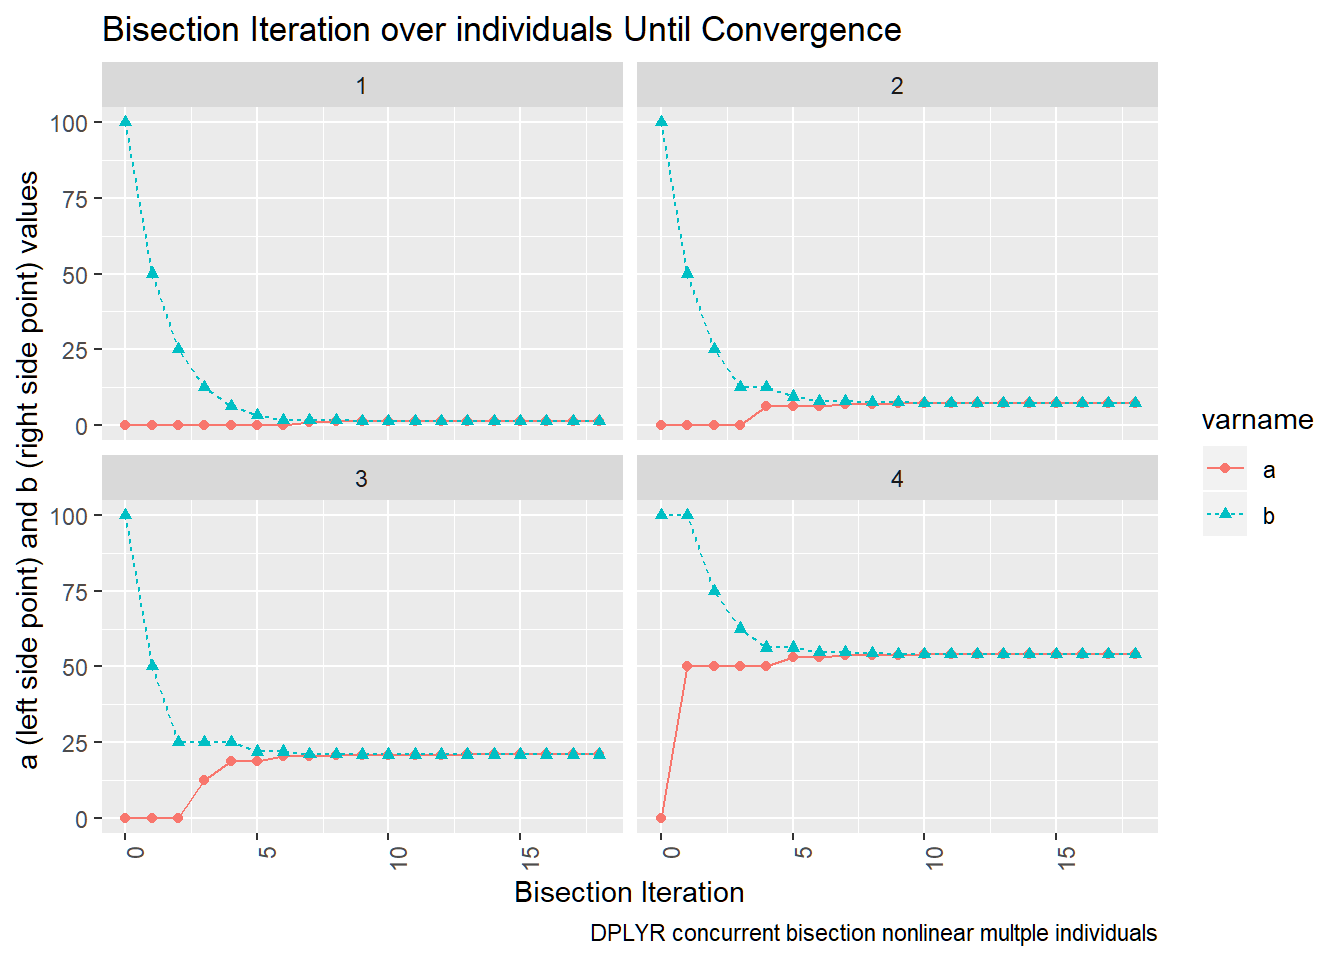
\includegraphics{Panel-Data-and-Optimization-with-R_files/figure-latex/reshape solution for graphing-1} \end{center}

\hypertarget{mathmatics-and-statistics}{%
\chapter{Mathmatics and Statistics}\label{mathmatics-and-statistics}}

\hypertarget{distributions}{%
\section{Distributions}\label{distributions}}

\hypertarget{integrate-over-normal-guassian-process-shock}{%
\subsection{Integrate Over Normal Guassian Process Shock}\label{integrate-over-normal-guassian-process-shock}}

\begin{quote}
Go back to \href{http://fanwangecon.github.io/}{fan}'s \href{https://fanwangecon.github.io/REconTools/}{REconTools} Package, \href{https://fanwangecon.github.io/R4Econ/}{R Code Examples} Repository (\href{https://fanwangecon.github.io/R4Econ/bookdown}{bookdown site}), or \href{https://fanwangecon.github.io/Stat4Econ/}{Intro Stats with R} Repository (\href{https://fanwangecon.github.io/Stat4Econ/bookdown}{bookdown site}).
\end{quote}

Some Common parameters

\begin{Shaded}
\begin{Highlighting}[]
\NormalTok{fl\_eps\_mean }\OtherTok{=} \DecValTok{10}
\NormalTok{fl\_eps\_sd }\OtherTok{=} \DecValTok{50}
\NormalTok{fl\_cdf\_min }\OtherTok{=} \FloatTok{0.000001}
\NormalTok{fl\_cdf\_max }\OtherTok{=} \FloatTok{0.999999}
\NormalTok{ar\_it\_draws }\OtherTok{\textless{}{-}} \FunctionTok{seq}\NormalTok{(}\DecValTok{1}\NormalTok{, }\DecValTok{1000}\NormalTok{)}
\end{Highlighting}
\end{Shaded}

\hypertarget{randomly-sample-and-integrate-monte-carlo-integration}{%
\subsubsection{Randomly Sample and Integrate (Monte Carlo Integration)}\label{randomly-sample-and-integrate-monte-carlo-integration}}

Compare randomly drawn normal shock mean and known mean. How does simulated mean change with draws. Actual integral equals to \(10\), as sample size increases, the sample mean approaches the integration results, but this is expensive, even with ten thousand draws, not very exact.

\begin{Shaded}
\begin{Highlighting}[]
\CommentTok{\# Simulate Draws}
\FunctionTok{set.seed}\NormalTok{(}\DecValTok{123}\NormalTok{)}
\NormalTok{ar\_fl\_means }\OtherTok{\textless{}{-}}
  \FunctionTok{sapply}\NormalTok{(ar\_it\_draws, }\ControlFlowTok{function}\NormalTok{(x)}
    \FunctionTok{return}\NormalTok{(}\FunctionTok{mean}\NormalTok{(}\FunctionTok{rnorm}\NormalTok{(x[}\DecValTok{1}\NormalTok{], }\AttributeTok{mean=}\NormalTok{fl\_eps\_mean, }\AttributeTok{sd=}\NormalTok{fl\_eps\_sd))))}
\NormalTok{ar\_fl\_sd }\OtherTok{\textless{}{-}}
  \FunctionTok{sapply}\NormalTok{(ar\_it\_draws, }\ControlFlowTok{function}\NormalTok{(x)}
    \FunctionTok{return}\NormalTok{(}\FunctionTok{sd}\NormalTok{(}\FunctionTok{rnorm}\NormalTok{(x[}\DecValTok{1}\NormalTok{], }\AttributeTok{mean=}\NormalTok{fl\_eps\_mean, }\AttributeTok{sd=}\NormalTok{fl\_eps\_sd))))}

\NormalTok{mt\_sample\_means }\OtherTok{\textless{}{-}} \FunctionTok{cbind}\NormalTok{(ar\_it\_draws, ar\_fl\_means, ar\_fl\_sd)}
\FunctionTok{colnames}\NormalTok{(mt\_sample\_means) }\OtherTok{\textless{}{-}} \FunctionTok{c}\NormalTok{(}\StringTok{\textquotesingle{}draw\_count\textquotesingle{}}\NormalTok{, }\StringTok{\textquotesingle{}mean\textquotesingle{}}\NormalTok{, }\StringTok{\textquotesingle{}sd\textquotesingle{}}\NormalTok{)}
\NormalTok{tb\_sample\_means }\OtherTok{\textless{}{-}} \FunctionTok{as\_tibble}\NormalTok{(mt\_sample\_means)}

\CommentTok{\# Graph}
\CommentTok{\# x{-}labels}
\NormalTok{x.labels }\OtherTok{\textless{}{-}} \FunctionTok{c}\NormalTok{(}\StringTok{\textquotesingle{}n=1\textquotesingle{}}\NormalTok{, }\StringTok{\textquotesingle{}n=10\textquotesingle{}}\NormalTok{, }\StringTok{\textquotesingle{}n=100\textquotesingle{}}\NormalTok{, }\StringTok{\textquotesingle{}n=1000\textquotesingle{}}\NormalTok{)}
\NormalTok{x.breaks }\OtherTok{\textless{}{-}} \FunctionTok{c}\NormalTok{(}\DecValTok{1}\NormalTok{, }\DecValTok{10}\NormalTok{, }\DecValTok{100}\NormalTok{, }\DecValTok{1000}\NormalTok{)}

\CommentTok{\# Shared Subtitle}
\NormalTok{st\_subtitle }\OtherTok{\textless{}{-}} \FunctionTok{paste0}\NormalTok{(}\StringTok{\textquotesingle{}https://fanwangecon.github.io/\textquotesingle{}}\NormalTok{,}
                      \StringTok{\textquotesingle{}R4Econ/math/integration/htmlpdfr/fs\_integrate\_normal.html\textquotesingle{}}\NormalTok{)}

\CommentTok{\# Shared Labels}
\NormalTok{slb\_title\_shr }\OtherTok{=} \FunctionTok{paste0}\NormalTok{(}\StringTok{\textquotesingle{}as Sample Size Increases}\SpecialCharTok{\textbackslash{}n}\StringTok{\textquotesingle{}}\NormalTok{,}
                       \StringTok{\textquotesingle{}True Mean=\textquotesingle{}}\NormalTok{, fl\_eps\_mean,}\StringTok{\textquotesingle{}, sd=\textquotesingle{}}\NormalTok{,fl\_eps\_sd)}
\NormalTok{slb\_xtitle }\OtherTok{=} \FunctionTok{paste0}\NormalTok{(}\StringTok{\textquotesingle{}Sample Size\textquotesingle{}}\NormalTok{)}

\CommentTok{\# Graph Results{-}{-}Draw}
\NormalTok{plt\_mean }\OtherTok{\textless{}{-}}\NormalTok{ tb\_sample\_means }\SpecialCharTok{\%\textgreater{}\%}
  \FunctionTok{ggplot}\NormalTok{(}\FunctionTok{aes}\NormalTok{(}\AttributeTok{x=}\NormalTok{draw\_count, }\AttributeTok{y=}\NormalTok{mean)) }\SpecialCharTok{+}
  \FunctionTok{geom\_line}\NormalTok{(}\AttributeTok{size=}\FloatTok{0.75}\NormalTok{) }\SpecialCharTok{+}
  \FunctionTok{labs}\NormalTok{(}\AttributeTok{title =} \FunctionTok{paste0}\NormalTok{(}\StringTok{\textquotesingle{}Sample Mean \textquotesingle{}}\NormalTok{, slb\_title\_shr),}
       \AttributeTok{subtitle =}\NormalTok{ st\_subtitle,}
       \AttributeTok{x =}\NormalTok{ slb\_xtitle,}
       \AttributeTok{y =} \StringTok{\textquotesingle{}Sample Mean\textquotesingle{}}\NormalTok{,}
       \AttributeTok{caption =} \StringTok{\textquotesingle{}Mean of Sample Integrates to True Mean\textquotesingle{}}\NormalTok{) }\SpecialCharTok{+}
  \FunctionTok{scale\_x\_continuous}\NormalTok{(}\AttributeTok{trans=}\StringTok{\textquotesingle{}log10\textquotesingle{}}\NormalTok{, }\AttributeTok{labels =}\NormalTok{ x.labels, }\AttributeTok{breaks =}\NormalTok{ x.breaks) }\SpecialCharTok{+}
  \FunctionTok{theme\_bw}\NormalTok{()}
\FunctionTok{print}\NormalTok{(plt\_mean)}
\end{Highlighting}
\end{Shaded}

\begin{center}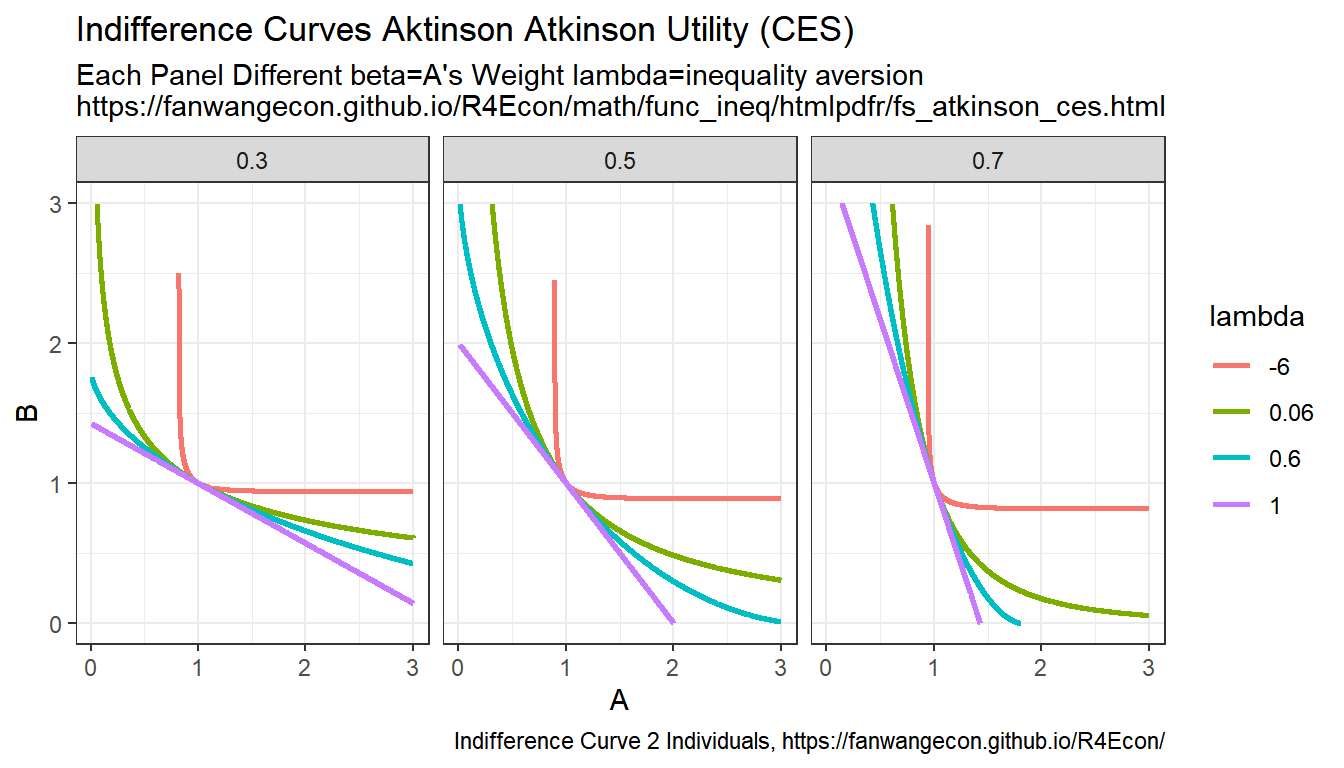
\includegraphics{Panel-Data-and-Optimization-with-R_files/figure-latex/unnamed-chunk-216-1} \end{center}

\begin{Shaded}
\begin{Highlighting}[]
\NormalTok{plt\_sd }\OtherTok{\textless{}{-}}\NormalTok{ tb\_sample\_means }\SpecialCharTok{\%\textgreater{}\%}
  \FunctionTok{ggplot}\NormalTok{(}\FunctionTok{aes}\NormalTok{(}\AttributeTok{x=}\NormalTok{draw\_count, }\AttributeTok{y=}\NormalTok{sd)) }\SpecialCharTok{+}
  \FunctionTok{geom\_line}\NormalTok{(}\AttributeTok{size=}\FloatTok{0.75}\NormalTok{) }\SpecialCharTok{+}
  \FunctionTok{labs}\NormalTok{(}\AttributeTok{title =} \FunctionTok{paste0}\NormalTok{(}\StringTok{\textquotesingle{}Sample Standard Deviation \textquotesingle{}}\NormalTok{, slb\_title\_shr),}
       \AttributeTok{subtitle =}\NormalTok{ st\_subtitle,}
       \AttributeTok{x =}\NormalTok{ slb\_xtitle,}
       \AttributeTok{y =} \StringTok{\textquotesingle{}Sample Standard Deviation\textquotesingle{}}\NormalTok{,}
       \AttributeTok{caption =} \StringTok{\textquotesingle{}Standard Deviation of Sample Integrates to True SD\textquotesingle{}}\NormalTok{) }\SpecialCharTok{+}
  \FunctionTok{scale\_x\_continuous}\NormalTok{(}\AttributeTok{trans=}\StringTok{\textquotesingle{}log10\textquotesingle{}}\NormalTok{, }\AttributeTok{labels =}\NormalTok{ x.labels, }\AttributeTok{breaks =}\NormalTok{ x.breaks) }\SpecialCharTok{+}
  \FunctionTok{theme\_bw}\NormalTok{()}
\FunctionTok{print}\NormalTok{(plt\_sd)}
\end{Highlighting}
\end{Shaded}

\begin{center}\includegraphics{Panel-Data-and-Optimization-with-R_files/figure-latex/unnamed-chunk-216-2} \end{center}

\hypertarget{integration-by-symmetric-uneven-rectangle}{%
\subsubsection{Integration By Symmetric Uneven Rectangle}\label{integration-by-symmetric-uneven-rectangle}}

Draw on even grid from close to 0 to close to 1. Get the corresponding x points to these quantile levels. Distance between x points are not equi-distance but increasing and symmetric away from the mean. Under this approach, each rectangle aims to approximate the same area.

Resulting integration is rectangle based, but rectangle width differ. The rectangles have wider width as they move away from the mean, and thinner width close to the mean. This is much more stable than the random draw method, but note that it converges somewhat slowly to true values as well.

\begin{Shaded}
\begin{Highlighting}[]
\NormalTok{mt\_fl\_means }\OtherTok{\textless{}{-}}
  \FunctionTok{sapply}\NormalTok{(ar\_it\_draws, }\ControlFlowTok{function}\NormalTok{(x) \{}

\NormalTok{    fl\_prob\_break }\OtherTok{=}\NormalTok{ (fl\_cdf\_max }\SpecialCharTok{{-}}\NormalTok{ fl\_cdf\_min)}\SpecialCharTok{/}\NormalTok{(x[}\DecValTok{1}\NormalTok{])}
\NormalTok{    ar\_eps\_bounds }\OtherTok{\textless{}{-}} \FunctionTok{qnorm}\NormalTok{(}\FunctionTok{seq}\NormalTok{(fl\_cdf\_min, fl\_cdf\_max,}
                               \AttributeTok{by=}\NormalTok{(fl\_cdf\_max }\SpecialCharTok{{-}}\NormalTok{ fl\_cdf\_min)}\SpecialCharTok{/}\NormalTok{(x[}\DecValTok{1}\NormalTok{])),}
                           \AttributeTok{mean =}\NormalTok{ fl\_eps\_mean, }\AttributeTok{sd =}\NormalTok{ fl\_eps\_sd)}
\NormalTok{    ar\_eps\_val }\OtherTok{\textless{}{-}}\NormalTok{ (}\FunctionTok{tail}\NormalTok{(ar\_eps\_bounds, }\SpecialCharTok{{-}}\DecValTok{1}\NormalTok{) }\SpecialCharTok{+} \FunctionTok{head}\NormalTok{(ar\_eps\_bounds, }\SpecialCharTok{{-}}\DecValTok{1}\NormalTok{))}\SpecialCharTok{/}\DecValTok{2}
\NormalTok{    ar\_eps\_prb }\OtherTok{\textless{}{-}} \FunctionTok{rep}\NormalTok{(fl\_prob\_break}\SpecialCharTok{/}\NormalTok{(fl\_cdf\_max }\SpecialCharTok{{-}}\NormalTok{ fl\_cdf\_min), x[}\DecValTok{1}\NormalTok{])}
\NormalTok{    ar\_eps\_fev }\OtherTok{\textless{}{-}} \FunctionTok{dnorm}\NormalTok{(ar\_eps\_val,}
                        \AttributeTok{mean =}\NormalTok{ fl\_eps\_mean, }\AttributeTok{sd =}\NormalTok{ fl\_eps\_sd)}

\NormalTok{    fl\_cdf\_total\_approx }\OtherTok{\textless{}{-}} \FunctionTok{sum}\NormalTok{(ar\_eps\_fev}\SpecialCharTok{*}\FunctionTok{diff}\NormalTok{(ar\_eps\_bounds))}
\NormalTok{    fl\_mean\_approx }\OtherTok{\textless{}{-}} \FunctionTok{sum}\NormalTok{(ar\_eps\_val}\SpecialCharTok{*}\NormalTok{(ar\_eps\_fev}\SpecialCharTok{*}\FunctionTok{diff}\NormalTok{(ar\_eps\_bounds)))}
\NormalTok{    fl\_sd\_approx }\OtherTok{\textless{}{-}} \FunctionTok{sqrt}\NormalTok{(}\FunctionTok{sum}\NormalTok{((ar\_eps\_val}\SpecialCharTok{{-}}\NormalTok{fl\_mean\_approx)}\SpecialCharTok{\^{}}\DecValTok{2}\SpecialCharTok{*}\NormalTok{(ar\_eps\_fev}\SpecialCharTok{*}\FunctionTok{diff}\NormalTok{(ar\_eps\_bounds))))}

    \FunctionTok{return}\NormalTok{(}\FunctionTok{list}\NormalTok{(}\AttributeTok{cdf=}\NormalTok{fl\_cdf\_total\_approx, }\AttributeTok{mean=}\NormalTok{fl\_mean\_approx, }\AttributeTok{sd=}\NormalTok{fl\_sd\_approx))}
\NormalTok{  \})}

\NormalTok{mt\_sample\_means }\OtherTok{\textless{}{-}} \FunctionTok{cbind}\NormalTok{(ar\_it\_draws, }\FunctionTok{as\_tibble}\NormalTok{(}\FunctionTok{t}\NormalTok{(mt\_fl\_means)) }\SpecialCharTok{\%\textgreater{}\%} \FunctionTok{unnest}\NormalTok{())}
\FunctionTok{colnames}\NormalTok{(mt\_sample\_means) }\OtherTok{\textless{}{-}} \FunctionTok{c}\NormalTok{(}\StringTok{\textquotesingle{}draw\_count\textquotesingle{}}\NormalTok{, }\StringTok{\textquotesingle{}cdf\textquotesingle{}}\NormalTok{, }\StringTok{\textquotesingle{}mean\textquotesingle{}}\NormalTok{, }\StringTok{\textquotesingle{}sd\textquotesingle{}}\NormalTok{)}
\NormalTok{tb\_sample\_means }\OtherTok{\textless{}{-}} \FunctionTok{as\_tibble}\NormalTok{(mt\_sample\_means)}

\CommentTok{\# Graph}
\CommentTok{\# x{-}labels}
\NormalTok{x.labels }\OtherTok{\textless{}{-}} \FunctionTok{c}\NormalTok{(}\StringTok{\textquotesingle{}n=1\textquotesingle{}}\NormalTok{, }\StringTok{\textquotesingle{}n=10\textquotesingle{}}\NormalTok{, }\StringTok{\textquotesingle{}n=100\textquotesingle{}}\NormalTok{, }\StringTok{\textquotesingle{}n=1000\textquotesingle{}}\NormalTok{)}
\NormalTok{x.breaks }\OtherTok{\textless{}{-}} \FunctionTok{c}\NormalTok{(}\DecValTok{1}\NormalTok{, }\DecValTok{10}\NormalTok{, }\DecValTok{100}\NormalTok{, }\DecValTok{1000}\NormalTok{)}

\CommentTok{\# Shared Labels}
\NormalTok{slb\_title\_shr }\OtherTok{=} \FunctionTok{paste0}\NormalTok{(}\StringTok{\textquotesingle{}as Uneven Rectangle Count Increases}\SpecialCharTok{\textbackslash{}n}\StringTok{\textquotesingle{}}\NormalTok{,}
                       \StringTok{\textquotesingle{}True Mean=\textquotesingle{}}\NormalTok{, fl\_eps\_mean,}\StringTok{\textquotesingle{}, sd=\textquotesingle{}}\NormalTok{,fl\_eps\_sd)}
\NormalTok{slb\_xtitle }\OtherTok{=} \FunctionTok{paste0}\NormalTok{(}\StringTok{\textquotesingle{}Number of Quantile Bins for Uneven Rectangles Approximation\textquotesingle{}}\NormalTok{)}

\CommentTok{\# Graph Results{-}{-}Draw}
\NormalTok{plt\_mean }\OtherTok{\textless{}{-}}\NormalTok{ tb\_sample\_means }\SpecialCharTok{\%\textgreater{}\%}
  \FunctionTok{ggplot}\NormalTok{(}\FunctionTok{aes}\NormalTok{(}\AttributeTok{x=}\NormalTok{draw\_count, }\AttributeTok{y=}\NormalTok{mean)) }\SpecialCharTok{+}
  \FunctionTok{geom\_line}\NormalTok{(}\AttributeTok{size=}\FloatTok{0.75}\NormalTok{) }\SpecialCharTok{+}
  \FunctionTok{labs}\NormalTok{(}\AttributeTok{title =} \FunctionTok{paste0}\NormalTok{(}\StringTok{\textquotesingle{}Average \textquotesingle{}}\NormalTok{, slb\_title\_shr),}
       \AttributeTok{subtitle =}\NormalTok{ st\_subtitle,}
       \AttributeTok{x =}\NormalTok{ slb\_xtitle,}
       \AttributeTok{y =} \StringTok{\textquotesingle{}Approximated Mean\textquotesingle{}}\NormalTok{,}
       \AttributeTok{caption =} \StringTok{\textquotesingle{}Integral Approximation as Uneven Rectangle Count Increases\textquotesingle{}}\NormalTok{) }\SpecialCharTok{+}
  \FunctionTok{scale\_x\_continuous}\NormalTok{(}\AttributeTok{trans=}\StringTok{\textquotesingle{}log10\textquotesingle{}}\NormalTok{, }\AttributeTok{labels =}\NormalTok{ x.labels, }\AttributeTok{breaks =}\NormalTok{ x.breaks) }\SpecialCharTok{+}
  \FunctionTok{theme\_bw}\NormalTok{()}
\FunctionTok{print}\NormalTok{(plt\_mean)}
\end{Highlighting}
\end{Shaded}

\begin{center}\includegraphics{Panel-Data-and-Optimization-with-R_files/figure-latex/unnamed-chunk-217-1} \end{center}

\begin{Shaded}
\begin{Highlighting}[]
\NormalTok{plt\_sd }\OtherTok{\textless{}{-}}\NormalTok{ tb\_sample\_means }\SpecialCharTok{\%\textgreater{}\%}
  \FunctionTok{ggplot}\NormalTok{(}\FunctionTok{aes}\NormalTok{(}\AttributeTok{x=}\NormalTok{draw\_count, }\AttributeTok{y=}\NormalTok{sd)) }\SpecialCharTok{+}
  \FunctionTok{geom\_line}\NormalTok{(}\AttributeTok{size=}\FloatTok{0.75}\NormalTok{) }\SpecialCharTok{+}
  \FunctionTok{labs}\NormalTok{(}\AttributeTok{title =} \FunctionTok{paste0}\NormalTok{(}\StringTok{\textquotesingle{}Standard Deviation \textquotesingle{}}\NormalTok{, slb\_title\_shr),}
       \AttributeTok{subtitle =}\NormalTok{ st\_subtitle,}
       \AttributeTok{x =}\NormalTok{ slb\_xtitle,}
       \AttributeTok{y =} \StringTok{\textquotesingle{}Approximated Standard Deviation\textquotesingle{}}\NormalTok{,}
       \AttributeTok{caption =} \StringTok{\textquotesingle{}Integral Approximation as Uneven Rectangle Count Increases\textquotesingle{}}\NormalTok{) }\SpecialCharTok{+}
  \FunctionTok{scale\_x\_continuous}\NormalTok{(}\AttributeTok{trans=}\StringTok{\textquotesingle{}log10\textquotesingle{}}\NormalTok{, }\AttributeTok{labels =}\NormalTok{ x.labels, }\AttributeTok{breaks =}\NormalTok{ x.breaks) }\SpecialCharTok{+}
  \FunctionTok{theme\_bw}\NormalTok{()}
\FunctionTok{print}\NormalTok{(plt\_sd)}
\end{Highlighting}
\end{Shaded}

\begin{center}\includegraphics{Panel-Data-and-Optimization-with-R_files/figure-latex/unnamed-chunk-217-2} \end{center}

\begin{Shaded}
\begin{Highlighting}[]
\NormalTok{plt\_cdf }\OtherTok{\textless{}{-}}\NormalTok{ tb\_sample\_means }\SpecialCharTok{\%\textgreater{}\%}
  \FunctionTok{ggplot}\NormalTok{(}\FunctionTok{aes}\NormalTok{(}\AttributeTok{x=}\NormalTok{draw\_count, }\AttributeTok{y=}\NormalTok{cdf)) }\SpecialCharTok{+}
  \FunctionTok{geom\_line}\NormalTok{(}\AttributeTok{size=}\FloatTok{0.75}\NormalTok{) }\SpecialCharTok{+}
  \FunctionTok{labs}\NormalTok{(}\AttributeTok{title =} \FunctionTok{paste0}\NormalTok{(}\StringTok{\textquotesingle{}Aggregate Probability \textquotesingle{}}\NormalTok{, slb\_title\_shr),}
       \AttributeTok{subtitle =}\NormalTok{ st\_subtitle,}
       \AttributeTok{x =}\NormalTok{ slb\_xtitle,}
       \AttributeTok{y =} \StringTok{\textquotesingle{}Sum of Uneven Rectangles\textquotesingle{}}\NormalTok{,}
       \AttributeTok{caption =} \StringTok{\textquotesingle{}Sum of Approx. Probability as Uneven Rectangle Count Increases\textquotesingle{}}\NormalTok{) }\SpecialCharTok{+}
  \FunctionTok{scale\_x\_continuous}\NormalTok{(}\AttributeTok{trans=}\StringTok{\textquotesingle{}log10\textquotesingle{}}\NormalTok{, }\AttributeTok{labels =}\NormalTok{ x.labels, }\AttributeTok{breaks =}\NormalTok{ x.breaks) }\SpecialCharTok{+}
  \FunctionTok{theme\_bw}\NormalTok{()}
\FunctionTok{print}\NormalTok{(plt\_cdf)}
\end{Highlighting}
\end{Shaded}

\begin{center}\includegraphics{Panel-Data-and-Optimization-with-R_files/figure-latex/unnamed-chunk-217-3} \end{center}

\hypertarget{integration-by-constant-width-rectangle-trapezoidal-rule}{%
\subsubsection{Integration By Constant Width Rectangle (Trapezoidal rule)}\label{integration-by-constant-width-rectangle-trapezoidal-rule}}

This is implementing even width recentagle, even along x-axix. Rectangle width are the same, height is \(f(x)\). This is even width, but uneven area. Note that this method approximates the true answer much better and more quickly than the prior methods.

\begin{Shaded}
\begin{Highlighting}[]
\NormalTok{mt\_fl\_means }\OtherTok{\textless{}{-}}
  \FunctionTok{sapply}\NormalTok{(ar\_it\_draws, }\ControlFlowTok{function}\NormalTok{(x) \{}

\NormalTok{    fl\_eps\_min }\OtherTok{\textless{}{-}} \FunctionTok{qnorm}\NormalTok{(fl\_cdf\_min, }\AttributeTok{mean =}\NormalTok{ fl\_eps\_mean, }\AttributeTok{sd =}\NormalTok{ fl\_eps\_sd)}
\NormalTok{    fl\_eps\_max }\OtherTok{\textless{}{-}} \FunctionTok{qnorm}\NormalTok{(fl\_cdf\_max, }\AttributeTok{mean =}\NormalTok{ fl\_eps\_mean, }\AttributeTok{sd =}\NormalTok{ fl\_eps\_sd)}
\NormalTok{    fl\_gap }\OtherTok{\textless{}{-}}\NormalTok{ (fl\_eps\_max}\SpecialCharTok{{-}}\NormalTok{fl\_eps\_min)}\SpecialCharTok{/}\NormalTok{(x[}\DecValTok{1}\NormalTok{])}
\NormalTok{    ar\_eps\_bounds }\OtherTok{\textless{}{-}} \FunctionTok{seq}\NormalTok{(fl\_eps\_min, fl\_eps\_max, }\AttributeTok{by=}\NormalTok{fl\_gap)}
\NormalTok{    ar\_eps\_val }\OtherTok{\textless{}{-}}\NormalTok{ (}\FunctionTok{tail}\NormalTok{(ar\_eps\_bounds, }\SpecialCharTok{{-}}\DecValTok{1}\NormalTok{) }\SpecialCharTok{+} \FunctionTok{head}\NormalTok{(ar\_eps\_bounds, }\SpecialCharTok{{-}}\DecValTok{1}\NormalTok{))}\SpecialCharTok{/}\DecValTok{2}
\NormalTok{    ar\_eps\_prb }\OtherTok{\textless{}{-}} \FunctionTok{dnorm}\NormalTok{(ar\_eps\_val, }\AttributeTok{mean =}\NormalTok{ fl\_eps\_mean, }\AttributeTok{sd =}\NormalTok{ fl\_eps\_sd)}\SpecialCharTok{*}\NormalTok{fl\_gap}

\NormalTok{    fl\_cdf\_total\_approx }\OtherTok{\textless{}{-}} \FunctionTok{sum}\NormalTok{(ar\_eps\_prb)}
\NormalTok{    fl\_mean\_approx }\OtherTok{\textless{}{-}} \FunctionTok{sum}\NormalTok{(ar\_eps\_val}\SpecialCharTok{*}\NormalTok{ar\_eps\_prb)}
\NormalTok{    fl\_sd\_approx }\OtherTok{\textless{}{-}} \FunctionTok{sqrt}\NormalTok{(}\FunctionTok{sum}\NormalTok{((ar\_eps\_val}\SpecialCharTok{{-}}\NormalTok{fl\_mean\_approx)}\SpecialCharTok{\^{}}\DecValTok{2}\SpecialCharTok{*}\NormalTok{ar\_eps\_prb))}

    \FunctionTok{return}\NormalTok{(}\FunctionTok{list}\NormalTok{(}\AttributeTok{cdf=}\NormalTok{fl\_cdf\_total\_approx, }\AttributeTok{mean=}\NormalTok{fl\_mean\_approx, }\AttributeTok{sd=}\NormalTok{fl\_sd\_approx))}
\NormalTok{  \})}

\NormalTok{mt\_sample\_means }\OtherTok{\textless{}{-}} \FunctionTok{cbind}\NormalTok{(ar\_it\_draws, }\FunctionTok{as\_tibble}\NormalTok{(}\FunctionTok{t}\NormalTok{(mt\_fl\_means)) }\SpecialCharTok{\%\textgreater{}\%} \FunctionTok{unnest}\NormalTok{())}
\FunctionTok{colnames}\NormalTok{(mt\_sample\_means) }\OtherTok{\textless{}{-}} \FunctionTok{c}\NormalTok{(}\StringTok{\textquotesingle{}draw\_count\textquotesingle{}}\NormalTok{, }\StringTok{\textquotesingle{}cdf\textquotesingle{}}\NormalTok{, }\StringTok{\textquotesingle{}mean\textquotesingle{}}\NormalTok{, }\StringTok{\textquotesingle{}sd\textquotesingle{}}\NormalTok{)}
\NormalTok{tb\_sample\_means }\OtherTok{\textless{}{-}} \FunctionTok{as\_tibble}\NormalTok{(mt\_sample\_means)}

\CommentTok{\# Graph}
\CommentTok{\# x{-}labels}
\NormalTok{x.labels }\OtherTok{\textless{}{-}} \FunctionTok{c}\NormalTok{(}\StringTok{\textquotesingle{}n=1\textquotesingle{}}\NormalTok{, }\StringTok{\textquotesingle{}n=10\textquotesingle{}}\NormalTok{, }\StringTok{\textquotesingle{}n=100\textquotesingle{}}\NormalTok{, }\StringTok{\textquotesingle{}n=1000\textquotesingle{}}\NormalTok{)}
\NormalTok{x.breaks }\OtherTok{\textless{}{-}} \FunctionTok{c}\NormalTok{(}\DecValTok{1}\NormalTok{, }\DecValTok{10}\NormalTok{, }\DecValTok{100}\NormalTok{, }\DecValTok{1000}\NormalTok{)}

\CommentTok{\# Shared Labels}
\NormalTok{slb\_title\_shr }\OtherTok{=} \FunctionTok{paste0}\NormalTok{(}\StringTok{\textquotesingle{}as Even Rectangle Count Increases}\SpecialCharTok{\textbackslash{}n}\StringTok{\textquotesingle{}}\NormalTok{,}
                       \StringTok{\textquotesingle{}True Mean=\textquotesingle{}}\NormalTok{, fl\_eps\_mean,}\StringTok{\textquotesingle{}, sd=\textquotesingle{}}\NormalTok{,fl\_eps\_sd)}
\NormalTok{slb\_xtitle }\OtherTok{=} \FunctionTok{paste0}\NormalTok{(}\StringTok{\textquotesingle{}Number Equi{-}distance Rectangles Bins\textquotesingle{}}\NormalTok{)}

\CommentTok{\# Graph Results{-}{-}Draw}
\NormalTok{plt\_mean }\OtherTok{\textless{}{-}}\NormalTok{ tb\_sample\_means }\SpecialCharTok{\%\textgreater{}\%}
  \FunctionTok{ggplot}\NormalTok{(}\FunctionTok{aes}\NormalTok{(}\AttributeTok{x=}\NormalTok{draw\_count, }\AttributeTok{y=}\NormalTok{mean)) }\SpecialCharTok{+}
  \FunctionTok{geom\_line}\NormalTok{(}\AttributeTok{size=}\FloatTok{0.75}\NormalTok{) }\SpecialCharTok{+}
  \FunctionTok{labs}\NormalTok{(}\AttributeTok{title =} \FunctionTok{paste0}\NormalTok{(}\StringTok{\textquotesingle{}Average \textquotesingle{}}\NormalTok{, slb\_title\_shr),}
       \AttributeTok{subtitle =}\NormalTok{ st\_subtitle,}
       \AttributeTok{x =}\NormalTok{ slb\_xtitle,}
       \AttributeTok{y =} \StringTok{\textquotesingle{}Integrated Mean\textquotesingle{}}\NormalTok{,}
       \AttributeTok{caption =} \StringTok{\textquotesingle{}Integral Approximation as Even Rectangle width decreases\textquotesingle{}}\NormalTok{) }\SpecialCharTok{+}
  \FunctionTok{scale\_x\_continuous}\NormalTok{(}\AttributeTok{trans=}\StringTok{\textquotesingle{}log10\textquotesingle{}}\NormalTok{, }\AttributeTok{labels =}\NormalTok{ x.labels, }\AttributeTok{breaks =}\NormalTok{ x.breaks) }\SpecialCharTok{+}
  \FunctionTok{theme\_bw}\NormalTok{()}
\FunctionTok{print}\NormalTok{(plt\_mean)}
\end{Highlighting}
\end{Shaded}

\begin{center}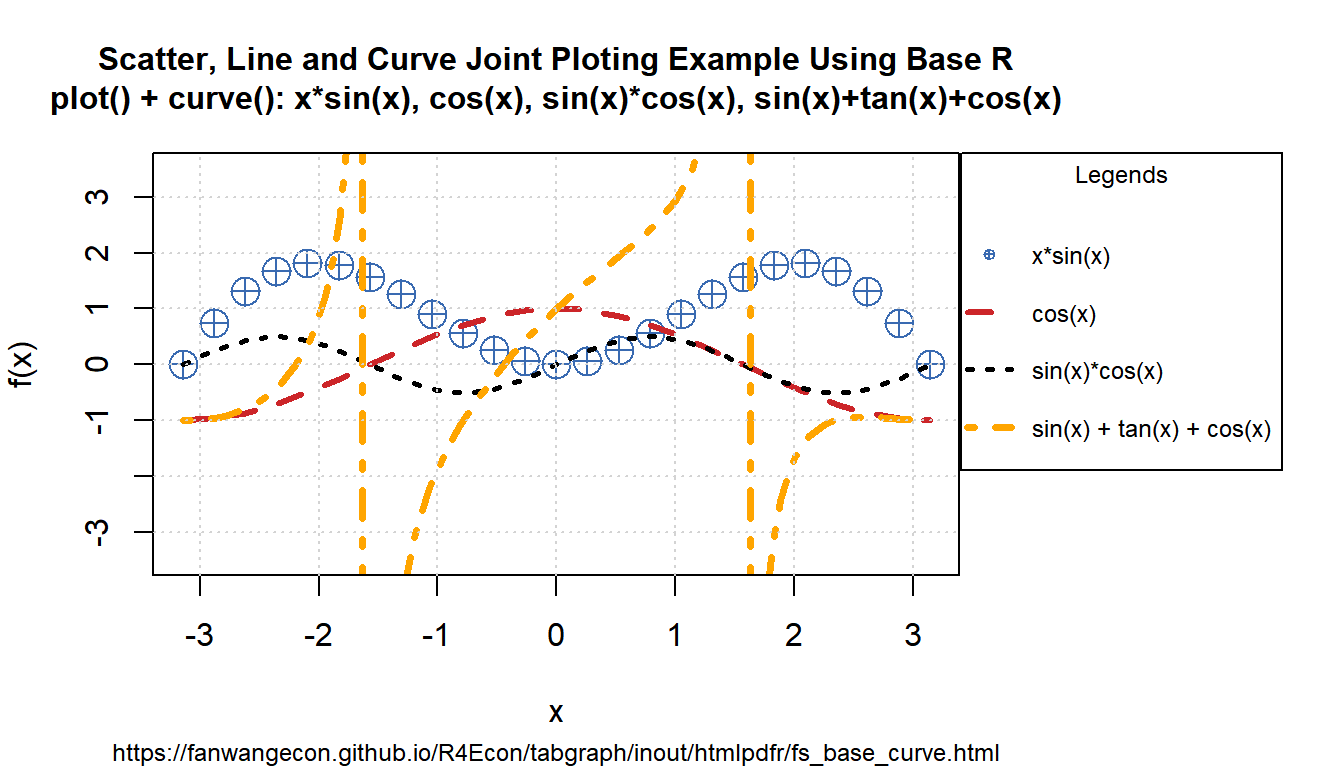
\includegraphics{Panel-Data-and-Optimization-with-R_files/figure-latex/unnamed-chunk-218-1} \end{center}

\begin{Shaded}
\begin{Highlighting}[]
\NormalTok{plt\_sd }\OtherTok{\textless{}{-}}\NormalTok{ tb\_sample\_means }\SpecialCharTok{\%\textgreater{}\%}
  \FunctionTok{ggplot}\NormalTok{(}\FunctionTok{aes}\NormalTok{(}\AttributeTok{x=}\NormalTok{draw\_count, }\AttributeTok{y=}\NormalTok{sd)) }\SpecialCharTok{+}
  \FunctionTok{geom\_line}\NormalTok{(}\AttributeTok{size=}\FloatTok{0.75}\NormalTok{) }\SpecialCharTok{+}
  \FunctionTok{labs}\NormalTok{(}\AttributeTok{title =} \FunctionTok{paste0}\NormalTok{(}\StringTok{\textquotesingle{}Standard Deviation \textquotesingle{}}\NormalTok{, slb\_title\_shr),}
       \AttributeTok{subtitle =}\NormalTok{ st\_subtitle,}
       \AttributeTok{x =}\NormalTok{ slb\_xtitle,}
       \AttributeTok{y =} \StringTok{\textquotesingle{}Standard Deviation\textquotesingle{}}\NormalTok{,}
       \AttributeTok{caption =} \StringTok{\textquotesingle{}Integral Approximation as Even Rectangle width decreases\textquotesingle{}}\NormalTok{) }\SpecialCharTok{+}
  \FunctionTok{scale\_x\_continuous}\NormalTok{(}\AttributeTok{trans=}\StringTok{\textquotesingle{}log10\textquotesingle{}}\NormalTok{, }\AttributeTok{labels =}\NormalTok{ x.labels, }\AttributeTok{breaks =}\NormalTok{ x.breaks) }\SpecialCharTok{+}
  \FunctionTok{theme\_bw}\NormalTok{()}
\FunctionTok{print}\NormalTok{(plt\_sd)}
\end{Highlighting}
\end{Shaded}

\begin{center}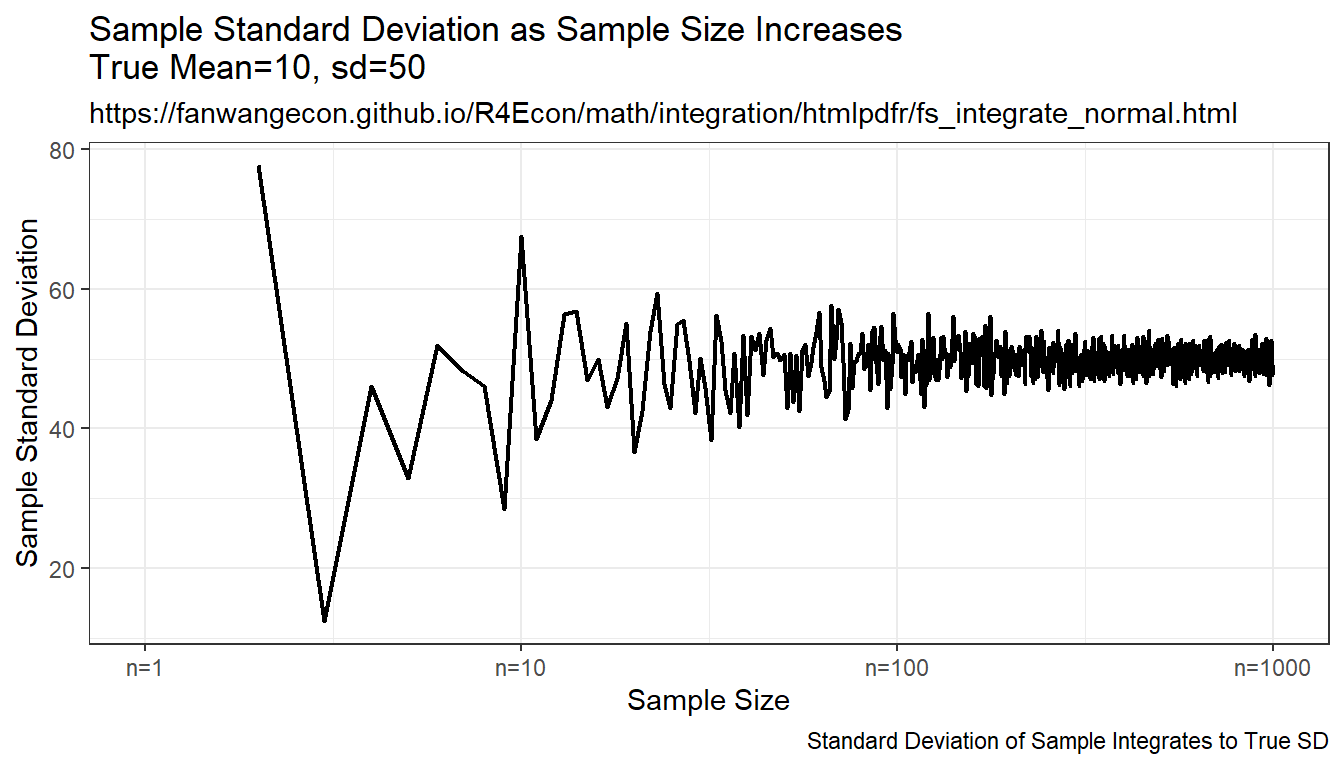
\includegraphics{Panel-Data-and-Optimization-with-R_files/figure-latex/unnamed-chunk-218-2} \end{center}

\begin{Shaded}
\begin{Highlighting}[]
\NormalTok{plt\_cdf }\OtherTok{\textless{}{-}}\NormalTok{ tb\_sample\_means }\SpecialCharTok{\%\textgreater{}\%}
  \FunctionTok{ggplot}\NormalTok{(}\FunctionTok{aes}\NormalTok{(}\AttributeTok{x=}\NormalTok{draw\_count, }\AttributeTok{y=}\NormalTok{cdf)) }\SpecialCharTok{+}
  \FunctionTok{geom\_line}\NormalTok{(}\AttributeTok{size=}\FloatTok{0.75}\NormalTok{) }\SpecialCharTok{+}
  \FunctionTok{labs}\NormalTok{(}\AttributeTok{title =} \FunctionTok{paste0}\NormalTok{(}\StringTok{\textquotesingle{}Aggregate Probability \textquotesingle{}}\NormalTok{, slb\_title\_shr),}
       \AttributeTok{subtitle =}\NormalTok{ st\_subtitle,}
       \AttributeTok{x =}\NormalTok{ slb\_xtitle,}
       \AttributeTok{y =} \StringTok{\textquotesingle{}Sum of Equi{-}Dist Rectangles\textquotesingle{}}\NormalTok{,}
       \AttributeTok{caption =} \StringTok{\textquotesingle{}Sum of Approx. Probability as Equi{-}Dist Rectangle width decreases\textquotesingle{}}\NormalTok{) }\SpecialCharTok{+}
  \FunctionTok{scale\_x\_continuous}\NormalTok{(}\AttributeTok{trans=}\StringTok{\textquotesingle{}log10\textquotesingle{}}\NormalTok{, }\AttributeTok{labels =}\NormalTok{ x.labels, }\AttributeTok{breaks =}\NormalTok{ x.breaks) }\SpecialCharTok{+}
  \FunctionTok{theme\_bw}\NormalTok{()}
\FunctionTok{print}\NormalTok{(plt\_cdf)}
\end{Highlighting}
\end{Shaded}

\begin{center}\includegraphics{Panel-Data-and-Optimization-with-R_files/figure-latex/unnamed-chunk-218-3} \end{center}

\hypertarget{analytical-solutions}{%
\section{Analytical Solutions}\label{analytical-solutions}}

\hypertarget{linear-scalar-fx0-solutions}{%
\subsection{Linear Scalar f(x)=0 Solutions}\label{linear-scalar-fx0-solutions}}

\begin{quote}
Go back to \href{http://fanwangecon.github.io/}{fan}'s \href{https://fanwangecon.github.io/REconTools/}{REconTools} Package, \href{https://fanwangecon.github.io/R4Econ/}{R Code Examples} Repository (\href{https://fanwangecon.github.io/R4Econ/bookdown}{bookdown site}), or \href{https://fanwangecon.github.io/Stat4Econ/}{Intro Stats with R} Repository (\href{https://fanwangecon.github.io/Stat4Econ/bookdown}{bookdown site}).
\end{quote}

\hypertarget{ratio}{%
\subsubsection{Ratio}\label{ratio}}

Here are some common ratios.

\hypertarget{unif-draw-min-and-max-ratio}{%
\paragraph{Unif Draw Min and Max Ratio}\label{unif-draw-min-and-max-ratio}}

We want to draw numbers such that we have some mean \(b\), and that the possible maximum and minimum value drawn are at most \(a\) times apart. Given \(b\) and \(a\), solve for \(x\).

\[
f(x) = \frac{b+x}{b-x} - a = 0
\]

\[
b \cdot a - x \cdot a = b + x \\
b \cdot a - b = x + x \cdot a  \\
b \left(a - 1\right) = x \left( a+ 1\right)  \\
x = \frac{b\left(a-1\right)}{a+1}\\
\]

Uniformly draw

\begin{Shaded}
\begin{Highlighting}[]
\NormalTok{b }\OtherTok{\textless{}{-}} \DecValTok{100}
\NormalTok{a }\OtherTok{\textless{}{-}} \DecValTok{2}
\NormalTok{x }\OtherTok{\textless{}{-}}\NormalTok{ (b}\SpecialCharTok{*}\NormalTok{(a}\DecValTok{{-}1}\NormalTok{))}\SpecialCharTok{/}\NormalTok{(a}\SpecialCharTok{+}\DecValTok{1}\NormalTok{)}
\NormalTok{ar\_unif\_draws }\OtherTok{\textless{}{-}} \FunctionTok{runif}\NormalTok{(}\DecValTok{100}\NormalTok{, }\AttributeTok{min=}\NormalTok{b}\SpecialCharTok{{-}}\NormalTok{x, }\AttributeTok{max=}\NormalTok{b}\SpecialCharTok{+}\NormalTok{x)}
\NormalTok{fl\_max\_min\_ratio }\OtherTok{\textless{}{-}} \FunctionTok{max}\NormalTok{(ar\_unif\_draws)}\SpecialCharTok{/}\FunctionTok{min}\NormalTok{(ar\_unif\_draws)}
\FunctionTok{cat}\NormalTok{(}\StringTok{\textquotesingle{}fl\_max\_min\_ratio =\textquotesingle{}}\NormalTok{, fl\_max\_min\_ratio, }\StringTok{\textquotesingle{}is close to a =\textquotesingle{}}\NormalTok{, a, }\StringTok{\textquotesingle{}}\SpecialCharTok{\textbackslash{}n}\StringTok{\textquotesingle{}}\NormalTok{)}
\end{Highlighting}
\end{Shaded}

\begin{verbatim}
## fl_max_min_ratio = 1.965882 is close to a = 2
\end{verbatim}

\hypertarget{inequality-models}{%
\section{Inequality Models}\label{inequality-models}}

\hypertarget{gini-discrete-sample}{%
\subsection{Gini Discrete Sample}\label{gini-discrete-sample}}

\begin{quote}
Go back to \href{http://fanwangecon.github.io/}{fan}'s \href{https://fanwangecon.github.io/REconTools/}{REconTools} Package, \href{https://fanwangecon.github.io/R4Econ/}{R Code Examples} Repository (\href{https://fanwangecon.github.io/R4Econ/bookdown}{bookdown site}), or \href{https://fanwangecon.github.io/Stat4Econ/}{Intro Stats with R} Repository (\href{https://fanwangecon.github.io/Stat4Econ/bookdown}{bookdown site}).
\end{quote}

This works out how the \href{https://fanwangecon.github.io/REconTools/reference/ff_dist_gini_vector_pos.html}{ff\_dist\_gini\_vector\_pos} function works from \href{https://fanwangecon.github.io/}{Fan}'s \emph{\href{https://fanwangecon.github.io/REconTools/}{REconTools}} Package.

\hypertarget{gini-formula-for-discrete-sample}{%
\subsubsection{Gini Formula for Discrete Sample}\label{gini-formula-for-discrete-sample}}

There is an vector values (all positive). This could be height information for N individuals. It could also be income information for N individuals. Calculate the \href{https://en.wikipedia.org/wiki/Gini_coefficient}{GINI} coefficient treating the given vector as population. This is not an estimation exercise where we want to estimate population gini based on a sample. The given array is the population. The population is discrete, and only has these N individuals in the length n vector.

Note that when the sample size is small, there is a limit to inequality using the formula defined below given each \(N\). So for small \(N\), can not really compare inequality across arrays with different \(N\), can only compare arrays with the same \(N\).

The GINI formula used here is:
\[
 GINI =
  1 - \frac{2}{N+1}
  \cdot
  \left(\sum_{i=1}^N \sum_{j=1}^{i} x_j\right)
  \cdot
  \left(
    \sum_{i=1}^N x_i
  \right)^{-1}
\]

Derive the formula in the steps below.

\emph{Step 1 Area Formula}

\[
 \Gamma = \sum_{i=1}^N \frac{1}{N} \cdot \left(
     \sum_{j=1}^{i} \left(
      \frac{x_j}{\sum_{\widehat{j}=1}^N x_{\widehat{j}} }
      \right)
  \right)
\]

\emph{Step 2 Total Area Given Perfect equality}

With perfect equality \(x_i=a\) for all \(i\), so need to divide by that.

\[
 \Gamma^{\text{equal}} = \sum_{i=1}^N \frac{1}{N} \cdot \left(
     \sum_{j=1}^{i} \left(
      \frac{a}{\sum_{\widehat{j}=1}^N a }
      \right)
  \right)
  = \frac{N+1}{N}\cdot\frac{1}{2}
\]

As the number of elements of the vecotr increases:
\[
 \lim_{N \rightarrow \infty}\Gamma^{\text{equal}}
  = \lim_{N \rightarrow \infty} \frac{N+1}{N}\cdot\frac{1}{2}
  = \frac{1}{2}
\]

\emph{Step 3 Arriving at Finite Vector Gini Formula}

Given what we have from above, we obtain the gini formula, divide by total area below 45 degree line.

\[
 GINI =
  1 -
  \left(\sum_{i=1}^N \sum_{j=1}^{i} x_j\right)
  \cdot
  \left(
    N \cdot \sum_{i=1}^N x_i
  \right)^{-1}
  \cdot
  \left( \frac{N+1}{N}\cdot\frac{1}{2} \right)^{-1}
  =
  1 - \frac{2}{N+1}
  \cdot
  \left(\sum_{i=1}^N \sum_{j=1}^{i} x_j\right)
  \cdot
  \left(
    \sum_{i=1}^N x_i
  \right)^{-1}
\]

\emph{Step 4 Maximum Inequality given N}

Suppose \(x_i=0\) for all \(i<N\), then:

\[
 GINI^{x_i = 0 \text{ except } i=N}
 =
  1 - \frac{2}{N+1}
  \cdot
  X_N
  \cdot
  \left(
    X_N
  \right)^{-1}
 =
 1 - \frac{2}{N+1}
\]

\[
 \lim_{N \rightarrow \infty} GINI^{x_i = 0 \text{ except } i=N}
 =
 1 -
 \lim_{N \rightarrow \infty}
 \frac{2}{N+1}
 = 1
\]

Note that for small N, for example if \(N=10\), even when one person holds all income, all others have 0 income, the formula will not produce gini is zero, but that gini is equal to \(\frac{2}{11}\approx 0.1818\). If \(N=2\), inequality is at most, \(\frac{2}{3}\approx 0.667\).

\[
 MostUnequalGINI\left(N\right) = 1 - \frac{2}{N+1} = \frac{N-1}{N+1}
\]

\hypertarget{implement-gini-formula}{%
\subsubsection{Implement GINI Formula}\label{implement-gini-formula}}

The \textbf{GINI} formula just derived is trivial to compute.

\begin{enumerate}
\def\labelenumi{\arabic{enumi}.}
\tightlist
\item
  scalar: \(\frac{2}{N+1}\)
\item
  cumsum: \(\sum_{j=1}^{i} x_j\)
\item
  sum of cumsum: \(\left(\sum_{i=1}^N \sum_{j=1}^{i} x_j\right)\)
\item
  sum: \(\sum_{i=1}^N X_i\)
\end{enumerate}

There are no package dependencies. Define the formula here:

\begin{Shaded}
\begin{Highlighting}[]
\CommentTok{\# Formula, directly implement the GINI formula Following Step 4 above}
\NormalTok{fv\_dist\_gini\_vector\_pos\_test }\OtherTok{\textless{}{-}} \ControlFlowTok{function}\NormalTok{(ar\_pos) \{}
  \CommentTok{\# Check length and given warning}
\NormalTok{  it\_n }\OtherTok{\textless{}{-}} \FunctionTok{length}\NormalTok{(ar\_pos)}
  \ControlFlowTok{if}\NormalTok{ (it\_n }\SpecialCharTok{\textless{}=} \DecValTok{100}\NormalTok{)  }\FunctionTok{warning}\NormalTok{(}\StringTok{\textquotesingle{}Data vector has n=\textquotesingle{}}\NormalTok{,it\_n,}\StringTok{\textquotesingle{}, max{-}inequality/max{-}gini=\textquotesingle{}}\NormalTok{,(it\_n}\DecValTok{{-}1}\NormalTok{)}\SpecialCharTok{/}\NormalTok{(it\_n }\SpecialCharTok{+} \DecValTok{1}\NormalTok{))}
  \CommentTok{\# Sort}
\NormalTok{  ar\_pos }\OtherTok{\textless{}{-}} \FunctionTok{sort}\NormalTok{(ar\_pos)}
  \CommentTok{\# formula implement}
\NormalTok{  fl\_gini }\OtherTok{\textless{}{-}} \DecValTok{1} \SpecialCharTok{{-}}\NormalTok{ ((}\DecValTok{2}\SpecialCharTok{/}\NormalTok{(it\_n}\SpecialCharTok{+}\DecValTok{1}\NormalTok{)) }\SpecialCharTok{*} \FunctionTok{sum}\NormalTok{(}\FunctionTok{cumsum}\NormalTok{(ar\_pos))}\SpecialCharTok{*}\NormalTok{(}\FunctionTok{sum}\NormalTok{(ar\_pos))}\SpecialCharTok{\^{}}\NormalTok{(}\SpecialCharTok{{-}}\DecValTok{1}\NormalTok{))}
  \FunctionTok{return}\NormalTok{(fl\_gini)}
\NormalTok{\}}
\end{Highlighting}
\end{Shaded}

Generate a number of examples Arrays for testing

\begin{Shaded}
\begin{Highlighting}[]
\CommentTok{\# Example Arrays of data}
\NormalTok{ar\_equal\_n1 }\OtherTok{=} \FunctionTok{c}\NormalTok{(}\DecValTok{1}\NormalTok{)}
\NormalTok{ar\_ineql\_n1 }\OtherTok{=} \FunctionTok{c}\NormalTok{(}\DecValTok{100}\NormalTok{)}

\NormalTok{ar\_equal\_n2 }\OtherTok{=} \FunctionTok{c}\NormalTok{(}\DecValTok{1}\NormalTok{,}\DecValTok{1}\NormalTok{)}
\NormalTok{ar\_ineql\_alittle\_n2 }\OtherTok{=} \FunctionTok{c}\NormalTok{(}\DecValTok{1}\NormalTok{,}\DecValTok{2}\NormalTok{)}
\NormalTok{ar\_ineql\_somewht\_n2 }\OtherTok{=} \FunctionTok{c}\NormalTok{(}\DecValTok{1}\NormalTok{,}\DecValTok{2}\SpecialCharTok{\^{}}\DecValTok{3}\NormalTok{)}
\NormalTok{ar\_ineql\_alotine\_n2 }\OtherTok{=} \FunctionTok{c}\NormalTok{(}\DecValTok{1}\NormalTok{,}\DecValTok{2}\SpecialCharTok{\^{}}\DecValTok{5}\NormalTok{)}
\NormalTok{ar\_ineql\_veryvry\_n2 }\OtherTok{=} \FunctionTok{c}\NormalTok{(}\DecValTok{1}\NormalTok{,}\DecValTok{2}\SpecialCharTok{\^{}}\DecValTok{8}\NormalTok{)}
\NormalTok{ar\_ineql\_mostmst\_n2 }\OtherTok{=} \FunctionTok{c}\NormalTok{(}\DecValTok{1}\NormalTok{,}\DecValTok{2}\SpecialCharTok{\^{}}\DecValTok{13}\NormalTok{)}

\NormalTok{ar\_equal\_n10 }\OtherTok{=} \FunctionTok{c}\NormalTok{(}\DecValTok{2}\NormalTok{,}\DecValTok{2}\NormalTok{,}\DecValTok{2}\NormalTok{,}\DecValTok{2}\NormalTok{,}\DecValTok{2}\NormalTok{,}\DecValTok{2}\NormalTok{, }\DecValTok{2}\NormalTok{, }\DecValTok{2}\NormalTok{, }\DecValTok{2}\NormalTok{, }\DecValTok{2}\NormalTok{)}
\NormalTok{ar\_ineql\_some\_n10 }\OtherTok{=} \FunctionTok{c}\NormalTok{(}\DecValTok{1}\NormalTok{,}\DecValTok{2}\NormalTok{,}\DecValTok{3}\NormalTok{,}\DecValTok{5}\NormalTok{,}\DecValTok{8}\NormalTok{,}\DecValTok{13}\NormalTok{,}\DecValTok{21}\NormalTok{,}\DecValTok{34}\NormalTok{,}\DecValTok{55}\NormalTok{,}\DecValTok{89}\NormalTok{)}
\NormalTok{ar\_ineql\_very\_n10 }\OtherTok{=} \FunctionTok{c}\NormalTok{(}\DecValTok{1}\NormalTok{,}\DecValTok{2}\SpecialCharTok{\^{}}\DecValTok{2}\NormalTok{,}\DecValTok{3}\SpecialCharTok{\^{}}\DecValTok{2}\NormalTok{,}\DecValTok{5}\SpecialCharTok{\^{}}\DecValTok{2}\NormalTok{,}\DecValTok{8}\SpecialCharTok{\^{}}\DecValTok{2}\NormalTok{,}\DecValTok{13}\SpecialCharTok{\^{}}\DecValTok{2}\NormalTok{,}\DecValTok{21}\SpecialCharTok{\^{}}\DecValTok{2}\NormalTok{,}\DecValTok{34}\SpecialCharTok{\^{}}\DecValTok{2}\NormalTok{,}\DecValTok{55}\SpecialCharTok{\^{}}\DecValTok{2}\NormalTok{,}\DecValTok{89}\SpecialCharTok{\^{}}\DecValTok{2}\NormalTok{)}
\NormalTok{ar\_ineql\_extr\_n10 }\OtherTok{=} \FunctionTok{c}\NormalTok{(}\DecValTok{1}\NormalTok{,}\DecValTok{2}\SpecialCharTok{\^{}}\DecValTok{2}\NormalTok{,}\DecValTok{3}\SpecialCharTok{\^{}}\DecValTok{3}\NormalTok{,}\DecValTok{5}\SpecialCharTok{\^{}}\DecValTok{4}\NormalTok{,}\DecValTok{8}\SpecialCharTok{\^{}}\DecValTok{5}\NormalTok{,}\DecValTok{13}\SpecialCharTok{\^{}}\DecValTok{6}\NormalTok{,}\DecValTok{21}\SpecialCharTok{\^{}}\DecValTok{7}\NormalTok{,}\DecValTok{34}\SpecialCharTok{\^{}}\DecValTok{8}\NormalTok{,}\DecValTok{55}\SpecialCharTok{\^{}}\DecValTok{9}\NormalTok{,}\DecValTok{89}\SpecialCharTok{\^{}}\DecValTok{10}\NormalTok{)}
\end{Highlighting}
\end{Shaded}

Now test the example arrays above using the function based no our formula:

\begin{verbatim}
## 
## Small N=1 Hard-Code
\end{verbatim}

\begin{verbatim}
## ar_equal_n1: 0
\end{verbatim}

\begin{verbatim}
## ar_ineql_n1: 0
\end{verbatim}

\begin{verbatim}
## 
## Small N=2 Hard-Code, converge to 1/3, see formula above
\end{verbatim}

\begin{verbatim}
## ar_ineql_alittle_n2: 0.1111111
\end{verbatim}

\begin{verbatim}
## ar_ineql_somewht_n2: 0.2592593
\end{verbatim}

\begin{verbatim}
## ar_ineql_alotine_n2: 0.3131313
\end{verbatim}

\begin{verbatim}
## ar_ineql_veryvry_n2: 0.3307393
\end{verbatim}

\begin{verbatim}
## 
## Small N=10 Hard-Code, convege to 9/11=0.8181, see formula above
\end{verbatim}

\begin{verbatim}
## ar_equal_n10: 0
\end{verbatim}

\begin{verbatim}
## ar_ineql_some_n10: 0.5395514
\end{verbatim}

\begin{verbatim}
## ar_ineql_very_n10: 0.7059554
\end{verbatim}

\begin{verbatim}
## ar_ineql_extr_n10: 0.8181549
\end{verbatim}

\hypertarget{atkinson-inequality-index}{%
\subsection{Atkinson Inequality Index}\label{atkinson-inequality-index}}

\begin{quote}
Go back to \href{http://fanwangecon.github.io/}{fan}'s \href{https://fanwangecon.github.io/REconTools/}{REconTools} Package, \href{https://fanwangecon.github.io/R4Econ/}{R Code Examples} Repository (\href{https://fanwangecon.github.io/R4Econ/bookdown}{bookdown site}), or \href{https://fanwangecon.github.io/Stat4Econ/}{Intro Stats with R} Repository (\href{https://fanwangecon.github.io/Stat4Econ/bookdown}{bookdown site}).
\end{quote}

\hypertarget{atkinson-inequality-measures}{%
\subsubsection{Atkinson Inequality Measures}\label{atkinson-inequality-measures}}

\href{https://linkinghub.elsevier.com/retrieve/pii/0022053170900396}{Atkinson (JET, 1970)} studies five standard inequality measures. Atkinson finds that given the same income data across countries, different inequality measure lead to different rankings of which country is more unequal. Atkinson develops an measure of inequality that changes depending on an inequality aversion parameter.

\[
\text{Atkinson Inequality} =
A\left(
\left\{Y_i\right\}_{i=1}^N,
\lambda
\right)
= 1 -
\left(
\sum_{i=1}^N \frac{1}{N}
  \left(
    \frac{Y_i}{\sum_{j=1}^N \left( \frac{Y_j}{N} \right) }
  \right)^{\lambda}
\right)^{\frac{1}{\lambda}}
\in \left[0,1\right]
\]

\(A\left(\left\{Y_i\right\}_{i=1}^N,\lambda\right)\) equals to zero is perfect equality. 1 is Perfect inequality. If \(\lambda=1\), the inequality measure is always equal to 0 because the planner does not care abouot inequality anymore.

\hypertarget{atkinson-inequality-function}{%
\subsubsection{Atkinson Inequality Function}\label{atkinson-inequality-function}}

Programming up the equation above, we have:

\begin{Shaded}
\begin{Highlighting}[]
\CommentTok{\# Formula}
\NormalTok{ffi\_atkinson\_ineq }\OtherTok{\textless{}{-}} \ControlFlowTok{function}\NormalTok{(ar\_data, fl\_rho) \{}
\NormalTok{  ar\_data\_demean }\OtherTok{\textless{}{-}}\NormalTok{ ar\_data}\SpecialCharTok{/}\FunctionTok{mean}\NormalTok{(ar\_data)}
\NormalTok{  it\_len }\OtherTok{\textless{}{-}} \FunctionTok{length}\NormalTok{(ar\_data\_demean)}
\NormalTok{  fl\_atkinson }\OtherTok{\textless{}{-}} \DecValTok{1} \SpecialCharTok{{-}} \FunctionTok{sum}\NormalTok{(ar\_data\_demean}\SpecialCharTok{\^{}}\NormalTok{\{fl\_rho\}}\SpecialCharTok{*}\NormalTok{(}\DecValTok{1}\SpecialCharTok{/}\NormalTok{it\_len))}\SpecialCharTok{\^{}}\NormalTok{(}\DecValTok{1}\SpecialCharTok{/}\NormalTok{fl\_rho)}
  \FunctionTok{return}\NormalTok{(fl\_atkinson)}
\NormalTok{\}}
\end{Highlighting}
\end{Shaded}

\hypertarget{atkinson-inequality-examples}{%
\subsubsection{Atkinson Inequality Examples}\label{atkinson-inequality-examples}}

Given a vectr of observables, compute the atkinson inequality measure given different inequality aversion.

Preference vector and data vector:

\begin{Shaded}
\begin{Highlighting}[]
\CommentTok{\# Preference Vector}
\NormalTok{ar\_rho }\OtherTok{\textless{}{-}} \FunctionTok{c}\NormalTok{(}\DecValTok{1}\NormalTok{, }\DecValTok{1} \SpecialCharTok{{-}}\NormalTok{ (}\DecValTok{10}\SpecialCharTok{\^{}}\NormalTok{(}\FunctionTok{c}\NormalTok{(}\FunctionTok{seq}\NormalTok{(}\SpecialCharTok{{-}}\FloatTok{2.2}\NormalTok{,}\FloatTok{2.2}\NormalTok{, }\AttributeTok{length.out=}\DecValTok{60}\NormalTok{)))))}
\NormalTok{ar\_rho }\OtherTok{\textless{}{-}} \FunctionTok{unique}\NormalTok{(ar\_rho)}
\NormalTok{mt\_rho }\OtherTok{\textless{}{-}} \FunctionTok{matrix}\NormalTok{(ar\_rho, }\AttributeTok{nrow=}\FunctionTok{length}\NormalTok{(ar\_rho), }\AttributeTok{ncol=}\DecValTok{1}\NormalTok{)}

\CommentTok{\# Random Data Vector (not equal outcomes)}
\FunctionTok{set.seed}\NormalTok{(}\DecValTok{123}\NormalTok{)}
\NormalTok{ar\_data\_rand }\OtherTok{\textless{}{-}} \FunctionTok{rnorm}\NormalTok{(}\DecValTok{15}\NormalTok{, }\AttributeTok{mean=}\DecValTok{0}\NormalTok{,}\AttributeTok{sd=}\DecValTok{1}\NormalTok{)}
\NormalTok{ar\_data\_rand }\OtherTok{\textless{}{-}}\NormalTok{ ar\_data\_rand }\SpecialCharTok{{-}} \FunctionTok{min}\NormalTok{(ar\_data\_rand) }\SpecialCharTok{+} \DecValTok{1}

\CommentTok{\# Uniform Data Vector (Equal)}
\NormalTok{ar\_data\_unif }\OtherTok{\textless{}{-}} \FunctionTok{rep}\NormalTok{(}\DecValTok{1}\NormalTok{, }\FunctionTok{length}\NormalTok{(ar\_data\_rand))}

\CommentTok{\# One Rich (last person has income equal to the sum of all others*100)}
\NormalTok{ar\_data\_onerich }\OtherTok{\textless{}{-}} \FunctionTok{rep}\NormalTok{(}\FloatTok{0.1}\NormalTok{, }\FunctionTok{length}\NormalTok{(ar\_data\_rand))}
\NormalTok{ar\_data\_onerich[}\FunctionTok{length}\NormalTok{(ar\_data\_onerich)] }\OtherTok{=} \FunctionTok{sum}\NormalTok{(}\FunctionTok{head}\NormalTok{(ar\_data\_onerich,}\SpecialCharTok{{-}}\DecValTok{1}\NormalTok{))}\SpecialCharTok{*}\DecValTok{10}
\end{Highlighting}
\end{Shaded}

Testing Atkinson with different data arrays:

\begin{Shaded}
\begin{Highlighting}[]
\CommentTok{\# ATK = 0.1180513}
\FunctionTok{ffi\_atkinson\_ineq}\NormalTok{(ar\_data\_rand, }\SpecialCharTok{{-}}\DecValTok{1}\NormalTok{)}
\end{Highlighting}
\end{Shaded}

\begin{verbatim}
## [1] 0.1180513
\end{verbatim}

\begin{Shaded}
\begin{Highlighting}[]
\CommentTok{\# ATK = 0}
\FunctionTok{ffi\_atkinson\_ineq}\NormalTok{(ar\_data\_unif, }\SpecialCharTok{{-}}\DecValTok{1}\NormalTok{)}
\end{Highlighting}
\end{Shaded}

\begin{verbatim}
## [1] 0
\end{verbatim}

\begin{Shaded}
\begin{Highlighting}[]
\CommentTok{\# ATK = 0.89}
\FunctionTok{ffi\_atkinson\_ineq}\NormalTok{(ar\_data\_onerich, }\SpecialCharTok{{-}}\DecValTok{1}\NormalTok{)}
\end{Highlighting}
\end{Shaded}

\begin{verbatim}
## [1] 0.8956933
\end{verbatim}

\hypertarget{atkinson-inequality-as-inequality-aversion-changes}{%
\paragraph{Atkinson Inequality as Inequality Aversion Changes}\label{atkinson-inequality-as-inequality-aversion-changes}}

This is the vector of inequality aversion parameters:

\begin{Shaded}
\begin{Highlighting}[]
\NormalTok{ar\_rho}
\end{Highlighting}
\end{Shaded}

\begin{verbatim}
##  [1]    1.00000000    0.99369043    0.99250837    0.99110487    0.98943842    0.98745978    0.98511046    0.98232100
##  [9]    0.97900896    0.97507643    0.97040717    0.96486316    0.95828051    0.95046465    0.94118454    0.93016586
## [17]    0.91708291    0.90154895    0.88310482    0.86120530    0.83520306    0.80432947    0.76767192    0.72414684
## [25]    0.67246762    0.61110666    0.53825013    0.45174443    0.34903248    0.22707813    0.08227648   -0.08965279
## [33]   -0.29379184   -0.53617495   -0.82396688   -1.16567469   -1.57139912   -2.05313328   -2.62511705   -3.30425810
## [41]   -4.11063160   -5.06807371   -6.20488608   -7.55467254   -9.15733231  -11.06023949  -13.31964342  -16.00233131
## [49]  -19.18760255  -22.96961271  -27.46015678  -32.79197376  -39.12267043  -46.63938010  -55.56429426  -66.16123043
## [57]  -78.74343059  -93.68282046 -111.42100351 -132.48231461 -157.48931925
\end{verbatim}

How does Atkinson Inequality measure change with respect to a vector of random data as inequality aversion shifts:

\begin{Shaded}
\begin{Highlighting}[]
\FunctionTok{par}\NormalTok{(}\AttributeTok{new=}\NormalTok{T)}
\NormalTok{st\_x\_label }\OtherTok{\textless{}{-}} \StringTok{\textquotesingle{}Lambda, left Rawlsian, right (1) is Utilitarian\textquotesingle{}}
\NormalTok{st\_y\_label }\OtherTok{\textless{}{-}} \StringTok{\textquotesingle{}Atkinson Inequality, 0 = perfect equal\textquotesingle{}}
\NormalTok{ar\_ylim }\OtherTok{=} \FunctionTok{c}\NormalTok{(}\DecValTok{0}\NormalTok{,}\DecValTok{1}\NormalTok{)}
\FunctionTok{ffi\_atkinson\_ineq}\NormalTok{(ar\_data\_rand, }\SpecialCharTok{{-}}\DecValTok{1}\NormalTok{)}
\end{Highlighting}
\end{Shaded}

\begin{verbatim}
## [1] 0.1180513
\end{verbatim}

\begin{Shaded}
\begin{Highlighting}[]
\NormalTok{ar\_atkinson }\OtherTok{\textless{}{-}} \FunctionTok{apply}\NormalTok{(mt\_rho, }\DecValTok{1}\NormalTok{, }\ControlFlowTok{function}\NormalTok{(row)\{}\FunctionTok{ffi\_atkinson\_ineq}\NormalTok{(ar\_data\_rand, row[}\DecValTok{1}\NormalTok{])\})}
\FunctionTok{plot}\NormalTok{(ar\_rho, ar\_atkinson, }\AttributeTok{ylim =}\NormalTok{ ar\_ylim)}
\FunctionTok{title}\NormalTok{(}\AttributeTok{main =} \StringTok{\textquotesingle{}A vector of Random data\textquotesingle{}}\NormalTok{, }\AttributeTok{xlab =}\NormalTok{ st\_x\_label, }\AttributeTok{ylab =}\NormalTok{ st\_y\_label)}
\FunctionTok{grid}\NormalTok{()}
\end{Highlighting}
\end{Shaded}

\begin{center}\includegraphics{Panel-Data-and-Optimization-with-R_files/figure-latex/unnamed-chunk-229-1} \end{center}

Now with the one person has the wealth of all others in the vector times 10:

\begin{Shaded}
\begin{Highlighting}[]
\FunctionTok{par}\NormalTok{(}\AttributeTok{new=}\NormalTok{T)}
\FunctionTok{ffi\_atkinson\_ineq}\NormalTok{(ar\_data\_onerich, }\SpecialCharTok{{-}}\DecValTok{1}\NormalTok{)}
\end{Highlighting}
\end{Shaded}

\begin{verbatim}
## [1] 0.8956933
\end{verbatim}

\begin{Shaded}
\begin{Highlighting}[]
\NormalTok{ar\_atkinson }\OtherTok{\textless{}{-}} \FunctionTok{apply}\NormalTok{(mt\_rho, }\DecValTok{1}\NormalTok{, }\ControlFlowTok{function}\NormalTok{(row)\{}\FunctionTok{ffi\_atkinson\_ineq}\NormalTok{(ar\_data\_onerich, row[}\DecValTok{1}\NormalTok{])\})}
\FunctionTok{plot}\NormalTok{(ar\_rho, ar\_atkinson, }\AttributeTok{ylim =}\NormalTok{ ar\_ylim)}
\FunctionTok{title}\NormalTok{(}\AttributeTok{main =} \StringTok{\textquotesingle{}1 person has the (income of all others summed up)*10\textquotesingle{}}\NormalTok{, }\AttributeTok{xlab =}\NormalTok{ st\_x\_label, }\AttributeTok{ylab =}\NormalTok{ st\_y\_label)}
\FunctionTok{grid}\NormalTok{()}
\end{Highlighting}
\end{Shaded}

\begin{center}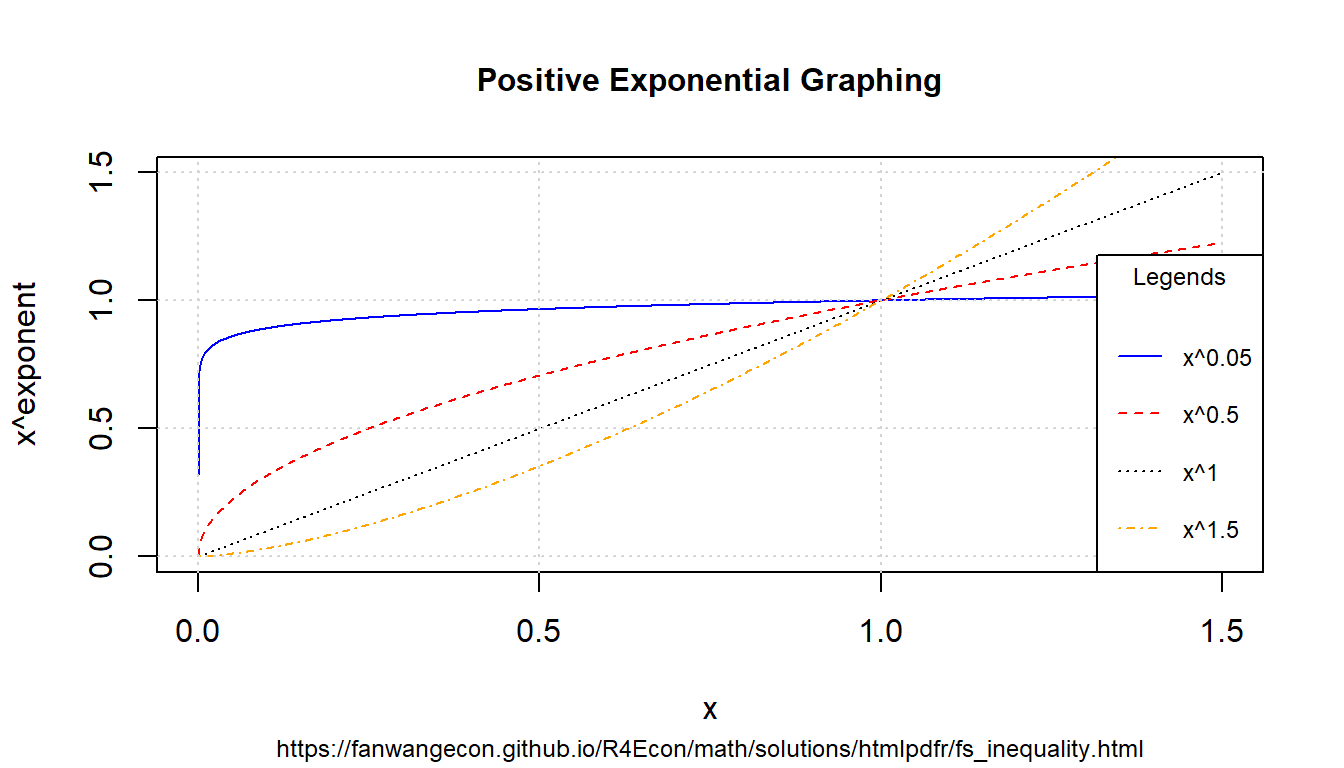
\includegraphics{Panel-Data-and-Optimization-with-R_files/figure-latex/unnamed-chunk-230-1} \end{center}

The Uniform Results, since allocations are uniform, zero for all:

\begin{Shaded}
\begin{Highlighting}[]
\FunctionTok{par}\NormalTok{(}\AttributeTok{new=}\NormalTok{T)}
\FunctionTok{ffi\_atkinson\_ineq}\NormalTok{(ar\_data\_unif, }\SpecialCharTok{{-}}\DecValTok{1}\NormalTok{)}
\end{Highlighting}
\end{Shaded}

\begin{verbatim}
## [1] 0
\end{verbatim}

\begin{Shaded}
\begin{Highlighting}[]
\NormalTok{ar\_atkinson }\OtherTok{\textless{}{-}} \FunctionTok{apply}\NormalTok{(mt\_rho, }\DecValTok{1}\NormalTok{, }\ControlFlowTok{function}\NormalTok{(row)\{}\FunctionTok{ffi\_atkinson\_ineq}\NormalTok{(ar\_data\_unif, row[}\DecValTok{1}\NormalTok{])\})}
\FunctionTok{plot}\NormalTok{(ar\_rho, ar\_atkinson, }\AttributeTok{ylim =}\NormalTok{ ar\_ylim)}
\FunctionTok{title}\NormalTok{(}\AttributeTok{main =} \StringTok{\textquotesingle{}uniform distribution\textquotesingle{}}\NormalTok{, }\AttributeTok{xlab =}\NormalTok{ st\_x\_label, }\AttributeTok{ylab =}\NormalTok{ st\_y\_label)}
\FunctionTok{grid}\NormalTok{()}
\end{Highlighting}
\end{Shaded}

\begin{center}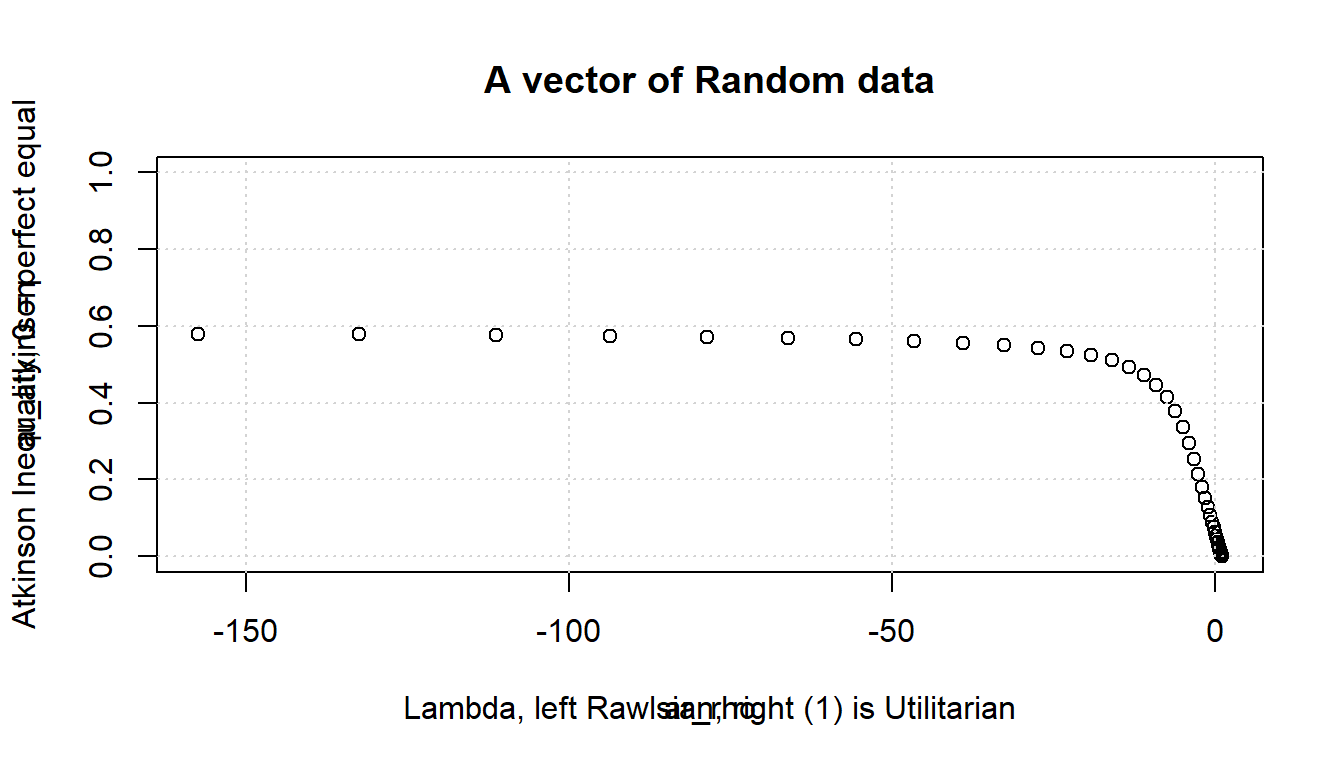
\includegraphics{Panel-Data-and-Optimization-with-R_files/figure-latex/unnamed-chunk-231-1} \end{center}

\hypertarget{analyzing-equation-mechanics}{%
\subsubsection{Analyzing Equation Mechanics}\label{analyzing-equation-mechanics}}

How does the Aktinson Family utility function work? THe Atkinson Family Utility has the following functional form.

\[
V^{\text{social}}
=
\left(
\alpha
\cdot
A^{\lambda}
+
\beta
\cdot
B^{\lambda}
\right)^{\frac{1}{\lambda}}
\]

Several key issues here:

\begin{enumerate}
\def\labelenumi{\arabic{enumi}.}
\tightlist
\item
  \(V^{\text{social}}\) is the utility of some social planner
\item
  \(A\) and \(B\) are allocations for Alex and Ben.
\item
  \(\alpha\) and \(\beta\) are biases that a social planner has for Alex and Ben: \(\alpha+\beta=1\), \(\alpha>0\), and \(\beta>0\)
\item
  \(-\infty < \lambda \le 1\) is a measure of inequality aversion

  \begin{itemize}
  \tightlist
  \item
    \(\lambda=1\) is when the planner cares about weighted total allocations (efficient, Utilitarian)
  \item
    \(\lambda=-\infty\) is when the planner cares about only the minimum between \(A\) and \(B\) allocations (equality, Rawlsian)
  \end{itemize}
\end{enumerate}

What if only care about Alex? Clearly, if the planner only cares about Ben, \(\beta=1\), then:

\[
V^{\text{social}}
=
\left(
B^{\lambda}
\right)^{\frac{1}{\lambda}}
= B
\]

Clearly, regardless of the value of \(\lambda\), as \(B\) increases \(V\) increases. What Happens to V when A or B increases? What is the derivative of \(V\) with respect to \(A\) or \(B\)?

\[
    \frac{\partial V}{\partial A}
    =
    \frac{1}{\lambda}
    \left(
    \alpha
    A^{\lambda}
    +
    \beta
    B^{\lambda}
    \right)^{\frac{1}{\lambda}-1}
    \cdot
    \lambda
    \alpha
    A^{\lambda -1}
\]

\[
    \frac{\partial V}{\partial A}
    =
    \left(
    \alpha
    A^{\lambda}
    +
    \beta
    B^{\lambda}
    \right)^{\frac{1-\lambda}{\lambda}}
    \cdot
    \alpha
    A^{\lambda -1}
    >0
\]

Note that \(\frac{\partial V}{\partial A}>0\). When \(\lambda <0\), \(Z^{\lambda}>0\). For example \(10^{-2}=\frac{1}{100}\). And For example \(0.1^{\frac{3}{-2}}=\frac{1}{0.1^{1.5}}\). Still Positive.

While the overall \(V\) increases with increasing \(A\), but if we did not have the outter power term, the situation is different. In particular, when \(\lambda < 0\):
\[
\text{ if } \lambda <0
\thinspace\thinspace
\text{ then }
\thinspace\thinspace
\frac{d \left(\alpha A^{\lambda} + \beta B^{\lambda}\right)}{dA}=\alpha\lambda A^{\lambda -1}<0
\]
Without the outter \(\frac{1}{\lambda}\) power, negative \(\lambda\) would lead to decreasing weighted sum. But:
\[
\text{ if } \lambda <0
\thinspace\thinspace
\text{ then }
\thinspace\thinspace
\frac{dG^{\frac{1}{\lambda}}}{dG}=\frac{1}{\lambda}\cdot G^{\frac{1-\lambda}{\lambda}}<0
\]
so when \(G\) is increasing and \(\lambda <0\), \(V\) would decrease. But when \(G\left(A,B\right)\) is decreasing, as is the case with increasing \(A\) when \(\lambda <0\), \(V\) will actually increase. This confirms that \(\frac{\partial V}{\partial A}>0\) for \(\lambda <0\). The result is symmetric for \(\lambda >0\).

\hypertarget{indifference-curve-graph}{%
\subsubsection{Indifference Curve Graph}\label{indifference-curve-graph}}

Given \(V^{\ast}\), we can show the combinations of \(A\) and \(B\) points that provide the same utility. We want to be able to potentially draw multiple indifference curves at the same time. Note that indifference curves are defined by \(\alpha\), \(\lambda\) only. Each indifference curve is a set of \(A\) and \(B\) coordinates. So to generate multiple indifference curves means to generate many sets of \(A\), \(B\) associated with different planner preferences, and then these could be graphed out.

\begin{Shaded}
\begin{Highlighting}[]
\CommentTok{\# A as x{-}axis, need bounds on A}
\NormalTok{fl\_A\_min }\OtherTok{=} \FloatTok{0.01}
\NormalTok{fl\_A\_max }\OtherTok{=} \DecValTok{3}
\NormalTok{it\_A\_grid }\OtherTok{=} \DecValTok{10000}

\CommentTok{\# Define parameters}
\CommentTok{\# ar\_lambda \textless{}{-} 1 {-} (10\^{}(c(seq({-}2,2, length.out=3))))}
\NormalTok{ar\_lambda }\OtherTok{\textless{}{-}} \FunctionTok{c}\NormalTok{(}\DecValTok{1}\NormalTok{, }\FloatTok{0.6}\NormalTok{, }\FloatTok{0.06}\NormalTok{, }\SpecialCharTok{{-}}\DecValTok{6}\NormalTok{)}
\NormalTok{ar\_beta }\OtherTok{\textless{}{-}} \FunctionTok{seq}\NormalTok{(}\FloatTok{0.25}\NormalTok{, }\FloatTok{0.75}\NormalTok{, }\AttributeTok{length.out =} \DecValTok{3}\NormalTok{)}
\NormalTok{ar\_beta }\OtherTok{\textless{}{-}} \FunctionTok{c}\NormalTok{(}\FloatTok{0.3}\NormalTok{, }\FloatTok{0.5}\NormalTok{, }\FloatTok{0.7}\NormalTok{)}
\NormalTok{ar\_v\_star }\OtherTok{\textless{}{-}} \FunctionTok{seq}\NormalTok{(}\DecValTok{1}\NormalTok{, }\DecValTok{2}\NormalTok{, }\AttributeTok{length.out =} \DecValTok{1}\NormalTok{)}
\NormalTok{tb\_pref }\OtherTok{\textless{}{-}} \FunctionTok{as\_tibble}\NormalTok{(}\FunctionTok{cbind}\NormalTok{(ar\_lambda)) }\SpecialCharTok{\%\textgreater{}\%}
  \FunctionTok{expand\_grid}\NormalTok{(ar\_beta) }\SpecialCharTok{\%\textgreater{}\%} \FunctionTok{expand\_grid}\NormalTok{(ar\_v\_star) }\SpecialCharTok{\%\textgreater{}\%}
  \FunctionTok{rename\_all}\NormalTok{(}\SpecialCharTok{\textasciitilde{}}\FunctionTok{c}\NormalTok{(}\StringTok{\textquotesingle{}lambda\textquotesingle{}}\NormalTok{, }\StringTok{\textquotesingle{}beta\textquotesingle{}}\NormalTok{, }\StringTok{\textquotesingle{}vstar\textquotesingle{}}\NormalTok{)) }\SpecialCharTok{\%\textgreater{}\%}
  \FunctionTok{rowid\_to\_column}\NormalTok{(}\AttributeTok{var =} \StringTok{"indiff\_id"}\NormalTok{)}

\CommentTok{\# Generate indifference points with apply and anonymous function}
\CommentTok{\# tb\_pref, whatever is selected from it, must be all numeric}
\CommentTok{\# if there are strings, would cause conversion error.}
\NormalTok{ls\_df\_indiff }\OtherTok{\textless{}{-}} \FunctionTok{apply}\NormalTok{(tb\_pref, }\DecValTok{1}\NormalTok{, }\ControlFlowTok{function}\NormalTok{(x)\{}
\NormalTok{  indiff\_id }\OtherTok{\textless{}{-}}\NormalTok{ x[}\DecValTok{1}\NormalTok{]}
\NormalTok{  lambda }\OtherTok{\textless{}{-}}\NormalTok{ x[}\DecValTok{2}\NormalTok{]}
\NormalTok{  beta }\OtherTok{\textless{}{-}}\NormalTok{ x[}\DecValTok{3}\NormalTok{]}
\NormalTok{  vstar }\OtherTok{\textless{}{-}}\NormalTok{ x[}\DecValTok{4}\NormalTok{]}
\NormalTok{  ar\_fl\_A\_indiff }\OtherTok{\textless{}{-}} \FunctionTok{seq}\NormalTok{(fl\_A\_min, fl\_A\_max, }\AttributeTok{length.out=}\NormalTok{it\_A\_grid)}
\NormalTok{  ar\_fl\_B\_indiff }\OtherTok{\textless{}{-}}\NormalTok{ (((vstar}\SpecialCharTok{\^{}}\NormalTok{lambda) }\SpecialCharTok{{-}}
\NormalTok{                        (beta}\SpecialCharTok{*}\NormalTok{ar\_fl\_A\_indiff}\SpecialCharTok{\^{}}\NormalTok{(lambda)))}\SpecialCharTok{/}\NormalTok{(}\DecValTok{1}\SpecialCharTok{{-}}\NormalTok{beta))}\SpecialCharTok{\^{}}\NormalTok{(}\DecValTok{1}\SpecialCharTok{/}\NormalTok{lambda)}
\NormalTok{  mt\_A\_B\_indiff }\OtherTok{\textless{}{-}} \FunctionTok{cbind}\NormalTok{(indiff\_id, lambda, beta, vstar,}
\NormalTok{                         ar\_fl\_A\_indiff, ar\_fl\_B\_indiff)}
  \FunctionTok{colnames}\NormalTok{(mt\_A\_B\_indiff) }\OtherTok{\textless{}{-}} \FunctionTok{c}\NormalTok{(}\StringTok{\textquotesingle{}indiff\_id\textquotesingle{}}\NormalTok{, }\StringTok{\textquotesingle{}lambda\textquotesingle{}}\NormalTok{, }\StringTok{\textquotesingle{}beta\textquotesingle{}}\NormalTok{, }\StringTok{\textquotesingle{}vstar\textquotesingle{}}\NormalTok{,}
                               \StringTok{\textquotesingle{}indiff\_A\textquotesingle{}}\NormalTok{, }\StringTok{\textquotesingle{}indiff\_B\textquotesingle{}}\NormalTok{)}
\NormalTok{  tb\_A\_B\_indiff }\OtherTok{\textless{}{-}} \FunctionTok{as\_tibble}\NormalTok{(mt\_A\_B\_indiff) }\SpecialCharTok{\%\textgreater{}\%}
    \FunctionTok{rowid\_to\_column}\NormalTok{(}\AttributeTok{var =} \StringTok{"A\_grid\_id"}\NormalTok{) }\SpecialCharTok{\%\textgreater{}\%}
    \FunctionTok{filter}\NormalTok{(indiff\_B }\SpecialCharTok{\textgreater{}=} \DecValTok{0} \SpecialCharTok{\&}\NormalTok{ indiff\_B }\SpecialCharTok{\textless{}=} \FunctionTok{max}\NormalTok{(ar\_fl\_A\_indiff))}
  \FunctionTok{return}\NormalTok{(tb\_A\_B\_indiff)}
\NormalTok{\})}
\NormalTok{df\_indiff }\OtherTok{\textless{}{-}} \FunctionTok{do.call}\NormalTok{(rbind, ls\_df\_indiff) }\SpecialCharTok{\%\textgreater{}\%} \FunctionTok{drop\_na}\NormalTok{()}
\end{Highlighting}
\end{Shaded}

Note that many more A grid points are needed to fully plot out the leontief line.

\begin{Shaded}
\begin{Highlighting}[]
\CommentTok{\# Labeling}
\NormalTok{st\_title }\OtherTok{\textless{}{-}} \FunctionTok{paste0}\NormalTok{(}\StringTok{\textquotesingle{}Indifference Curves Aktinson Atkinson Utility (CES)\textquotesingle{}}\NormalTok{)}
\NormalTok{st\_subtitle }\OtherTok{\textless{}{-}} \FunctionTok{paste0}\NormalTok{(}\StringTok{\textquotesingle{}Each Panel Different beta=A}\SpecialCharTok{\textbackslash{}\textquotesingle{}}\StringTok{s Weight lambda=inequality aversion}\SpecialCharTok{\textbackslash{}n}\StringTok{\textquotesingle{}}\NormalTok{,}
                      \StringTok{\textquotesingle{}https://fanwangecon.github.io/\textquotesingle{}}\NormalTok{,}
                      \StringTok{\textquotesingle{}R4Econ/math/func\_ineq/htmlpdfr/fs\_atkinson\_ces.html\textquotesingle{}}\NormalTok{)}
\NormalTok{st\_caption }\OtherTok{\textless{}{-}} \FunctionTok{paste0}\NormalTok{(}\StringTok{\textquotesingle{}Indifference Curve 2 Individuals, \textquotesingle{}}\NormalTok{,}
                     \StringTok{\textquotesingle{}https://fanwangecon.github.io/R4Econ/\textquotesingle{}}\NormalTok{)}
\NormalTok{st\_x\_label }\OtherTok{\textless{}{-}} \StringTok{\textquotesingle{}A\textquotesingle{}}
\NormalTok{st\_y\_label }\OtherTok{\textless{}{-}} \StringTok{\textquotesingle{}B\textquotesingle{}}

\CommentTok{\# Graphing}
\NormalTok{plt\_indiff }\OtherTok{\textless{}{-}}
\NormalTok{  df\_indiff }\SpecialCharTok{\%\textgreater{}\%} \FunctionTok{mutate}\NormalTok{(}\AttributeTok{lambda =} \FunctionTok{as\_factor}\NormalTok{(lambda),}
                       \AttributeTok{beta =} \FunctionTok{as\_factor}\NormalTok{(beta),}
                       \AttributeTok{vstar =} \FunctionTok{as\_factor}\NormalTok{(vstar)) }\SpecialCharTok{\%\textgreater{}\%}
  \FunctionTok{ggplot}\NormalTok{(}\FunctionTok{aes}\NormalTok{(}\AttributeTok{x=}\NormalTok{indiff\_A, }\AttributeTok{y=}\NormalTok{indiff\_B,}
             \AttributeTok{colour=}\NormalTok{lambda)) }\SpecialCharTok{+}
  \FunctionTok{facet\_wrap}\NormalTok{( }\SpecialCharTok{\textasciitilde{}}\NormalTok{ beta) }\SpecialCharTok{+}
  \FunctionTok{geom\_line}\NormalTok{(}\AttributeTok{size=}\DecValTok{1}\NormalTok{) }\SpecialCharTok{+}
  \FunctionTok{labs}\NormalTok{(}\AttributeTok{title =}\NormalTok{ st\_title, }\AttributeTok{subtitle =}\NormalTok{ st\_subtitle,}
       \AttributeTok{x =}\NormalTok{ st\_x\_label, }\AttributeTok{y =}\NormalTok{ st\_y\_label, }\AttributeTok{caption =}\NormalTok{ st\_caption) }\SpecialCharTok{+}
  \FunctionTok{theme\_bw}\NormalTok{()}

\CommentTok{\# show}
\FunctionTok{print}\NormalTok{(plt\_indiff)}
\end{Highlighting}
\end{Shaded}

\begin{center}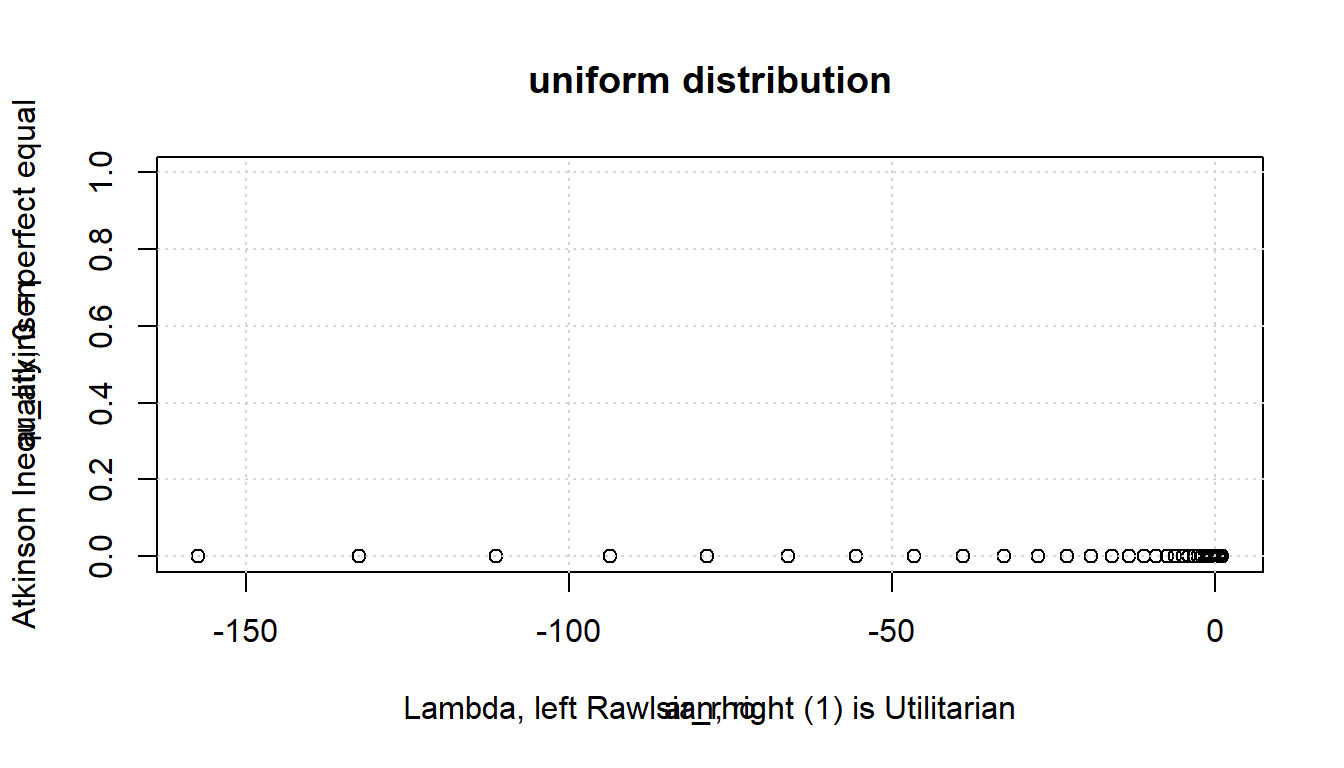
\includegraphics{Panel-Data-and-Optimization-with-R_files/figure-latex/unnamed-chunk-233-1} \end{center}

\hypertarget{location-population-and-pollution}{%
\subsection{Location, Population, and Pollution}\label{location-population-and-pollution}}

\begin{quote}
Go back to \href{http://fanwangecon.github.io/}{fan}'s \href{https://fanwangecon.github.io/REconTools/}{REconTools} Package, \href{https://fanwangecon.github.io/R4Econ/}{R Code Examples} Repository (\href{https://fanwangecon.github.io/R4Econ/bookdown}{bookdown site}), or \href{https://fanwangecon.github.io/Stat4Econ/}{Intro Stats with R} Repository (\href{https://fanwangecon.github.io/Stat4Econ/bookdown}{bookdown site}).
\end{quote}

\hypertarget{simulate-population-distribution-over-location-and-demographics}{%
\subsubsection{Simulate Population Distribution over Location and Demographics}\label{simulate-population-distribution-over-location-and-demographics}}

Use the binomial distribution to generate heterogenous demographic break-down by location. There are N demographic cells, and the binomial distribution provides the probability mass in each of the N cell. Different bernoulli ``win'' chance for each location. There is also probability distribution over population in each location.

First, construct empty population share dataframe:

\begin{Shaded}
\begin{Highlighting}[]
\CommentTok{\# 7 different age groups and 12 different locationso}
\NormalTok{it\_N\_pop\_groups }\OtherTok{\textless{}{-}} \DecValTok{7}
\NormalTok{it\_M\_location }\OtherTok{\textless{}{-}} \DecValTok{12}
\CommentTok{\# Matrix of demographics by location}
\NormalTok{mt\_pop\_data\_frac }\OtherTok{\textless{}{-}} \FunctionTok{matrix}\NormalTok{(}\AttributeTok{data=}\ConstantTok{NA}\NormalTok{, }\AttributeTok{nrow=}\NormalTok{it\_M\_location, }\AttributeTok{ncol=}\NormalTok{it\_N\_pop\_groups)  }
\FunctionTok{colnames}\NormalTok{(mt\_pop\_data\_frac) }\OtherTok{\textless{}{-}} \FunctionTok{paste0}\NormalTok{(}\StringTok{\textquotesingle{}popgrp\textquotesingle{}}\NormalTok{, }\FunctionTok{seq}\NormalTok{(}\DecValTok{1}\NormalTok{,it\_N\_pop\_groups))}
\FunctionTok{rownames}\NormalTok{(mt\_pop\_data\_frac) }\OtherTok{\textless{}{-}} \FunctionTok{paste0}\NormalTok{(}\StringTok{\textquotesingle{}location\textquotesingle{}}\NormalTok{, }\FunctionTok{seq}\NormalTok{(}\DecValTok{1}\NormalTok{,it\_M\_location))}
\CommentTok{\# Display}
\NormalTok{mt\_pop\_data\_frac }\SpecialCharTok{\%\textgreater{}\%} \FunctionTok{kable}\NormalTok{() }\SpecialCharTok{\%\textgreater{}\%} \FunctionTok{kable\_styling\_fc}\NormalTok{()}
\end{Highlighting}
\end{Shaded}

\begin{table}[!h]
\centering
\begin{tabular}{l|l|l|l|l|l|l|l}
\hline
  & popgrp1 & popgrp2 & popgrp3 & popgrp4 & popgrp5 & popgrp6 & popgrp7\\
\hline
\cellcolor{gray!6}{location1} & \cellcolor{gray!6}{NA} & \cellcolor{gray!6}{NA} & \cellcolor{gray!6}{NA} & \cellcolor{gray!6}{NA} & \cellcolor{gray!6}{NA} & \cellcolor{gray!6}{NA} & \cellcolor{gray!6}{NA}\\
\hline
location2 & NA & NA & NA & NA & NA & NA & NA\\
\hline
\cellcolor{gray!6}{location3} & \cellcolor{gray!6}{NA} & \cellcolor{gray!6}{NA} & \cellcolor{gray!6}{NA} & \cellcolor{gray!6}{NA} & \cellcolor{gray!6}{NA} & \cellcolor{gray!6}{NA} & \cellcolor{gray!6}{NA}\\
\hline
location4 & NA & NA & NA & NA & NA & NA & NA\\
\hline
\cellcolor{gray!6}{location5} & \cellcolor{gray!6}{NA} & \cellcolor{gray!6}{NA} & \cellcolor{gray!6}{NA} & \cellcolor{gray!6}{NA} & \cellcolor{gray!6}{NA} & \cellcolor{gray!6}{NA} & \cellcolor{gray!6}{NA}\\
\hline
location6 & NA & NA & NA & NA & NA & NA & NA\\
\hline
\cellcolor{gray!6}{location7} & \cellcolor{gray!6}{NA} & \cellcolor{gray!6}{NA} & \cellcolor{gray!6}{NA} & \cellcolor{gray!6}{NA} & \cellcolor{gray!6}{NA} & \cellcolor{gray!6}{NA} & \cellcolor{gray!6}{NA}\\
\hline
location8 & NA & NA & NA & NA & NA & NA & NA\\
\hline
\cellcolor{gray!6}{location9} & \cellcolor{gray!6}{NA} & \cellcolor{gray!6}{NA} & \cellcolor{gray!6}{NA} & \cellcolor{gray!6}{NA} & \cellcolor{gray!6}{NA} & \cellcolor{gray!6}{NA} & \cellcolor{gray!6}{NA}\\
\hline
location10 & NA & NA & NA & NA & NA & NA & NA\\
\hline
\cellcolor{gray!6}{location11} & \cellcolor{gray!6}{NA} & \cellcolor{gray!6}{NA} & \cellcolor{gray!6}{NA} & \cellcolor{gray!6}{NA} & \cellcolor{gray!6}{NA} & \cellcolor{gray!6}{NA} & \cellcolor{gray!6}{NA}\\
\hline
location12 & NA & NA & NA & NA & NA & NA & NA\\
\hline
\end{tabular}
\end{table}

Second, generate conditional population distribution for each location, and then multiply by the share of population in each locality:

\begin{Shaded}
\begin{Highlighting}[]
\CommentTok{\# Share of population per location}
\FunctionTok{set.seed}\NormalTok{(}\DecValTok{123}\NormalTok{)}
\NormalTok{ar\_p\_loc }\OtherTok{\textless{}{-}} \FunctionTok{dbinom}\NormalTok{(}\DecValTok{0}\SpecialCharTok{:}\NormalTok{(}\DecValTok{3}\SpecialCharTok{*}\NormalTok{it\_M\_location}\DecValTok{{-}1}\NormalTok{), }\DecValTok{3}\SpecialCharTok{*}\NormalTok{it\_M\_location}\DecValTok{{-}1}\NormalTok{, }\FloatTok{0.5}\NormalTok{)}
\NormalTok{it\_start }\OtherTok{\textless{}{-}} \FunctionTok{length}\NormalTok{(ar\_p\_loc)}\SpecialCharTok{/}\DecValTok{2}\SpecialCharTok{{-}}\NormalTok{it\_M\_location}\SpecialCharTok{/}\DecValTok{2}
\NormalTok{ar\_p\_loc }\OtherTok{\textless{}{-}}\NormalTok{ ar\_p\_loc[it\_start}\SpecialCharTok{:}\NormalTok{(it\_start}\SpecialCharTok{+}\NormalTok{it\_M\_location}\SpecialCharTok{+}\DecValTok{1}\NormalTok{)]}
\NormalTok{ar\_p\_loc }\OtherTok{\textless{}{-}}\NormalTok{ ar\_p\_loc}\SpecialCharTok{/}\FunctionTok{sum}\NormalTok{(ar\_p\_loc)}

\CommentTok{\# Different bernoulli "win" probability for each location}
\FunctionTok{set.seed}\NormalTok{(}\DecValTok{234}\NormalTok{)}
\CommentTok{\# ar\_fl\_unif\_prob \textless{}{-} sort(runif(it\_M\_location)*(0.25)+0.4)}
\NormalTok{ar\_fl\_unif\_prob }\OtherTok{\textless{}{-}} \FunctionTok{sort}\NormalTok{(}\FunctionTok{runif}\NormalTok{(it\_M\_location))}

\CommentTok{\# Generate population proportion by locality}
\ControlFlowTok{for}\NormalTok{ (it\_loc }\ControlFlowTok{in} \DecValTok{1}\SpecialCharTok{:}\NormalTok{it\_M\_location ) \{}
\NormalTok{  ar\_p\_pop\_condi\_loc }\OtherTok{\textless{}{-}} \FunctionTok{dbinom}\NormalTok{(}\DecValTok{0}\SpecialCharTok{:}\NormalTok{(it\_N\_pop\_groups}\DecValTok{{-}1}\NormalTok{), it\_N\_pop\_groups}\DecValTok{{-}1}\NormalTok{, ar\_fl\_unif\_prob[it\_loc])}
\NormalTok{  mt\_pop\_data\_frac[it\_loc,] }\OtherTok{\textless{}{-}}\NormalTok{ ar\_p\_pop\_condi\_loc}\SpecialCharTok{*}\NormalTok{ar\_p\_loc[it\_loc]}
\NormalTok{\}}

\CommentTok{\# Sum of cells, should equal to 1}
\FunctionTok{print}\NormalTok{(}\FunctionTok{paste0}\NormalTok{(}\StringTok{\textquotesingle{}pop frac sum = \textquotesingle{}}\NormalTok{, }\FunctionTok{sum}\NormalTok{(mt\_pop\_data\_frac)))}
\end{Highlighting}
\end{Shaded}

\begin{verbatim}
## [1] "pop frac sum = 0.962953679726938"
\end{verbatim}

\begin{Shaded}
\begin{Highlighting}[]
\CommentTok{\# Display}
\FunctionTok{round}\NormalTok{(mt\_pop\_data\_frac}\SpecialCharTok{*}\DecValTok{100}\NormalTok{, }\DecValTok{2}\NormalTok{) }\SpecialCharTok{\%\textgreater{}\%} 
  \FunctionTok{kable}\NormalTok{(}\AttributeTok{caption=}\StringTok{\textquotesingle{}Share of population in each location and demographic cell\textquotesingle{}}\NormalTok{) }\SpecialCharTok{\%\textgreater{}\%} 
  \FunctionTok{kable\_styling\_fc}\NormalTok{()}
\end{Highlighting}
\end{Shaded}

\begin{table}[!h]

\caption{\label{tab:unnamed-chunk-236}Share of population in each location and demographic cell}
\centering
\begin{tabular}[t]{l|r|r|r|r|r|r|r}
\hline
  & popgrp1 & popgrp2 & popgrp3 & popgrp4 & popgrp5 & popgrp6 & popgrp7\\
\hline
\cellcolor{gray!6}{location1} & \cellcolor{gray!6}{1.09} & \cellcolor{gray!6}{0.13} & \cellcolor{gray!6}{0.01} & \cellcolor{gray!6}{0.00} & \cellcolor{gray!6}{0.00} & \cellcolor{gray!6}{0.00} & \cellcolor{gray!6}{0.00}\\
\hline
location2 & 1.63 & 0.70 & 0.13 & 0.01 & 0.00 & 0.00 & 0.00\\
\hline
\cellcolor{gray!6}{location3} & \cellcolor{gray!6}{0.59} & \cellcolor{gray!6}{1.40} & \cellcolor{gray!6}{1.39} & \cellcolor{gray!6}{0.74} & \cellcolor{gray!6}{0.22} & \cellcolor{gray!6}{0.03} & \cellcolor{gray!6}{0.00}\\
\hline
location4 & 0.06 & 0.43 & 1.29 & 2.09 & 1.90 & 0.92 & 0.19\\
\hline
\cellcolor{gray!6}{location5} & \cellcolor{gray!6}{0.07} & \cellcolor{gray!6}{0.55} & \cellcolor{gray!6}{1.73} & \cellcolor{gray!6}{2.89} & \cellcolor{gray!6}{2.71} & \cellcolor{gray!6}{1.36} & \cellcolor{gray!6}{0.28}\\
\hline
location6 & 0.02 & 0.26 & 1.19 & 2.89 & 3.93 & 2.85 & 0.86\\
\hline
\cellcolor{gray!6}{location7} & \cellcolor{gray!6}{0.01} & \cellcolor{gray!6}{0.10} & \cellcolor{gray!6}{0.66} & \cellcolor{gray!6}{2.23} & \cellcolor{gray!6}{4.26} & \cellcolor{gray!6}{4.33} & \cellcolor{gray!6}{1.83}\\
\hline
location8 & 0.00 & 0.06 & 0.47 & 1.83 & 4.03 & 4.72 & 2.31\\
\hline
\cellcolor{gray!6}{location9} & \cellcolor{gray!6}{0.00} & \cellcolor{gray!6}{0.03} & \cellcolor{gray!6}{0.27} & \cellcolor{gray!6}{1.26} & \cellcolor{gray!6}{3.28} & \cellcolor{gray!6}{4.55} & \cellcolor{gray!6}{2.63}\\
\hline
location10 & 0.00 & 0.02 & 0.20 & 0.96 & 2.57 & 3.68 & 2.19\\
\hline
\cellcolor{gray!6}{location11} & \cellcolor{gray!6}{0.00} & \cellcolor{gray!6}{0.00} & \cellcolor{gray!6}{0.00} & \cellcolor{gray!6}{0.04} & \cellcolor{gray!6}{0.40} & \cellcolor{gray!6}{2.05} & \cellcolor{gray!6}{4.38}\\
\hline
location12 & 0.00 & 0.00 & 0.00 & 0.02 & 0.24 & 1.28 & 2.82\\
\hline
\end{tabular}
\end{table}

\hypertarget{simulate-enviromental-exposure}{%
\subsubsection{Simulate Enviromental Exposure}\label{simulate-enviromental-exposure}}

Use log-normal distribution to describe average daily PM10 exposures distribution by locality:

\begin{Shaded}
\begin{Highlighting}[]
\NormalTok{fl\_meanlog }\OtherTok{\textless{}{-}} \FloatTok{3.4}
\NormalTok{fl\_sdlog }\OtherTok{\textless{}{-}} \FloatTok{0.35}
\FunctionTok{hist}\NormalTok{(}\FunctionTok{rlnorm}\NormalTok{(}\DecValTok{1000}\NormalTok{, }\AttributeTok{meanlog =}\NormalTok{ fl\_meanlog, }\AttributeTok{sdlog =}\NormalTok{ fl\_sdlog))}
\end{Highlighting}
\end{Shaded}

\begin{center}\includegraphics{Panel-Data-and-Optimization-with-R_files/figure-latex/unnamed-chunk-237-1} \end{center}

First, draw pollution measure for each locality:

\begin{Shaded}
\begin{Highlighting}[]
\CommentTok{\# draw}
\FunctionTok{set.seed}\NormalTok{(}\DecValTok{123}\NormalTok{)}
\NormalTok{ar\_pollution\_loc }\OtherTok{\textless{}{-}} \FunctionTok{rlnorm}\NormalTok{(it\_M\_location, }\AttributeTok{meanlog =}\NormalTok{ fl\_meanlog, }\AttributeTok{sdlog =}\NormalTok{ fl\_sdlog)}
\CommentTok{\# pollution dataframe}
\CommentTok{\# 5 by 3 matrix}

\CommentTok{\# Column Names}
\NormalTok{ar\_st\_varnames }\OtherTok{\textless{}{-}} \FunctionTok{c}\NormalTok{(}\StringTok{\textquotesingle{}location\textquotesingle{}}\NormalTok{,}\StringTok{\textquotesingle{}avgdailypm10\textquotesingle{}}\NormalTok{)}

\CommentTok{\# Combine to tibble, add name col1, col2, etc.}
\NormalTok{tb\_loc\_pollution }\OtherTok{\textless{}{-}} \FunctionTok{as\_tibble}\NormalTok{(ar\_pollution\_loc) }\SpecialCharTok{\%\textgreater{}\%}
  \FunctionTok{rowid\_to\_column}\NormalTok{(}\AttributeTok{var =} \StringTok{"id"}\NormalTok{) }\SpecialCharTok{\%\textgreater{}\%}
  \FunctionTok{rename\_all}\NormalTok{(}\SpecialCharTok{\textasciitilde{}}\FunctionTok{c}\NormalTok{(ar\_st\_varnames)) }\SpecialCharTok{\%\textgreater{}\%}
  \FunctionTok{mutate}\NormalTok{(}\AttributeTok{location =} \FunctionTok{paste0}\NormalTok{(}\StringTok{\textquotesingle{}location\textquotesingle{}}\NormalTok{, location))}

\CommentTok{\# Display}
\FunctionTok{kable}\NormalTok{(tb\_loc\_pollution) }\SpecialCharTok{\%\textgreater{}\%} \FunctionTok{kable\_styling\_fc}\NormalTok{()}
\end{Highlighting}
\end{Shaded}

\begin{table}[!h]
\centering
\begin{tabular}{l|r}
\hline
location & avgdailypm10\\
\hline
\cellcolor{gray!6}{location1} & \cellcolor{gray!6}{24.62676}\\
\hline
location2 & 27.64481\\
\hline
\cellcolor{gray!6}{location3} & \cellcolor{gray!6}{51.70466}\\
\hline
location4 & 30.71275\\
\hline
\cellcolor{gray!6}{location5} & \cellcolor{gray!6}{31.35114}\\
\hline
location6 & 54.61304\\
\hline
\cellcolor{gray!6}{location7} & \cellcolor{gray!6}{35.20967}\\
\hline
location8 & 19.24456\\
\hline
\cellcolor{gray!6}{location9} & \cellcolor{gray!6}{23.56121}\\
\hline
location10 & 25.63653\\
\hline
\cellcolor{gray!6}{location11} & \cellcolor{gray!6}{45.99021}\\
\hline
location12 & 33.98553\\
\hline
\end{tabular}
\end{table}

Second, reshape population data:

\begin{Shaded}
\begin{Highlighting}[]
\CommentTok{\# Reshape population data, so each observation is location/demo}
\NormalTok{df\_pop\_data\_frac\_long }\OtherTok{\textless{}{-}} \FunctionTok{as\_tibble}\NormalTok{(mt\_pop\_data\_frac, }\AttributeTok{rownames=}\StringTok{\textquotesingle{}location\textquotesingle{}}\NormalTok{) }\SpecialCharTok{\%\textgreater{}\%}
  \FunctionTok{pivot\_longer}\NormalTok{(}\AttributeTok{cols =} \FunctionTok{starts\_with}\NormalTok{(}\StringTok{\textquotesingle{}popgrp\textquotesingle{}}\NormalTok{),}
               \AttributeTok{names\_to =} \FunctionTok{c}\NormalTok{(}\StringTok{\textquotesingle{}popgrp\textquotesingle{}}\NormalTok{),}
               \AttributeTok{names\_pattern =} \FunctionTok{paste0}\NormalTok{(}\StringTok{"popgrp(.*)"}\NormalTok{),}
               \AttributeTok{values\_to =} \StringTok{"pop\_frac"}\NormalTok{)}
\end{Highlighting}
\end{Shaded}

Third, join with pollution data:

\begin{Shaded}
\begin{Highlighting}[]
\CommentTok{\# Reshape population data, so each observation is location/demo}
\NormalTok{df\_pop\_pollution\_long }\OtherTok{\textless{}{-}}\NormalTok{ df\_pop\_data\_frac\_long }\SpecialCharTok{\%\textgreater{}\%}
  \FunctionTok{left\_join}\NormalTok{(tb\_loc\_pollution, }\AttributeTok{by=}\StringTok{\textquotesingle{}location\textquotesingle{}}\NormalTok{)}

\CommentTok{\# display}
\NormalTok{df\_pop\_pollution\_long[}\DecValTok{1}\SpecialCharTok{:}\FunctionTok{round}\NormalTok{(it\_N\_pop\_groups}\SpecialCharTok{*}\FloatTok{2.5}\NormalTok{),] }\SpecialCharTok{\%\textgreater{}\%} \FunctionTok{kable}\NormalTok{() }\SpecialCharTok{\%\textgreater{}\%} \FunctionTok{kable\_styling\_fc}\NormalTok{()}
\end{Highlighting}
\end{Shaded}

\begin{table}[!h]
\centering
\begin{tabular}{l|l|r|r}
\hline
location & popgrp & pop\_frac & avgdailypm10\\
\hline
\cellcolor{gray!6}{location1} & \cellcolor{gray!6}{1} & \cellcolor{gray!6}{0.0109366} & \cellcolor{gray!6}{24.62676}\\
\hline
location1 & 2 & 0.0013417 & 24.62676\\
\hline
\cellcolor{gray!6}{location1} & \cellcolor{gray!6}{3} & \cellcolor{gray!6}{0.0000686} & \cellcolor{gray!6}{24.62676}\\
\hline
location1 & 4 & 0.0000019 & 24.62676\\
\hline
\cellcolor{gray!6}{location1} & \cellcolor{gray!6}{5} & \cellcolor{gray!6}{0.0000000} & \cellcolor{gray!6}{24.62676}\\
\hline
location1 & 6 & 0.0000000 & 24.62676\\
\hline
\cellcolor{gray!6}{location1} & \cellcolor{gray!6}{7} & \cellcolor{gray!6}{0.0000000} & \cellcolor{gray!6}{24.62676}\\
\hline
location2 & 1 & 0.0163003 & 27.64481\\
\hline
\cellcolor{gray!6}{location2} & \cellcolor{gray!6}{2} & \cellcolor{gray!6}{0.0070132} & \cellcolor{gray!6}{27.64481}\\
\hline
location2 & 3 & 0.0012573 & 27.64481\\
\hline
\cellcolor{gray!6}{location2} & \cellcolor{gray!6}{4} & \cellcolor{gray!6}{0.0001202} & \cellcolor{gray!6}{27.64481}\\
\hline
location2 & 5 & 0.0000065 & 27.64481\\
\hline
\cellcolor{gray!6}{location2} & \cellcolor{gray!6}{6} & \cellcolor{gray!6}{0.0000002} & \cellcolor{gray!6}{27.64481}\\
\hline
location2 & 7 & 0.0000000 & 27.64481\\
\hline
\cellcolor{gray!6}{location3} & \cellcolor{gray!6}{1} & \cellcolor{gray!6}{0.0058760} & \cellcolor{gray!6}{51.70466}\\
\hline
location3 & 2 & 0.0140000 & 51.70466\\
\hline
\cellcolor{gray!6}{location3} & \cellcolor{gray!6}{3} & \cellcolor{gray!6}{0.0138984} & \cellcolor{gray!6}{51.70466}\\
\hline
location3 & 4 & 0.0073587 & 51.70466\\
\hline
\end{tabular}
\end{table}

\hypertarget{compute-demographic-group-specific-exposure-distributions}{%
\subsubsection{Compute Demographic Group Specific Exposure Distributions}\label{compute-demographic-group-specific-exposure-distributions}}

What is the p10, median, p90 and mean pollution exposure for each demographic group?

\begin{enumerate}
\def\labelenumi{\arabic{enumi}.}
\tightlist
\item
  group by population group
\item
  sort by pollution exposure within group
\item
  generate population group specific conditional population weights
\item
  generate population CDF for each population group (sorted by pollution)
\end{enumerate}

\begin{Shaded}
\begin{Highlighting}[]
\CommentTok{\# Follow four steps above}
\NormalTok{df\_pop\_pollution\_by\_popgrp\_cdf }\OtherTok{\textless{}{-}}\NormalTok{ df\_pop\_pollution\_long }\SpecialCharTok{\%\textgreater{}\%}
  \FunctionTok{arrange}\NormalTok{(popgrp, avgdailypm10) }\SpecialCharTok{\%\textgreater{}\%}
  \FunctionTok{group\_by}\NormalTok{(popgrp) }\SpecialCharTok{\%\textgreater{}\%}
  \FunctionTok{mutate}\NormalTok{(}\AttributeTok{cdf\_pop\_condi\_popgrp\_sortpm10 =} \FunctionTok{cumsum}\NormalTok{(pop\_frac}\SpecialCharTok{/}\FunctionTok{sum}\NormalTok{(pop\_frac)))}
\CommentTok{\# display}
\NormalTok{df\_pop\_pollution\_by\_popgrp\_cdf[}\DecValTok{1}\SpecialCharTok{:}\FunctionTok{round}\NormalTok{(it\_N\_pop\_groups}\SpecialCharTok{*}\FloatTok{5.5}\NormalTok{),] }\SpecialCharTok{\%\textgreater{}\%} 
  \FunctionTok{kable}\NormalTok{() }\SpecialCharTok{\%\textgreater{}\%} \FunctionTok{kable\_styling\_fc}\NormalTok{()}
\end{Highlighting}
\end{Shaded}

\begin{table}[!h]
\centering
\begin{tabular}{l|l|r|r|r}
\hline
location & popgrp & pop\_frac & avgdailypm10 & cdf\_pop\_condi\_popgrp\_sortpm10\\
\hline
\cellcolor{gray!6}{location8} & \cellcolor{gray!6}{1} & \cellcolor{gray!6}{0.0000364} & \cellcolor{gray!6}{19.24456} & \cellcolor{gray!6}{0.0010453}\\
\hline
location9 & 1 & 0.0000151 & 23.56121 & 0.0014804\\
\hline
\cellcolor{gray!6}{location1} & \cellcolor{gray!6}{1} & \cellcolor{gray!6}{0.0109366} & \cellcolor{gray!6}{24.62676} & \cellcolor{gray!6}{0.3156484}\\
\hline
location10 & 1 & 0.0000104 & 25.63653 & 0.3159471\\
\hline
\cellcolor{gray!6}{location2} & \cellcolor{gray!6}{1} & \cellcolor{gray!6}{0.0163003} & \cellcolor{gray!6}{27.64481} & \cellcolor{gray!6}{0.7841942}\\
\hline
location4 & 1 & 0.0005879 & 30.71275 & 0.8010816\\
\hline
\cellcolor{gray!6}{location5} & \cellcolor{gray!6}{1} & \cellcolor{gray!6}{0.0007392} & \cellcolor{gray!6}{31.35114} & \cellcolor{gray!6}{0.8223166}\\
\hline
location12 & 1 & 0.0000000 & 33.98553 & 0.8223168\\
\hline
\cellcolor{gray!6}{location7} & \cellcolor{gray!6}{1} & \cellcolor{gray!6}{0.0000681} & \cellcolor{gray!6}{35.20967} & \cellcolor{gray!6}{0.8242718}\\
\hline
location11 & 1 & 0.0000000 & 45.99021 & 0.8242721\\
\hline
\cellcolor{gray!6}{location3} & \cellcolor{gray!6}{1} & \cellcolor{gray!6}{0.0058760} & \cellcolor{gray!6}{51.70466} & \cellcolor{gray!6}{0.9930669}\\
\hline
location6 & 1 & 0.0002413 & 54.61304 & 1.0000000\\
\hline
\cellcolor{gray!6}{location8} & \cellcolor{gray!6}{2} & \cellcolor{gray!6}{0.0006400} & \cellcolor{gray!6}{19.24456} & \cellcolor{gray!6}{0.0172871}\\
\hline
location9 & 2 & 0.0003150 & 23.56121 & 0.0257947\\
\hline
\cellcolor{gray!6}{location1} & \cellcolor{gray!6}{2} & \cellcolor{gray!6}{0.0013417} & \cellcolor{gray!6}{24.62676} & \cellcolor{gray!6}{0.0620374}\\
\hline
location10 & 2 & 0.0002235 & 25.63653 & 0.0680736\\
\hline
\cellcolor{gray!6}{location2} & \cellcolor{gray!6}{2} & \cellcolor{gray!6}{0.0070132} & \cellcolor{gray!6}{27.64481} & \cellcolor{gray!6}{0.2575157}\\
\hline
location4 & 2 & 0.0042712 & 30.71275 & 0.3728918\\
\hline
\cellcolor{gray!6}{location5} & \cellcolor{gray!6}{2} & \cellcolor{gray!6}{0.0055479} & \cellcolor{gray!6}{31.35114} & \cellcolor{gray!6}{0.5227547}\\
\hline
location12 & 2 & 0.0000004 & 33.98553 & 0.5227662\\
\hline
\cellcolor{gray!6}{location7} & \cellcolor{gray!6}{2} & \cellcolor{gray!6}{0.0010378} & \cellcolor{gray!6}{35.20967} & \cellcolor{gray!6}{0.5508009}\\
\hline
location11 & 2 & 0.0000008 & 45.99021 & 0.5508213\\
\hline
\cellcolor{gray!6}{location3} & \cellcolor{gray!6}{2} & \cellcolor{gray!6}{0.0140000} & \cellcolor{gray!6}{51.70466} & \cellcolor{gray!6}{0.9289930}\\
\hline
location6 & 2 & 0.0026287 & 54.61304 & 1.0000000\\
\hline
\cellcolor{gray!6}{location8} & \cellcolor{gray!6}{3} & \cellcolor{gray!6}{0.0046896} & \cellcolor{gray!6}{19.24456} & \cellcolor{gray!6}{0.0638166}\\
\hline
location9 & 3 & 0.0027290 & 23.56121 & 0.1009539\\
\hline
\cellcolor{gray!6}{location1} & \cellcolor{gray!6}{3} & \cellcolor{gray!6}{0.0000686} & \cellcolor{gray!6}{24.62676} & \cellcolor{gray!6}{0.1018872}\\
\hline
location10 & 3 & 0.0020006 & 25.63653 & 0.1291118\\
\hline
\cellcolor{gray!6}{location2} & \cellcolor{gray!6}{3} & \cellcolor{gray!6}{0.0012573} & \cellcolor{gray!6}{27.64481} & \cellcolor{gray!6}{0.1462207}\\
\hline
location4 & 3 & 0.0129304 & 30.71275 & 0.3221799\\
\hline
\cellcolor{gray!6}{location5} & \cellcolor{gray!6}{3} & \cellcolor{gray!6}{0.0173492} & \cellcolor{gray!6}{31.35114} & \cellcolor{gray!6}{0.5582709}\\
\hline
location12 & 3 & 0.0000141 & 33.98553 & 0.5584625\\
\hline
\cellcolor{gray!6}{location7} & \cellcolor{gray!6}{3} & \cellcolor{gray!6}{0.0065945} & \cellcolor{gray!6}{35.20967} & \cellcolor{gray!6}{0.6482016}\\
\hline
location11 & 3 & 0.0000242 & 45.99021 & 0.6485305\\
\hline
\cellcolor{gray!6}{location3} & \cellcolor{gray!6}{3} & \cellcolor{gray!6}{0.0138984} & \cellcolor{gray!6}{51.70466} & \cellcolor{gray!6}{0.8376617}\\
\hline
location6 & 3 & 0.0119295 & 54.61304 & 1.0000000\\
\hline
\cellcolor{gray!6}{location8} & \cellcolor{gray!6}{4} & \cellcolor{gray!6}{0.0183277} & \cellcolor{gray!6}{19.24456} & \cellcolor{gray!6}{0.1224562}\\
\hline
location9 & 4 & 0.0126118 & 23.56121 & 0.2067219\\
\hline
\end{tabular}
\end{table}

Measure quantiles of pollution exposures for different population groups:

\begin{enumerate}
\def\labelenumi{\arabic{enumi}.}
\tightlist
\item
  Consider CDF larger than current quantile of interest.
\item
  Slice group-specific CDF that is higher and closest to quantile of interest.
\item
  Merge results for different quantiles together.
\end{enumerate}

\begin{Shaded}
\begin{Highlighting}[]
\CommentTok{\# Generate pollution quantiles by population groups}
\NormalTok{df\_pop\_pollution\_distribution }\OtherTok{\textless{}{-}}\NormalTok{ df\_pop\_pollution\_by\_popgrp\_cdf }\SpecialCharTok{\%\textgreater{}\%} 
  \FunctionTok{mutate}\NormalTok{(}\AttributeTok{pm10\_mean =} \FunctionTok{weighted.mean}\NormalTok{(avgdailypm10, pop\_frac)) }\SpecialCharTok{\%\textgreater{}\%}
  \FunctionTok{filter}\NormalTok{(cdf\_pop\_condi\_popgrp\_sortpm10 }\SpecialCharTok{\textgreater{}=} \FloatTok{0.10}\NormalTok{) }\SpecialCharTok{\%\textgreater{}\%}
  \FunctionTok{slice}\NormalTok{(}\DecValTok{1}\NormalTok{) }\SpecialCharTok{\%\textgreater{}\%}
  \FunctionTok{mutate}\NormalTok{(}\AttributeTok{pm10\_p10 =}\NormalTok{ avgdailypm10) }\SpecialCharTok{\%\textgreater{}\%}
  \FunctionTok{select}\NormalTok{(popgrp, pm10\_mean, pm10\_p10) }\SpecialCharTok{\%\textgreater{}\%}
  \FunctionTok{left\_join}\NormalTok{(df\_pop\_pollution\_by\_popgrp\_cdf }\SpecialCharTok{\%\textgreater{}\%} 
              \FunctionTok{filter}\NormalTok{(cdf\_pop\_condi\_popgrp\_sortpm10 }\SpecialCharTok{\textgreater{}=} \FloatTok{0.20}\NormalTok{) }\SpecialCharTok{\%\textgreater{}\%}
              \FunctionTok{slice}\NormalTok{(}\DecValTok{1}\NormalTok{) }\SpecialCharTok{\%\textgreater{}\%}
              \FunctionTok{mutate}\NormalTok{(}\AttributeTok{pm10\_p20 =}\NormalTok{ avgdailypm10) }\SpecialCharTok{\%\textgreater{}\%}
              \FunctionTok{select}\NormalTok{(popgrp, pm10\_p20), }
            \AttributeTok{by=}\StringTok{\textquotesingle{}popgrp\textquotesingle{}}\NormalTok{) }\SpecialCharTok{\%\textgreater{}\%}
  \FunctionTok{left\_join}\NormalTok{(df\_pop\_pollution\_by\_popgrp\_cdf }\SpecialCharTok{\%\textgreater{}\%} 
              \FunctionTok{filter}\NormalTok{(cdf\_pop\_condi\_popgrp\_sortpm10 }\SpecialCharTok{\textgreater{}=} \FloatTok{0.50}\NormalTok{) }\SpecialCharTok{\%\textgreater{}\%}
              \FunctionTok{slice}\NormalTok{(}\DecValTok{1}\NormalTok{) }\SpecialCharTok{\%\textgreater{}\%}
              \FunctionTok{mutate}\NormalTok{(}\AttributeTok{pm10\_p50 =}\NormalTok{ avgdailypm10) }\SpecialCharTok{\%\textgreater{}\%}
              \FunctionTok{select}\NormalTok{(popgrp, pm10\_p50), }
            \AttributeTok{by=}\StringTok{\textquotesingle{}popgrp\textquotesingle{}}\NormalTok{) }\SpecialCharTok{\%\textgreater{}\%}
  \FunctionTok{left\_join}\NormalTok{(df\_pop\_pollution\_by\_popgrp\_cdf }\SpecialCharTok{\%\textgreater{}\%} 
              \FunctionTok{filter}\NormalTok{(cdf\_pop\_condi\_popgrp\_sortpm10 }\SpecialCharTok{\textgreater{}=} \FloatTok{0.80}\NormalTok{) }\SpecialCharTok{\%\textgreater{}\%}
              \FunctionTok{slice}\NormalTok{(}\DecValTok{1}\NormalTok{) }\SpecialCharTok{\%\textgreater{}\%}
              \FunctionTok{mutate}\NormalTok{(}\AttributeTok{pm10\_p80 =}\NormalTok{ avgdailypm10) }\SpecialCharTok{\%\textgreater{}\%}
              \FunctionTok{select}\NormalTok{(popgrp, pm10\_p80), }
            \AttributeTok{by=}\StringTok{\textquotesingle{}popgrp\textquotesingle{}}\NormalTok{) }\SpecialCharTok{\%\textgreater{}\%}
  \FunctionTok{left\_join}\NormalTok{(df\_pop\_pollution\_by\_popgrp\_cdf }\SpecialCharTok{\%\textgreater{}\%} 
              \FunctionTok{filter}\NormalTok{(cdf\_pop\_condi\_popgrp\_sortpm10 }\SpecialCharTok{\textgreater{}=} \FloatTok{0.90}\NormalTok{) }\SpecialCharTok{\%\textgreater{}\%}
              \FunctionTok{slice}\NormalTok{(}\DecValTok{1}\NormalTok{) }\SpecialCharTok{\%\textgreater{}\%}
              \FunctionTok{mutate}\NormalTok{(}\AttributeTok{pm10\_p90 =}\NormalTok{ avgdailypm10) }\SpecialCharTok{\%\textgreater{}\%}
              \FunctionTok{select}\NormalTok{(popgrp, pm10\_p90), }
            \AttributeTok{by=}\StringTok{\textquotesingle{}popgrp\textquotesingle{}}\NormalTok{)}
\CommentTok{\# display}
\NormalTok{df\_pop\_pollution\_distribution }\SpecialCharTok{\%\textgreater{}\%} 
  \FunctionTok{kable}\NormalTok{(}\AttributeTok{caption =} \StringTok{\textquotesingle{}PM10 Exposure Distribution by Population Groups\textquotesingle{}}\NormalTok{) }\SpecialCharTok{\%\textgreater{}\%} 
  \FunctionTok{kable\_styling\_fc}\NormalTok{()}
\end{Highlighting}
\end{Shaded}

\begin{table}[!h]

\caption{\label{tab:unnamed-chunk-242}PM10 Exposure Distribution by Population Groups}
\centering
\begin{tabular}[t]{l|r|r|r|r|r|r}
\hline
popgrp & pm10\_mean & pm10\_p10 & pm10\_p20 & pm10\_p50 & pm10\_p80 & pm10\_p90\\
\hline
\cellcolor{gray!6}{1} & \cellcolor{gray!6}{31.07894} & \cellcolor{gray!6}{24.62676} & \cellcolor{gray!6}{24.62676} & \cellcolor{gray!6}{27.64481} & \cellcolor{gray!6}{30.71275} & \cellcolor{gray!6}{51.70466}\\
\hline
2 & 39.47897 & 27.64481 & 27.64481 & 31.35114 & 51.70466 & 51.70466\\
\hline
\cellcolor{gray!6}{3} & \cellcolor{gray!6}{37.92901} & \cellcolor{gray!6}{23.56121} & \cellcolor{gray!6}{30.71275} & \cellcolor{gray!6}{31.35114} & \cellcolor{gray!6}{51.70466} & \cellcolor{gray!6}{54.61304}\\
\hline
4 & 34.86470 & 19.24456 & 23.56121 & 31.35114 & 51.70466 & 54.61304\\
\hline
\cellcolor{gray!6}{5} & \cellcolor{gray!6}{32.56731} & \cellcolor{gray!6}{19.24456} & \cellcolor{gray!6}{23.56121} & \cellcolor{gray!6}{30.71275} & \cellcolor{gray!6}{35.20967} & \cellcolor{gray!6}{54.61304}\\
\hline
6 & 31.46626 & 19.24456 & 23.56121 & 25.63653 & 35.20967 & 54.61304\\
\hline
\cellcolor{gray!6}{7} & \cellcolor{gray!6}{33.50541} & \cellcolor{gray!6}{19.24456} & \cellcolor{gray!6}{23.56121} & \cellcolor{gray!6}{33.98553} & \cellcolor{gray!6}{45.99021} & \cellcolor{gray!6}{45.99021}\\
\hline
\end{tabular}
\end{table}

\hypertarget{tables-and-graphs}{%
\chapter{Tables and Graphs}\label{tables-and-graphs}}

\hypertarget{r-base-plots}{%
\section{R Base Plots}\label{r-base-plots}}

\hypertarget{plot-curve-line-and-points}{%
\subsection{Plot Curve, Line and Points}\label{plot-curve-line-and-points}}

\begin{quote}
Go back to \href{http://fanwangecon.github.io/}{fan}'s \href{https://fanwangecon.github.io/REconTools/}{REconTools} Package, \href{https://fanwangecon.github.io/R4Econ/}{R Code Examples} Repository (\href{https://fanwangecon.github.io/R4Econ/bookdown}{bookdown site}), or \href{https://fanwangecon.github.io/Stat4Econ/}{Intro Stats with R} Repository (\href{https://fanwangecon.github.io/Stat4Econ/bookdown}{bookdown site}).
\end{quote}

Work with the R plot function.

\hypertarget{one-point-one-line-and-two-curves}{%
\subsubsection{One Point, One Line and Two Curves}\label{one-point-one-line-and-two-curves}}

\begin{itemize}
\tightlist
\item
  r curve on top of plot
\item
  r plot specify pch lty both scatter and line
\item
  r legend outside
\end{itemize}

Jointly plot:

\begin{itemize}
\tightlist
\item
  1 scatter plot
\item
  1 line plot
\item
  2 function curve plots
\end{itemize}

\begin{Shaded}
\begin{Highlighting}[]
\DocumentationTok{\#\#\#\#\#\#\#\#\#\#\#\#\#\#\#\#\#\#\#\#\#\#\#\#\#\#\#\#\#\#\#\#\#\#\#\#\#\#\#\#\#\#\#\#\#\#\#\#\#\#\#\#\#\#\#}
\CommentTok{\# First, Some common Labels:}
\DocumentationTok{\#\#\#\#\#\#\#\#\#\#\#\#\#\#\#\#\#\#\#\#\#\#\#\#\#\#\#\#\#\#\#\#\#\#\#\#\#\#\#\#\#\#\#\#\#\#\#\#\#\#\#\#\#\#\#}
\CommentTok{\# Labeling}
\NormalTok{st\_title }\OtherTok{\textless{}{-}} \FunctionTok{paste0}\NormalTok{(}\StringTok{\textquotesingle{}Scatter, Line and Curve Joint Ploting Example Using Base R}\SpecialCharTok{\textbackslash{}n}\StringTok{\textquotesingle{}}\NormalTok{,}
                   \StringTok{\textquotesingle{}plot() + curve(): x*sin(x), cos(x), sin(x)*cos(x), sin(x)+tan(x)+cos(x)\textquotesingle{}}\NormalTok{)}
\NormalTok{st\_subtitle }\OtherTok{\textless{}{-}} \FunctionTok{paste0}\NormalTok{(}\StringTok{\textquotesingle{}https://fanwangecon.github.io/\textquotesingle{}}\NormalTok{,}
                      \StringTok{\textquotesingle{}R4Econ/tabgraph/inout/htmlpdfr/fs\_base\_curve.html\textquotesingle{}}\NormalTok{)}
\NormalTok{st\_x\_label }\OtherTok{\textless{}{-}} \StringTok{\textquotesingle{}x\textquotesingle{}}
\NormalTok{st\_y\_label }\OtherTok{\textless{}{-}} \StringTok{\textquotesingle{}f(x)\textquotesingle{}}

\DocumentationTok{\#\#\#\#\#\#\#\#\#\#\#\#\#\#\#\#\#\#\#\#\#\#\#\#\#\#\#\#\#\#\#\#\#\#\#\#\#\#\#\#\#\#\#\#\#\#\#\#\#\#\#\#\#\#\#}
\CommentTok{\# Second, Generate the Graphs Functions and data points:}
\DocumentationTok{\#\#\#\#\#\#\#\#\#\#\#\#\#\#\#\#\#\#\#\#\#\#\#\#\#\#\#\#\#\#\#\#\#\#\#\#\#\#\#\#\#\#\#\#\#\#\#\#\#\#\#\#\#\#\#}
\CommentTok{\# x only used for Point 1 and Line 1}
\NormalTok{x }\OtherTok{\textless{}{-}} \FunctionTok{seq}\NormalTok{(}\SpecialCharTok{{-}}\DecValTok{1}\SpecialCharTok{*}\NormalTok{pi, }\DecValTok{1}\SpecialCharTok{*}\NormalTok{pi, }\AttributeTok{length.out=}\DecValTok{25}\NormalTok{)}
\CommentTok{\# Line (Point) 1: Generate X and Y}
\NormalTok{y1 }\OtherTok{\textless{}{-}}\NormalTok{ x}\SpecialCharTok{*}\FunctionTok{sin}\NormalTok{(x)}
\NormalTok{st\_point\_1\_y\_legend }\OtherTok{\textless{}{-}} \StringTok{\textquotesingle{}x*sin(x)\textquotesingle{}}
\CommentTok{\# Line 2: Line Plot}
\NormalTok{y2 }\OtherTok{\textless{}{-}} \FunctionTok{cos}\NormalTok{(x)}
\NormalTok{st\_line\_2\_y\_legend }\OtherTok{\textless{}{-}} \StringTok{\textquotesingle{}cos(x)\textquotesingle{}}
\CommentTok{\# Line 3: Function}
\NormalTok{fc\_sin\_cos\_diff }\OtherTok{\textless{}{-}} \ControlFlowTok{function}\NormalTok{(x) }\FunctionTok{sin}\NormalTok{(x)}\SpecialCharTok{*}\FunctionTok{cos}\NormalTok{(x)}
\NormalTok{st\_line\_3\_y\_legend }\OtherTok{\textless{}{-}} \StringTok{\textquotesingle{}sin(x)*cos(x)\textquotesingle{}}
\CommentTok{\# Line 4: Function}
\NormalTok{fc\_sin\_cos\_tan }\OtherTok{\textless{}{-}} \ControlFlowTok{function}\NormalTok{(x) }\FunctionTok{sin}\NormalTok{(x) }\SpecialCharTok{+} \FunctionTok{cos}\NormalTok{(x) }\SpecialCharTok{+} \FunctionTok{tan}\NormalTok{(x)}
\NormalTok{st\_line\_4\_y\_legend }\OtherTok{\textless{}{-}} \StringTok{\textquotesingle{}sin(x) + tan(x) + cos(x)\textquotesingle{}}

\DocumentationTok{\#\#\#\#\#\#\#\#\#\#\#\#\#\#\#\#\#\#\#\#\#\#\#\#\#\#\#\#\#\#\#\#\#\#\#\#\#\#\#\#\#\#\#\#\#\#\#\#\#\#\#\#\#\#\#}
\CommentTok{\# Third, set:}
\CommentTok{\# {-} point shape and size: *pch* and *cex*}
\CommentTok{\# {-} line type and width: *lty* and *lwd*}
\DocumentationTok{\#\#\#\#\#\#\#\#\#\#\#\#\#\#\#\#\#\#\#\#\#\#\#\#\#\#\#\#\#\#\#\#\#\#\#\#\#\#\#\#\#\#\#\#\#\#\#\#\#\#\#\#\#\#\#}
\CommentTok{\# http://www.sthda.com/english/wiki/r{-}plot{-}pch{-}symbols{-}the{-}different{-}point{-}shapes{-}available{-}in{-}r}
\CommentTok{\# http://www.sthda.com/english/wiki/line{-}types{-}in{-}r{-}lty}
\CommentTok{\# for colors, see: https://fanwangecon.github.io/M4Econ/graph/tools/fs\_color.html}
\NormalTok{st\_point\_1\_blue }\OtherTok{\textless{}{-}} \FunctionTok{rgb}\NormalTok{(}\DecValTok{57}\SpecialCharTok{/}\DecValTok{255}\NormalTok{,}\DecValTok{106}\SpecialCharTok{/}\DecValTok{255}\NormalTok{,}\DecValTok{177}\SpecialCharTok{/}\DecValTok{255}\NormalTok{)}
\NormalTok{st\_line\_2\_red }\OtherTok{\textless{}{-}} \FunctionTok{rgb}\NormalTok{(}\DecValTok{204}\SpecialCharTok{/}\DecValTok{255}\NormalTok{, }\DecValTok{37}\SpecialCharTok{/}\DecValTok{255}\NormalTok{, }\DecValTok{41}\SpecialCharTok{/}\DecValTok{255}\NormalTok{,)}
\NormalTok{st\_line\_3\_black }\OtherTok{\textless{}{-}} \StringTok{\textquotesingle{}black\textquotesingle{}}
\NormalTok{st\_line\_4\_purple }\OtherTok{\textless{}{-}} \StringTok{\textquotesingle{}orange\textquotesingle{}}

\CommentTok{\# point type}
\NormalTok{st\_point\_1\_pch }\OtherTok{\textless{}{-}} \DecValTok{10}
\CommentTok{\# point size}
\NormalTok{st\_point\_1\_cex }\OtherTok{\textless{}{-}} \DecValTok{2}

\CommentTok{\# line type}
\NormalTok{st\_line\_2\_lty }\OtherTok{\textless{}{-}} \StringTok{\textquotesingle{}dashed\textquotesingle{}}
\NormalTok{st\_line\_3\_lty }\OtherTok{\textless{}{-}} \StringTok{\textquotesingle{}dotted\textquotesingle{}}
\NormalTok{st\_line\_4\_lty }\OtherTok{\textless{}{-}} \StringTok{\textquotesingle{}dotdash\textquotesingle{}}
\CommentTok{\# line width}
\NormalTok{st\_line\_2\_lwd }\OtherTok{\textless{}{-}} \DecValTok{3}
\NormalTok{st\_line\_3\_lwd }\OtherTok{\textless{}{-}} \FloatTok{2.5}
\NormalTok{st\_line\_4\_lwd }\OtherTok{\textless{}{-}} \FloatTok{3.5}

\DocumentationTok{\#\#\#\#\#\#\#\#\#\#\#\#\#\#\#\#\#\#\#\#\#\#\#\#\#\#\#\#\#\#\#\#\#\#\#\#\#\#\#\#\#\#\#\#\#\#\#\#\#\#\#\#\#\#\#}
\CommentTok{\# Fourth: Share xlim and ylim}
\DocumentationTok{\#\#\#\#\#\#\#\#\#\#\#\#\#\#\#\#\#\#\#\#\#\#\#\#\#\#\#\#\#\#\#\#\#\#\#\#\#\#\#\#\#\#\#\#\#\#\#\#\#\#\#\#\#\#\#}
\NormalTok{ar\_xlim }\OtherTok{=} \FunctionTok{c}\NormalTok{(}\FunctionTok{min}\NormalTok{(x), }\FunctionTok{max}\NormalTok{(x))}
\NormalTok{ar\_ylim }\OtherTok{=} \FunctionTok{c}\NormalTok{(}\SpecialCharTok{{-}}\FloatTok{3.5}\NormalTok{, }\FloatTok{3.5}\NormalTok{)}

\DocumentationTok{\#\#\#\#\#\#\#\#\#\#\#\#\#\#\#\#\#\#\#\#\#\#\#\#\#\#\#\#\#\#\#\#\#\#\#\#\#\#\#\#\#\#\#\#\#\#\#\#\#\#\#\#\#\#\#}
\CommentTok{\# Fifth: the legend will be long, will place it to the right of figure,}
\DocumentationTok{\#\#\#\#\#\#\#\#\#\#\#\#\#\#\#\#\#\#\#\#\#\#\#\#\#\#\#\#\#\#\#\#\#\#\#\#\#\#\#\#\#\#\#\#\#\#\#\#\#\#\#\#\#\#\#}
\FunctionTok{par}\NormalTok{(}\AttributeTok{new=}\ConstantTok{FALSE}\NormalTok{, }\AttributeTok{mar=}\FunctionTok{c}\NormalTok{(}\DecValTok{5}\NormalTok{, }\DecValTok{4}\NormalTok{, }\DecValTok{4}\NormalTok{, }\DecValTok{10}\NormalTok{))}

\DocumentationTok{\#\#\#\#\#\#\#\#\#\#\#\#\#\#\#\#\#\#\#\#\#\#\#\#\#\#\#\#\#\#\#\#\#\#\#\#\#\#\#\#\#\#\#\#\#\#\#\#\#\#\#\#\#\#\#}
\CommentTok{\# Sixth, the four objects and do not print yet:}
\DocumentationTok{\#\#\#\#\#\#\#\#\#\#\#\#\#\#\#\#\#\#\#\#\#\#\#\#\#\#\#\#\#\#\#\#\#\#\#\#\#\#\#\#\#\#\#\#\#\#\#\#\#\#\#\#\#\#\#}
\CommentTok{\# pdf(NULL)}
\CommentTok{\# Graph Scatter 1}
\FunctionTok{plot}\NormalTok{(x, y1, }\AttributeTok{type=}\StringTok{"p"}\NormalTok{,}
     \AttributeTok{col =}\NormalTok{ st\_point\_1\_blue,}
     \AttributeTok{pch =}\NormalTok{ st\_point\_1\_pch, }\AttributeTok{cex =}\NormalTok{ st\_point\_1\_cex,}
     \AttributeTok{xlim =}\NormalTok{ ar\_xlim, }\AttributeTok{ylim =}\NormalTok{ ar\_ylim,}
     \AttributeTok{panel.first =} \FunctionTok{grid}\NormalTok{(),}
     \AttributeTok{ylab =} \StringTok{\textquotesingle{}\textquotesingle{}}\NormalTok{, }\AttributeTok{xlab =} \StringTok{\textquotesingle{}\textquotesingle{}}\NormalTok{, }\AttributeTok{yaxt=}\StringTok{\textquotesingle{}n\textquotesingle{}}\NormalTok{, }\AttributeTok{xaxt=}\StringTok{\textquotesingle{}n\textquotesingle{}}\NormalTok{, }\AttributeTok{ann=}\ConstantTok{FALSE}\NormalTok{)}
\NormalTok{pl\_scatter\_1 }\OtherTok{\textless{}{-}} \FunctionTok{recordPlot}\NormalTok{()}

\CommentTok{\# Graph Line 2}
\FunctionTok{par}\NormalTok{(}\AttributeTok{new=}\NormalTok{T)}
\FunctionTok{plot}\NormalTok{(x, y2, }\AttributeTok{type=}\StringTok{"l"}\NormalTok{,}
     \AttributeTok{col =}\NormalTok{ st\_line\_2\_red,}
     \AttributeTok{lwd =}\NormalTok{ st\_line\_2\_lwd, }\AttributeTok{lty =}\NormalTok{ st\_line\_2\_lty,}
     \AttributeTok{xlim =}\NormalTok{ ar\_xlim, }\AttributeTok{ylim =}\NormalTok{ ar\_ylim,}
     \AttributeTok{ylab =} \StringTok{\textquotesingle{}\textquotesingle{}}\NormalTok{, }\AttributeTok{xlab =} \StringTok{\textquotesingle{}\textquotesingle{}}\NormalTok{, }\AttributeTok{yaxt=}\StringTok{\textquotesingle{}n\textquotesingle{}}\NormalTok{, }\AttributeTok{xaxt=}\StringTok{\textquotesingle{}n\textquotesingle{}}\NormalTok{, }\AttributeTok{ann=}\ConstantTok{FALSE}\NormalTok{)}
\NormalTok{pl\_12 }\OtherTok{\textless{}{-}} \FunctionTok{recordPlot}\NormalTok{()}

\CommentTok{\# Graph Curve 3}
\FunctionTok{par}\NormalTok{(}\AttributeTok{new=}\NormalTok{T)}
\FunctionTok{curve}\NormalTok{(fc\_sin\_cos\_diff,}
      \AttributeTok{col =}\NormalTok{ st\_line\_3\_black,}
      \AttributeTok{lwd =}\NormalTok{ st\_line\_3\_lwd, }\AttributeTok{lty =}\NormalTok{ st\_line\_3\_lty,}
      \AttributeTok{from =}\NormalTok{ ar\_xlim[}\DecValTok{1}\NormalTok{], }\AttributeTok{to =}\NormalTok{ ar\_xlim[}\DecValTok{2}\NormalTok{], }\AttributeTok{ylim =}\NormalTok{ ar\_ylim,}
      \AttributeTok{ylab =} \StringTok{\textquotesingle{}\textquotesingle{}}\NormalTok{, }\AttributeTok{xlab =} \StringTok{\textquotesingle{}\textquotesingle{}}\NormalTok{, }\AttributeTok{yaxt=}\StringTok{\textquotesingle{}n\textquotesingle{}}\NormalTok{, }\AttributeTok{xaxt=}\StringTok{\textquotesingle{}n\textquotesingle{}}\NormalTok{, }\AttributeTok{ann=}\ConstantTok{FALSE}\NormalTok{)}
\NormalTok{pl\_123 }\OtherTok{\textless{}{-}} \FunctionTok{recordPlot}\NormalTok{()}

\CommentTok{\# Graph Curve 4}
\FunctionTok{par}\NormalTok{(}\AttributeTok{new=}\NormalTok{T)}
\FunctionTok{curve}\NormalTok{(fc\_sin\_cos\_tan,}
      \AttributeTok{col =}\NormalTok{ st\_line\_4\_purple,}
      \AttributeTok{lwd =}\NormalTok{ st\_line\_4\_lwd, }\AttributeTok{lty =}\NormalTok{ st\_line\_4\_lty,}
      \AttributeTok{from =}\NormalTok{ ar\_xlim[}\DecValTok{1}\NormalTok{], }\AttributeTok{to =}\NormalTok{ ar\_xlim[}\DecValTok{2}\NormalTok{], }\AttributeTok{ylim =}\NormalTok{ ar\_ylim,}
      \AttributeTok{ylab =} \StringTok{\textquotesingle{}\textquotesingle{}}\NormalTok{, }\AttributeTok{xlab =} \StringTok{\textquotesingle{}\textquotesingle{}}\NormalTok{, }\AttributeTok{yaxt=}\StringTok{\textquotesingle{}n\textquotesingle{}}\NormalTok{, }\AttributeTok{xaxt=}\StringTok{\textquotesingle{}n\textquotesingle{}}\NormalTok{, }\AttributeTok{ann=}\ConstantTok{FALSE}\NormalTok{)}
\NormalTok{pl\_1234 }\OtherTok{\textless{}{-}} \FunctionTok{recordPlot}\NormalTok{()}
\CommentTok{\# invisible(dev.off())}

\DocumentationTok{\#\#\#\#\#\#\#\#\#\#\#\#\#\#\#\#\#\#\#\#\#\#\#\#\#\#\#\#\#\#\#\#\#\#\#\#\#\#\#\#\#\#\#\#\#\#\#\#\#\#\#\#\#\#\#}
\CommentTok{\# Seventh, Set Title and Legend and Plot Jointly}
\DocumentationTok{\#\#\#\#\#\#\#\#\#\#\#\#\#\#\#\#\#\#\#\#\#\#\#\#\#\#\#\#\#\#\#\#\#\#\#\#\#\#\#\#\#\#\#\#\#\#\#\#\#\#\#\#\#\#\#}
\CommentTok{\# CEX sizing Contorl Titling and Legend Sizes}
\NormalTok{fl\_ces\_fig\_reg }\OtherTok{=} \DecValTok{1}
\NormalTok{fl\_ces\_fig\_small }\OtherTok{=} \FloatTok{0.75}

\CommentTok{\# R Legend}
\FunctionTok{title}\NormalTok{(}\AttributeTok{main =}\NormalTok{ st\_title, }\AttributeTok{sub =}\NormalTok{ st\_subtitle, }\AttributeTok{xlab =}\NormalTok{ st\_x\_label, }\AttributeTok{ylab =}\NormalTok{ st\_y\_label,}
      \AttributeTok{cex.lab=}\NormalTok{fl\_ces\_fig\_reg,}
      \AttributeTok{cex.main=}\NormalTok{fl\_ces\_fig\_reg,}
      \AttributeTok{cex.sub=}\NormalTok{fl\_ces\_fig\_small)}
\FunctionTok{axis}\NormalTok{(}\DecValTok{1}\NormalTok{, }\AttributeTok{cex.axis=}\NormalTok{fl\_ces\_fig\_reg)}
\FunctionTok{axis}\NormalTok{(}\DecValTok{2}\NormalTok{, }\AttributeTok{cex.axis=}\NormalTok{fl\_ces\_fig\_reg)}
\FunctionTok{grid}\NormalTok{()}

\CommentTok{\# Legend sizing CEX}
\FunctionTok{legend}\NormalTok{(}\StringTok{"topright"}\NormalTok{,}
       \AttributeTok{inset=}\FunctionTok{c}\NormalTok{(}\SpecialCharTok{{-}}\FloatTok{0.4}\NormalTok{,}\DecValTok{0}\NormalTok{),}
       \AttributeTok{xpd=}\ConstantTok{TRUE}\NormalTok{,}
       \FunctionTok{c}\NormalTok{(st\_point\_1\_y\_legend, st\_line\_2\_y\_legend, st\_line\_3\_y\_legend, st\_line\_4\_y\_legend),}
       \AttributeTok{col =} \FunctionTok{c}\NormalTok{(st\_point\_1\_blue, st\_line\_2\_red, st\_line\_3\_black, st\_line\_4\_purple),}
       \AttributeTok{pch =} \FunctionTok{c}\NormalTok{(st\_point\_1\_pch, }\ConstantTok{NA}\NormalTok{, }\ConstantTok{NA}\NormalTok{, }\ConstantTok{NA}\NormalTok{),}
       \AttributeTok{cex =}\NormalTok{ fl\_ces\_fig\_small,}
       \AttributeTok{lty =} \FunctionTok{c}\NormalTok{(}\ConstantTok{NA}\NormalTok{, st\_line\_2\_lty, st\_line\_3\_lty, st\_line\_4\_lty),}
       \AttributeTok{lwd =} \FunctionTok{c}\NormalTok{(}\ConstantTok{NA}\NormalTok{, st\_line\_2\_lwd, st\_line\_3\_lwd,st\_line\_4\_lwd),}
       \AttributeTok{title =} \StringTok{\textquotesingle{}Legends\textquotesingle{}}\NormalTok{,}
       \AttributeTok{y.intersp=}\DecValTok{2}\NormalTok{)}
\end{Highlighting}
\end{Shaded}

\begin{center}\includegraphics{Panel-Data-and-Optimization-with-R_files/figure-latex/unnamed-chunk-244-1} \end{center}

\begin{Shaded}
\begin{Highlighting}[]
\CommentTok{\# record final plot}
\NormalTok{pl\_1234\_final }\OtherTok{\textless{}{-}} \FunctionTok{recordPlot}\NormalTok{()}
\end{Highlighting}
\end{Shaded}

We used recordplot() earlier. So now we can print just the first two constructed plots.

\begin{Shaded}
\begin{Highlighting}[]
\DocumentationTok{\#\#\#\#\#\#\#\#\#\#\#\#\#\#\#\#\#\#\#\#\#\#\#\#\#\#\#\#\#\#\#\#\#\#\#\#\#\#\#\#\#\#\#\#\#\#\#\#\#\#\#\#\#\#\#}
\CommentTok{\# Eighth, Plot just the first two saved lines}
\DocumentationTok{\#\#\#\#\#\#\#\#\#\#\#\#\#\#\#\#\#\#\#\#\#\#\#\#\#\#\#\#\#\#\#\#\#\#\#\#\#\#\#\#\#\#\#\#\#\#\#\#\#\#\#\#\#\#\#}
\CommentTok{\# mar: margin, bottom, left, top, right}
\NormalTok{pl\_12}
\CommentTok{\# R Legend}
\FunctionTok{par}\NormalTok{(}\AttributeTok{new=}\NormalTok{T)}
\FunctionTok{title}\NormalTok{(}\AttributeTok{main =}\NormalTok{ st\_title, }\AttributeTok{sub =}\NormalTok{ st\_subtitle, }\AttributeTok{xlab =}\NormalTok{ st\_x\_label, }\AttributeTok{ylab =}\NormalTok{ st\_y\_label,}
      \AttributeTok{cex.lab =}\NormalTok{ fl\_ces\_fig\_reg,}
      \AttributeTok{cex.main =}\NormalTok{ fl\_ces\_fig\_reg,}
      \AttributeTok{cex.sub =}\NormalTok{ fl\_ces\_fig\_small)}

\CommentTok{\# Legend sizing CEX}
\FunctionTok{par}\NormalTok{(}\AttributeTok{new=}\NormalTok{T)}
\FunctionTok{legend}\NormalTok{(}\StringTok{"topright"}\NormalTok{,}
       \AttributeTok{inset=}\FunctionTok{c}\NormalTok{(}\SpecialCharTok{{-}}\FloatTok{0.4}\NormalTok{,}\DecValTok{0}\NormalTok{),}
       \AttributeTok{xpd=}\ConstantTok{TRUE}\NormalTok{,}
       \FunctionTok{c}\NormalTok{(st\_point\_1\_y\_legend, st\_line\_2\_y\_legend),}
       \AttributeTok{col =} \FunctionTok{c}\NormalTok{(st\_point\_1\_blue, st\_line\_2\_red),}
       \AttributeTok{pch =} \FunctionTok{c}\NormalTok{(st\_point\_1\_pch, }\ConstantTok{NA}\NormalTok{),}
       \AttributeTok{cex =}\NormalTok{ fl\_ces\_fig\_small,}
       \AttributeTok{lty =} \FunctionTok{c}\NormalTok{(}\ConstantTok{NA}\NormalTok{, st\_line\_2\_lty),}
       \AttributeTok{lwd =} \FunctionTok{c}\NormalTok{(}\ConstantTok{NA}\NormalTok{, st\_line\_2\_lwd),}
       \AttributeTok{title =} \StringTok{\textquotesingle{}Legends\textquotesingle{}}\NormalTok{,}
       \AttributeTok{y.intersp=}\DecValTok{2}\NormalTok{)}
\end{Highlighting}
\end{Shaded}

\begin{center}\includegraphics{Panel-Data-and-Optimization-with-R_files/figure-latex/unnamed-chunk-245-1} \end{center}

\hypertarget{ggplot-line-related-plots}{%
\section{GGplot Line Related Plots}\label{ggplot-line-related-plots}}

\hypertarget{continuous-outcome-with-multiple-categorical-variables}{%
\subsection{Continuous Outcome with Multiple Categorical Variables}\label{continuous-outcome-with-multiple-categorical-variables}}

\begin{quote}
Go back to \href{http://fanwangecon.github.io/}{fan}'s \href{https://fanwangecon.github.io/REconTools/}{REconTools} Package, \href{https://fanwangecon.github.io/R4Econ/}{R Code Examples} Repository (\href{https://fanwangecon.github.io/R4Econ/bookdown}{bookdown site}), or \href{https://fanwangecon.github.io/Stat4Econ/}{Intro Stats with R} Repository (\href{https://fanwangecon.github.io/Stat4Econ/bookdown}{bookdown site}).
\end{quote}

\hypertarget{three-categories-one-is-subplot}{%
\subsubsection{Three Categories, One is Subplot}\label{three-categories-one-is-subplot}}

The outcome is CEV, generated for results with different productivity types (subplot), generated for PE vs GE (linetype), and at different parameter specifications (lower and higher gamma).

The graphs rely on this csv file \href{https://github.com/FanWangEcon/R4Econ/tree/master/tabgraph/ggline/_file}{cev\_data.csv}.

\begin{Shaded}
\begin{Highlighting}[]
\CommentTok{\# Libraries}
\CommentTok{\# library(tidyverse)}

\CommentTok{\# Load in CSV}
\NormalTok{bl\_save\_img }\OtherTok{\textless{}{-}} \ConstantTok{FALSE}
\NormalTok{spt\_csv\_root }\OtherTok{\textless{}{-}} \FunctionTok{c}\NormalTok{(}\StringTok{\textquotesingle{}C:/Users/fan/R4Econ/tabgraph/ggline/\_file/\textquotesingle{}}\NormalTok{)}
\NormalTok{spt\_img\_root }\OtherTok{\textless{}{-}} \FunctionTok{c}\NormalTok{(}\StringTok{\textquotesingle{}G:/repos/R4Econ/tabgraph/ggline/\_file/\textquotesingle{}}\NormalTok{)}
\NormalTok{spn\_cev\_data }\OtherTok{\textless{}{-}} \FunctionTok{paste0}\NormalTok{(spt\_csv\_root, }\StringTok{\textquotesingle{}cev\_data.csv\textquotesingle{}}\NormalTok{)}
\NormalTok{spn\_cev\_graph }\OtherTok{\textless{}{-}} \FunctionTok{paste0}\NormalTok{(spt\_img\_root, }\StringTok{\textquotesingle{}cev\_graph.png\textquotesingle{}}\NormalTok{)}
\NormalTok{spn\_cev\_graph\_eps }\OtherTok{\textless{}{-}} \FunctionTok{paste0}\NormalTok{(spt\_img\_root, }\StringTok{\textquotesingle{}cev\_graph.eps\textquotesingle{}}\NormalTok{)}
\NormalTok{df\_cev\_graph }\OtherTok{\textless{}{-}} \FunctionTok{as\_tibble}\NormalTok{(}\FunctionTok{read.csv}\NormalTok{(spn\_cev\_data)) }\SpecialCharTok{\%\textgreater{}\%} \FunctionTok{select}\NormalTok{(}\SpecialCharTok{{-}}\NormalTok{X)}

\CommentTok{\# Dataset subsetting {-}{-}{-}{-}{-}{-}}

\CommentTok{\# Line Patterns and Colors {-}{-}{-}{-}{-}{-}}
\CommentTok{\# ar\_st\_age\_group\_leg\_labels \textless{}{-} c("\textbackslash{}nGE\textbackslash{}n\textbackslash{}u03B3=0.42\textbackslash{}n", "\textbackslash{}nGE\textbackslash{}n\textbackslash{}u03B3=0.56\textbackslash{}n",}
\CommentTok{\#                                 "\textbackslash{}nPE\textbackslash{}n\textbackslash{}u03B3=0.42\textbackslash{}n", "\textbackslash{}nPE\textbackslash{}n\textbackslash{}u03B3=0.42\textbackslash{}n")}
\NormalTok{ar\_st\_age\_group\_leg\_labels }\OtherTok{\textless{}{-}} \FunctionTok{c}\NormalTok{(}\FunctionTok{bquote}\NormalTok{(}\StringTok{"GE,"}\SpecialCharTok{\textasciitilde{}}\NormalTok{gamma }\SpecialCharTok{==}\NormalTok{ .(}\FloatTok{0.42}\NormalTok{)),}
                                \FunctionTok{bquote}\NormalTok{(}\StringTok{"GE,"}\SpecialCharTok{\textasciitilde{}}\NormalTok{gamma }\SpecialCharTok{==}\NormalTok{ .(}\FloatTok{0.56}\NormalTok{)),}
                                \FunctionTok{bquote}\NormalTok{(}\StringTok{"PE,"}\SpecialCharTok{\textasciitilde{}}\NormalTok{gamma }\SpecialCharTok{==}\NormalTok{ .(}\FloatTok{0.42}\NormalTok{)),}
                                \FunctionTok{bquote}\NormalTok{(}\StringTok{"PE,"}\SpecialCharTok{\textasciitilde{}}\NormalTok{gamma }\SpecialCharTok{==}\NormalTok{ .(}\FloatTok{0.56}\NormalTok{)))}
\NormalTok{ar\_st\_colours }\OtherTok{\textless{}{-}} \FunctionTok{c}\NormalTok{(}\StringTok{"\#85ccff"}\NormalTok{, }\StringTok{"\#026aa3"}\NormalTok{, }\StringTok{"\#85ccff"}\NormalTok{, }\StringTok{"\#026aa3"}\NormalTok{)}
\NormalTok{ar\_st\_linetypes }\OtherTok{\textless{}{-}} \FunctionTok{c}\NormalTok{(}\StringTok{"solid"}\NormalTok{, }\StringTok{"solid"}\NormalTok{, }\StringTok{"longdash"}\NormalTok{, }\StringTok{"longdash"}\NormalTok{)}

\CommentTok{\# Labels and Other Strings {-}{-}{-}{-}{-}{-}{-}}
\NormalTok{st\_title }\OtherTok{\textless{}{-}} \StringTok{\textquotesingle{}\textquotesingle{}}
\NormalTok{st\_x }\OtherTok{\textless{}{-}} \StringTok{\textquotesingle{}Wealth\textquotesingle{}}
\NormalTok{st\_y }\OtherTok{\textless{}{-}} \StringTok{\textquotesingle{}Welfare Gain (\% CEV)\textquotesingle{}}
\NormalTok{st\_subtitle }\OtherTok{\textless{}{-}} \FunctionTok{paste0}\NormalTok{(}\StringTok{\textquotesingle{}https://fanwangecon.github.io/\textquotesingle{}}\NormalTok{,}
                      \StringTok{\textquotesingle{}R4Econ/tabgraph/ggline/htmlpdfr/fs\_ggline\_mgrp\_ncts.html\textquotesingle{}}\NormalTok{)}

\CommentTok{\# ar\_st\_age\_group\_leg\_labels \textless{}{-} c("C\textbackslash{}u2013Optimal", "V\textbackslash{}u2013Optimal")}

\NormalTok{prod\_type\_recode }\OtherTok{\textless{}{-}} \FunctionTok{c}\NormalTok{(}\StringTok{"Productivity Type}\SpecialCharTok{\textbackslash{}n}\StringTok{({-}1 sd)"} \OtherTok{=} \StringTok{"8993"}\NormalTok{,}
                      \StringTok{"Productivity Type}\SpecialCharTok{\textbackslash{}n}\StringTok{(mean)"} \OtherTok{=} \StringTok{"10189"}\NormalTok{,}
                      \StringTok{"Productivity Type}\SpecialCharTok{\textbackslash{}n}\StringTok{(+1 sd)"} \OtherTok{=} \StringTok{"12244"}\NormalTok{)}

\NormalTok{x.labels }\OtherTok{\textless{}{-}} \FunctionTok{c}\NormalTok{(}\StringTok{\textquotesingle{}0\textquotesingle{}}\NormalTok{, }\StringTok{\textquotesingle{}200k\textquotesingle{}}\NormalTok{, }\StringTok{\textquotesingle{}400k\textquotesingle{}}\NormalTok{, }\StringTok{\textquotesingle{}600k\textquotesingle{}}\NormalTok{, }\StringTok{\textquotesingle{}800k\textquotesingle{}}\NormalTok{)}
\NormalTok{x.breaks }\OtherTok{\textless{}{-}} \FunctionTok{c}\NormalTok{(}\DecValTok{0}\NormalTok{,}
              \DecValTok{5}\NormalTok{,}
              \DecValTok{10}\NormalTok{,}
              \DecValTok{15}\NormalTok{,}
              \DecValTok{20}\NormalTok{)}
\NormalTok{x.min }\OtherTok{\textless{}{-}} \DecValTok{0}
\NormalTok{x.max }\OtherTok{\textless{}{-}} \DecValTok{20}

\CommentTok{\# y.labels \textless{}{-} c(\textquotesingle{}{-}0.01\textquotesingle{},}
\CommentTok{\#               \textquotesingle{}\textbackslash{}u2191\textbackslash{}u2191\textbackslash{}nWelfare\textbackslash{}nGain\textbackslash{}n\textbackslash{}nCEV=0\textbackslash{}n\textbackslash{}nWelfare\textbackslash{}nLoss\textbackslash{}n\textbackslash{}u2193\textbackslash{}u2193\textquotesingle{},}
\CommentTok{\#               \textquotesingle{}+0.01\textquotesingle{}, \textquotesingle{}+0.02\textquotesingle{}, \textquotesingle{}+0.03\textquotesingle{}, \textquotesingle{}+0.04\textquotesingle{},\textquotesingle{}+0.05\textquotesingle{})}
\NormalTok{y.labels }\OtherTok{\textless{}{-}} \FunctionTok{c}\NormalTok{(}\StringTok{\textquotesingle{}{-}0.5 pp\textquotesingle{}}\NormalTok{,}
              \StringTok{\textquotesingle{}CEV=0\textquotesingle{}}\NormalTok{,}
              \StringTok{\textquotesingle{}+0.5 pp\textquotesingle{}}\NormalTok{, }\StringTok{\textquotesingle{}+1.0 pp\textquotesingle{}}\NormalTok{, }\StringTok{\textquotesingle{}+1.5 pp\textquotesingle{}}\NormalTok{, }\StringTok{\textquotesingle{}+2.0 pp\textquotesingle{}}\NormalTok{,}\StringTok{\textquotesingle{}+2.5 pp\textquotesingle{}}\NormalTok{)}
\NormalTok{y.breaks }\OtherTok{\textless{}{-}} \FunctionTok{c}\NormalTok{(}\SpecialCharTok{{-}}\FloatTok{0.01}\NormalTok{, }\DecValTok{0}\NormalTok{, }\FloatTok{0.01}\NormalTok{, }\FloatTok{0.02}\NormalTok{, }\FloatTok{0.03}\NormalTok{, }\FloatTok{0.04}\NormalTok{, }\FloatTok{0.05}\NormalTok{)}
\NormalTok{y.min }\OtherTok{\textless{}{-}} \SpecialCharTok{{-}}\FloatTok{0.011}
\NormalTok{y.max }\OtherTok{\textless{}{-}} \FloatTok{0.051}

\CommentTok{\# data change {-}{-}{-}{-}{-}{-}{-}}
\NormalTok{df\_cev\_graph }\OtherTok{\textless{}{-}}\NormalTok{ df\_cev\_graph }\SpecialCharTok{\%\textgreater{}\%}
  \FunctionTok{filter}\NormalTok{(}\FunctionTok{across}\NormalTok{(counter\_policy, }\SpecialCharTok{\textasciitilde{}} \FunctionTok{grepl}\NormalTok{(}\StringTok{\textquotesingle{}70|42\textquotesingle{}}\NormalTok{, .))) }\SpecialCharTok{\%\textgreater{}\%}
  \FunctionTok{mutate}\NormalTok{(}\AttributeTok{prod\_type\_lvl =} \FunctionTok{as.factor}\NormalTok{(prod\_type\_lvl)) }\SpecialCharTok{\%\textgreater{}\%}
  \FunctionTok{mutate}\NormalTok{(}\AttributeTok{prod\_type\_lvl =} \FunctionTok{fct\_recode}\NormalTok{(prod\_type\_lvl, }\SpecialCharTok{!!!}\NormalTok{prod\_type\_recode))}

\CommentTok{\# graph {-}{-}{-}{-}{-}{-}}
\NormalTok{pl\_cev }\OtherTok{\textless{}{-}}\NormalTok{ df\_cev\_graph }\SpecialCharTok{\%\textgreater{}\%}
  \FunctionTok{group\_by}\NormalTok{(prod\_type\_st, cash\_tt) }\SpecialCharTok{\%\textgreater{}\%}
  \FunctionTok{ggplot}\NormalTok{(}\FunctionTok{aes}\NormalTok{(}\AttributeTok{x=}\NormalTok{cash\_tt, }\AttributeTok{y=}\NormalTok{cev\_lvl,}
             \AttributeTok{colour=}\NormalTok{counter\_policy, }\AttributeTok{linetype=}\NormalTok{counter\_policy, }\AttributeTok{shape=}\NormalTok{counter\_policy)) }\SpecialCharTok{+}
  \FunctionTok{facet\_wrap}\NormalTok{( }\SpecialCharTok{\textasciitilde{}}\NormalTok{ prod\_type\_lvl, }\AttributeTok{nrow=}\DecValTok{1}\NormalTok{) }\SpecialCharTok{+}
  \FunctionTok{geom\_smooth}\NormalTok{(}\AttributeTok{method=}\StringTok{"auto"}\NormalTok{, }\AttributeTok{se=}\ConstantTok{FALSE}\NormalTok{, }\AttributeTok{fullrange=}\ConstantTok{FALSE}\NormalTok{, }\AttributeTok{level=}\FloatTok{0.95}\NormalTok{)}

\CommentTok{\# labels}
\NormalTok{pl\_cev }\OtherTok{\textless{}{-}}\NormalTok{ pl\_cev }\SpecialCharTok{+}
  \FunctionTok{labs}\NormalTok{(}\AttributeTok{x =}\NormalTok{ st\_x,}
       \AttributeTok{y =}\NormalTok{ st\_y,}
       \AttributeTok{subtitle =}\NormalTok{ st\_subtitle)}

\CommentTok{\# set shapes and colors}
\NormalTok{pl\_cev }\OtherTok{\textless{}{-}}\NormalTok{ pl\_cev }\SpecialCharTok{+}
  \FunctionTok{scale\_colour\_manual}\NormalTok{(}\AttributeTok{values=}\NormalTok{ar\_st\_colours, }\AttributeTok{labels=}\NormalTok{ar\_st\_age\_group\_leg\_labels) }\SpecialCharTok{+}
  \FunctionTok{scale\_shape\_discrete}\NormalTok{(}\AttributeTok{labels=}\NormalTok{ar\_st\_age\_group\_leg\_labels) }\SpecialCharTok{+}
  \FunctionTok{scale\_linetype\_manual}\NormalTok{(}\AttributeTok{values=}\NormalTok{ar\_st\_linetypes, }\AttributeTok{labels=}\NormalTok{ar\_st\_age\_group\_leg\_labels) }\SpecialCharTok{+}
  \FunctionTok{scale\_x\_continuous}\NormalTok{(}\AttributeTok{labels =}\NormalTok{ x.labels, }\AttributeTok{breaks =}\NormalTok{ x.breaks,}
                     \AttributeTok{limits =} \FunctionTok{c}\NormalTok{(x.min, x.max)) }\SpecialCharTok{+}
  \FunctionTok{scale\_y\_continuous}\NormalTok{(}\AttributeTok{labels =}\NormalTok{ y.labels, }\AttributeTok{breaks =}\NormalTok{ y.breaks,}
                     \AttributeTok{limits =} \FunctionTok{c}\NormalTok{(y.min, y.max))}

\CommentTok{\# Horizontal line}
\NormalTok{pl\_cev }\OtherTok{\textless{}{-}}\NormalTok{ pl\_cev }\SpecialCharTok{+}
  \FunctionTok{geom\_hline}\NormalTok{(}\AttributeTok{yintercept=}\DecValTok{0}\NormalTok{, }\AttributeTok{linetype=}\StringTok{\textquotesingle{}solid\textquotesingle{}}\NormalTok{, }\AttributeTok{colour=}\StringTok{"black"}\NormalTok{, }\AttributeTok{size =}\DecValTok{1}\NormalTok{)}
  \CommentTok{\# geom\_hline(yintercept=0, linetype=\textquotesingle{}dotted\textquotesingle{}, colour="black", size=2)}

\CommentTok{\# theme}
\NormalTok{pl\_cev }\OtherTok{\textless{}{-}}\NormalTok{ pl\_cev }\SpecialCharTok{+}
  \FunctionTok{theme\_bw}\NormalTok{() }\SpecialCharTok{+}
  \FunctionTok{theme}\NormalTok{(}\AttributeTok{text =} \FunctionTok{element\_text}\NormalTok{(}\AttributeTok{size =} \DecValTok{10}\NormalTok{),}
       \AttributeTok{legend.title =} \FunctionTok{element\_blank}\NormalTok{(),}
       \AttributeTok{legend.position =} \FunctionTok{c}\NormalTok{(}\FloatTok{0.16}\NormalTok{, }\FloatTok{0.65}\NormalTok{),}
       \AttributeTok{legend.background =} \FunctionTok{element\_rect}\NormalTok{(}\AttributeTok{fill =} \StringTok{"white"}\NormalTok{, }\AttributeTok{colour =} \StringTok{"black"}\NormalTok{, }\AttributeTok{linetype=}\StringTok{\textquotesingle{}solid\textquotesingle{}}\NormalTok{),}
       \AttributeTok{legend.key.width =} \FunctionTok{unit}\NormalTok{(}\FloatTok{1.5}\NormalTok{, }\StringTok{"cm"}\NormalTok{))}


\CommentTok{\# Save Image Outputs {-}{-}{-}{-}{-}}
\ControlFlowTok{if}\NormalTok{ (bl\_save\_img) \{}
  \FunctionTok{png}\NormalTok{(spn\_cev\_graph,}
      \AttributeTok{width =} \DecValTok{160}\NormalTok{,}
      \AttributeTok{height =} \DecValTok{105}\NormalTok{, }\AttributeTok{units=}\StringTok{\textquotesingle{}mm\textquotesingle{}}\NormalTok{,}
      \AttributeTok{res =} \DecValTok{150}\NormalTok{, }\AttributeTok{pointsize=}\DecValTok{7}\NormalTok{)}
  \FunctionTok{ggsave}\NormalTok{(}
\NormalTok{    spn\_cev\_graph\_eps,}
    \AttributeTok{plot =} \FunctionTok{last\_plot}\NormalTok{(),}
    \AttributeTok{device =} \StringTok{\textquotesingle{}eps\textquotesingle{}}\NormalTok{,}
    \AttributeTok{path =} \ConstantTok{NULL}\NormalTok{,}
    \AttributeTok{scale =} \DecValTok{1}\NormalTok{,}
    \AttributeTok{width =} \DecValTok{160}\NormalTok{,}
    \AttributeTok{height =}\DecValTok{105}\NormalTok{,}
    \AttributeTok{units =} \FunctionTok{c}\NormalTok{(}\StringTok{"mm"}\NormalTok{),}
    \AttributeTok{dpi =} \DecValTok{150}\NormalTok{,}
    \AttributeTok{limitsize =} \ConstantTok{TRUE}
\NormalTok{  )}

\NormalTok{\}}
\FunctionTok{print}\NormalTok{(pl\_cev)}
\end{Highlighting}
\end{Shaded}

\begin{center}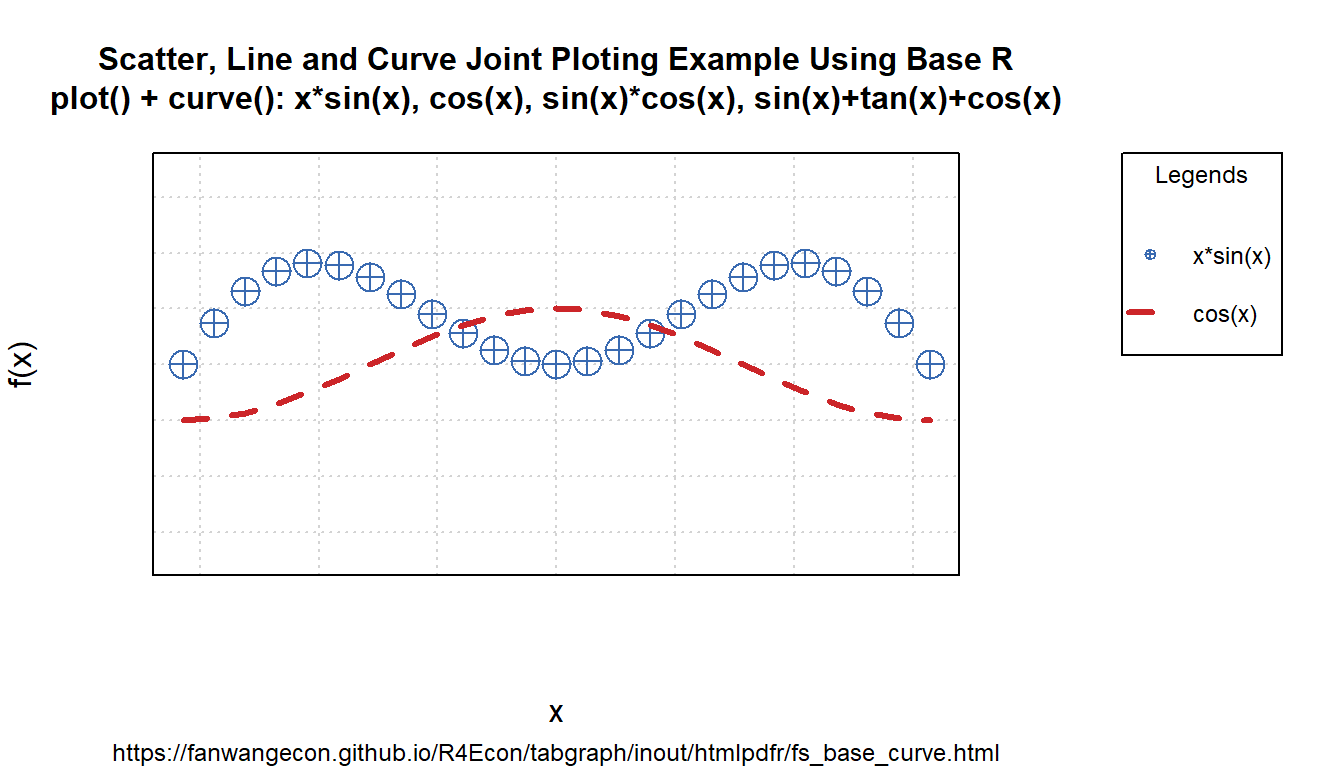
\includegraphics{Panel-Data-and-Optimization-with-R_files/figure-latex/unnamed-chunk-247-1} \end{center}

\begin{Shaded}
\begin{Highlighting}[]
\ControlFlowTok{if}\NormalTok{ (bl\_save\_img) \{}
  \FunctionTok{dev.off}\NormalTok{()}
\NormalTok{\}}
\end{Highlighting}
\end{Shaded}

\hypertarget{write-and-read-plots}{%
\section{Write and Read Plots}\label{write-and-read-plots}}

\hypertarget{import-and-export-images}{%
\subsection{Import and Export Images}\label{import-and-export-images}}

\begin{quote}
Go back to \href{http://fanwangecon.github.io/}{fan}'s \href{https://fanwangecon.github.io/REconTools/}{REconTools} Package, \href{https://fanwangecon.github.io/R4Econ/}{R Code Examples} Repository (\href{https://fanwangecon.github.io/R4Econ/bookdown}{bookdown site}), or \href{https://fanwangecon.github.io/Stat4Econ/}{Intro Stats with R} Repository (\href{https://fanwangecon.github.io/Stat4Econ/bookdown}{bookdown site}).
\end{quote}

Work with the R plot function.

\hypertarget{export-images-different-formats-with-plot}{%
\subsubsection{Export Images Different Formats with Plot()}\label{export-images-different-formats-with-plot}}

\hypertarget{generate-and-record-a-plot}{%
\paragraph{Generate and Record A Plot}\label{generate-and-record-a-plot}}

Generate a graph and recordPlot() it. The generated graph does not have legends Yet. Crucially, there are no titles, legends, axis, labels in the figures. As we stack the figures together, do not add those. Only add at the end jointly for all figure elements together to control at one spot things.

\begin{Shaded}
\begin{Highlighting}[]
\DocumentationTok{\#\#\#\#\#\#\#\#\#\#\#\#\#\#\#\#\#\#\#\#\#\#\#\#\#\#\#\#\#\#\#\#\#\#\#\#\#\#\#\#\#\#\#\#\#\#\#\#\#\#\#\#\#\#\#}
\CommentTok{\# First, Strings}
\DocumentationTok{\#\#\#\#\#\#\#\#\#\#\#\#\#\#\#\#\#\#\#\#\#\#\#\#\#\#\#\#\#\#\#\#\#\#\#\#\#\#\#\#\#\#\#\#\#\#\#\#\#\#\#\#\#\#\#}
\CommentTok{\# Labeling}
\NormalTok{st\_title }\OtherTok{\textless{}{-}} \FunctionTok{paste0}\NormalTok{(}\StringTok{\textquotesingle{}Scatter, Line and Curve Joint Ploting Example Using Base R}\SpecialCharTok{\textbackslash{}n}\StringTok{\textquotesingle{}}\NormalTok{,}
                   \StringTok{\textquotesingle{}plot() + curve():sin(x)*cos(x), sin(x)+tan(x)+cos(x)\textquotesingle{}}\NormalTok{)}
\NormalTok{st\_subtitle }\OtherTok{\textless{}{-}} \FunctionTok{paste0}\NormalTok{(}\StringTok{\textquotesingle{}https://fanwangecon.github.io/\textquotesingle{}}\NormalTok{,}
                      \StringTok{\textquotesingle{}R4Econ/tabgraph/inout/htmlpdfr/fs\_base\_curve.html\textquotesingle{}}\NormalTok{)}
\NormalTok{st\_x\_label }\OtherTok{\textless{}{-}} \StringTok{\textquotesingle{}x\textquotesingle{}}
\NormalTok{st\_y\_label }\OtherTok{\textless{}{-}} \StringTok{\textquotesingle{}f(x)\textquotesingle{}}

\DocumentationTok{\#\#\#\#\#\#\#\#\#\#\#\#\#\#\#\#\#\#\#\#\#\#\#\#\#\#\#\#\#\#\#\#\#\#\#\#\#\#\#\#\#\#\#\#\#\#\#\#\#\#\#\#\#\#\#}
\CommentTok{\# Second, functions}
\DocumentationTok{\#\#\#\#\#\#\#\#\#\#\#\#\#\#\#\#\#\#\#\#\#\#\#\#\#\#\#\#\#\#\#\#\#\#\#\#\#\#\#\#\#\#\#\#\#\#\#\#\#\#\#\#\#\#\#}
\NormalTok{fc\_sin\_cos\_diff }\OtherTok{\textless{}{-}} \ControlFlowTok{function}\NormalTok{(x) }\FunctionTok{sin}\NormalTok{(x)}\SpecialCharTok{*}\FunctionTok{cos}\NormalTok{(x)}
\NormalTok{st\_line\_3\_y\_legend }\OtherTok{\textless{}{-}} \StringTok{\textquotesingle{}sin(x)*cos(x)\textquotesingle{}}
\NormalTok{fc\_sin\_cos\_tan }\OtherTok{\textless{}{-}} \ControlFlowTok{function}\NormalTok{(x) }\FunctionTok{sin}\NormalTok{(x) }\SpecialCharTok{+} \FunctionTok{cos}\NormalTok{(x) }\SpecialCharTok{+} \FunctionTok{tan}\NormalTok{(x)}
\NormalTok{st\_line\_4\_y\_legend }\OtherTok{\textless{}{-}} \StringTok{\textquotesingle{}sin(x) + tan(x) + cos(x)\textquotesingle{}}

\DocumentationTok{\#\#\#\#\#\#\#\#\#\#\#\#\#\#\#\#\#\#\#\#\#\#\#\#\#\#\#\#\#\#\#\#\#\#\#\#\#\#\#\#\#\#\#\#\#\#\#\#\#\#\#\#\#\#\#}
\CommentTok{\# Third, patterns}
\DocumentationTok{\#\#\#\#\#\#\#\#\#\#\#\#\#\#\#\#\#\#\#\#\#\#\#\#\#\#\#\#\#\#\#\#\#\#\#\#\#\#\#\#\#\#\#\#\#\#\#\#\#\#\#\#\#\#\#}
\NormalTok{st\_line\_3\_black }\OtherTok{\textless{}{-}} \StringTok{\textquotesingle{}black\textquotesingle{}}
\NormalTok{st\_line\_4\_purple }\OtherTok{\textless{}{-}} \StringTok{\textquotesingle{}orange\textquotesingle{}}
\CommentTok{\# line type}
\NormalTok{st\_line\_3\_lty }\OtherTok{\textless{}{-}} \StringTok{\textquotesingle{}dotted\textquotesingle{}}
\NormalTok{st\_line\_4\_lty }\OtherTok{\textless{}{-}} \StringTok{\textquotesingle{}dotdash\textquotesingle{}}
\CommentTok{\# line width}
\NormalTok{st\_line\_3\_lwd }\OtherTok{\textless{}{-}} \FloatTok{2.5}
\NormalTok{st\_line\_4\_lwd }\OtherTok{\textless{}{-}} \FloatTok{3.5}

\DocumentationTok{\#\#\#\#\#\#\#\#\#\#\#\#\#\#\#\#\#\#\#\#\#\#\#\#\#\#\#\#\#\#\#\#\#\#\#\#\#\#\#\#\#\#\#\#\#\#\#\#\#\#\#\#\#\#\#}
\CommentTok{\# Fourth: Share xlim and ylim}
\DocumentationTok{\#\#\#\#\#\#\#\#\#\#\#\#\#\#\#\#\#\#\#\#\#\#\#\#\#\#\#\#\#\#\#\#\#\#\#\#\#\#\#\#\#\#\#\#\#\#\#\#\#\#\#\#\#\#\#}
\NormalTok{ar\_xlim }\OtherTok{=} \FunctionTok{c}\NormalTok{(}\SpecialCharTok{{-}}\DecValTok{3}\NormalTok{, }\DecValTok{3}\NormalTok{)}
\NormalTok{ar\_ylim }\OtherTok{=} \FunctionTok{c}\NormalTok{(}\SpecialCharTok{{-}}\FloatTok{3.5}\NormalTok{, }\FloatTok{3.5}\NormalTok{)}

\DocumentationTok{\#\#\#\#\#\#\#\#\#\#\#\#\#\#\#\#\#\#\#\#\#\#\#\#\#\#\#\#\#\#\#\#\#\#\#\#\#\#\#\#\#\#\#\#\#\#\#\#\#\#\#\#\#\#\#}
\CommentTok{\# Fifth: Even margins}
\DocumentationTok{\#\#\#\#\#\#\#\#\#\#\#\#\#\#\#\#\#\#\#\#\#\#\#\#\#\#\#\#\#\#\#\#\#\#\#\#\#\#\#\#\#\#\#\#\#\#\#\#\#\#\#\#\#\#\#}
\FunctionTok{par}\NormalTok{(}\AttributeTok{new=}\ConstantTok{FALSE}\NormalTok{)}

\DocumentationTok{\#\#\#\#\#\#\#\#\#\#\#\#\#\#\#\#\#\#\#\#\#\#\#\#\#\#\#\#\#\#\#\#\#\#\#\#\#\#\#\#\#\#\#\#\#\#\#\#\#\#\#\#\#\#\#}
\CommentTok{\# Sixth, the four objects and do not print yet:}
\DocumentationTok{\#\#\#\#\#\#\#\#\#\#\#\#\#\#\#\#\#\#\#\#\#\#\#\#\#\#\#\#\#\#\#\#\#\#\#\#\#\#\#\#\#\#\#\#\#\#\#\#\#\#\#\#\#\#\#}
\CommentTok{\# Graph Curve 3}
\FunctionTok{par}\NormalTok{(}\AttributeTok{new=}\NormalTok{T)}
\FunctionTok{curve}\NormalTok{(fc\_sin\_cos\_diff,}
      \AttributeTok{col =}\NormalTok{ st\_line\_3\_black,}
      \AttributeTok{lwd =}\NormalTok{ st\_line\_3\_lwd, }\AttributeTok{lty =}\NormalTok{ st\_line\_3\_lty,}
      \AttributeTok{from =}\NormalTok{ ar\_xlim[}\DecValTok{1}\NormalTok{], }\AttributeTok{to =}\NormalTok{ ar\_xlim[}\DecValTok{2}\NormalTok{], }\AttributeTok{ylim =}\NormalTok{ ar\_ylim,}
      \AttributeTok{ylab =} \StringTok{\textquotesingle{}\textquotesingle{}}\NormalTok{, }\AttributeTok{xlab =} \StringTok{\textquotesingle{}\textquotesingle{}}\NormalTok{, }\AttributeTok{yaxt=}\StringTok{\textquotesingle{}n\textquotesingle{}}\NormalTok{, }\AttributeTok{xaxt=}\StringTok{\textquotesingle{}n\textquotesingle{}}\NormalTok{, }\AttributeTok{ann=}\ConstantTok{FALSE}\NormalTok{)}
\CommentTok{\# Graph Curve 4}
\FunctionTok{par}\NormalTok{(}\AttributeTok{new=}\NormalTok{T)}
\FunctionTok{curve}\NormalTok{(fc\_sin\_cos\_tan,}
      \AttributeTok{col =}\NormalTok{ st\_line\_4\_purple,}
      \AttributeTok{lwd =}\NormalTok{ st\_line\_4\_lwd, }\AttributeTok{lty =}\NormalTok{ st\_line\_4\_lty,}
      \AttributeTok{from =}\NormalTok{ ar\_xlim[}\DecValTok{1}\NormalTok{], }\AttributeTok{to =}\NormalTok{ ar\_xlim[}\DecValTok{2}\NormalTok{], }\AttributeTok{ylim =}\NormalTok{ ar\_ylim,}
      \AttributeTok{ylab =} \StringTok{\textquotesingle{}\textquotesingle{}}\NormalTok{, }\AttributeTok{xlab =} \StringTok{\textquotesingle{}\textquotesingle{}}\NormalTok{, }\AttributeTok{yaxt=}\StringTok{\textquotesingle{}n\textquotesingle{}}\NormalTok{, }\AttributeTok{xaxt=}\StringTok{\textquotesingle{}n\textquotesingle{}}\NormalTok{, }\AttributeTok{ann=}\ConstantTok{FALSE}\NormalTok{)}
\end{Highlighting}
\end{Shaded}

\begin{Shaded}
\begin{Highlighting}[]
\NormalTok{pl\_curves\_save }\OtherTok{\textless{}{-}} \FunctionTok{recordPlot}\NormalTok{()}
\end{Highlighting}
\end{Shaded}

\hypertarget{generate-large-font-and-small-font-versions-of-plot}{%
\paragraph{Generate Large Font and Small Font Versions of PLot}\label{generate-large-font-and-small-font-versions-of-plot}}

Generate larger font version:

\begin{Shaded}
\begin{Highlighting}[]
\CommentTok{\# Replay}
\NormalTok{pl\_curves\_save}

\DocumentationTok{\#\#\#\#\#\#\#\#\#\#\#\#\#\#\#\#\#\#\#\#\#\#\#\#\#\#\#\#\#\#\#\#\#\#\#\#\#\#\#\#\#\#\#\#\#\#\#\#\#\#\#\#\#\#\#}
\CommentTok{\# Seventh, Set Title and Legend and Plot Jointly}
\DocumentationTok{\#\#\#\#\#\#\#\#\#\#\#\#\#\#\#\#\#\#\#\#\#\#\#\#\#\#\#\#\#\#\#\#\#\#\#\#\#\#\#\#\#\#\#\#\#\#\#\#\#\#\#\#\#\#\#}
\CommentTok{\# CEX sizing Contorl Titling and Legend Sizes}
\NormalTok{fl\_ces\_fig\_reg }\OtherTok{=} \FloatTok{0.75}
\NormalTok{fl\_ces\_fig\_leg }\OtherTok{=} \FloatTok{0.75}
\NormalTok{fl\_ces\_fig\_small }\OtherTok{=} \FloatTok{0.65}

\CommentTok{\# R Legend}
\FunctionTok{title}\NormalTok{(}\AttributeTok{main =}\NormalTok{ st\_title, }\AttributeTok{sub =}\NormalTok{ st\_subtitle, }\AttributeTok{xlab =}\NormalTok{ st\_x\_label, }\AttributeTok{ylab =}\NormalTok{ st\_y\_label,}
      \AttributeTok{cex.lab=}\NormalTok{fl\_ces\_fig\_reg,}
      \AttributeTok{cex.main=}\NormalTok{fl\_ces\_fig\_reg,}
      \AttributeTok{cex.sub=}\NormalTok{fl\_ces\_fig\_small)}
\FunctionTok{axis}\NormalTok{(}\DecValTok{1}\NormalTok{, }\AttributeTok{cex.axis=}\NormalTok{fl\_ces\_fig\_reg)}
\FunctionTok{axis}\NormalTok{(}\DecValTok{2}\NormalTok{, }\AttributeTok{cex.axis=}\NormalTok{fl\_ces\_fig\_reg)}
\FunctionTok{grid}\NormalTok{()}

\CommentTok{\# Legend sizing CEX}
\FunctionTok{legend}\NormalTok{(}\StringTok{"topleft"}\NormalTok{,}
       \AttributeTok{bg=}\StringTok{"transparent"}\NormalTok{,}
       \AttributeTok{bty =} \StringTok{"n"}\NormalTok{,}
       \FunctionTok{c}\NormalTok{(st\_line\_3\_y\_legend, st\_line\_4\_y\_legend),}
       \AttributeTok{col =} \FunctionTok{c}\NormalTok{(st\_line\_3\_black, st\_line\_4\_purple),}
       \AttributeTok{pch =} \FunctionTok{c}\NormalTok{(}\ConstantTok{NA}\NormalTok{, }\ConstantTok{NA}\NormalTok{),}
       \AttributeTok{cex =}\NormalTok{ fl\_ces\_fig\_leg,}
       \AttributeTok{lty =} \FunctionTok{c}\NormalTok{(st\_line\_3\_lty, st\_line\_4\_lty),}
       \AttributeTok{lwd =} \FunctionTok{c}\NormalTok{(st\_line\_3\_lwd,st\_line\_4\_lwd),}
       \AttributeTok{y.intersp=}\DecValTok{2}\NormalTok{)}
\end{Highlighting}
\end{Shaded}

\begin{Shaded}
\begin{Highlighting}[]
\CommentTok{\# record final plot}
\NormalTok{pl\_curves\_large }\OtherTok{\textless{}{-}} \FunctionTok{recordPlot}\NormalTok{()}
\FunctionTok{dev.off}\NormalTok{()}
\end{Highlighting}
\end{Shaded}

Generate smaller font version:

\begin{Shaded}
\begin{Highlighting}[]
\CommentTok{\# Replay}
\NormalTok{pl\_curves\_save}

\DocumentationTok{\#\#\#\#\#\#\#\#\#\#\#\#\#\#\#\#\#\#\#\#\#\#\#\#\#\#\#\#\#\#\#\#\#\#\#\#\#\#\#\#\#\#\#\#\#\#\#\#\#\#\#\#\#\#\#}
\CommentTok{\# Seventh, Set Title and Legend and Plot Jointly}
\DocumentationTok{\#\#\#\#\#\#\#\#\#\#\#\#\#\#\#\#\#\#\#\#\#\#\#\#\#\#\#\#\#\#\#\#\#\#\#\#\#\#\#\#\#\#\#\#\#\#\#\#\#\#\#\#\#\#\#}
\CommentTok{\# CEX sizing Contorl Titling and Legend Sizes}
\NormalTok{fl\_ces\_fig\_reg }\OtherTok{=} \FloatTok{0.45}
\NormalTok{fl\_ces\_fig\_leg }\OtherTok{=} \FloatTok{0.45}
\NormalTok{fl\_ces\_fig\_small }\OtherTok{=} \FloatTok{0.25}

\CommentTok{\# R Legend}
\FunctionTok{title}\NormalTok{(}\AttributeTok{main =}\NormalTok{ st\_title, }\AttributeTok{sub =}\NormalTok{ st\_subtitle, }\AttributeTok{xlab =}\NormalTok{ st\_x\_label, }\AttributeTok{ylab =}\NormalTok{ st\_y\_label,}
      \AttributeTok{cex.lab=}\NormalTok{fl\_ces\_fig\_reg,}
      \AttributeTok{cex.main=}\NormalTok{fl\_ces\_fig\_reg,}
      \AttributeTok{cex.sub=}\NormalTok{fl\_ces\_fig\_small)}
\FunctionTok{axis}\NormalTok{(}\DecValTok{1}\NormalTok{, }\AttributeTok{cex.axis=}\NormalTok{fl\_ces\_fig\_reg)}
\FunctionTok{axis}\NormalTok{(}\DecValTok{2}\NormalTok{, }\AttributeTok{cex.axis=}\NormalTok{fl\_ces\_fig\_reg)}
\FunctionTok{grid}\NormalTok{()}

\CommentTok{\# Legend sizing CEX}
\FunctionTok{legend}\NormalTok{(}\StringTok{"topleft"}\NormalTok{,}
       \AttributeTok{bg=}\StringTok{"transparent"}\NormalTok{,}
       \AttributeTok{bty =} \StringTok{"n"}\NormalTok{,}
       \FunctionTok{c}\NormalTok{(st\_line\_3\_y\_legend, st\_line\_4\_y\_legend),}
       \AttributeTok{col =} \FunctionTok{c}\NormalTok{(st\_line\_3\_black, st\_line\_4\_purple),}
       \AttributeTok{pch =} \FunctionTok{c}\NormalTok{(}\ConstantTok{NA}\NormalTok{, }\ConstantTok{NA}\NormalTok{),}
       \AttributeTok{cex =}\NormalTok{ fl\_ces\_fig\_leg,}
       \AttributeTok{lty =} \FunctionTok{c}\NormalTok{(st\_line\_3\_lty, st\_line\_4\_lty),}
       \AttributeTok{lwd =} \FunctionTok{c}\NormalTok{(st\_line\_3\_lwd,st\_line\_4\_lwd),}
       \AttributeTok{y.intersp=}\DecValTok{2}\NormalTok{)}
\end{Highlighting}
\end{Shaded}

\begin{Shaded}
\begin{Highlighting}[]
\CommentTok{\# record final plot}
\NormalTok{pl\_curves\_small }\OtherTok{\textless{}{-}} \FunctionTok{recordPlot}\NormalTok{()}
\FunctionTok{dev.off}\NormalTok{()}
\end{Highlighting}
\end{Shaded}

\hypertarget{save-plot-with-varying-resolutions-and-heights}{%
\paragraph{Save Plot with Varying Resolutions and Heights}\label{save-plot-with-varying-resolutions-and-heights}}

Export recorded plot.

A4 paper is 8.3 x 11.7, with 1 inch margins, the remaining area is 6.3 x 9.7. For figures that should take half of the page, the height should be 4.8 inch. One third of a page should be 3.2 inch. 6.3 inch is 160mm and 3 inch is 76 mm. In the example below, use

\begin{Shaded}
\begin{Highlighting}[]
\CommentTok{\# Store both in within folder directory and root image directory:}
\CommentTok{\# C:\textbackslash{}Users\textbackslash{}fan\textbackslash{}R4Econ\textbackslash{}tabgraph\textbackslash{}inout\textbackslash{}\_img}
\CommentTok{\# C:\textbackslash{}Users\textbackslash{}fan\textbackslash{}R4Econ\textbackslash{}\_img}
\CommentTok{\# need to store in both because bookdown and indi pdf path differ.}
\CommentTok{\# Wrap in try because will not work underbookdown, but images already created}

\NormalTok{ls\_spt\_root }\OtherTok{\textless{}{-}} \FunctionTok{c}\NormalTok{(}\StringTok{\textquotesingle{}..//..//\textquotesingle{}}\NormalTok{, }\StringTok{\textquotesingle{}\textquotesingle{}}\NormalTok{)}
\NormalTok{spt\_prefix }\OtherTok{\textless{}{-}} \StringTok{\textquotesingle{}\_img/fs\_img\_io\_2curve\textquotesingle{}}

\ControlFlowTok{for}\NormalTok{ (spt\_root }\ControlFlowTok{in}\NormalTok{ ls\_spt\_root) \{}
  \CommentTok{\# Changing pointsize will not change font sizes inside, just rescale}
  \CommentTok{\# PNG 72}
  \FunctionTok{try}\NormalTok{(}\FunctionTok{png}\NormalTok{(}\FunctionTok{paste0}\NormalTok{(spt\_root, spt\_prefix, }\StringTok{"\_w135h76\_res72.png"}\NormalTok{),}
      \AttributeTok{width =} \DecValTok{135}\NormalTok{ , }\AttributeTok{height =} \DecValTok{76}\NormalTok{, }\AttributeTok{units=}\StringTok{\textquotesingle{}mm\textquotesingle{}}\NormalTok{, }\AttributeTok{res =} \DecValTok{72}\NormalTok{, }\AttributeTok{pointsize=}\DecValTok{7}\NormalTok{))}
  \FunctionTok{print}\NormalTok{(pl\_curves\_large)}
  \FunctionTok{dev.off}\NormalTok{()}
  \CommentTok{\# PNG 300}
  \FunctionTok{try}\NormalTok{(}\FunctionTok{png}\NormalTok{(}\FunctionTok{paste0}\NormalTok{(spt\_root, spt\_prefix, }\StringTok{"\_w135h76\_res300.png"}\NormalTok{),}
      \AttributeTok{width =} \DecValTok{135}\NormalTok{, }\AttributeTok{height =} \DecValTok{76}\NormalTok{, }\AttributeTok{units=}\StringTok{\textquotesingle{}mm\textquotesingle{}}\NormalTok{, }\AttributeTok{res =} \DecValTok{300}\NormalTok{, }\AttributeTok{pointsize=}\DecValTok{7}\NormalTok{))}
  \FunctionTok{print}\NormalTok{(pl\_curves\_large)}
  \FunctionTok{dev.off}\NormalTok{()}
  \CommentTok{\# PNG 300, SMALL, POINT SIZE LOWER}
  \FunctionTok{try}\NormalTok{(}\FunctionTok{png}\NormalTok{(}\FunctionTok{paste0}\NormalTok{(spt\_root, spt\_prefix, }\StringTok{"\_w80h48\_res300.png"}\NormalTok{),}
      \AttributeTok{width =} \DecValTok{80}\NormalTok{, }\AttributeTok{height =} \DecValTok{48}\NormalTok{, }\AttributeTok{units=}\StringTok{\textquotesingle{}mm\textquotesingle{}}\NormalTok{, }\AttributeTok{res =} \DecValTok{300}\NormalTok{, }\AttributeTok{pointsize=}\DecValTok{7}\NormalTok{))}
  \FunctionTok{print}\NormalTok{(pl\_curves\_small)}
  \FunctionTok{dev.off}\NormalTok{()}
  \CommentTok{\# PNG 300}
  \FunctionTok{try}\NormalTok{(}\FunctionTok{png}\NormalTok{(}\FunctionTok{paste0}\NormalTok{(spt\_root, spt\_prefix, }\StringTok{"\_w160h100\_res300.png"}\NormalTok{),}
      \AttributeTok{width =} \DecValTok{160}\NormalTok{, }\AttributeTok{height =} \DecValTok{100}\NormalTok{, }\AttributeTok{units=}\StringTok{\textquotesingle{}mm\textquotesingle{}}\NormalTok{, }\AttributeTok{res =} \DecValTok{300}\NormalTok{))}
  \FunctionTok{print}\NormalTok{(pl\_curves\_large)}
  \FunctionTok{dev.off}\NormalTok{()}

  \CommentTok{\# EPS}
  \FunctionTok{setEPS}\NormalTok{()}
  \FunctionTok{try}\NormalTok{(}\FunctionTok{postscript}\NormalTok{(}\FunctionTok{paste0}\NormalTok{(spt\_root, spt\_prefix, }\StringTok{"\_fs\_2curve.eps"}\NormalTok{)))}
  \FunctionTok{print}\NormalTok{(pl\_curves\_large)}
  \FunctionTok{dev.off}\NormalTok{()}
\NormalTok{\}}
\end{Highlighting}
\end{Shaded}

\begin{verbatim}
## Error in png(paste0(spt_root, spt_prefix, "_w135h76_res72.png"), width = 135,  : 
##   unable to start png() device
## Error in png(paste0(spt_root, spt_prefix, "_w135h76_res300.png"), width = 135,  : 
##   unable to start png() device
## Error in png(paste0(spt_root, spt_prefix, "_w80h48_res300.png"), width = 80,  : 
##   unable to start png() device
## Error in png(paste0(spt_root, spt_prefix, "_w160h100_res300.png"), width = 160,  : 
##   unable to start png() device
## Error in postscript(paste0(spt_root, spt_prefix, "_fs_2curve.eps")) : 
##   cannot open file '..//..//_img/fs_img_io_2curve_fs_2curve.eps'
\end{verbatim}

\hypertarget{low-and-high-resolution-figure}{%
\paragraph{Low and High Resolution Figure}\label{low-and-high-resolution-figure}}

The standard resolution often produces very low quality images. Resolution should be increased. See figure comparison.

\begin{figure}
\centering
\caption{RES=72 (DEFAULT R) TOP, RES=300 Bottom, (Width=160, Height=81, PNG)}
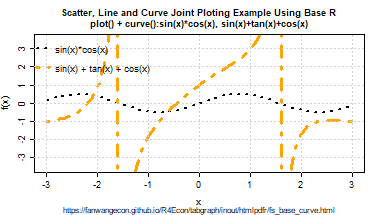
\includegraphics[width=\linewidth]{_img/fs_img_io_2curve_w135h76_res72.png}
\hfill
\centering
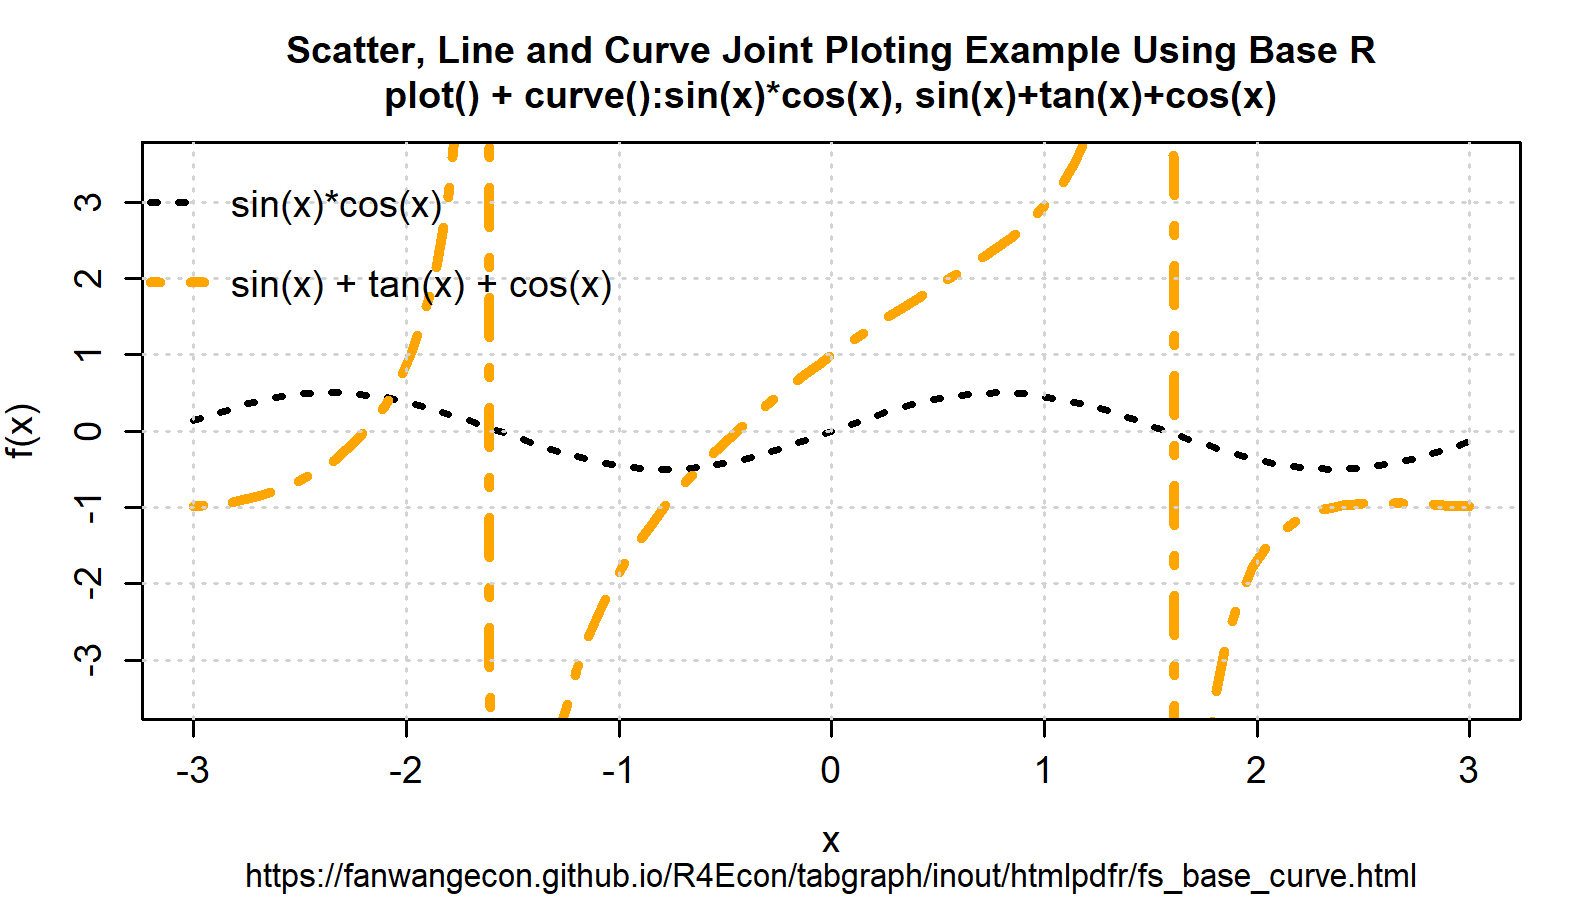
\includegraphics[width=\linewidth]{_img/fs_img_io_2curve_w135h76_res300.png}
\end{figure}

\hypertarget{smaller-and-larger-figures}{%
\paragraph{Smaller and Larger Figures}\label{smaller-and-larger-figures}}

Smaller and larger figures with different font size comparison. Note that earlier, we generated the figure without legends, labels, etc first, recorded the figure. Then we associated the same underlying figure with differently sized titles, legends, axis, labels.

\begin{figure}
\centering
\caption{Top Small (small font saved), Bottom Large, PNG}
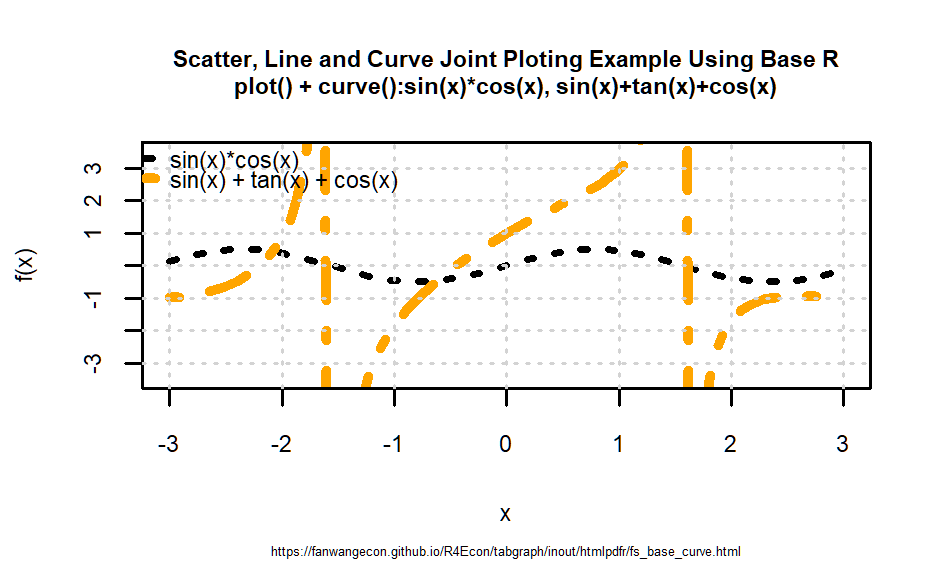
\includegraphics[width=\linewidth]{_img/fs_img_io_2curve_w80h48_res300.png}
\hfill
\centering
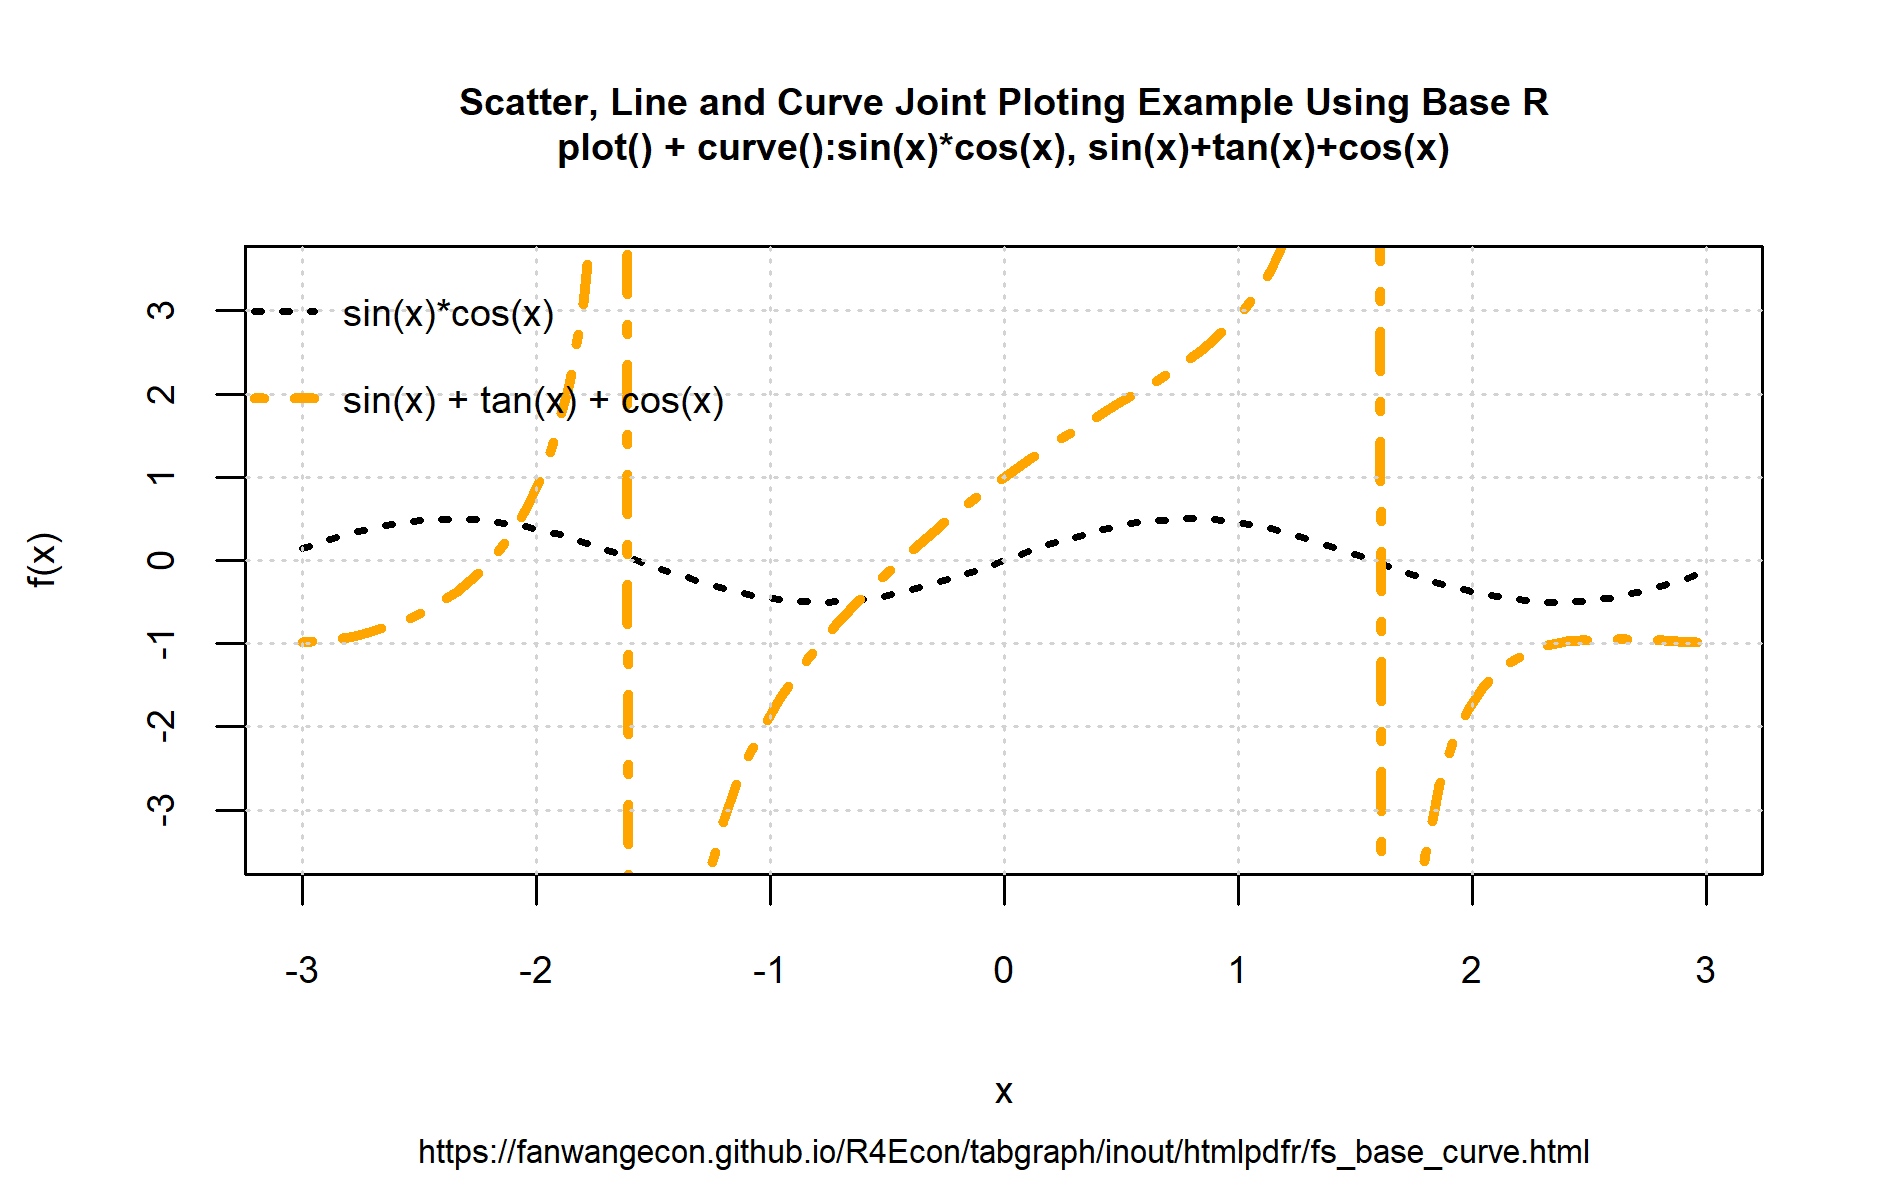
\includegraphics[width=\linewidth]{_img/fs_img_io_2curve_w160h100_res300.png}
\end{figure}

\hypertarget{get-data}{%
\chapter{Get Data}\label{get-data}}

\hypertarget{environmental-data}{%
\section{Environmental Data}\label{environmental-data}}

\hypertarget{ecmwf-era5-data}{%
\subsection{ECMWF ERA5 Data}\label{ecmwf-era5-data}}

\begin{quote}
Go back to \href{http://fanwangecon.github.io/}{fan}'s \href{https://fanwangecon.github.io/REconTools/}{REconTools} Package, \href{https://fanwangecon.github.io/R4Econ/}{R Code Examples} Repository (\href{https://fanwangecon.github.io/R4Econ/bookdown}{bookdown site}), or \href{https://fanwangecon.github.io/Stat4Econ/}{Intro Stats with R} Repository (\href{https://fanwangecon.github.io/Stat4Econ/bookdown}{bookdown site}).
\end{quote}

This files uses R with the reticulate package to download ECMWF ERA5 data. See \href{https://fanwangecon.github.io/pyfan/vig/getdata/envir/htmlpdfr/fs_ecmwf.html}{this file} for instructions and tutorials for downloading the data.

\hypertarget{program-to-download-unzip-convert-to-combined-csv-derived-utci-historical-data}{%
\subsubsection{Program to Download, Unzip, Convert to combined CSV, derived-utci-historical data}\label{program-to-download-unzip-convert-to-combined-csv-derived-utci-historical-data}}

The data downloaded from CDS climate could become very large in size. We want to process parts of the data one part at a time, summarize and aggregate over each part, and generate a file output file with aggregate statistics over the entire time period of interest.

This code below accompalishes the following tasks:

\begin{enumerate}
\def\labelenumi{\arabic{enumi}.}
\tightlist
\item
  download data from derived-utci-historical as ZIP
\item
  unzip
\item
  convert \emph{nc} files to \emph{csv} files
\item
  individual csv files are half year groups
\end{enumerate}

Parameter Control for the code below:

\begin{enumerate}
\def\labelenumi{\arabic{enumi}.}
\tightlist
\item
  \emph{spt\_root}: root folder where everything will be at
\item
  \emph{spth\_conda\_env}: the conda virtual environment python path, eccodes and cdsapi packages are installed in the conda virtual environment. In the example below, the first env is: wk\_ecmwf
\item
  \emph{st\_nc\_prefix}: the downloaded individual nc files have dates and prefix before and after the date string in the nc file names. This is the string before that.
\item
  \emph{st\_nc\_suffix}: see (3), this is the suffix
\item
  \emph{ar\_years}: array of years to download and aggregate over
\item
  \emph{ar\_months\_g1}: months to download in first half year
\item
  \emph{ar\_months\_g2}: months to download in second half year
\end{enumerate}

Note: \emph{area} below corresponds to \emph{North, West, South, East}.

\begin{Shaded}
\begin{Highlighting}[]
\DocumentationTok{\#\#\#\#\#\#\#\#\#\#\#\#\#\#\#\#\#\#\#\#\#\#\#\#\#\#\#\#\#\#\#\#\#\#\#\#\#\#\#\#\#\#\#\#\#\#\#\#\#}
\CommentTok{\# {-}{-}{-}{-}{-}{-}{-}{-}{-}{-}{-}{-} Parameters}
\DocumentationTok{\#\#\#\#\#\#\#\#\#\#\#\#\#\#\#\#\#\#\#\#\#\#\#\#\#\#\#\#\#\#\#\#\#\#\#\#\#\#\#\#\#\#\#\#\#\#\#\#\#}

\CommentTok{\# Where to store everything}
\NormalTok{spt\_root }\OtherTok{\textless{}{-}} \StringTok{"C:/Users/fan/Downloads/\_data/"}
\NormalTok{spth\_conda\_env }\OtherTok{\textless{}{-}} \StringTok{"C:/ProgramData/Anaconda3/envs/wk\_ecmwf/python.exe"}

\CommentTok{\# nc name prefix}
\NormalTok{st\_nc\_prefix }\OtherTok{\textless{}{-}} \StringTok{"ECMWF\_utci\_"}
\NormalTok{st\_nc\_suffix }\OtherTok{\textless{}{-}} \StringTok{"\_v1.0\_con.nc"}

\CommentTok{\# Years list}
\CommentTok{\# ar\_years \textless{}{-} 2001:2019}
\NormalTok{ar\_years }\OtherTok{\textless{}{-}} \FunctionTok{c}\NormalTok{(}\DecValTok{2005}\NormalTok{, }\DecValTok{2015}\NormalTok{)}
\CommentTok{\# ar\_months\_g1 \textless{}{-} c(\textquotesingle{}01\textquotesingle{},\textquotesingle{}02\textquotesingle{},\textquotesingle{}03\textquotesingle{},\textquotesingle{}04\textquotesingle{},\textquotesingle{}05\textquotesingle{},\textquotesingle{}06\textquotesingle{})}
\NormalTok{ar\_months\_g1 }\OtherTok{\textless{}{-}} \FunctionTok{c}\NormalTok{(}\StringTok{\textquotesingle{}01\textquotesingle{}}\NormalTok{, }\StringTok{\textquotesingle{}03\textquotesingle{}}\NormalTok{)}
\CommentTok{\# ar\_months\_g2 \textless{}{-} c(\textquotesingle{}07\textquotesingle{},\textquotesingle{}08\textquotesingle{},\textquotesingle{}09\textquotesingle{},\textquotesingle{}10\textquotesingle{},\textquotesingle{}11\textquotesingle{},\textquotesingle{}12\textquotesingle{})}
\NormalTok{ar\_months\_g2 }\OtherTok{\textless{}{-}} \FunctionTok{c}\NormalTok{(}\StringTok{\textquotesingle{}07\textquotesingle{}}\NormalTok{, }\StringTok{\textquotesingle{}09\textquotesingle{}}\NormalTok{)}

\CommentTok{\# Area}
\CommentTok{\# \# China}
\CommentTok{\# fl\_area\_north \textless{}{-} 53.31}
\CommentTok{\# fl\_area\_west \textless{}{-} 73}
\CommentTok{\# fl\_area\_south \textless{}{-} 4.15}
\CommentTok{\# fl\_area\_east \textless{}{-} 135}
\NormalTok{fl\_area\_north }\OtherTok{\textless{}{-}} \DecValTok{53}
\NormalTok{fl\_area\_west }\OtherTok{\textless{}{-}} \DecValTok{73}
\NormalTok{fl\_area\_south }\OtherTok{\textless{}{-}} \DecValTok{52}
\NormalTok{fl\_area\_east }\OtherTok{\textless{}{-}} \DecValTok{74}

\CommentTok{\# folder to download any nc zips to}
\NormalTok{nczippath }\OtherTok{\textless{}{-}}\NormalTok{ spt\_root}
\CommentTok{\# we are changing the python api file with different requests stirngs and storing it here}
\NormalTok{pyapipath }\OtherTok{\textless{}{-}}\NormalTok{ spt\_root}
\CommentTok{\# output directory for AGGREGATE CSV with all DATES from this search}
\NormalTok{csvpath }\OtherTok{\textless{}{-}}\NormalTok{ spt\_root}

\DocumentationTok{\#\#\#\#\#\#\#\#\#\#\#\#\#\#\#\#\#\#\#\#\#\#\#\#\#\#\#\#\#\#\#\#\#\#\#\#\#\#\#\#\#\#\#\#\#\#\#\#\#}
\CommentTok{\# {-}{-}{-}{-}{-}{-}{-}{-}{-}{-}{-}{-} Packages}
\DocumentationTok{\#\#\#\#\#\#\#\#\#\#\#\#\#\#\#\#\#\#\#\#\#\#\#\#\#\#\#\#\#\#\#\#\#\#\#\#\#\#\#\#\#\#\#\#\#\#\#\#\#}

\FunctionTok{library}\NormalTok{(}\StringTok{"ncdf4"}\NormalTok{)}
\FunctionTok{library}\NormalTok{(}\StringTok{"chron"}\NormalTok{)}
\FunctionTok{library}\NormalTok{(}\StringTok{"lattice"}\NormalTok{)}
\FunctionTok{library}\NormalTok{(}\StringTok{"RColorBrewer"}\NormalTok{)}
\FunctionTok{library}\NormalTok{(}\StringTok{"stringr"}\NormalTok{)}
\FunctionTok{library}\NormalTok{(}\StringTok{"tibble"}\NormalTok{)}
\FunctionTok{library}\NormalTok{(}\StringTok{"dplyr"}\NormalTok{)}
\FunctionTok{Sys.setenv}\NormalTok{(}\AttributeTok{RETICULATE\_PYTHON =}\NormalTok{ spth\_conda\_env)}
\FunctionTok{library}\NormalTok{(}\StringTok{"reticulate"}\NormalTok{)}

\DocumentationTok{\#\#\#\#\#\#\#\#\#\#\#\#\#\#\#\#\#\#\#\#\#\#\#\#\#\#\#\#\#\#\#\#\#\#\#\#\#\#\#\#\#\#\#\#\#\#\#\#\#}
\CommentTok{\# {-}{-}{-}{-}{-}{-}{-}{-}{-}{-}{-}{-} Define Loops}
\DocumentationTok{\#\#\#\#\#\#\#\#\#\#\#\#\#\#\#\#\#\#\#\#\#\#\#\#\#\#\#\#\#\#\#\#\#\#\#\#\#\#\#\#\#\#\#\#\#\#\#\#\#}
\ControlFlowTok{for}\NormalTok{ (it\_yr }\ControlFlowTok{in}\NormalTok{ ar\_years) \{}
  \ControlFlowTok{for}\NormalTok{ (it\_mth\_group }\ControlFlowTok{in} \FunctionTok{c}\NormalTok{(}\DecValTok{1}\NormalTok{,}\DecValTok{2}\NormalTok{)) \{}
    \ControlFlowTok{if}\NormalTok{(it\_mth\_group }\SpecialCharTok{==} \DecValTok{1}\NormalTok{) \{}
\NormalTok{      ar\_months }\OtherTok{=}\NormalTok{ ar\_months\_g1}
\NormalTok{    \}}
    \ControlFlowTok{if}\NormalTok{(it\_mth\_group }\SpecialCharTok{==} \DecValTok{2}\NormalTok{) \{}
\NormalTok{      ar\_months }\OtherTok{=}\NormalTok{ ar\_months\_g2}
\NormalTok{    \}}

    \DocumentationTok{\#\#\#\#\#\#\#\#\#\#\#\#\#\#\#\#\#\#\#\#\#\#\#\#\#\#\#\#\#\#\#\#\#\#\#\#\#\#\#\#\#\#\#\#\#\#\#\#\#}
    \CommentTok{\# {-}{-}{-}{-}{-}{-}{-}{-}{-}{-}{-}{-} Define Python API Call}
    \DocumentationTok{\#\#\#\#\#\#\#\#\#\#\#\#\#\#\#\#\#\#\#\#\#\#\#\#\#\#\#\#\#\#\#\#\#\#\#\#\#\#\#\#\#\#\#\#\#\#\#\#\#}

    \CommentTok{\# name of zip file}
\NormalTok{    nczipname }\OtherTok{\textless{}{-}} \StringTok{"derived\_utci\_2010\_2.zip"}
\NormalTok{    unzipfolder }\OtherTok{\textless{}{-}} \StringTok{"derived\_utci\_2010\_2"}

\NormalTok{    st\_file }\OtherTok{\textless{}{-}} \FunctionTok{paste0}\NormalTok{(}\StringTok{"import cdsapi}
\StringTok{import urllib.request}
\StringTok{\# download folder}
\StringTok{spt\_root = \textquotesingle{}"}\NormalTok{, nczippath, }\StringTok{"\textquotesingle{}}
\StringTok{spn\_dl\_test\_grib = spt\_root + \textquotesingle{}"}\NormalTok{, nczipname, }\StringTok{"\textquotesingle{}}
\StringTok{\# request}
\StringTok{c = cdsapi.Client()}
\StringTok{res = c.retrieve(}
\StringTok{    \textquotesingle{}derived{-}utci{-}historical\textquotesingle{},}
\StringTok{    \{}
\StringTok{        \textquotesingle{}format\textquotesingle{}: \textquotesingle{}zip\textquotesingle{},}
\StringTok{        \textquotesingle{}variable\textquotesingle{}: \textquotesingle{}Universal thermal climate index\textquotesingle{},}
\StringTok{        \textquotesingle{}product\_type\textquotesingle{}: \textquotesingle{}Consolidated dataset\textquotesingle{},}
\StringTok{        \textquotesingle{}year\textquotesingle{}: \textquotesingle{}"}\NormalTok{,it\_yr, }\StringTok{"\textquotesingle{},}
\StringTok{        \textquotesingle{}month\textquotesingle{}: [}
\StringTok{            "}\NormalTok{, }\FunctionTok{paste}\NormalTok{(}\StringTok{"\textquotesingle{}"}\NormalTok{, ar\_months, }\StringTok{"\textquotesingle{}"}\NormalTok{, }\AttributeTok{sep =} \StringTok{""}\NormalTok{, }\AttributeTok{collapse =} \StringTok{", "}\NormalTok{), }\StringTok{"}
\StringTok{        ],}
\StringTok{        \textquotesingle{}day\textquotesingle{}: [}
\StringTok{            \textquotesingle{}01\textquotesingle{},\textquotesingle{}03\textquotesingle{}}
\StringTok{        ],}
\StringTok{        \textquotesingle{}area\textquotesingle{}  : ["}\NormalTok{, fl\_area\_north ,}\StringTok{", "}\NormalTok{, fl\_area\_west ,}\StringTok{", "}\NormalTok{, fl\_area\_south ,}\StringTok{", "}\NormalTok{, fl\_area\_east ,}\StringTok{"],}
\StringTok{        \textquotesingle{}grid\textquotesingle{}  : [0.25, 0.25],}
\StringTok{    \},}
\StringTok{    spn\_dl\_test\_grib)}
\StringTok{\# show results}
\StringTok{print(\textquotesingle{}print results\textquotesingle{})}
\StringTok{print(res)}
\StringTok{print(type(res))"}\NormalTok{)}

    \CommentTok{\# st\_file = "print(1+1)"}

    \CommentTok{\# Store Python Api File}
\NormalTok{    fl\_test\_tex }\OtherTok{\textless{}{-}} \FunctionTok{paste0}\NormalTok{(pyapipath, }\StringTok{"api.py"}\NormalTok{)}
\NormalTok{    fileConn }\OtherTok{\textless{}{-}} \FunctionTok{file}\NormalTok{(fl\_test\_tex)}
    \FunctionTok{writeLines}\NormalTok{(st\_file, fileConn)}
    \FunctionTok{close}\NormalTok{(fileConn)}

    \DocumentationTok{\#\#\#\#\#\#\#\#\#\#\#\#\#\#\#\#\#\#\#\#\#\#\#\#\#\#\#\#\#\#\#\#\#\#\#\#\#\#\#\#\#\#\#\#\#\#\#\#\#}
    \CommentTok{\# {-}{-}{-}{-}{-}{-}{-}{-}{-}{-}{-}{-} Run Python File}
    \DocumentationTok{\#\#\#\#\#\#\#\#\#\#\#\#\#\#\#\#\#\#\#\#\#\#\#\#\#\#\#\#\#\#\#\#\#\#\#\#\#\#\#\#\#\#\#\#\#\#\#\#\#}
    \CommentTok{\# Set Path}
    \FunctionTok{setwd}\NormalTok{(pyapipath)}
    \CommentTok{\# Run py file, api.py name just defined}
    \FunctionTok{use\_python}\NormalTok{(spth\_conda\_env)}
    \FunctionTok{source\_python}\NormalTok{(}\StringTok{\textquotesingle{}api.py\textquotesingle{}}\NormalTok{)}

    \DocumentationTok{\#\#\#\#\#\#\#\#\#\#\#\#\#\#\#\#\#\#\#\#\#\#\#\#\#\#\#\#\#\#\#\#\#\#\#\#\#\#\#\#\#\#\#\#\#\#\#\#\#}
    \CommentTok{\# {-}{-}{-}{-}{-}{-}{-}{-}{-}{-}{-}{-} uNZIP}
    \DocumentationTok{\#\#\#\#\#\#\#\#\#\#\#\#\#\#\#\#\#\#\#\#\#\#\#\#\#\#\#\#\#\#\#\#\#\#\#\#\#\#\#\#\#\#\#\#\#\#\#\#\#}
\NormalTok{    spn\_zip }\OtherTok{\textless{}{-}} \FunctionTok{paste0}\NormalTok{(nczippath, nczipname)}
\NormalTok{    spn\_unzip\_folder }\OtherTok{\textless{}{-}} \FunctionTok{paste0}\NormalTok{(nczippath, unzipfolder)}
    \FunctionTok{unzip}\NormalTok{(spn\_zip, }\AttributeTok{exdir=}\NormalTok{spn\_unzip\_folder)}

    \DocumentationTok{\#\#\#\#\#\#\#\#\#\#\#\#\#\#\#\#\#\#\#\#\#\#\#\#\#\#\#\#\#\#\#\#\#\#\#\#\#\#\#\#\#\#\#\#\#\#\#\#\#}
    \CommentTok{\# {-}{-}{-}{-}{-}{-}{-}{-}{-}{-}{-}{-} Find All files}
    \DocumentationTok{\#\#\#\#\#\#\#\#\#\#\#\#\#\#\#\#\#\#\#\#\#\#\#\#\#\#\#\#\#\#\#\#\#\#\#\#\#\#\#\#\#\#\#\#\#\#\#\#\#}
    \CommentTok{\# Get all files with nc suffix in folder}
\NormalTok{    ncpath }\OtherTok{\textless{}{-}} \FunctionTok{paste0}\NormalTok{(nczippath, unzipfolder)}
\NormalTok{    ls\_sfls }\OtherTok{\textless{}{-}} \FunctionTok{list.files}\NormalTok{(}\AttributeTok{path=}\NormalTok{ncpath, }\AttributeTok{recursive=}\ConstantTok{TRUE}\NormalTok{, }\AttributeTok{pattern=}\StringTok{".nc"}\NormalTok{, }\AttributeTok{full.names=}\NormalTok{T)}

    \DocumentationTok{\#\#\#\#\#\#\#\#\#\#\#\#\#\#\#\#\#\#\#\#\#\#\#\#\#\#\#\#\#\#\#\#\#\#\#\#\#\#\#\#\#\#\#\#\#\#\#\#\#}
    \CommentTok{\# {-}{-}{-}{-}{-}{-}{-}{-}{-}{-}{-}{-} Combine individual NC files to JOINT Dataframe}
    \DocumentationTok{\#\#\#\#\#\#\#\#\#\#\#\#\#\#\#\#\#\#\#\#\#\#\#\#\#\#\#\#\#\#\#\#\#\#\#\#\#\#\#\#\#\#\#\#\#\#\#\#\#}
    \CommentTok{\# List to gather dataframes}
\NormalTok{    ls\_df }\OtherTok{\textless{}{-}} \FunctionTok{vector}\NormalTok{(}\AttributeTok{mode =} \StringTok{"list"}\NormalTok{, }\AttributeTok{length =} \FunctionTok{length}\NormalTok{(ls\_sfls))}
    \CommentTok{\# Loop over files and convert nc to csv}
\NormalTok{    it\_df\_ctr }\OtherTok{\textless{}{-}} \DecValTok{0}
    \ControlFlowTok{for}\NormalTok{ (spt\_file }\ControlFlowTok{in}\NormalTok{ ls\_sfls) \{}
\NormalTok{      it\_df\_ctr }\OtherTok{\textless{}{-}}\NormalTok{ it\_df\_ctr }\SpecialCharTok{+} \DecValTok{1}

      \CommentTok{\# Get file name without Path}
\NormalTok{      snm\_file\_date }\OtherTok{\textless{}{-}} \FunctionTok{sub}\NormalTok{(}\FunctionTok{paste0}\NormalTok{(}\StringTok{\textquotesingle{}}\SpecialCharTok{\textbackslash{}\textbackslash{}}\StringTok{\textquotesingle{}}\NormalTok{,st\_nc\_suffix,}\StringTok{\textquotesingle{}$\textquotesingle{}}\NormalTok{), }\StringTok{\textquotesingle{}\textquotesingle{}}\NormalTok{, }\FunctionTok{basename}\NormalTok{(spt\_file))}
\NormalTok{      snm\_file\_date }\OtherTok{\textless{}{-}} \FunctionTok{sub}\NormalTok{(st\_nc\_prefix, }\StringTok{\textquotesingle{}\textquotesingle{}}\NormalTok{, }\FunctionTok{basename}\NormalTok{(snm\_file\_date))}

      \CommentTok{\# Dates Start and End: list.files is auto sorted in ascending order}
      \ControlFlowTok{if}\NormalTok{ (it\_df\_ctr }\SpecialCharTok{==} \DecValTok{1}\NormalTok{) \{}
\NormalTok{        snm\_start\_date }\OtherTok{\textless{}{-}}\NormalTok{ snm\_file\_date}
\NormalTok{      \}}
      \ControlFlowTok{else}\NormalTok{ \{}
        \CommentTok{\# this will give the final date}
\NormalTok{        snm\_end\_date }\OtherTok{\textless{}{-}}\NormalTok{ snm\_file\_date}
\NormalTok{      \}}

      \CommentTok{\# Given this structure: ECMWF\_utci\_20100702\_v1.0\_con, sub out prefix and suffix}
      \FunctionTok{print}\NormalTok{(spt\_file)}
\NormalTok{      ncin }\OtherTok{\textless{}{-}} \FunctionTok{nc\_open}\NormalTok{(spt\_file)}

\NormalTok{      nchist }\OtherTok{\textless{}{-}} \FunctionTok{ncatt\_get}\NormalTok{(ncin, }\DecValTok{0}\NormalTok{, }\StringTok{"history"}\NormalTok{)}

      \CommentTok{\# not using this missing value flag at the moment}
\NormalTok{      missingval }\OtherTok{\textless{}{-}} \FunctionTok{str\_match}\NormalTok{(nchist}\SpecialCharTok{$}\NormalTok{value, }\StringTok{"setmisstoc,}\SpecialCharTok{\textbackslash{}\textbackslash{}}\StringTok{s*(.*?)}\SpecialCharTok{\textbackslash{}\textbackslash{}}\StringTok{s* "}\NormalTok{)[,}\DecValTok{2}\NormalTok{]}
\NormalTok{      missingval }\OtherTok{\textless{}{-}} \FunctionTok{as.numeric}\NormalTok{(missingval)}

\NormalTok{      lon }\OtherTok{\textless{}{-}} \FunctionTok{ncvar\_get}\NormalTok{(ncin, }\StringTok{"lon"}\NormalTok{)}
\NormalTok{      lat }\OtherTok{\textless{}{-}} \FunctionTok{ncvar\_get}\NormalTok{(ncin, }\StringTok{"lat"}\NormalTok{)}
\NormalTok{      tim }\OtherTok{\textless{}{-}} \FunctionTok{ncvar\_get}\NormalTok{(ncin, }\StringTok{"time"}\NormalTok{)}
\NormalTok{      tunits }\OtherTok{\textless{}{-}} \FunctionTok{ncatt\_get}\NormalTok{(ncin, }\StringTok{"time"}\NormalTok{, }\StringTok{"units"}\NormalTok{)}

\NormalTok{      nlon }\OtherTok{\textless{}{-}} \FunctionTok{dim}\NormalTok{(lon)}
\NormalTok{      nlat }\OtherTok{\textless{}{-}} \FunctionTok{dim}\NormalTok{(lat)}
\NormalTok{      ntim }\OtherTok{\textless{}{-}} \FunctionTok{dim}\NormalTok{(tim)}

      \CommentTok{\# convert time {-}{-} split the time units string into fields}
      \CommentTok{\# tustr \textless{}{-} strsplit(tunits$value, " ")}
      \CommentTok{\# tdstr \textless{}{-} strsplit(unlist(tustr)[3], "{-}")}
      \CommentTok{\# tmonth \textless{}{-} as.integer(unlist(tdstr)[2])}
      \CommentTok{\# tday \textless{}{-} as.integer(unlist(tdstr)[3])}
      \CommentTok{\# tyear \textless{}{-} as.integer(unlist(tdstr)[1])}
      \CommentTok{\# mytim \textless{}{-} chron(tim, origin = c(tmonth, tday, tyear))}

\NormalTok{      tmp\_array }\OtherTok{\textless{}{-}} \FunctionTok{ncvar\_get}\NormalTok{(ncin, }\StringTok{"utci"}\NormalTok{)}
\NormalTok{      tmp\_array }\OtherTok{\textless{}{-}}\NormalTok{ tmp\_array }\SpecialCharTok{{-}} \FloatTok{273.15}

\NormalTok{      lonlat }\OtherTok{\textless{}{-}} \FunctionTok{as.matrix}\NormalTok{(}\FunctionTok{expand.grid}\NormalTok{(}\AttributeTok{lon =}\NormalTok{ lon, }\AttributeTok{lat =}\NormalTok{ lat, }\AttributeTok{hours =}\NormalTok{ tim))}
\NormalTok{      temperature }\OtherTok{\textless{}{-}} \FunctionTok{as.vector}\NormalTok{(tmp\_array)}
\NormalTok{      tmp\_df }\OtherTok{\textless{}{-}} \FunctionTok{data.frame}\NormalTok{(}\FunctionTok{cbind}\NormalTok{(lonlat, temperature))}

      \CommentTok{\# extract a rectangle}
\NormalTok{      eps }\OtherTok{\textless{}{-}} \FloatTok{1e{-}8}
\NormalTok{      minlat }\OtherTok{\textless{}{-}} \FloatTok{22.25} \SpecialCharTok{{-}}\NormalTok{ eps}
\NormalTok{      maxlat }\OtherTok{\textless{}{-}} \FloatTok{23.50} \SpecialCharTok{+}\NormalTok{ eps}
\NormalTok{      minlon }\OtherTok{\textless{}{-}} \FloatTok{113.00} \SpecialCharTok{{-}}\NormalTok{ eps}
\NormalTok{      maxlon }\OtherTok{\textless{}{-}} \FloatTok{114.50} \SpecialCharTok{+}\NormalTok{ eps}
      \CommentTok{\# subset data}
\NormalTok{      subset\_df }\OtherTok{\textless{}{-}}\NormalTok{ tmp\_df[tmp\_df}\SpecialCharTok{$}\NormalTok{lat }\SpecialCharTok{\textgreater{}=}\NormalTok{ minlat }\SpecialCharTok{\&}\NormalTok{ tmp\_df}\SpecialCharTok{$}\NormalTok{lat }\SpecialCharTok{\textless{}=}\NormalTok{ maxlat }\SpecialCharTok{\&}
\NormalTok{                            tmp\_df}\SpecialCharTok{$}\NormalTok{lon }\SpecialCharTok{\textgreater{}=}\NormalTok{ minlon }\SpecialCharTok{\&}\NormalTok{ tmp\_df}\SpecialCharTok{$}\NormalTok{lon }\SpecialCharTok{\textless{}=}\NormalTok{ maxlon, ]}

      \CommentTok{\# add Date}
\NormalTok{      subset\_df\_date }\OtherTok{\textless{}{-}} \FunctionTok{as\_tibble}\NormalTok{(subset\_df) }\SpecialCharTok{\%\textgreater{}\%} \FunctionTok{mutate}\NormalTok{(}\AttributeTok{date =}\NormalTok{ snm\_file\_date)}

      \CommentTok{\# Add to list}
\NormalTok{      ls\_df[[it\_df\_ctr]] }\OtherTok{\textless{}{-}}\NormalTok{ subset\_df\_date}

      \CommentTok{\# Close NC}
      \FunctionTok{nc\_close}\NormalTok{(ncin)}
\NormalTok{    \}}

    \CommentTok{\# List of DF to one DF}
\NormalTok{    df\_all\_nc }\OtherTok{\textless{}{-}} \FunctionTok{do.call}\NormalTok{(rbind, ls\_df)}

    \CommentTok{\# Save File}
\NormalTok{    fname }\OtherTok{\textless{}{-}} \FunctionTok{paste0}\NormalTok{(}\FunctionTok{paste0}\NormalTok{(st\_nc\_prefix,}
\NormalTok{                           snm\_start\_date, }\StringTok{"\_to\_"}\NormalTok{, snm\_end\_date,}
                           \StringTok{".csv"}\NormalTok{))}
\NormalTok{    csvfile }\OtherTok{\textless{}{-}} \FunctionTok{paste0}\NormalTok{(csvpath, fname)}
    \FunctionTok{write.table}\NormalTok{(}\FunctionTok{na.omit}\NormalTok{(df\_all\_nc), csvfile, }\AttributeTok{row.names =} \ConstantTok{FALSE}\NormalTok{, }\AttributeTok{sep =} \StringTok{","}\NormalTok{)}

    \CommentTok{\# Delete folders}
    \FunctionTok{unlink}\NormalTok{(spn\_zip, }\AttributeTok{recursive=}\ConstantTok{TRUE}\NormalTok{, }\AttributeTok{force=}\ConstantTok{TRUE}\NormalTok{)}
    \FunctionTok{unlink}\NormalTok{(spn\_unzip\_folder, }\AttributeTok{recursive=}\ConstantTok{TRUE}\NormalTok{, }\AttributeTok{force=}\ConstantTok{TRUE}\NormalTok{)}

  \CommentTok{\# end loop months groups}
\NormalTok{  \}}
\CommentTok{\# end loop year}
\NormalTok{\}}
\end{Highlighting}
\end{Shaded}

\hypertarget{code-and-development}{%
\chapter{Code and Development}\label{code-and-development}}

\hypertarget{files-in-and-out}{%
\section{Files In and Out}\label{files-in-and-out}}

\hypertarget{file-path}{%
\subsection{File Path}\label{file-path}}

\begin{quote}
Go back to \href{http://fanwangecon.github.io/}{fan}'s \href{https://fanwangecon.github.io/REconTools/}{REconTools} Package, \href{https://fanwangecon.github.io/R4Econ/}{R Code Examples} Repository (\href{https://fanwangecon.github.io/R4Econ/bookdown}{bookdown site}), or \href{https://fanwangecon.github.io/Stat4Econ/}{Intro Stats with R} Repository (\href{https://fanwangecon.github.io/Stat4Econ/bookdown}{bookdown site}).
\end{quote}

\hypertarget{compose-a-path}{%
\subsubsection{Compose a Path}\label{compose-a-path}}

File Path might contain information related to the file, decompose the file path, keep the final N folder names, to be possibled stored as a variable in the datafile stored inside.

\begin{Shaded}
\begin{Highlighting}[]
\CommentTok{\# Compose together a path }
\FunctionTok{print}\NormalTok{(}\FunctionTok{paste0}\NormalTok{(}\StringTok{\textquotesingle{}.Platform$file.sep=\textquotesingle{}}\NormalTok{, .Platform}\SpecialCharTok{$}\NormalTok{file.sep))}
\end{Highlighting}
\end{Shaded}

\begin{verbatim}
## [1] ".Platform$file.sep=/"
\end{verbatim}

\begin{Shaded}
\begin{Highlighting}[]
\NormalTok{spn\_file\_path }\OtherTok{=} \FunctionTok{file.path}\NormalTok{(}\StringTok{"C:"}\NormalTok{, }\StringTok{"Users"}\NormalTok{, }\StringTok{"fan"}\NormalTok{, }\StringTok{"R4Econ"}\NormalTok{, }\StringTok{"amto"}\NormalTok{, }\StringTok{"tibble"}\NormalTok{, }
                          \StringTok{"fs\_tib\_basics.Rmd"}\NormalTok{, }
                          \AttributeTok{fsep =}\NormalTok{ .Platform}\SpecialCharTok{$}\NormalTok{file.sep)}
\CommentTok{\# print}
\FunctionTok{print}\NormalTok{(spn\_file\_path)}
\end{Highlighting}
\end{Shaded}

\begin{verbatim}
## [1] "C:/Users/fan/R4Econ/amto/tibble/fs_tib_basics.Rmd"
\end{verbatim}

\hypertarget{substring-and-file-name}{%
\subsubsection{Substring and File Name}\label{substring-and-file-name}}

From path, get file name without suffix.

\begin{itemize}
\tightlist
\item
  r string split
\item
  \href{https://stackoverflow.com/a/83222/8280804}{r list last element}
\item
  \href{https://stackoverflow.com/a/29114007/8280804}{r get file name from path}
\item
  \href{https://stackoverflow.com/a/47189541/8280804}{r get file path no name}
\end{itemize}

\begin{Shaded}
\begin{Highlighting}[]
\NormalTok{st\_example }\OtherTok{\textless{}{-}} \StringTok{\textquotesingle{}C:/Users/fan/R4Econ/amto/tibble/fs\_tib\_basics.Rmd\textquotesingle{}}
\NormalTok{st\_file\_wth\_suffix\_s }\OtherTok{\textless{}{-}} \FunctionTok{tail}\NormalTok{(}\FunctionTok{strsplit}\NormalTok{(st\_example, }\StringTok{"/"}\NormalTok{)[[}\DecValTok{1}\NormalTok{]],}\AttributeTok{n=}\DecValTok{1}\NormalTok{)}
\NormalTok{st\_file\_wno\_suffix\_s }\OtherTok{\textless{}{-}}\NormalTok{ tools}\SpecialCharTok{::}\FunctionTok{file\_path\_sans\_ext}\NormalTok{(}\FunctionTok{basename}\NormalTok{(st\_example))}
\NormalTok{st\_fullpath\_nosufx\_s }\OtherTok{\textless{}{-}} \FunctionTok{sub}\NormalTok{(}\StringTok{\textquotesingle{}}\SpecialCharTok{\textbackslash{}\textbackslash{}}\StringTok{.Rmd$\textquotesingle{}}\NormalTok{, }\StringTok{\textquotesingle{}\textquotesingle{}}\NormalTok{, st\_example)}
\NormalTok{st\_fullpath\_noname\_s }\OtherTok{\textless{}{-}} \FunctionTok{dirname}\NormalTok{(st\_example)}

\FunctionTok{print}\NormalTok{(}\FunctionTok{paste0}\NormalTok{(}\StringTok{\textquotesingle{}st\_file\_wth\_suffix\_s:\textquotesingle{}}\NormalTok{, st\_file\_wth\_suffix\_s))}
\end{Highlighting}
\end{Shaded}

\begin{verbatim}
## [1] "st_file_wth_suffix_s:fs_tib_basics.Rmd"
\end{verbatim}

\begin{Shaded}
\begin{Highlighting}[]
\FunctionTok{print}\NormalTok{(}\FunctionTok{paste0}\NormalTok{(}\StringTok{\textquotesingle{}st\_file\_wno\_suffix\_s:\textquotesingle{}}\NormalTok{, st\_file\_wno\_suffix\_s))}
\end{Highlighting}
\end{Shaded}

\begin{verbatim}
## [1] "st_file_wno_suffix_s:fs_tib_basics"
\end{verbatim}

\begin{Shaded}
\begin{Highlighting}[]
\FunctionTok{print}\NormalTok{(}\FunctionTok{paste0}\NormalTok{(}\StringTok{\textquotesingle{}st\_fullpath\_nosufx\_s:\textquotesingle{}}\NormalTok{, st\_fullpath\_nosufx\_s))}
\end{Highlighting}
\end{Shaded}

\begin{verbatim}
## [1] "st_fullpath_nosufx_s:C:/Users/fan/R4Econ/amto/tibble/fs_tib_basics"
\end{verbatim}

\begin{Shaded}
\begin{Highlighting}[]
\FunctionTok{print}\NormalTok{(}\FunctionTok{paste0}\NormalTok{(}\StringTok{\textquotesingle{}st\_fullpath\_noname\_s:\textquotesingle{}}\NormalTok{, st\_fullpath\_noname\_s))}
\end{Highlighting}
\end{Shaded}

\begin{verbatim}
## [1] "st_fullpath_noname_s:C:/Users/fan/R4Econ/amto/tibble"
\end{verbatim}

\hypertarget{get-subset-of-path-folder-names}{%
\subsubsection{Get Subset of Path Folder Names}\label{get-subset-of-path-folder-names}}

File Path might contain information related to the file, decompose the file path, keep the final N folder names, to be possibled stored as a variable in the datafile stored inside.

\begin{Shaded}
\begin{Highlighting}[]
\CommentTok{\# Compose together a path }
\NormalTok{spn\_example }\OtherTok{\textless{}{-}} \StringTok{\textquotesingle{}C:/Users/fan/R4Econ/amto/tibble/fs\_tib\_basics.Rmd\textquotesingle{}}
\CommentTok{\# Replace default system slash, assume spn was generated by system. }
\NormalTok{ls\_srt\_folders\_file }\OtherTok{\textless{}{-}} \FunctionTok{strsplit}\NormalTok{(st\_example, .Platform}\SpecialCharTok{$}\NormalTok{file.sep)[[}\DecValTok{1}\NormalTok{]]}
\CommentTok{\# Keep the last N layers}
\NormalTok{it\_folders\_names\_to\_keep }\OtherTok{=} \DecValTok{2}
\NormalTok{snm\_file\_name }\OtherTok{\textless{}{-}} \FunctionTok{tail}\NormalTok{(}\FunctionTok{strsplit}\NormalTok{(st\_example, }\StringTok{"/"}\NormalTok{)[[}\DecValTok{1}\NormalTok{]],}\AttributeTok{n=}\DecValTok{1}\NormalTok{)}
\NormalTok{ls\_srt\_folders\_keep }\OtherTok{\textless{}{-}} \FunctionTok{head}\NormalTok{(}\FunctionTok{tail}\NormalTok{(ls\_srt\_folders\_file, it\_folders\_names\_to\_keep}\SpecialCharTok{+}\DecValTok{1}\NormalTok{),}
\NormalTok{                            it\_folders\_names\_to\_keep)}
\CommentTok{\# Show folder names}
\FunctionTok{print}\NormalTok{(}\FunctionTok{paste0}\NormalTok{(}\StringTok{\textquotesingle{}snm\_file\_name:\textquotesingle{}}\NormalTok{, snm\_file\_name))}
\end{Highlighting}
\end{Shaded}

\begin{verbatim}
## [1] "snm_file_name:fs_tib_basics.Rmd"
\end{verbatim}

\begin{Shaded}
\begin{Highlighting}[]
\FunctionTok{print}\NormalTok{(}\FunctionTok{paste0}\NormalTok{(}\StringTok{\textquotesingle{}last \textquotesingle{}}\NormalTok{, it\_folders\_names\_to\_keep, }\StringTok{\textquotesingle{} folders:\textquotesingle{}}\NormalTok{))}
\end{Highlighting}
\end{Shaded}

\begin{verbatim}
## [1] "last 2 folders:"
\end{verbatim}

\begin{Shaded}
\begin{Highlighting}[]
\FunctionTok{print}\NormalTok{(ls\_srt\_folders\_keep)}
\end{Highlighting}
\end{Shaded}

\begin{verbatim}
## [1] "amto"   "tibble"
\end{verbatim}

Shorter lines, to make copying easier.

\begin{Shaded}
\begin{Highlighting}[]
\CommentTok{\# inputs}
\NormalTok{it\_folders\_names\_to\_keep }\OtherTok{=} \DecValTok{2}
\NormalTok{spn\_example }\OtherTok{\textless{}{-}} \StringTok{\textquotesingle{}C:/Users/fan/R4Econ/amto/tibble/fs\_tib\_basics.Rmd\textquotesingle{}}
\CommentTok{\# copy these}
\NormalTok{ls\_srt\_folders\_name\_keep }\OtherTok{\textless{}{-}} \FunctionTok{tail}\NormalTok{(}\FunctionTok{strsplit}\NormalTok{(st\_example, }\StringTok{"/"}\NormalTok{)[[}\DecValTok{1}\NormalTok{]], }\AttributeTok{n=}\NormalTok{it\_folders\_names\_to\_keep}\SpecialCharTok{+}\DecValTok{1}\NormalTok{)}
\NormalTok{snm\_file\_name }\OtherTok{\textless{}{-}} \FunctionTok{tail}\NormalTok{(ls\_srt\_folders\_name\_keep, }\DecValTok{1}\NormalTok{)}
\NormalTok{ls\_srt\_folders\_keep }\OtherTok{\textless{}{-}} \FunctionTok{head}\NormalTok{(ls\_srt\_folders\_name\_keep, it\_folders\_names\_to\_keep)}
\CommentTok{\# print}
\FunctionTok{print}\NormalTok{(}\FunctionTok{paste0}\NormalTok{(}\StringTok{\textquotesingle{}snm\_file\_name:\textquotesingle{}}\NormalTok{, snm\_file\_name))}
\end{Highlighting}
\end{Shaded}

\begin{verbatim}
## [1] "snm_file_name:fs_tib_basics.Rmd"
\end{verbatim}

\begin{Shaded}
\begin{Highlighting}[]
\FunctionTok{print}\NormalTok{(}\FunctionTok{paste0}\NormalTok{(}\StringTok{\textquotesingle{}last \textquotesingle{}}\NormalTok{, it\_folders\_names\_to\_keep, }\StringTok{\textquotesingle{} folders:\textquotesingle{}}\NormalTok{))}
\end{Highlighting}
\end{Shaded}

\begin{verbatim}
## [1] "last 2 folders:"
\end{verbatim}

\begin{Shaded}
\begin{Highlighting}[]
\FunctionTok{print}\NormalTok{(ls\_srt\_folders\_keep)}
\end{Highlighting}
\end{Shaded}

\begin{verbatim}
## [1] "amto"   "tibble"
\end{verbatim}

\hypertarget{text-to-file}{%
\subsection{Text to File}\label{text-to-file}}

\begin{quote}
Go back to \href{http://fanwangecon.github.io/}{fan}'s \href{https://fanwangecon.github.io/REconTools/}{REconTools} Package, \href{https://fanwangecon.github.io/R4Econ/}{R Code Examples} Repository (\href{https://fanwangecon.github.io/R4Econ/bookdown}{bookdown site}), or \href{https://fanwangecon.github.io/Stat4Econ/}{Intro Stats with R} Repository (\href{https://fanwangecon.github.io/Stat4Econ/bookdown}{bookdown site}).
\end{quote}

\hypertarget{latex-table-to-file}{%
\subsubsection{Latex Table to File}\label{latex-table-to-file}}

Tabular outputs, text outputs, etc are saved as variables, which could be printed in console. They can also be saved to file for future re-used. For example, latex outputs need to be saved to file.

\begin{Shaded}
\begin{Highlighting}[]
\CommentTok{\# Load Data}
\NormalTok{dt }\OtherTok{\textless{}{-}}\NormalTok{ mtcars[}\DecValTok{1}\SpecialCharTok{:}\DecValTok{4}\NormalTok{, }\DecValTok{1}\SpecialCharTok{:}\DecValTok{6}\NormalTok{]}
\CommentTok{\# Generate latex string variable}
\NormalTok{st\_out\_tex }\OtherTok{\textless{}{-}} \FunctionTok{kable}\NormalTok{(dt, }\StringTok{"latex"}\NormalTok{)}
\FunctionTok{print}\NormalTok{(st\_out\_tex)}
\CommentTok{\# File out}
\CommentTok{\# fileConn \textless{}{-} file("./../../\_file/tex/tex\_sample\_a\_tab.tex")}
\NormalTok{fileConn }\OtherTok{\textless{}{-}} \FunctionTok{file}\NormalTok{(}\StringTok{"\_file/tex/tex\_sample\_a\_tab.tex"}\NormalTok{)}
\FunctionTok{writeLines}\NormalTok{(st\_out\_tex, fileConn)}
\FunctionTok{close}\NormalTok{(fileConn)}
\end{Highlighting}
\end{Shaded}

\hypertarget{create-a-text-file-from-strings}{%
\subsubsection{Create a Text File from Strings}\label{create-a-text-file-from-strings}}

\begin{Shaded}
\begin{Highlighting}[]
\NormalTok{st\_file }\OtherTok{\textless{}{-}} \StringTok{"}\SpecialCharTok{\textbackslash{}\textbackslash{}}\StringTok{documentclass[12pt,english]\{article\}}
\SpecialCharTok{\textbackslash{}\textbackslash{}}\StringTok{usepackage[bottom]\{footmisc\}}
\SpecialCharTok{\textbackslash{}\textbackslash{}}\StringTok{usepackage[urlcolor=blue]\{hyperref\}}
\SpecialCharTok{\textbackslash{}\textbackslash{}}\StringTok{begin\{document\}}
\SpecialCharTok{\textbackslash{}\textbackslash{}}\StringTok{title\{A Latex Testing File\}}
\SpecialCharTok{\textbackslash{}\textbackslash{}}\StringTok{author\{}\SpecialCharTok{\textbackslash{}\textbackslash{}}\StringTok{href\{http://fanwangecon.github.io/\}\{Fan Wang\} }\SpecialCharTok{\textbackslash{}\textbackslash{}}\StringTok{thanks\{See information }\SpecialCharTok{\textbackslash{}\textbackslash{}}\StringTok{href\{https://fanwangecon.github.io/Tex4Econ/\}\{Tex4Econ\} for more.\}\}}
\SpecialCharTok{\textbackslash{}\textbackslash{}}\StringTok{maketitle}
\StringTok{Ipsum information dolor sit amet, consectetur adipiscing elit. Integer Latex placerat nunc orci.}
\SpecialCharTok{\textbackslash{}\textbackslash{}}\StringTok{paragraph\{}\SpecialCharTok{\textbackslash{}\textbackslash{}}\StringTok{href\{https://papers.ssrn.com/sol3/papers.cfm?abstract\_id=3140132\}\{Data\}\}}
\StringTok{Village closure information is taken from a village head survey.}\SpecialCharTok{\textbackslash{}\textbackslash{}}\StringTok{footnote\{Generally students went to schools.\}}
\StringTok{output:}
\StringTok{  pdf\_document:}
\StringTok{    pandoc\_args: \textquotesingle{}..//..//\_output\_kniti\_pdf.yaml\textquotesingle{}}
\StringTok{    includes:}
\StringTok{      in\_header: \textquotesingle{}..//..//preamble.tex\textquotesingle{}}
\StringTok{  html\_document:}
\StringTok{    pandoc\_args: \textquotesingle{}..//..//\_output\_kniti\_html.yaml\textquotesingle{}}
\StringTok{    includes:}
\StringTok{      in\_header: \textquotesingle{}..//..//hdga.html\textquotesingle{}}
\SpecialCharTok{\textbackslash{}\textbackslash{}}\StringTok{end\{document\}"}

\FunctionTok{print}\NormalTok{(st\_file)}
\end{Highlighting}
\end{Shaded}

\begin{verbatim}
## [1] "\\documentclass[12pt,english]{article}\n\\usepackage[bottom]{footmisc}\n\\usepackage[urlcolor=blue]{hyperref}\n\\begin{document}\n\\title{A Latex Testing File}\n\\author{\\href{http://fanwangecon.github.io/}{Fan Wang} \\thanks{See information \\href{https://fanwangecon.github.io/Tex4Econ/}{Tex4Econ} for more.}}\n\\maketitle\nIpsum information dolor sit amet, consectetur adipiscing elit. Integer Latex placerat nunc orci.\n\\paragraph{\\href{https://papers.ssrn.com/sol3/papers.cfm?abstract_id=3140132}{Data}}\nVillage closure information is taken from a village head survey.\\footnote{Generally students went to schools.}\noutput:\n  pdf_document:\n    pandoc_args: '..//..//_output_kniti_pdf.yaml'\n    includes:\n      in_header: '..//..//preamble.tex'\n  html_document:\n    pandoc_args: '..//..//_output_kniti_html.yaml'\n    includes:\n      in_header: '..//..//hdga.html'\n\\end{document}"
\end{verbatim}

\begin{Shaded}
\begin{Highlighting}[]
\NormalTok{fl\_test\_tex }\OtherTok{\textless{}{-}} \StringTok{"\_file/tex/test\_fan.tex"}
\NormalTok{fileConn }\OtherTok{\textless{}{-}} \FunctionTok{file}\NormalTok{(fl\_test\_tex)}
\FunctionTok{writeLines}\NormalTok{(st\_file, fileConn)}
\FunctionTok{close}\NormalTok{(fileConn)}
\end{Highlighting}
\end{Shaded}

\hypertarget{open-a-file-and-read-lines}{%
\subsubsection{Open A File and Read Lines}\label{open-a-file-and-read-lines}}

Open and Replace Text in File:

\begin{Shaded}
\begin{Highlighting}[]
\NormalTok{fileConn }\OtherTok{\textless{}{-}} \FunctionTok{file}\NormalTok{(fl\_test\_tex, }\StringTok{"r"}\NormalTok{)}
\NormalTok{st\_file\_read }\OtherTok{\textless{}{-}} \FunctionTok{readLines}\NormalTok{(fileConn)}
\FunctionTok{print}\NormalTok{(st\_file\_read)}
\end{Highlighting}
\end{Shaded}

\begin{verbatim}
##  [1] "\\documentclass[12pt,english]{article}"                                                                                                                 
##  [2] "\\usepackage[bottom]{footmisc}"                                                                                                                         
##  [3] "\\usepackage[urlcolor=blue]{hyperref}"                                                                                                                  
##  [4] "\\begin{document}"                                                                                                                                      
##  [5] "\\title{A Latex Testing File}"                                                                                                                          
##  [6] "\\author{\\href{http://fanwangecon.github.io/}{Fan Wang} \\thanks{See information \\href{https://fanwangecon.github.io/Tex4Econ/}{Tex4Econ} for more.}}"
##  [7] "\\maketitle"                                                                                                                                            
##  [8] "Ipsum information dolor sit amet, consectetur adipiscing elit. Integer Latex placerat nunc orci."                                                       
##  [9] "\\paragraph{\\href{https://papers.ssrn.com/sol3/papers.cfm?abstract_id=3140132}{Data}}"                                                                 
## [10] "Village closure information is taken from a village head survey.\\footnote{Generally students went to schools.}"                                        
## [11] "output:"                                                                                                                                                
## [12] "  pdf_document:"                                                                                                                                        
## [13] "    pandoc_args: '..//..//_output_kniti_pdf.yaml'"                                                                                                      
## [14] "    includes:"                                                                                                                                          
## [15] "      in_header: '..//..//preamble.tex'"                                                                                                                
## [16] "  html_document:"                                                                                                                                       
## [17] "    pandoc_args: '..//..//_output_kniti_html.yaml'"                                                                                                     
## [18] "    includes:"                                                                                                                                          
## [19] "      in_header: '..//..//hdga.html'"                                                                                                                   
## [20] "\\end{document}"
\end{verbatim}

\begin{Shaded}
\begin{Highlighting}[]
\FunctionTok{close}\NormalTok{(fileConn)}
\end{Highlighting}
\end{Shaded}

\hypertarget{open-a-file-and-replace-some-lines}{%
\subsubsection{Open a File and Replace Some Lines}\label{open-a-file-and-replace-some-lines}}

Append additional strings into the file after \emph{html\_document} with proper spacings:

\begin{Shaded}
\begin{Highlighting}[]
\CommentTok{\# Read in Lines from existing file}
\NormalTok{fileConn }\OtherTok{\textless{}{-}} \FunctionTok{file}\NormalTok{(fl\_test\_tex, }\StringTok{"r"}\NormalTok{)}
\NormalTok{st\_file\_read }\OtherTok{\textless{}{-}} \FunctionTok{readLines}\NormalTok{(fileConn)}
\FunctionTok{close}\NormalTok{(fileConn)}

\CommentTok{\# Search and Replace String}
\NormalTok{st\_search }\OtherTok{\textless{}{-}} \StringTok{"html\_document:"}
\NormalTok{st\_replace }\OtherTok{\textless{}{-}} \FunctionTok{paste0}\NormalTok{(}\StringTok{"html\_document:}\SpecialCharTok{\textbackslash{}r\textbackslash{}n}\StringTok{"}\NormalTok{,}
                     \StringTok{"    toc: true}\SpecialCharTok{\textbackslash{}r\textbackslash{}n}\StringTok{"}\NormalTok{,}
                     \StringTok{"    number\_sections: true}\SpecialCharTok{\textbackslash{}r\textbackslash{}n}\StringTok{"}\NormalTok{,}
                     \StringTok{"    toc\_float:}\SpecialCharTok{\textbackslash{}r\textbackslash{}n}\StringTok{"}\NormalTok{,}
                     \StringTok{"      collapsed: false}\SpecialCharTok{\textbackslash{}r\textbackslash{}n}\StringTok{"}\NormalTok{,}
                     \StringTok{"      smooth\_scroll: false}\SpecialCharTok{\textbackslash{}r\textbackslash{}n}\StringTok{"}\NormalTok{,}
                     \StringTok{"      toc\_depth: 3"}\NormalTok{)}

\CommentTok{\# Search and Replace}
\NormalTok{st\_file\_updated }\OtherTok{\textless{}{-}} \FunctionTok{gsub}\NormalTok{(}\AttributeTok{x =}\NormalTok{ st\_file\_read,}
                        \AttributeTok{pattern =}\NormalTok{ st\_search,}
                        \AttributeTok{replacement =}\NormalTok{ st\_replace)}

\CommentTok{\# Print}
\FunctionTok{print}\NormalTok{(st\_file\_updated)}
\end{Highlighting}
\end{Shaded}

\begin{verbatim}
##  [1] "\\documentclass[12pt,english]{article}"                                                                                                                        
##  [2] "\\usepackage[bottom]{footmisc}"                                                                                                                                
##  [3] "\\usepackage[urlcolor=blue]{hyperref}"                                                                                                                         
##  [4] "\\begin{document}"                                                                                                                                             
##  [5] "\\title{A Latex Testing File}"                                                                                                                                 
##  [6] "\\author{\\href{http://fanwangecon.github.io/}{Fan Wang} \\thanks{See information \\href{https://fanwangecon.github.io/Tex4Econ/}{Tex4Econ} for more.}}"       
##  [7] "\\maketitle"                                                                                                                                                   
##  [8] "Ipsum information dolor sit amet, consectetur adipiscing elit. Integer Latex placerat nunc orci."                                                              
##  [9] "\\paragraph{\\href{https://papers.ssrn.com/sol3/papers.cfm?abstract_id=3140132}{Data}}"                                                                        
## [10] "Village closure information is taken from a village head survey.\\footnote{Generally students went to schools.}"                                               
## [11] "output:"                                                                                                                                                       
## [12] "  pdf_document:"                                                                                                                                               
## [13] "    pandoc_args: '..//..//_output_kniti_pdf.yaml'"                                                                                                             
## [14] "    includes:"                                                                                                                                                 
## [15] "      in_header: '..//..//preamble.tex'"                                                                                                                       
## [16] "  html_document:\r\n    toc: true\r\n    number_sections: true\r\n    toc_float:\r\n      collapsed: false\r\n      smooth_scroll: false\r\n      toc_depth: 3"
## [17] "    pandoc_args: '..//..//_output_kniti_html.yaml'"                                                                                                            
## [18] "    includes:"                                                                                                                                                 
## [19] "      in_header: '..//..//hdga.html'"                                                                                                                          
## [20] "\\end{document}"
\end{verbatim}

\begin{Shaded}
\begin{Highlighting}[]
\CommentTok{\# Save Updated File}
\NormalTok{fl\_srcrep\_tex }\OtherTok{\textless{}{-}} \StringTok{"\_file/tex/test\_fan\_search\_replace.tex"}
\NormalTok{fileConn\_sr }\OtherTok{\textless{}{-}} \FunctionTok{file}\NormalTok{(fl\_srcrep\_tex)}
\FunctionTok{writeLines}\NormalTok{(st\_file\_updated, fileConn\_sr)}
\FunctionTok{close}\NormalTok{(fileConn\_sr)}
\end{Highlighting}
\end{Shaded}

\hypertarget{rmd-to-html}{%
\subsection{Rmd to HTML}\label{rmd-to-html}}

\begin{quote}
Go back to \href{http://fanwangecon.github.io/}{fan}'s \href{https://fanwangecon.github.io/REconTools/}{REconTools} Package, \href{https://fanwangecon.github.io/R4Econ/}{R Code Examples} Repository (\href{https://fanwangecon.github.io/R4Econ/bookdown}{bookdown site}), or \href{https://fanwangecon.github.io/Stat4Econ/}{Intro Stats with R} Repository (\href{https://fanwangecon.github.io/Stat4Econ/bookdown}{bookdown site}).
\end{quote}

\hypertarget{search-and-find-all-files-in-repository}{%
\subsubsection{Search and Find all Files in Repository}\label{search-and-find-all-files-in-repository}}

Search inside directories, for all files in a repository that have a particular suffix and that don't contain skip pattern list string items.

\begin{Shaded}
\begin{Highlighting}[]
\CommentTok{\# Serch Folder and skip list}
\NormalTok{spt\_roots }\OtherTok{\textless{}{-}} \FunctionTok{c}\NormalTok{(}\StringTok{\textquotesingle{}C:/Users/fan/R4Econ/amto\textquotesingle{}}\NormalTok{, }\StringTok{\textquotesingle{}C:/Users/fan/R4Econ/summarize\textquotesingle{}}\NormalTok{)}
\NormalTok{spn\_skip }\OtherTok{\textless{}{-}} \FunctionTok{c}\NormalTok{(}\StringTok{\textquotesingle{}summarize\textquotesingle{}}\NormalTok{, }\StringTok{\textquotesingle{}panel\textquotesingle{}}\NormalTok{, }\StringTok{\textquotesingle{}support\textquotesingle{}}\NormalTok{)}

\CommentTok{\# Search and get all Path}
\NormalTok{ls\_sfls }\OtherTok{\textless{}{-}} \FunctionTok{list.files}\NormalTok{(}\AttributeTok{path=}\NormalTok{spt\_roots, }\AttributeTok{recursive=}\NormalTok{T, }\AttributeTok{pattern=}\StringTok{".Rmd"}\NormalTok{, }\AttributeTok{full.names=}\NormalTok{T)}

\CommentTok{\# Skip path if contains words in skip list}
\ControlFlowTok{if}\NormalTok{(}\SpecialCharTok{!}\FunctionTok{missing}\NormalTok{(spn\_skip)) \{}
\NormalTok{  ls\_sfls }\OtherTok{\textless{}{-}}\NormalTok{ ls\_sfls[}\SpecialCharTok{!}\FunctionTok{grepl}\NormalTok{(}\FunctionTok{paste}\NormalTok{(spn\_skip, }\AttributeTok{collapse =} \StringTok{"|"}\NormalTok{), ls\_sfls)]}
\NormalTok{\}}

\CommentTok{\# Loop and print}
\ControlFlowTok{for}\NormalTok{ (spt\_file }\ControlFlowTok{in}\NormalTok{ ls\_sfls) \{}
\NormalTok{    st\_fullpath\_nosufx }\OtherTok{\textless{}{-}} \FunctionTok{tail}\NormalTok{(}\FunctionTok{strsplit}\NormalTok{(spt\_file, }\StringTok{"/"}\NormalTok{)[[}\DecValTok{1}\NormalTok{]],}\AttributeTok{n=}\DecValTok{1}\NormalTok{)}
    \FunctionTok{print}\NormalTok{(}\FunctionTok{paste0}\NormalTok{(spt\_file, }\StringTok{\textquotesingle{}{-}{-}{-}\textquotesingle{}}\NormalTok{, st\_fullpath\_nosufx))}
\NormalTok{\}}
\end{Highlighting}
\end{Shaded}

\begin{verbatim}
## [1] "C:/Users/fan/R4Econ/amto/array/fs_ary_basics.Rmd---fs_ary_basics.Rmd"
## [1] "C:/Users/fan/R4Econ/amto/array/fs_ary_generate.Rmd---fs_ary_generate.Rmd"
## [1] "C:/Users/fan/R4Econ/amto/array/fs_ary_mesh.Rmd---fs_ary_mesh.Rmd"
## [1] "C:/Users/fan/R4Econ/amto/array/fs_ary_string.Rmd---fs_ary_string.Rmd"
## [1] "C:/Users/fan/R4Econ/amto/array/main.Rmd---main.Rmd"
## [1] "C:/Users/fan/R4Econ/amto/list/fs_lst_basics.Rmd---fs_lst_basics.Rmd"
## [1] "C:/Users/fan/R4Econ/amto/list/main.Rmd---main.Rmd"
## [1] "C:/Users/fan/R4Econ/amto/main.Rmd---main.Rmd"
## [1] "C:/Users/fan/R4Econ/amto/matrix/fs_mat_generate.Rmd---fs_mat_generate.Rmd"
## [1] "C:/Users/fan/R4Econ/amto/matrix/fs_mat_linear_algebra.Rmd---fs_mat_linear_algebra.Rmd"
## [1] "C:/Users/fan/R4Econ/amto/matrix/main.Rmd---main.Rmd"
## [1] "C:/Users/fan/R4Econ/amto/tibble/fs_tib_basics.Rmd---fs_tib_basics.Rmd"
## [1] "C:/Users/fan/R4Econ/amto/tibble/fs_tib_factors.Rmd---fs_tib_factors.Rmd"
## [1] "C:/Users/fan/R4Econ/amto/tibble/fs_tib_na.Rmd---fs_tib_na.Rmd"
## [1] "C:/Users/fan/R4Econ/amto/tibble/fs_tib_random_draws.Rmd---fs_tib_random_draws.Rmd"
## [1] "C:/Users/fan/R4Econ/amto/tibble/fs_tib_string.Rmd---fs_tib_string.Rmd"
## [1] "C:/Users/fan/R4Econ/amto/tibble/main.Rmd---main.Rmd"
\end{verbatim}

\hypertarget{search-and-find-all-git-modified-or-new-rmd}{%
\subsubsection{Search and Find all Git Modified or New Rmd}\label{search-and-find-all-git-modified-or-new-rmd}}

Search inside directories, for all files in a git repo folder that are new or have been modified. Ignore possible subset of file based on string search.

\begin{Shaded}
\begin{Highlighting}[]
\CommentTok{\# Serch Folder and skip list}
\NormalTok{spt\_roots }\OtherTok{\textless{}{-}} \FunctionTok{c}\NormalTok{(}\StringTok{\textquotesingle{}C:/Users/fan/R4Econ/amto\textquotesingle{}}\NormalTok{, }\StringTok{\textquotesingle{}C:/Users/fan/R4Econ/development\textquotesingle{}}\NormalTok{)}
\NormalTok{spn\_skip }\OtherTok{\textless{}{-}} \FunctionTok{c}\NormalTok{(}\StringTok{\textquotesingle{}summarize\textquotesingle{}}\NormalTok{, }\StringTok{\textquotesingle{}panel\textquotesingle{}}\NormalTok{, }\StringTok{\textquotesingle{}support\textquotesingle{}}\NormalTok{)}
\NormalTok{ls\_sfls }\OtherTok{\textless{}{-}} \FunctionTok{list.files}\NormalTok{(}\AttributeTok{path=}\NormalTok{spt\_roots, }\AttributeTok{recursive=}\NormalTok{T, }\AttributeTok{pattern=}\StringTok{".Rmd"}\NormalTok{, }\AttributeTok{full.names=}\NormalTok{T)}
\ControlFlowTok{if}\NormalTok{(}\SpecialCharTok{!}\FunctionTok{missing}\NormalTok{(spn\_skip)) \{}
\NormalTok{  ls\_sfls }\OtherTok{\textless{}{-}}\NormalTok{ ls\_sfls[}\SpecialCharTok{!}\FunctionTok{grepl}\NormalTok{(}\FunctionTok{paste}\NormalTok{(spn\_skip, }\AttributeTok{collapse =} \StringTok{"|"}\NormalTok{), ls\_sfls)]}
\NormalTok{\}}

\CommentTok{\# Loop and print}
\ControlFlowTok{for}\NormalTok{ (spt\_file }\ControlFlowTok{in}\NormalTok{ ls\_sfls) \{}
\NormalTok{  spg\_check\_git\_status }\OtherTok{\textless{}{-}} \FunctionTok{paste0}\NormalTok{(}\StringTok{\textquotesingle{}git status {-}s \textquotesingle{}}\NormalTok{, spt\_file)}
\NormalTok{  st\_git\_status }\OtherTok{\textless{}{-}} \FunctionTok{toString}\NormalTok{(}\FunctionTok{system}\NormalTok{(spg\_check\_git\_status, }\AttributeTok{intern=}\ConstantTok{TRUE}\NormalTok{))}
\NormalTok{  bl\_modified }\OtherTok{\textless{}{-}} \FunctionTok{grepl}\NormalTok{(}\StringTok{\textquotesingle{} M \textquotesingle{}}\NormalTok{, st\_git\_status, }\AttributeTok{fixed=}\ConstantTok{TRUE}\NormalTok{)}
\NormalTok{  bl\_anewfile }\OtherTok{\textless{}{-}} \FunctionTok{grepl}\NormalTok{(}\StringTok{\textquotesingle{}?? \textquotesingle{}}\NormalTok{, st\_git\_status, }\AttributeTok{fixed=}\ConstantTok{TRUE}\NormalTok{)}
\NormalTok{  bl\_nochange }\OtherTok{\textless{}{-}}\NormalTok{ (st\_git\_status }\SpecialCharTok{==} \StringTok{""}\NormalTok{)}

  \ControlFlowTok{if}\NormalTok{ (bl\_modified }\SpecialCharTok{==} \DecValTok{1}\NormalTok{) \{}
    \FunctionTok{print}\NormalTok{(}\FunctionTok{paste0}\NormalTok{(}\StringTok{\textquotesingle{}MODIFIED: \textquotesingle{}}\NormalTok{, spt\_file))}
\NormalTok{  \} }\ControlFlowTok{else} \ControlFlowTok{if}\NormalTok{ (bl\_anewfile }\SpecialCharTok{==} \DecValTok{1}\NormalTok{) \{}
    \FunctionTok{print}\NormalTok{(}\FunctionTok{paste0}\NormalTok{(}\StringTok{\textquotesingle{}A NEW FL: \textquotesingle{}}\NormalTok{, spt\_file))}
\NormalTok{  \} }\ControlFlowTok{else}\NormalTok{ \{}
    \FunctionTok{print}\NormalTok{(}\FunctionTok{paste0}\NormalTok{(}\StringTok{\textquotesingle{}NO CHNGE: \textquotesingle{}}\NormalTok{, spt\_file))}
\NormalTok{  \}}
\NormalTok{\}}
\end{Highlighting}
\end{Shaded}

\begin{verbatim}
## [1] "NO CHNGE: C:/Users/fan/R4Econ/amto/array/fs_ary_basics.Rmd"
## [1] "NO CHNGE: C:/Users/fan/R4Econ/amto/array/fs_ary_generate.Rmd"
## [1] "NO CHNGE: C:/Users/fan/R4Econ/amto/array/fs_ary_mesh.Rmd"
## [1] "NO CHNGE: C:/Users/fan/R4Econ/amto/array/fs_ary_string.Rmd"
## [1] "NO CHNGE: C:/Users/fan/R4Econ/amto/array/main.Rmd"
## [1] "NO CHNGE: C:/Users/fan/R4Econ/amto/list/fs_lst_basics.Rmd"
## [1] "NO CHNGE: C:/Users/fan/R4Econ/amto/list/main.Rmd"
## [1] "NO CHNGE: C:/Users/fan/R4Econ/amto/main.Rmd"
## [1] "NO CHNGE: C:/Users/fan/R4Econ/amto/matrix/fs_mat_generate.Rmd"
## [1] "NO CHNGE: C:/Users/fan/R4Econ/amto/matrix/fs_mat_linear_algebra.Rmd"
## [1] "NO CHNGE: C:/Users/fan/R4Econ/amto/matrix/main.Rmd"
## [1] "NO CHNGE: C:/Users/fan/R4Econ/amto/tibble/fs_tib_basics.Rmd"
## [1] "NO CHNGE: C:/Users/fan/R4Econ/amto/tibble/fs_tib_factors.Rmd"
## [1] "NO CHNGE: C:/Users/fan/R4Econ/amto/tibble/fs_tib_na.Rmd"
## [1] "NO CHNGE: C:/Users/fan/R4Econ/amto/tibble/fs_tib_random_draws.Rmd"
## [1] "NO CHNGE: C:/Users/fan/R4Econ/amto/tibble/fs_tib_string.Rmd"
## [1] "NO CHNGE: C:/Users/fan/R4Econ/amto/tibble/main.Rmd"
## [1] "NO CHNGE: C:/Users/fan/R4Econ/development/inout/_file/rmd/fs_rmd_pdf_html_mod.Rmd"
## [1] "NO CHNGE: C:/Users/fan/R4Econ/development/inout/_file/rmd/fs_rmd_pdf_html_mod_mod.Rmd"
## [1] "NO CHNGE: C:/Users/fan/R4Econ/development/inout/_file/rmd/fs_text_save_mod.Rmd"
## [1] "NO CHNGE: C:/Users/fan/R4Econ/development/inout/_file/rmd/main_mod.Rmd"
## [1] "NO CHNGE: C:/Users/fan/R4Econ/development/inout/fs_path.Rmd"
## [1] "NO CHNGE: C:/Users/fan/R4Econ/development/inout/fs_rmd_pdf_html.Rmd"
## [1] "NO CHNGE: C:/Users/fan/R4Econ/development/inout/fs_text_save.Rmd"
## [1] "NO CHNGE: C:/Users/fan/R4Econ/development/inout/main.Rmd"
## [1] "NO CHNGE: C:/Users/fan/R4Econ/development/main.Rmd"
## [1] "NO CHNGE: C:/Users/fan/R4Econ/development/python/fs_python_reticulate.Rmd"
## [1] "NO CHNGE: C:/Users/fan/R4Econ/development/python/main.Rmd"
## [1] "NO CHNGE: C:/Users/fan/R4Econ/development/system/fs_system_shell.Rmd"
## [1] "NO CHNGE: C:/Users/fan/R4Econ/development/system/main.Rmd"
\end{verbatim}

\hypertarget{resave-an-existing-file-with-different-name-different-folder}{%
\subsubsection{Resave an Existing File with Different Name Different Folder}\label{resave-an-existing-file-with-different-name-different-folder}}

Given an existing Rmd File, Resave it with a different name (add to name suffix), and then save in a different folder:

\begin{itemize}
\tightlist
\item
  old file: \emph{/R4Econ/development/fs\_rmd\_pdf\_html.Rmd}
\item
  new file: *R4Econ/development/inout/\_file/rmd/fs\_rmd\_pdf\_html\_mod.Rmd*
\end{itemize}

\begin{Shaded}
\begin{Highlighting}[]
\CommentTok{\# Serch Folder and skip list}
\NormalTok{spt\_roots }\OtherTok{\textless{}{-}} \FunctionTok{c}\NormalTok{(}\StringTok{\textquotesingle{}C:/Users/fan/R4Econ/development/inout/\textquotesingle{}}\NormalTok{)}
\NormalTok{spn\_skip }\OtherTok{\textless{}{-}} \FunctionTok{c}\NormalTok{(}\StringTok{\textquotesingle{}\_main\textquotesingle{}}\NormalTok{, }\StringTok{\textquotesingle{}\_file\textquotesingle{}}\NormalTok{)}
\NormalTok{ls\_sfls }\OtherTok{\textless{}{-}} \FunctionTok{list.files}\NormalTok{(}\AttributeTok{path=}\NormalTok{spt\_roots, }\AttributeTok{recursive=}\NormalTok{T, }\AttributeTok{pattern=}\StringTok{".Rmd"}\NormalTok{, }\AttributeTok{full.names=}\NormalTok{T)}
\ControlFlowTok{if}\NormalTok{(}\SpecialCharTok{!}\FunctionTok{missing}\NormalTok{(spn\_skip)) \{}
\NormalTok{  ls\_sfls }\OtherTok{\textless{}{-}}\NormalTok{ ls\_sfls[}\SpecialCharTok{!}\FunctionTok{grepl}\NormalTok{(}\FunctionTok{paste}\NormalTok{(spn\_skip, }\AttributeTok{collapse =} \StringTok{"|"}\NormalTok{), ls\_sfls)]}
\NormalTok{\}}

\CommentTok{\# Loop and print}
\ControlFlowTok{for}\NormalTok{ (spt\_file }\ControlFlowTok{in}\NormalTok{ ls\_sfls) \{}
\NormalTok{  spt\_new }\OtherTok{\textless{}{-}} \FunctionTok{paste0}\NormalTok{(}\StringTok{\textquotesingle{}\_file/rmd/\textquotesingle{}}\NormalTok{)}
\NormalTok{  spn\_new }\OtherTok{\textless{}{-}} \FunctionTok{paste0}\NormalTok{(spt\_new, }\FunctionTok{sub}\NormalTok{(}\StringTok{\textquotesingle{}}\SpecialCharTok{\textbackslash{}\textbackslash{}}\StringTok{.Rmd$\textquotesingle{}}\NormalTok{, }\StringTok{\textquotesingle{}\textquotesingle{}}\NormalTok{, }\FunctionTok{basename}\NormalTok{(spt\_file)), }\StringTok{\textquotesingle{}\_mod.Rmd\textquotesingle{}}\NormalTok{)}
  \FunctionTok{print}\NormalTok{(spt\_new)}
  \FunctionTok{print}\NormalTok{(spn\_new)}

\NormalTok{  fileConn\_rd }\OtherTok{\textless{}{-}} \FunctionTok{file}\NormalTok{(spt\_file, }\StringTok{"r"}\NormalTok{)}
\NormalTok{  st\_file\_read }\OtherTok{\textless{}{-}} \FunctionTok{readLines}\NormalTok{(fileConn\_rd)}

\NormalTok{  fileConn\_sr }\OtherTok{\textless{}{-}} \FunctionTok{file}\NormalTok{(spn\_new)}
  \FunctionTok{writeLines}\NormalTok{(st\_file\_read, fileConn\_sr)}

  \FunctionTok{close}\NormalTok{(fileConn\_rd)}
  \FunctionTok{close}\NormalTok{(fileConn\_sr)}
\NormalTok{\}}
\end{Highlighting}
\end{Shaded}

\hypertarget{replacment-function-change-markdown-hierarchy-and-add-to-yaml}{%
\paragraph{Replacment Function Change Markdown Hierarchy and Add to YAML}\label{replacment-function-change-markdown-hierarchy-and-add-to-yaml}}

Given an existing Rmd File, Resave it with a different name, and replace (add in) additional yaml contents.

\begin{Shaded}
\begin{Highlighting}[]
\NormalTok{spn\_file }\OtherTok{=} \StringTok{\textquotesingle{}\_file/rmd/fs\_rmd\_pdf\_html\_mod.Rmd\textquotesingle{}}
\NormalTok{fileConn\_sr }\OtherTok{\textless{}{-}} \FunctionTok{file}\NormalTok{(spn\_file)}
\NormalTok{st\_file }\OtherTok{\textless{}{-}} \FunctionTok{readLines}\NormalTok{(fileConn\_sr)}
\CommentTok{\# print(st\_file)}

\NormalTok{st\_search }\OtherTok{\textless{}{-}} \StringTok{"html\_document:}
\StringTok{    toc: true}
\StringTok{    number\_sections: true}
\StringTok{    toc\_float:}
\StringTok{      collapsed: false}
\StringTok{      smooth\_scroll: false}
\StringTok{      toc\_depth: 3"}
\NormalTok{st\_replace }\OtherTok{\textless{}{-}} \FunctionTok{paste0}\NormalTok{(}\StringTok{"html\_document:}
\StringTok{    toc: true}
\StringTok{    number\_sections: true}
\StringTok{    toc\_float:}
\StringTok{      collapsed: false}
\StringTok{      smooth\_scroll: false}
\StringTok{      toc\_depth: 3}\SpecialCharTok{\textbackslash{}n}\StringTok{"}\NormalTok{,}
                     \StringTok{"    toc: true}\SpecialCharTok{\textbackslash{}n}\StringTok{"}\NormalTok{,}
                     \StringTok{"    number\_sections: true}\SpecialCharTok{\textbackslash{}n}\StringTok{"}\NormalTok{,}
                     \StringTok{"    toc\_float:}\SpecialCharTok{\textbackslash{}n}\StringTok{"}\NormalTok{,}
                     \StringTok{"      collapsed: false}\SpecialCharTok{\textbackslash{}n}\StringTok{"}\NormalTok{,}
                     \StringTok{"      smooth\_scroll: false}\SpecialCharTok{\textbackslash{}n}\StringTok{"}\NormalTok{,}
                     \StringTok{"      toc\_depth: 3"}\NormalTok{)}
\NormalTok{st\_file\_updated }\OtherTok{\textless{}{-}} \FunctionTok{gsub}\NormalTok{(}\AttributeTok{x =}\NormalTok{ st\_file,}
                        \AttributeTok{pattern =}\NormalTok{ st\_search,}
                        \AttributeTok{replacement =}\NormalTok{ st\_replace)}

\NormalTok{st\_search }\OtherTok{\textless{}{-}} \StringTok{"../../"}
\NormalTok{st\_replace }\OtherTok{\textless{}{-}} \FunctionTok{paste0}\NormalTok{(}\StringTok{"../../../../"}\NormalTok{)}
\NormalTok{st\_file\_updated }\OtherTok{\textless{}{-}} \FunctionTok{gsub}\NormalTok{(}\AttributeTok{x =}\NormalTok{ st\_file\_updated,}
                        \AttributeTok{pattern =}\NormalTok{ st\_search,}
                        \AttributeTok{replacement =}\NormalTok{ st\_replace)}

\NormalTok{st\_file\_updated }\OtherTok{\textless{}{-}} \FunctionTok{gsub}\NormalTok{(}\AttributeTok{x =}\NormalTok{ st\_file\_updated, }\AttributeTok{pattern =} \StringTok{\textquotesingle{}\# \textquotesingle{}}\NormalTok{, }\AttributeTok{replacement =} \StringTok{\textquotesingle{}\# \textquotesingle{}}\NormalTok{)}
\NormalTok{st\_file\_updated }\OtherTok{\textless{}{-}} \FunctionTok{gsub}\NormalTok{(}\AttributeTok{x =}\NormalTok{ st\_file\_updated, }\AttributeTok{pattern =} \StringTok{\textquotesingle{}\#\# \textquotesingle{}}\NormalTok{, }\AttributeTok{replacement =} \StringTok{\textquotesingle{}\#\# \textquotesingle{}}\NormalTok{)}
\NormalTok{st\_file\_updated }\OtherTok{\textless{}{-}} \FunctionTok{gsub}\NormalTok{(}\AttributeTok{x =}\NormalTok{ st\_file\_updated, }\AttributeTok{pattern =} \StringTok{\textquotesingle{}\#\#\# \textquotesingle{}}\NormalTok{, }\AttributeTok{replacement =} \StringTok{\textquotesingle{}\# \textquotesingle{}}\NormalTok{)}

\NormalTok{spn\_file }\OtherTok{=} \StringTok{\textquotesingle{}\_file/rmd/fs\_rmd\_pdf\_html\_mod.Rmd\textquotesingle{}}
\NormalTok{fileConn\_sr }\OtherTok{\textless{}{-}} \FunctionTok{file}\NormalTok{(spn\_file)}
\NormalTok{st\_file }\OtherTok{\textless{}{-}} \FunctionTok{writeLines}\NormalTok{(st\_file\_updated, fileConn\_sr)}
\end{Highlighting}
\end{Shaded}

\hypertarget{search-and-render-rmd-file-and-save-html-pdf-or-r}{%
\subsubsection{Search and Render Rmd File and Save HTML, PDF or R}\label{search-and-render-rmd-file-and-save-html-pdf-or-r}}

\begin{enumerate}
\def\labelenumi{\arabic{enumi}.}
\tightlist
\item
  Search files satisfying conditions in a folder
\item
  knit files to HTML (and re-run the contents of the file)
\item
  Save output to a different folder
\end{enumerate}

\begin{Shaded}
\begin{Highlighting}[]
\CommentTok{\# Specify Parameters}
\NormalTok{ar\_spt\_root }\OtherTok{=} \FunctionTok{c}\NormalTok{(}\StringTok{\textquotesingle{}C:/Users/fan/R4Econ/amto/array/\textquotesingle{}}\NormalTok{, }\StringTok{\textquotesingle{}C:/Users/fan/R4Econ/math/integration\textquotesingle{}}\NormalTok{)}
\NormalTok{bl\_recursive }\OtherTok{=} \ConstantTok{TRUE}
\NormalTok{st\_rmd\_suffix\_pattern }\OtherTok{=} \StringTok{"*.Rmd"}
\NormalTok{ar\_spn\_skip }\OtherTok{\textless{}{-}} \FunctionTok{c}\NormalTok{(}\StringTok{\textquotesingle{}basics\textquotesingle{}}\NormalTok{, }\StringTok{\textquotesingle{}integrate\textquotesingle{}}\NormalTok{, }\StringTok{\textquotesingle{}main\textquotesingle{}}\NormalTok{, }\StringTok{\textquotesingle{}mesh\textquotesingle{}}\NormalTok{)}
\NormalTok{ls\_bool\_convert }\OtherTok{\textless{}{-}} \FunctionTok{list}\NormalTok{(}\AttributeTok{bl\_pdf=}\ConstantTok{TRUE}\NormalTok{, }\AttributeTok{bl\_html=}\ConstantTok{TRUE}\NormalTok{, }\AttributeTok{bl\_R=}\ConstantTok{TRUE}\NormalTok{)}
\NormalTok{spt\_out\_directory }\OtherTok{\textless{}{-}} \StringTok{\textquotesingle{}C:/Users/fan/Downloads/\_data\textquotesingle{}}
\NormalTok{bl\_verbose }\OtherTok{\textless{}{-}} \ConstantTok{TRUE}

\CommentTok{\# Get Path}
\NormalTok{ls\_sfls  }\OtherTok{\textless{}{-}} \FunctionTok{list.files}\NormalTok{(}\AttributeTok{path=}\NormalTok{ar\_spt\_root,}
                       \AttributeTok{recursive=}\NormalTok{bl\_recursive,}
                       \AttributeTok{pattern=}\NormalTok{st\_rmd\_suffix\_pattern,}
                       \AttributeTok{full.names=}\NormalTok{T)}

\CommentTok{\# Exclude Some Files given ar\_spn\_skip}
\ControlFlowTok{if}\NormalTok{(}\SpecialCharTok{!}\FunctionTok{missing}\NormalTok{(ar\_spn\_skip)) \{}
\NormalTok{  ls\_sfls }\OtherTok{\textless{}{-}}\NormalTok{ ls\_sfls[}\SpecialCharTok{!}\FunctionTok{grepl}\NormalTok{(}\FunctionTok{paste}\NormalTok{(ar\_spn\_skip, }\AttributeTok{collapse =} \StringTok{"|"}\NormalTok{), ls\_sfls)]}
\NormalTok{\}}

\CommentTok{\# Loop over files}
\ControlFlowTok{for}\NormalTok{ (spn\_file }\ControlFlowTok{in}\NormalTok{ ls\_sfls) \{}

  \CommentTok{\# Parse File Name}
\NormalTok{  spt\_file }\OtherTok{\textless{}{-}} \FunctionTok{dirname}\NormalTok{(spn\_file)}
\NormalTok{  sna\_file }\OtherTok{\textless{}{-}}\NormalTok{ tools}\SpecialCharTok{::}\FunctionTok{file\_path\_sans\_ext}\NormalTok{(}\FunctionTok{basename}\NormalTok{(spn\_file))}

  \CommentTok{\# Output FIles}
\NormalTok{  spn\_file\_pdf }\OtherTok{\textless{}{-}} \FunctionTok{paste0}\NormalTok{(spt\_file, sna\_file, }\StringTok{\textquotesingle{}.pdf\textquotesingle{}}\NormalTok{)}
\NormalTok{  spn\_file\_html }\OtherTok{\textless{}{-}} \FunctionTok{paste0}\NormalTok{(spt\_file, sna\_file, }\StringTok{\textquotesingle{}.html\textquotesingle{}}\NormalTok{)}
\NormalTok{  spn\_file\_R }\OtherTok{\textless{}{-}} \FunctionTok{paste0}\NormalTok{(spt\_file, sna\_file, }\StringTok{\textquotesingle{}.R\textquotesingle{}}\NormalTok{)}

  \CommentTok{\# render to PDF}
  \ControlFlowTok{if}\NormalTok{ (ls\_bool\_convert}\SpecialCharTok{$}\NormalTok{bl\_pdf) \{}
    \ControlFlowTok{if}\NormalTok{ (bl\_verbose) }\FunctionTok{message}\NormalTok{(}\FunctionTok{paste0}\NormalTok{(}\StringTok{\textquotesingle{}spn\_file\_pdf:\textquotesingle{}}\NormalTok{,spn\_file\_pdf, }\StringTok{\textquotesingle{}, PDF started\textquotesingle{}}\NormalTok{))}
\NormalTok{    rmarkdown}\SpecialCharTok{::}\FunctionTok{render}\NormalTok{(spn\_file, }\AttributeTok{output\_format=}\StringTok{\textquotesingle{}pdf\_document\textquotesingle{}}\NormalTok{,}
                      \AttributeTok{output\_dir =}\NormalTok{ spt\_out\_directory, }\AttributeTok{output\_file =}\NormalTok{ sna\_file)}
    \ControlFlowTok{if}\NormalTok{ (bl\_verbose) }\FunctionTok{message}\NormalTok{(}\FunctionTok{paste0}\NormalTok{(}\StringTok{\textquotesingle{}spn\_file\_pdf:\textquotesingle{}}\NormalTok{,spn\_file\_pdf, }\StringTok{\textquotesingle{}, PDF finished\textquotesingle{}}\NormalTok{))}
\NormalTok{    spn\_pdf\_generated }\OtherTok{\textless{}{-}} \FunctionTok{paste0}\NormalTok{(spt\_out\_directory, }\StringTok{\textquotesingle{}/\textquotesingle{}}\NormalTok{, spn\_file\_pdf)}
\NormalTok{  \}}

  \CommentTok{\# render to HTML}
  \ControlFlowTok{if}\NormalTok{ (ls\_bool\_convert}\SpecialCharTok{$}\NormalTok{bl\_html) \{}
    \ControlFlowTok{if}\NormalTok{ (bl\_verbose) }\FunctionTok{message}\NormalTok{(}\FunctionTok{paste0}\NormalTok{(}\StringTok{\textquotesingle{}spth\_html:\textquotesingle{}}\NormalTok{,spn\_file\_html, }\StringTok{\textquotesingle{}, HTML started.\textquotesingle{}}\NormalTok{))}
\NormalTok{    rmarkdown}\SpecialCharTok{::}\FunctionTok{render}\NormalTok{(spn\_file, }\AttributeTok{output\_format=}\StringTok{\textquotesingle{}html\_document\textquotesingle{}}\NormalTok{,}
                      \AttributeTok{output\_dir =}\NormalTok{ spt\_out\_directory, }\AttributeTok{output\_file =}\NormalTok{ sna\_file)}
    \ControlFlowTok{if}\NormalTok{ (bl\_verbose) }\FunctionTok{message}\NormalTok{(}\FunctionTok{paste0}\NormalTok{(}\StringTok{\textquotesingle{}spth\_html:\textquotesingle{}}\NormalTok{,spn\_file\_html, }\StringTok{\textquotesingle{}, HTML finished.\textquotesingle{}}\NormalTok{))}
\NormalTok{    spn\_html\_generated }\OtherTok{\textless{}{-}} \FunctionTok{paste0}\NormalTok{(spt\_out\_directory, }\StringTok{\textquotesingle{}/\textquotesingle{}}\NormalTok{, spn\_file\_html)}
\NormalTok{  \}}

  \CommentTok{\# purl to R}
  \ControlFlowTok{if}\NormalTok{ (ls\_bool\_convert}\SpecialCharTok{$}\NormalTok{bl\_R) \{}
    \ControlFlowTok{if}\NormalTok{ (bl\_verbose) }\FunctionTok{message}\NormalTok{(}\FunctionTok{paste0}\NormalTok{(}\StringTok{\textquotesingle{}purl\_to:\textquotesingle{}}\NormalTok{, }\FunctionTok{paste0}\NormalTok{(spn\_file\_R, }\StringTok{".R"}\NormalTok{)))}
\NormalTok{    knitr}\SpecialCharTok{::}\FunctionTok{purl}\NormalTok{(spn\_file, }\AttributeTok{output=}\FunctionTok{paste0}\NormalTok{(spt\_out\_directory, }\StringTok{\textquotesingle{}/\textquotesingle{}}\NormalTok{, sna\_file, }\StringTok{\textquotesingle{}.R\textquotesingle{}}\NormalTok{), }\AttributeTok{documentation =} \DecValTok{1}\NormalTok{)}
\NormalTok{    spn\_R\_generated }\OtherTok{\textless{}{-}} \FunctionTok{paste0}\NormalTok{(spt\_out\_directory, }\StringTok{\textquotesingle{}/\textquotesingle{}}\NormalTok{, sna\_file, }\StringTok{\textquotesingle{}.R\textquotesingle{}}\NormalTok{)}
\NormalTok{  \}}

  \CommentTok{\# return(list(ls\_spt\_pdf\_generated=ls\_spt\_pdf\_generated,}
  \CommentTok{\#             ls\_spt\_html\_generated=ls\_spt\_html\_generated,}
  \CommentTok{\#             ls\_spt\_R\_generated=ls\_spt\_R\_generated))}


\NormalTok{\}}
\end{Highlighting}
\end{Shaded}

\hypertarget{python-with-r}{%
\section{Python with R}\label{python-with-r}}

\hypertarget{reticulate-basics}{%
\subsection{Reticulate Basics}\label{reticulate-basics}}

\begin{quote}
Go back to \href{http://fanwangecon.github.io/}{fan}'s \href{https://fanwangecon.github.io/REconTools/}{REconTools} Package, \href{https://fanwangecon.github.io/R4Econ/}{R Code Examples} Repository (\href{https://fanwangecon.github.io/R4Econ/bookdown}{bookdown site}), or \href{https://fanwangecon.github.io/Stat4Econ/}{Intro Stats with R} Repository (\href{https://fanwangecon.github.io/Stat4Econ/bookdown}{bookdown site}).
\end{quote}

\hypertarget{basic-python-tests-with-rmd}{%
\subsubsection{Basic Python Tests with RMD}\label{basic-python-tests-with-rmd}}

Could specify: \emph{python, engine.path = ``C:/ProgramData/Anaconda3/envs/wk\_pyfan/python.exe''}, this is already set inside Rprofile: \emph{knitr::opts\_chunk\$set(engine.path = ``C:/ProgramData/Anaconda3/envs/wk\_pyfan/python.exe'')}

\begin{Shaded}
\begin{Highlighting}[]
\DecValTok{1}\OperatorTok{+}\DecValTok{1}
\end{Highlighting}
\end{Shaded}

\begin{verbatim}
## 2
\end{verbatim}

\hypertarget{install-and-python-path}{%
\subsubsection{Install and Python Path}\label{install-and-python-path}}

Install reticulate from github directly to get latest version: \emph{devtools::install\_github(``rstudio/reticulate'')}

Check python version on computer:

\begin{Shaded}
\begin{Highlighting}[]
\FunctionTok{Sys.which}\NormalTok{(}\StringTok{\textquotesingle{}python\textquotesingle{}}\NormalTok{)}
\end{Highlighting}
\end{Shaded}

\begin{verbatim}
##                                                   python 
## "G:\\ProgramData\\Anaconda3\\envs\\wk_pyfan\\python.exe"
\end{verbatim}

After installing reticulate, load in the library: library(reticulate). With ``py\_config()''
to see python config. First time, might generate ``No non-system installation of Python could be found.'' and ask if want to install Miniconda. Answer NO.

Correct outputs upon checking py\_config():

\begin{verbatim}
python:         C:/ProgramData/Anaconda3/python.exe
libpython:      C:/ProgramData/Anaconda3/python37.dll
pythonhome:     C:/ProgramData/Anaconda3
version:        3.7.9 (default, Aug 31 2020, 17:10:11) [MSC v.1916 64 bit (AMD64)]
Architecture:   64bit
numpy:          C:/ProgramData/Anaconda3/Lib/site-packages/numpy
numpy_version:  1.19.1

python versions found:
 C:/ProgramData/Anaconda3/python.exe
 C:/ProgramData/Anaconda3/envs/wk_cgefi/python.exe
 C:/ProgramData/Anaconda3/envs/wk_jinja/python.exe
 C:/ProgramData/Anaconda3/envs/wk_pyfan/python.exe
\end{verbatim}

Set which python to use:

\begin{Shaded}
\begin{Highlighting}[]
\CommentTok{\# Sys.setenv(RETICULATE\_PYTHON = "C:/programdata/Anaconda3/python.exe")}
\CommentTok{\# Sys.setenv(RETICULATE\_PYTHON = "C:/ProgramData/Anaconda3/envs/wk\_pyfan/python.exe")}
\FunctionTok{library}\NormalTok{(reticulate)}
\CommentTok{\# What is the python config}
\FunctionTok{py\_config}\NormalTok{()}
\end{Highlighting}
\end{Shaded}

\begin{verbatim}
## python:         G:/ProgramData/Anaconda3/envs/wk_pyfan/python.exe
## libpython:      G:/ProgramData/Anaconda3/envs/wk_pyfan/python38.dll
## pythonhome:     G:/ProgramData/Anaconda3/envs/wk_pyfan
## version:        3.8.5 (default, Sep  3 2020, 21:29:08) [MSC v.1916 64 bit (AMD64)]
## Architecture:   64bit
## numpy:          G:/ProgramData/Anaconda3/envs/wk_pyfan/Lib/site-packages/numpy
## numpy_version:  1.19.4
## 
## NOTE: Python version was forced by use_python function
\end{verbatim}

\begin{Shaded}
\begin{Highlighting}[]
\CommentTok{\# set python}
\CommentTok{\# use\_python("C:/programdata/Anaconda3/python.exe")}
\CommentTok{\# use\_python("C:/ProgramData/Anaconda3/envs/wk\_pyfan/python.exe")}
\FunctionTok{use\_condaenv}\NormalTok{(}\StringTok{\textquotesingle{}wk\_pyfan\textquotesingle{}}\NormalTok{)}
\CommentTok{\# Sys.which(\textquotesingle{}python\textquotesingle{})}
\FunctionTok{py\_run\_string}\NormalTok{(}\StringTok{\textquotesingle{}print(1+1)\textquotesingle{}}\NormalTok{)}
\end{Highlighting}
\end{Shaded}

\hypertarget{error}{%
\subsubsection{Error}\label{error}}

\hypertarget{py_call_impl-error}{%
\paragraph{py\_call\_impl error}\label{py_call_impl-error}}

The error appeared when calling any python operations, including ``1+1'', resolved after installing reticulate from github: \emph{devtools::install\_github(``rstudio/reticulate'')}

\begin{verbatim}
Error in py_call_impl(callable, dots$args, dots$keywords) :
  TypeError: use() got an unexpected keyword argument 'warn'
\end{verbatim}

\hypertarget{command-line}{%
\section{Command Line}\label{command-line}}

\hypertarget{shell-and-system-commands}{%
\subsection{Shell and System Commands}\label{shell-and-system-commands}}

\begin{quote}
Go back to \href{http://fanwangecon.github.io/}{fan}'s \href{https://fanwangecon.github.io/REconTools/}{REconTools} Package, \href{https://fanwangecon.github.io/R4Econ/}{R Code Examples} Repository (\href{https://fanwangecon.github.io/R4Econ/bookdown}{bookdown site}), or \href{https://fanwangecon.github.io/Stat4Econ/}{Intro Stats with R} Repository (\href{https://fanwangecon.github.io/Stat4Econ/bookdown}{bookdown site}).
\end{quote}

\hypertarget{basic-shell-commands}{%
\subsubsection{Basic Shell Commands}\label{basic-shell-commands}}

Run basic shell commands in windows:

\begin{Shaded}
\begin{Highlighting}[]
\CommentTok{\# detect current path}
\FunctionTok{print}\NormalTok{(}\FunctionTok{toString}\NormalTok{(}\FunctionTok{shell}\NormalTok{(}\FunctionTok{paste0}\NormalTok{(}\StringTok{"echo \%cd\%"}\NormalTok{), }\AttributeTok{intern=}\ConstantTok{TRUE}\NormalTok{)))}
\end{Highlighting}
\end{Shaded}

\begin{verbatim}
## [1] "G:\\repos\\R4Econ"
\end{verbatim}

\begin{Shaded}
\begin{Highlighting}[]
\CommentTok{\# Show directory}
\FunctionTok{print}\NormalTok{(}\FunctionTok{toString}\NormalTok{(}\FunctionTok{shell}\NormalTok{(}\FunctionTok{paste0}\NormalTok{(}\StringTok{"dir"}\NormalTok{), }\AttributeTok{intern=}\ConstantTok{TRUE}\NormalTok{)))}
\end{Highlighting}
\end{Shaded}

\begin{verbatim}
## [1] " Volume in drive G is New Volume,  Volume Serial Number is 009D-37E9, ,  Directory of G:\\repos\\R4Econ, , 02/02/2021  09:15 PM    <DIR>          ., 02/02/2021  09:15 PM    <DIR>          .., 11/28/2020  12:35 PM               203 .gitattributes, 11/28/2020  12:35 PM             1,460 .gitignore, 11/28/2020  12:35 PM                30 .Rbuildignore, 11/28/2020  04:36 PM             6,555 .Rprofile, 11/28/2020  12:35 PM    <DIR>          amto, 11/28/2020  12:35 PM               278 book.bib, 02/02/2021  09:15 PM    <DIR>          bookdown, 11/28/2020  12:35 PM    <DIR>          development, 11/28/2020  12:35 PM    <DIR>          dynamic, 11/28/2020  04:01 PM    <DIR>          factor, 11/28/2020  12:35 PM    <DIR>          function, 11/28/2020  12:35 PM    <DIR>          generate, 11/28/2020  12:35 PM    <DIR>          getdata, 11/28/2020  12:35 PM             2,951 gitsetup.md, 11/28/2020  12:35 PM               321 hdga.html, 11/28/2020  12:35 PM    <DIR>          htmlpdfr, 11/28/2020  12:35 PM             2,928 index.Rmd, 11/28/2020  12:35 PM             1,086 LICENSE, 11/28/2020  12:35 PM    <DIR>          linreg, 01/08/2021  07:50 AM    <DIR>          math, 11/28/2020  12:35 PM    <DIR>          optimization, 11/28/2020  12:35 PM            11,018 packages.bib, 01/10/2021  06:10 PM    <DIR>          panel, 02/02/2021  09:15 PM           361,011 Panel Data and Optimization with R.Rmd, 01/24/2021  11:55 AM            76,062 Panel-Data-and-Optimization-with-R.log, 02/02/2021  09:15 PM           361,011 Panel-Data-and-Optimization-with-R.Rmd, 11/30/2020  10:49 PM    <DIR>          Panel-Data-and-Optimization-with-R_files, 11/28/2020  12:35 PM               480 preamble.tex, 11/28/2020  12:35 PM               583 preamble_book.tex, 11/28/2020  12:35 PM               416 R4Econ.Rproj, 02/02/2021  09:13 PM            48,018 README.md, 02/02/2021  09:13 PM            45,163 README_appendix.md, 11/28/2020  12:35 PM               762 README_end.md, 11/28/2020  12:35 PM            30,249 README_OLD.md, 11/28/2020  12:35 PM             3,221 README_pre.md, 02/02/2021  09:13 PM            44,029 README_toc.md, 11/28/2020  12:35 PM    <DIR>          regnonlin, 11/28/2020  12:35 PM               595 style.css, 11/28/2020  12:35 PM    <DIR>          summarize, 11/28/2020  12:35 PM    <DIR>          support, 01/24/2021  11:16 AM    <DIR>          tabgraph, 11/28/2020  12:35 PM               136 title.Rmd, 11/28/2020  12:35 PM             2,570 toc.css, 02/02/2021  09:12 PM             3,660 _bookdown.yml, 02/02/2021  09:15 PM    <DIR>          _bookdown_files, 11/28/2020  12:35 PM               151 _config.yml, 11/28/2020  12:35 PM    <DIR>          _data, 11/28/2020  12:35 PM    <DIR>          _file, 11/28/2020  12:35 PM    <DIR>          _img, 11/28/2020  12:35 PM    <DIR>          _log, 11/28/2020  12:35 PM             1,437 _output.yml, 11/28/2020  12:35 PM                97 _output_kniti_html.yaml, 11/28/2020  12:35 PM               166 _output_kniti_pdf.yaml,               30 File(s)      1,006,647 bytes,               25 Dir(s)  442,111,225,856 bytes free"
\end{verbatim}

\hypertarget{run-python-inside-a-conda-environment}{%
\subsubsection{Run Python Inside a Conda Environment}\label{run-python-inside-a-conda-environment}}

Use shell rather than system to activate a conda environment, check python version:

\begin{Shaded}
\begin{Highlighting}[]
\CommentTok{\# activate conda env}
\FunctionTok{print}\NormalTok{(}\FunctionTok{toString}\NormalTok{(}\FunctionTok{shell}\NormalTok{(}\FunctionTok{paste0}\NormalTok{(}\StringTok{"activate base \& python {-}{-}version"}\NormalTok{), }\AttributeTok{intern=}\ConstantTok{TRUE}\NormalTok{)))}
\end{Highlighting}
\end{Shaded}

\begin{verbatim}
## [1] ", G:\\repos\\R4Econ>conda.bat activate base , Python 3.8.5"
\end{verbatim}

Activate conda env and run a line:

\begin{Shaded}
\begin{Highlighting}[]
\NormalTok{spg\_runpython }\OtherTok{\textless{}{-}} \FunctionTok{paste0}\NormalTok{(}\StringTok{"activate base \&"}\NormalTok{,}
                        \StringTok{"python {-}{-}version \&"}\NormalTok{,}
                        \StringTok{"python {-}c "}\NormalTok{,}
                        \StringTok{"}\SpecialCharTok{\textbackslash{}"}\StringTok{st\_var=\textquotesingle{}this is string var\textquotesingle{};"}\NormalTok{,}
                        \StringTok{"print(f\textquotesingle{}\{st\_var\}\textquotesingle{});"}\NormalTok{,}
                        \StringTok{"}\SpecialCharTok{\textbackslash{}"}\StringTok{"}\NormalTok{)}
\FunctionTok{print}\NormalTok{(}\FunctionTok{toString}\NormalTok{(}\FunctionTok{shell}\NormalTok{(spg\_runpython, }\AttributeTok{intern=}\ConstantTok{TRUE}\NormalTok{)))}
\end{Highlighting}
\end{Shaded}

\begin{verbatim}
## [1] ", G:\\repos\\R4Econ>conda.bat activate base , Python 3.8.5, this is string var"
\end{verbatim}

\hypertarget{appendix-appendix}{%
\appendix}


\hypertarget{index-and-code-links}{%
\chapter{Index and Code Links}\label{index-and-code-links}}

\hypertarget{array-matrix-dataframe-links}{%
\section{Array, Matrix, Dataframe links}\label{array-matrix-dataframe-links}}

\hypertarget{section-1.1-listlist-links}{%
\subsection{\texorpdfstring{\protect\hyperlink{list}{Section 1.1 List} links}{Section 1.1 List links}}\label{section-1.1-listlist-links}}

\begin{enumerate}
\def\labelenumi{\arabic{enumi}.}
\tightlist
\item
  \href{https://fanwangecon.github.io/R4Econ/amto/list/htmlpdfr/fs_lst_basics.html}{Multi-dimensional Named Lists}: \href{https://github.com/FanWangEcon/R4Econ/blob/master/amto/list//fs_lst_basics.Rmd}{\textbf{rmd}} \textbar{} \href{https://github.com/FanWangEcon/R4Econ/blob/master/amto/list/htmlpdfr/fs_lst_basics.R}{\textbf{r}} \textbar{} \href{https://github.com/FanWangEcon/R4Econ/blob/master/amto/list/htmlpdfr/fs_lst_basics.pdf}{\textbf{pdf}} \textbar{} \href{https://fanwangecon.github.io/R4Econ/amto/list/htmlpdfr/fs_lst_basics.html}{\textbf{html}}

  \begin{itemize}
  \tightlist
  \item
    Initiate Empty List. Named one and two dimensional lists. List of Dataframes.
  \item
    Collapse named and unamed list to string and print input code.
  \item
    \textbf{r}: \emph{deparse(substitute()) + vector(mode = ``list'', length = it\_N) + names(list) \textless- paste0(`e',seq()) + dimnames(ls2d){[}{[}1{]}{]} \textless- paste0(`r',seq()) + dimnames(ls2d){[}{[}2{]}{]} \textless- paste0(`c',seq())}
  \item
    \textbf{tidyr}: \emph{unnest()}
  \end{itemize}
\end{enumerate}

\hypertarget{section-1.2-arrayarray-links}{%
\subsection{\texorpdfstring{\protect\hyperlink{array}{Section 1.2 Array} links}{Section 1.2 Array links}}\label{section-1.2-arrayarray-links}}

\begin{enumerate}
\def\labelenumi{\arabic{enumi}.}
\tightlist
\item
  \href{https://fanwangecon.github.io/R4Econ/amto/array/htmlpdfr/fs_ary_basics.html}{Arrays Operations in R}: \href{https://github.com/FanWangEcon/R4Econ/blob/master/amto/array//fs_ary_basics.Rmd}{\textbf{rmd}} \textbar{} \href{https://github.com/FanWangEcon/R4Econ/blob/master/amto/array/htmlpdfr/fs_ary_basics.R}{\textbf{r}} \textbar{} \href{https://github.com/FanWangEcon/R4Econ/blob/master/amto/array/htmlpdfr/fs_ary_basics.pdf}{\textbf{pdf}} \textbar{} \href{https://fanwangecon.github.io/R4Econ/amto/array/htmlpdfr/fs_ary_basics.html}{\textbf{html}}

  \begin{itemize}
  \tightlist
  \item
    Basic array operations in R, rep, head, tail, na, etc.
  \item
    E notation.
  \item
    Get N cuts from M points.
  \item
    \textbf{r}: \emph{rep() + head() + tail() + na\_if() + Re()}
  \end{itemize}
\item
  \href{https://fanwangecon.github.io/R4Econ/amto/array/htmlpdfr/fs_ary_generate.html}{Generate Special Arrays}: \href{https://github.com/FanWangEcon/R4Econ/blob/master/amto/array//fs_ary_generate.Rmd}{\textbf{rmd}} \textbar{} \href{https://github.com/FanWangEcon/R4Econ/blob/master/amto/array/htmlpdfr/fs_ary_generate.R}{\textbf{r}} \textbar{} \href{https://github.com/FanWangEcon/R4Econ/blob/master/amto/array/htmlpdfr/fs_ary_generate.pdf}{\textbf{pdf}} \textbar{} \href{https://fanwangecon.github.io/R4Econ/amto/array/htmlpdfr/fs_ary_generate.html}{\textbf{html}}

  \begin{itemize}
  \tightlist
  \item
    Generate special arrays: log spaced array
  \item
    \textbf{r}: \emph{seq()}
  \end{itemize}
\item
  \href{https://fanwangecon.github.io/R4Econ/amto/array/htmlpdfr/fs_ary_string.html}{String Operations}: \href{https://github.com/FanWangEcon/R4Econ/blob/master/amto/array//fs_ary_string.Rmd}{\textbf{rmd}} \textbar{} \href{https://github.com/FanWangEcon/R4Econ/blob/master/amto/array/htmlpdfr/fs_ary_string.R}{\textbf{r}} \textbar{} \href{https://github.com/FanWangEcon/R4Econ/blob/master/amto/array/htmlpdfr/fs_ary_string.pdf}{\textbf{pdf}} \textbar{} \href{https://fanwangecon.github.io/R4Econ/amto/array/htmlpdfr/fs_ary_string.html}{\textbf{html}}

  \begin{itemize}
  \tightlist
  \item
    Split, concatenate, subset, replace, substring strings
  \item
    \textbf{r}: \emph{paste0() + sub() + gsub() + grepl() + sprintf()}
  \end{itemize}
\item
  \href{https://fanwangecon.github.io/R4Econ/amto/array/htmlpdfr/fs_ary_mesh.html}{Meshgrid Matrices, Arrays and Scalars}: \href{https://github.com/FanWangEcon/R4Econ/blob/master/amto/array//fs_ary_mesh.Rmd}{\textbf{rmd}} \textbar{} \href{https://github.com/FanWangEcon/R4Econ/blob/master/amto/array/htmlpdfr/fs_ary_mesh.R}{\textbf{r}} \textbar{} \href{https://github.com/FanWangEcon/R4Econ/blob/master/amto/array/htmlpdfr/fs_ary_mesh.pdf}{\textbf{pdf}} \textbar{} \href{https://fanwangecon.github.io/R4Econ/amto/array/htmlpdfr/fs_ary_mesh.html}{\textbf{html}}

  \begin{itemize}
  \tightlist
  \item
    Meshgrid Matrices, Arrays and Scalars to form all combination dataframe.
  \item
    \textbf{tidyr}: \emph{expand\_grid() + expand.grid()}
  \end{itemize}
\end{enumerate}

\hypertarget{section-1.3-matrixmatrix-links}{%
\subsection{\texorpdfstring{\protect\hyperlink{matrix}{Section 1.3 Matrix} links}{Section 1.3 Matrix links}}\label{section-1.3-matrixmatrix-links}}

\begin{enumerate}
\def\labelenumi{\arabic{enumi}.}
\tightlist
\item
  \href{https://fanwangecon.github.io/R4Econ/amto/matrix/htmlpdfr/fs_mat_generate.html}{Matrix Basics}: \href{https://github.com/FanWangEcon/R4Econ/blob/master/amto/matrix//fs_mat_generate.Rmd}{\textbf{rmd}} \textbar{} \href{https://github.com/FanWangEcon/R4Econ/blob/master/amto/matrix/htmlpdfr/fs_mat_generate.R}{\textbf{r}} \textbar{} \href{https://github.com/FanWangEcon/R4Econ/blob/master/amto/matrix/htmlpdfr/fs_mat_generate.pdf}{\textbf{pdf}} \textbar{} \href{https://fanwangecon.github.io/R4Econ/amto/matrix/htmlpdfr/fs_mat_generate.html}{\textbf{html}}

  \begin{itemize}
  \tightlist
  \item
    Generate and combine NA, fixed and random matrixes. Name columns and rows.
  \item
    \textbf{R}: \emph{rep() + rbind() + matrix(NA) + matrix(NA\_real\_) + matrix(NA\_integer\_) + colnames() + rownames()}
  \end{itemize}
\item
  \href{https://fanwangecon.github.io/R4Econ/amto/matrix/htmlpdfr/fs_mat_linear_algebra.html}{Linear Algebra Operations}: \href{https://github.com/FanWangEcon/R4Econ/blob/master/amto/matrix//fs_mat_linear_algebra.Rmd}{\textbf{rmd}} \textbar{} \href{https://github.com/FanWangEcon/R4Econ/blob/master/amto/matrix/htmlpdfr/fs_mat_linear_algebra.R}{\textbf{r}} \textbar{} \href{https://github.com/FanWangEcon/R4Econ/blob/master/amto/matrix/htmlpdfr/fs_mat_linear_algebra.pdf}{\textbf{pdf}} \textbar{} \href{https://fanwangecon.github.io/R4Econ/amto/matrix/htmlpdfr/fs_mat_linear_algebra.html}{\textbf{html}}
\end{enumerate}

\hypertarget{section-1.4-variables-in-dataframesvariables-in-dataframes-links}{%
\subsection{\texorpdfstring{\protect\hyperlink{variables-in-dataframes}{Section 1.4 Variables in Dataframes} links}{Section 1.4 Variables in Dataframes links}}\label{section-1.4-variables-in-dataframesvariables-in-dataframes-links}}

\begin{enumerate}
\def\labelenumi{\arabic{enumi}.}
\tightlist
\item
  \href{https://fanwangecon.github.io/R4Econ/amto/tibble/htmlpdfr/fs_tib_basics.html}{Tibble Basics}: \href{https://github.com/FanWangEcon/R4Econ/blob/master/amto/tibble//fs_tib_basics.Rmd}{\textbf{rmd}} \textbar{} \href{https://github.com/FanWangEcon/R4Econ/blob/master/amto/tibble/htmlpdfr/fs_tib_basics.R}{\textbf{r}} \textbar{} \href{https://github.com/FanWangEcon/R4Econ/blob/master/amto/tibble/htmlpdfr/fs_tib_basics.pdf}{\textbf{pdf}} \textbar{} \href{https://fanwangecon.github.io/R4Econ/amto/tibble/htmlpdfr/fs_tib_basics.html}{\textbf{html}}

  \begin{itemize}
  \tightlist
  \item
    generate tibbles, rename tibble variables, tibble row and column names
  \item
    rename numeric sequential columns with string prefix and suffix
  \item
    \textbf{dplyr}: \emph{as\_tibble(mt) + rename\_all(\textasciitilde c(ar\_names)) + rename\_at(vars(starts\_with(``xx'')), funs(str\_replace(., ``yy'', ``yyyy'')) + rename\_at(vars(num\_range('\,',ar\_it)), funs(paste0(st,.))) + rowid\_to\_column() + colnames + rownames}
  \end{itemize}
\item
  \href{https://fanwangecon.github.io/R4Econ/amto/tibble/htmlpdfr/fs_tib_factors.html}{Label and Combine Factor Variables}: \href{https://github.com/FanWangEcon/R4Econ/blob/master/amto/tibble//fs_tib_factors.Rmd}{\textbf{rmd}} \textbar{} \href{https://github.com/FanWangEcon/R4Econ/blob/master/amto/tibble/htmlpdfr/fs_tib_factors.R}{\textbf{r}} \textbar{} \href{https://github.com/FanWangEcon/R4Econ/blob/master/amto/tibble/htmlpdfr/fs_tib_factors.pdf}{\textbf{pdf}} \textbar{} \href{https://fanwangecon.github.io/R4Econ/amto/tibble/htmlpdfr/fs_tib_factors.html}{\textbf{html}}

  \begin{itemize}
  \tightlist
  \item
    Convert numeric variables to factor variables, generate joint factors, and label factors.
  \item
    Graph MPG and 1/4 Miles Time (qsec) from the mtcars dataset over joint shift-type (am) and engine-type (vs) categories.
  \item
    \textbf{forcats}: \emph{as\_factor() + fct\_recode() + fct\_cross()}
  \end{itemize}
\item
  \href{https://fanwangecon.github.io/R4Econ/amto/tibble/htmlpdfr/fs_tib_random_draws.html}{Randomly Draw Subsets of Rows from Matrix}: \href{https://github.com/FanWangEcon/R4Econ/blob/master/amto/tibble//fs_tib_random_draws.Rmd}{\textbf{rmd}} \textbar{} \href{https://github.com/FanWangEcon/R4Econ/blob/master/amto/tibble/htmlpdfr/fs_tib_random_draws.R}{\textbf{r}} \textbar{} \href{https://github.com/FanWangEcon/R4Econ/blob/master/amto/tibble/htmlpdfr/fs_tib_random_draws.pdf}{\textbf{pdf}} \textbar{} \href{https://fanwangecon.github.io/R4Econ/amto/tibble/htmlpdfr/fs_tib_random_draws.html}{\textbf{html}}

  \begin{itemize}
  \tightlist
  \item
    Given matrix, randomly sample rows, or select if random value is below threshold.
  \item
    \textbf{r}: \emph{rnorm() + sample() + df{[}sample(dim(df){[}1{]}, it\_M, replace=FALSE),{]}}
  \item
    \textbf{dplyr}: \emph{case\_when() + mutate(var = case\_when(rnorm(n(),mean=0,sd=1) \textless{} 0 \textasciitilde{} 1, TRUE \textasciitilde{} 0)) \%\textgreater\% filter(var == 1)}
  \end{itemize}
\item
  \href{https://fanwangecon.github.io/R4Econ/amto/tibble/htmlpdfr/fs_tib_na.html}{Generate Variables Conditional on Other Variables}: \href{https://github.com/FanWangEcon/R4Econ/blob/master/amto/tibble//fs_tib_na.Rmd}{\textbf{rmd}} \textbar{} \href{https://github.com/FanWangEcon/R4Econ/blob/master/amto/tibble/htmlpdfr/fs_tib_na.R}{\textbf{r}} \textbar{} \href{https://github.com/FanWangEcon/R4Econ/blob/master/amto/tibble/htmlpdfr/fs_tib_na.pdf}{\textbf{pdf}} \textbar{} \href{https://fanwangecon.github.io/R4Econ/amto/tibble/htmlpdfr/fs_tib_na.html}{\textbf{html}}

  \begin{itemize}
  \tightlist
  \item
    Use case\_when to generate elseif conditional variables: NA, approximate difference, etc.
  \item
    \textbf{dplyr}: \emph{case\_when() + na\_if() + mutate(var = na\_if(case\_when(rnorm(n())\textless{} 0 \textasciitilde{} -99, TRUE \textasciitilde{} mpg), -99))}
  \item
    \textbf{r}: \emph{e-notation + all.equal() + isTRUE(all.equal(a,b,tol)) + is.na() + NA\_real\_ + NA\_character\_ + NA\_integer\_}
  \end{itemize}
\item
  \href{https://fanwangecon.github.io/R4Econ/amto/tibble/htmlpdfr/fs_tib_string.html}{R Tibble Dataframe String Manipulations}: \href{https://github.com/FanWangEcon/R4Econ/blob/master/amto/tibble//fs_tib_string.Rmd}{\textbf{rmd}} \textbar{} \href{https://github.com/FanWangEcon/R4Econ/blob/master/amto/tibble/htmlpdfr/fs_tib_string.R}{\textbf{r}} \textbar{} \href{https://github.com/FanWangEcon/R4Econ/blob/master/amto/tibble/htmlpdfr/fs_tib_string.pdf}{\textbf{pdf}} \textbar{} \href{https://fanwangecon.github.io/R4Econ/amto/tibble/htmlpdfr/fs_tib_string.html}{\textbf{html}}

  \begin{itemize}
  \tightlist
  \item
    There are multiple CEV files, each containing the same file structure but simulated
  \item
    with different parameters, gather a subset of columns from different files, and provide
  \item
    with correct attributes based on CSV file names.
  \item
    \textbf{r}: \emph{cbind(ls\_st, ls\_st) + as\_tibble(mt\_st)}
  \end{itemize}
\end{enumerate}

\hypertarget{summarize-data-links}{%
\section{Summarize Data links}\label{summarize-data-links}}

\hypertarget{section-2.1-counting-observationcounting-observation-links}{%
\subsection{\texorpdfstring{\protect\hyperlink{counting-observation}{Section 2.1 Counting Observation} links}{Section 2.1 Counting Observation links}}\label{section-2.1-counting-observationcounting-observation-links}}

\begin{enumerate}
\def\labelenumi{\arabic{enumi}.}
\tightlist
\item
  \href{https://fanwangecon.github.io/R4Econ/summarize/count/htmlpdfr/fs_count_basics.html}{Counting Basics}: \href{https://github.com/FanWangEcon/R4Econ/blob/master/summarize/count//fs_count_basics.Rmd}{\textbf{rmd}} \textbar{} \href{https://github.com/FanWangEcon/R4Econ/blob/master/summarize/count/htmlpdfr/fs_count_basics.R}{\textbf{r}} \textbar{} \href{https://github.com/FanWangEcon/R4Econ/blob/master/summarize/count/htmlpdfr/fs_count_basics.pdf}{\textbf{pdf}} \textbar{} \href{https://fanwangecon.github.io/R4Econ/summarize/count/htmlpdfr/fs_count_basics.html}{\textbf{html}}

  \begin{itemize}
  \tightlist
  \item
    uncount to generate panel skeleton from years in survey
  \item
    \textbf{dplyr}: \emph{uncount(yr\_n) + group\_by() + mutate(yr = row\_number() + start\_yr)}
  \end{itemize}
\end{enumerate}

\hypertarget{section-2.2-sorting-indexing-slicingsorting-indexing-slicing-links}{%
\subsection{\texorpdfstring{\protect\hyperlink{sorting-indexing-slicing}{Section 2.2 Sorting, Indexing, Slicing} links}{Section 2.2 Sorting, Indexing, Slicing links}}\label{section-2.2-sorting-indexing-slicingsorting-indexing-slicing-links}}

\begin{enumerate}
\def\labelenumi{\arabic{enumi}.}
\tightlist
\item
  \href{https://fanwangecon.github.io/R4Econ/summarize/index/htmlpdfr/fs_index_populate.html}{Sorted Index, Interval Index and Expand Value from One Row}: \href{https://github.com/FanWangEcon/R4Econ/blob/master/summarize/index//fs_index_populate.Rmd}{\textbf{rmd}} \textbar{} \href{https://github.com/FanWangEcon/R4Econ/blob/master/summarize/index/htmlpdfr/fs_index_populate.R}{\textbf{r}} \textbar{} \href{https://github.com/FanWangEcon/R4Econ/blob/master/summarize/index/htmlpdfr/fs_index_populate.pdf}{\textbf{pdf}} \textbar{} \href{https://fanwangecon.github.io/R4Econ/summarize/index/htmlpdfr/fs_index_populate.html}{\textbf{html}}

  \begin{itemize}
  \tightlist
  \item
    Sort and generate index for rows
  \item
    Generate negative and positive index based on deviations
  \item
    Populate Values from one row to other rows
  \item
    \textbf{dplyr}: \emph{arrange() + row\_number() + mutate(lowest = min(Sepal.Length)) + case\_when(row\_number()==x \textasciitilde{} Septal.Length) + mutate(Sepal.New = Sepal.Length{[}Sepal.Index == 1{]})}
  \end{itemize}
\item
  \href{https://fanwangecon.github.io/R4Econ/summarize/index/htmlpdfr/fs_group_sort.html}{Group and sort, and Slice and Summarize}: \href{https://github.com/FanWangEcon/R4Econ/blob/master/summarize/index//fs_group_sort.Rmd}{\textbf{rmd}} \textbar{} \href{https://github.com/FanWangEcon/R4Econ/blob/master/summarize/index/htmlpdfr/fs_group_sort.R}{\textbf{r}} \textbar{} \href{https://github.com/FanWangEcon/R4Econ/blob/master/summarize/index/htmlpdfr/fs_group_sort.pdf}{\textbf{pdf}} \textbar{} \href{https://fanwangecon.github.io/R4Econ/summarize/index/htmlpdfr/fs_group_sort.html}{\textbf{html}}

  \begin{itemize}
  \tightlist
  \item
    Group a dataframe by a variable, sort within group by another variable, keep only highest rows.
  \item
    \textbf{dplyr}: \emph{arrange() + group\_by() + slice\_head(n=1)}
  \end{itemize}
\end{enumerate}

\hypertarget{section-2.3-group-statisticsgroup-statistics-links}{%
\subsection{\texorpdfstring{\protect\hyperlink{group-statistics}{Section 2.3 Group Statistics} links}{Section 2.3 Group Statistics links}}\label{section-2.3-group-statisticsgroup-statistics-links}}

\begin{enumerate}
\def\labelenumi{\arabic{enumi}.}
\tightlist
\item
  \href{https://fanwangecon.github.io/R4Econ/summarize/aggregate/htmlpdfr/fs_group_cumall.html}{Cummean Test, Cumulative Mean within Group}: \href{https://github.com/FanWangEcon/R4Econ/blob/master/summarize/aggregate//fs_group_cumall.Rmd}{\textbf{rmd}} \textbar{} \href{https://github.com/FanWangEcon/R4Econ/blob/master/summarize/aggregate/htmlpdfr/fs_group_cumall.R}{\textbf{r}} \textbar{} \href{https://github.com/FanWangEcon/R4Econ/blob/master/summarize/aggregate/htmlpdfr/fs_group_cumall.pdf}{\textbf{pdf}} \textbar{} \href{https://fanwangecon.github.io/R4Econ/summarize/aggregate/htmlpdfr/fs_group_cumall.html}{\textbf{html}}

  \begin{itemize}
  \tightlist
  \item
    There is a dataframe with a grouping variable and some statistics sorted by another within group
  \item
    variable, calculate the cumulative mean of that variable.
  \item
    \textbf{dplyr}: \emph{cummean() + group\_by(id, isna = is.na(val)) + mutate(val\_cummean = ifelse(isna, NA, cummean(val)))}
  \end{itemize}
\item
  \href{https://fanwangecon.github.io/R4Econ/summarize/aggregate/htmlpdfr/fs_group_unique_agg.html}{Count Unique Groups and Mean within Groups}: \href{https://github.com/FanWangEcon/R4Econ/blob/master/summarize/aggregate//fs_group_unique_agg.Rmd}{\textbf{rmd}} \textbar{} \href{https://github.com/FanWangEcon/R4Econ/blob/master/summarize/aggregate/htmlpdfr/fs_group_unique_agg.R}{\textbf{r}} \textbar{} \href{https://github.com/FanWangEcon/R4Econ/blob/master/summarize/aggregate/htmlpdfr/fs_group_unique_agg.pdf}{\textbf{pdf}} \textbar{} \href{https://fanwangecon.github.io/R4Econ/summarize/aggregate/htmlpdfr/fs_group_unique_agg.html}{\textbf{html}}

  \begin{itemize}
  \tightlist
  \item
    Unique groups defined by multiple values and count obs within group.
  \item
    Mean, sd, observation count for non-NA within unique groups.
  \item
    \textbf{dplyr}: \emph{group\_by() + summarise(n()) + summarise\_if(is.numeric, funs(mean = mean(., na.rm = TRUE), n = sum(is.na(.)==0)))}
  \end{itemize}
\item
  \href{https://fanwangecon.github.io/R4Econ/summarize/aggregate/htmlpdfr/fs_group_summ_one.html}{By Groups, One Variable All Statistics}: \href{https://github.com/FanWangEcon/R4Econ/blob/master/summarize/aggregate//fs_group_summ_one.Rmd}{\textbf{rmd}} \textbar{} \href{https://github.com/FanWangEcon/R4Econ/blob/master/summarize/aggregate/htmlpdfr/fs_group_summ_one.R}{\textbf{r}} \textbar{} \href{https://github.com/FanWangEcon/R4Econ/blob/master/summarize/aggregate/htmlpdfr/fs_group_summ_one.pdf}{\textbf{pdf}} \textbar{} \href{https://fanwangecon.github.io/R4Econ/summarize/aggregate/htmlpdfr/fs_group_summ_one.html}{\textbf{html}}

  \begin{itemize}
  \tightlist
  \item
    Pick stats, overall, and by multiple groups, stats as matrix or wide row with name=(ctsvar + catevar + catelabel).
  \item
    \textbf{tidyr}: \emph{group\_by() + summarize\_at(, funs()) + rename(!!var := !!sym(var)) + mutate(!!var := paste0(var,`str',!!!syms(vars))) + gather() + unite() + spread(varcates, value)}
  \end{itemize}
\item
  \href{https://fanwangecon.github.io/R4Econ/summarize/aggregate/htmlpdfr/fs_group_summ_wide.html}{By within Individual Groups Variables, Averages}: \href{https://github.com/FanWangEcon/R4Econ/blob/master/summarize/aggregate//fs_group_summ_wide.Rmd}{\textbf{rmd}} \textbar{} \href{https://github.com/FanWangEcon/R4Econ/blob/master/summarize/aggregate/htmlpdfr/fs_group_summ_wide.R}{\textbf{r}} \textbar{} \href{https://github.com/FanWangEcon/R4Econ/blob/master/summarize/aggregate/htmlpdfr/fs_group_summ_wide.pdf}{\textbf{pdf}} \textbar{} \href{https://fanwangecon.github.io/R4Econ/summarize/aggregate/htmlpdfr/fs_group_summ_wide.html}{\textbf{html}}

  \begin{itemize}
  \tightlist
  \item
    By Multiple within Individual Groups Variables.
  \item
    Averages for all numeric variables within all groups of all group variables. Long to Wide to very Wide.
  \item
    \textbf{tidyr}: *gather() + group\_by() + summarise\_if(is.numeric, funs(mean(., na.rm = TRUE))) + mutate(all\_m\_cate = paste0(variable, '\_c', value)) + unite() + spread()*
  \end{itemize}
\end{enumerate}

\hypertarget{section-2.4-distributional-statisticsdistributional-statistics-links}{%
\subsection{\texorpdfstring{\protect\hyperlink{distributional-statistics}{Section 2.4 Distributional Statistics} links}{Section 2.4 Distributional Statistics links}}\label{section-2.4-distributional-statisticsdistributional-statistics-links}}

\begin{enumerate}
\def\labelenumi{\arabic{enumi}.}
\tightlist
\item
  \href{https://fanwangecon.github.io/R4Econ/summarize/dist/htmlpdfr/fst_hist_onevar.html}{Tibble Basics}: \href{https://github.com/FanWangEcon/R4Econ/blob/master/summarize/dist//fst_hist_onevar.Rmd}{\textbf{rmd}} \textbar{} \href{https://github.com/FanWangEcon/R4Econ/blob/master/summarize/dist/htmlpdfr/fst_hist_onevar.R}{\textbf{r}} \textbar{} \href{https://github.com/FanWangEcon/R4Econ/blob/master/summarize/dist/htmlpdfr/fst_hist_onevar.pdf}{\textbf{pdf}} \textbar{} \href{https://fanwangecon.github.io/R4Econ/summarize/dist/htmlpdfr/fst_hist_onevar.html}{\textbf{html}}

  \begin{itemize}
  \tightlist
  \item
    input multiple variables with comma separated text strings
  \item
    quantitative/continuous and categorical/discrete variables
  \item
    histogram and summary statistics
  \item
    \textbf{tibble}: \emph{ar\_one \textless- c(107.72,101.28) + ar\_two \textless- c(101.72,101.28) + mt\_data \textless- cbind(ar\_one, ar\_two) + as\_tibble(mt\_data)}
  \end{itemize}
\end{enumerate}

\hypertarget{section-2.5-summarize-multiple-variablessummarize-multiple-variables-links}{%
\subsection{\texorpdfstring{\protect\hyperlink{summarize-multiple-variables}{Section 2.5 Summarize Multiple Variables} links}{Section 2.5 Summarize Multiple Variables links}}\label{section-2.5-summarize-multiple-variablessummarize-multiple-variables-links}}

\begin{enumerate}
\def\labelenumi{\arabic{enumi}.}
\tightlist
\item
  \href{https://fanwangecon.github.io/R4Econ/summarize/multivar/htmlpdfr/fs_func_multivar.html}{Apply the Same Function over Columns of Matrix}: \href{https://github.com/FanWangEcon/R4Econ/blob/master/summarize/multivar//fs_func_multivar.Rmd}{\textbf{rmd}} \textbar{} \href{https://github.com/FanWangEcon/R4Econ/blob/master/summarize/multivar/htmlpdfr/fs_func_multivar.R}{\textbf{r}} \textbar{} \href{https://github.com/FanWangEcon/R4Econ/blob/master/summarize/multivar/htmlpdfr/fs_func_multivar.pdf}{\textbf{pdf}} \textbar{} \href{https://fanwangecon.github.io/R4Econ/summarize/multivar/htmlpdfr/fs_func_multivar.html}{\textbf{html}}

  \begin{itemize}
  \tightlist
  \item
    Replace NA values in selected columns by alternative values.
  \item
    Cumulative sum over multiple variables.
  \item
    Rename various various with common prefix and suffix appended.
  \item
    \textbf{r}: \emph{cumsum() + gsub() + mutate\_at(vars(contains(`V')), .funs = list(cumu = \textasciitilde cumsum(.))) + rename\_at(vars(contains(``V'') ), list(\textasciitilde gsub(``M'', "", .)))}
  \item
    \textbf{dplyr}: \emph{rename\_at() + mutate\_at() + rename\_at(vars(starts\_with(``V'')), funs(str\_replace(., ``V'', ``var''))) + mutate\_at(vars(one\_of(c(`var1', `var2'))), list(\textasciitilde replace\_na(., 99)))}
  \end{itemize}
\end{enumerate}

\hypertarget{functions-links}{%
\section{Functions links}\label{functions-links}}

\hypertarget{section-3.1-dataframe-mutatedataframe-mutate-links}{%
\subsection{\texorpdfstring{\protect\hyperlink{dataframe-mutate}{Section 3.1 Dataframe Mutate} links}{Section 3.1 Dataframe Mutate links}}\label{section-3.1-dataframe-mutatedataframe-mutate-links}}

\begin{enumerate}
\def\labelenumi{\arabic{enumi}.}
\tightlist
\item
  \href{https://fanwangecon.github.io/R4Econ/function/mutatef/htmlpdfr/fs_funceval.html}{Nonlinear Function of Scalars and Arrays over Rows}: \href{https://github.com/FanWangEcon/R4Econ/blob/master/function/mutatef//fs_funceval.Rmd}{\textbf{rmd}} \textbar{} \href{https://github.com/FanWangEcon/R4Econ/blob/master/function/mutatef/htmlpdfr/fs_funceval.R}{\textbf{r}} \textbar{} \href{https://github.com/FanWangEcon/R4Econ/blob/master/function/mutatef/htmlpdfr/fs_funceval.pdf}{\textbf{pdf}} \textbar{} \href{https://fanwangecon.github.io/R4Econ/function/mutatef/htmlpdfr/fs_funceval.html}{\textbf{html}}

  \begin{itemize}
  \tightlist
  \item
    Five methods to evaluate scalar nonlinear function over matrix.
  \item
    Evaluate non-linear function with scalar from rows and arrays as constants.
  \item
    \textbf{r}: \emph{.\(fl_A + fl_A=\)`(., `fl\_A') + .{[}{[}svr\_fl\_A{]}{]}}
  \item
    \textbf{dplyr}: \emph{rowwise() + mutate(out = funct(inputs))}
  \end{itemize}
\item
  \href{https://fanwangecon.github.io/R4Econ/function/mutatef/htmlpdfr/fs_func_choice_states.html}{Evaluate Functions over Rows of Meshes Matrices}: \href{https://github.com/FanWangEcon/R4Econ/blob/master/function/mutatef//fs_func_choice_states.Rmd}{\textbf{rmd}} \textbar{} \href{https://github.com/FanWangEcon/R4Econ/blob/master/function/mutatef/htmlpdfr/fs_func_choice_states.R}{\textbf{r}} \textbar{} \href{https://github.com/FanWangEcon/R4Econ/blob/master/function/mutatef/htmlpdfr/fs_func_choice_states.pdf}{\textbf{pdf}} \textbar{} \href{https://fanwangecon.github.io/R4Econ/function/mutatef/htmlpdfr/fs_func_choice_states.html}{\textbf{html}}

  \begin{itemize}
  \tightlist
  \item
    Mesh states and choices together and rowwise evaluate many matrixes.
  \item
    Cumulative sum over multiple variables.
  \item
    Rename various various with common prefix and suffix appended.
  \item
    \textbf{r}: \emph{ffi \textless- function(fl\_A, ar\_B)}
  \item
    \textbf{tidyr}: \emph{expand\_grid() + rowwise() + df \%\textgreater\% rowwise() \%\textgreater\% mutate(var = ffi(fl\_A, ar\_B))}
  \item
    \textbf{ggplot2}: \emph{geom\_line() + facet\_wrap() + geom\_hline() + facet\_wrap(. \textasciitilde{} var\_id, scales = `free') + geom\_hline(yintercept=0, linetype=``dashed'', color=``red'', size=1) +}
  \end{itemize}
\end{enumerate}

\hypertarget{section-3.2-dataframe-do-anythingdataframe-do-anything-links}{%
\subsection{\texorpdfstring{\protect\hyperlink{dataframe-do-anything}{Section 3.2 Dataframe Do Anything} links}{Section 3.2 Dataframe Do Anything links}}\label{section-3.2-dataframe-do-anythingdataframe-do-anything-links}}

\begin{enumerate}
\def\labelenumi{\arabic{enumi}.}
\tightlist
\item
  \href{https://fanwangecon.github.io/R4Econ/function/dof/htmlpdfr/fs_funceval_expand.html}{Dataframe Row to Array (Mx1 by N) to (MxQ by N+1)}: \href{https://github.com/FanWangEcon/R4Econ/blob/master/function/dof//fs_funceval_expand.Rmd}{\textbf{rmd}} \textbar{} \href{https://github.com/FanWangEcon/R4Econ/blob/master/function/dof/htmlpdfr/fs_funceval_expand.R}{\textbf{r}} \textbar{} \href{https://github.com/FanWangEcon/R4Econ/blob/master/function/dof/htmlpdfr/fs_funceval_expand.pdf}{\textbf{pdf}} \textbar{} \href{https://fanwangecon.github.io/R4Econ/function/dof/htmlpdfr/fs_funceval_expand.html}{\textbf{html}}

  \begin{itemize}
  \tightlist
  \item
    Generate row value specific arrays of varying Length, and stack expanded dataframe.
  \item
    Given row-specific information, generate row-specific arrays that expand matrix.
  \item
    \textbf{dplyr}: \emph{do() + unnest() + left\_join() + df \%\textgreater\% group\_by(ID) \%\textgreater\% do(inc = rnorm(.\(Q, mean=.\)mean, sd=.\$sd)) \%\textgreater\% unnest(c(inc))}
  \end{itemize}
\item
  \href{https://fanwangecon.github.io/R4Econ/function/dof/htmlpdfr/fs_funceval_group.html}{Dataframe Subset to Scalar (MxP by N) to (Mx1 by 1)}: \href{https://github.com/FanWangEcon/R4Econ/blob/master/function/dof//fs_funceval_group.Rmd}{\textbf{rmd}} \textbar{} \href{https://github.com/FanWangEcon/R4Econ/blob/master/function/dof/htmlpdfr/fs_funceval_group.R}{\textbf{r}} \textbar{} \href{https://github.com/FanWangEcon/R4Econ/blob/master/function/dof/htmlpdfr/fs_funceval_group.pdf}{\textbf{pdf}} \textbar{} \href{https://fanwangecon.github.io/R4Econ/function/dof/htmlpdfr/fs_funceval_group.html}{\textbf{html}}

  \begin{itemize}
  \tightlist
  \item
    MxQ rows to Mx1 Rows. Group dataframe by categories, compute category specific output scalar or arrays based on within category variable information.
  \item
    \textbf{dplyr}: \emph{group\_by(ID) + do(inc = rnorm(.\(N, mean=.\)mn, sd=.\$sd)) + unnest(c(inc)) + left\_join(df, by=``ID'')}
  \end{itemize}
\item
  \href{https://fanwangecon.github.io/R4Econ/function/dof/htmlpdfr/fs_funceval_groupwider.html}{Dataframe Subset to Dataframe (MxP by N) to (MxQ by N+Z-1)}: \href{https://github.com/FanWangEcon/R4Econ/blob/master/function/dof//fs_funceval_groupwider.Rmd}{\textbf{rmd}} \textbar{} \href{https://github.com/FanWangEcon/R4Econ/blob/master/function/dof/htmlpdfr/fs_funceval_groupwider.R}{\textbf{r}} \textbar{} \href{https://github.com/FanWangEcon/R4Econ/blob/master/function/dof/htmlpdfr/fs_funceval_groupwider.pdf}{\textbf{pdf}} \textbar{} \href{https://fanwangecon.github.io/R4Econ/function/dof/htmlpdfr/fs_funceval_groupwider.html}{\textbf{html}}

  \begin{itemize}
  \tightlist
  \item
    Group by mini dataframes as inputs for function. Stack output dataframes with group id.
  \item
    \textbf{dplyr}: \emph{group\_by() + do() + unnest()}
  \end{itemize}
\end{enumerate}

\hypertarget{section-3.3-apply-and-pmapapply-and-pmap-links}{%
\subsection{\texorpdfstring{\protect\hyperlink{apply-and-pmap}{Section 3.3 Apply and pmap} links}{Section 3.3 Apply and pmap links}}\label{section-3.3-apply-and-pmapapply-and-pmap-links}}

\begin{enumerate}
\def\labelenumi{\arabic{enumi}.}
\tightlist
\item
  \href{https://fanwangecon.github.io/R4Econ/function/noloop/htmlpdfr/fs_apply.html}{Apply and Sapply function over arrays and rows}: \href{https://github.com/FanWangEcon/R4Econ/blob/master/function/noloop//fs_apply.Rmd}{\textbf{rmd}} \textbar{} \href{https://github.com/FanWangEcon/R4Econ/blob/master/function/noloop/htmlpdfr/fs_apply.R}{\textbf{r}} \textbar{} \href{https://github.com/FanWangEcon/R4Econ/blob/master/function/noloop/htmlpdfr/fs_apply.pdf}{\textbf{pdf}} \textbar{} \href{https://fanwangecon.github.io/R4Econ/function/noloop/htmlpdfr/fs_apply.html}{\textbf{html}}

  \begin{itemize}
  \tightlist
  \item
    Evaluate function f(x\_i,y\_i,c), where c is a constant and x and y vary over each row of a matrix, with index i indicating rows.
  \item
    Get same results using apply and sapply with defined and anonymous functions.
  \item
    \textbf{r}: \emph{do.call() + apply(mt, 1, func) + sapply(ls\_ar, func, ar1, ar2)}
  \end{itemize}
\item
  \href{https://fanwangecon.github.io/R4Econ/function/noloop/htmlpdfr/fs_applysapplymutate.html}{Mutate rowwise, mutate pmap, and rowwise do unnest}: \href{https://github.com/FanWangEcon/R4Econ/blob/master/function/noloop//fs_applysapplymutate.Rmd}{\textbf{rmd}} \textbar{} \href{https://github.com/FanWangEcon/R4Econ/blob/master/function/noloop/htmlpdfr/fs_applysapplymutate.R}{\textbf{r}} \textbar{} \href{https://github.com/FanWangEcon/R4Econ/blob/master/function/noloop/htmlpdfr/fs_applysapplymutate.pdf}{\textbf{pdf}} \textbar{} \href{https://fanwangecon.github.io/R4Econ/function/noloop/htmlpdfr/fs_applysapplymutate.html}{\textbf{html}}

  \begin{itemize}
  \tightlist
  \item
    Evaluate function f(x\_i,y\_i,c), where c is a constant and x and y vary over each row of a matrix, with index i indicating rows.
  \item
    Get same results using various types of mutate rowwise, mutate pmap and rowwise do unnest.
  \item
    \textbf{dplyr}: \emph{rowwise() + do() + unnest()}
  \item
    \textbf{purrr}: \emph{pmap(func)}
  \item
    \textbf{tidyr}: \emph{unlist()}
  \end{itemize}
\end{enumerate}

\hypertarget{multi-dimensional-data-structures-links}{%
\section{Multi-dimensional Data Structures links}\label{multi-dimensional-data-structures-links}}

\hypertarget{section-4.1-generate-gather-bind-and-joingenerate-gather-bind-and-join-links}{%
\subsection{\texorpdfstring{\protect\hyperlink{generate-gather-bind-and-join}{Section 4.1 Generate, Gather, Bind and Join} links}{Section 4.1 Generate, Gather, Bind and Join links}}\label{section-4.1-generate-gather-bind-and-joingenerate-gather-bind-and-join-links}}

\begin{enumerate}
\def\labelenumi{\arabic{enumi}.}
\tightlist
\item
  \href{https://fanwangecon.github.io/R4Econ/panel/basic/htmlpdfr/fs_genpanel.html}{R dplyr Group by Index and Generate Panel Data Structure}: \href{https://github.com/FanWangEcon/R4Econ/blob/master/panel/basic//fs_genpanel.Rmd}{\textbf{rmd}} \textbar{} \href{https://github.com/FanWangEcon/R4Econ/blob/master/panel/basic/htmlpdfr/fs_genpanel.R}{\textbf{r}} \textbar{} \href{https://github.com/FanWangEcon/R4Econ/blob/master/panel/basic/htmlpdfr/fs_genpanel.pdf}{\textbf{pdf}} \textbar{} \href{https://fanwangecon.github.io/R4Econ/panel/basic/htmlpdfr/fs_genpanel.html}{\textbf{html}}

  \begin{itemize}
  \tightlist
  \item
    Build skeleton panel frame with N observations and T periods with gender and height.
  \item
    Generate group Index based on a list of grouping variables.\\
  \item
    \textbf{r}: \emph{runif() + rnorm() + rbinom(n(), 1, 0.5) + cumsum()}
  \item
    \textbf{dplyr}: \emph{group\_by() + row\_number() + ungroup() + one\_of() + mutate(var = (row\_number()==1)}1)*
  \item
    \textbf{tidyr}: \emph{uncount()}
  \end{itemize}
\item
  \href{https://fanwangecon.github.io/R4Econ/panel/basic/htmlpdfr/fs_joining.html}{R DPLYR Join Multiple Dataframes Together}: \href{https://github.com/FanWangEcon/R4Econ/blob/master/panel/basic//fs_joining.Rmd}{\textbf{rmd}} \textbar{} \href{https://github.com/FanWangEcon/R4Econ/blob/master/panel/basic/htmlpdfr/fs_joining.R}{\textbf{r}} \textbar{} \href{https://github.com/FanWangEcon/R4Econ/blob/master/panel/basic/htmlpdfr/fs_joining.pdf}{\textbf{pdf}} \textbar{} \href{https://fanwangecon.github.io/R4Econ/panel/basic/htmlpdfr/fs_joining.html}{\textbf{html}}

  \begin{itemize}
  \tightlist
  \item
    Join dataframes together with one or multiple keys. Stack dataframes together.
  \item
    \textbf{dplyr}: \emph{filter() + rename(!!sym(vsta) := !!sym(vstb)) + mutate(var = rnom(n())) + left\_join(df, by=(c(`id'=`id', `vt'=`vt'))) + left\_join(df, by=setNames(c(`id', `vt'), c(`id', `vt'))) + bind\_rows()}
  \end{itemize}
\item
  \href{https://fanwangecon.github.io/R4Econ/panel/basic/htmlpdfr/fs_csv_gather.html}{R Gather Data Columns from Multiple CSV Files}: \href{https://github.com/FanWangEcon/R4Econ/blob/master/panel/basic//fs_csv_gather.Rmd}{\textbf{rmd}} \textbar{} \href{https://github.com/FanWangEcon/R4Econ/blob/master/panel/basic/htmlpdfr/fs_csv_gather.R}{\textbf{r}} \textbar{} \href{https://github.com/FanWangEcon/R4Econ/blob/master/panel/basic/htmlpdfr/fs_csv_gather.pdf}{\textbf{pdf}} \textbar{} \href{https://fanwangecon.github.io/R4Econ/panel/basic/htmlpdfr/fs_csv_gather.html}{\textbf{html}}

  \begin{itemize}
  \tightlist
  \item
    There are multiple CEV files, each containing the same file structure but simulated
  \item
    with different parameters, gather a subset of columns from different files, and provide
  \item
    with correct attributes based on CSV file names.
  \item
    Separate numeric and string components of a string variable value apart.
  \item
    \textbf{r}: \emph{file() + writeLines() + readLines() + close() + gsub() + read.csv() + do.call(bind\_rows, ls\_df) + apply()}
  \item
    \textbf{tidyr}: \emph{separate()}
  \item
    \textbf{regex}: \emph{(?\textless={[}A-Za-z{]})(?={[}-0-9{]})}
  \end{itemize}
\end{enumerate}

\hypertarget{section-4.2-wide-and-longwide-and-long-links}{%
\subsection{\texorpdfstring{\protect\hyperlink{wide-and-long}{Section 4.2 Wide and Long} links}{Section 4.2 Wide and Long links}}\label{section-4.2-wide-and-longwide-and-long-links}}

\begin{enumerate}
\def\labelenumi{\arabic{enumi}.}
\tightlist
\item
  \href{https://fanwangecon.github.io/R4Econ/panel/widelong/htmlpdfr/fs_pivotwider.html}{TIDYR Pivot Wider and Pivot Longer Examples}: \href{https://github.com/FanWangEcon/R4Econ/blob/master/panel/widelong//fs_pivotwider.Rmd}{\textbf{rmd}} \textbar{} \href{https://github.com/FanWangEcon/R4Econ/blob/master/panel/widelong/htmlpdfr/fs_pivotwider.R}{\textbf{r}} \textbar{} \href{https://github.com/FanWangEcon/R4Econ/blob/master/panel/widelong/htmlpdfr/fs_pivotwider.pdf}{\textbf{pdf}} \textbar{} \href{https://fanwangecon.github.io/R4Econ/panel/widelong/htmlpdfr/fs_pivotwider.html}{\textbf{html}}

  \begin{itemize}
  \tightlist
  \item
    Long roster to wide roster and cumulative sum attendance by date.
  \item
    \textbf{dplyr}: \emph{mutate(var = case\_when(rnorm(n()) \textless{} 0 \textasciitilde{} 1, TRUE \textasciitilde{} 0)) + rename\_at(vars(num\_range('`, ar\_it)), list(\textasciitilde paste0(st\_prefix, . ,''))) + mutate\_at(vars(contains(str)), list(\textasciitilde replace\_na(., 0))) + mutate\_at(vars(contains(str)), list(\textasciitilde cumsum(.)))}
  \end{itemize}
\item
  \href{https://fanwangecon.github.io/R4Econ/panel/widelong/htmlpdfr/fs_pivotlonger.html}{R Wide Data to Long Data Example (TIDYR Pivot Longer)}: \href{https://github.com/FanWangEcon/R4Econ/blob/master/panel/widelong//fs_pivotlonger.Rmd}{\textbf{rmd}} \textbar{} \href{https://github.com/FanWangEcon/R4Econ/blob/master/panel/widelong/htmlpdfr/fs_pivotlonger.R}{\textbf{r}} \textbar{} \href{https://github.com/FanWangEcon/R4Econ/blob/master/panel/widelong/htmlpdfr/fs_pivotlonger.pdf}{\textbf{pdf}} \textbar{} \href{https://fanwangecon.github.io/R4Econ/panel/widelong/htmlpdfr/fs_pivotlonger.html}{\textbf{html}}

  \begin{itemize}
  \tightlist
  \item
    A matrix of ev given states, rows are states and cols are shocks. Convert to Long table with shock and state values and ev.
  \item
    \textbf{dplyr}: \emph{left\_join() + pivot\_longer(cols = starts\_with(`zi'), names\_to = c(`zi'), names\_pattern = paste0(``zi(.)''), values\_to = ``ev'')}
  \end{itemize}
\end{enumerate}

\hypertarget{section-4.3-join-and-comparejoin-and-compare-links}{%
\subsection{\texorpdfstring{\protect\hyperlink{join-and-compare}{Section 4.3 Join and Compare} links}{Section 4.3 Join and Compare links}}\label{section-4.3-join-and-comparejoin-and-compare-links}}

\begin{enumerate}
\def\labelenumi{\arabic{enumi}.}
\tightlist
\item
  \href{https://fanwangecon.github.io/R4Econ/panel/join/htmlpdfr/fs_join_compare.html}{Find Closest Values Along Grids}: \href{https://github.com/FanWangEcon/R4Econ/blob/master/panel/join//fs_join_compare.Rmd}{\textbf{rmd}} \textbar{} \href{https://github.com/FanWangEcon/R4Econ/blob/master/panel/join/htmlpdfr/fs_join_compare.R}{\textbf{r}} \textbar{} \href{https://github.com/FanWangEcon/R4Econ/blob/master/panel/join/htmlpdfr/fs_join_compare.pdf}{\textbf{pdf}} \textbar{} \href{https://fanwangecon.github.io/R4Econ/panel/join/htmlpdfr/fs_join_compare.html}{\textbf{html}}

  \begin{itemize}
  \tightlist
  \item
    There is an array (matrix) of values, find the index of the values closest to another value.
  \item
    \textbf{r}: \emph{do.call(bind\_rows, ls\_df)}
  \item
    \textbf{dplyr}: \emph{left\_join(tb, by=(c(`vr\_a'=`vr\_a', `vr\_b'=`vr\_b')))}
  \end{itemize}
\end{enumerate}

\hypertarget{linear-regression-links}{%
\section{Linear Regression links}\label{linear-regression-links}}

\hypertarget{section-5.1-ols-and-ivols-and-iv-links}{%
\subsection{\texorpdfstring{\protect\hyperlink{ols-and-iv}{Section 5.1 OLS and IV} links}{Section 5.1 OLS and IV links}}\label{section-5.1-ols-and-ivols-and-iv-links}}

\begin{enumerate}
\def\labelenumi{\arabic{enumi}.}
\tightlist
\item
  \href{https://fanwangecon.github.io/R4Econ/linreg/ivreg/htmlpdfr/fs_lin_ivregrow.html}{IV/OLS Regression}: \href{https://github.com/FanWangEcon/R4Econ/blob/master/linreg/ivreg//fs_lin_ivregrow.Rmd}{\textbf{rmd}} \textbar{} \href{https://github.com/FanWangEcon/R4Econ/blob/master/linreg/ivreg/htmlpdfr/fs_lin_ivregrow.R}{\textbf{r}} \textbar{} \href{https://github.com/FanWangEcon/R4Econ/blob/master/linreg/ivreg/htmlpdfr/fs_lin_ivregrow.pdf}{\textbf{pdf}} \textbar{} \href{https://fanwangecon.github.io/R4Econ/linreg/ivreg/htmlpdfr/fs_lin_ivregrow.html}{\textbf{html}}

  \begin{itemize}
  \tightlist
  \item
    R Instrumental Variables and Ordinary Least Square Regression store all Coefficients and Diagnostics as Dataframe Row.
  \item
    \textbf{aer}: \emph{library(aer) + ivreg(as.formula, diagnostics = TRUE) }
  \end{itemize}
\item
  \href{https://fanwangecon.github.io/R4Econ/linreg/ivreg/htmlpdfr/fs_lin_ivloop.html}{M Outcomes and N RHS Alternatives}: \href{https://github.com/FanWangEcon/R4Econ/blob/master/linreg/ivreg//fs_lin_ivloop.Rmd}{\textbf{rmd}} \textbar{} \href{https://github.com/FanWangEcon/R4Econ/blob/master/linreg/ivreg/htmlpdfr/fs_lin_ivloop.R}{\textbf{r}} \textbar{} \href{https://github.com/FanWangEcon/R4Econ/blob/master/linreg/ivreg/htmlpdfr/fs_lin_ivloop.pdf}{\textbf{pdf}} \textbar{} \href{https://fanwangecon.github.io/R4Econ/linreg/ivreg/htmlpdfr/fs_lin_ivloop.html}{\textbf{html}}

  \begin{itemize}
  \tightlist
  \item
    There are M outcome variables and N alternative explanatory variables. Regress all M outcome variables on N endogenous/independent right hand side variables one by one, with controls and/or IVs, collect coefficients.
  \item
    \textbf{dplyr}: \emph{bind\_rows(lapply(listx, function(x)(bind\_rows(lapply(listy, regf.iv))) + starts\_with() + ends\_with() + reduce(full\_join)}
  \end{itemize}
\end{enumerate}

\hypertarget{section-5.2-decompositiondecomposition-links}{%
\subsection{\texorpdfstring{\protect\hyperlink{decomposition}{Section 5.2 Decomposition} links}{Section 5.2 Decomposition links}}\label{section-5.2-decompositiondecomposition-links}}

\begin{enumerate}
\def\labelenumi{\arabic{enumi}.}
\tightlist
\item
  \href{https://fanwangecon.github.io/R4Econ/linreg/decompose/htmlpdfr/fs_lin_decompose.html}{Regression Decomposition}: \href{https://github.com/FanWangEcon/R4Econ/blob/master/linreg/decompose//fs_lin_decompose.Rmd}{\textbf{rmd}} \textbar{} \href{https://github.com/FanWangEcon/R4Econ/blob/master/linreg/decompose/htmlpdfr/fs_lin_decompose.R}{\textbf{r}} \textbar{} \href{https://github.com/FanWangEcon/R4Econ/blob/master/linreg/decompose/htmlpdfr/fs_lin_decompose.pdf}{\textbf{pdf}} \textbar{} \href{https://fanwangecon.github.io/R4Econ/linreg/decompose/htmlpdfr/fs_lin_decompose.html}{\textbf{html}}

  \begin{itemize}
  \tightlist
  \item
    Post multiple regressions, fraction of outcome variables' variances explained by multiple subsets of right hand side variables.
  \item
    \textbf{dplyr}: \emph{gather() + group\_by(var) + mutate\_at(vars, funs(mean = mean(.))) + rowSums(mat}mat) + mutate\_if(is.numeric, funs(frac = (./value\_var)))*
  \end{itemize}
\end{enumerate}

\hypertarget{nonlinear-and-other-regressions-links}{%
\section{Nonlinear and Other Regressions links}\label{nonlinear-and-other-regressions-links}}

\hypertarget{section-6.1-logit-regressionlogit-regression-links}{%
\subsection{\texorpdfstring{\protect\hyperlink{logit-regression}{Section 6.1 Logit Regression} links}{Section 6.1 Logit Regression links}}\label{section-6.1-logit-regressionlogit-regression-links}}

\begin{enumerate}
\def\labelenumi{\arabic{enumi}.}
\tightlist
\item
  \href{https://fanwangecon.github.io/R4Econ/regnonlin/logit/htmlpdfr/fs_logit_birhs.html}{Logit Regression}: \href{https://github.com/FanWangEcon/R4Econ/blob/master/regnonlin/logit//fs_logit_birhs.Rmd}{\textbf{rmd}} \textbar{} \href{https://github.com/FanWangEcon/R4Econ/blob/master/regnonlin/logit/htmlpdfr/fs_logit_birhs.R}{\textbf{r}} \textbar{} \href{https://github.com/FanWangEcon/R4Econ/blob/master/regnonlin/logit/htmlpdfr/fs_logit_birhs.pdf}{\textbf{pdf}} \textbar{} \href{https://fanwangecon.github.io/R4Econ/regnonlin/logit/htmlpdfr/fs_logit_birhs.html}{\textbf{html}}

  \begin{itemize}
  \tightlist
  \item
    Logit regression testing and prediction.
  \item
    \textbf{stats}: \emph{glm(as.formula(), data, family=`binomial') + predict(rs, newdata, type = ``response'')}
  \end{itemize}
\end{enumerate}

\hypertarget{section-6.2-quantile-regressionquantile-regression-links}{%
\subsection{\texorpdfstring{\protect\hyperlink{quantile-regression}{Section 6.2 Quantile Regression} links}{Section 6.2 Quantile Regression links}}\label{section-6.2-quantile-regressionquantile-regression-links}}

\begin{enumerate}
\def\labelenumi{\arabic{enumi}.}
\tightlist
\item
  \href{https://fanwangecon.github.io/R4Econ/regnonlin/quantreg/htmlpdfr/fs_quantreg_intro.html}{Quantile Regressions with Quantreg}: \href{https://github.com/FanWangEcon/R4Econ/blob/master/regnonlin/quantreg//fs_quantreg_intro.Rmd}{\textbf{rmd}} \textbar{} \href{https://github.com/FanWangEcon/R4Econ/blob/master/regnonlin/quantreg/htmlpdfr/fs_quantreg_intro.R}{\textbf{r}} \textbar{} \href{https://github.com/FanWangEcon/R4Econ/blob/master/regnonlin/quantreg/htmlpdfr/fs_quantreg_intro.pdf}{\textbf{pdf}} \textbar{} \href{https://fanwangecon.github.io/R4Econ/regnonlin/quantreg/htmlpdfr/fs_quantreg_intro.html}{\textbf{html}}

  \begin{itemize}
  \tightlist
  \item
    Quantile regression with continuous outcomes. Estimates and tests quantile coefficients.
  \item
    \textbf{quantreg}: \emph{rq(mpg \textasciitilde{} disp + hp + factor(am), tau = c(0.25, 0.50, 0.75), data = mtcars) + anova(rq(), test = ``Wald'', joint=TRUE) + anova(rq(), test = ``Wald'', joint=FALSE)}
  \end{itemize}
\end{enumerate}

\hypertarget{optimization-links}{%
\section{Optimization links}\label{optimization-links}}

\hypertarget{section-7.1-bisectionbisection-links}{%
\subsection{\texorpdfstring{\protect\hyperlink{bisection-1}{Section 7.1 Bisection} links}{Section 7.1 Bisection links}}\label{section-7.1-bisectionbisection-links}}

\begin{enumerate}
\def\labelenumi{\arabic{enumi}.}
\tightlist
\item
  \href{https://fanwangecon.github.io/R4Econ/optimization/root_bisect/htmlpdfr/fs_bisec_joint.html}{Concurrent Bisection over Dataframe Rows}: \href{https://github.com/FanWangEcon/R4Econ/blob/master/optimization/root_bisect//fs_bisec_joint.Rmd}{\textbf{rmd}} \textbar{} \href{https://github.com/FanWangEcon/R4Econ/blob/master/optimization/root_bisect/htmlpdfr/fs_bisec_joint.R}{\textbf{r}} \textbar{} \href{https://github.com/FanWangEcon/R4Econ/blob/master/optimization/root_bisect/htmlpdfr/fs_bisec_joint.pdf}{\textbf{pdf}} \textbar{} \href{https://fanwangecon.github.io/R4Econ/optimization/root_bisect/htmlpdfr/fs_bisec_joint.html}{\textbf{html}}

  \begin{itemize}
  \tightlist
  \item
    Post multiple regressions, fraction of outcome variables' variances explained by multiple subsets of right hand side variables.
  \item
    \textbf{tidyr}: *pivot\_longer(cols = starts\_with(`abc'), names\_to = c(`a', `b'), names\_pattern = paste0(`prefix', "(.)\_(.)"), values\_to = val) + pivot\_wider(names\_from = !!sym(name), values\_from = val) + mutate(!!sym(abc) := case\_when(efg \textless{} 0 \textasciitilde{} !!sym(opq), TRUE \textasciitilde{} iso))*
  \item
    \textbf{gglot2}: \emph{geom\_line() + facet\_wrap() + geom\_hline()}
  \end{itemize}
\end{enumerate}

\hypertarget{mathmatics-and-statistics-links}{%
\section{Mathmatics and Statistics links}\label{mathmatics-and-statistics-links}}

\hypertarget{section-8.1-distributionsdistributions-links}{%
\subsection{\texorpdfstring{\protect\hyperlink{distributions}{Section 8.1 Distributions} links}{Section 8.1 Distributions links}}\label{section-8.1-distributionsdistributions-links}}

\begin{enumerate}
\def\labelenumi{\arabic{enumi}.}
\tightlist
\item
  \href{https://fanwangecon.github.io/R4Econ/math/integration/htmlpdfr/fs_integrate_normal.html}{Integrate Normal Shocks}: \href{https://github.com/FanWangEcon/R4Econ/blob/master/math/integration//fs_integrate_normal.Rmd}{\textbf{rmd}} \textbar{} \href{https://github.com/FanWangEcon/R4Econ/blob/master/math/integration/htmlpdfr/fs_integrate_normal.R}{\textbf{r}} \textbar{} \href{https://github.com/FanWangEcon/R4Econ/blob/master/math/integration/htmlpdfr/fs_integrate_normal.pdf}{\textbf{pdf}} \textbar{} \href{https://fanwangecon.github.io/R4Econ/math/integration/htmlpdfr/fs_integrate_normal.html}{\textbf{html}}

  \begin{itemize}
  \tightlist
  \item
    Random Sampling (Monte Carlo) integrate shocks.
  \item
    Trapezoidal rule (symmetric rectangles) integrate normal shock.
  \end{itemize}
\end{enumerate}

\hypertarget{section-8.2-analytical-solutionsanalytical-solutions-links}{%
\subsection{\texorpdfstring{\protect\hyperlink{analytical-solutions}{Section 8.2 Analytical Solutions} links}{Section 8.2 Analytical Solutions links}}\label{section-8.2-analytical-solutionsanalytical-solutions-links}}

\begin{enumerate}
\def\labelenumi{\arabic{enumi}.}
\tightlist
\item
  \href{https://fanwangecon.github.io/R4Econ/math/solutions/htmlpdfr/fs_solu_x_lin.html}{linear solve x with f(x) = 0}: \href{https://github.com/FanWangEcon/R4Econ/blob/master/math/solutions//fs_solu_x_lin.Rmd}{\textbf{rmd}} \textbar{} \href{https://github.com/FanWangEcon/R4Econ/blob/master/math/solutions/htmlpdfr/fs_solu_x_lin.R}{\textbf{r}} \textbar{} \href{https://github.com/FanWangEcon/R4Econ/blob/master/math/solutions/htmlpdfr/fs_solu_x_lin.pdf}{\textbf{pdf}} \textbar{} \href{https://fanwangecon.github.io/R4Econ/math/solutions/htmlpdfr/fs_solu_x_lin.html}{\textbf{html}}

  \begin{itemize}
  \tightlist
  \item
    Evaluate and solve statistically relevant problems with one equation and one unknown that permit analytical solutions.
  \end{itemize}
\end{enumerate}

\hypertarget{section-8.3-inequality-modelsinequality-models-links}{%
\subsection{\texorpdfstring{\protect\hyperlink{inequality-models}{Section 8.3 Inequality Models} links}{Section 8.3 Inequality Models links}}\label{section-8.3-inequality-modelsinequality-models-links}}

\begin{enumerate}
\def\labelenumi{\arabic{enumi}.}
\tightlist
\item
  \href{https://fanwangecon.github.io/R4Econ/math/func_ineq/htmlpdfr/fs_gini_disc.html}{Gini for Discrete Samples}: \href{https://github.com/FanWangEcon/R4Econ/blob/master/math/func_ineq//fs_gini_disc.Rmd}{\textbf{rmd}} \textbar{} \href{https://github.com/FanWangEcon/R4Econ/blob/master/math/func_ineq/htmlpdfr/fs_gini_disc.R}{\textbf{r}} \textbar{} \href{https://github.com/FanWangEcon/R4Econ/blob/master/math/func_ineq/htmlpdfr/fs_gini_disc.pdf}{\textbf{pdf}} \textbar{} \href{https://fanwangecon.github.io/R4Econ/math/func_ineq/htmlpdfr/fs_gini_disc.html}{\textbf{html}}

  \begin{itemize}
  \tightlist
  \item
    Given sample of data points that are discrete, compute the approximate gini coefficient.
  \item
    \textbf{r}: \emph{sort() + cumsum() + sum()}
  \end{itemize}
\item
  \href{https://fanwangecon.github.io/R4Econ/math/func_ineq/htmlpdfr/fs_atkinson_ces.html}{CES and Atkinson Utility}: \href{https://github.com/FanWangEcon/R4Econ/blob/master/math/func_ineq//fs_atkinson_ces.Rmd}{\textbf{rmd}} \textbar{} \href{https://github.com/FanWangEcon/R4Econ/blob/master/math/func_ineq/htmlpdfr/fs_atkinson_ces.R}{\textbf{r}} \textbar{} \href{https://github.com/FanWangEcon/R4Econ/blob/master/math/func_ineq/htmlpdfr/fs_atkinson_ces.pdf}{\textbf{pdf}} \textbar{} \href{https://fanwangecon.github.io/R4Econ/math/func_ineq/htmlpdfr/fs_atkinson_ces.html}{\textbf{html}}

  \begin{itemize}
  \tightlist
  \item
    Analyze how changing individual outcomes shift utility given inequality preference parameters.
  \item
    Draw Cobb-Douglas, Utilitarian and Leontief indifference curve
  \item
    \textbf{r}: \emph{apply(mt, 1, funct(x)\{\}) + do.call(rbind, ls\_mt)}
  \item
    \textbf{tidyr}: \emph{expand\_grid()}
  \item
    \textbf{ggplot2}: \emph{geom\_line() + facet\_wrap()}
  \item
    \textbf{econ}: \emph{Atkinson (JET, 1970)}
  \end{itemize}
\item
  \href{https://fanwangecon.github.io/R4Econ/math/func_ineq/htmlpdfr/fs_pop_loc_pollution.html}{Inequality in Environmental Exposure Across Population Groups}: \href{https://github.com/FanWangEcon/R4Econ/blob/master/math/func_ineq//fs_pop_loc_pollution.Rmd}{\textbf{rmd}} \textbar{} \href{https://github.com/FanWangEcon/R4Econ/blob/master/math/func_ineq/htmlpdfr/fs_pop_loc_pollution.R}{\textbf{r}} \textbar{} \href{https://github.com/FanWangEcon/R4Econ/blob/master/math/func_ineq/htmlpdfr/fs_pop_loc_pollution.pdf}{\textbf{pdf}} \textbar{} \href{https://fanwangecon.github.io/R4Econ/math/func_ineq/htmlpdfr/fs_pop_loc_pollution.html}{\textbf{html}}

  \begin{itemize}
  \tightlist
  \item
    Simulate population distribution by location and demographic groups.
  \item
    Simulate pollution exposures by location.
  \item
    Compute inequality in environmental exposure across population groups, given location-specific environmental data and location-specific population information.
  \item
    \textbf{r}: \emph{matrix()}
  \item
    \textbf{stats}: \emph{runif() + sum()}
  \item
    \textbf{dplyr}: \emph{arrange() + group\_by() + left\_join() + filter() + slice()}
  \end{itemize}
\end{enumerate}

\hypertarget{tables-and-graphs-links}{%
\section{Tables and Graphs links}\label{tables-and-graphs-links}}

\hypertarget{section-9.1-r-base-plotsr-base-plots-links}{%
\subsection{\texorpdfstring{\protect\hyperlink{r-base-plots}{Section 9.1 R Base Plots} links}{Section 9.1 R Base Plots links}}\label{section-9.1-r-base-plotsr-base-plots-links}}

\begin{enumerate}
\def\labelenumi{\arabic{enumi}.}
\tightlist
\item
  \href{https://fanwangecon.github.io/R4Econ/tabgraph/baseplot/htmlpdfr/fs_base_curve.html}{R Base Plot Line with Curves and Scatter}: \href{https://github.com/FanWangEcon/R4Econ/blob/master/tabgraph/baseplot//fs_base_curve.Rmd}{\textbf{rmd}} \textbar{} \href{https://github.com/FanWangEcon/R4Econ/blob/master/tabgraph/baseplot/htmlpdfr/fs_base_curve.R}{\textbf{r}} \textbar{} \href{https://github.com/FanWangEcon/R4Econ/blob/master/tabgraph/baseplot/htmlpdfr/fs_base_curve.pdf}{\textbf{pdf}} \textbar{} \href{https://fanwangecon.github.io/R4Econ/tabgraph/baseplot/htmlpdfr/fs_base_curve.html}{\textbf{html}}

  \begin{itemize}
  \tightlist
  \item
    Plot scatter points, line plot and functional curve graphs together.
  \item
    Set margins for legend to be outside of graph area, change line, point, label and legend sizes.
  \item
    Generate additional lines for plots successively, record successively, and plot all steps, or initial steps results.
  \item
    \textbf{r}: \emph{plot() + curve() + legend() + title() + axis() + par() + recordPlot()}
  \end{itemize}
\end{enumerate}

\hypertarget{section-9.2-ggplot-line-related-plotsggplot-line-related-plots-links}{%
\subsection{\texorpdfstring{\protect\hyperlink{ggplot-line-related-plots}{Section 9.2 GGplot Line Related Plots} links}{Section 9.2 GGplot Line Related Plots links}}\label{section-9.2-ggplot-line-related-plotsggplot-line-related-plots-links}}

\begin{enumerate}
\def\labelenumi{\arabic{enumi}.}
\tightlist
\item
  \href{https://fanwangecon.github.io/R4Econ/tabgraph/ggline/htmlpdfr/fs_ggline_mgrp_ncts.html}{GGplot Multiple Categorical Variables With Continuous Variable}: \href{https://github.com/FanWangEcon/R4Econ/blob/master/tabgraph/ggline//fs_ggline_mgrp_ncts.Rmd}{\textbf{rmd}} \textbar{} \href{https://github.com/FanWangEcon/R4Econ/blob/master/tabgraph/ggline/htmlpdfr/fs_ggline_mgrp_ncts.R}{\textbf{r}} \textbar{} \href{https://github.com/FanWangEcon/R4Econ/blob/master/tabgraph/ggline/htmlpdfr/fs_ggline_mgrp_ncts.pdf}{\textbf{pdf}} \textbar{} \href{https://fanwangecon.github.io/R4Econ/tabgraph/ggline/htmlpdfr/fs_ggline_mgrp_ncts.html}{\textbf{html}}

  \begin{itemize}
  \tightlist
  \item
    One category is subplot, one category is line-color, one category is line-type.
  \item
    \textbf{ggplot}: \emph{ggplot() + facet\_wrap() + geom\_smooth() + geom\_hline() + scale\_colour\_manual() + scale\_shape\_discrete() + scale\_linetype\_manual() + scale\_x\_continuous() + scale\_y\_continuous() + theme\_bw() + theme()}
  \end{itemize}
\end{enumerate}

\hypertarget{section-9.3-write-and-read-plotswrite-and-read-plots-links}{%
\subsection{\texorpdfstring{\protect\hyperlink{write-and-read-plots}{Section 9.3 Write and Read Plots} links}{Section 9.3 Write and Read Plots links}}\label{section-9.3-write-and-read-plotswrite-and-read-plots-links}}

\begin{enumerate}
\def\labelenumi{\arabic{enumi}.}
\tightlist
\item
  \href{https://fanwangecon.github.io/R4Econ/tabgraph/inout/htmlpdfr/fs_img_io.html}{Base R Save Images At Different Sizes}: \href{https://github.com/FanWangEcon/R4Econ/blob/master/tabgraph/inout//fs_img_io.Rmd}{\textbf{rmd}} \textbar{} \href{https://github.com/FanWangEcon/R4Econ/blob/master/tabgraph/inout/htmlpdfr/fs_img_io.R}{\textbf{r}} \textbar{} \href{https://github.com/FanWangEcon/R4Econ/blob/master/tabgraph/inout/htmlpdfr/fs_img_io.pdf}{\textbf{pdf}} \textbar{} \href{https://fanwangecon.github.io/R4Econ/tabgraph/inout/htmlpdfr/fs_img_io.html}{\textbf{html}}

  \begin{itemize}
  \tightlist
  \item
    Base R store image core, add legends/titles/labels/axis of different sizes to save figures of different sizes.
  \item
    \textbf{r}: \emph{png() + setEPS() + postscript() + dev.off()}
  \end{itemize}
\end{enumerate}

\hypertarget{get-data-links}{%
\section{Get Data links}\label{get-data-links}}

\hypertarget{section-10.1-environmental-dataenvironmental-data-links}{%
\subsection{\texorpdfstring{\protect\hyperlink{environmental-data}{Section 10.1 Environmental Data} links}{Section 10.1 Environmental Data links}}\label{section-10.1-environmental-dataenvironmental-data-links}}

\begin{enumerate}
\def\labelenumi{\arabic{enumi}.}
\tightlist
\item
  \href{https://fanwangecon.github.io/R4Econ/getdata/envir/htmlpdfr/fs_ecmwf.html}{CDS ECMWF Global Enviornmental Data Download}: \href{https://github.com/FanWangEcon/R4Econ/blob/master/getdata/envir//fs_ecmwf.Rmd}{\textbf{rmd}} \textbar{} \href{https://github.com/FanWangEcon/R4Econ/blob/master/getdata/envir/htmlpdfr/fs_ecmwf.R}{\textbf{r}} \textbar{} \href{https://github.com/FanWangEcon/R4Econ/blob/master/getdata/envir/htmlpdfr/fs_ecmwf.pdf}{\textbf{pdf}} \textbar{} \href{https://fanwangecon.github.io/R4Econ/getdata/envir/htmlpdfr/fs_ecmwf.html}{\textbf{html}}

  \begin{itemize}
  \tightlist
  \item
    Using Python API get get ECMWF ERA5 data.
  \item
    Dynamically modify a python API file, run python inside a Conda virtual environment with R-reticulate.
  \item
    \textbf{r}: \emph{file() + writeLines() + unzip() + list.files() + unlink()}
  \item
    \textbf{r-reticulate}: \emph{use\_python() + Sys.setenv(RETICULATE\_PYTHON = spth\_conda\_env)}
  \end{itemize}
\end{enumerate}

\hypertarget{code-and-development-links}{%
\section{Code and Development links}\label{code-and-development-links}}

\hypertarget{section-11.1-files-in-and-outfiles-in-and-out-links}{%
\subsection{\texorpdfstring{\protect\hyperlink{files-in-and-out}{Section 11.1 Files In and Out} links}{Section 11.1 Files In and Out links}}\label{section-11.1-files-in-and-outfiles-in-and-out-links}}

\begin{enumerate}
\def\labelenumi{\arabic{enumi}.}
\tightlist
\item
  \href{https://fanwangecon.github.io/R4Econ/development/inout/htmlpdfr/fs_path.html}{Decompose File Paths to Get Folder and Files Names}: \href{https://github.com/FanWangEcon/R4Econ/blob/master/development/inout//fs_path.Rmd}{\textbf{rmd}} \textbar{} \href{https://github.com/FanWangEcon/R4Econ/blob/master/development/inout/htmlpdfr/fs_path.R}{\textbf{r}} \textbar{} \href{https://github.com/FanWangEcon/R4Econ/blob/master/development/inout/htmlpdfr/fs_path.pdf}{\textbf{pdf}} \textbar{} \href{https://fanwangecon.github.io/R4Econ/development/inout/htmlpdfr/fs_path.html}{\textbf{html}}

  \begin{itemize}
  \tightlist
  \item
    Decompose file path and get file path folder names and file name.
  \item
    \textbf{r}: \emph{.Platform\$file.sep + tail() + strsplit() + basename() + dirname() + substring()}
  \end{itemize}
\item
  \href{https://fanwangecon.github.io/R4Econ/development/inout/htmlpdfr/fs_text_save.html}{Save Text to File, Read Text from File, Replace Text in File}: \href{https://github.com/FanWangEcon/R4Econ/blob/master/development/inout//fs_text_save.Rmd}{\textbf{rmd}} \textbar{} \href{https://github.com/FanWangEcon/R4Econ/blob/master/development/inout/htmlpdfr/fs_text_save.R}{\textbf{r}} \textbar{} \href{https://github.com/FanWangEcon/R4Econ/blob/master/development/inout/htmlpdfr/fs_text_save.pdf}{\textbf{pdf}} \textbar{} \href{https://fanwangecon.github.io/R4Econ/development/inout/htmlpdfr/fs_text_save.html}{\textbf{html}}

  \begin{itemize}
  \tightlist
  \item
    Save data to file, read text from file, replace text in file.
  \item
    \textbf{r}: \emph{kable() + file() + writeLines() + readLines() + close() + gsub()}
  \end{itemize}
\item
  \href{https://fanwangecon.github.io/R4Econ/development/inout/htmlpdfr/fs_rmd_pdf_html.html}{Convert R Markdown File to R, PDF and HTML}: \href{https://github.com/FanWangEcon/R4Econ/blob/master/development/inout//fs_rmd_pdf_html.Rmd}{\textbf{rmd}} \textbar{} \href{https://github.com/FanWangEcon/R4Econ/blob/master/development/inout/htmlpdfr/fs_rmd_pdf_html.R}{\textbf{r}} \textbar{} \href{https://github.com/FanWangEcon/R4Econ/blob/master/development/inout/htmlpdfr/fs_rmd_pdf_html.pdf}{\textbf{pdf}} \textbar{} \href{https://fanwangecon.github.io/R4Econ/development/inout/htmlpdfr/fs_rmd_pdf_html.html}{\textbf{html}}

  \begin{itemize}
  \tightlist
  \item
    Find all files in a folder with a particula suffix, with exclusion.
  \item
    Convert R Markdow File to R, PDF and HTML.
  \item
    Modify markdown pounds hierarchy.
  \item
    \textbf{r}: \emph{file() + writeLines() + readLines() + close() + gsub()}
  \end{itemize}
\end{enumerate}

\hypertarget{section-11.2-python-with-rpython-with-r-links}{%
\subsection{\texorpdfstring{\protect\hyperlink{python-with-r}{Section 11.2 Python with R} links}{Section 11.2 Python with R links}}\label{section-11.2-python-with-rpython-with-r-links}}

\begin{enumerate}
\def\labelenumi{\arabic{enumi}.}
\tightlist
\item
  \href{https://fanwangecon.github.io/R4Econ/development/python/htmlpdfr/fs_python_reticulate.html}{Python in R with Reticulate}: \href{https://github.com/FanWangEcon/R4Econ/blob/master/development/python//fs_python_reticulate.Rmd}{\textbf{rmd}} \textbar{} \href{https://github.com/FanWangEcon/R4Econ/blob/master/development/python/htmlpdfr/fs_python_reticulate.R}{\textbf{r}} \textbar{} \href{https://github.com/FanWangEcon/R4Econ/blob/master/development/python/htmlpdfr/fs_python_reticulate.pdf}{\textbf{pdf}} \textbar{} \href{https://fanwangecon.github.io/R4Econ/development/python/htmlpdfr/fs_python_reticulate.html}{\textbf{html}}

  \begin{itemize}
  \tightlist
  \item
    Use Python in R with Reticulate
  \item
    \textbf{reticulate}: \emph{py\_config() + use\_condaenv() + py\_run\_string() + Sys.which(`python')}
  \end{itemize}
\end{enumerate}

\hypertarget{section-11.3-command-linecommand-line-links}{%
\subsection{\texorpdfstring{\protect\hyperlink{command-line}{Section 11.3 Command Line} links}{Section 11.3 Command Line links}}\label{section-11.3-command-linecommand-line-links}}

\begin{enumerate}
\def\labelenumi{\arabic{enumi}.}
\tightlist
\item
  \href{https://fanwangecon.github.io/R4Econ/development/system/htmlpdfr/fs_system_shell.html}{System and Shell Commands in R}: \href{https://github.com/FanWangEcon/R4Econ/blob/master/development/system//fs_system_shell.Rmd}{\textbf{rmd}} \textbar{} \href{https://github.com/FanWangEcon/R4Econ/blob/master/development/system/htmlpdfr/fs_system_shell.R}{\textbf{r}} \textbar{} \href{https://github.com/FanWangEcon/R4Econ/blob/master/development/system/htmlpdfr/fs_system_shell.pdf}{\textbf{pdf}} \textbar{} \href{https://fanwangecon.github.io/R4Econ/development/system/htmlpdfr/fs_system_shell.html}{\textbf{html}}

  \begin{itemize}
  \tightlist
  \item
    Run system executable and shell commands.
  \item
    Activate conda environment with shell script.
  \item
    \textbf{r}: \emph{system() + shell()}
  \end{itemize}
\end{enumerate}

  \bibliography{book.bib,packages.bib}

\end{document}
